\documentclass[a4paper]{book}
\usepackage{makeidx}
\usepackage{graphicx}
\usepackage{multicol}
\usepackage{float}
\usepackage{listings}
\usepackage{color}
\usepackage{ifthen}
\usepackage[table]{xcolor}
\usepackage{textcomp}
\usepackage{alltt}
\usepackage{ifpdf}
\ifpdf
\usepackage[pdftex,
            pagebackref=true,
            colorlinks=true,
            linkcolor=blue,
            unicode
           ]{hyperref}
\else
\usepackage[ps2pdf,
            pagebackref=true,
            colorlinks=true,
            linkcolor=blue,
            unicode
           ]{hyperref}
\usepackage{pspicture}
\fi
\usepackage[utf8]{inputenc}
\usepackage{mathptmx}
\usepackage[scaled=.90]{helvet}
\usepackage{courier}
\usepackage{doxygen}
\lstset{language=C++,inputencoding=utf8,basicstyle=\footnotesize,breaklines=true,breakatwhitespace=true,tabsize=8,numbers=left }
\makeindex
\setcounter{tocdepth}{3}
\renewcommand{\footrulewidth}{0.4pt}
\begin{document}
\hypersetup{pageanchor=false}
\begin{titlepage}
\vspace*{7cm}
\begin{center}
{\Large VDC }\\
\vspace*{1cm}
{\large Generated by Doxygen 1.7.3}\\
\vspace*{0.5cm}
{\small Wed Feb 29 2012 13:19:13}\\
\end{center}
\end{titlepage}
\clearemptydoublepage
\pagenumbering{roman}
\tableofcontents
\clearemptydoublepage
\pagenumbering{arabic}
\hypersetup{pageanchor=true}
\chapter{Ventas Desktop Client for Aubit4GL}
\label{index}\hypertarget{index}{}\begin{DoxyAuthor}{Author}
Ventas AG 2006-\/2012 
\end{DoxyAuthor}
\begin{DoxyDate}{Date}
Februar 2012 
\end{DoxyDate}
\begin{DoxyVersion}{Version}
1.0 
\end{DoxyVersion}

\chapter{Namespace Index}
\section{Namespace List}
Here is a list of all namespaces with brief descriptions:\begin{DoxyCompactList}
\item\contentsline{section}{\hyperlink{namespaceAuth}{Auth} }{\pageref{namespaceAuth}}{}
\item\contentsline{section}{\hyperlink{namespaceCommon}{Common} }{\pageref{namespaceCommon}}{}
\item\contentsline{section}{\hyperlink{namespaceFgl}{Fgl} }{\pageref{namespaceFgl}}{}
\item\contentsline{section}{\hyperlink{namespaceLineMode}{LineMode} }{\pageref{namespaceLineMode}}{}
\item\contentsline{section}{\hyperlink{namespaceVDC}{VDC} }{\pageref{namespaceVDC}}{}
\end{DoxyCompactList}

\chapter{Class Index}
\section{Class Hierarchy}
This inheritance list is sorted roughly, but not completely, alphabetically:\begin{DoxyCompactList}
\item \contentsline{section}{Action}{\pageref{classAction}}{}
\item \contentsline{section}{ActionMenu}{\pageref{classActionMenu}}{}
\item \contentsline{section}{Actions}{\pageref{classActions}}{}
\item \contentsline{section}{Aubit2Fields}{\pageref{classAubit2Fields}}{}
\item \contentsline{section}{Button}{\pageref{classButton}}{}
\item \contentsline{section}{Calendar}{\pageref{classCalendar}}{}
\item \contentsline{section}{CheckBox}{\pageref{classCheckBox}}{}
\item \contentsline{section}{ComboBox}{\pageref{classComboBox}}{}
\item \contentsline{section}{Dialog}{\pageref{classDialog}}{}
\item \contentsline{section}{Fgl::Event}{\pageref{structFgl_1_1Event}}{}
\item \contentsline{section}{FglForm}{\pageref{classFglForm}}{}
\item \contentsline{section}{FormField}{\pageref{classFormField}}{}
\begin{DoxyCompactList}
\item \contentsline{section}{TableColumn}{\pageref{classTableColumn}}{}
\end{DoxyCompactList}
\item \contentsline{section}{Label}{\pageref{classLabel}}{}
\item \contentsline{section}{LineEdit}{\pageref{classLineEdit}}{}
\begin{DoxyCompactList}
\item \contentsline{section}{ButtonEdit}{\pageref{classButtonEdit}}{}
\item \contentsline{section}{DateEdit}{\pageref{classDateEdit}}{}
\item \contentsline{section}{Edit}{\pageref{classEdit}}{}
\end{DoxyCompactList}
\item \contentsline{section}{LineEditDelegate}{\pageref{classLineEditDelegate}}{}
\item \contentsline{section}{Fgl::Link}{\pageref{structFgl_1_1Link}}{}
\item \contentsline{section}{LowercaseValidator}{\pageref{classLowercaseValidator}}{}
\item \contentsline{section}{Matrix}{\pageref{classMatrix}}{}
\item \contentsline{section}{MyFilter}{\pageref{classMyFilter}}{}
\item \contentsline{section}{myValidatorToLower}{\pageref{classmyValidatorToLower}}{}
\item \contentsline{section}{myValidatorToUpper}{\pageref{classmyValidatorToUpper}}{}
\item \contentsline{section}{PageTab}{\pageref{classPageTab}}{}
\item \contentsline{section}{Parser}{\pageref{classParser}}{}
\item \contentsline{section}{PopupCalendar}{\pageref{classPopupCalendar}}{}
\item \contentsline{section}{ProgressBar}{\pageref{classProgressBar}}{}
\item \contentsline{section}{Prompt}{\pageref{classPrompt}}{}
\item \contentsline{section}{Pulldown}{\pageref{classPulldown}}{}
\item \contentsline{section}{QtTelnet}{\pageref{classQtTelnet}}{}
\item \contentsline{section}{QtTelnetAuth}{\pageref{classQtTelnetAuth}}{}
\begin{DoxyCompactList}
\item \contentsline{section}{QtTelnetAuthNull}{\pageref{classQtTelnetAuthNull}}{}
\end{DoxyCompactList}
\item \contentsline{section}{QtTelnetPrivate}{\pageref{classQtTelnetPrivate}}{}
\item \contentsline{section}{QtTelnetReceiveBuffer}{\pageref{classQtTelnetReceiveBuffer}}{}
\item \contentsline{section}{Response}{\pageref{classResponse}}{}
\item \contentsline{section}{RingMenu}{\pageref{classRingMenu}}{}
\item \contentsline{section}{Slider}{\pageref{classSlider}}{}
\item \contentsline{section}{StatusBar}{\pageref{classStatusBar}}{}
\item \contentsline{section}{TableModel}{\pageref{classTableModel}}{}
\item \contentsline{section}{TableView}{\pageref{classTableView}}{}
\item \contentsline{section}{TabWidget}{\pageref{classTabWidget}}{}
\item \contentsline{section}{TextEdit}{\pageref{classTextEdit}}{}
\item \contentsline{section}{TimeEdit}{\pageref{classTimeEdit}}{}
\item \contentsline{section}{ToolBar}{\pageref{classToolBar}}{}
\item \contentsline{section}{UppercaseValidator}{\pageref{classUppercaseValidator}}{}
\item \contentsline{section}{Validator}{\pageref{classValidator}}{}
\item \contentsline{section}{VRadioGroup}{\pageref{classVRadioGroup}}{}
\item \contentsline{section}{WebBrowser}{\pageref{classWebBrowser}}{}
\item \contentsline{section}{WebPage}{\pageref{classWebPage}}{}
\item \contentsline{section}{WebView}{\pageref{classWebView}}{}
\item \contentsline{section}{WidgetHelper}{\pageref{classWidgetHelper}}{}
\item \contentsline{section}{XML2Fields}{\pageref{classXML2Fields}}{}
\item \contentsline{section}{XML2Form}{\pageref{classXML2Form}}{}
\item \contentsline{section}{XML2Menu}{\pageref{classXML2Menu}}{}
\item \contentsline{section}{XML2Style}{\pageref{classXML2Style}}{}
\item \contentsline{section}{XmlReader}{\pageref{classXmlReader}}{}
\item \contentsline{section}{ZipUnzip}{\pageref{classZipUnzip}}{}
\end{DoxyCompactList}

\chapter{Class Index}
\section{Class List}
Here are the classes, structs, unions and interfaces with brief descriptions:\begin{DoxyCompactList}
\item\contentsline{section}{\hyperlink{classAction}{Action} }{\pageref{classAction}}{}
\item\contentsline{section}{\hyperlink{classActionMenu}{ActionMenu} }{\pageref{classActionMenu}}{}
\item\contentsline{section}{\hyperlink{classActions}{Actions} }{\pageref{classActions}}{}
\item\contentsline{section}{\hyperlink{classAubit2Fields}{Aubit2Fields} }{\pageref{classAubit2Fields}}{}
\item\contentsline{section}{\hyperlink{classButton}{Button} }{\pageref{classButton}}{}
\item\contentsline{section}{\hyperlink{classButtonEdit}{ButtonEdit} }{\pageref{classButtonEdit}}{}
\item\contentsline{section}{\hyperlink{classCalendar}{Calendar} }{\pageref{classCalendar}}{}
\item\contentsline{section}{\hyperlink{classCheckBox}{CheckBox} }{\pageref{classCheckBox}}{}
\item\contentsline{section}{\hyperlink{classComboBox}{ComboBox} }{\pageref{classComboBox}}{}
\item\contentsline{section}{\hyperlink{classDateEdit}{DateEdit} }{\pageref{classDateEdit}}{}
\item\contentsline{section}{\hyperlink{classDialog}{Dialog} }{\pageref{classDialog}}{}
\item\contentsline{section}{\hyperlink{classEdit}{Edit} }{\pageref{classEdit}}{}
\item\contentsline{section}{\hyperlink{structFgl_1_1Event}{Fgl::Event} }{\pageref{structFgl_1_1Event}}{}
\item\contentsline{section}{\hyperlink{classFglForm}{FglForm} }{\pageref{classFglForm}}{}
\item\contentsline{section}{\hyperlink{classFormField}{FormField} }{\pageref{classFormField}}{}
\item\contentsline{section}{\hyperlink{classLabel}{Label} }{\pageref{classLabel}}{}
\item\contentsline{section}{\hyperlink{classLineEdit}{LineEdit} }{\pageref{classLineEdit}}{}
\item\contentsline{section}{\hyperlink{classLineEditDelegate}{LineEditDelegate} }{\pageref{classLineEditDelegate}}{}
\item\contentsline{section}{\hyperlink{structFgl_1_1Link}{Fgl::Link} }{\pageref{structFgl_1_1Link}}{}
\item\contentsline{section}{\hyperlink{classLowercaseValidator}{LowercaseValidator} }{\pageref{classLowercaseValidator}}{}
\item\contentsline{section}{\hyperlink{classMatrix}{Matrix} }{\pageref{classMatrix}}{}
\item\contentsline{section}{\hyperlink{classMyFilter}{MyFilter} }{\pageref{classMyFilter}}{}
\item\contentsline{section}{\hyperlink{classmyValidatorToLower}{myValidatorToLower} }{\pageref{classmyValidatorToLower}}{}
\item\contentsline{section}{\hyperlink{classmyValidatorToUpper}{myValidatorToUpper} }{\pageref{classmyValidatorToUpper}}{}
\item\contentsline{section}{\hyperlink{classPageTab}{PageTab} }{\pageref{classPageTab}}{}
\item\contentsline{section}{\hyperlink{classParser}{Parser} }{\pageref{classParser}}{}
\item\contentsline{section}{\hyperlink{classPopupCalendar}{PopupCalendar} }{\pageref{classPopupCalendar}}{}
\item\contentsline{section}{\hyperlink{classProgressBar}{ProgressBar} }{\pageref{classProgressBar}}{}
\item\contentsline{section}{\hyperlink{classPrompt}{Prompt} }{\pageref{classPrompt}}{}
\item\contentsline{section}{\hyperlink{classPulldown}{Pulldown} }{\pageref{classPulldown}}{}
\item\contentsline{section}{\hyperlink{classQtTelnet}{QtTelnet} (Proveds an API to connect to Telnet servers, issue commands and receive replies )}{\pageref{classQtTelnet}}{}
\item\contentsline{section}{\hyperlink{classQtTelnetAuth}{QtTelnetAuth} }{\pageref{classQtTelnetAuth}}{}
\item\contentsline{section}{\hyperlink{classQtTelnetAuthNull}{QtTelnetAuthNull} }{\pageref{classQtTelnetAuthNull}}{}
\item\contentsline{section}{\hyperlink{classQtTelnetPrivate}{QtTelnetPrivate} }{\pageref{classQtTelnetPrivate}}{}
\item\contentsline{section}{\hyperlink{classQtTelnetReceiveBuffer}{QtTelnetReceiveBuffer} }{\pageref{classQtTelnetReceiveBuffer}}{}
\item\contentsline{section}{\hyperlink{classResponse}{Response} }{\pageref{classResponse}}{}
\item\contentsline{section}{\hyperlink{classRingMenu}{RingMenu} }{\pageref{classRingMenu}}{}
\item\contentsline{section}{\hyperlink{classSlider}{Slider} }{\pageref{classSlider}}{}
\item\contentsline{section}{\hyperlink{classStatusBar}{StatusBar} }{\pageref{classStatusBar}}{}
\item\contentsline{section}{\hyperlink{classTableColumn}{TableColumn} }{\pageref{classTableColumn}}{}
\item\contentsline{section}{\hyperlink{classTableModel}{TableModel} }{\pageref{classTableModel}}{}
\item\contentsline{section}{\hyperlink{classTableView}{TableView} }{\pageref{classTableView}}{}
\item\contentsline{section}{\hyperlink{classTabWidget}{TabWidget} }{\pageref{classTabWidget}}{}
\item\contentsline{section}{\hyperlink{classTextEdit}{TextEdit} }{\pageref{classTextEdit}}{}
\item\contentsline{section}{\hyperlink{classTimeEdit}{TimeEdit} }{\pageref{classTimeEdit}}{}
\item\contentsline{section}{\hyperlink{classToolBar}{ToolBar} }{\pageref{classToolBar}}{}
\item\contentsline{section}{\hyperlink{classUppercaseValidator}{UppercaseValidator} }{\pageref{classUppercaseValidator}}{}
\item\contentsline{section}{\hyperlink{classValidator}{Validator} }{\pageref{classValidator}}{}
\item\contentsline{section}{\hyperlink{classVRadioGroup}{VRadioGroup} }{\pageref{classVRadioGroup}}{}
\item\contentsline{section}{\hyperlink{classWebBrowser}{WebBrowser} }{\pageref{classWebBrowser}}{}
\item\contentsline{section}{\hyperlink{classWebPage}{WebPage} }{\pageref{classWebPage}}{}
\item\contentsline{section}{\hyperlink{classWebView}{WebView} }{\pageref{classWebView}}{}
\item\contentsline{section}{\hyperlink{classWidgetHelper}{WidgetHelper} }{\pageref{classWidgetHelper}}{}
\item\contentsline{section}{\hyperlink{classXML2Fields}{XML2Fields} }{\pageref{classXML2Fields}}{}
\item\contentsline{section}{\hyperlink{classXML2Form}{XML2Form} }{\pageref{classXML2Form}}{}
\item\contentsline{section}{\hyperlink{classXML2Menu}{XML2Menu} }{\pageref{classXML2Menu}}{}
\item\contentsline{section}{\hyperlink{classXML2Style}{XML2Style} }{\pageref{classXML2Style}}{}
\item\contentsline{section}{\hyperlink{classXmlReader}{XmlReader} }{\pageref{classXmlReader}}{}
\item\contentsline{section}{\hyperlink{classZipUnzip}{ZipUnzip} }{\pageref{classZipUnzip}}{}
\end{DoxyCompactList}

\chapter{File Index}
\section{File List}
Here is a list of all files with brief descriptions:\begin{DoxyCompactList}
\item\contentsline{section}{/e/ms/QT/\hyperlink{main_8cpp}{main.cpp} }{\pageref{main_8cpp}}{}
\item\contentsline{section}{/e/ms/QT/fieldparsers/\hyperlink{aubit2fields_8cpp}{aubit2fields.cpp} }{\pageref{aubit2fields_8cpp}}{}
\item\contentsline{section}{/e/ms/QT/fieldparsers/\hyperlink{aubit2fields_8h}{aubit2fields.h} }{\pageref{aubit2fields_8h}}{}
\item\contentsline{section}{/e/ms/QT/fieldparsers/\hyperlink{parser_8cpp}{parser.cpp} }{\pageref{parser_8cpp}}{}
\item\contentsline{section}{/e/ms/QT/fieldparsers/\hyperlink{parser_8h}{parser.h} }{\pageref{parser_8h}}{}
\item\contentsline{section}{/e/ms/QT/fieldparsers/\hyperlink{xml2fields_8cpp}{xml2fields.cpp} }{\pageref{xml2fields_8cpp}}{}
\item\contentsline{section}{/e/ms/QT/fieldparsers/\hyperlink{xml2fields_8h}{xml2fields.h} }{\pageref{xml2fields_8h}}{}
\item\contentsline{section}{/e/ms/QT/fieldparsers/\hyperlink{xml2form_8cpp}{xml2form.cpp} }{\pageref{xml2form_8cpp}}{}
\item\contentsline{section}{/e/ms/QT/fieldparsers/\hyperlink{xml2form_8h}{xml2form.h} }{\pageref{xml2form_8h}}{}
\item\contentsline{section}{/e/ms/QT/include/\hyperlink{fgl_8cpp}{fgl.cpp} }{\pageref{fgl_8cpp}}{}
\item\contentsline{section}{/e/ms/QT/include/\hyperlink{fgl_8h}{fgl.h} }{\pageref{fgl_8h}}{}
\item\contentsline{section}{/e/ms/QT/models/\hyperlink{actionmenu_8cpp}{actionmenu.cpp} }{\pageref{actionmenu_8cpp}}{}
\item\contentsline{section}{/e/ms/QT/models/\hyperlink{actionmenu_8h}{actionmenu.h} }{\pageref{actionmenu_8h}}{}
\item\contentsline{section}{/e/ms/QT/models/\hyperlink{actions_8cpp}{actions.cpp} }{\pageref{actions_8cpp}}{}
\item\contentsline{section}{/e/ms/QT/models/\hyperlink{actions_8h}{actions.h} }{\pageref{actions_8h}}{}
\item\contentsline{section}{/e/ms/QT/models/\hyperlink{dialog_8cpp}{dialog.cpp} }{\pageref{dialog_8cpp}}{}
\item\contentsline{section}{/e/ms/QT/models/\hyperlink{dialog_8h}{dialog.h} }{\pageref{dialog_8h}}{}
\item\contentsline{section}{/e/ms/QT/models/\hyperlink{fglform_8cpp}{fglform.cpp} }{\pageref{fglform_8cpp}}{}
\item\contentsline{section}{/e/ms/QT/models/\hyperlink{fglform_8h}{fglform.h} }{\pageref{fglform_8h}}{}
\item\contentsline{section}{/e/ms/QT/models/\hyperlink{matrix_8cpp}{matrix.cpp} }{\pageref{matrix_8cpp}}{}
\item\contentsline{section}{/e/ms/QT/models/\hyperlink{matrix_8h}{matrix.h} }{\pageref{matrix_8h}}{}
\item\contentsline{section}{/e/ms/QT/models/\hyperlink{prompt_8cpp}{prompt.cpp} }{\pageref{prompt_8cpp}}{}
\item\contentsline{section}{/e/ms/QT/models/\hyperlink{prompt_8h}{prompt.h} }{\pageref{prompt_8h}}{}
\item\contentsline{section}{/e/ms/QT/models/\hyperlink{pulldown_8cpp}{pulldown.cpp} }{\pageref{pulldown_8cpp}}{}
\item\contentsline{section}{/e/ms/QT/models/\hyperlink{pulldown_8h}{pulldown.h} }{\pageref{pulldown_8h}}{}
\item\contentsline{section}{/e/ms/QT/models/\hyperlink{response_8cpp}{response.cpp} }{\pageref{response_8cpp}}{}
\item\contentsline{section}{/e/ms/QT/models/\hyperlink{response_8h}{response.h} }{\pageref{response_8h}}{}
\item\contentsline{section}{/e/ms/QT/models/\hyperlink{ringmenu_8cpp}{ringmenu.cpp} }{\pageref{ringmenu_8cpp}}{}
\item\contentsline{section}{/e/ms/QT/models/\hyperlink{ringmenu_8h}{ringmenu.h} }{\pageref{ringmenu_8h}}{}
\item\contentsline{section}{/e/ms/QT/models/\hyperlink{statusbar_8cpp}{statusbar.cpp} }{\pageref{statusbar_8cpp}}{}
\item\contentsline{section}{/e/ms/QT/models/\hyperlink{statusbar_8h}{statusbar.h} }{\pageref{statusbar_8h}}{}
\item\contentsline{section}{/e/ms/QT/models/\hyperlink{table_8cpp}{table.cpp} }{\pageref{table_8cpp}}{}
\item\contentsline{section}{/e/ms/QT/models/\hyperlink{table_8h}{table.h} }{\pageref{table_8h}}{}
\item\contentsline{section}{/e/ms/QT/models/\hyperlink{toolbar_8cpp}{toolbar.cpp} }{\pageref{toolbar_8cpp}}{}
\item\contentsline{section}{/e/ms/QT/models/\hyperlink{toolbar_8h}{toolbar.h} }{\pageref{toolbar_8h}}{}
\item\contentsline{section}{/e/ms/QT/models/\hyperlink{vwidgets_8cpp}{vwidgets.cpp} }{\pageref{vwidgets_8cpp}}{}
\item\contentsline{section}{/e/ms/QT/models/\hyperlink{vwidgets_8h}{vwidgets.h} }{\pageref{vwidgets_8h}}{}
\item\contentsline{section}{/e/ms/QT/models/\hyperlink{webbrowser_8cpp}{webbrowser.cpp} }{\pageref{webbrowser_8cpp}}{}
\item\contentsline{section}{/e/ms/QT/models/\hyperlink{webbrowser_8h}{webbrowser.h} }{\pageref{webbrowser_8h}}{}
\item\contentsline{section}{/e/ms/QT/models/\hyperlink{models_2xml2menu_8cpp}{xml2menu.cpp} }{\pageref{models_2xml2menu_8cpp}}{}
\item\contentsline{section}{/e/ms/QT/models/\hyperlink{models_2xml2menu_8h}{xml2menu.h} }{\pageref{models_2xml2menu_8h}}{}
\item\contentsline{section}{/e/ms/QT/models/\hyperlink{xmlreader_8cpp}{xmlreader.cpp} }{\pageref{xmlreader_8cpp}}{}
\item\contentsline{section}{/e/ms/QT/models/\hyperlink{xmlreader_8h}{xmlreader.h} }{\pageref{xmlreader_8h}}{}
\item\contentsline{section}{/e/ms/QT/models/\hyperlink{zipunzip_8cpp}{zipunzip.cpp} }{\pageref{zipunzip_8cpp}}{}
\item\contentsline{section}{/e/ms/QT/models/\hyperlink{zipunzip_8h}{zipunzip.h} }{\pageref{zipunzip_8h}}{}
\item\contentsline{section}{/e/ms/QT/qtelnet/\hyperlink{qttelnet_8cpp}{qttelnet.cpp} }{\pageref{qttelnet_8cpp}}{}
\item\contentsline{section}{/e/ms/QT/qtelnet/\hyperlink{qttelnet_8h}{qttelnet.h} }{\pageref{qttelnet_8h}}{}
\item\contentsline{section}{/e/ms/QT/xmlparsers/\hyperlink{xmlparsers_2xml2menu_8cpp}{xml2menu.cpp} }{\pageref{xmlparsers_2xml2menu_8cpp}}{}
\item\contentsline{section}{/e/ms/QT/xmlparsers/\hyperlink{xmlparsers_2xml2menu_8h}{xml2menu.h} }{\pageref{xmlparsers_2xml2menu_8h}}{}
\item\contentsline{section}{/e/ms/QT/xmlparsers/\hyperlink{xml2style_8cpp}{xml2style.cpp} }{\pageref{xml2style_8cpp}}{}
\item\contentsline{section}{/e/ms/QT/xmlparsers/\hyperlink{xml2style_8h}{xml2style.h} }{\pageref{xml2style_8h}}{}
\end{DoxyCompactList}

\chapter{Namespace Documentation}
\hypertarget{namespaceAuth}{
\section{Auth Namespace Reference}
\label{namespaceAuth}\index{Auth@{Auth}}
}
\subsection*{Enumerations}
\begin{DoxyCompactItemize}
\item 
enum \hyperlink{namespaceAuth_afd018dc169d551ab60f568415d4921c2}{Auth} \{ \hyperlink{namespaceAuth_afd018dc169d551ab60f568415d4921c2aad7a8ddf26afce2091559ecae21510da}{REPLY} =  2, 
\hyperlink{namespaceAuth_afd018dc169d551ab60f568415d4921c2a3b1ba61eee071c160239eeabad27454e}{NAME}
 \}
\item 
enum \hyperlink{namespaceAuth_a1c36f40c81a9e19a221b5d47e3fbc551}{Types} \{ \par
\hyperlink{namespaceAuth_a1c36f40c81a9e19a221b5d47e3fbc551ad74b9514eeadcd617531bd2691a20bd7}{AUTHNULL}, 
\hyperlink{namespaceAuth_a1c36f40c81a9e19a221b5d47e3fbc551ae26a680fd92093c2b1a800292f1bfb72}{KERBEROS\_\-V4}, 
\hyperlink{namespaceAuth_a1c36f40c81a9e19a221b5d47e3fbc551af86dcb125492557e7dadb2b1495699c4}{KERBEROS\_\-V5}, 
\hyperlink{namespaceAuth_a1c36f40c81a9e19a221b5d47e3fbc551aad89a28d0b5b57b8ae6588c42cc81714}{SPX}, 
\par
\hyperlink{namespaceAuth_a1c36f40c81a9e19a221b5d47e3fbc551a20c2452dafb0603c2def0269060902cc}{SRA} =  6, 
\hyperlink{namespaceAuth_a1c36f40c81a9e19a221b5d47e3fbc551a62e2242bf7aaf7426a03d94d91448b02}{LOKI} =  10
 \}
\item 
enum \hyperlink{namespaceAuth_ad9d52fb54042db8f44db17f33e657f94}{Modifiers} \{ \par
\hyperlink{namespaceAuth_ad9d52fb54042db8f44db17f33e657f94af2e63729a492f22a97719608fd1e5b05}{AUTH\_\-WHO\_\-MASK} =  1, 
\hyperlink{namespaceAuth_ad9d52fb54042db8f44db17f33e657f94a7b330a0f682a0358fe6242de42291994}{AUTH\_\-CLIENT\_\-TO\_\-SERVER} =  0, 
\hyperlink{namespaceAuth_ad9d52fb54042db8f44db17f33e657f94ad80fdb68fce15452e1eaa3e01005b371}{AUTH\_\-SERVER\_\-TO\_\-CLIENT} =  1, 
\hyperlink{namespaceAuth_ad9d52fb54042db8f44db17f33e657f94adcfc0062a9382ab598ae747cf6afebf9}{AUTH\_\-HOW\_\-MASK} =  2, 
\par
\hyperlink{namespaceAuth_ad9d52fb54042db8f44db17f33e657f94a1b39ead6f59662883da8ccde4b708885}{AUTH\_\-HOW\_\-ONE\_\-WAY} =  0, 
\hyperlink{namespaceAuth_ad9d52fb54042db8f44db17f33e657f94a84b52392aa68c813e7d6d451a9ed58b1}{AUTH\_\-HOW\_\-MUTUAL} =  2
 \}
\item 
enum \hyperlink{namespaceAuth_a5a80978a62d636b2d033e1574d8747b8}{SRA} \{ \par
\hyperlink{namespaceAuth_a5a80978a62d636b2d033e1574d8747b8a8cdb5cdfc8462e1333830f74e8897f47}{SRA\_\-KEY} =  0, 
\hyperlink{namespaceAuth_a5a80978a62d636b2d033e1574d8747b8abceb96a6f83400548857c5141a87708c}{SRA\_\-USER} =  1, 
\hyperlink{namespaceAuth_a5a80978a62d636b2d033e1574d8747b8a2fc156d80fffc8fd75437b618f785bea}{SRA\_\-CONTINUE} =  2, 
\hyperlink{namespaceAuth_a5a80978a62d636b2d033e1574d8747b8acad3e04c337ac945f3e9f13be071c3b7}{SRA\_\-PASSWORD} =  3, 
\par
\hyperlink{namespaceAuth_a5a80978a62d636b2d033e1574d8747b8ad980cf7e4c9d62ace40a8c1827f89e11}{SRA\_\-ACCEPT} =  4, 
\hyperlink{namespaceAuth_a5a80978a62d636b2d033e1574d8747b8a2fadce26d176114099d0dbafd1945414}{SRA\_\-REJECT} =  5
 \}
\end{DoxyCompactItemize}


\subsection{Enumeration Type Documentation}
\hypertarget{namespaceAuth_afd018dc169d551ab60f568415d4921c2}{
\index{Auth@{Auth}!Auth@{Auth}}
\index{Auth@{Auth}!Auth@{Auth}}
\subsubsection[{Auth}]{\setlength{\rightskip}{0pt plus 5cm}enum {\bf Auth::Auth}}}
\label{namespaceAuth_afd018dc169d551ab60f568415d4921c2}
\begin{Desc}
\item[Enumerator: ]\par
\begin{description}
\index{REPLY@{REPLY}!Auth@{Auth}}\index{Auth@{Auth}!REPLY@{REPLY}}\item[{\em 
\hypertarget{namespaceAuth_afd018dc169d551ab60f568415d4921c2aad7a8ddf26afce2091559ecae21510da}{
REPLY}
\label{namespaceAuth_afd018dc169d551ab60f568415d4921c2aad7a8ddf26afce2091559ecae21510da}
}]\index{NAME@{NAME}!Auth@{Auth}}\index{Auth@{Auth}!NAME@{NAME}}\item[{\em 
\hypertarget{namespaceAuth_afd018dc169d551ab60f568415d4921c2a3b1ba61eee071c160239eeabad27454e}{
NAME}
\label{namespaceAuth_afd018dc169d551ab60f568415d4921c2a3b1ba61eee071c160239eeabad27454e}
}]\end{description}
\end{Desc}



Definition at line 279 of file qttelnet.cpp.

\hypertarget{namespaceAuth_ad9d52fb54042db8f44db17f33e657f94}{
\index{Auth@{Auth}!Modifiers@{Modifiers}}
\index{Modifiers@{Modifiers}!Auth@{Auth}}
\subsubsection[{Modifiers}]{\setlength{\rightskip}{0pt plus 5cm}enum {\bf Auth::Modifiers}}}
\label{namespaceAuth_ad9d52fb54042db8f44db17f33e657f94}
\begin{Desc}
\item[Enumerator: ]\par
\begin{description}
\index{AUTH\_\-WHO\_\-MASK@{AUTH\_\-WHO\_\-MASK}!Auth@{Auth}}\index{Auth@{Auth}!AUTH\_\-WHO\_\-MASK@{AUTH\_\-WHO\_\-MASK}}\item[{\em 
\hypertarget{namespaceAuth_ad9d52fb54042db8f44db17f33e657f94af2e63729a492f22a97719608fd1e5b05}{
AUTH\_\-WHO\_\-MASK}
\label{namespaceAuth_ad9d52fb54042db8f44db17f33e657f94af2e63729a492f22a97719608fd1e5b05}
}]\index{AUTH\_\-CLIENT\_\-TO\_\-SERVER@{AUTH\_\-CLIENT\_\-TO\_\-SERVER}!Auth@{Auth}}\index{Auth@{Auth}!AUTH\_\-CLIENT\_\-TO\_\-SERVER@{AUTH\_\-CLIENT\_\-TO\_\-SERVER}}\item[{\em 
\hypertarget{namespaceAuth_ad9d52fb54042db8f44db17f33e657f94a7b330a0f682a0358fe6242de42291994}{
AUTH\_\-CLIENT\_\-TO\_\-SERVER}
\label{namespaceAuth_ad9d52fb54042db8f44db17f33e657f94a7b330a0f682a0358fe6242de42291994}
}]\index{AUTH\_\-SERVER\_\-TO\_\-CLIENT@{AUTH\_\-SERVER\_\-TO\_\-CLIENT}!Auth@{Auth}}\index{Auth@{Auth}!AUTH\_\-SERVER\_\-TO\_\-CLIENT@{AUTH\_\-SERVER\_\-TO\_\-CLIENT}}\item[{\em 
\hypertarget{namespaceAuth_ad9d52fb54042db8f44db17f33e657f94ad80fdb68fce15452e1eaa3e01005b371}{
AUTH\_\-SERVER\_\-TO\_\-CLIENT}
\label{namespaceAuth_ad9d52fb54042db8f44db17f33e657f94ad80fdb68fce15452e1eaa3e01005b371}
}]\index{AUTH\_\-HOW\_\-MASK@{AUTH\_\-HOW\_\-MASK}!Auth@{Auth}}\index{Auth@{Auth}!AUTH\_\-HOW\_\-MASK@{AUTH\_\-HOW\_\-MASK}}\item[{\em 
\hypertarget{namespaceAuth_ad9d52fb54042db8f44db17f33e657f94adcfc0062a9382ab598ae747cf6afebf9}{
AUTH\_\-HOW\_\-MASK}
\label{namespaceAuth_ad9d52fb54042db8f44db17f33e657f94adcfc0062a9382ab598ae747cf6afebf9}
}]\index{AUTH\_\-HOW\_\-ONE\_\-WAY@{AUTH\_\-HOW\_\-ONE\_\-WAY}!Auth@{Auth}}\index{Auth@{Auth}!AUTH\_\-HOW\_\-ONE\_\-WAY@{AUTH\_\-HOW\_\-ONE\_\-WAY}}\item[{\em 
\hypertarget{namespaceAuth_ad9d52fb54042db8f44db17f33e657f94a1b39ead6f59662883da8ccde4b708885}{
AUTH\_\-HOW\_\-ONE\_\-WAY}
\label{namespaceAuth_ad9d52fb54042db8f44db17f33e657f94a1b39ead6f59662883da8ccde4b708885}
}]\index{AUTH\_\-HOW\_\-MUTUAL@{AUTH\_\-HOW\_\-MUTUAL}!Auth@{Auth}}\index{Auth@{Auth}!AUTH\_\-HOW\_\-MUTUAL@{AUTH\_\-HOW\_\-MUTUAL}}\item[{\em 
\hypertarget{namespaceAuth_ad9d52fb54042db8f44db17f33e657f94a84b52392aa68c813e7d6d451a9ed58b1}{
AUTH\_\-HOW\_\-MUTUAL}
\label{namespaceAuth_ad9d52fb54042db8f44db17f33e657f94a84b52392aa68c813e7d6d451a9ed58b1}
}]\end{description}
\end{Desc}



Definition at line 293 of file qttelnet.cpp.

\hypertarget{namespaceAuth_a5a80978a62d636b2d033e1574d8747b8}{
\index{Auth@{Auth}!SRA@{SRA}}
\index{SRA@{SRA}!Auth@{Auth}}
\subsubsection[{SRA}]{\setlength{\rightskip}{0pt plus 5cm}enum {\bf Auth::SRA}}}
\label{namespaceAuth_a5a80978a62d636b2d033e1574d8747b8}
\begin{Desc}
\item[Enumerator: ]\par
\begin{description}
\index{SRA\_\-KEY@{SRA\_\-KEY}!Auth@{Auth}}\index{Auth@{Auth}!SRA\_\-KEY@{SRA\_\-KEY}}\item[{\em 
\hypertarget{namespaceAuth_a5a80978a62d636b2d033e1574d8747b8a8cdb5cdfc8462e1333830f74e8897f47}{
SRA\_\-KEY}
\label{namespaceAuth_a5a80978a62d636b2d033e1574d8747b8a8cdb5cdfc8462e1333830f74e8897f47}
}]\index{SRA\_\-USER@{SRA\_\-USER}!Auth@{Auth}}\index{Auth@{Auth}!SRA\_\-USER@{SRA\_\-USER}}\item[{\em 
\hypertarget{namespaceAuth_a5a80978a62d636b2d033e1574d8747b8abceb96a6f83400548857c5141a87708c}{
SRA\_\-USER}
\label{namespaceAuth_a5a80978a62d636b2d033e1574d8747b8abceb96a6f83400548857c5141a87708c}
}]\index{SRA\_\-CONTINUE@{SRA\_\-CONTINUE}!Auth@{Auth}}\index{Auth@{Auth}!SRA\_\-CONTINUE@{SRA\_\-CONTINUE}}\item[{\em 
\hypertarget{namespaceAuth_a5a80978a62d636b2d033e1574d8747b8a2fc156d80fffc8fd75437b618f785bea}{
SRA\_\-CONTINUE}
\label{namespaceAuth_a5a80978a62d636b2d033e1574d8747b8a2fc156d80fffc8fd75437b618f785bea}
}]\index{SRA\_\-PASSWORD@{SRA\_\-PASSWORD}!Auth@{Auth}}\index{Auth@{Auth}!SRA\_\-PASSWORD@{SRA\_\-PASSWORD}}\item[{\em 
\hypertarget{namespaceAuth_a5a80978a62d636b2d033e1574d8747b8acad3e04c337ac945f3e9f13be071c3b7}{
SRA\_\-PASSWORD}
\label{namespaceAuth_a5a80978a62d636b2d033e1574d8747b8acad3e04c337ac945f3e9f13be071c3b7}
}]\index{SRA\_\-ACCEPT@{SRA\_\-ACCEPT}!Auth@{Auth}}\index{Auth@{Auth}!SRA\_\-ACCEPT@{SRA\_\-ACCEPT}}\item[{\em 
\hypertarget{namespaceAuth_a5a80978a62d636b2d033e1574d8747b8ad980cf7e4c9d62ace40a8c1827f89e11}{
SRA\_\-ACCEPT}
\label{namespaceAuth_a5a80978a62d636b2d033e1574d8747b8ad980cf7e4c9d62ace40a8c1827f89e11}
}]\index{SRA\_\-REJECT@{SRA\_\-REJECT}!Auth@{Auth}}\index{Auth@{Auth}!SRA\_\-REJECT@{SRA\_\-REJECT}}\item[{\em 
\hypertarget{namespaceAuth_a5a80978a62d636b2d033e1574d8747b8a2fadce26d176114099d0dbafd1945414}{
SRA\_\-REJECT}
\label{namespaceAuth_a5a80978a62d636b2d033e1574d8747b8a2fadce26d176114099d0dbafd1945414}
}]\end{description}
\end{Desc}



Definition at line 302 of file qttelnet.cpp.

\hypertarget{namespaceAuth_a1c36f40c81a9e19a221b5d47e3fbc551}{
\index{Auth@{Auth}!Types@{Types}}
\index{Types@{Types}!Auth@{Auth}}
\subsubsection[{Types}]{\setlength{\rightskip}{0pt plus 5cm}enum {\bf Auth::Types}}}
\label{namespaceAuth_a1c36f40c81a9e19a221b5d47e3fbc551}
\begin{Desc}
\item[Enumerator: ]\par
\begin{description}
\index{AUTHNULL@{AUTHNULL}!Auth@{Auth}}\index{Auth@{Auth}!AUTHNULL@{AUTHNULL}}\item[{\em 
\hypertarget{namespaceAuth_a1c36f40c81a9e19a221b5d47e3fbc551ad74b9514eeadcd617531bd2691a20bd7}{
AUTHNULL}
\label{namespaceAuth_a1c36f40c81a9e19a221b5d47e3fbc551ad74b9514eeadcd617531bd2691a20bd7}
}]\index{KERBEROS\_\-V4@{KERBEROS\_\-V4}!Auth@{Auth}}\index{Auth@{Auth}!KERBEROS\_\-V4@{KERBEROS\_\-V4}}\item[{\em 
\hypertarget{namespaceAuth_a1c36f40c81a9e19a221b5d47e3fbc551ae26a680fd92093c2b1a800292f1bfb72}{
KERBEROS\_\-V4}
\label{namespaceAuth_a1c36f40c81a9e19a221b5d47e3fbc551ae26a680fd92093c2b1a800292f1bfb72}
}]\index{KERBEROS\_\-V5@{KERBEROS\_\-V5}!Auth@{Auth}}\index{Auth@{Auth}!KERBEROS\_\-V5@{KERBEROS\_\-V5}}\item[{\em 
\hypertarget{namespaceAuth_a1c36f40c81a9e19a221b5d47e3fbc551af86dcb125492557e7dadb2b1495699c4}{
KERBEROS\_\-V5}
\label{namespaceAuth_a1c36f40c81a9e19a221b5d47e3fbc551af86dcb125492557e7dadb2b1495699c4}
}]\index{SPX@{SPX}!Auth@{Auth}}\index{Auth@{Auth}!SPX@{SPX}}\item[{\em 
\hypertarget{namespaceAuth_a1c36f40c81a9e19a221b5d47e3fbc551aad89a28d0b5b57b8ae6588c42cc81714}{
SPX}
\label{namespaceAuth_a1c36f40c81a9e19a221b5d47e3fbc551aad89a28d0b5b57b8ae6588c42cc81714}
}]\index{SRA@{SRA}!Auth@{Auth}}\index{Auth@{Auth}!SRA@{SRA}}\item[{\em 
\hypertarget{namespaceAuth_a1c36f40c81a9e19a221b5d47e3fbc551a20c2452dafb0603c2def0269060902cc}{
SRA}
\label{namespaceAuth_a1c36f40c81a9e19a221b5d47e3fbc551a20c2452dafb0603c2def0269060902cc}
}]\index{LOKI@{LOKI}!Auth@{Auth}}\index{Auth@{Auth}!LOKI@{LOKI}}\item[{\em 
\hypertarget{namespaceAuth_a1c36f40c81a9e19a221b5d47e3fbc551a62e2242bf7aaf7426a03d94d91448b02}{
LOKI}
\label{namespaceAuth_a1c36f40c81a9e19a221b5d47e3fbc551a62e2242bf7aaf7426a03d94d91448b02}
}]\end{description}
\end{Desc}



Definition at line 284 of file qttelnet.cpp.


\hypertarget{namespaceCommon}{
\section{Common Namespace Reference}
\label{namespaceCommon}\index{Common@{Common}}
}
\subsection*{Variables}
\begin{DoxyCompactItemize}
\item 
const uchar \hyperlink{namespaceCommon_ac3b3977f247eb02cba4a958c4248954c}{CEOF} = 236
\item 
const uchar \hyperlink{namespaceCommon_a298ad65506db60a8fc1f7ffe0e2287e8}{SUSP} = 237
\item 
const uchar \hyperlink{namespaceCommon_a3baeb5145a70bc3464d679dbf911b3fe}{ABORT} = 238
\item 
const uchar \hyperlink{namespaceCommon_a0c4113e7abc4d20f03b776ea5dad7708}{SE} = 240
\item 
const uchar \hyperlink{namespaceCommon_a0e59839d3c83c0730d083866e0660b43}{NOP} = 241
\item 
const uchar \hyperlink{namespaceCommon_adc4c0767413b15f49984f376b55e70f9}{DM} = 242
\item 
const uchar \hyperlink{namespaceCommon_af6a16e62eae375dadc9f539d9593d02c}{BRK} = 243
\item 
const uchar \hyperlink{namespaceCommon_a9dc7df4b9c8153a6dfc4697082ccd0af}{IP} = 244
\item 
const uchar \hyperlink{namespaceCommon_a62f2f5457505cae888d9a4ea2f71f3b5}{AO} = 245
\item 
const uchar \hyperlink{namespaceCommon_a1975b22cd4d2c46ff86ef9df52b79c3b}{AYT} = 246
\item 
const uchar \hyperlink{namespaceCommon_a52db9637074843c1cfeac037f0156946}{EC} = 247
\item 
const uchar \hyperlink{namespaceCommon_a483d993e9812ba125e32c9b6ea74d4bd}{EL} = 248
\item 
const uchar \hyperlink{namespaceCommon_a55fe9a0bad3ae7274636fe93ebb89188}{GA} = 249
\item 
const uchar \hyperlink{namespaceCommon_a8f9329beba94b73b67546aa68de2b999}{SB} = 250
\item 
const uchar \hyperlink{namespaceCommon_afdc22f290799b81e461303620c36a738}{WILL} = 251
\item 
const uchar \hyperlink{namespaceCommon_a32e6c59e2d488ff321bde5b69b2684f1}{WONT} = 252
\item 
const uchar \hyperlink{namespaceCommon_a680f5aa7bebdbbee557ce11edb635cb3}{DO} = 253
\item 
const uchar \hyperlink{namespaceCommon_ab8ecba25425f3bf116b3d82b48e546b0}{DONT} = 254
\item 
const uchar \hyperlink{namespaceCommon_a06e20b57f7564a1f62bcefa115d0c195}{IAC} = 255
\item 
const char \hyperlink{namespaceCommon_a08a2345f3481ac7dbe5b3a1d751f4824}{IS} = 0
\item 
const char \hyperlink{namespaceCommon_a897723bcf2aba172705240f146910355}{SEND} = 1
\item 
const char \hyperlink{namespaceCommon_a11fb5ff669cc07e7d705f1cd70cb6d8c}{Authentication} = 37
\item 
const char \hyperlink{namespaceCommon_a9c53b6b00cd382ab0ffdead6f19024d6}{SuppressGoAhead} = 3
\item 
const char \hyperlink{namespaceCommon_aa937da7001f7db82c85470dea163ea00}{Echo} = 1
\item 
const char \hyperlink{namespaceCommon_a214d2308bb455b60a95ff913615c7e9e}{LineMode} = 34
\item 
const uchar \hyperlink{namespaceCommon_a6edd4cd3ec1b63415bf6f9f5db9dce8f}{LineModeEOF} = 236
\item 
const uchar \hyperlink{namespaceCommon_a2fe681450f43d8682ce640d992517710}{LineModeSUSP} = 237
\item 
const uchar \hyperlink{namespaceCommon_ab373560f6dea410b14e62eec85969723}{LineModeABORT} = 238
\item 
const char \hyperlink{namespaceCommon_a38d2c077d41cef5287644f6605b4af1c}{Status} = 5
\item 
const char \hyperlink{namespaceCommon_a506856853df9fbd448dc5c5c049c8313}{Logout} = 18
\item 
const char \hyperlink{namespaceCommon_a9f04b2b701b3c0aa669a6c9fc6541e26}{TerminalType} = 24
\item 
const char \hyperlink{namespaceCommon_a4f9f0651e0a3ecc79de29a55ab9cf820}{NAWS} = 31
\item 
const char \hyperlink{namespaceCommon_a9651129748e1bb0947ce21f5b0abf02c}{TerminalSpeed} = 32
\item 
const char \hyperlink{namespaceCommon_a842ddcab0cc81f7e1ab007ce54a78202}{FlowControl} = 33
\item 
const char \hyperlink{namespaceCommon_aa07d7bc9e8e694b161a3bf254ec4a447}{XDisplayLocation} = 35
\item 
const char \hyperlink{namespaceCommon_a3dd92c3c9dd3d0240a864a64bb32f340}{EnvironmentOld} = 36
\item 
const char \hyperlink{namespaceCommon_a9f157cc434d5d42310b92994f7d04bf7}{Environment} = 39
\item 
const char \hyperlink{namespaceCommon_ae4b07bea4fd099c7ca59ba365dbcd91a}{Encrypt} = 38
\end{DoxyCompactItemize}


\subsection{Variable Documentation}
\hypertarget{namespaceCommon_a3baeb5145a70bc3464d679dbf911b3fe}{
\index{Common@{Common}!ABORT@{ABORT}}
\index{ABORT@{ABORT}!Common@{Common}}
\subsubsection[{ABORT}]{\setlength{\rightskip}{0pt plus 5cm}const uchar {\bf Common::ABORT} = 238}}
\label{namespaceCommon_a3baeb5145a70bc3464d679dbf911b3fe}


Definition at line 140 of file qttelnet.cpp.

\hypertarget{namespaceCommon_a62f2f5457505cae888d9a4ea2f71f3b5}{
\index{Common@{Common}!AO@{AO}}
\index{AO@{AO}!Common@{Common}}
\subsubsection[{AO}]{\setlength{\rightskip}{0pt plus 5cm}const uchar {\bf Common::AO} = 245}}
\label{namespaceCommon_a62f2f5457505cae888d9a4ea2f71f3b5}


Definition at line 146 of file qttelnet.cpp.

\hypertarget{namespaceCommon_a11fb5ff669cc07e7d705f1cd70cb6d8c}{
\index{Common@{Common}!Authentication@{Authentication}}
\index{Authentication@{Authentication}!Common@{Common}}
\subsubsection[{Authentication}]{\setlength{\rightskip}{0pt plus 5cm}const char {\bf Common::Authentication} = 37}}
\label{namespaceCommon_a11fb5ff669cc07e7d705f1cd70cb6d8c}


Definition at line 162 of file qttelnet.cpp.

\hypertarget{namespaceCommon_a1975b22cd4d2c46ff86ef9df52b79c3b}{
\index{Common@{Common}!AYT@{AYT}}
\index{AYT@{AYT}!Common@{Common}}
\subsubsection[{AYT}]{\setlength{\rightskip}{0pt plus 5cm}const uchar {\bf Common::AYT} = 246}}
\label{namespaceCommon_a1975b22cd4d2c46ff86ef9df52b79c3b}


Definition at line 147 of file qttelnet.cpp.

\hypertarget{namespaceCommon_af6a16e62eae375dadc9f539d9593d02c}{
\index{Common@{Common}!BRK@{BRK}}
\index{BRK@{BRK}!Common@{Common}}
\subsubsection[{BRK}]{\setlength{\rightskip}{0pt plus 5cm}const uchar {\bf Common::BRK} = 243}}
\label{namespaceCommon_af6a16e62eae375dadc9f539d9593d02c}


Definition at line 144 of file qttelnet.cpp.

\hypertarget{namespaceCommon_ac3b3977f247eb02cba4a958c4248954c}{
\index{Common@{Common}!CEOF@{CEOF}}
\index{CEOF@{CEOF}!Common@{Common}}
\subsubsection[{CEOF}]{\setlength{\rightskip}{0pt plus 5cm}const uchar {\bf Common::CEOF} = 236}}
\label{namespaceCommon_ac3b3977f247eb02cba4a958c4248954c}


Definition at line 138 of file qttelnet.cpp.

\hypertarget{namespaceCommon_adc4c0767413b15f49984f376b55e70f9}{
\index{Common@{Common}!DM@{DM}}
\index{DM@{DM}!Common@{Common}}
\subsubsection[{DM}]{\setlength{\rightskip}{0pt plus 5cm}const uchar {\bf Common::DM} = 242}}
\label{namespaceCommon_adc4c0767413b15f49984f376b55e70f9}


Definition at line 143 of file qttelnet.cpp.

\hypertarget{namespaceCommon_a680f5aa7bebdbbee557ce11edb635cb3}{
\index{Common@{Common}!DO@{DO}}
\index{DO@{DO}!Common@{Common}}
\subsubsection[{DO}]{\setlength{\rightskip}{0pt plus 5cm}const uchar {\bf Common::DO} = 253}}
\label{namespaceCommon_a680f5aa7bebdbbee557ce11edb635cb3}


Definition at line 154 of file qttelnet.cpp.

\hypertarget{namespaceCommon_ab8ecba25425f3bf116b3d82b48e546b0}{
\index{Common@{Common}!DONT@{DONT}}
\index{DONT@{DONT}!Common@{Common}}
\subsubsection[{DONT}]{\setlength{\rightskip}{0pt plus 5cm}const uchar {\bf Common::DONT} = 254}}
\label{namespaceCommon_ab8ecba25425f3bf116b3d82b48e546b0}


Definition at line 155 of file qttelnet.cpp.

\hypertarget{namespaceCommon_a52db9637074843c1cfeac037f0156946}{
\index{Common@{Common}!EC@{EC}}
\index{EC@{EC}!Common@{Common}}
\subsubsection[{EC}]{\setlength{\rightskip}{0pt plus 5cm}const uchar {\bf Common::EC} = 247}}
\label{namespaceCommon_a52db9637074843c1cfeac037f0156946}


Definition at line 148 of file qttelnet.cpp.

\hypertarget{namespaceCommon_aa937da7001f7db82c85470dea163ea00}{
\index{Common@{Common}!Echo@{Echo}}
\index{Echo@{Echo}!Common@{Common}}
\subsubsection[{Echo}]{\setlength{\rightskip}{0pt plus 5cm}const char {\bf Common::Echo} = 1}}
\label{namespaceCommon_aa937da7001f7db82c85470dea163ea00}


Definition at line 165 of file qttelnet.cpp.

\hypertarget{namespaceCommon_a483d993e9812ba125e32c9b6ea74d4bd}{
\index{Common@{Common}!EL@{EL}}
\index{EL@{EL}!Common@{Common}}
\subsubsection[{EL}]{\setlength{\rightskip}{0pt plus 5cm}const uchar {\bf Common::EL} = 248}}
\label{namespaceCommon_a483d993e9812ba125e32c9b6ea74d4bd}


Definition at line 149 of file qttelnet.cpp.

\hypertarget{namespaceCommon_ae4b07bea4fd099c7ca59ba365dbcd91a}{
\index{Common@{Common}!Encrypt@{Encrypt}}
\index{Encrypt@{Encrypt}!Common@{Common}}
\subsubsection[{Encrypt}]{\setlength{\rightskip}{0pt plus 5cm}const char {\bf Common::Encrypt} = 38}}
\label{namespaceCommon_ae4b07bea4fd099c7ca59ba365dbcd91a}


Definition at line 180 of file qttelnet.cpp.

\hypertarget{namespaceCommon_a9f157cc434d5d42310b92994f7d04bf7}{
\index{Common@{Common}!Environment@{Environment}}
\index{Environment@{Environment}!Common@{Common}}
\subsubsection[{Environment}]{\setlength{\rightskip}{0pt plus 5cm}const char {\bf Common::Environment} = 39}}
\label{namespaceCommon_a9f157cc434d5d42310b92994f7d04bf7}


Definition at line 179 of file qttelnet.cpp.

\hypertarget{namespaceCommon_a3dd92c3c9dd3d0240a864a64bb32f340}{
\index{Common@{Common}!EnvironmentOld@{EnvironmentOld}}
\index{EnvironmentOld@{EnvironmentOld}!Common@{Common}}
\subsubsection[{EnvironmentOld}]{\setlength{\rightskip}{0pt plus 5cm}const char {\bf Common::EnvironmentOld} = 36}}
\label{namespaceCommon_a3dd92c3c9dd3d0240a864a64bb32f340}


Definition at line 178 of file qttelnet.cpp.

\hypertarget{namespaceCommon_a842ddcab0cc81f7e1ab007ce54a78202}{
\index{Common@{Common}!FlowControl@{FlowControl}}
\index{FlowControl@{FlowControl}!Common@{Common}}
\subsubsection[{FlowControl}]{\setlength{\rightskip}{0pt plus 5cm}const char {\bf Common::FlowControl} = 33}}
\label{namespaceCommon_a842ddcab0cc81f7e1ab007ce54a78202}


Definition at line 176 of file qttelnet.cpp.

\hypertarget{namespaceCommon_a55fe9a0bad3ae7274636fe93ebb89188}{
\index{Common@{Common}!GA@{GA}}
\index{GA@{GA}!Common@{Common}}
\subsubsection[{GA}]{\setlength{\rightskip}{0pt plus 5cm}const uchar {\bf Common::GA} = 249}}
\label{namespaceCommon_a55fe9a0bad3ae7274636fe93ebb89188}


Definition at line 150 of file qttelnet.cpp.

\hypertarget{namespaceCommon_a06e20b57f7564a1f62bcefa115d0c195}{
\index{Common@{Common}!IAC@{IAC}}
\index{IAC@{IAC}!Common@{Common}}
\subsubsection[{IAC}]{\setlength{\rightskip}{0pt plus 5cm}const uchar {\bf Common::IAC} = 255}}
\label{namespaceCommon_a06e20b57f7564a1f62bcefa115d0c195}


Definition at line 156 of file qttelnet.cpp.

\hypertarget{namespaceCommon_a9dc7df4b9c8153a6dfc4697082ccd0af}{
\index{Common@{Common}!IP@{IP}}
\index{IP@{IP}!Common@{Common}}
\subsubsection[{IP}]{\setlength{\rightskip}{0pt plus 5cm}const uchar {\bf Common::IP} = 244}}
\label{namespaceCommon_a9dc7df4b9c8153a6dfc4697082ccd0af}


Definition at line 145 of file qttelnet.cpp.

\hypertarget{namespaceCommon_a08a2345f3481ac7dbe5b3a1d751f4824}{
\index{Common@{Common}!IS@{IS}}
\index{IS@{IS}!Common@{Common}}
\subsubsection[{IS}]{\setlength{\rightskip}{0pt plus 5cm}const char {\bf Common::IS} = 0}}
\label{namespaceCommon_a08a2345f3481ac7dbe5b3a1d751f4824}


Definition at line 159 of file qttelnet.cpp.

\hypertarget{namespaceCommon_a214d2308bb455b60a95ff913615c7e9e}{
\index{Common@{Common}!LineMode@{LineMode}}
\index{LineMode@{LineMode}!Common@{Common}}
\subsubsection[{LineMode}]{\setlength{\rightskip}{0pt plus 5cm}const char {\bf Common::LineMode} = 34}}
\label{namespaceCommon_a214d2308bb455b60a95ff913615c7e9e}


Definition at line 166 of file qttelnet.cpp.

\hypertarget{namespaceCommon_ab373560f6dea410b14e62eec85969723}{
\index{Common@{Common}!LineModeABORT@{LineModeABORT}}
\index{LineModeABORT@{LineModeABORT}!Common@{Common}}
\subsubsection[{LineModeABORT}]{\setlength{\rightskip}{0pt plus 5cm}const uchar {\bf Common::LineModeABORT} = 238}}
\label{namespaceCommon_ab373560f6dea410b14e62eec85969723}


Definition at line 169 of file qttelnet.cpp.

\hypertarget{namespaceCommon_a6edd4cd3ec1b63415bf6f9f5db9dce8f}{
\index{Common@{Common}!LineModeEOF@{LineModeEOF}}
\index{LineModeEOF@{LineModeEOF}!Common@{Common}}
\subsubsection[{LineModeEOF}]{\setlength{\rightskip}{0pt plus 5cm}const uchar {\bf Common::LineModeEOF} = 236}}
\label{namespaceCommon_a6edd4cd3ec1b63415bf6f9f5db9dce8f}


Definition at line 167 of file qttelnet.cpp.

\hypertarget{namespaceCommon_a2fe681450f43d8682ce640d992517710}{
\index{Common@{Common}!LineModeSUSP@{LineModeSUSP}}
\index{LineModeSUSP@{LineModeSUSP}!Common@{Common}}
\subsubsection[{LineModeSUSP}]{\setlength{\rightskip}{0pt plus 5cm}const uchar {\bf Common::LineModeSUSP} = 237}}
\label{namespaceCommon_a2fe681450f43d8682ce640d992517710}


Definition at line 168 of file qttelnet.cpp.

\hypertarget{namespaceCommon_a506856853df9fbd448dc5c5c049c8313}{
\index{Common@{Common}!Logout@{Logout}}
\index{Logout@{Logout}!Common@{Common}}
\subsubsection[{Logout}]{\setlength{\rightskip}{0pt plus 5cm}const char {\bf Common::Logout} = 18}}
\label{namespaceCommon_a506856853df9fbd448dc5c5c049c8313}


Definition at line 171 of file qttelnet.cpp.

\hypertarget{namespaceCommon_a4f9f0651e0a3ecc79de29a55ab9cf820}{
\index{Common@{Common}!NAWS@{NAWS}}
\index{NAWS@{NAWS}!Common@{Common}}
\subsubsection[{NAWS}]{\setlength{\rightskip}{0pt plus 5cm}const char {\bf Common::NAWS} = 31}}
\label{namespaceCommon_a4f9f0651e0a3ecc79de29a55ab9cf820}


Definition at line 174 of file qttelnet.cpp.

\hypertarget{namespaceCommon_a0e59839d3c83c0730d083866e0660b43}{
\index{Common@{Common}!NOP@{NOP}}
\index{NOP@{NOP}!Common@{Common}}
\subsubsection[{NOP}]{\setlength{\rightskip}{0pt plus 5cm}const uchar {\bf Common::NOP} = 241}}
\label{namespaceCommon_a0e59839d3c83c0730d083866e0660b43}


Definition at line 142 of file qttelnet.cpp.

\hypertarget{namespaceCommon_a8f9329beba94b73b67546aa68de2b999}{
\index{Common@{Common}!SB@{SB}}
\index{SB@{SB}!Common@{Common}}
\subsubsection[{SB}]{\setlength{\rightskip}{0pt plus 5cm}const uchar {\bf Common::SB} = 250}}
\label{namespaceCommon_a8f9329beba94b73b67546aa68de2b999}


Definition at line 151 of file qttelnet.cpp.

\hypertarget{namespaceCommon_a0c4113e7abc4d20f03b776ea5dad7708}{
\index{Common@{Common}!SE@{SE}}
\index{SE@{SE}!Common@{Common}}
\subsubsection[{SE}]{\setlength{\rightskip}{0pt plus 5cm}const uchar {\bf Common::SE} = 240}}
\label{namespaceCommon_a0c4113e7abc4d20f03b776ea5dad7708}


Definition at line 141 of file qttelnet.cpp.

\hypertarget{namespaceCommon_a897723bcf2aba172705240f146910355}{
\index{Common@{Common}!SEND@{SEND}}
\index{SEND@{SEND}!Common@{Common}}
\subsubsection[{SEND}]{\setlength{\rightskip}{0pt plus 5cm}const char {\bf Common::SEND} = 1}}
\label{namespaceCommon_a897723bcf2aba172705240f146910355}


Definition at line 160 of file qttelnet.cpp.

\hypertarget{namespaceCommon_a38d2c077d41cef5287644f6605b4af1c}{
\index{Common@{Common}!Status@{Status}}
\index{Status@{Status}!Common@{Common}}
\subsubsection[{Status}]{\setlength{\rightskip}{0pt plus 5cm}const char {\bf Common::Status} = 5}}
\label{namespaceCommon_a38d2c077d41cef5287644f6605b4af1c}


Definition at line 170 of file qttelnet.cpp.

\hypertarget{namespaceCommon_a9c53b6b00cd382ab0ffdead6f19024d6}{
\index{Common@{Common}!SuppressGoAhead@{SuppressGoAhead}}
\index{SuppressGoAhead@{SuppressGoAhead}!Common@{Common}}
\subsubsection[{SuppressGoAhead}]{\setlength{\rightskip}{0pt plus 5cm}const char {\bf Common::SuppressGoAhead} = 3}}
\label{namespaceCommon_a9c53b6b00cd382ab0ffdead6f19024d6}


Definition at line 164 of file qttelnet.cpp.

\hypertarget{namespaceCommon_a298ad65506db60a8fc1f7ffe0e2287e8}{
\index{Common@{Common}!SUSP@{SUSP}}
\index{SUSP@{SUSP}!Common@{Common}}
\subsubsection[{SUSP}]{\setlength{\rightskip}{0pt plus 5cm}const uchar {\bf Common::SUSP} = 237}}
\label{namespaceCommon_a298ad65506db60a8fc1f7ffe0e2287e8}


Definition at line 139 of file qttelnet.cpp.

\hypertarget{namespaceCommon_a9651129748e1bb0947ce21f5b0abf02c}{
\index{Common@{Common}!TerminalSpeed@{TerminalSpeed}}
\index{TerminalSpeed@{TerminalSpeed}!Common@{Common}}
\subsubsection[{TerminalSpeed}]{\setlength{\rightskip}{0pt plus 5cm}const char {\bf Common::TerminalSpeed} = 32}}
\label{namespaceCommon_a9651129748e1bb0947ce21f5b0abf02c}


Definition at line 175 of file qttelnet.cpp.

\hypertarget{namespaceCommon_a9f04b2b701b3c0aa669a6c9fc6541e26}{
\index{Common@{Common}!TerminalType@{TerminalType}}
\index{TerminalType@{TerminalType}!Common@{Common}}
\subsubsection[{TerminalType}]{\setlength{\rightskip}{0pt plus 5cm}const char {\bf Common::TerminalType} = 24}}
\label{namespaceCommon_a9f04b2b701b3c0aa669a6c9fc6541e26}


Definition at line 172 of file qttelnet.cpp.

\hypertarget{namespaceCommon_afdc22f290799b81e461303620c36a738}{
\index{Common@{Common}!WILL@{WILL}}
\index{WILL@{WILL}!Common@{Common}}
\subsubsection[{WILL}]{\setlength{\rightskip}{0pt plus 5cm}const uchar {\bf Common::WILL} = 251}}
\label{namespaceCommon_afdc22f290799b81e461303620c36a738}


Definition at line 152 of file qttelnet.cpp.

\hypertarget{namespaceCommon_a32e6c59e2d488ff321bde5b69b2684f1}{
\index{Common@{Common}!WONT@{WONT}}
\index{WONT@{WONT}!Common@{Common}}
\subsubsection[{WONT}]{\setlength{\rightskip}{0pt plus 5cm}const uchar {\bf Common::WONT} = 252}}
\label{namespaceCommon_a32e6c59e2d488ff321bde5b69b2684f1}


Definition at line 153 of file qttelnet.cpp.

\hypertarget{namespaceCommon_aa07d7bc9e8e694b161a3bf254ec4a447}{
\index{Common@{Common}!XDisplayLocation@{XDisplayLocation}}
\index{XDisplayLocation@{XDisplayLocation}!Common@{Common}}
\subsubsection[{XDisplayLocation}]{\setlength{\rightskip}{0pt plus 5cm}const char {\bf Common::XDisplayLocation} = 35}}
\label{namespaceCommon_aa07d7bc9e8e694b161a3bf254ec4a447}


Definition at line 177 of file qttelnet.cpp.


\hypertarget{namespaceFgl}{
\section{Fgl Namespace Reference}
\label{namespaceFgl}\index{Fgl@{Fgl}}
}
\subsection*{Classes}
\begin{DoxyCompactItemize}
\item 
struct \hyperlink{structFgl_1_1Event}{Event}
\item 
struct \hyperlink{structFgl_1_1Link}{Link}
\end{DoxyCompactItemize}
\subsection*{Enumerations}
\begin{DoxyCompactItemize}
\item 
enum \hyperlink{namespaceFgl_a221c9c0366d5227f8c27ca97308a691c}{DataType} \{ \par
\hyperlink{namespaceFgl_a221c9c0366d5227f8c27ca97308a691caa069ea13d4fbcc636513c861ffd5a0a5}{DTYPE\_\-CHAR}, 
\hyperlink{namespaceFgl_a221c9c0366d5227f8c27ca97308a691ca421150f5e460691473e3b73f5a4cff77}{DTYPE\_\-SMINT}, 
\hyperlink{namespaceFgl_a221c9c0366d5227f8c27ca97308a691caa65748cb8118299194b0e94c79f7ed16}{DTYPE\_\-INT}, 
\hyperlink{namespaceFgl_a221c9c0366d5227f8c27ca97308a691ca3de87e9ebd12d2a27e9f1c5548bbbb1e}{DTYPE\_\-FLOAT}, 
\par
\hyperlink{namespaceFgl_a221c9c0366d5227f8c27ca97308a691ca736541087aff0bdcf4de6b614fb1c7a8}{DTYPE\_\-SMFLOAT}, 
\hyperlink{namespaceFgl_a221c9c0366d5227f8c27ca97308a691ca0a3b34bf80b8d865c5144b70b05c20b2}{DTYPE\_\-DECIMAL}, 
\hyperlink{namespaceFgl_a221c9c0366d5227f8c27ca97308a691ca58d616b5ec3eb05985d54a84127247a9}{DTYPE\_\-SERIAL}, 
\hyperlink{namespaceFgl_a221c9c0366d5227f8c27ca97308a691ca955722507f475c645f9969b4f47ea62b}{DTYPE\_\-DATE}, 
\par
\hyperlink{namespaceFgl_a221c9c0366d5227f8c27ca97308a691ca1089d46b752ea5e60c0f8f028e32946a}{DTYPE\_\-MONEY}, 
\hyperlink{namespaceFgl_a221c9c0366d5227f8c27ca97308a691cadc944429d500699855ff8358744ccafe}{DTYPE\_\-NULL}, 
\hyperlink{namespaceFgl_a221c9c0366d5227f8c27ca97308a691ca5dfcdf2b603061f71e1e699d0a5fd00d}{DTYPE\_\-DTIME}, 
\hyperlink{namespaceFgl_a221c9c0366d5227f8c27ca97308a691ca95204b269b22456070e0d4b0a2d17878}{DTYPE\_\-BYTE}, 
\par
\hyperlink{namespaceFgl_a221c9c0366d5227f8c27ca97308a691ca1e6a347f34e3bacc5ffae6f68b66fb1f}{DTYPE\_\-TEXT}, 
\hyperlink{namespaceFgl_a221c9c0366d5227f8c27ca97308a691caeab8f048d690d7aff79e4f3414f57550}{DTYPE\_\-VCHAR}, 
\hyperlink{namespaceFgl_a221c9c0366d5227f8c27ca97308a691ca94656452eeee982084d5d07f731e083b}{DTYPE\_\-INTERVAL}, 
\hyperlink{namespaceFgl_a221c9c0366d5227f8c27ca97308a691caccc267cba325bd5a14f3abd6ccb7f1e2}{DTYPE\_\-NCHAR}, 
\par
\hyperlink{namespaceFgl_a221c9c0366d5227f8c27ca97308a691ca0d5037f242d7e0d535b4d82e98940b7a}{DTYPE\_\-INT8}, 
\hyperlink{namespaceFgl_a221c9c0366d5227f8c27ca97308a691cace841d25cf95ce64a624e7016f6001d5}{DTYPE\_\-SERIAL8}
 \}
\item 
enum \hyperlink{namespaceFgl_a66700792cb225549384ae76c1057cf22}{State} \{ \par
\hyperlink{namespaceFgl_a66700792cb225549384ae76c1057cf22a3a5aa8ccf2377dc2b3a6d965635a6eb6}{IDLE}, 
\hyperlink{namespaceFgl_a66700792cb225549384ae76c1057cf22add52348d516c9d5ba9da08a3052ca40f}{MENU}, 
\hyperlink{namespaceFgl_a66700792cb225549384ae76c1057cf22a44a7ee3ee0989f85b0255ee91e59b423}{INPUT}, 
\hyperlink{namespaceFgl_a66700792cb225549384ae76c1057cf22a134ea7c57c8ce8a226bb57a3bdfc5733}{CONSTRUCT}, 
\par
\hyperlink{namespaceFgl_a66700792cb225549384ae76c1057cf22ab019b8d80dc5cce02f0596c7ff252301}{DISPLAYARRAY}, 
\hyperlink{namespaceFgl_a66700792cb225549384ae76c1057cf22a6e1b247a5050ed29e7fe7cc74b307f12}{INPUTARRAY}
 \}
\item 
enum \hyperlink{namespaceFgl_a7bbae69263a5d0012370d5cbb859c6a8}{EventType} \{ \par
\hyperlink{namespaceFgl_a7bbae69263a5d0012370d5cbb859c6a8aaf4eb493493e5b9144388bd3c6f0a56c}{BEFORE\_\-FIELD\_\-EVENT}, 
\hyperlink{namespaceFgl_a7bbae69263a5d0012370d5cbb859c6a8a67f55478b8f692065b1e223dd8545e4a}{AFTER\_\-FIELD\_\-EVENT}, 
\hyperlink{namespaceFgl_a7bbae69263a5d0012370d5cbb859c6a8aea412ca359de2c03baab7cc6ca4a856d}{BEFORE\_\-ROW\_\-EVENT}, 
\hyperlink{namespaceFgl_a7bbae69263a5d0012370d5cbb859c6a8a192a36fae78f7c2b331f3c5b17008953}{AFTER\_\-ROW\_\-EVENT}, 
\par
\hyperlink{namespaceFgl_a7bbae69263a5d0012370d5cbb859c6a8aadd05cc475d2e51c57c4553b63803968}{MENUACTION\_\-EVENT}, 
\hyperlink{namespaceFgl_a7bbae69263a5d0012370d5cbb859c6a8afe3e39bf7df01f76a4a60b1e6dcd2bfb}{ONACTION\_\-EVENT}, 
\hyperlink{namespaceFgl_a7bbae69263a5d0012370d5cbb859c6a8af817e5d09a4d5de55281399b45834dc4}{ONKEY\_\-EVENT}, 
\hyperlink{namespaceFgl_a7bbae69263a5d0012370d5cbb859c6a8a21dd52adcd2a31f98f449b968b4a1c56}{BEFORE\_\-INPUT\_\-EVENT}, 
\par
\hyperlink{namespaceFgl_a7bbae69263a5d0012370d5cbb859c6a8a7f05c979746799947b4015c3be33a8ec}{AFTER\_\-INPUT\_\-EVENT}, 
\hyperlink{namespaceFgl_a7bbae69263a5d0012370d5cbb859c6a8ab056b5777c51c6b03d41ad65f9dc0592}{BEFORE\_\-CONSTRUCT\_\-EVENT}, 
\hyperlink{namespaceFgl_a7bbae69263a5d0012370d5cbb859c6a8ab308df2a3cd3f5a4a7d92d4f8119e2a8}{AFTER\_\-CONSTRUCT\_\-EVENT}, 
\hyperlink{namespaceFgl_a7bbae69263a5d0012370d5cbb859c6a8a50c41c5932fc33375d56004132e8c727}{BEFORE\_\-DISPLAY\_\-EVENT}, 
\par
\hyperlink{namespaceFgl_a7bbae69263a5d0012370d5cbb859c6a8a81671dcd6d04932d2684a112a0cb3874}{AFTER\_\-DISPLAY\_\-EVENT}, 
\hyperlink{namespaceFgl_a7bbae69263a5d0012370d5cbb859c6a8aa540c14b4c4a3da46fa872ec88e1e0ec}{BEFORE\_\-MENU\_\-EVENT}, 
\hyperlink{namespaceFgl_a7bbae69263a5d0012370d5cbb859c6a8a2acee749adc43054a12bd6fdb3edda53}{AFTER\_\-MENU\_\-EVENT}, 
\hyperlink{namespaceFgl_a7bbae69263a5d0012370d5cbb859c6a8a6407f2770e2022a7c3f6245a05ece9b9}{BEFORE\_\-INSERT\_\-DELETE\_\-EVENT}, 
\par
\hyperlink{namespaceFgl_a7bbae69263a5d0012370d5cbb859c6a8a49151d7b6ee9ad9bc86c2caddfb398d0}{AFTER\_\-INSERT\_\-DELETE\_\-EVENT}
 \}
\item 
enum \hyperlink{namespaceFgl_a84fecc3553ced7408465762be30c82fb}{FieldAttributes} \{ \par
\hyperlink{namespaceFgl_a84fecc3553ced7408465762be30c82fbacfbcf23c543050264e8b0760c17dd5e9}{AUBIT\_\-COLOR\_\-BLACK} =  0x00000, 
\hyperlink{namespaceFgl_a84fecc3553ced7408465762be30c82fba09168ef8df113d902dea228001ea27dd}{AUBIT\_\-COLOR\_\-RED} =  0x00100, 
\hyperlink{namespaceFgl_a84fecc3553ced7408465762be30c82fbaee0e8be59c72b091afc98f7284fdee71}{AUBIT\_\-COLOR\_\-GREEN} =  0x00200, 
\hyperlink{namespaceFgl_a84fecc3553ced7408465762be30c82fba878fa2e855e7bdc2afae0722530b1be0}{AUBIT\_\-COLOR\_\-YELLOW} =  0x00300, 
\par
\hyperlink{namespaceFgl_a84fecc3553ced7408465762be30c82fba92835f358c3709a81aa16d40757a157d}{AUBIT\_\-COLOR\_\-BLUE} =  0x00400, 
\hyperlink{namespaceFgl_a84fecc3553ced7408465762be30c82fba79fef77789aecd8701b3c81f7ce8f929}{AUBIT\_\-COLOR\_\-MAGENTA} =  0x00500, 
\hyperlink{namespaceFgl_a84fecc3553ced7408465762be30c82fba6220aabb66f9b00e3dfec17986bb401b}{AUBIT\_\-COLOR\_\-CYAN} =  0x00600, 
\hyperlink{namespaceFgl_a84fecc3553ced7408465762be30c82fba3fcd51188bbb620691dbbe5678f1e4d4}{AUBIT\_\-COLOR\_\-WHITE} =  0x00700, 
\par
\hyperlink{namespaceFgl_a84fecc3553ced7408465762be30c82fba04c7fe736f33af94e76b3aad1614baaa}{AUBIT\_\-ATTR\_\-NORMAL} =  0x0, 
\hyperlink{namespaceFgl_a84fecc3553ced7408465762be30c82fbac28aa3d9263ae597c461f55417935daf}{AUBIT\_\-ATTR\_\-REVERSE} =  0x01000, 
\hyperlink{namespaceFgl_a84fecc3553ced7408465762be30c82fbadce2649f08f8c7e01012cd1feab0fcbe}{AUBIT\_\-ATTR\_\-UNDERLINE} =  0x02000, 
\hyperlink{namespaceFgl_a84fecc3553ced7408465762be30c82fbae0684cc037518f62d980ca40ea7bcd03}{AUBIT\_\-ATTR\_\-BOLD} =  0x04000, 
\par
\hyperlink{namespaceFgl_a84fecc3553ced7408465762be30c82fba9af5eb28087d2de8337b247b2c630dd6}{AUBIT\_\-ATTR\_\-BLINK} =  0x08000, 
\hyperlink{namespaceFgl_a84fecc3553ced7408465762be30c82fba076fe163a0e45025344e5fe7259b71b3}{AUBIT\_\-ATTR\_\-DIM} =  0x10000, 
\hyperlink{namespaceFgl_a84fecc3553ced7408465762be30c82fba717d2efa26078d014e14123bec249c6b}{AUBIT\_\-ATTR\_\-INVISIBLE} =  0x20000, 
\hyperlink{namespaceFgl_a84fecc3553ced7408465762be30c82fbaaaa9c0f3337d29af9e35ad5037bd2f08}{AUBIT\_\-ATTR\_\-ALTCHARSET} =  0x40000, 
\par
\hyperlink{namespaceFgl_a84fecc3553ced7408465762be30c82fbaa65394cd0a8d74265414e97f890ffd86}{AUBIT\_\-ATTR\_\-LEFT} =  0x80000
 \}
\end{DoxyCompactItemize}
\subsection*{Functions}
\begin{DoxyCompactItemize}
\item 
QString \hyperlink{namespaceFgl_a224ca31123410961b37ec74cac4c7b0a}{usingFunc} (QString fmt, QString value, \hyperlink{namespaceFgl_a221c9c0366d5227f8c27ca97308a691c}{DataType} dataType)
\item 
QString \hyperlink{namespaceFgl_a7757d5871d47d7ccaba56201a5c019be}{fgl\_\-using} (QString fmt, QString value)
\item 
QString \hyperlink{namespaceFgl_a9efb6ea5c503dd355a279fe691e51218}{fgl\_\-using\_\-date} (QString fmt, QString value)
\item 
QString \hyperlink{namespaceFgl_a588de0a8d9bc385030005007bde97a8d}{vdc\_\-to\_\-fgl} (QString fmt, QString value, \hyperlink{namespaceFgl_a221c9c0366d5227f8c27ca97308a691c}{DataType} dt)
\item 
QString \hyperlink{namespaceFgl_ac7ee6be1cf53ff2ffb34b25576689c24}{fgl\_\-using\_\-string} (QString fmt, QString value, bool isneg, QString dbmoney)
\item 
QString \hyperlink{namespaceFgl_abb08147dfe3b331ef854161e597f7927}{fgl\_\-convert\_\-money} (QString value)
\item 
\hyperlink{namespaceFgl_a221c9c0366d5227f8c27ca97308a691c}{DataType} \hyperlink{namespaceFgl_a2d5a9376ae8e5ebb28ddb1d016356ae4}{decodeDataType} (QString type)
\item 
QDate \hyperlink{namespaceFgl_a22923696c7e89efba943bfc065c9d3ea}{getDate} (QString value)
\item 
QString \hyperlink{namespaceFgl_acda3ef22ab61f74e6e9f401df8b77917}{dbDateToFormat} (QString dbdate)
\item 
QChar \hyperlink{namespaceFgl_a60e9729a00a40b0ce63428fe470fa284}{getDBDateSeperator} (QString dbdate)
\item 
bool \hyperlink{namespaceFgl_a7560ddc940aea8357bfae44485522b31}{isValidForType} (\hyperlink{namespaceFgl_a221c9c0366d5227f8c27ca97308a691c}{DataType} datatype, QString value, QString format)
\item 
QString \hyperlink{namespaceFgl_aa987ce49dbcf2c9fa730b64902e9c84e}{stringToKey} (QString s)
\item 
QString \hyperlink{namespaceFgl_acdc01c0826cbfc5bb18bea857765b751}{getValueFromEnv} (QString envname)
\item 
QString \hyperlink{namespaceFgl_a378c2347baa22e3b429ce42010887963}{keyToString} (QString s)
\end{DoxyCompactItemize}
\subsection*{Variables}
\begin{DoxyCompactItemize}
\item 
QHash$<$ QString, QString $>$ \hyperlink{namespaceFgl_a2efd7c9f3a914495e4d1ad2c0d557dc9}{env}
\end{DoxyCompactItemize}


\subsection{Enumeration Type Documentation}
\hypertarget{namespaceFgl_a221c9c0366d5227f8c27ca97308a691c}{
\index{Fgl@{Fgl}!DataType@{DataType}}
\index{DataType@{DataType}!Fgl@{Fgl}}
\subsubsection[{DataType}]{\setlength{\rightskip}{0pt plus 5cm}enum {\bf Fgl::DataType}}}
\label{namespaceFgl_a221c9c0366d5227f8c27ca97308a691c}
\begin{Desc}
\item[Enumerator: ]\par
\begin{description}
\index{DTYPE\_\-CHAR@{DTYPE\_\-CHAR}!Fgl@{Fgl}}\index{Fgl@{Fgl}!DTYPE\_\-CHAR@{DTYPE\_\-CHAR}}\item[{\em 
\hypertarget{namespaceFgl_a221c9c0366d5227f8c27ca97308a691caa069ea13d4fbcc636513c861ffd5a0a5}{
DTYPE\_\-CHAR}
\label{namespaceFgl_a221c9c0366d5227f8c27ca97308a691caa069ea13d4fbcc636513c861ffd5a0a5}
}]\index{DTYPE\_\-SMINT@{DTYPE\_\-SMINT}!Fgl@{Fgl}}\index{Fgl@{Fgl}!DTYPE\_\-SMINT@{DTYPE\_\-SMINT}}\item[{\em 
\hypertarget{namespaceFgl_a221c9c0366d5227f8c27ca97308a691ca421150f5e460691473e3b73f5a4cff77}{
DTYPE\_\-SMINT}
\label{namespaceFgl_a221c9c0366d5227f8c27ca97308a691ca421150f5e460691473e3b73f5a4cff77}
}]\index{DTYPE\_\-INT@{DTYPE\_\-INT}!Fgl@{Fgl}}\index{Fgl@{Fgl}!DTYPE\_\-INT@{DTYPE\_\-INT}}\item[{\em 
\hypertarget{namespaceFgl_a221c9c0366d5227f8c27ca97308a691caa65748cb8118299194b0e94c79f7ed16}{
DTYPE\_\-INT}
\label{namespaceFgl_a221c9c0366d5227f8c27ca97308a691caa65748cb8118299194b0e94c79f7ed16}
}]\index{DTYPE\_\-FLOAT@{DTYPE\_\-FLOAT}!Fgl@{Fgl}}\index{Fgl@{Fgl}!DTYPE\_\-FLOAT@{DTYPE\_\-FLOAT}}\item[{\em 
\hypertarget{namespaceFgl_a221c9c0366d5227f8c27ca97308a691ca3de87e9ebd12d2a27e9f1c5548bbbb1e}{
DTYPE\_\-FLOAT}
\label{namespaceFgl_a221c9c0366d5227f8c27ca97308a691ca3de87e9ebd12d2a27e9f1c5548bbbb1e}
}]\index{DTYPE\_\-SMFLOAT@{DTYPE\_\-SMFLOAT}!Fgl@{Fgl}}\index{Fgl@{Fgl}!DTYPE\_\-SMFLOAT@{DTYPE\_\-SMFLOAT}}\item[{\em 
\hypertarget{namespaceFgl_a221c9c0366d5227f8c27ca97308a691ca736541087aff0bdcf4de6b614fb1c7a8}{
DTYPE\_\-SMFLOAT}
\label{namespaceFgl_a221c9c0366d5227f8c27ca97308a691ca736541087aff0bdcf4de6b614fb1c7a8}
}]\index{DTYPE\_\-DECIMAL@{DTYPE\_\-DECIMAL}!Fgl@{Fgl}}\index{Fgl@{Fgl}!DTYPE\_\-DECIMAL@{DTYPE\_\-DECIMAL}}\item[{\em 
\hypertarget{namespaceFgl_a221c9c0366d5227f8c27ca97308a691ca0a3b34bf80b8d865c5144b70b05c20b2}{
DTYPE\_\-DECIMAL}
\label{namespaceFgl_a221c9c0366d5227f8c27ca97308a691ca0a3b34bf80b8d865c5144b70b05c20b2}
}]\index{DTYPE\_\-SERIAL@{DTYPE\_\-SERIAL}!Fgl@{Fgl}}\index{Fgl@{Fgl}!DTYPE\_\-SERIAL@{DTYPE\_\-SERIAL}}\item[{\em 
\hypertarget{namespaceFgl_a221c9c0366d5227f8c27ca97308a691ca58d616b5ec3eb05985d54a84127247a9}{
DTYPE\_\-SERIAL}
\label{namespaceFgl_a221c9c0366d5227f8c27ca97308a691ca58d616b5ec3eb05985d54a84127247a9}
}]\index{DTYPE\_\-DATE@{DTYPE\_\-DATE}!Fgl@{Fgl}}\index{Fgl@{Fgl}!DTYPE\_\-DATE@{DTYPE\_\-DATE}}\item[{\em 
\hypertarget{namespaceFgl_a221c9c0366d5227f8c27ca97308a691ca955722507f475c645f9969b4f47ea62b}{
DTYPE\_\-DATE}
\label{namespaceFgl_a221c9c0366d5227f8c27ca97308a691ca955722507f475c645f9969b4f47ea62b}
}]\index{DTYPE\_\-MONEY@{DTYPE\_\-MONEY}!Fgl@{Fgl}}\index{Fgl@{Fgl}!DTYPE\_\-MONEY@{DTYPE\_\-MONEY}}\item[{\em 
\hypertarget{namespaceFgl_a221c9c0366d5227f8c27ca97308a691ca1089d46b752ea5e60c0f8f028e32946a}{
DTYPE\_\-MONEY}
\label{namespaceFgl_a221c9c0366d5227f8c27ca97308a691ca1089d46b752ea5e60c0f8f028e32946a}
}]\index{DTYPE\_\-NULL@{DTYPE\_\-NULL}!Fgl@{Fgl}}\index{Fgl@{Fgl}!DTYPE\_\-NULL@{DTYPE\_\-NULL}}\item[{\em 
\hypertarget{namespaceFgl_a221c9c0366d5227f8c27ca97308a691cadc944429d500699855ff8358744ccafe}{
DTYPE\_\-NULL}
\label{namespaceFgl_a221c9c0366d5227f8c27ca97308a691cadc944429d500699855ff8358744ccafe}
}]\index{DTYPE\_\-DTIME@{DTYPE\_\-DTIME}!Fgl@{Fgl}}\index{Fgl@{Fgl}!DTYPE\_\-DTIME@{DTYPE\_\-DTIME}}\item[{\em 
\hypertarget{namespaceFgl_a221c9c0366d5227f8c27ca97308a691ca5dfcdf2b603061f71e1e699d0a5fd00d}{
DTYPE\_\-DTIME}
\label{namespaceFgl_a221c9c0366d5227f8c27ca97308a691ca5dfcdf2b603061f71e1e699d0a5fd00d}
}]\index{DTYPE\_\-BYTE@{DTYPE\_\-BYTE}!Fgl@{Fgl}}\index{Fgl@{Fgl}!DTYPE\_\-BYTE@{DTYPE\_\-BYTE}}\item[{\em 
\hypertarget{namespaceFgl_a221c9c0366d5227f8c27ca97308a691ca95204b269b22456070e0d4b0a2d17878}{
DTYPE\_\-BYTE}
\label{namespaceFgl_a221c9c0366d5227f8c27ca97308a691ca95204b269b22456070e0d4b0a2d17878}
}]\index{DTYPE\_\-TEXT@{DTYPE\_\-TEXT}!Fgl@{Fgl}}\index{Fgl@{Fgl}!DTYPE\_\-TEXT@{DTYPE\_\-TEXT}}\item[{\em 
\hypertarget{namespaceFgl_a221c9c0366d5227f8c27ca97308a691ca1e6a347f34e3bacc5ffae6f68b66fb1f}{
DTYPE\_\-TEXT}
\label{namespaceFgl_a221c9c0366d5227f8c27ca97308a691ca1e6a347f34e3bacc5ffae6f68b66fb1f}
}]\index{DTYPE\_\-VCHAR@{DTYPE\_\-VCHAR}!Fgl@{Fgl}}\index{Fgl@{Fgl}!DTYPE\_\-VCHAR@{DTYPE\_\-VCHAR}}\item[{\em 
\hypertarget{namespaceFgl_a221c9c0366d5227f8c27ca97308a691caeab8f048d690d7aff79e4f3414f57550}{
DTYPE\_\-VCHAR}
\label{namespaceFgl_a221c9c0366d5227f8c27ca97308a691caeab8f048d690d7aff79e4f3414f57550}
}]\index{DTYPE\_\-INTERVAL@{DTYPE\_\-INTERVAL}!Fgl@{Fgl}}\index{Fgl@{Fgl}!DTYPE\_\-INTERVAL@{DTYPE\_\-INTERVAL}}\item[{\em 
\hypertarget{namespaceFgl_a221c9c0366d5227f8c27ca97308a691ca94656452eeee982084d5d07f731e083b}{
DTYPE\_\-INTERVAL}
\label{namespaceFgl_a221c9c0366d5227f8c27ca97308a691ca94656452eeee982084d5d07f731e083b}
}]\index{DTYPE\_\-NCHAR@{DTYPE\_\-NCHAR}!Fgl@{Fgl}}\index{Fgl@{Fgl}!DTYPE\_\-NCHAR@{DTYPE\_\-NCHAR}}\item[{\em 
\hypertarget{namespaceFgl_a221c9c0366d5227f8c27ca97308a691caccc267cba325bd5a14f3abd6ccb7f1e2}{
DTYPE\_\-NCHAR}
\label{namespaceFgl_a221c9c0366d5227f8c27ca97308a691caccc267cba325bd5a14f3abd6ccb7f1e2}
}]\index{DTYPE\_\-INT8@{DTYPE\_\-INT8}!Fgl@{Fgl}}\index{Fgl@{Fgl}!DTYPE\_\-INT8@{DTYPE\_\-INT8}}\item[{\em 
\hypertarget{namespaceFgl_a221c9c0366d5227f8c27ca97308a691ca0d5037f242d7e0d535b4d82e98940b7a}{
DTYPE\_\-INT8}
\label{namespaceFgl_a221c9c0366d5227f8c27ca97308a691ca0d5037f242d7e0d535b4d82e98940b7a}
}]\index{DTYPE\_\-SERIAL8@{DTYPE\_\-SERIAL8}!Fgl@{Fgl}}\index{Fgl@{Fgl}!DTYPE\_\-SERIAL8@{DTYPE\_\-SERIAL8}}\item[{\em 
\hypertarget{namespaceFgl_a221c9c0366d5227f8c27ca97308a691cace841d25cf95ce64a624e7016f6001d5}{
DTYPE\_\-SERIAL8}
\label{namespaceFgl_a221c9c0366d5227f8c27ca97308a691cace841d25cf95ce64a624e7016f6001d5}
}]\end{description}
\end{Desc}



Definition at line 10 of file fgl.h.

\hypertarget{namespaceFgl_a7bbae69263a5d0012370d5cbb859c6a8}{
\index{Fgl@{Fgl}!EventType@{EventType}}
\index{EventType@{EventType}!Fgl@{Fgl}}
\subsubsection[{EventType}]{\setlength{\rightskip}{0pt plus 5cm}enum {\bf Fgl::EventType}}}
\label{namespaceFgl_a7bbae69263a5d0012370d5cbb859c6a8}
\begin{Desc}
\item[Enumerator: ]\par
\begin{description}
\index{BEFORE\_\-FIELD\_\-EVENT@{BEFORE\_\-FIELD\_\-EVENT}!Fgl@{Fgl}}\index{Fgl@{Fgl}!BEFORE\_\-FIELD\_\-EVENT@{BEFORE\_\-FIELD\_\-EVENT}}\item[{\em 
\hypertarget{namespaceFgl_a7bbae69263a5d0012370d5cbb859c6a8aaf4eb493493e5b9144388bd3c6f0a56c}{
BEFORE\_\-FIELD\_\-EVENT}
\label{namespaceFgl_a7bbae69263a5d0012370d5cbb859c6a8aaf4eb493493e5b9144388bd3c6f0a56c}
}]\index{AFTER\_\-FIELD\_\-EVENT@{AFTER\_\-FIELD\_\-EVENT}!Fgl@{Fgl}}\index{Fgl@{Fgl}!AFTER\_\-FIELD\_\-EVENT@{AFTER\_\-FIELD\_\-EVENT}}\item[{\em 
\hypertarget{namespaceFgl_a7bbae69263a5d0012370d5cbb859c6a8a67f55478b8f692065b1e223dd8545e4a}{
AFTER\_\-FIELD\_\-EVENT}
\label{namespaceFgl_a7bbae69263a5d0012370d5cbb859c6a8a67f55478b8f692065b1e223dd8545e4a}
}]\index{BEFORE\_\-ROW\_\-EVENT@{BEFORE\_\-ROW\_\-EVENT}!Fgl@{Fgl}}\index{Fgl@{Fgl}!BEFORE\_\-ROW\_\-EVENT@{BEFORE\_\-ROW\_\-EVENT}}\item[{\em 
\hypertarget{namespaceFgl_a7bbae69263a5d0012370d5cbb859c6a8aea412ca359de2c03baab7cc6ca4a856d}{
BEFORE\_\-ROW\_\-EVENT}
\label{namespaceFgl_a7bbae69263a5d0012370d5cbb859c6a8aea412ca359de2c03baab7cc6ca4a856d}
}]\index{AFTER\_\-ROW\_\-EVENT@{AFTER\_\-ROW\_\-EVENT}!Fgl@{Fgl}}\index{Fgl@{Fgl}!AFTER\_\-ROW\_\-EVENT@{AFTER\_\-ROW\_\-EVENT}}\item[{\em 
\hypertarget{namespaceFgl_a7bbae69263a5d0012370d5cbb859c6a8a192a36fae78f7c2b331f3c5b17008953}{
AFTER\_\-ROW\_\-EVENT}
\label{namespaceFgl_a7bbae69263a5d0012370d5cbb859c6a8a192a36fae78f7c2b331f3c5b17008953}
}]\index{MENUACTION\_\-EVENT@{MENUACTION\_\-EVENT}!Fgl@{Fgl}}\index{Fgl@{Fgl}!MENUACTION\_\-EVENT@{MENUACTION\_\-EVENT}}\item[{\em 
\hypertarget{namespaceFgl_a7bbae69263a5d0012370d5cbb859c6a8aadd05cc475d2e51c57c4553b63803968}{
MENUACTION\_\-EVENT}
\label{namespaceFgl_a7bbae69263a5d0012370d5cbb859c6a8aadd05cc475d2e51c57c4553b63803968}
}]\index{ONACTION\_\-EVENT@{ONACTION\_\-EVENT}!Fgl@{Fgl}}\index{Fgl@{Fgl}!ONACTION\_\-EVENT@{ONACTION\_\-EVENT}}\item[{\em 
\hypertarget{namespaceFgl_a7bbae69263a5d0012370d5cbb859c6a8afe3e39bf7df01f76a4a60b1e6dcd2bfb}{
ONACTION\_\-EVENT}
\label{namespaceFgl_a7bbae69263a5d0012370d5cbb859c6a8afe3e39bf7df01f76a4a60b1e6dcd2bfb}
}]\index{ONKEY\_\-EVENT@{ONKEY\_\-EVENT}!Fgl@{Fgl}}\index{Fgl@{Fgl}!ONKEY\_\-EVENT@{ONKEY\_\-EVENT}}\item[{\em 
\hypertarget{namespaceFgl_a7bbae69263a5d0012370d5cbb859c6a8af817e5d09a4d5de55281399b45834dc4}{
ONKEY\_\-EVENT}
\label{namespaceFgl_a7bbae69263a5d0012370d5cbb859c6a8af817e5d09a4d5de55281399b45834dc4}
}]\index{BEFORE\_\-INPUT\_\-EVENT@{BEFORE\_\-INPUT\_\-EVENT}!Fgl@{Fgl}}\index{Fgl@{Fgl}!BEFORE\_\-INPUT\_\-EVENT@{BEFORE\_\-INPUT\_\-EVENT}}\item[{\em 
\hypertarget{namespaceFgl_a7bbae69263a5d0012370d5cbb859c6a8a21dd52adcd2a31f98f449b968b4a1c56}{
BEFORE\_\-INPUT\_\-EVENT}
\label{namespaceFgl_a7bbae69263a5d0012370d5cbb859c6a8a21dd52adcd2a31f98f449b968b4a1c56}
}]\index{AFTER\_\-INPUT\_\-EVENT@{AFTER\_\-INPUT\_\-EVENT}!Fgl@{Fgl}}\index{Fgl@{Fgl}!AFTER\_\-INPUT\_\-EVENT@{AFTER\_\-INPUT\_\-EVENT}}\item[{\em 
\hypertarget{namespaceFgl_a7bbae69263a5d0012370d5cbb859c6a8a7f05c979746799947b4015c3be33a8ec}{
AFTER\_\-INPUT\_\-EVENT}
\label{namespaceFgl_a7bbae69263a5d0012370d5cbb859c6a8a7f05c979746799947b4015c3be33a8ec}
}]\index{BEFORE\_\-CONSTRUCT\_\-EVENT@{BEFORE\_\-CONSTRUCT\_\-EVENT}!Fgl@{Fgl}}\index{Fgl@{Fgl}!BEFORE\_\-CONSTRUCT\_\-EVENT@{BEFORE\_\-CONSTRUCT\_\-EVENT}}\item[{\em 
\hypertarget{namespaceFgl_a7bbae69263a5d0012370d5cbb859c6a8ab056b5777c51c6b03d41ad65f9dc0592}{
BEFORE\_\-CONSTRUCT\_\-EVENT}
\label{namespaceFgl_a7bbae69263a5d0012370d5cbb859c6a8ab056b5777c51c6b03d41ad65f9dc0592}
}]\index{AFTER\_\-CONSTRUCT\_\-EVENT@{AFTER\_\-CONSTRUCT\_\-EVENT}!Fgl@{Fgl}}\index{Fgl@{Fgl}!AFTER\_\-CONSTRUCT\_\-EVENT@{AFTER\_\-CONSTRUCT\_\-EVENT}}\item[{\em 
\hypertarget{namespaceFgl_a7bbae69263a5d0012370d5cbb859c6a8ab308df2a3cd3f5a4a7d92d4f8119e2a8}{
AFTER\_\-CONSTRUCT\_\-EVENT}
\label{namespaceFgl_a7bbae69263a5d0012370d5cbb859c6a8ab308df2a3cd3f5a4a7d92d4f8119e2a8}
}]\index{BEFORE\_\-DISPLAY\_\-EVENT@{BEFORE\_\-DISPLAY\_\-EVENT}!Fgl@{Fgl}}\index{Fgl@{Fgl}!BEFORE\_\-DISPLAY\_\-EVENT@{BEFORE\_\-DISPLAY\_\-EVENT}}\item[{\em 
\hypertarget{namespaceFgl_a7bbae69263a5d0012370d5cbb859c6a8a50c41c5932fc33375d56004132e8c727}{
BEFORE\_\-DISPLAY\_\-EVENT}
\label{namespaceFgl_a7bbae69263a5d0012370d5cbb859c6a8a50c41c5932fc33375d56004132e8c727}
}]\index{AFTER\_\-DISPLAY\_\-EVENT@{AFTER\_\-DISPLAY\_\-EVENT}!Fgl@{Fgl}}\index{Fgl@{Fgl}!AFTER\_\-DISPLAY\_\-EVENT@{AFTER\_\-DISPLAY\_\-EVENT}}\item[{\em 
\hypertarget{namespaceFgl_a7bbae69263a5d0012370d5cbb859c6a8a81671dcd6d04932d2684a112a0cb3874}{
AFTER\_\-DISPLAY\_\-EVENT}
\label{namespaceFgl_a7bbae69263a5d0012370d5cbb859c6a8a81671dcd6d04932d2684a112a0cb3874}
}]\index{BEFORE\_\-MENU\_\-EVENT@{BEFORE\_\-MENU\_\-EVENT}!Fgl@{Fgl}}\index{Fgl@{Fgl}!BEFORE\_\-MENU\_\-EVENT@{BEFORE\_\-MENU\_\-EVENT}}\item[{\em 
\hypertarget{namespaceFgl_a7bbae69263a5d0012370d5cbb859c6a8aa540c14b4c4a3da46fa872ec88e1e0ec}{
BEFORE\_\-MENU\_\-EVENT}
\label{namespaceFgl_a7bbae69263a5d0012370d5cbb859c6a8aa540c14b4c4a3da46fa872ec88e1e0ec}
}]\index{AFTER\_\-MENU\_\-EVENT@{AFTER\_\-MENU\_\-EVENT}!Fgl@{Fgl}}\index{Fgl@{Fgl}!AFTER\_\-MENU\_\-EVENT@{AFTER\_\-MENU\_\-EVENT}}\item[{\em 
\hypertarget{namespaceFgl_a7bbae69263a5d0012370d5cbb859c6a8a2acee749adc43054a12bd6fdb3edda53}{
AFTER\_\-MENU\_\-EVENT}
\label{namespaceFgl_a7bbae69263a5d0012370d5cbb859c6a8a2acee749adc43054a12bd6fdb3edda53}
}]\index{BEFORE\_\-INSERT\_\-DELETE\_\-EVENT@{BEFORE\_\-INSERT\_\-DELETE\_\-EVENT}!Fgl@{Fgl}}\index{Fgl@{Fgl}!BEFORE\_\-INSERT\_\-DELETE\_\-EVENT@{BEFORE\_\-INSERT\_\-DELETE\_\-EVENT}}\item[{\em 
\hypertarget{namespaceFgl_a7bbae69263a5d0012370d5cbb859c6a8a6407f2770e2022a7c3f6245a05ece9b9}{
BEFORE\_\-INSERT\_\-DELETE\_\-EVENT}
\label{namespaceFgl_a7bbae69263a5d0012370d5cbb859c6a8a6407f2770e2022a7c3f6245a05ece9b9}
}]\index{AFTER\_\-INSERT\_\-DELETE\_\-EVENT@{AFTER\_\-INSERT\_\-DELETE\_\-EVENT}!Fgl@{Fgl}}\index{Fgl@{Fgl}!AFTER\_\-INSERT\_\-DELETE\_\-EVENT@{AFTER\_\-INSERT\_\-DELETE\_\-EVENT}}\item[{\em 
\hypertarget{namespaceFgl_a7bbae69263a5d0012370d5cbb859c6a8a49151d7b6ee9ad9bc86c2caddfb398d0}{
AFTER\_\-INSERT\_\-DELETE\_\-EVENT}
\label{namespaceFgl_a7bbae69263a5d0012370d5cbb859c6a8a49151d7b6ee9ad9bc86c2caddfb398d0}
}]\end{description}
\end{Desc}



Definition at line 12 of file fgl.h.

\hypertarget{namespaceFgl_a84fecc3553ced7408465762be30c82fb}{
\index{Fgl@{Fgl}!FieldAttributes@{FieldAttributes}}
\index{FieldAttributes@{FieldAttributes}!Fgl@{Fgl}}
\subsubsection[{FieldAttributes}]{\setlength{\rightskip}{0pt plus 5cm}enum {\bf Fgl::FieldAttributes}}}
\label{namespaceFgl_a84fecc3553ced7408465762be30c82fb}
\begin{Desc}
\item[Enumerator: ]\par
\begin{description}
\index{AUBIT\_\-COLOR\_\-BLACK@{AUBIT\_\-COLOR\_\-BLACK}!Fgl@{Fgl}}\index{Fgl@{Fgl}!AUBIT\_\-COLOR\_\-BLACK@{AUBIT\_\-COLOR\_\-BLACK}}\item[{\em 
\hypertarget{namespaceFgl_a84fecc3553ced7408465762be30c82fbacfbcf23c543050264e8b0760c17dd5e9}{
AUBIT\_\-COLOR\_\-BLACK}
\label{namespaceFgl_a84fecc3553ced7408465762be30c82fbacfbcf23c543050264e8b0760c17dd5e9}
}]\index{AUBIT\_\-COLOR\_\-RED@{AUBIT\_\-COLOR\_\-RED}!Fgl@{Fgl}}\index{Fgl@{Fgl}!AUBIT\_\-COLOR\_\-RED@{AUBIT\_\-COLOR\_\-RED}}\item[{\em 
\hypertarget{namespaceFgl_a84fecc3553ced7408465762be30c82fba09168ef8df113d902dea228001ea27dd}{
AUBIT\_\-COLOR\_\-RED}
\label{namespaceFgl_a84fecc3553ced7408465762be30c82fba09168ef8df113d902dea228001ea27dd}
}]\index{AUBIT\_\-COLOR\_\-GREEN@{AUBIT\_\-COLOR\_\-GREEN}!Fgl@{Fgl}}\index{Fgl@{Fgl}!AUBIT\_\-COLOR\_\-GREEN@{AUBIT\_\-COLOR\_\-GREEN}}\item[{\em 
\hypertarget{namespaceFgl_a84fecc3553ced7408465762be30c82fbaee0e8be59c72b091afc98f7284fdee71}{
AUBIT\_\-COLOR\_\-GREEN}
\label{namespaceFgl_a84fecc3553ced7408465762be30c82fbaee0e8be59c72b091afc98f7284fdee71}
}]\index{AUBIT\_\-COLOR\_\-YELLOW@{AUBIT\_\-COLOR\_\-YELLOW}!Fgl@{Fgl}}\index{Fgl@{Fgl}!AUBIT\_\-COLOR\_\-YELLOW@{AUBIT\_\-COLOR\_\-YELLOW}}\item[{\em 
\hypertarget{namespaceFgl_a84fecc3553ced7408465762be30c82fba878fa2e855e7bdc2afae0722530b1be0}{
AUBIT\_\-COLOR\_\-YELLOW}
\label{namespaceFgl_a84fecc3553ced7408465762be30c82fba878fa2e855e7bdc2afae0722530b1be0}
}]\index{AUBIT\_\-COLOR\_\-BLUE@{AUBIT\_\-COLOR\_\-BLUE}!Fgl@{Fgl}}\index{Fgl@{Fgl}!AUBIT\_\-COLOR\_\-BLUE@{AUBIT\_\-COLOR\_\-BLUE}}\item[{\em 
\hypertarget{namespaceFgl_a84fecc3553ced7408465762be30c82fba92835f358c3709a81aa16d40757a157d}{
AUBIT\_\-COLOR\_\-BLUE}
\label{namespaceFgl_a84fecc3553ced7408465762be30c82fba92835f358c3709a81aa16d40757a157d}
}]\index{AUBIT\_\-COLOR\_\-MAGENTA@{AUBIT\_\-COLOR\_\-MAGENTA}!Fgl@{Fgl}}\index{Fgl@{Fgl}!AUBIT\_\-COLOR\_\-MAGENTA@{AUBIT\_\-COLOR\_\-MAGENTA}}\item[{\em 
\hypertarget{namespaceFgl_a84fecc3553ced7408465762be30c82fba79fef77789aecd8701b3c81f7ce8f929}{
AUBIT\_\-COLOR\_\-MAGENTA}
\label{namespaceFgl_a84fecc3553ced7408465762be30c82fba79fef77789aecd8701b3c81f7ce8f929}
}]\index{AUBIT\_\-COLOR\_\-CYAN@{AUBIT\_\-COLOR\_\-CYAN}!Fgl@{Fgl}}\index{Fgl@{Fgl}!AUBIT\_\-COLOR\_\-CYAN@{AUBIT\_\-COLOR\_\-CYAN}}\item[{\em 
\hypertarget{namespaceFgl_a84fecc3553ced7408465762be30c82fba6220aabb66f9b00e3dfec17986bb401b}{
AUBIT\_\-COLOR\_\-CYAN}
\label{namespaceFgl_a84fecc3553ced7408465762be30c82fba6220aabb66f9b00e3dfec17986bb401b}
}]\index{AUBIT\_\-COLOR\_\-WHITE@{AUBIT\_\-COLOR\_\-WHITE}!Fgl@{Fgl}}\index{Fgl@{Fgl}!AUBIT\_\-COLOR\_\-WHITE@{AUBIT\_\-COLOR\_\-WHITE}}\item[{\em 
\hypertarget{namespaceFgl_a84fecc3553ced7408465762be30c82fba3fcd51188bbb620691dbbe5678f1e4d4}{
AUBIT\_\-COLOR\_\-WHITE}
\label{namespaceFgl_a84fecc3553ced7408465762be30c82fba3fcd51188bbb620691dbbe5678f1e4d4}
}]\index{AUBIT\_\-ATTR\_\-NORMAL@{AUBIT\_\-ATTR\_\-NORMAL}!Fgl@{Fgl}}\index{Fgl@{Fgl}!AUBIT\_\-ATTR\_\-NORMAL@{AUBIT\_\-ATTR\_\-NORMAL}}\item[{\em 
\hypertarget{namespaceFgl_a84fecc3553ced7408465762be30c82fba04c7fe736f33af94e76b3aad1614baaa}{
AUBIT\_\-ATTR\_\-NORMAL}
\label{namespaceFgl_a84fecc3553ced7408465762be30c82fba04c7fe736f33af94e76b3aad1614baaa}
}]\index{AUBIT\_\-ATTR\_\-REVERSE@{AUBIT\_\-ATTR\_\-REVERSE}!Fgl@{Fgl}}\index{Fgl@{Fgl}!AUBIT\_\-ATTR\_\-REVERSE@{AUBIT\_\-ATTR\_\-REVERSE}}\item[{\em 
\hypertarget{namespaceFgl_a84fecc3553ced7408465762be30c82fbac28aa3d9263ae597c461f55417935daf}{
AUBIT\_\-ATTR\_\-REVERSE}
\label{namespaceFgl_a84fecc3553ced7408465762be30c82fbac28aa3d9263ae597c461f55417935daf}
}]\index{AUBIT\_\-ATTR\_\-UNDERLINE@{AUBIT\_\-ATTR\_\-UNDERLINE}!Fgl@{Fgl}}\index{Fgl@{Fgl}!AUBIT\_\-ATTR\_\-UNDERLINE@{AUBIT\_\-ATTR\_\-UNDERLINE}}\item[{\em 
\hypertarget{namespaceFgl_a84fecc3553ced7408465762be30c82fbadce2649f08f8c7e01012cd1feab0fcbe}{
AUBIT\_\-ATTR\_\-UNDERLINE}
\label{namespaceFgl_a84fecc3553ced7408465762be30c82fbadce2649f08f8c7e01012cd1feab0fcbe}
}]\index{AUBIT\_\-ATTR\_\-BOLD@{AUBIT\_\-ATTR\_\-BOLD}!Fgl@{Fgl}}\index{Fgl@{Fgl}!AUBIT\_\-ATTR\_\-BOLD@{AUBIT\_\-ATTR\_\-BOLD}}\item[{\em 
\hypertarget{namespaceFgl_a84fecc3553ced7408465762be30c82fbae0684cc037518f62d980ca40ea7bcd03}{
AUBIT\_\-ATTR\_\-BOLD}
\label{namespaceFgl_a84fecc3553ced7408465762be30c82fbae0684cc037518f62d980ca40ea7bcd03}
}]\index{AUBIT\_\-ATTR\_\-BLINK@{AUBIT\_\-ATTR\_\-BLINK}!Fgl@{Fgl}}\index{Fgl@{Fgl}!AUBIT\_\-ATTR\_\-BLINK@{AUBIT\_\-ATTR\_\-BLINK}}\item[{\em 
\hypertarget{namespaceFgl_a84fecc3553ced7408465762be30c82fba9af5eb28087d2de8337b247b2c630dd6}{
AUBIT\_\-ATTR\_\-BLINK}
\label{namespaceFgl_a84fecc3553ced7408465762be30c82fba9af5eb28087d2de8337b247b2c630dd6}
}]\index{AUBIT\_\-ATTR\_\-DIM@{AUBIT\_\-ATTR\_\-DIM}!Fgl@{Fgl}}\index{Fgl@{Fgl}!AUBIT\_\-ATTR\_\-DIM@{AUBIT\_\-ATTR\_\-DIM}}\item[{\em 
\hypertarget{namespaceFgl_a84fecc3553ced7408465762be30c82fba076fe163a0e45025344e5fe7259b71b3}{
AUBIT\_\-ATTR\_\-DIM}
\label{namespaceFgl_a84fecc3553ced7408465762be30c82fba076fe163a0e45025344e5fe7259b71b3}
}]\index{AUBIT\_\-ATTR\_\-INVISIBLE@{AUBIT\_\-ATTR\_\-INVISIBLE}!Fgl@{Fgl}}\index{Fgl@{Fgl}!AUBIT\_\-ATTR\_\-INVISIBLE@{AUBIT\_\-ATTR\_\-INVISIBLE}}\item[{\em 
\hypertarget{namespaceFgl_a84fecc3553ced7408465762be30c82fba717d2efa26078d014e14123bec249c6b}{
AUBIT\_\-ATTR\_\-INVISIBLE}
\label{namespaceFgl_a84fecc3553ced7408465762be30c82fba717d2efa26078d014e14123bec249c6b}
}]\index{AUBIT\_\-ATTR\_\-ALTCHARSET@{AUBIT\_\-ATTR\_\-ALTCHARSET}!Fgl@{Fgl}}\index{Fgl@{Fgl}!AUBIT\_\-ATTR\_\-ALTCHARSET@{AUBIT\_\-ATTR\_\-ALTCHARSET}}\item[{\em 
\hypertarget{namespaceFgl_a84fecc3553ced7408465762be30c82fbaaaa9c0f3337d29af9e35ad5037bd2f08}{
AUBIT\_\-ATTR\_\-ALTCHARSET}
\label{namespaceFgl_a84fecc3553ced7408465762be30c82fbaaaa9c0f3337d29af9e35ad5037bd2f08}
}]\index{AUBIT\_\-ATTR\_\-LEFT@{AUBIT\_\-ATTR\_\-LEFT}!Fgl@{Fgl}}\index{Fgl@{Fgl}!AUBIT\_\-ATTR\_\-LEFT@{AUBIT\_\-ATTR\_\-LEFT}}\item[{\em 
\hypertarget{namespaceFgl_a84fecc3553ced7408465762be30c82fbaa65394cd0a8d74265414e97f890ffd86}{
AUBIT\_\-ATTR\_\-LEFT}
\label{namespaceFgl_a84fecc3553ced7408465762be30c82fbaa65394cd0a8d74265414e97f890ffd86}
}]\end{description}
\end{Desc}



Definition at line 46 of file fgl.h.

\hypertarget{namespaceFgl_a66700792cb225549384ae76c1057cf22}{
\index{Fgl@{Fgl}!State@{State}}
\index{State@{State}!Fgl@{Fgl}}
\subsubsection[{State}]{\setlength{\rightskip}{0pt plus 5cm}enum {\bf Fgl::State}}}
\label{namespaceFgl_a66700792cb225549384ae76c1057cf22}
\begin{Desc}
\item[Enumerator: ]\par
\begin{description}
\index{IDLE@{IDLE}!Fgl@{Fgl}}\index{Fgl@{Fgl}!IDLE@{IDLE}}\item[{\em 
\hypertarget{namespaceFgl_a66700792cb225549384ae76c1057cf22a3a5aa8ccf2377dc2b3a6d965635a6eb6}{
IDLE}
\label{namespaceFgl_a66700792cb225549384ae76c1057cf22a3a5aa8ccf2377dc2b3a6d965635a6eb6}
}]\index{MENU@{MENU}!Fgl@{Fgl}}\index{Fgl@{Fgl}!MENU@{MENU}}\item[{\em 
\hypertarget{namespaceFgl_a66700792cb225549384ae76c1057cf22add52348d516c9d5ba9da08a3052ca40f}{
MENU}
\label{namespaceFgl_a66700792cb225549384ae76c1057cf22add52348d516c9d5ba9da08a3052ca40f}
}]\index{INPUT@{INPUT}!Fgl@{Fgl}}\index{Fgl@{Fgl}!INPUT@{INPUT}}\item[{\em 
\hypertarget{namespaceFgl_a66700792cb225549384ae76c1057cf22a44a7ee3ee0989f85b0255ee91e59b423}{
INPUT}
\label{namespaceFgl_a66700792cb225549384ae76c1057cf22a44a7ee3ee0989f85b0255ee91e59b423}
}]\index{CONSTRUCT@{CONSTRUCT}!Fgl@{Fgl}}\index{Fgl@{Fgl}!CONSTRUCT@{CONSTRUCT}}\item[{\em 
\hypertarget{namespaceFgl_a66700792cb225549384ae76c1057cf22a134ea7c57c8ce8a226bb57a3bdfc5733}{
CONSTRUCT}
\label{namespaceFgl_a66700792cb225549384ae76c1057cf22a134ea7c57c8ce8a226bb57a3bdfc5733}
}]\index{DISPLAYARRAY@{DISPLAYARRAY}!Fgl@{Fgl}}\index{Fgl@{Fgl}!DISPLAYARRAY@{DISPLAYARRAY}}\item[{\em 
\hypertarget{namespaceFgl_a66700792cb225549384ae76c1057cf22ab019b8d80dc5cce02f0596c7ff252301}{
DISPLAYARRAY}
\label{namespaceFgl_a66700792cb225549384ae76c1057cf22ab019b8d80dc5cce02f0596c7ff252301}
}]\index{INPUTARRAY@{INPUTARRAY}!Fgl@{Fgl}}\index{Fgl@{Fgl}!INPUTARRAY@{INPUTARRAY}}\item[{\em 
\hypertarget{namespaceFgl_a66700792cb225549384ae76c1057cf22a6e1b247a5050ed29e7fe7cc74b307f12}{
INPUTARRAY}
\label{namespaceFgl_a66700792cb225549384ae76c1057cf22a6e1b247a5050ed29e7fe7cc74b307f12}
}]\end{description}
\end{Desc}



Definition at line 11 of file fgl.h.



\subsection{Function Documentation}
\hypertarget{namespaceFgl_acda3ef22ab61f74e6e9f401df8b77917}{
\index{Fgl@{Fgl}!dbDateToFormat@{dbDateToFormat}}
\index{dbDateToFormat@{dbDateToFormat}!Fgl@{Fgl}}
\subsubsection[{dbDateToFormat}]{\setlength{\rightskip}{0pt plus 5cm}QString Fgl::dbDateToFormat (
\begin{DoxyParamCaption}
\item[{QString}]{dbdate}
\end{DoxyParamCaption}
)}}
\label{namespaceFgl_acda3ef22ab61f74e6e9f401df8b77917}


Definition at line 845 of file fgl.cpp.

\hypertarget{namespaceFgl_a2d5a9376ae8e5ebb28ddb1d016356ae4}{
\index{Fgl@{Fgl}!decodeDataType@{decodeDataType}}
\index{decodeDataType@{decodeDataType}!Fgl@{Fgl}}
\subsubsection[{decodeDataType}]{\setlength{\rightskip}{0pt plus 5cm}{\bf DataType} Fgl::decodeDataType (
\begin{DoxyParamCaption}
\item[{QString}]{type}
\end{DoxyParamCaption}
)}}
\label{namespaceFgl_a2d5a9376ae8e5ebb28ddb1d016356ae4}


Definition at line 718 of file fgl.cpp.

\hypertarget{namespaceFgl_abb08147dfe3b331ef854161e597f7927}{
\index{Fgl@{Fgl}!fgl\_\-convert\_\-money@{fgl\_\-convert\_\-money}}
\index{fgl\_\-convert\_\-money@{fgl\_\-convert\_\-money}!Fgl@{Fgl}}
\subsubsection[{fgl\_\-convert\_\-money}]{\setlength{\rightskip}{0pt plus 5cm}QString Fgl::fgl\_\-convert\_\-money (
\begin{DoxyParamCaption}
\item[{QString}]{value}
\end{DoxyParamCaption}
)}}
\label{namespaceFgl_abb08147dfe3b331ef854161e597f7927}


Definition at line 653 of file fgl.cpp.

\hypertarget{namespaceFgl_a7757d5871d47d7ccaba56201a5c019be}{
\index{Fgl@{Fgl}!fgl\_\-using@{fgl\_\-using}}
\index{fgl\_\-using@{fgl\_\-using}!Fgl@{Fgl}}
\subsubsection[{fgl\_\-using}]{\setlength{\rightskip}{0pt plus 5cm}QString Fgl::fgl\_\-using (
\begin{DoxyParamCaption}
\item[{QString}]{fmt, }
\item[{QString}]{value}
\end{DoxyParamCaption}
)}}
\label{namespaceFgl_a7757d5871d47d7ccaba56201a5c019be}


Definition at line 83 of file fgl.cpp.

\hypertarget{namespaceFgl_a9efb6ea5c503dd355a279fe691e51218}{
\index{Fgl@{Fgl}!fgl\_\-using\_\-date@{fgl\_\-using\_\-date}}
\index{fgl\_\-using\_\-date@{fgl\_\-using\_\-date}!Fgl@{Fgl}}
\subsubsection[{fgl\_\-using\_\-date}]{\setlength{\rightskip}{0pt plus 5cm}QString Fgl::fgl\_\-using\_\-date (
\begin{DoxyParamCaption}
\item[{QString}]{fmt, }
\item[{QString}]{value}
\end{DoxyParamCaption}
)}}
\label{namespaceFgl_a9efb6ea5c503dd355a279fe691e51218}


Definition at line 97 of file fgl.cpp.

\hypertarget{namespaceFgl_ac7ee6be1cf53ff2ffb34b25576689c24}{
\index{Fgl@{Fgl}!fgl\_\-using\_\-string@{fgl\_\-using\_\-string}}
\index{fgl\_\-using\_\-string@{fgl\_\-using\_\-string}!Fgl@{Fgl}}
\subsubsection[{fgl\_\-using\_\-string}]{\setlength{\rightskip}{0pt plus 5cm}QString Fgl::fgl\_\-using\_\-string (
\begin{DoxyParamCaption}
\item[{QString}]{fmt, }
\item[{QString}]{value, }
\item[{bool}]{isneg, }
\item[{QString}]{dbmoney}
\end{DoxyParamCaption}
)}}
\label{namespaceFgl_ac7ee6be1cf53ff2ffb34b25576689c24}


Definition at line 201 of file fgl.cpp.

\hypertarget{namespaceFgl_a22923696c7e89efba943bfc065c9d3ea}{
\index{Fgl@{Fgl}!getDate@{getDate}}
\index{getDate@{getDate}!Fgl@{Fgl}}
\subsubsection[{getDate}]{\setlength{\rightskip}{0pt plus 5cm}QDate Fgl::getDate (
\begin{DoxyParamCaption}
\item[{QString}]{value}
\end{DoxyParamCaption}
)}}
\label{namespaceFgl_a22923696c7e89efba943bfc065c9d3ea}


Definition at line 737 of file fgl.cpp.

\hypertarget{namespaceFgl_a60e9729a00a40b0ce63428fe470fa284}{
\index{Fgl@{Fgl}!getDBDateSeperator@{getDBDateSeperator}}
\index{getDBDateSeperator@{getDBDateSeperator}!Fgl@{Fgl}}
\subsubsection[{getDBDateSeperator}]{\setlength{\rightskip}{0pt plus 5cm}QChar Fgl::getDBDateSeperator (
\begin{DoxyParamCaption}
\item[{QString}]{dbdate}
\end{DoxyParamCaption}
)}}
\label{namespaceFgl_a60e9729a00a40b0ce63428fe470fa284}


Definition at line 891 of file fgl.cpp.

\hypertarget{namespaceFgl_acdc01c0826cbfc5bb18bea857765b751}{
\index{Fgl@{Fgl}!getValueFromEnv@{getValueFromEnv}}
\index{getValueFromEnv@{getValueFromEnv}!Fgl@{Fgl}}
\subsubsection[{getValueFromEnv}]{\setlength{\rightskip}{0pt plus 5cm}QString Fgl::getValueFromEnv (
\begin{DoxyParamCaption}
\item[{QString}]{envname}
\end{DoxyParamCaption}
)}}
\label{namespaceFgl_acdc01c0826cbfc5bb18bea857765b751}


Definition at line 1144 of file fgl.cpp.

\hypertarget{namespaceFgl_a7560ddc940aea8357bfae44485522b31}{
\index{Fgl@{Fgl}!isValidForType@{isValidForType}}
\index{isValidForType@{isValidForType}!Fgl@{Fgl}}
\subsubsection[{isValidForType}]{\setlength{\rightskip}{0pt plus 5cm}bool Fgl::isValidForType (
\begin{DoxyParamCaption}
\item[{DataType}]{datatype, }
\item[{QString}]{value, }
\item[{QString}]{format}
\end{DoxyParamCaption}
)}}
\label{namespaceFgl_a7560ddc940aea8357bfae44485522b31}


Definition at line 906 of file fgl.cpp.

\hypertarget{namespaceFgl_a378c2347baa22e3b429ce42010887963}{
\index{Fgl@{Fgl}!keyToString@{keyToString}}
\index{keyToString@{keyToString}!Fgl@{Fgl}}
\subsubsection[{keyToString}]{\setlength{\rightskip}{0pt plus 5cm}QString Fgl::keyToString (
\begin{DoxyParamCaption}
\item[{QString}]{s}
\end{DoxyParamCaption}
)}}
\label{namespaceFgl_a378c2347baa22e3b429ce42010887963}


Definition at line 1157 of file fgl.cpp.

\hypertarget{namespaceFgl_aa987ce49dbcf2c9fa730b64902e9c84e}{
\index{Fgl@{Fgl}!stringToKey@{stringToKey}}
\index{stringToKey@{stringToKey}!Fgl@{Fgl}}
\subsubsection[{stringToKey}]{\setlength{\rightskip}{0pt plus 5cm}QString Fgl::stringToKey (
\begin{DoxyParamCaption}
\item[{QString}]{s}
\end{DoxyParamCaption}
)}}
\label{namespaceFgl_aa987ce49dbcf2c9fa730b64902e9c84e}


Definition at line 1050 of file fgl.cpp.

\hypertarget{namespaceFgl_a224ca31123410961b37ec74cac4c7b0a}{
\index{Fgl@{Fgl}!usingFunc@{usingFunc}}
\index{usingFunc@{usingFunc}!Fgl@{Fgl}}
\subsubsection[{usingFunc}]{\setlength{\rightskip}{0pt plus 5cm}QString Fgl::usingFunc (
\begin{DoxyParamCaption}
\item[{QString}]{fmt, }
\item[{QString}]{value, }
\item[{DataType}]{dataType}
\end{DoxyParamCaption}
)}}
\label{namespaceFgl_a224ca31123410961b37ec74cac4c7b0a}


Definition at line 10 of file fgl.cpp.

\hypertarget{namespaceFgl_a588de0a8d9bc385030005007bde97a8d}{
\index{Fgl@{Fgl}!vdc\_\-to\_\-fgl@{vdc\_\-to\_\-fgl}}
\index{vdc\_\-to\_\-fgl@{vdc\_\-to\_\-fgl}!Fgl@{Fgl}}
\subsubsection[{vdc\_\-to\_\-fgl}]{\setlength{\rightskip}{0pt plus 5cm}QString Fgl::vdc\_\-to\_\-fgl (
\begin{DoxyParamCaption}
\item[{QString}]{fmt, }
\item[{QString}]{value, }
\item[{DataType}]{dt}
\end{DoxyParamCaption}
)}}
\label{namespaceFgl_a588de0a8d9bc385030005007bde97a8d}


Definition at line 113 of file fgl.cpp.



\subsection{Variable Documentation}
\hypertarget{namespaceFgl_a2efd7c9f3a914495e4d1ad2c0d557dc9}{
\index{Fgl@{Fgl}!env@{env}}
\index{env@{env}!Fgl@{Fgl}}
\subsubsection[{env}]{\setlength{\rightskip}{0pt plus 5cm}QHash$<$ QString, QString $>$ {\bf Fgl::env}}}
\label{namespaceFgl_a2efd7c9f3a914495e4d1ad2c0d557dc9}


Definition at line 8 of file fgl.cpp.


\hypertarget{namespaceLineMode}{
\section{LineMode Namespace Reference}
\label{namespaceLineMode}\index{LineMode@{LineMode}}
}
\subsection*{Enumerations}
\begin{DoxyCompactItemize}
\item 
enum \hyperlink{namespaceLineMode_a8bca40d5c4a09d910bd71dd1be47c99b}{Modes} \{ \par
\hyperlink{namespaceLineMode_a8bca40d5c4a09d910bd71dd1be47c99baece3f6b606cb967d0414dc1980b37c9b}{EDIT} =  1, 
\hyperlink{namespaceLineMode_a8bca40d5c4a09d910bd71dd1be47c99ba9efcd58065aebde6524edcb6299fc4d9}{TRAPSIG} =  2, 
\hyperlink{namespaceLineMode_a8bca40d5c4a09d910bd71dd1be47c99bafe03b145df35c51cf2224a52de728f43}{MODE\_\-ACK} =  4, 
\hyperlink{namespaceLineMode_a8bca40d5c4a09d910bd71dd1be47c99ba9142db5da2ddd6e8f080a1321bb911ef}{SOFT\_\-TAB} =  8, 
\par
\hyperlink{namespaceLineMode_a8bca40d5c4a09d910bd71dd1be47c99ba7d61f0c041e6395ce0c490b5a11ca1f0}{LIT\_\-ECHO} =  16
 \}
\item 
enum \hyperlink{namespaceLineMode_abebf06755a3b54a53f1f650f5be54e3b}{SLCs} \{ \par
\hyperlink{namespaceLineMode_abebf06755a3b54a53f1f650f5be54e3bacaede46e509d60fb46a394bdb4876a07}{SLC\_\-SYNCH} =  1, 
\hyperlink{namespaceLineMode_abebf06755a3b54a53f1f650f5be54e3bac5ec05632305fa8f085e0fa149e5e04c}{SLC\_\-BRK} =  2, 
\hyperlink{namespaceLineMode_abebf06755a3b54a53f1f650f5be54e3ba7d40550439b51b2e68d6376af40a484c}{SLC\_\-IP} =  3, 
\hyperlink{namespaceLineMode_abebf06755a3b54a53f1f650f5be54e3ba250aa4d28a833ed4ff661920c3f0df73}{SLC\_\-AO} =  4, 
\par
\hyperlink{namespaceLineMode_abebf06755a3b54a53f1f650f5be54e3ba9aad10aed50d5bf45a1819c892d46e73}{SLC\_\-AYT} =  5, 
\hyperlink{namespaceLineMode_abebf06755a3b54a53f1f650f5be54e3bad5cd7138bf3c21b835424aa104d6aa07}{SLC\_\-EOR} =  6, 
\hyperlink{namespaceLineMode_abebf06755a3b54a53f1f650f5be54e3badd2eb0c4675b402242c0a1b440b2c95e}{SLC\_\-ABORT} =  7, 
\hyperlink{namespaceLineMode_abebf06755a3b54a53f1f650f5be54e3ba8bfda4344e6c7fa1e6c49244578bcd4e}{SLC\_\-EOF} =  8, 
\par
\hyperlink{namespaceLineMode_abebf06755a3b54a53f1f650f5be54e3ba1cfcd4fa2af68b1fff28bd976ba5831b}{SLC\_\-SUSP} =  9, 
\hyperlink{namespaceLineMode_abebf06755a3b54a53f1f650f5be54e3bad60e00a8799386977ff2ae926c03c76b}{SLC\_\-EC} =  10, 
\hyperlink{namespaceLineMode_abebf06755a3b54a53f1f650f5be54e3baa467b805d13d3d650b39352d28974840}{SLC\_\-EL} =  11, 
\hyperlink{namespaceLineMode_abebf06755a3b54a53f1f650f5be54e3ba8917a49503092892edffa1f4bc2c23e8}{SLC\_\-EW} =  12, 
\par
\hyperlink{namespaceLineMode_abebf06755a3b54a53f1f650f5be54e3ba0737760e067e7dc833f0cc1dd43710a0}{SLC\_\-RP} =  13, 
\hyperlink{namespaceLineMode_abebf06755a3b54a53f1f650f5be54e3ba0b8782729c3ef6d410440212fa99a93a}{SLC\_\-LNEXT} =  14, 
\hyperlink{namespaceLineMode_abebf06755a3b54a53f1f650f5be54e3bac294f9d260d09074528f73be8f10e2dd}{SLC\_\-XON} =  15, 
\hyperlink{namespaceLineMode_abebf06755a3b54a53f1f650f5be54e3ba96acd861c2b9bdb8e38de4e72b2dcd03}{SLC\_\-XOFF} =  16, 
\par
\hyperlink{namespaceLineMode_abebf06755a3b54a53f1f650f5be54e3ba3f746a46fa7915a492b3a33388079f2b}{SLC\_\-FORW1} =  17, 
\hyperlink{namespaceLineMode_abebf06755a3b54a53f1f650f5be54e3ba9273ea83e0564de79a4252b67c56d3dd}{SLC\_\-FORW2} =  18, 
\hyperlink{namespaceLineMode_abebf06755a3b54a53f1f650f5be54e3ba1e06db2c547fbbacc8a2bdc49aa4031c}{SLC\_\-MCL} =  19, 
\hyperlink{namespaceLineMode_abebf06755a3b54a53f1f650f5be54e3ba4f6421a990d07ac741dc7c731aeab653}{SLC\_\-MCR} =  20, 
\par
\hyperlink{namespaceLineMode_abebf06755a3b54a53f1f650f5be54e3bad1a44c78bccfe6e3fcee1c7df77e925b}{SLC\_\-MCWL} =  21, 
\hyperlink{namespaceLineMode_abebf06755a3b54a53f1f650f5be54e3bab19b6d130b10f797cf09dcb504e7dccd}{SLC\_\-MCWR} =  22, 
\hyperlink{namespaceLineMode_abebf06755a3b54a53f1f650f5be54e3badf846c03c26e35888168fd0e697e9f73}{SLC\_\-MCBOL} =  23, 
\hyperlink{namespaceLineMode_abebf06755a3b54a53f1f650f5be54e3bab411b891fa6b20e1b9a32d8f726dae9a}{SLC\_\-MCEOL} =  24, 
\par
\hyperlink{namespaceLineMode_abebf06755a3b54a53f1f650f5be54e3ba4dfa20840a18bd8ccc26b209de5b6849}{SLC\_\-INSRT} =  25, 
\hyperlink{namespaceLineMode_abebf06755a3b54a53f1f650f5be54e3ba2dfa5dcae2f2a827412924c5beb6d66f}{SLC\_\-OVER} =  26, 
\hyperlink{namespaceLineMode_abebf06755a3b54a53f1f650f5be54e3ba7637e5c4c3b70d18aed9f06c18add6c5}{SLC\_\-ECR} =  27, 
\hyperlink{namespaceLineMode_abebf06755a3b54a53f1f650f5be54e3ba7487446c4132ff7d5b1eb12ee327c7ef}{SLC\_\-EWR} =  28, 
\par
\hyperlink{namespaceLineMode_abebf06755a3b54a53f1f650f5be54e3ba013095b56eb037d2c1a5346f6df254d6}{SLC\_\-EBOL} =  29, 
\hyperlink{namespaceLineMode_abebf06755a3b54a53f1f650f5be54e3ba871881ec18b434124946867864565aa5}{SLC\_\-EEOL} =  30, 
\hyperlink{namespaceLineMode_abebf06755a3b54a53f1f650f5be54e3ba31f682392b0ea69ff99eafc6bae536b9}{SLC\_\-DEFAULT} =  3, 
\hyperlink{namespaceLineMode_abebf06755a3b54a53f1f650f5be54e3ba135924f4860ff1c8bf3a62ec80d3382e}{SLC\_\-VALUE} =  2, 
\par
\hyperlink{namespaceLineMode_abebf06755a3b54a53f1f650f5be54e3baeb9538ccc1c859d30abd812b1ce8c425}{SLC\_\-CANTCHANGE} =  1, 
\hyperlink{namespaceLineMode_abebf06755a3b54a53f1f650f5be54e3bada44ceb09a5f8edb6576c9c0a12f2a77}{SLC\_\-NOSUPPORT} =  0, 
\hyperlink{namespaceLineMode_abebf06755a3b54a53f1f650f5be54e3baa9382aac8d130cc63022182d259d8ed2}{SLC\_\-LEVELBITS} =  3, 
\hyperlink{namespaceLineMode_abebf06755a3b54a53f1f650f5be54e3bad5070eb9f249c1a7e7e44425ed2aefd4}{SLC\_\-ACK} =  128, 
\par
\hyperlink{namespaceLineMode_abebf06755a3b54a53f1f650f5be54e3bae8bd3238087d02bb9bd0b04a0b97a59b}{SLC\_\-FLUSHIN} =  64, 
\hyperlink{namespaceLineMode_abebf06755a3b54a53f1f650f5be54e3ba83b0525ca2be6370007984d756f099e2}{SLC\_\-FLUSHOUT} =  32
 \}
\end{DoxyCompactItemize}
\subsection*{Variables}
\begin{DoxyCompactItemize}
\item 
const char \hyperlink{namespaceLineMode_a0856e552cef22379961d80f018154a18}{Mode} = 1
\item 
const char \hyperlink{namespaceLineMode_a05d9f57c1b284d291144d033f2af85fe}{ForwardMask} = 2
\item 
const char \hyperlink{namespaceLineMode_a4a0d3e56ac29300bfaca0df198a19c32}{SLC} = 3
\end{DoxyCompactItemize}


\subsection{Enumeration Type Documentation}
\hypertarget{namespaceLineMode_a8bca40d5c4a09d910bd71dd1be47c99b}{
\index{LineMode@{LineMode}!Modes@{Modes}}
\index{Modes@{Modes}!LineMode@{LineMode}}
\subsubsection[{Modes}]{\setlength{\rightskip}{0pt plus 5cm}enum {\bf LineMode::Modes}}}
\label{namespaceLineMode_a8bca40d5c4a09d910bd71dd1be47c99b}
\begin{Desc}
\item[Enumerator: ]\par
\begin{description}
\index{EDIT@{EDIT}!LineMode@{LineMode}}\index{LineMode@{LineMode}!EDIT@{EDIT}}\item[{\em 
\hypertarget{namespaceLineMode_a8bca40d5c4a09d910bd71dd1be47c99baece3f6b606cb967d0414dc1980b37c9b}{
EDIT}
\label{namespaceLineMode_a8bca40d5c4a09d910bd71dd1be47c99baece3f6b606cb967d0414dc1980b37c9b}
}]\index{TRAPSIG@{TRAPSIG}!LineMode@{LineMode}}\index{LineMode@{LineMode}!TRAPSIG@{TRAPSIG}}\item[{\em 
\hypertarget{namespaceLineMode_a8bca40d5c4a09d910bd71dd1be47c99ba9efcd58065aebde6524edcb6299fc4d9}{
TRAPSIG}
\label{namespaceLineMode_a8bca40d5c4a09d910bd71dd1be47c99ba9efcd58065aebde6524edcb6299fc4d9}
}]\index{MODE\_\-ACK@{MODE\_\-ACK}!LineMode@{LineMode}}\index{LineMode@{LineMode}!MODE\_\-ACK@{MODE\_\-ACK}}\item[{\em 
\hypertarget{namespaceLineMode_a8bca40d5c4a09d910bd71dd1be47c99bafe03b145df35c51cf2224a52de728f43}{
MODE\_\-ACK}
\label{namespaceLineMode_a8bca40d5c4a09d910bd71dd1be47c99bafe03b145df35c51cf2224a52de728f43}
}]\index{SOFT\_\-TAB@{SOFT\_\-TAB}!LineMode@{LineMode}}\index{LineMode@{LineMode}!SOFT\_\-TAB@{SOFT\_\-TAB}}\item[{\em 
\hypertarget{namespaceLineMode_a8bca40d5c4a09d910bd71dd1be47c99ba9142db5da2ddd6e8f080a1321bb911ef}{
SOFT\_\-TAB}
\label{namespaceLineMode_a8bca40d5c4a09d910bd71dd1be47c99ba9142db5da2ddd6e8f080a1321bb911ef}
}]\index{LIT\_\-ECHO@{LIT\_\-ECHO}!LineMode@{LineMode}}\index{LineMode@{LineMode}!LIT\_\-ECHO@{LIT\_\-ECHO}}\item[{\em 
\hypertarget{namespaceLineMode_a8bca40d5c4a09d910bd71dd1be47c99ba7d61f0c041e6395ce0c490b5a11ca1f0}{
LIT\_\-ECHO}
\label{namespaceLineMode_a8bca40d5c4a09d910bd71dd1be47c99ba7d61f0c041e6395ce0c490b5a11ca1f0}
}]\end{description}
\end{Desc}



Definition at line 422 of file qttelnet.cpp.

\hypertarget{namespaceLineMode_abebf06755a3b54a53f1f650f5be54e3b}{
\index{LineMode@{LineMode}!SLCs@{SLCs}}
\index{SLCs@{SLCs}!LineMode@{LineMode}}
\subsubsection[{SLCs}]{\setlength{\rightskip}{0pt plus 5cm}enum {\bf LineMode::SLCs}}}
\label{namespaceLineMode_abebf06755a3b54a53f1f650f5be54e3b}
\begin{Desc}
\item[Enumerator: ]\par
\begin{description}
\index{SLC\_\-SYNCH@{SLC\_\-SYNCH}!LineMode@{LineMode}}\index{LineMode@{LineMode}!SLC\_\-SYNCH@{SLC\_\-SYNCH}}\item[{\em 
\hypertarget{namespaceLineMode_abebf06755a3b54a53f1f650f5be54e3bacaede46e509d60fb46a394bdb4876a07}{
SLC\_\-SYNCH}
\label{namespaceLineMode_abebf06755a3b54a53f1f650f5be54e3bacaede46e509d60fb46a394bdb4876a07}
}]\index{SLC\_\-BRK@{SLC\_\-BRK}!LineMode@{LineMode}}\index{LineMode@{LineMode}!SLC\_\-BRK@{SLC\_\-BRK}}\item[{\em 
\hypertarget{namespaceLineMode_abebf06755a3b54a53f1f650f5be54e3bac5ec05632305fa8f085e0fa149e5e04c}{
SLC\_\-BRK}
\label{namespaceLineMode_abebf06755a3b54a53f1f650f5be54e3bac5ec05632305fa8f085e0fa149e5e04c}
}]\index{SLC\_\-IP@{SLC\_\-IP}!LineMode@{LineMode}}\index{LineMode@{LineMode}!SLC\_\-IP@{SLC\_\-IP}}\item[{\em 
\hypertarget{namespaceLineMode_abebf06755a3b54a53f1f650f5be54e3ba7d40550439b51b2e68d6376af40a484c}{
SLC\_\-IP}
\label{namespaceLineMode_abebf06755a3b54a53f1f650f5be54e3ba7d40550439b51b2e68d6376af40a484c}
}]\index{SLC\_\-AO@{SLC\_\-AO}!LineMode@{LineMode}}\index{LineMode@{LineMode}!SLC\_\-AO@{SLC\_\-AO}}\item[{\em 
\hypertarget{namespaceLineMode_abebf06755a3b54a53f1f650f5be54e3ba250aa4d28a833ed4ff661920c3f0df73}{
SLC\_\-AO}
\label{namespaceLineMode_abebf06755a3b54a53f1f650f5be54e3ba250aa4d28a833ed4ff661920c3f0df73}
}]\index{SLC\_\-AYT@{SLC\_\-AYT}!LineMode@{LineMode}}\index{LineMode@{LineMode}!SLC\_\-AYT@{SLC\_\-AYT}}\item[{\em 
\hypertarget{namespaceLineMode_abebf06755a3b54a53f1f650f5be54e3ba9aad10aed50d5bf45a1819c892d46e73}{
SLC\_\-AYT}
\label{namespaceLineMode_abebf06755a3b54a53f1f650f5be54e3ba9aad10aed50d5bf45a1819c892d46e73}
}]\index{SLC\_\-EOR@{SLC\_\-EOR}!LineMode@{LineMode}}\index{LineMode@{LineMode}!SLC\_\-EOR@{SLC\_\-EOR}}\item[{\em 
\hypertarget{namespaceLineMode_abebf06755a3b54a53f1f650f5be54e3bad5cd7138bf3c21b835424aa104d6aa07}{
SLC\_\-EOR}
\label{namespaceLineMode_abebf06755a3b54a53f1f650f5be54e3bad5cd7138bf3c21b835424aa104d6aa07}
}]\index{SLC\_\-ABORT@{SLC\_\-ABORT}!LineMode@{LineMode}}\index{LineMode@{LineMode}!SLC\_\-ABORT@{SLC\_\-ABORT}}\item[{\em 
\hypertarget{namespaceLineMode_abebf06755a3b54a53f1f650f5be54e3badd2eb0c4675b402242c0a1b440b2c95e}{
SLC\_\-ABORT}
\label{namespaceLineMode_abebf06755a3b54a53f1f650f5be54e3badd2eb0c4675b402242c0a1b440b2c95e}
}]\index{SLC\_\-EOF@{SLC\_\-EOF}!LineMode@{LineMode}}\index{LineMode@{LineMode}!SLC\_\-EOF@{SLC\_\-EOF}}\item[{\em 
\hypertarget{namespaceLineMode_abebf06755a3b54a53f1f650f5be54e3ba8bfda4344e6c7fa1e6c49244578bcd4e}{
SLC\_\-EOF}
\label{namespaceLineMode_abebf06755a3b54a53f1f650f5be54e3ba8bfda4344e6c7fa1e6c49244578bcd4e}
}]\index{SLC\_\-SUSP@{SLC\_\-SUSP}!LineMode@{LineMode}}\index{LineMode@{LineMode}!SLC\_\-SUSP@{SLC\_\-SUSP}}\item[{\em 
\hypertarget{namespaceLineMode_abebf06755a3b54a53f1f650f5be54e3ba1cfcd4fa2af68b1fff28bd976ba5831b}{
SLC\_\-SUSP}
\label{namespaceLineMode_abebf06755a3b54a53f1f650f5be54e3ba1cfcd4fa2af68b1fff28bd976ba5831b}
}]\index{SLC\_\-EC@{SLC\_\-EC}!LineMode@{LineMode}}\index{LineMode@{LineMode}!SLC\_\-EC@{SLC\_\-EC}}\item[{\em 
\hypertarget{namespaceLineMode_abebf06755a3b54a53f1f650f5be54e3bad60e00a8799386977ff2ae926c03c76b}{
SLC\_\-EC}
\label{namespaceLineMode_abebf06755a3b54a53f1f650f5be54e3bad60e00a8799386977ff2ae926c03c76b}
}]\index{SLC\_\-EL@{SLC\_\-EL}!LineMode@{LineMode}}\index{LineMode@{LineMode}!SLC\_\-EL@{SLC\_\-EL}}\item[{\em 
\hypertarget{namespaceLineMode_abebf06755a3b54a53f1f650f5be54e3baa467b805d13d3d650b39352d28974840}{
SLC\_\-EL}
\label{namespaceLineMode_abebf06755a3b54a53f1f650f5be54e3baa467b805d13d3d650b39352d28974840}
}]\index{SLC\_\-EW@{SLC\_\-EW}!LineMode@{LineMode}}\index{LineMode@{LineMode}!SLC\_\-EW@{SLC\_\-EW}}\item[{\em 
\hypertarget{namespaceLineMode_abebf06755a3b54a53f1f650f5be54e3ba8917a49503092892edffa1f4bc2c23e8}{
SLC\_\-EW}
\label{namespaceLineMode_abebf06755a3b54a53f1f650f5be54e3ba8917a49503092892edffa1f4bc2c23e8}
}]\index{SLC\_\-RP@{SLC\_\-RP}!LineMode@{LineMode}}\index{LineMode@{LineMode}!SLC\_\-RP@{SLC\_\-RP}}\item[{\em 
\hypertarget{namespaceLineMode_abebf06755a3b54a53f1f650f5be54e3ba0737760e067e7dc833f0cc1dd43710a0}{
SLC\_\-RP}
\label{namespaceLineMode_abebf06755a3b54a53f1f650f5be54e3ba0737760e067e7dc833f0cc1dd43710a0}
}]\index{SLC\_\-LNEXT@{SLC\_\-LNEXT}!LineMode@{LineMode}}\index{LineMode@{LineMode}!SLC\_\-LNEXT@{SLC\_\-LNEXT}}\item[{\em 
\hypertarget{namespaceLineMode_abebf06755a3b54a53f1f650f5be54e3ba0b8782729c3ef6d410440212fa99a93a}{
SLC\_\-LNEXT}
\label{namespaceLineMode_abebf06755a3b54a53f1f650f5be54e3ba0b8782729c3ef6d410440212fa99a93a}
}]\index{SLC\_\-XON@{SLC\_\-XON}!LineMode@{LineMode}}\index{LineMode@{LineMode}!SLC\_\-XON@{SLC\_\-XON}}\item[{\em 
\hypertarget{namespaceLineMode_abebf06755a3b54a53f1f650f5be54e3bac294f9d260d09074528f73be8f10e2dd}{
SLC\_\-XON}
\label{namespaceLineMode_abebf06755a3b54a53f1f650f5be54e3bac294f9d260d09074528f73be8f10e2dd}
}]\index{SLC\_\-XOFF@{SLC\_\-XOFF}!LineMode@{LineMode}}\index{LineMode@{LineMode}!SLC\_\-XOFF@{SLC\_\-XOFF}}\item[{\em 
\hypertarget{namespaceLineMode_abebf06755a3b54a53f1f650f5be54e3ba96acd861c2b9bdb8e38de4e72b2dcd03}{
SLC\_\-XOFF}
\label{namespaceLineMode_abebf06755a3b54a53f1f650f5be54e3ba96acd861c2b9bdb8e38de4e72b2dcd03}
}]\index{SLC\_\-FORW1@{SLC\_\-FORW1}!LineMode@{LineMode}}\index{LineMode@{LineMode}!SLC\_\-FORW1@{SLC\_\-FORW1}}\item[{\em 
\hypertarget{namespaceLineMode_abebf06755a3b54a53f1f650f5be54e3ba3f746a46fa7915a492b3a33388079f2b}{
SLC\_\-FORW1}
\label{namespaceLineMode_abebf06755a3b54a53f1f650f5be54e3ba3f746a46fa7915a492b3a33388079f2b}
}]\index{SLC\_\-FORW2@{SLC\_\-FORW2}!LineMode@{LineMode}}\index{LineMode@{LineMode}!SLC\_\-FORW2@{SLC\_\-FORW2}}\item[{\em 
\hypertarget{namespaceLineMode_abebf06755a3b54a53f1f650f5be54e3ba9273ea83e0564de79a4252b67c56d3dd}{
SLC\_\-FORW2}
\label{namespaceLineMode_abebf06755a3b54a53f1f650f5be54e3ba9273ea83e0564de79a4252b67c56d3dd}
}]\index{SLC\_\-MCL@{SLC\_\-MCL}!LineMode@{LineMode}}\index{LineMode@{LineMode}!SLC\_\-MCL@{SLC\_\-MCL}}\item[{\em 
\hypertarget{namespaceLineMode_abebf06755a3b54a53f1f650f5be54e3ba1e06db2c547fbbacc8a2bdc49aa4031c}{
SLC\_\-MCL}
\label{namespaceLineMode_abebf06755a3b54a53f1f650f5be54e3ba1e06db2c547fbbacc8a2bdc49aa4031c}
}]\index{SLC\_\-MCR@{SLC\_\-MCR}!LineMode@{LineMode}}\index{LineMode@{LineMode}!SLC\_\-MCR@{SLC\_\-MCR}}\item[{\em 
\hypertarget{namespaceLineMode_abebf06755a3b54a53f1f650f5be54e3ba4f6421a990d07ac741dc7c731aeab653}{
SLC\_\-MCR}
\label{namespaceLineMode_abebf06755a3b54a53f1f650f5be54e3ba4f6421a990d07ac741dc7c731aeab653}
}]\index{SLC\_\-MCWL@{SLC\_\-MCWL}!LineMode@{LineMode}}\index{LineMode@{LineMode}!SLC\_\-MCWL@{SLC\_\-MCWL}}\item[{\em 
\hypertarget{namespaceLineMode_abebf06755a3b54a53f1f650f5be54e3bad1a44c78bccfe6e3fcee1c7df77e925b}{
SLC\_\-MCWL}
\label{namespaceLineMode_abebf06755a3b54a53f1f650f5be54e3bad1a44c78bccfe6e3fcee1c7df77e925b}
}]\index{SLC\_\-MCWR@{SLC\_\-MCWR}!LineMode@{LineMode}}\index{LineMode@{LineMode}!SLC\_\-MCWR@{SLC\_\-MCWR}}\item[{\em 
\hypertarget{namespaceLineMode_abebf06755a3b54a53f1f650f5be54e3bab19b6d130b10f797cf09dcb504e7dccd}{
SLC\_\-MCWR}
\label{namespaceLineMode_abebf06755a3b54a53f1f650f5be54e3bab19b6d130b10f797cf09dcb504e7dccd}
}]\index{SLC\_\-MCBOL@{SLC\_\-MCBOL}!LineMode@{LineMode}}\index{LineMode@{LineMode}!SLC\_\-MCBOL@{SLC\_\-MCBOL}}\item[{\em 
\hypertarget{namespaceLineMode_abebf06755a3b54a53f1f650f5be54e3badf846c03c26e35888168fd0e697e9f73}{
SLC\_\-MCBOL}
\label{namespaceLineMode_abebf06755a3b54a53f1f650f5be54e3badf846c03c26e35888168fd0e697e9f73}
}]\index{SLC\_\-MCEOL@{SLC\_\-MCEOL}!LineMode@{LineMode}}\index{LineMode@{LineMode}!SLC\_\-MCEOL@{SLC\_\-MCEOL}}\item[{\em 
\hypertarget{namespaceLineMode_abebf06755a3b54a53f1f650f5be54e3bab411b891fa6b20e1b9a32d8f726dae9a}{
SLC\_\-MCEOL}
\label{namespaceLineMode_abebf06755a3b54a53f1f650f5be54e3bab411b891fa6b20e1b9a32d8f726dae9a}
}]\index{SLC\_\-INSRT@{SLC\_\-INSRT}!LineMode@{LineMode}}\index{LineMode@{LineMode}!SLC\_\-INSRT@{SLC\_\-INSRT}}\item[{\em 
\hypertarget{namespaceLineMode_abebf06755a3b54a53f1f650f5be54e3ba4dfa20840a18bd8ccc26b209de5b6849}{
SLC\_\-INSRT}
\label{namespaceLineMode_abebf06755a3b54a53f1f650f5be54e3ba4dfa20840a18bd8ccc26b209de5b6849}
}]\index{SLC\_\-OVER@{SLC\_\-OVER}!LineMode@{LineMode}}\index{LineMode@{LineMode}!SLC\_\-OVER@{SLC\_\-OVER}}\item[{\em 
\hypertarget{namespaceLineMode_abebf06755a3b54a53f1f650f5be54e3ba2dfa5dcae2f2a827412924c5beb6d66f}{
SLC\_\-OVER}
\label{namespaceLineMode_abebf06755a3b54a53f1f650f5be54e3ba2dfa5dcae2f2a827412924c5beb6d66f}
}]\index{SLC\_\-ECR@{SLC\_\-ECR}!LineMode@{LineMode}}\index{LineMode@{LineMode}!SLC\_\-ECR@{SLC\_\-ECR}}\item[{\em 
\hypertarget{namespaceLineMode_abebf06755a3b54a53f1f650f5be54e3ba7637e5c4c3b70d18aed9f06c18add6c5}{
SLC\_\-ECR}
\label{namespaceLineMode_abebf06755a3b54a53f1f650f5be54e3ba7637e5c4c3b70d18aed9f06c18add6c5}
}]\index{SLC\_\-EWR@{SLC\_\-EWR}!LineMode@{LineMode}}\index{LineMode@{LineMode}!SLC\_\-EWR@{SLC\_\-EWR}}\item[{\em 
\hypertarget{namespaceLineMode_abebf06755a3b54a53f1f650f5be54e3ba7487446c4132ff7d5b1eb12ee327c7ef}{
SLC\_\-EWR}
\label{namespaceLineMode_abebf06755a3b54a53f1f650f5be54e3ba7487446c4132ff7d5b1eb12ee327c7ef}
}]\index{SLC\_\-EBOL@{SLC\_\-EBOL}!LineMode@{LineMode}}\index{LineMode@{LineMode}!SLC\_\-EBOL@{SLC\_\-EBOL}}\item[{\em 
\hypertarget{namespaceLineMode_abebf06755a3b54a53f1f650f5be54e3ba013095b56eb037d2c1a5346f6df254d6}{
SLC\_\-EBOL}
\label{namespaceLineMode_abebf06755a3b54a53f1f650f5be54e3ba013095b56eb037d2c1a5346f6df254d6}
}]\index{SLC\_\-EEOL@{SLC\_\-EEOL}!LineMode@{LineMode}}\index{LineMode@{LineMode}!SLC\_\-EEOL@{SLC\_\-EEOL}}\item[{\em 
\hypertarget{namespaceLineMode_abebf06755a3b54a53f1f650f5be54e3ba871881ec18b434124946867864565aa5}{
SLC\_\-EEOL}
\label{namespaceLineMode_abebf06755a3b54a53f1f650f5be54e3ba871881ec18b434124946867864565aa5}
}]\index{SLC\_\-DEFAULT@{SLC\_\-DEFAULT}!LineMode@{LineMode}}\index{LineMode@{LineMode}!SLC\_\-DEFAULT@{SLC\_\-DEFAULT}}\item[{\em 
\hypertarget{namespaceLineMode_abebf06755a3b54a53f1f650f5be54e3ba31f682392b0ea69ff99eafc6bae536b9}{
SLC\_\-DEFAULT}
\label{namespaceLineMode_abebf06755a3b54a53f1f650f5be54e3ba31f682392b0ea69ff99eafc6bae536b9}
}]\index{SLC\_\-VALUE@{SLC\_\-VALUE}!LineMode@{LineMode}}\index{LineMode@{LineMode}!SLC\_\-VALUE@{SLC\_\-VALUE}}\item[{\em 
\hypertarget{namespaceLineMode_abebf06755a3b54a53f1f650f5be54e3ba135924f4860ff1c8bf3a62ec80d3382e}{
SLC\_\-VALUE}
\label{namespaceLineMode_abebf06755a3b54a53f1f650f5be54e3ba135924f4860ff1c8bf3a62ec80d3382e}
}]\index{SLC\_\-CANTCHANGE@{SLC\_\-CANTCHANGE}!LineMode@{LineMode}}\index{LineMode@{LineMode}!SLC\_\-CANTCHANGE@{SLC\_\-CANTCHANGE}}\item[{\em 
\hypertarget{namespaceLineMode_abebf06755a3b54a53f1f650f5be54e3baeb9538ccc1c859d30abd812b1ce8c425}{
SLC\_\-CANTCHANGE}
\label{namespaceLineMode_abebf06755a3b54a53f1f650f5be54e3baeb9538ccc1c859d30abd812b1ce8c425}
}]\index{SLC\_\-NOSUPPORT@{SLC\_\-NOSUPPORT}!LineMode@{LineMode}}\index{LineMode@{LineMode}!SLC\_\-NOSUPPORT@{SLC\_\-NOSUPPORT}}\item[{\em 
\hypertarget{namespaceLineMode_abebf06755a3b54a53f1f650f5be54e3bada44ceb09a5f8edb6576c9c0a12f2a77}{
SLC\_\-NOSUPPORT}
\label{namespaceLineMode_abebf06755a3b54a53f1f650f5be54e3bada44ceb09a5f8edb6576c9c0a12f2a77}
}]\index{SLC\_\-LEVELBITS@{SLC\_\-LEVELBITS}!LineMode@{LineMode}}\index{LineMode@{LineMode}!SLC\_\-LEVELBITS@{SLC\_\-LEVELBITS}}\item[{\em 
\hypertarget{namespaceLineMode_abebf06755a3b54a53f1f650f5be54e3baa9382aac8d130cc63022182d259d8ed2}{
SLC\_\-LEVELBITS}
\label{namespaceLineMode_abebf06755a3b54a53f1f650f5be54e3baa9382aac8d130cc63022182d259d8ed2}
}]\index{SLC\_\-ACK@{SLC\_\-ACK}!LineMode@{LineMode}}\index{LineMode@{LineMode}!SLC\_\-ACK@{SLC\_\-ACK}}\item[{\em 
\hypertarget{namespaceLineMode_abebf06755a3b54a53f1f650f5be54e3bad5070eb9f249c1a7e7e44425ed2aefd4}{
SLC\_\-ACK}
\label{namespaceLineMode_abebf06755a3b54a53f1f650f5be54e3bad5070eb9f249c1a7e7e44425ed2aefd4}
}]\index{SLC\_\-FLUSHIN@{SLC\_\-FLUSHIN}!LineMode@{LineMode}}\index{LineMode@{LineMode}!SLC\_\-FLUSHIN@{SLC\_\-FLUSHIN}}\item[{\em 
\hypertarget{namespaceLineMode_abebf06755a3b54a53f1f650f5be54e3bae8bd3238087d02bb9bd0b04a0b97a59b}{
SLC\_\-FLUSHIN}
\label{namespaceLineMode_abebf06755a3b54a53f1f650f5be54e3bae8bd3238087d02bb9bd0b04a0b97a59b}
}]\index{SLC\_\-FLUSHOUT@{SLC\_\-FLUSHOUT}!LineMode@{LineMode}}\index{LineMode@{LineMode}!SLC\_\-FLUSHOUT@{SLC\_\-FLUSHOUT}}\item[{\em 
\hypertarget{namespaceLineMode_abebf06755a3b54a53f1f650f5be54e3ba83b0525ca2be6370007984d756f099e2}{
SLC\_\-FLUSHOUT}
\label{namespaceLineMode_abebf06755a3b54a53f1f650f5be54e3ba83b0525ca2be6370007984d756f099e2}
}]\end{description}
\end{Desc}



Definition at line 430 of file qttelnet.cpp.



\subsection{Variable Documentation}
\hypertarget{namespaceLineMode_a05d9f57c1b284d291144d033f2af85fe}{
\index{LineMode@{LineMode}!ForwardMask@{ForwardMask}}
\index{ForwardMask@{ForwardMask}!LineMode@{LineMode}}
\subsubsection[{ForwardMask}]{\setlength{\rightskip}{0pt plus 5cm}const char {\bf LineMode::ForwardMask} = 2}}
\label{namespaceLineMode_a05d9f57c1b284d291144d033f2af85fe}


Definition at line 420 of file qttelnet.cpp.

\hypertarget{namespaceLineMode_a0856e552cef22379961d80f018154a18}{
\index{LineMode@{LineMode}!Mode@{Mode}}
\index{Mode@{Mode}!LineMode@{LineMode}}
\subsubsection[{Mode}]{\setlength{\rightskip}{0pt plus 5cm}const char {\bf LineMode::Mode} = 1}}
\label{namespaceLineMode_a0856e552cef22379961d80f018154a18}


Definition at line 419 of file qttelnet.cpp.

\hypertarget{namespaceLineMode_a4a0d3e56ac29300bfaca0df198a19c32}{
\index{LineMode@{LineMode}!SLC@{SLC}}
\index{SLC@{SLC}!LineMode@{LineMode}}
\subsubsection[{SLC}]{\setlength{\rightskip}{0pt plus 5cm}const char {\bf LineMode::SLC} = 3}}
\label{namespaceLineMode_a4a0d3e56ac29300bfaca0df198a19c32}


Definition at line 421 of file qttelnet.cpp.


\input{namespaceVDC}
\chapter{Class Documentation}
\hypertarget{classAction}{
\section{Action Class Reference}
\label{classAction}\index{Action@{Action}}
}


{\ttfamily \#include $<$actions.h$>$}

\subsection*{Public Member Functions}
\begin{DoxyCompactItemize}
\item 
\hyperlink{classAction_a19f5986459abb4c093af4c969ddb95d5}{Action} (QObject $\ast$parent)
\item 
\hyperlink{classAction_afb1997789b13713d3bec0faa8c84f5d7}{Action} (QString name, QString text=\char`\"{}\char`\"{}, QObject $\ast$parent=NULL)
\item 
void \hyperlink{classAction_ab89d1a53464534b099865e181e1c4d01}{setName} (QString)
\item 
void \hyperlink{classAction_a1ffd85975b55c5d5c3a7c8df1ac7778a}{setComment} (QString)
\item 
void \hyperlink{classAction_a68e472ae5942c5eeb580ec867227bfab}{setImage} (QString)
\item 
void \hyperlink{classAction_af3eafd7a50b6d218071d9aa4e7e167ed}{setAcceleratorName} (QString)
\item 
void \hyperlink{classAction_a974c76abe5e6641aa494ddd1bca43781}{setAcceleratorName2} (QString)
\item 
void \hyperlink{classAction_a0f81680bd00daf348c1ff4aa257b90d9}{setAcceleratorName3} (QString)
\item 
void \hyperlink{classAction_a43c1516d2297c5e13627e23bd032793c}{setAcceleratorName4} (QString)
\item 
void \hyperlink{classAction_af1d71a8b6b250c9d25f2c1b4ac894c43}{setAccNameEnabled} (bool e)
\item 
void \hyperlink{classAction_a08e496aaf9b23b387282b4b51c02896d}{setAccName2Enabled} (bool e)
\item 
void \hyperlink{classAction_a36f1883a6525d7f03792749f86730816}{setAccName3Enabled} (bool e)
\item 
void \hyperlink{classAction_adc370de7bbe58511e0767e847cc12de6}{setAccName4Enabled} (bool e)
\item 
bool \hyperlink{classAction_a03e424392bb8c88665a45f4c2ccd69c0}{accNameEnabled} ()
\item 
bool \hyperlink{classAction_a623a08e84bed0dac6741348c30a47420}{accName2Enabled} ()
\item 
bool \hyperlink{classAction_a51680d60a7413f60eb2d5c6c21c269eb}{accName3Enabled} ()
\item 
bool \hyperlink{classAction_a89e48238e97cae2c0da883fa1897a87f}{accName4Enabled} ()
\item 
void \hyperlink{classAction_a2a6bf37306a598fab26baa2edc831422}{checkAccelerators} ()
\item 
void \hyperlink{classAction_a11335bd5aa3730a6136b8e53164043be}{setDefaultView} (QString)
\item 
QString \hyperlink{classAction_a536425b6315cb8801058671139a67c2a}{name} ()
\item 
QString \hyperlink{classAction_a26224e312a1101754de548d7a342db67}{comment} ()
\item 
QString \hyperlink{classAction_a0e15f30ba83b6e444e5f4cec37c4f0e8}{image} ()
\item 
QString \hyperlink{classAction_a9a99731f4412f9db44ad412f7cf5d2e7}{acceleratorName} ()
\item 
QString \hyperlink{classAction_ac9fb9c769be6415492d9c1a47546aa21}{acceleratorName2} ()
\item 
QString \hyperlink{classAction_a84303051210d1d003c7e13a59629e0da}{acceleratorName3} ()
\item 
QString \hyperlink{classAction_ae76effe846fe9b67dc1c159a4bcfa141}{acceleratorName4} ()
\item 
QString \hyperlink{classAction_aa26f9ce4c941d7aaf1ac2929707f0b21}{defaultView} ()
\end{DoxyCompactItemize}
\subsection*{Private Attributes}
\begin{DoxyCompactItemize}
\item 
QString \hyperlink{classAction_ac3d7cf76ccbb09e443681b14b7326010}{qs\_\-name}
\item 
QString \hyperlink{classAction_ab64fc5a6e59778ef85350d47d9cb6ce0}{qs\_\-comment}
\item 
QString \hyperlink{classAction_ae949229a3406a96b59c832acfef35009}{qs\_\-image}
\item 
QString \hyperlink{classAction_abab75a630d429f44376a2516801dcd60}{qs\_\-acceleratorName}
\item 
QString \hyperlink{classAction_ad9bc287f7970ac64d5ffc111c15147cb}{qs\_\-acceleratorName2}
\item 
QString \hyperlink{classAction_a43c9708f64c0b502c379454a6f10f72d}{qs\_\-acceleratorName3}
\item 
QString \hyperlink{classAction_a7284950e9b48ead289b5ccce09fcd10c}{qs\_\-acceleratorName4}
\item 
bool \hyperlink{classAction_a12e25c60bd585bc32f49cb9414edfa4f}{b\_\-accName1}
\item 
bool \hyperlink{classAction_a6eec35b5551935b91f05088ce4d7dfea}{b\_\-accName2}
\item 
bool \hyperlink{classAction_a2bec79ffffdabb3eeb86a98a66dfb8a2}{b\_\-accName3}
\item 
bool \hyperlink{classAction_a2b5a8aa9b8c0fc0946ac3bcf00077187}{b\_\-accName4}
\item 
QString \hyperlink{classAction_a95faeba966aec50a7fb869fad2b11e52}{qs\_\-defaultView}
\end{DoxyCompactItemize}


\subsection{Detailed Description}


Definition at line 27 of file actions.h.



\subsection{Constructor \& Destructor Documentation}
\hypertarget{classAction_a19f5986459abb4c093af4c969ddb95d5}{
\index{Action@{Action}!Action@{Action}}
\index{Action@{Action}!Action@{Action}}
\subsubsection[{Action}]{\setlength{\rightskip}{0pt plus 5cm}Action::Action (
\begin{DoxyParamCaption}
\item[{QObject $\ast$}]{parent}
\end{DoxyParamCaption}
)}}
\label{classAction_a19f5986459abb4c093af4c969ddb95d5}


Definition at line 105 of file actions.cpp.

\hypertarget{classAction_afb1997789b13713d3bec0faa8c84f5d7}{
\index{Action@{Action}!Action@{Action}}
\index{Action@{Action}!Action@{Action}}
\subsubsection[{Action}]{\setlength{\rightskip}{0pt plus 5cm}Action::Action (
\begin{DoxyParamCaption}
\item[{QString}]{name, }
\item[{QString}]{text = {\ttfamily \char`\"{}\char`\"{}}, }
\item[{QObject $\ast$}]{parent = {\ttfamily NULL}}
\end{DoxyParamCaption}
)}}
\label{classAction_afb1997789b13713d3bec0faa8c84f5d7}


Definition at line 117 of file actions.cpp.



\subsection{Member Function Documentation}
\hypertarget{classAction_a9a99731f4412f9db44ad412f7cf5d2e7}{
\index{Action@{Action}!acceleratorName@{acceleratorName}}
\index{acceleratorName@{acceleratorName}!Action@{Action}}
\subsubsection[{acceleratorName}]{\setlength{\rightskip}{0pt plus 5cm}QString Action::acceleratorName (
\begin{DoxyParamCaption}
{}
\end{DoxyParamCaption}
)\hspace{0.3cm}{\ttfamily  \mbox{[}inline\mbox{]}}}}
\label{classAction_a9a99731f4412f9db44ad412f7cf5d2e7}


Definition at line 54 of file actions.h.

\hypertarget{classAction_ac9fb9c769be6415492d9c1a47546aa21}{
\index{Action@{Action}!acceleratorName2@{acceleratorName2}}
\index{acceleratorName2@{acceleratorName2}!Action@{Action}}
\subsubsection[{acceleratorName2}]{\setlength{\rightskip}{0pt plus 5cm}QString Action::acceleratorName2 (
\begin{DoxyParamCaption}
{}
\end{DoxyParamCaption}
)\hspace{0.3cm}{\ttfamily  \mbox{[}inline\mbox{]}}}}
\label{classAction_ac9fb9c769be6415492d9c1a47546aa21}


Definition at line 55 of file actions.h.

\hypertarget{classAction_a84303051210d1d003c7e13a59629e0da}{
\index{Action@{Action}!acceleratorName3@{acceleratorName3}}
\index{acceleratorName3@{acceleratorName3}!Action@{Action}}
\subsubsection[{acceleratorName3}]{\setlength{\rightskip}{0pt plus 5cm}QString Action::acceleratorName3 (
\begin{DoxyParamCaption}
{}
\end{DoxyParamCaption}
)\hspace{0.3cm}{\ttfamily  \mbox{[}inline\mbox{]}}}}
\label{classAction_a84303051210d1d003c7e13a59629e0da}


Definition at line 56 of file actions.h.

\hypertarget{classAction_ae76effe846fe9b67dc1c159a4bcfa141}{
\index{Action@{Action}!acceleratorName4@{acceleratorName4}}
\index{acceleratorName4@{acceleratorName4}!Action@{Action}}
\subsubsection[{acceleratorName4}]{\setlength{\rightskip}{0pt plus 5cm}QString Action::acceleratorName4 (
\begin{DoxyParamCaption}
{}
\end{DoxyParamCaption}
)\hspace{0.3cm}{\ttfamily  \mbox{[}inline\mbox{]}}}}
\label{classAction_ae76effe846fe9b67dc1c159a4bcfa141}


Definition at line 57 of file actions.h.

\hypertarget{classAction_a623a08e84bed0dac6741348c30a47420}{
\index{Action@{Action}!accName2Enabled@{accName2Enabled}}
\index{accName2Enabled@{accName2Enabled}!Action@{Action}}
\subsubsection[{accName2Enabled}]{\setlength{\rightskip}{0pt plus 5cm}bool Action::accName2Enabled (
\begin{DoxyParamCaption}
{}
\end{DoxyParamCaption}
)\hspace{0.3cm}{\ttfamily  \mbox{[}inline\mbox{]}}}}
\label{classAction_a623a08e84bed0dac6741348c30a47420}


Definition at line 46 of file actions.h.

\hypertarget{classAction_a51680d60a7413f60eb2d5c6c21c269eb}{
\index{Action@{Action}!accName3Enabled@{accName3Enabled}}
\index{accName3Enabled@{accName3Enabled}!Action@{Action}}
\subsubsection[{accName3Enabled}]{\setlength{\rightskip}{0pt plus 5cm}bool Action::accName3Enabled (
\begin{DoxyParamCaption}
{}
\end{DoxyParamCaption}
)\hspace{0.3cm}{\ttfamily  \mbox{[}inline\mbox{]}}}}
\label{classAction_a51680d60a7413f60eb2d5c6c21c269eb}


Definition at line 47 of file actions.h.

\hypertarget{classAction_a89e48238e97cae2c0da883fa1897a87f}{
\index{Action@{Action}!accName4Enabled@{accName4Enabled}}
\index{accName4Enabled@{accName4Enabled}!Action@{Action}}
\subsubsection[{accName4Enabled}]{\setlength{\rightskip}{0pt plus 5cm}bool Action::accName4Enabled (
\begin{DoxyParamCaption}
{}
\end{DoxyParamCaption}
)\hspace{0.3cm}{\ttfamily  \mbox{[}inline\mbox{]}}}}
\label{classAction_a89e48238e97cae2c0da883fa1897a87f}


Definition at line 48 of file actions.h.

\hypertarget{classAction_a03e424392bb8c88665a45f4c2ccd69c0}{
\index{Action@{Action}!accNameEnabled@{accNameEnabled}}
\index{accNameEnabled@{accNameEnabled}!Action@{Action}}
\subsubsection[{accNameEnabled}]{\setlength{\rightskip}{0pt plus 5cm}bool Action::accNameEnabled (
\begin{DoxyParamCaption}
{}
\end{DoxyParamCaption}
)\hspace{0.3cm}{\ttfamily  \mbox{[}inline\mbox{]}}}}
\label{classAction_a03e424392bb8c88665a45f4c2ccd69c0}


Definition at line 45 of file actions.h.

\hypertarget{classAction_a2a6bf37306a598fab26baa2edc831422}{
\index{Action@{Action}!checkAccelerators@{checkAccelerators}}
\index{checkAccelerators@{checkAccelerators}!Action@{Action}}
\subsubsection[{checkAccelerators}]{\setlength{\rightskip}{0pt plus 5cm}void Action::checkAccelerators (
\begin{DoxyParamCaption}
{}
\end{DoxyParamCaption}
)}}
\label{classAction_a2a6bf37306a598fab26baa2edc831422}


Definition at line 182 of file actions.cpp.

\hypertarget{classAction_a26224e312a1101754de548d7a342db67}{
\index{Action@{Action}!comment@{comment}}
\index{comment@{comment}!Action@{Action}}
\subsubsection[{comment}]{\setlength{\rightskip}{0pt plus 5cm}QString Action::comment (
\begin{DoxyParamCaption}
{}
\end{DoxyParamCaption}
)\hspace{0.3cm}{\ttfamily  \mbox{[}inline\mbox{]}}}}
\label{classAction_a26224e312a1101754de548d7a342db67}


Definition at line 52 of file actions.h.

\hypertarget{classAction_aa26f9ce4c941d7aaf1ac2929707f0b21}{
\index{Action@{Action}!defaultView@{defaultView}}
\index{defaultView@{defaultView}!Action@{Action}}
\subsubsection[{defaultView}]{\setlength{\rightskip}{0pt plus 5cm}QString Action::defaultView (
\begin{DoxyParamCaption}
{}
\end{DoxyParamCaption}
)\hspace{0.3cm}{\ttfamily  \mbox{[}inline\mbox{]}}}}
\label{classAction_aa26f9ce4c941d7aaf1ac2929707f0b21}


Definition at line 58 of file actions.h.

\hypertarget{classAction_a0e15f30ba83b6e444e5f4cec37c4f0e8}{
\index{Action@{Action}!image@{image}}
\index{image@{image}!Action@{Action}}
\subsubsection[{image}]{\setlength{\rightskip}{0pt plus 5cm}QString Action::image (
\begin{DoxyParamCaption}
{}
\end{DoxyParamCaption}
)\hspace{0.3cm}{\ttfamily  \mbox{[}inline\mbox{]}}}}
\label{classAction_a0e15f30ba83b6e444e5f4cec37c4f0e8}


Definition at line 53 of file actions.h.

\hypertarget{classAction_a536425b6315cb8801058671139a67c2a}{
\index{Action@{Action}!name@{name}}
\index{name@{name}!Action@{Action}}
\subsubsection[{name}]{\setlength{\rightskip}{0pt plus 5cm}QString Action::name (
\begin{DoxyParamCaption}
{}
\end{DoxyParamCaption}
)\hspace{0.3cm}{\ttfamily  \mbox{[}inline\mbox{]}}}}
\label{classAction_a536425b6315cb8801058671139a67c2a}


Definition at line 51 of file actions.h.

\hypertarget{classAction_af3eafd7a50b6d218071d9aa4e7e167ed}{
\index{Action@{Action}!setAcceleratorName@{setAcceleratorName}}
\index{setAcceleratorName@{setAcceleratorName}!Action@{Action}}
\subsubsection[{setAcceleratorName}]{\setlength{\rightskip}{0pt plus 5cm}void Action::setAcceleratorName (
\begin{DoxyParamCaption}
\item[{QString}]{ac}
\end{DoxyParamCaption}
)}}
\label{classAction_af3eafd7a50b6d218071d9aa4e7e167ed}


Definition at line 150 of file actions.cpp.

\hypertarget{classAction_a974c76abe5e6641aa494ddd1bca43781}{
\index{Action@{Action}!setAcceleratorName2@{setAcceleratorName2}}
\index{setAcceleratorName2@{setAcceleratorName2}!Action@{Action}}
\subsubsection[{setAcceleratorName2}]{\setlength{\rightskip}{0pt plus 5cm}void Action::setAcceleratorName2 (
\begin{DoxyParamCaption}
\item[{QString}]{ac}
\end{DoxyParamCaption}
)}}
\label{classAction_a974c76abe5e6641aa494ddd1bca43781}


Definition at line 158 of file actions.cpp.

\hypertarget{classAction_a0f81680bd00daf348c1ff4aa257b90d9}{
\index{Action@{Action}!setAcceleratorName3@{setAcceleratorName3}}
\index{setAcceleratorName3@{setAcceleratorName3}!Action@{Action}}
\subsubsection[{setAcceleratorName3}]{\setlength{\rightskip}{0pt plus 5cm}void Action::setAcceleratorName3 (
\begin{DoxyParamCaption}
\item[{QString}]{ac}
\end{DoxyParamCaption}
)}}
\label{classAction_a0f81680bd00daf348c1ff4aa257b90d9}


Definition at line 166 of file actions.cpp.

\hypertarget{classAction_a43c1516d2297c5e13627e23bd032793c}{
\index{Action@{Action}!setAcceleratorName4@{setAcceleratorName4}}
\index{setAcceleratorName4@{setAcceleratorName4}!Action@{Action}}
\subsubsection[{setAcceleratorName4}]{\setlength{\rightskip}{0pt plus 5cm}void Action::setAcceleratorName4 (
\begin{DoxyParamCaption}
\item[{QString}]{ac}
\end{DoxyParamCaption}
)}}
\label{classAction_a43c1516d2297c5e13627e23bd032793c}


Definition at line 174 of file actions.cpp.

\hypertarget{classAction_a08e496aaf9b23b387282b4b51c02896d}{
\index{Action@{Action}!setAccName2Enabled@{setAccName2Enabled}}
\index{setAccName2Enabled@{setAccName2Enabled}!Action@{Action}}
\subsubsection[{setAccName2Enabled}]{\setlength{\rightskip}{0pt plus 5cm}void Action::setAccName2Enabled (
\begin{DoxyParamCaption}
\item[{bool}]{e}
\end{DoxyParamCaption}
)\hspace{0.3cm}{\ttfamily  \mbox{[}inline\mbox{]}}}}
\label{classAction_a08e496aaf9b23b387282b4b51c02896d}


Definition at line 42 of file actions.h.

\hypertarget{classAction_a36f1883a6525d7f03792749f86730816}{
\index{Action@{Action}!setAccName3Enabled@{setAccName3Enabled}}
\index{setAccName3Enabled@{setAccName3Enabled}!Action@{Action}}
\subsubsection[{setAccName3Enabled}]{\setlength{\rightskip}{0pt plus 5cm}void Action::setAccName3Enabled (
\begin{DoxyParamCaption}
\item[{bool}]{e}
\end{DoxyParamCaption}
)\hspace{0.3cm}{\ttfamily  \mbox{[}inline\mbox{]}}}}
\label{classAction_a36f1883a6525d7f03792749f86730816}


Definition at line 43 of file actions.h.

\hypertarget{classAction_adc370de7bbe58511e0767e847cc12de6}{
\index{Action@{Action}!setAccName4Enabled@{setAccName4Enabled}}
\index{setAccName4Enabled@{setAccName4Enabled}!Action@{Action}}
\subsubsection[{setAccName4Enabled}]{\setlength{\rightskip}{0pt plus 5cm}void Action::setAccName4Enabled (
\begin{DoxyParamCaption}
\item[{bool}]{e}
\end{DoxyParamCaption}
)\hspace{0.3cm}{\ttfamily  \mbox{[}inline\mbox{]}}}}
\label{classAction_adc370de7bbe58511e0767e847cc12de6}


Definition at line 44 of file actions.h.

\hypertarget{classAction_af1d71a8b6b250c9d25f2c1b4ac894c43}{
\index{Action@{Action}!setAccNameEnabled@{setAccNameEnabled}}
\index{setAccNameEnabled@{setAccNameEnabled}!Action@{Action}}
\subsubsection[{setAccNameEnabled}]{\setlength{\rightskip}{0pt plus 5cm}void Action::setAccNameEnabled (
\begin{DoxyParamCaption}
\item[{bool}]{e}
\end{DoxyParamCaption}
)\hspace{0.3cm}{\ttfamily  \mbox{[}inline\mbox{]}}}}
\label{classAction_af1d71a8b6b250c9d25f2c1b4ac894c43}


Definition at line 41 of file actions.h.

\hypertarget{classAction_a1ffd85975b55c5d5c3a7c8df1ac7778a}{
\index{Action@{Action}!setComment@{setComment}}
\index{setComment@{setComment}!Action@{Action}}
\subsubsection[{setComment}]{\setlength{\rightskip}{0pt plus 5cm}void Action::setComment (
\begin{DoxyParamCaption}
\item[{QString}]{comment}
\end{DoxyParamCaption}
)}}
\label{classAction_a1ffd85975b55c5d5c3a7c8df1ac7778a}


Definition at line 136 of file actions.cpp.

\hypertarget{classAction_a11335bd5aa3730a6136b8e53164043be}{
\index{Action@{Action}!setDefaultView@{setDefaultView}}
\index{setDefaultView@{setDefaultView}!Action@{Action}}
\subsubsection[{setDefaultView}]{\setlength{\rightskip}{0pt plus 5cm}void Action::setDefaultView (
\begin{DoxyParamCaption}
\item[{QString}]{dv}
\end{DoxyParamCaption}
)}}
\label{classAction_a11335bd5aa3730a6136b8e53164043be}


Definition at line 213 of file actions.cpp.

\hypertarget{classAction_a68e472ae5942c5eeb580ec867227bfab}{
\index{Action@{Action}!setImage@{setImage}}
\index{setImage@{setImage}!Action@{Action}}
\subsubsection[{setImage}]{\setlength{\rightskip}{0pt plus 5cm}void Action::setImage (
\begin{DoxyParamCaption}
\item[{QString}]{image}
\end{DoxyParamCaption}
)}}
\label{classAction_a68e472ae5942c5eeb580ec867227bfab}


Definition at line 142 of file actions.cpp.

\hypertarget{classAction_ab89d1a53464534b099865e181e1c4d01}{
\index{Action@{Action}!setName@{setName}}
\index{setName@{setName}!Action@{Action}}
\subsubsection[{setName}]{\setlength{\rightskip}{0pt plus 5cm}void Action::setName (
\begin{DoxyParamCaption}
\item[{QString}]{name}
\end{DoxyParamCaption}
)}}
\label{classAction_ab89d1a53464534b099865e181e1c4d01}


Definition at line 128 of file actions.cpp.



\subsection{Member Data Documentation}
\hypertarget{classAction_a12e25c60bd585bc32f49cb9414edfa4f}{
\index{Action@{Action}!b\_\-accName1@{b\_\-accName1}}
\index{b\_\-accName1@{b\_\-accName1}!Action@{Action}}
\subsubsection[{b\_\-accName1}]{\setlength{\rightskip}{0pt plus 5cm}bool {\bf Action::b\_\-accName1}\hspace{0.3cm}{\ttfamily  \mbox{[}private\mbox{]}}}}
\label{classAction_a12e25c60bd585bc32f49cb9414edfa4f}


Definition at line 68 of file actions.h.

\hypertarget{classAction_a6eec35b5551935b91f05088ce4d7dfea}{
\index{Action@{Action}!b\_\-accName2@{b\_\-accName2}}
\index{b\_\-accName2@{b\_\-accName2}!Action@{Action}}
\subsubsection[{b\_\-accName2}]{\setlength{\rightskip}{0pt plus 5cm}bool {\bf Action::b\_\-accName2}\hspace{0.3cm}{\ttfamily  \mbox{[}private\mbox{]}}}}
\label{classAction_a6eec35b5551935b91f05088ce4d7dfea}


Definition at line 69 of file actions.h.

\hypertarget{classAction_a2bec79ffffdabb3eeb86a98a66dfb8a2}{
\index{Action@{Action}!b\_\-accName3@{b\_\-accName3}}
\index{b\_\-accName3@{b\_\-accName3}!Action@{Action}}
\subsubsection[{b\_\-accName3}]{\setlength{\rightskip}{0pt plus 5cm}bool {\bf Action::b\_\-accName3}\hspace{0.3cm}{\ttfamily  \mbox{[}private\mbox{]}}}}
\label{classAction_a2bec79ffffdabb3eeb86a98a66dfb8a2}


Definition at line 70 of file actions.h.

\hypertarget{classAction_a2b5a8aa9b8c0fc0946ac3bcf00077187}{
\index{Action@{Action}!b\_\-accName4@{b\_\-accName4}}
\index{b\_\-accName4@{b\_\-accName4}!Action@{Action}}
\subsubsection[{b\_\-accName4}]{\setlength{\rightskip}{0pt plus 5cm}bool {\bf Action::b\_\-accName4}\hspace{0.3cm}{\ttfamily  \mbox{[}private\mbox{]}}}}
\label{classAction_a2b5a8aa9b8c0fc0946ac3bcf00077187}


Definition at line 71 of file actions.h.

\hypertarget{classAction_abab75a630d429f44376a2516801dcd60}{
\index{Action@{Action}!qs\_\-acceleratorName@{qs\_\-acceleratorName}}
\index{qs\_\-acceleratorName@{qs\_\-acceleratorName}!Action@{Action}}
\subsubsection[{qs\_\-acceleratorName}]{\setlength{\rightskip}{0pt plus 5cm}QString {\bf Action::qs\_\-acceleratorName}\hspace{0.3cm}{\ttfamily  \mbox{[}private\mbox{]}}}}
\label{classAction_abab75a630d429f44376a2516801dcd60}


Definition at line 64 of file actions.h.

\hypertarget{classAction_ad9bc287f7970ac64d5ffc111c15147cb}{
\index{Action@{Action}!qs\_\-acceleratorName2@{qs\_\-acceleratorName2}}
\index{qs\_\-acceleratorName2@{qs\_\-acceleratorName2}!Action@{Action}}
\subsubsection[{qs\_\-acceleratorName2}]{\setlength{\rightskip}{0pt plus 5cm}QString {\bf Action::qs\_\-acceleratorName2}\hspace{0.3cm}{\ttfamily  \mbox{[}private\mbox{]}}}}
\label{classAction_ad9bc287f7970ac64d5ffc111c15147cb}


Definition at line 65 of file actions.h.

\hypertarget{classAction_a43c9708f64c0b502c379454a6f10f72d}{
\index{Action@{Action}!qs\_\-acceleratorName3@{qs\_\-acceleratorName3}}
\index{qs\_\-acceleratorName3@{qs\_\-acceleratorName3}!Action@{Action}}
\subsubsection[{qs\_\-acceleratorName3}]{\setlength{\rightskip}{0pt plus 5cm}QString {\bf Action::qs\_\-acceleratorName3}\hspace{0.3cm}{\ttfamily  \mbox{[}private\mbox{]}}}}
\label{classAction_a43c9708f64c0b502c379454a6f10f72d}


Definition at line 66 of file actions.h.

\hypertarget{classAction_a7284950e9b48ead289b5ccce09fcd10c}{
\index{Action@{Action}!qs\_\-acceleratorName4@{qs\_\-acceleratorName4}}
\index{qs\_\-acceleratorName4@{qs\_\-acceleratorName4}!Action@{Action}}
\subsubsection[{qs\_\-acceleratorName4}]{\setlength{\rightskip}{0pt plus 5cm}QString {\bf Action::qs\_\-acceleratorName4}\hspace{0.3cm}{\ttfamily  \mbox{[}private\mbox{]}}}}
\label{classAction_a7284950e9b48ead289b5ccce09fcd10c}


Definition at line 67 of file actions.h.

\hypertarget{classAction_ab64fc5a6e59778ef85350d47d9cb6ce0}{
\index{Action@{Action}!qs\_\-comment@{qs\_\-comment}}
\index{qs\_\-comment@{qs\_\-comment}!Action@{Action}}
\subsubsection[{qs\_\-comment}]{\setlength{\rightskip}{0pt plus 5cm}QString {\bf Action::qs\_\-comment}\hspace{0.3cm}{\ttfamily  \mbox{[}private\mbox{]}}}}
\label{classAction_ab64fc5a6e59778ef85350d47d9cb6ce0}


Definition at line 62 of file actions.h.

\hypertarget{classAction_a95faeba966aec50a7fb869fad2b11e52}{
\index{Action@{Action}!qs\_\-defaultView@{qs\_\-defaultView}}
\index{qs\_\-defaultView@{qs\_\-defaultView}!Action@{Action}}
\subsubsection[{qs\_\-defaultView}]{\setlength{\rightskip}{0pt plus 5cm}QString {\bf Action::qs\_\-defaultView}\hspace{0.3cm}{\ttfamily  \mbox{[}private\mbox{]}}}}
\label{classAction_a95faeba966aec50a7fb869fad2b11e52}


Definition at line 72 of file actions.h.

\hypertarget{classAction_ae949229a3406a96b59c832acfef35009}{
\index{Action@{Action}!qs\_\-image@{qs\_\-image}}
\index{qs\_\-image@{qs\_\-image}!Action@{Action}}
\subsubsection[{qs\_\-image}]{\setlength{\rightskip}{0pt plus 5cm}QString {\bf Action::qs\_\-image}\hspace{0.3cm}{\ttfamily  \mbox{[}private\mbox{]}}}}
\label{classAction_ae949229a3406a96b59c832acfef35009}


Definition at line 63 of file actions.h.

\hypertarget{classAction_ac3d7cf76ccbb09e443681b14b7326010}{
\index{Action@{Action}!qs\_\-name@{qs\_\-name}}
\index{qs\_\-name@{qs\_\-name}!Action@{Action}}
\subsubsection[{qs\_\-name}]{\setlength{\rightskip}{0pt plus 5cm}QString {\bf Action::qs\_\-name}\hspace{0.3cm}{\ttfamily  \mbox{[}private\mbox{]}}}}
\label{classAction_ac3d7cf76ccbb09e443681b14b7326010}


Definition at line 58 of file actions.h.



The documentation for this class was generated from the following files:\begin{DoxyCompactItemize}
\item 
/e/ms/QT/models/\hyperlink{actions_8h}{actions.h}\item 
/e/ms/QT/models/\hyperlink{actions_8cpp}{actions.cpp}\end{DoxyCompactItemize}

\hypertarget{classActionMenu}{
\section{ActionMenu Class Reference}
\label{classActionMenu}\index{ActionMenu@{ActionMenu}}
}


{\ttfamily \#include $<$actionmenu.h$>$}

\subsection*{Signals}
\begin{DoxyCompactItemize}
\item 
void \hyperlink{classActionMenu_a173cbad1d02c27905563e80eeba3ca9f}{menuButtonPressed} (QString)
\end{DoxyCompactItemize}
\subsection*{Public Member Functions}
\begin{DoxyCompactItemize}
\item 
\hyperlink{classActionMenu_a702a96aca8b51697d55d1a97396c7776}{ActionMenu} (QWidget $\ast$parent=0)
\item 
\hyperlink{classActionMenu_aa5226e4b5b902f5857274f20ff594a74}{ActionMenu} (QString title=\char`\"{}\char`\"{}, QString style=\char`\"{}\char`\"{}, QWidget $\ast$parent=0)
\item 
void \hyperlink{classActionMenu_aad5a9530b92a300c0bcfb5671b5be868}{createButton} (QString id=\char`\"{}\char`\"{}, QString text=\char`\"{}\char`\"{}, QString desc=\char`\"{}\char`\"{}, QAction $\ast$action=NULL)
\item 
void \hyperlink{classActionMenu_ae80a3c156af75468db09bc4de9a9476a}{setAction} (QString, QAction $\ast$)
\item 
void \hyperlink{classActionMenu_ae79b45ab7a21c6b907c5dd013fca1657}{hideButton} (QString)
\item 
QList$<$ QPushButton $\ast$ $>$ \hyperlink{classActionMenu_a20e4afb9ee2a392e70a846685285809a}{buttons} ()
\item 
void \hyperlink{classActionMenu_a22e541a44d329c4c3436e80bab89145e}{setOrientation} (const Qt::Orientation \&o)
\item 
void \hyperlink{classActionMenu_a057543db1dfd0df7cd154f94064a2324}{removeButton} (QString)
\item 
void \hyperlink{classActionMenu_a57b228151344e9fd7fe3eb94174469c6}{removeButtons} ()
\item 
void \hyperlink{classActionMenu_a1c953fd1e69e7057c0a4d1eb7323208b}{hideButtons} (bool)
\item 
QList$<$ QAction $\ast$ $>$ \hyperlink{classActionMenu_a44ba9130999e74857a8f571e78da63de}{actions} ()
\item 
QAction $\ast$ \hyperlink{classActionMenu_a29c473d325be2186531fcf9b281ac5f5}{getAction} (QString)
\end{DoxyCompactItemize}
\subsection*{Protected Member Functions}
\begin{DoxyCompactItemize}
\item 
void \hyperlink{classActionMenu_a437f074013c2ac56b42050e67e6e0793}{resizeEvent} (QResizeEvent $\ast$)
\item 
void \hyperlink{classActionMenu_ac7958439c159f48ffdb9e9b8e504a33b}{keyPressEvent} (QKeyEvent $\ast$event)
\end{DoxyCompactItemize}
\subsection*{Private Slots}
\begin{DoxyCompactItemize}
\item 
void \hyperlink{classActionMenu_a4ad6df9a6b18418d8a34cb5dae95bf74}{buttonClicked} (int)
\item 
void \hyperlink{classActionMenu_ad66335742121b47be8ddd578766c23a3}{buttonClicked} (QAbstractButton $\ast$)
\end{DoxyCompactItemize}
\subsection*{Private Attributes}
\begin{DoxyCompactItemize}
\item 
QHash$<$ QString, QPalette $>$ \hyperlink{classActionMenu_ab5d9ea9892dc558b8cc9fb1eafb60801}{qh\_\-buttonpals}
\item 
QHash$<$ QString, QIcon $>$ \hyperlink{classActionMenu_ad5e51a340311d4ba65c8d3e012db3d36}{qh\_\-buttonicon}
\item 
QLayout $\ast$ \hyperlink{classActionMenu_a001562cff4f1a3f8356eaf167d725904}{layout}
\item 
QButtonGroup $\ast$ \hyperlink{classActionMenu_a019ac48a117d01f6d52feb941486d78a}{buttonGroup}
\end{DoxyCompactItemize}


\subsection{Detailed Description}


Definition at line 26 of file actionmenu.h.



\subsection{Constructor \& Destructor Documentation}
\hypertarget{classActionMenu_a702a96aca8b51697d55d1a97396c7776}{
\index{ActionMenu@{ActionMenu}!ActionMenu@{ActionMenu}}
\index{ActionMenu@{ActionMenu}!ActionMenu@{ActionMenu}}
\subsubsection[{ActionMenu}]{\setlength{\rightskip}{0pt plus 5cm}ActionMenu::ActionMenu (
\begin{DoxyParamCaption}
\item[{QWidget $\ast$}]{parent = {\ttfamily 0}}
\end{DoxyParamCaption}
)}}
\label{classActionMenu_a702a96aca8b51697d55d1a97396c7776}


Definition at line 29 of file actionmenu.cpp.

\hypertarget{classActionMenu_aa5226e4b5b902f5857274f20ff594a74}{
\index{ActionMenu@{ActionMenu}!ActionMenu@{ActionMenu}}
\index{ActionMenu@{ActionMenu}!ActionMenu@{ActionMenu}}
\subsubsection[{ActionMenu}]{\setlength{\rightskip}{0pt plus 5cm}ActionMenu::ActionMenu (
\begin{DoxyParamCaption}
\item[{QString}]{title = {\ttfamily \char`\"{}\char`\"{}}, }
\item[{QString}]{style = {\ttfamily \char`\"{}\char`\"{}}, }
\item[{QWidget $\ast$}]{parent = {\ttfamily 0}}
\end{DoxyParamCaption}
)}}
\label{classActionMenu_aa5226e4b5b902f5857274f20ff594a74}


Definition at line 61 of file actionmenu.cpp.



\subsection{Member Function Documentation}
\hypertarget{classActionMenu_a44ba9130999e74857a8f571e78da63de}{
\index{ActionMenu@{ActionMenu}!actions@{actions}}
\index{actions@{actions}!ActionMenu@{ActionMenu}}
\subsubsection[{actions}]{\setlength{\rightskip}{0pt plus 5cm}QList$<$ QAction $\ast$ $>$ ActionMenu::actions (
\begin{DoxyParamCaption}
{}
\end{DoxyParamCaption}
)}}
\label{classActionMenu_a44ba9130999e74857a8f571e78da63de}


Definition at line 306 of file actionmenu.cpp.

\hypertarget{classActionMenu_a4ad6df9a6b18418d8a34cb5dae95bf74}{
\index{ActionMenu@{ActionMenu}!buttonClicked@{buttonClicked}}
\index{buttonClicked@{buttonClicked}!ActionMenu@{ActionMenu}}
\subsubsection[{buttonClicked}]{\setlength{\rightskip}{0pt plus 5cm}void ActionMenu::buttonClicked (
\begin{DoxyParamCaption}
\item[{int}]{id}
\end{DoxyParamCaption}
)\hspace{0.3cm}{\ttfamily  \mbox{[}private, slot\mbox{]}}}}
\label{classActionMenu_a4ad6df9a6b18418d8a34cb5dae95bf74}


Definition at line 196 of file actionmenu.cpp.

\hypertarget{classActionMenu_ad66335742121b47be8ddd578766c23a3}{
\index{ActionMenu@{ActionMenu}!buttonClicked@{buttonClicked}}
\index{buttonClicked@{buttonClicked}!ActionMenu@{ActionMenu}}
\subsubsection[{buttonClicked}]{\setlength{\rightskip}{0pt plus 5cm}void ActionMenu::buttonClicked (
\begin{DoxyParamCaption}
\item[{QAbstractButton $\ast$}]{button}
\end{DoxyParamCaption}
)\hspace{0.3cm}{\ttfamily  \mbox{[}private, slot\mbox{]}}}}
\label{classActionMenu_ad66335742121b47be8ddd578766c23a3}


Definition at line 207 of file actionmenu.cpp.

\hypertarget{classActionMenu_a20e4afb9ee2a392e70a846685285809a}{
\index{ActionMenu@{ActionMenu}!buttons@{buttons}}
\index{buttons@{buttons}!ActionMenu@{ActionMenu}}
\subsubsection[{buttons}]{\setlength{\rightskip}{0pt plus 5cm}QList$<$ QPushButton $\ast$ $>$ ActionMenu::buttons (
\begin{DoxyParamCaption}
{}
\end{DoxyParamCaption}
)}}
\label{classActionMenu_a20e4afb9ee2a392e70a846685285809a}


Definition at line 178 of file actionmenu.cpp.

\hypertarget{classActionMenu_aad5a9530b92a300c0bcfb5671b5be868}{
\index{ActionMenu@{ActionMenu}!createButton@{createButton}}
\index{createButton@{createButton}!ActionMenu@{ActionMenu}}
\subsubsection[{createButton}]{\setlength{\rightskip}{0pt plus 5cm}void ActionMenu::createButton (
\begin{DoxyParamCaption}
\item[{QString}]{id = {\ttfamily \char`\"{}\char`\"{}}, }
\item[{QString}]{text = {\ttfamily \char`\"{}\char`\"{}}, }
\item[{QString}]{desc = {\ttfamily \char`\"{}\char`\"{}}, }
\item[{QAction $\ast$}]{action = {\ttfamily NULL}}
\end{DoxyParamCaption}
)}}
\label{classActionMenu_aad5a9530b92a300c0bcfb5671b5be868}


Definition at line 98 of file actionmenu.cpp.

\hypertarget{classActionMenu_a29c473d325be2186531fcf9b281ac5f5}{
\index{ActionMenu@{ActionMenu}!getAction@{getAction}}
\index{getAction@{getAction}!ActionMenu@{ActionMenu}}
\subsubsection[{getAction}]{\setlength{\rightskip}{0pt plus 5cm}QAction $\ast$ ActionMenu::getAction (
\begin{DoxyParamCaption}
\item[{QString}]{name}
\end{DoxyParamCaption}
)}}
\label{classActionMenu_a29c473d325be2186531fcf9b281ac5f5}


Definition at line 321 of file actionmenu.cpp.

\hypertarget{classActionMenu_ae79b45ab7a21c6b907c5dd013fca1657}{
\index{ActionMenu@{ActionMenu}!hideButton@{hideButton}}
\index{hideButton@{hideButton}!ActionMenu@{ActionMenu}}
\subsubsection[{hideButton}]{\setlength{\rightskip}{0pt plus 5cm}void ActionMenu::hideButton (
\begin{DoxyParamCaption}
\item[{QString}]{name}
\end{DoxyParamCaption}
)}}
\label{classActionMenu_ae79b45ab7a21c6b907c5dd013fca1657}


Definition at line 161 of file actionmenu.cpp.

\hypertarget{classActionMenu_a1c953fd1e69e7057c0a4d1eb7323208b}{
\index{ActionMenu@{ActionMenu}!hideButtons@{hideButtons}}
\index{hideButtons@{hideButtons}!ActionMenu@{ActionMenu}}
\subsubsection[{hideButtons}]{\setlength{\rightskip}{0pt plus 5cm}void ActionMenu::hideButtons (
\begin{DoxyParamCaption}
\item[{bool}]{hide}
\end{DoxyParamCaption}
)}}
\label{classActionMenu_a1c953fd1e69e7057c0a4d1eb7323208b}


Definition at line 293 of file actionmenu.cpp.

\hypertarget{classActionMenu_ac7958439c159f48ffdb9e9b8e504a33b}{
\index{ActionMenu@{ActionMenu}!keyPressEvent@{keyPressEvent}}
\index{keyPressEvent@{keyPressEvent}!ActionMenu@{ActionMenu}}
\subsubsection[{keyPressEvent}]{\setlength{\rightskip}{0pt plus 5cm}void ActionMenu::keyPressEvent (
\begin{DoxyParamCaption}
\item[{QKeyEvent $\ast$}]{event}
\end{DoxyParamCaption}
)\hspace{0.3cm}{\ttfamily  \mbox{[}protected\mbox{]}}}}
\label{classActionMenu_ac7958439c159f48ffdb9e9b8e504a33b}


Definition at line 251 of file actionmenu.cpp.

\hypertarget{classActionMenu_a173cbad1d02c27905563e80eeba3ca9f}{
\index{ActionMenu@{ActionMenu}!menuButtonPressed@{menuButtonPressed}}
\index{menuButtonPressed@{menuButtonPressed}!ActionMenu@{ActionMenu}}
\subsubsection[{menuButtonPressed}]{\setlength{\rightskip}{0pt plus 5cm}void ActionMenu::menuButtonPressed (
\begin{DoxyParamCaption}
\item[{QString}]{}
\end{DoxyParamCaption}
)\hspace{0.3cm}{\ttfamily  \mbox{[}signal\mbox{]}}}}
\label{classActionMenu_a173cbad1d02c27905563e80eeba3ca9f}
\hypertarget{classActionMenu_a057543db1dfd0df7cd154f94064a2324}{
\index{ActionMenu@{ActionMenu}!removeButton@{removeButton}}
\index{removeButton@{removeButton}!ActionMenu@{ActionMenu}}
\subsubsection[{removeButton}]{\setlength{\rightskip}{0pt plus 5cm}void ActionMenu::removeButton (
\begin{DoxyParamCaption}
\item[{QString}]{name}
\end{DoxyParamCaption}
)}}
\label{classActionMenu_a057543db1dfd0df7cd154f94064a2324}


Definition at line 264 of file actionmenu.cpp.

\hypertarget{classActionMenu_a57b228151344e9fd7fe3eb94174469c6}{
\index{ActionMenu@{ActionMenu}!removeButtons@{removeButtons}}
\index{removeButtons@{removeButtons}!ActionMenu@{ActionMenu}}
\subsubsection[{removeButtons}]{\setlength{\rightskip}{0pt plus 5cm}void ActionMenu::removeButtons (
\begin{DoxyParamCaption}
{}
\end{DoxyParamCaption}
)}}
\label{classActionMenu_a57b228151344e9fd7fe3eb94174469c6}


Definition at line 280 of file actionmenu.cpp.

\hypertarget{classActionMenu_a437f074013c2ac56b42050e67e6e0793}{
\index{ActionMenu@{ActionMenu}!resizeEvent@{resizeEvent}}
\index{resizeEvent@{resizeEvent}!ActionMenu@{ActionMenu}}
\subsubsection[{resizeEvent}]{\setlength{\rightskip}{0pt plus 5cm}void ActionMenu::resizeEvent (
\begin{DoxyParamCaption}
\item[{QResizeEvent $\ast$}]{event}
\end{DoxyParamCaption}
)\hspace{0.3cm}{\ttfamily  \mbox{[}protected\mbox{]}}}}
\label{classActionMenu_a437f074013c2ac56b42050e67e6e0793}


Definition at line 237 of file actionmenu.cpp.

\hypertarget{classActionMenu_ae80a3c156af75468db09bc4de9a9476a}{
\index{ActionMenu@{ActionMenu}!setAction@{setAction}}
\index{setAction@{setAction}!ActionMenu@{ActionMenu}}
\subsubsection[{setAction}]{\setlength{\rightskip}{0pt plus 5cm}void ActionMenu::setAction (
\begin{DoxyParamCaption}
\item[{QString}]{name, }
\item[{QAction $\ast$}]{action}
\end{DoxyParamCaption}
)}}
\label{classActionMenu_ae80a3c156af75468db09bc4de9a9476a}


Definition at line 341 of file actionmenu.cpp.

\hypertarget{classActionMenu_a22e541a44d329c4c3436e80bab89145e}{
\index{ActionMenu@{ActionMenu}!setOrientation@{setOrientation}}
\index{setOrientation@{setOrientation}!ActionMenu@{ActionMenu}}
\subsubsection[{setOrientation}]{\setlength{\rightskip}{0pt plus 5cm}void ActionMenu::setOrientation (
\begin{DoxyParamCaption}
\item[{const Qt::Orientation \&}]{o}
\end{DoxyParamCaption}
)}}
\label{classActionMenu_a22e541a44d329c4c3436e80bab89145e}


Definition at line 351 of file actionmenu.cpp.



\subsection{Member Data Documentation}
\hypertarget{classActionMenu_a019ac48a117d01f6d52feb941486d78a}{
\index{ActionMenu@{ActionMenu}!buttonGroup@{buttonGroup}}
\index{buttonGroup@{buttonGroup}!ActionMenu@{ActionMenu}}
\subsubsection[{buttonGroup}]{\setlength{\rightskip}{0pt plus 5cm}QButtonGroup$\ast$ {\bf ActionMenu::buttonGroup}\hspace{0.3cm}{\ttfamily  \mbox{[}private\mbox{]}}}}
\label{classActionMenu_a019ac48a117d01f6d52feb941486d78a}


Definition at line 59 of file actionmenu.h.

\hypertarget{classActionMenu_a001562cff4f1a3f8356eaf167d725904}{
\index{ActionMenu@{ActionMenu}!layout@{layout}}
\index{layout@{layout}!ActionMenu@{ActionMenu}}
\subsubsection[{layout}]{\setlength{\rightskip}{0pt plus 5cm}QLayout$\ast$ {\bf ActionMenu::layout}\hspace{0.3cm}{\ttfamily  \mbox{[}private\mbox{]}}}}
\label{classActionMenu_a001562cff4f1a3f8356eaf167d725904}


Definition at line 58 of file actionmenu.h.

\hypertarget{classActionMenu_ad5e51a340311d4ba65c8d3e012db3d36}{
\index{ActionMenu@{ActionMenu}!qh\_\-buttonicon@{qh\_\-buttonicon}}
\index{qh\_\-buttonicon@{qh\_\-buttonicon}!ActionMenu@{ActionMenu}}
\subsubsection[{qh\_\-buttonicon}]{\setlength{\rightskip}{0pt plus 5cm}QHash$<$QString, QIcon$>$ {\bf ActionMenu::qh\_\-buttonicon}\hspace{0.3cm}{\ttfamily  \mbox{[}private\mbox{]}}}}
\label{classActionMenu_ad5e51a340311d4ba65c8d3e012db3d36}


Definition at line 57 of file actionmenu.h.

\hypertarget{classActionMenu_ab5d9ea9892dc558b8cc9fb1eafb60801}{
\index{ActionMenu@{ActionMenu}!qh\_\-buttonpals@{qh\_\-buttonpals}}
\index{qh\_\-buttonpals@{qh\_\-buttonpals}!ActionMenu@{ActionMenu}}
\subsubsection[{qh\_\-buttonpals}]{\setlength{\rightskip}{0pt plus 5cm}QHash$<$QString, QPalette$>$ {\bf ActionMenu::qh\_\-buttonpals}\hspace{0.3cm}{\ttfamily  \mbox{[}private\mbox{]}}}}
\label{classActionMenu_ab5d9ea9892dc558b8cc9fb1eafb60801}


Definition at line 56 of file actionmenu.h.



The documentation for this class was generated from the following files:\begin{DoxyCompactItemize}
\item 
/e/ms/QT/models/\hyperlink{actionmenu_8h}{actionmenu.h}\item 
/e/ms/QT/models/\hyperlink{actionmenu_8cpp}{actionmenu.cpp}\end{DoxyCompactItemize}

\hypertarget{classActions}{
\section{Actions Class Reference}
\label{classActions}\index{Actions@{Actions}}
}


{\ttfamily \#include $<$actions.h$>$}

\subsection*{Public Member Functions}
\begin{DoxyCompactItemize}
\item 
\hyperlink{classActions_ac67e8c16bb09fef5bb0babde13f044d4}{Actions} (QWidget $\ast$form, QObject $\ast$parent=0)
\item 
\hyperlink{classActions_a5b05cd9ca4e4bb6f75e11f0e87673d4d}{Actions} (QString title, QObject $\ast$parent=0)
\item 
void \hyperlink{classActions_a9f8ba63a37f428b3cf38d7fc66300e1a}{parseFile} (QDomDocument)
\item 
void \hyperlink{classActions_a3bdb0b11ee3cae83ee5fc642493c3043}{parseElement} (QDomNode)
\item 
QList$<$ \hyperlink{classAction}{Action} $\ast$ $>$ \hyperlink{classActions_ad2a312ace21d32a4cb41dd65c9dba6a5}{actions} ()
\item 
QStringList \hyperlink{classActions_a6050208547b42100cd2436d7c3136796}{names} ()
\end{DoxyCompactItemize}
\subsection*{Public Attributes}
\begin{DoxyCompactItemize}
\item 
QList$<$ \hyperlink{classAction}{Action} $\ast$ $>$ \hyperlink{classActions_a203248bdd5f4dd6c480f88e58ac80fcc}{ql\_\-actions}
\item 
QStringList \hyperlink{classActions_a863664ecad15bff8c6968ec9ecc17a4a}{qsl\_\-names}
\end{DoxyCompactItemize}
\subsection*{Private Attributes}
\begin{DoxyCompactItemize}
\item 
QWidget $\ast$ \hyperlink{classActions_accd87f3514bfe9be6ba9c83550aa1e24}{p\_\-fglform}
\end{DoxyCompactItemize}


\subsection{Detailed Description}


Definition at line 78 of file actions.h.



\subsection{Constructor \& Destructor Documentation}
\hypertarget{classActions_ac67e8c16bb09fef5bb0babde13f044d4}{
\index{Actions@{Actions}!Actions@{Actions}}
\index{Actions@{Actions}!Actions@{Actions}}
\subsubsection[{Actions}]{\setlength{\rightskip}{0pt plus 5cm}Actions::Actions (
\begin{DoxyParamCaption}
\item[{QWidget $\ast$}]{form, }
\item[{QObject $\ast$}]{parent = {\ttfamily 0}}
\end{DoxyParamCaption}
)}}
\label{classActions_ac67e8c16bb09fef5bb0babde13f044d4}


Definition at line 25 of file actions.cpp.

\hypertarget{classActions_a5b05cd9ca4e4bb6f75e11f0e87673d4d}{
\index{Actions@{Actions}!Actions@{Actions}}
\index{Actions@{Actions}!Actions@{Actions}}
\subsubsection[{Actions}]{\setlength{\rightskip}{0pt plus 5cm}Actions::Actions (
\begin{DoxyParamCaption}
\item[{QString}]{title, }
\item[{QObject $\ast$}]{parent = {\ttfamily 0}}
\end{DoxyParamCaption}
)}}
\label{classActions_a5b05cd9ca4e4bb6f75e11f0e87673d4d}


\subsection{Member Function Documentation}
\hypertarget{classActions_ad2a312ace21d32a4cb41dd65c9dba6a5}{
\index{Actions@{Actions}!actions@{actions}}
\index{actions@{actions}!Actions@{Actions}}
\subsubsection[{actions}]{\setlength{\rightskip}{0pt plus 5cm}QList$<${\bf Action}$\ast$$>$ Actions::actions (
\begin{DoxyParamCaption}
{}
\end{DoxyParamCaption}
)\hspace{0.3cm}{\ttfamily  \mbox{[}inline\mbox{]}}}}
\label{classActions_ad2a312ace21d32a4cb41dd65c9dba6a5}


Definition at line 87 of file actions.h.

\hypertarget{classActions_a6050208547b42100cd2436d7c3136796}{
\index{Actions@{Actions}!names@{names}}
\index{names@{names}!Actions@{Actions}}
\subsubsection[{names}]{\setlength{\rightskip}{0pt plus 5cm}QStringList Actions::names (
\begin{DoxyParamCaption}
{}
\end{DoxyParamCaption}
)\hspace{0.3cm}{\ttfamily  \mbox{[}inline\mbox{]}}}}
\label{classActions_a6050208547b42100cd2436d7c3136796}


Definition at line 88 of file actions.h.

\hypertarget{classActions_a3bdb0b11ee3cae83ee5fc642493c3043}{
\index{Actions@{Actions}!parseElement@{parseElement}}
\index{parseElement@{parseElement}!Actions@{Actions}}
\subsubsection[{parseElement}]{\setlength{\rightskip}{0pt plus 5cm}void Actions::parseElement (
\begin{DoxyParamCaption}
\item[{QDomNode}]{xmlNode}
\end{DoxyParamCaption}
)}}
\label{classActions_a3bdb0b11ee3cae83ee5fc642493c3043}


Definition at line 40 of file actions.cpp.

\hypertarget{classActions_a9f8ba63a37f428b3cf38d7fc66300e1a}{
\index{Actions@{Actions}!parseFile@{parseFile}}
\index{parseFile@{parseFile}!Actions@{Actions}}
\subsubsection[{parseFile}]{\setlength{\rightskip}{0pt plus 5cm}void Actions::parseFile (
\begin{DoxyParamCaption}
\item[{QDomDocument}]{xmlActions}
\end{DoxyParamCaption}
)}}
\label{classActions_a9f8ba63a37f428b3cf38d7fc66300e1a}


Definition at line 33 of file actions.cpp.



\subsection{Member Data Documentation}
\hypertarget{classActions_accd87f3514bfe9be6ba9c83550aa1e24}{
\index{Actions@{Actions}!p\_\-fglform@{p\_\-fglform}}
\index{p\_\-fglform@{p\_\-fglform}!Actions@{Actions}}
\subsubsection[{p\_\-fglform}]{\setlength{\rightskip}{0pt plus 5cm}QWidget$\ast$ {\bf Actions::p\_\-fglform}\hspace{0.3cm}{\ttfamily  \mbox{[}private\mbox{]}}}}
\label{classActions_accd87f3514bfe9be6ba9c83550aa1e24}


Definition at line 95 of file actions.h.

\hypertarget{classActions_a203248bdd5f4dd6c480f88e58ac80fcc}{
\index{Actions@{Actions}!ql\_\-actions@{ql\_\-actions}}
\index{ql\_\-actions@{ql\_\-actions}!Actions@{Actions}}
\subsubsection[{ql\_\-actions}]{\setlength{\rightskip}{0pt plus 5cm}QList$<${\bf Action}$\ast$$>$ {\bf Actions::ql\_\-actions}}}
\label{classActions_a203248bdd5f4dd6c480f88e58ac80fcc}


Definition at line 88 of file actions.h.

\hypertarget{classActions_a863664ecad15bff8c6968ec9ecc17a4a}{
\index{Actions@{Actions}!qsl\_\-names@{qsl\_\-names}}
\index{qsl\_\-names@{qsl\_\-names}!Actions@{Actions}}
\subsubsection[{qsl\_\-names}]{\setlength{\rightskip}{0pt plus 5cm}QStringList {\bf Actions::qsl\_\-names}}}
\label{classActions_a863664ecad15bff8c6968ec9ecc17a4a}


Definition at line 91 of file actions.h.



The documentation for this class was generated from the following files:\begin{DoxyCompactItemize}
\item 
/e/ms/QT/models/\hyperlink{actions_8h}{actions.h}\item 
/e/ms/QT/models/\hyperlink{actions_8cpp}{actions.cpp}\end{DoxyCompactItemize}

\hypertarget{classAubit2Fields}{
\section{Aubit2Fields Class Reference}
\label{classAubit2Fields}\index{Aubit2Fields@{Aubit2Fields}}
}


{\ttfamily \#include $<$aubit2fields.h$>$}

\subsection*{Public Member Functions}
\begin{DoxyCompactItemize}
\item 
\hyperlink{classAubit2Fields_aafa7c2764922bafd18652b126c8de901}{Aubit2Fields} ()
\item 
void \hyperlink{classAubit2Fields_a7dd159573c8f4d465b9b9968257729cf}{parseForm} (QDomDocument)
\item 
void \hyperlink{classAubit2Fields_a217bfecc3db98089ffad7649f221003d}{parseElement} (QDomNode)
\item 
QList$<$ QWidget $\ast$ $>$ \hyperlink{classAubit2Fields_a36c95075ce26ecc98dd7378daad3b6b6}{getFieldList} ()
\item 
QLayout $\ast$ \hyperlink{classAubit2Fields_ae1c754b5ab84e1c023e8ec57c4576b56}{getLayout} ()
\end{DoxyCompactItemize}
\subsection*{Public Attributes}
\begin{DoxyCompactItemize}
\item 
QList$<$ QWidget $\ast$ $>$ \hyperlink{classAubit2Fields_a57520a544c310f8c9a96cef7d6ffaaf4}{ql\_\-formFields}
\end{DoxyCompactItemize}
\subsection*{Private Member Functions}
\begin{DoxyCompactItemize}
\item 
void \hyperlink{classAubit2Fields_a4aa443642d7d73a76766ed5ee4c82475}{addToForm} (QObject $\ast$, bool add=false, int x=0, int y=0, int w=0)
\item 
void \hyperlink{classAubit2Fields_a160c6a3194c259b4082650831f9f6cd1}{handleField} (const QDomNode \&)
\item 
void \hyperlink{classAubit2Fields_a1306814dcbcc29fb3daf4d35d7d3955b}{handleFormField} (const QDomNode \&)
\end{DoxyCompactItemize}
\subsection*{Private Attributes}
\begin{DoxyCompactItemize}
\item 
QVBoxLayout $\ast$ \hyperlink{classAubit2Fields_a5e53b1c23f719c00b7e7c93bc31f9499}{layout}
\item 
QObject $\ast$ \hyperlink{classAubit2Fields_ae443d7b94a3674316b2be0eb7a883148}{currObject}
\end{DoxyCompactItemize}


\subsection{Detailed Description}


Definition at line 36 of file aubit2fields.h.



\subsection{Constructor \& Destructor Documentation}
\hypertarget{classAubit2Fields_aafa7c2764922bafd18652b126c8de901}{
\index{Aubit2Fields@{Aubit2Fields}!Aubit2Fields@{Aubit2Fields}}
\index{Aubit2Fields@{Aubit2Fields}!Aubit2Fields@{Aubit2Fields}}
\subsubsection[{Aubit2Fields}]{\setlength{\rightskip}{0pt plus 5cm}Aubit2Fields::Aubit2Fields (
\begin{DoxyParamCaption}
{}
\end{DoxyParamCaption}
)}}
\label{classAubit2Fields_aafa7c2764922bafd18652b126c8de901}


Definition at line 23 of file aubit2fields.cpp.



\subsection{Member Function Documentation}
\hypertarget{classAubit2Fields_a4aa443642d7d73a76766ed5ee4c82475}{
\index{Aubit2Fields@{Aubit2Fields}!addToForm@{addToForm}}
\index{addToForm@{addToForm}!Aubit2Fields@{Aubit2Fields}}
\subsubsection[{addToForm}]{\setlength{\rightskip}{0pt plus 5cm}void Aubit2Fields::addToForm (
\begin{DoxyParamCaption}
\item[{QObject $\ast$}]{obj, }
\item[{bool}]{add = {\ttfamily false}, }
\item[{int}]{x = {\ttfamily 0}, }
\item[{int}]{y = {\ttfamily 0}, }
\item[{int}]{w = {\ttfamily 0}}
\end{DoxyParamCaption}
)\hspace{0.3cm}{\ttfamily  \mbox{[}private\mbox{]}}}}
\label{classAubit2Fields_a4aa443642d7d73a76766ed5ee4c82475}


Definition at line 110 of file aubit2fields.cpp.

\hypertarget{classAubit2Fields_a36c95075ce26ecc98dd7378daad3b6b6}{
\index{Aubit2Fields@{Aubit2Fields}!getFieldList@{getFieldList}}
\index{getFieldList@{getFieldList}!Aubit2Fields@{Aubit2Fields}}
\subsubsection[{getFieldList}]{\setlength{\rightskip}{0pt plus 5cm}QList$<$ QWidget $\ast$ $>$ Aubit2Fields::getFieldList (
\begin{DoxyParamCaption}
{}
\end{DoxyParamCaption}
)}}
\label{classAubit2Fields_a36c95075ce26ecc98dd7378daad3b6b6}


Definition at line 40 of file aubit2fields.cpp.

\hypertarget{classAubit2Fields_ae1c754b5ab84e1c023e8ec57c4576b56}{
\index{Aubit2Fields@{Aubit2Fields}!getLayout@{getLayout}}
\index{getLayout@{getLayout}!Aubit2Fields@{Aubit2Fields}}
\subsubsection[{getLayout}]{\setlength{\rightskip}{0pt plus 5cm}QLayout $\ast$ Aubit2Fields::getLayout (
\begin{DoxyParamCaption}
{}
\end{DoxyParamCaption}
)}}
\label{classAubit2Fields_ae1c754b5ab84e1c023e8ec57c4576b56}


Definition at line 34 of file aubit2fields.cpp.

\hypertarget{classAubit2Fields_a160c6a3194c259b4082650831f9f6cd1}{
\index{Aubit2Fields@{Aubit2Fields}!handleField@{handleField}}
\index{handleField@{handleField}!Aubit2Fields@{Aubit2Fields}}
\subsubsection[{handleField}]{\setlength{\rightskip}{0pt plus 5cm}void Aubit2Fields::handleField (
\begin{DoxyParamCaption}
\item[{const QDomNode \&}]{domNode}
\end{DoxyParamCaption}
)\hspace{0.3cm}{\ttfamily  \mbox{[}private\mbox{]}}}}
\label{classAubit2Fields_a160c6a3194c259b4082650831f9f6cd1}


Definition at line 168 of file aubit2fields.cpp.

\hypertarget{classAubit2Fields_a1306814dcbcc29fb3daf4d35d7d3955b}{
\index{Aubit2Fields@{Aubit2Fields}!handleFormField@{handleFormField}}
\index{handleFormField@{handleFormField}!Aubit2Fields@{Aubit2Fields}}
\subsubsection[{handleFormField}]{\setlength{\rightskip}{0pt plus 5cm}void Aubit2Fields::handleFormField (
\begin{DoxyParamCaption}
\item[{const QDomNode \&}]{domNode}
\end{DoxyParamCaption}
)\hspace{0.3cm}{\ttfamily  \mbox{[}private\mbox{]}}}}
\label{classAubit2Fields_a1306814dcbcc29fb3daf4d35d7d3955b}


Definition at line 217 of file aubit2fields.cpp.

\hypertarget{classAubit2Fields_a217bfecc3db98089ffad7649f221003d}{
\index{Aubit2Fields@{Aubit2Fields}!parseElement@{parseElement}}
\index{parseElement@{parseElement}!Aubit2Fields@{Aubit2Fields}}
\subsubsection[{parseElement}]{\setlength{\rightskip}{0pt plus 5cm}void Aubit2Fields::parseElement (
\begin{DoxyParamCaption}
\item[{QDomNode}]{xmlNode}
\end{DoxyParamCaption}
)}}
\label{classAubit2Fields_a217bfecc3db98089ffad7649f221003d}


Definition at line 55 of file aubit2fields.cpp.

\hypertarget{classAubit2Fields_a7dd159573c8f4d465b9b9968257729cf}{
\index{Aubit2Fields@{Aubit2Fields}!parseForm@{parseForm}}
\index{parseForm@{parseForm}!Aubit2Fields@{Aubit2Fields}}
\subsubsection[{parseForm}]{\setlength{\rightskip}{0pt plus 5cm}void Aubit2Fields::parseForm (
\begin{DoxyParamCaption}
\item[{QDomDocument}]{xmlForm}
\end{DoxyParamCaption}
)}}
\label{classAubit2Fields_a7dd159573c8f4d465b9b9968257729cf}


Definition at line 46 of file aubit2fields.cpp.



\subsection{Member Data Documentation}
\hypertarget{classAubit2Fields_ae443d7b94a3674316b2be0eb7a883148}{
\index{Aubit2Fields@{Aubit2Fields}!currObject@{currObject}}
\index{currObject@{currObject}!Aubit2Fields@{Aubit2Fields}}
\subsubsection[{currObject}]{\setlength{\rightskip}{0pt plus 5cm}QObject$\ast$ {\bf Aubit2Fields::currObject}\hspace{0.3cm}{\ttfamily  \mbox{[}private\mbox{]}}}}
\label{classAubit2Fields_ae443d7b94a3674316b2be0eb7a883148}


Definition at line 53 of file aubit2fields.h.

\hypertarget{classAubit2Fields_a5e53b1c23f719c00b7e7c93bc31f9499}{
\index{Aubit2Fields@{Aubit2Fields}!layout@{layout}}
\index{layout@{layout}!Aubit2Fields@{Aubit2Fields}}
\subsubsection[{layout}]{\setlength{\rightskip}{0pt plus 5cm}QVBoxLayout$\ast$ {\bf Aubit2Fields::layout}\hspace{0.3cm}{\ttfamily  \mbox{[}private\mbox{]}}}}
\label{classAubit2Fields_a5e53b1c23f719c00b7e7c93bc31f9499}


Definition at line 52 of file aubit2fields.h.

\hypertarget{classAubit2Fields_a57520a544c310f8c9a96cef7d6ffaaf4}{
\index{Aubit2Fields@{Aubit2Fields}!ql\_\-formFields@{ql\_\-formFields}}
\index{ql\_\-formFields@{ql\_\-formFields}!Aubit2Fields@{Aubit2Fields}}
\subsubsection[{ql\_\-formFields}]{\setlength{\rightskip}{0pt plus 5cm}QList$<$QWidget$\ast$$>$ {\bf Aubit2Fields::ql\_\-formFields}}}
\label{classAubit2Fields_a57520a544c310f8c9a96cef7d6ffaaf4}


Definition at line 46 of file aubit2fields.h.



The documentation for this class was generated from the following files:\begin{DoxyCompactItemize}
\item 
/e/ms/QT/fieldparsers/\hyperlink{aubit2fields_8h}{aubit2fields.h}\item 
/e/ms/QT/fieldparsers/\hyperlink{aubit2fields_8cpp}{aubit2fields.cpp}\end{DoxyCompactItemize}

\hypertarget{classButton}{
\section{Button Class Reference}
\label{classButton}\index{Button@{Button}}
}


{\ttfamily \#include $<$vwidgets.h$>$}

\subsection*{Signals}
\begin{DoxyCompactItemize}
\item 
void \hyperlink{classButton_afb9d23602c59179d9e541d95a52e1612}{fieldEvent} (\hyperlink{structFgl_1_1Event}{Fgl::Event})
\end{DoxyCompactItemize}
\subsection*{Public Member Functions}
\begin{DoxyCompactItemize}
\item 
\hyperlink{classButton_a87565544cd9fbee675f6b6d61a319efd}{Button} (QWidget $\ast$parent=0)
\item 
void \hyperlink{classButton_a85603673dc21f0703ecf65b57074c6c1}{setDefaultValue} (QString def)
\item 
QString \hyperlink{classButton_a68c8479e83a9aa76cf971a4354dd8620}{defaultValue} ()
\end{DoxyCompactItemize}
\subsection*{Public Attributes}
\begin{DoxyCompactItemize}
\item 
QString \hyperlink{classButton_a3c40dd889e54499440ca3e90a392fe36}{sqlTabName}
\item 
QString \hyperlink{classButton_ac1343196c45cdd97326986d07f4f92e6}{name}
\item 
QString \hyperlink{classButton_abfcc86863175ffc43eb959f709a24d54}{colName}
\item 
QString \hyperlink{classButton_a3d472186a4f3eea8b25c602f1d4df9f5}{action}
\end{DoxyCompactItemize}
\subsection*{Private Slots}
\begin{DoxyCompactItemize}
\item 
void \hyperlink{classButton_a1f80f1cffe05015e5406da5a473ef789}{buttonClicked} ()
\end{DoxyCompactItemize}
\subsection*{Private Attributes}
\begin{DoxyCompactItemize}
\item 
QString \hyperlink{classButton_a35ebfc233abcf396424c1b8bd9819668}{qs\_\-default}
\end{DoxyCompactItemize}


\subsection{Detailed Description}


Definition at line 200 of file vwidgets.h.



\subsection{Constructor \& Destructor Documentation}
\hypertarget{classButton_a87565544cd9fbee675f6b6d61a319efd}{
\index{Button@{Button}!Button@{Button}}
\index{Button@{Button}!Button@{Button}}
\subsubsection[{Button}]{\setlength{\rightskip}{0pt plus 5cm}Button::Button (
\begin{DoxyParamCaption}
\item[{QWidget $\ast$}]{parent = {\ttfamily 0}}
\end{DoxyParamCaption}
)}}
\label{classButton_a87565544cd9fbee675f6b6d61a319efd}


Definition at line 262 of file vwidgets.cpp.



\subsection{Member Function Documentation}
\hypertarget{classButton_a1f80f1cffe05015e5406da5a473ef789}{
\index{Button@{Button}!buttonClicked@{buttonClicked}}
\index{buttonClicked@{buttonClicked}!Button@{Button}}
\subsubsection[{buttonClicked}]{\setlength{\rightskip}{0pt plus 5cm}void Button::buttonClicked (
\begin{DoxyParamCaption}
{}
\end{DoxyParamCaption}
)\hspace{0.3cm}{\ttfamily  \mbox{[}private, slot\mbox{]}}}}
\label{classButton_a1f80f1cffe05015e5406da5a473ef789}


Definition at line 275 of file vwidgets.cpp.

\hypertarget{classButton_a68c8479e83a9aa76cf971a4354dd8620}{
\index{Button@{Button}!defaultValue@{defaultValue}}
\index{defaultValue@{defaultValue}!Button@{Button}}
\subsubsection[{defaultValue}]{\setlength{\rightskip}{0pt plus 5cm}QString Button::defaultValue (
\begin{DoxyParamCaption}
{}
\end{DoxyParamCaption}
)\hspace{0.3cm}{\ttfamily  \mbox{[}inline\mbox{]}}}}
\label{classButton_a68c8479e83a9aa76cf971a4354dd8620}


Definition at line 211 of file vwidgets.h.

\hypertarget{classButton_afb9d23602c59179d9e541d95a52e1612}{
\index{Button@{Button}!fieldEvent@{fieldEvent}}
\index{fieldEvent@{fieldEvent}!Button@{Button}}
\subsubsection[{fieldEvent}]{\setlength{\rightskip}{0pt plus 5cm}void Button::fieldEvent (
\begin{DoxyParamCaption}
\item[{{\bf Fgl::Event}}]{}
\end{DoxyParamCaption}
)\hspace{0.3cm}{\ttfamily  \mbox{[}signal\mbox{]}}}}
\label{classButton_afb9d23602c59179d9e541d95a52e1612}
\hypertarget{classButton_a85603673dc21f0703ecf65b57074c6c1}{
\index{Button@{Button}!setDefaultValue@{setDefaultValue}}
\index{setDefaultValue@{setDefaultValue}!Button@{Button}}
\subsubsection[{setDefaultValue}]{\setlength{\rightskip}{0pt plus 5cm}void Button::setDefaultValue (
\begin{DoxyParamCaption}
\item[{QString}]{def}
\end{DoxyParamCaption}
)\hspace{0.3cm}{\ttfamily  \mbox{[}inline\mbox{]}}}}
\label{classButton_a85603673dc21f0703ecf65b57074c6c1}


Definition at line 210 of file vwidgets.h.



\subsection{Member Data Documentation}
\hypertarget{classButton_a3d472186a4f3eea8b25c602f1d4df9f5}{
\index{Button@{Button}!action@{action}}
\index{action@{action}!Button@{Button}}
\subsubsection[{action}]{\setlength{\rightskip}{0pt plus 5cm}QString {\bf Button::action}}}
\label{classButton_a3d472186a4f3eea8b25c602f1d4df9f5}


Definition at line 209 of file vwidgets.h.

\hypertarget{classButton_abfcc86863175ffc43eb959f709a24d54}{
\index{Button@{Button}!colName@{colName}}
\index{colName@{colName}!Button@{Button}}
\subsubsection[{colName}]{\setlength{\rightskip}{0pt plus 5cm}QString {\bf Button::colName}}}
\label{classButton_abfcc86863175ffc43eb959f709a24d54}


Definition at line 208 of file vwidgets.h.

\hypertarget{classButton_ac1343196c45cdd97326986d07f4f92e6}{
\index{Button@{Button}!name@{name}}
\index{name@{name}!Button@{Button}}
\subsubsection[{name}]{\setlength{\rightskip}{0pt plus 5cm}QString {\bf Button::name}}}
\label{classButton_ac1343196c45cdd97326986d07f4f92e6}


Definition at line 207 of file vwidgets.h.

\hypertarget{classButton_a35ebfc233abcf396424c1b8bd9819668}{
\index{Button@{Button}!qs\_\-default@{qs\_\-default}}
\index{qs\_\-default@{qs\_\-default}!Button@{Button}}
\subsubsection[{qs\_\-default}]{\setlength{\rightskip}{0pt plus 5cm}QString {\bf Button::qs\_\-default}\hspace{0.3cm}{\ttfamily  \mbox{[}private\mbox{]}}}}
\label{classButton_a35ebfc233abcf396424c1b8bd9819668}


Definition at line 211 of file vwidgets.h.

\hypertarget{classButton_a3c40dd889e54499440ca3e90a392fe36}{
\index{Button@{Button}!sqlTabName@{sqlTabName}}
\index{sqlTabName@{sqlTabName}!Button@{Button}}
\subsubsection[{sqlTabName}]{\setlength{\rightskip}{0pt plus 5cm}QString {\bf Button::sqlTabName}}}
\label{classButton_a3c40dd889e54499440ca3e90a392fe36}


Definition at line 206 of file vwidgets.h.



The documentation for this class was generated from the following files:\begin{DoxyCompactItemize}
\item 
/e/ms/QT/models/\hyperlink{vwidgets_8h}{vwidgets.h}\item 
/e/ms/QT/models/\hyperlink{vwidgets_8cpp}{vwidgets.cpp}\end{DoxyCompactItemize}

\hypertarget{classButtonEdit}{
\section{ButtonEdit Class Reference}
\label{classButtonEdit}\index{ButtonEdit@{ButtonEdit}}
}


{\ttfamily \#include $<$vwidgets.h$>$}

Inheritance diagram for ButtonEdit:\begin{figure}[H]
\begin{center}
\leavevmode
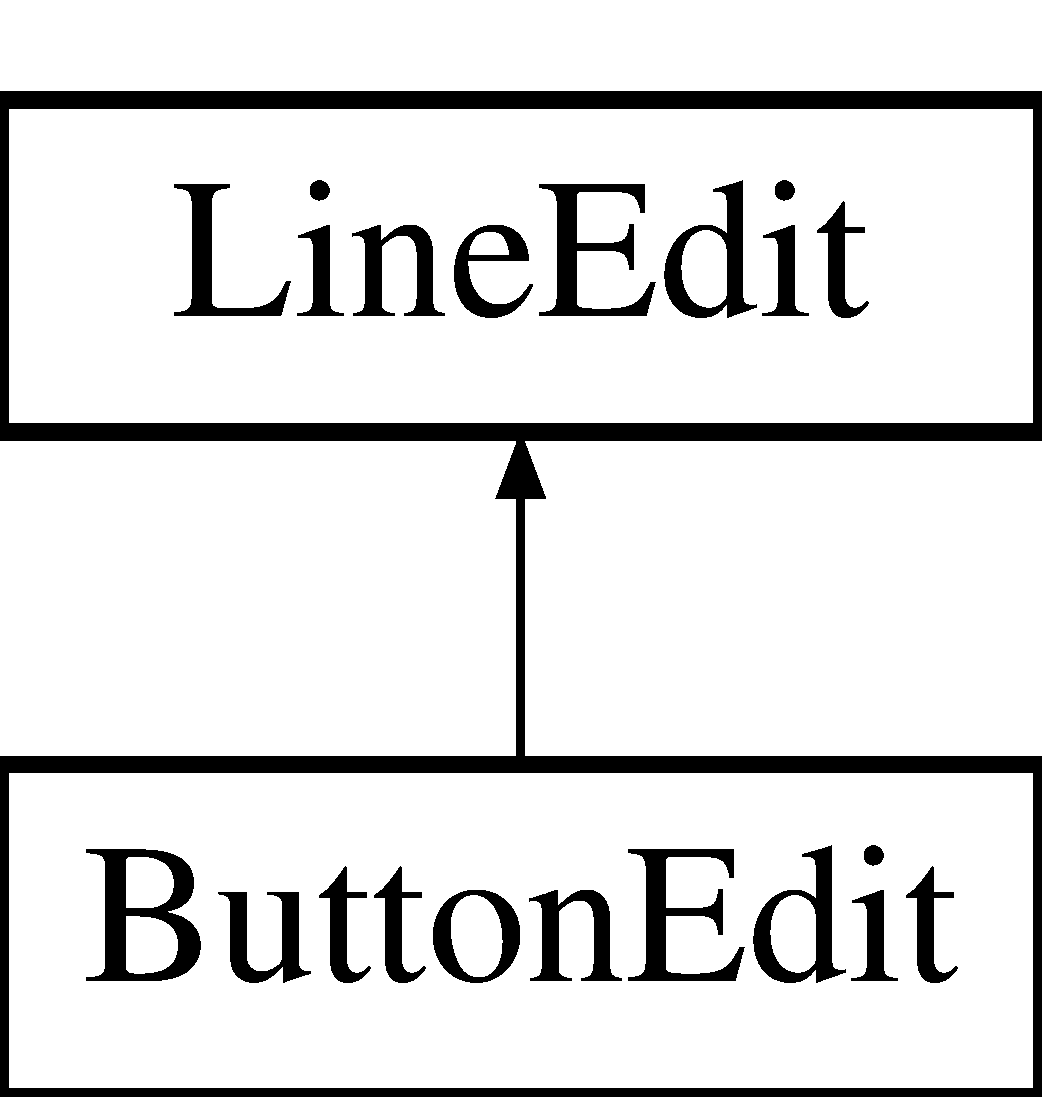
\includegraphics[height=2.000000cm]{classButtonEdit}
\end{center}
\end{figure}
\subsection*{Public Slots}
\begin{DoxyCompactItemize}
\item 
void \hyperlink{classButtonEdit_a5f122d262f539f9b4573f0038dee5b63}{buttonClicked} ()
\end{DoxyCompactItemize}
\subsection*{Public Member Functions}
\begin{DoxyCompactItemize}
\item 
\hyperlink{classButtonEdit_a9a6e3658bb796d5cd3ea99d1a19e8326}{ButtonEdit} (QString \hyperlink{classButtonEdit_a609d52554a0d2943f453d1cffc89c566}{iconFileName}=NULL, QWidget $\ast$parent=0)
\item 
void \hyperlink{classButtonEdit_a5d38b77fee50b8052338542e1ae568a9}{setButtonKey} (QString bk)
\item 
QString \hyperlink{classButtonEdit_a685a87378838136bd8b72443ddc888e8}{buttonKey} ()
\item 
QPushButton $\ast$ \hyperlink{classButtonEdit_a40c63eff1e9a16d817c017f629a4872f}{getButtonObj} ()
\end{DoxyCompactItemize}
\subsection*{Protected Member Functions}
\begin{DoxyCompactItemize}
\item 
void \hyperlink{classButtonEdit_a70d44e2f9fb64cad1656d4151c757de9}{resizeEvent} (QResizeEvent $\ast$)
\end{DoxyCompactItemize}
\subsection*{Private Attributes}
\begin{DoxyCompactItemize}
\item 
QPushButton $\ast$ \hyperlink{classButtonEdit_a8cf55e06c1f23cdd00622ea213f338d3}{button}
\item 
QString \hyperlink{classButtonEdit_a609d52554a0d2943f453d1cffc89c566}{iconFileName}
\item 
QString \hyperlink{classButtonEdit_a8eece0b4a3f4b5424ffe08985b9be8b6}{qs\_\-buttonKey}
\end{DoxyCompactItemize}


\subsection{Detailed Description}


Definition at line 224 of file vwidgets.h.



\subsection{Constructor \& Destructor Documentation}
\hypertarget{classButtonEdit_a9a6e3658bb796d5cd3ea99d1a19e8326}{
\index{ButtonEdit@{ButtonEdit}!ButtonEdit@{ButtonEdit}}
\index{ButtonEdit@{ButtonEdit}!ButtonEdit@{ButtonEdit}}
\subsubsection[{ButtonEdit}]{\setlength{\rightskip}{0pt plus 5cm}ButtonEdit::ButtonEdit (
\begin{DoxyParamCaption}
\item[{QString}]{iconFileName = {\ttfamily NULL}, }
\item[{QWidget $\ast$}]{parent = {\ttfamily 0}}
\end{DoxyParamCaption}
)}}
\label{classButtonEdit_a9a6e3658bb796d5cd3ea99d1a19e8326}


Definition at line 464 of file vwidgets.cpp.



\subsection{Member Function Documentation}
\hypertarget{classButtonEdit_a5f122d262f539f9b4573f0038dee5b63}{
\index{ButtonEdit@{ButtonEdit}!buttonClicked@{buttonClicked}}
\index{buttonClicked@{buttonClicked}!ButtonEdit@{ButtonEdit}}
\subsubsection[{buttonClicked}]{\setlength{\rightskip}{0pt plus 5cm}void ButtonEdit::buttonClicked (
\begin{DoxyParamCaption}
{}
\end{DoxyParamCaption}
)\hspace{0.3cm}{\ttfamily  \mbox{[}slot\mbox{]}}}}
\label{classButtonEdit_a5f122d262f539f9b4573f0038dee5b63}


Definition at line 523 of file vwidgets.cpp.

\hypertarget{classButtonEdit_a685a87378838136bd8b72443ddc888e8}{
\index{ButtonEdit@{ButtonEdit}!buttonKey@{buttonKey}}
\index{buttonKey@{buttonKey}!ButtonEdit@{ButtonEdit}}
\subsubsection[{buttonKey}]{\setlength{\rightskip}{0pt plus 5cm}QString ButtonEdit::buttonKey (
\begin{DoxyParamCaption}
{}
\end{DoxyParamCaption}
)\hspace{0.3cm}{\ttfamily  \mbox{[}inline\mbox{]}}}}
\label{classButtonEdit_a685a87378838136bd8b72443ddc888e8}


Definition at line 231 of file vwidgets.h.

\hypertarget{classButtonEdit_a40c63eff1e9a16d817c017f629a4872f}{
\index{ButtonEdit@{ButtonEdit}!getButtonObj@{getButtonObj}}
\index{getButtonObj@{getButtonObj}!ButtonEdit@{ButtonEdit}}
\subsubsection[{getButtonObj}]{\setlength{\rightskip}{0pt plus 5cm}QPushButton $\ast$ ButtonEdit::getButtonObj (
\begin{DoxyParamCaption}
{}
\end{DoxyParamCaption}
)}}
\label{classButtonEdit_a40c63eff1e9a16d817c017f629a4872f}


Definition at line 504 of file vwidgets.cpp.

\hypertarget{classButtonEdit_a70d44e2f9fb64cad1656d4151c757de9}{
\index{ButtonEdit@{ButtonEdit}!resizeEvent@{resizeEvent}}
\index{resizeEvent@{resizeEvent}!ButtonEdit@{ButtonEdit}}
\subsubsection[{resizeEvent}]{\setlength{\rightskip}{0pt plus 5cm}void ButtonEdit::resizeEvent (
\begin{DoxyParamCaption}
\item[{QResizeEvent $\ast$}]{}
\end{DoxyParamCaption}
)\hspace{0.3cm}{\ttfamily  \mbox{[}protected\mbox{]}}}}
\label{classButtonEdit_a70d44e2f9fb64cad1656d4151c757de9}


Definition at line 510 of file vwidgets.cpp.

\hypertarget{classButtonEdit_a5d38b77fee50b8052338542e1ae568a9}{
\index{ButtonEdit@{ButtonEdit}!setButtonKey@{setButtonKey}}
\index{setButtonKey@{setButtonKey}!ButtonEdit@{ButtonEdit}}
\subsubsection[{setButtonKey}]{\setlength{\rightskip}{0pt plus 5cm}void ButtonEdit::setButtonKey (
\begin{DoxyParamCaption}
\item[{QString}]{bk}
\end{DoxyParamCaption}
)}}
\label{classButtonEdit_a5d38b77fee50b8052338542e1ae568a9}


Definition at line 491 of file vwidgets.cpp.



\subsection{Member Data Documentation}
\hypertarget{classButtonEdit_a8cf55e06c1f23cdd00622ea213f338d3}{
\index{ButtonEdit@{ButtonEdit}!button@{button}}
\index{button@{button}!ButtonEdit@{ButtonEdit}}
\subsubsection[{button}]{\setlength{\rightskip}{0pt plus 5cm}QPushButton$\ast$ {\bf ButtonEdit::button}\hspace{0.3cm}{\ttfamily  \mbox{[}private\mbox{]}}}}
\label{classButtonEdit_a8cf55e06c1f23cdd00622ea213f338d3}


Definition at line 235 of file vwidgets.h.

\hypertarget{classButtonEdit_a609d52554a0d2943f453d1cffc89c566}{
\index{ButtonEdit@{ButtonEdit}!iconFileName@{iconFileName}}
\index{iconFileName@{iconFileName}!ButtonEdit@{ButtonEdit}}
\subsubsection[{iconFileName}]{\setlength{\rightskip}{0pt plus 5cm}QString {\bf ButtonEdit::iconFileName}\hspace{0.3cm}{\ttfamily  \mbox{[}private\mbox{]}}}}
\label{classButtonEdit_a609d52554a0d2943f453d1cffc89c566}


Definition at line 236 of file vwidgets.h.

\hypertarget{classButtonEdit_a8eece0b4a3f4b5424ffe08985b9be8b6}{
\index{ButtonEdit@{ButtonEdit}!qs\_\-buttonKey@{qs\_\-buttonKey}}
\index{qs\_\-buttonKey@{qs\_\-buttonKey}!ButtonEdit@{ButtonEdit}}
\subsubsection[{qs\_\-buttonKey}]{\setlength{\rightskip}{0pt plus 5cm}QString {\bf ButtonEdit::qs\_\-buttonKey}\hspace{0.3cm}{\ttfamily  \mbox{[}private\mbox{]}}}}
\label{classButtonEdit_a8eece0b4a3f4b5424ffe08985b9be8b6}


Definition at line 237 of file vwidgets.h.



The documentation for this class was generated from the following files:\begin{DoxyCompactItemize}
\item 
/e/ms/QT/models/\hyperlink{vwidgets_8h}{vwidgets.h}\item 
/e/ms/QT/models/\hyperlink{vwidgets_8cpp}{vwidgets.cpp}\end{DoxyCompactItemize}

\hypertarget{classCalendar}{
\section{Calendar Class Reference}
\label{classCalendar}\index{Calendar@{Calendar}}
}


{\ttfamily \#include $<$vwidgets.h$>$}

\subsection*{Public Slots}
\begin{DoxyCompactItemize}
\item 
void \hyperlink{classCalendar_acd4839649c97f51c23c64820e64132c0}{setDay} ()
\end{DoxyCompactItemize}
\subsection*{Public Member Functions}
\begin{DoxyCompactItemize}
\item 
\hyperlink{classCalendar_a08e64d2af594c9cd1f457940ccd24b87}{Calendar} (QWidget $\ast$parent=0, QLineEdit $\ast$sender=0)
\end{DoxyCompactItemize}
\subsection*{Public Attributes}
\begin{DoxyCompactItemize}
\item 
QDate \hyperlink{classCalendar_a8833e2da3604d141186517e4d33b9723}{day}
\item 
QLineEdit $\ast$ \hyperlink{classCalendar_a12e11b519eea5eaa74d6dc5f9e1c5520}{dateEdit}
\end{DoxyCompactItemize}


\subsection{Detailed Description}


Definition at line 545 of file vwidgets.h.



\subsection{Constructor \& Destructor Documentation}
\hypertarget{classCalendar_a08e64d2af594c9cd1f457940ccd24b87}{
\index{Calendar@{Calendar}!Calendar@{Calendar}}
\index{Calendar@{Calendar}!Calendar@{Calendar}}
\subsubsection[{Calendar}]{\setlength{\rightskip}{0pt plus 5cm}Calendar::Calendar (
\begin{DoxyParamCaption}
\item[{QWidget $\ast$}]{parent = {\ttfamily 0}, }
\item[{QLineEdit $\ast$}]{sender = {\ttfamily 0}}
\end{DoxyParamCaption}
)}}
\label{classCalendar_a08e64d2af594c9cd1f457940ccd24b87}


Definition at line 2396 of file vwidgets.cpp.



\subsection{Member Function Documentation}
\hypertarget{classCalendar_acd4839649c97f51c23c64820e64132c0}{
\index{Calendar@{Calendar}!setDay@{setDay}}
\index{setDay@{setDay}!Calendar@{Calendar}}
\subsubsection[{setDay}]{\setlength{\rightskip}{0pt plus 5cm}void Calendar::setDay (
\begin{DoxyParamCaption}
{}
\end{DoxyParamCaption}
)\hspace{0.3cm}{\ttfamily  \mbox{[}slot\mbox{]}}}}
\label{classCalendar_acd4839649c97f51c23c64820e64132c0}


Definition at line 2406 of file vwidgets.cpp.



\subsection{Member Data Documentation}
\hypertarget{classCalendar_a12e11b519eea5eaa74d6dc5f9e1c5520}{
\index{Calendar@{Calendar}!dateEdit@{dateEdit}}
\index{dateEdit@{dateEdit}!Calendar@{Calendar}}
\subsubsection[{dateEdit}]{\setlength{\rightskip}{0pt plus 5cm}QLineEdit$\ast$ {\bf Calendar::dateEdit}}}
\label{classCalendar_a12e11b519eea5eaa74d6dc5f9e1c5520}


Definition at line 552 of file vwidgets.h.

\hypertarget{classCalendar_a8833e2da3604d141186517e4d33b9723}{
\index{Calendar@{Calendar}!day@{day}}
\index{day@{day}!Calendar@{Calendar}}
\subsubsection[{day}]{\setlength{\rightskip}{0pt plus 5cm}QDate {\bf Calendar::day}}}
\label{classCalendar_a8833e2da3604d141186517e4d33b9723}


Definition at line 551 of file vwidgets.h.



The documentation for this class was generated from the following files:\begin{DoxyCompactItemize}
\item 
/e/ms/QT/models/\hyperlink{vwidgets_8h}{vwidgets.h}\item 
/e/ms/QT/models/\hyperlink{vwidgets_8cpp}{vwidgets.cpp}\end{DoxyCompactItemize}

\hypertarget{classCheckBox}{
\section{CheckBox Class Reference}
\label{classCheckBox}\index{CheckBox@{CheckBox}}
}


{\ttfamily \#include $<$vwidgets.h$>$}

\subsection*{Signals}
\begin{DoxyCompactItemize}
\item 
void \hyperlink{classCheckBox_ab7701c08638ff1fcdbda78bd9da08467}{fieldEvent} (\hyperlink{structFgl_1_1Event}{Fgl::Event})
\end{DoxyCompactItemize}
\subsection*{Public Member Functions}
\begin{DoxyCompactItemize}
\item 
\hyperlink{classCheckBox_a1142cc2820e6e1bd93a1c4a971774c34}{CheckBox} (QWidget $\ast$parent=NULL)
\item 
\hyperlink{classCheckBox_ab7c41072f6ba5f744f942b1962a14869}{CheckBox} (QString, QWidget $\ast$parent=NULL)
\item 
void \hyperlink{classCheckBox_aeda5bfde9248d30788390239d241ee69}{setValueChecked} (QString val)
\item 
QString \hyperlink{classCheckBox_a33e6aa1e2b208c4ad636cfe2652afd56}{valueChecked} ()
\item 
void \hyperlink{classCheckBox_a2ee08e32b608ef954f9cdaa7366a8285}{setValueUnchecked} (QString val)
\item 
QString \hyperlink{classCheckBox_a744b38f582ab963ba3a671862e8df5d6}{valueUnchecked} ()
\item 
void \hyperlink{classCheckBox_a1248f1fb389c4b3960ccf32e37b22b57}{setDefaultValue} (QString def)
\item 
QString \hyperlink{classCheckBox_afa6cf2c41430d4ee7b00b0902c12c7e8}{defaultValue} ()
\end{DoxyCompactItemize}
\subsection*{Private Attributes}
\begin{DoxyCompactItemize}
\item 
QString \hyperlink{classCheckBox_a44ec1015259303e99d56c04fe5841e39}{qs\_\-valueChecked}
\item 
QString \hyperlink{classCheckBox_aad5473314931f69256aabde7f44c473a}{qs\_\-valueUnchecked}
\item 
QString \hyperlink{classCheckBox_ac21bfd62bb71d0dd23f72e6ef70293d6}{qs\_\-default}
\end{DoxyCompactItemize}


\subsection{Detailed Description}


Definition at line 268 of file vwidgets.h.



\subsection{Constructor \& Destructor Documentation}
\hypertarget{classCheckBox_a1142cc2820e6e1bd93a1c4a971774c34}{
\index{CheckBox@{CheckBox}!CheckBox@{CheckBox}}
\index{CheckBox@{CheckBox}!CheckBox@{CheckBox}}
\subsubsection[{CheckBox}]{\setlength{\rightskip}{0pt plus 5cm}CheckBox::CheckBox (
\begin{DoxyParamCaption}
\item[{QWidget $\ast$}]{parent = {\ttfamily NULL}}
\end{DoxyParamCaption}
)}}
\label{classCheckBox_a1142cc2820e6e1bd93a1c4a971774c34}


Definition at line 2438 of file vwidgets.cpp.

\hypertarget{classCheckBox_ab7c41072f6ba5f744f942b1962a14869}{
\index{CheckBox@{CheckBox}!CheckBox@{CheckBox}}
\index{CheckBox@{CheckBox}!CheckBox@{CheckBox}}
\subsubsection[{CheckBox}]{\setlength{\rightskip}{0pt plus 5cm}CheckBox::CheckBox (
\begin{DoxyParamCaption}
\item[{QString}]{text, }
\item[{QWidget $\ast$}]{parent = {\ttfamily NULL}}
\end{DoxyParamCaption}
)}}
\label{classCheckBox_ab7c41072f6ba5f744f942b1962a14869}


Definition at line 2448 of file vwidgets.cpp.



\subsection{Member Function Documentation}
\hypertarget{classCheckBox_afa6cf2c41430d4ee7b00b0902c12c7e8}{
\index{CheckBox@{CheckBox}!defaultValue@{defaultValue}}
\index{defaultValue@{defaultValue}!CheckBox@{CheckBox}}
\subsubsection[{defaultValue}]{\setlength{\rightskip}{0pt plus 5cm}QString CheckBox::defaultValue (
\begin{DoxyParamCaption}
{}
\end{DoxyParamCaption}
)\hspace{0.3cm}{\ttfamily  \mbox{[}inline\mbox{]}}}}
\label{classCheckBox_afa6cf2c41430d4ee7b00b0902c12c7e8}


Definition at line 281 of file vwidgets.h.

\hypertarget{classCheckBox_ab7701c08638ff1fcdbda78bd9da08467}{
\index{CheckBox@{CheckBox}!fieldEvent@{fieldEvent}}
\index{fieldEvent@{fieldEvent}!CheckBox@{CheckBox}}
\subsubsection[{fieldEvent}]{\setlength{\rightskip}{0pt plus 5cm}void CheckBox::fieldEvent (
\begin{DoxyParamCaption}
\item[{{\bf Fgl::Event}}]{}
\end{DoxyParamCaption}
)\hspace{0.3cm}{\ttfamily  \mbox{[}signal\mbox{]}}}}
\label{classCheckBox_ab7701c08638ff1fcdbda78bd9da08467}
\hypertarget{classCheckBox_a1248f1fb389c4b3960ccf32e37b22b57}{
\index{CheckBox@{CheckBox}!setDefaultValue@{setDefaultValue}}
\index{setDefaultValue@{setDefaultValue}!CheckBox@{CheckBox}}
\subsubsection[{setDefaultValue}]{\setlength{\rightskip}{0pt plus 5cm}void CheckBox::setDefaultValue (
\begin{DoxyParamCaption}
\item[{QString}]{def}
\end{DoxyParamCaption}
)\hspace{0.3cm}{\ttfamily  \mbox{[}inline\mbox{]}}}}
\label{classCheckBox_a1248f1fb389c4b3960ccf32e37b22b57}


Definition at line 280 of file vwidgets.h.

\hypertarget{classCheckBox_aeda5bfde9248d30788390239d241ee69}{
\index{CheckBox@{CheckBox}!setValueChecked@{setValueChecked}}
\index{setValueChecked@{setValueChecked}!CheckBox@{CheckBox}}
\subsubsection[{setValueChecked}]{\setlength{\rightskip}{0pt plus 5cm}void CheckBox::setValueChecked (
\begin{DoxyParamCaption}
\item[{QString}]{val}
\end{DoxyParamCaption}
)\hspace{0.3cm}{\ttfamily  \mbox{[}inline\mbox{]}}}}
\label{classCheckBox_aeda5bfde9248d30788390239d241ee69}


Definition at line 276 of file vwidgets.h.

\hypertarget{classCheckBox_a2ee08e32b608ef954f9cdaa7366a8285}{
\index{CheckBox@{CheckBox}!setValueUnchecked@{setValueUnchecked}}
\index{setValueUnchecked@{setValueUnchecked}!CheckBox@{CheckBox}}
\subsubsection[{setValueUnchecked}]{\setlength{\rightskip}{0pt plus 5cm}void CheckBox::setValueUnchecked (
\begin{DoxyParamCaption}
\item[{QString}]{val}
\end{DoxyParamCaption}
)\hspace{0.3cm}{\ttfamily  \mbox{[}inline\mbox{]}}}}
\label{classCheckBox_a2ee08e32b608ef954f9cdaa7366a8285}


Definition at line 278 of file vwidgets.h.

\hypertarget{classCheckBox_a33e6aa1e2b208c4ad636cfe2652afd56}{
\index{CheckBox@{CheckBox}!valueChecked@{valueChecked}}
\index{valueChecked@{valueChecked}!CheckBox@{CheckBox}}
\subsubsection[{valueChecked}]{\setlength{\rightskip}{0pt plus 5cm}QString CheckBox::valueChecked (
\begin{DoxyParamCaption}
{}
\end{DoxyParamCaption}
)\hspace{0.3cm}{\ttfamily  \mbox{[}inline\mbox{]}}}}
\label{classCheckBox_a33e6aa1e2b208c4ad636cfe2652afd56}


Definition at line 277 of file vwidgets.h.

\hypertarget{classCheckBox_a744b38f582ab963ba3a671862e8df5d6}{
\index{CheckBox@{CheckBox}!valueUnchecked@{valueUnchecked}}
\index{valueUnchecked@{valueUnchecked}!CheckBox@{CheckBox}}
\subsubsection[{valueUnchecked}]{\setlength{\rightskip}{0pt plus 5cm}QString CheckBox::valueUnchecked (
\begin{DoxyParamCaption}
{}
\end{DoxyParamCaption}
)\hspace{0.3cm}{\ttfamily  \mbox{[}inline\mbox{]}}}}
\label{classCheckBox_a744b38f582ab963ba3a671862e8df5d6}


Definition at line 279 of file vwidgets.h.



\subsection{Member Data Documentation}
\hypertarget{classCheckBox_ac21bfd62bb71d0dd23f72e6ef70293d6}{
\index{CheckBox@{CheckBox}!qs\_\-default@{qs\_\-default}}
\index{qs\_\-default@{qs\_\-default}!CheckBox@{CheckBox}}
\subsubsection[{qs\_\-default}]{\setlength{\rightskip}{0pt plus 5cm}QString {\bf CheckBox::qs\_\-default}\hspace{0.3cm}{\ttfamily  \mbox{[}private\mbox{]}}}}
\label{classCheckBox_ac21bfd62bb71d0dd23f72e6ef70293d6}


Definition at line 286 of file vwidgets.h.

\hypertarget{classCheckBox_a44ec1015259303e99d56c04fe5841e39}{
\index{CheckBox@{CheckBox}!qs\_\-valueChecked@{qs\_\-valueChecked}}
\index{qs\_\-valueChecked@{qs\_\-valueChecked}!CheckBox@{CheckBox}}
\subsubsection[{qs\_\-valueChecked}]{\setlength{\rightskip}{0pt plus 5cm}QString {\bf CheckBox::qs\_\-valueChecked}\hspace{0.3cm}{\ttfamily  \mbox{[}private\mbox{]}}}}
\label{classCheckBox_a44ec1015259303e99d56c04fe5841e39}


Definition at line 281 of file vwidgets.h.

\hypertarget{classCheckBox_aad5473314931f69256aabde7f44c473a}{
\index{CheckBox@{CheckBox}!qs\_\-valueUnchecked@{qs\_\-valueUnchecked}}
\index{qs\_\-valueUnchecked@{qs\_\-valueUnchecked}!CheckBox@{CheckBox}}
\subsubsection[{qs\_\-valueUnchecked}]{\setlength{\rightskip}{0pt plus 5cm}QString {\bf CheckBox::qs\_\-valueUnchecked}\hspace{0.3cm}{\ttfamily  \mbox{[}private\mbox{]}}}}
\label{classCheckBox_aad5473314931f69256aabde7f44c473a}


Definition at line 285 of file vwidgets.h.



The documentation for this class was generated from the following files:\begin{DoxyCompactItemize}
\item 
/e/ms/QT/models/\hyperlink{vwidgets_8h}{vwidgets.h}\item 
/e/ms/QT/models/\hyperlink{vwidgets_8cpp}{vwidgets.cpp}\end{DoxyCompactItemize}

\hypertarget{classComboBox}{
\section{ComboBox Class Reference}
\label{classComboBox}\index{ComboBox@{ComboBox}}
}


{\ttfamily \#include $<$vwidgets.h$>$}

\subsection*{Signals}
\begin{DoxyCompactItemize}
\item 
void \hyperlink{classComboBox_a42cbdd334cab08f8cd64f4fc2a491eab}{fieldEvent} (\hyperlink{structFgl_1_1Event}{Fgl::Event})
\end{DoxyCompactItemize}
\subsection*{Public Member Functions}
\begin{DoxyCompactItemize}
\item 
\hyperlink{classComboBox_a32bb4cff0a07749af81ed8a7611a87ea}{ComboBox} (QWidget $\ast$parent=0)
\item 
void \hyperlink{classComboBox_a11c773791207b37ea0a4d68bc99d1514}{setDefaultValue} (QString def)
\item 
QString \hyperlink{classComboBox_ab48383251ec25b0144e22d2cbaf4d796}{defaultValue} ()
\end{DoxyCompactItemize}
\subsection*{Public Attributes}
\begin{DoxyCompactItemize}
\item 
QString \hyperlink{classComboBox_aba2d3d19c110bea05059e80a6125f976}{colName}
\item 
QString \hyperlink{classComboBox_a9c2352629cde1787cc7a10ea998168d1}{sqlTabName}
\end{DoxyCompactItemize}
\subsection*{Private Attributes}
\begin{DoxyCompactItemize}
\item 
QString \hyperlink{classComboBox_a945d7dffb6e4343ecbdc550f287a3c9a}{qs\_\-default}
\end{DoxyCompactItemize}


\subsection{Detailed Description}


Definition at line 250 of file vwidgets.h.



\subsection{Constructor \& Destructor Documentation}
\hypertarget{classComboBox_a32bb4cff0a07749af81ed8a7611a87ea}{
\index{ComboBox@{ComboBox}!ComboBox@{ComboBox}}
\index{ComboBox@{ComboBox}!ComboBox@{ComboBox}}
\subsubsection[{ComboBox}]{\setlength{\rightskip}{0pt plus 5cm}ComboBox::ComboBox (
\begin{DoxyParamCaption}
\item[{QWidget $\ast$}]{parent = {\ttfamily 0}}
\end{DoxyParamCaption}
)}}
\label{classComboBox_a32bb4cff0a07749af81ed8a7611a87ea}


Definition at line 2424 of file vwidgets.cpp.



\subsection{Member Function Documentation}
\hypertarget{classComboBox_ab48383251ec25b0144e22d2cbaf4d796}{
\index{ComboBox@{ComboBox}!defaultValue@{defaultValue}}
\index{defaultValue@{defaultValue}!ComboBox@{ComboBox}}
\subsubsection[{defaultValue}]{\setlength{\rightskip}{0pt plus 5cm}QString ComboBox::defaultValue (
\begin{DoxyParamCaption}
{}
\end{DoxyParamCaption}
)\hspace{0.3cm}{\ttfamily  \mbox{[}inline\mbox{]}}}}
\label{classComboBox_ab48383251ec25b0144e22d2cbaf4d796}


Definition at line 257 of file vwidgets.h.

\hypertarget{classComboBox_a42cbdd334cab08f8cd64f4fc2a491eab}{
\index{ComboBox@{ComboBox}!fieldEvent@{fieldEvent}}
\index{fieldEvent@{fieldEvent}!ComboBox@{ComboBox}}
\subsubsection[{fieldEvent}]{\setlength{\rightskip}{0pt plus 5cm}void ComboBox::fieldEvent (
\begin{DoxyParamCaption}
\item[{{\bf Fgl::Event}}]{}
\end{DoxyParamCaption}
)\hspace{0.3cm}{\ttfamily  \mbox{[}signal\mbox{]}}}}
\label{classComboBox_a42cbdd334cab08f8cd64f4fc2a491eab}
\hypertarget{classComboBox_a11c773791207b37ea0a4d68bc99d1514}{
\index{ComboBox@{ComboBox}!setDefaultValue@{setDefaultValue}}
\index{setDefaultValue@{setDefaultValue}!ComboBox@{ComboBox}}
\subsubsection[{setDefaultValue}]{\setlength{\rightskip}{0pt plus 5cm}void ComboBox::setDefaultValue (
\begin{DoxyParamCaption}
\item[{QString}]{def}
\end{DoxyParamCaption}
)\hspace{0.3cm}{\ttfamily  \mbox{[}inline\mbox{]}}}}
\label{classComboBox_a11c773791207b37ea0a4d68bc99d1514}


Definition at line 256 of file vwidgets.h.



\subsection{Member Data Documentation}
\hypertarget{classComboBox_aba2d3d19c110bea05059e80a6125f976}{
\index{ComboBox@{ComboBox}!colName@{colName}}
\index{colName@{colName}!ComboBox@{ComboBox}}
\subsubsection[{colName}]{\setlength{\rightskip}{0pt plus 5cm}QString {\bf ComboBox::colName}}}
\label{classComboBox_aba2d3d19c110bea05059e80a6125f976}


Definition at line 257 of file vwidgets.h.

\hypertarget{classComboBox_a945d7dffb6e4343ecbdc550f287a3c9a}{
\index{ComboBox@{ComboBox}!qs\_\-default@{qs\_\-default}}
\index{qs\_\-default@{qs\_\-default}!ComboBox@{ComboBox}}
\subsubsection[{qs\_\-default}]{\setlength{\rightskip}{0pt plus 5cm}QString {\bf ComboBox::qs\_\-default}\hspace{0.3cm}{\ttfamily  \mbox{[}private\mbox{]}}}}
\label{classComboBox_a945d7dffb6e4343ecbdc550f287a3c9a}


Definition at line 262 of file vwidgets.h.

\hypertarget{classComboBox_a9c2352629cde1787cc7a10ea998168d1}{
\index{ComboBox@{ComboBox}!sqlTabName@{sqlTabName}}
\index{sqlTabName@{sqlTabName}!ComboBox@{ComboBox}}
\subsubsection[{sqlTabName}]{\setlength{\rightskip}{0pt plus 5cm}QString {\bf ComboBox::sqlTabName}}}
\label{classComboBox_a9c2352629cde1787cc7a10ea998168d1}


Definition at line 259 of file vwidgets.h.



The documentation for this class was generated from the following files:\begin{DoxyCompactItemize}
\item 
/e/ms/QT/models/\hyperlink{vwidgets_8h}{vwidgets.h}\item 
/e/ms/QT/models/\hyperlink{vwidgets_8cpp}{vwidgets.cpp}\end{DoxyCompactItemize}

\hypertarget{classDateEdit}{
\section{DateEdit Class Reference}
\label{classDateEdit}\index{DateEdit@{DateEdit}}
}


{\ttfamily \#include $<$vwidgets.h$>$}

Inheritance diagram for DateEdit:\begin{figure}[H]
\begin{center}
\leavevmode
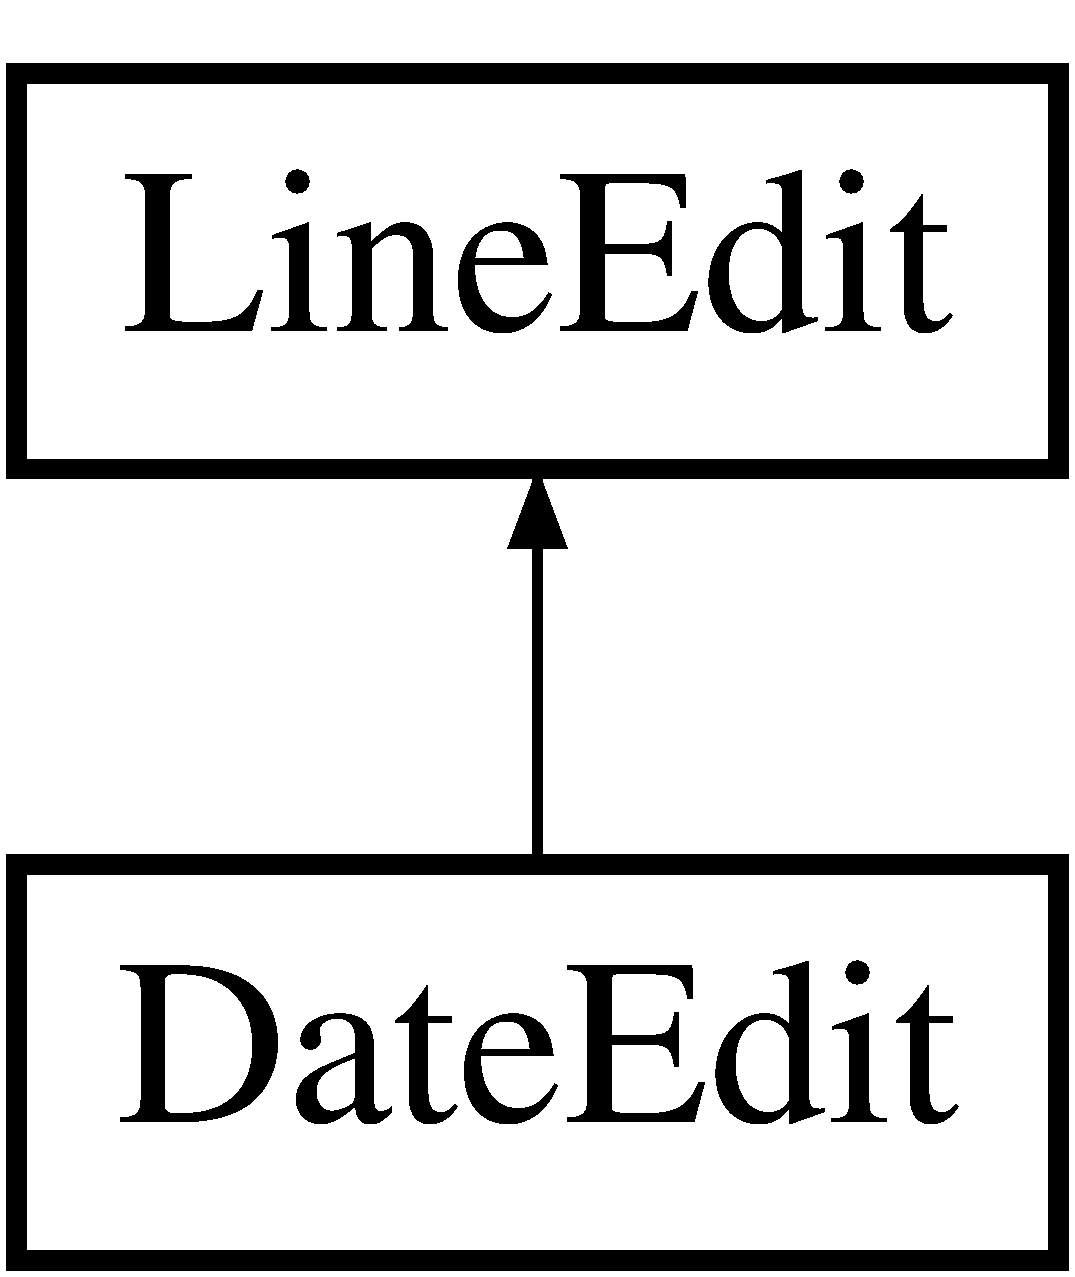
\includegraphics[height=2.000000cm]{classDateEdit}
\end{center}
\end{figure}
\subsection*{Public Slots}
\begin{DoxyCompactItemize}
\item 
void \hyperlink{classDateEdit_a4f16955de169de197867b3298592ce3e}{buttonClicked} ()
\end{DoxyCompactItemize}
\subsection*{Public Member Functions}
\begin{DoxyCompactItemize}
\item 
\hyperlink{classDateEdit_a2419b5b3044083ab297107966ba4b310}{DateEdit} (QWidget $\ast$parent=0)
\end{DoxyCompactItemize}
\subsection*{Protected Member Functions}
\begin{DoxyCompactItemize}
\item 
void \hyperlink{classDateEdit_a84296994dc057b587ea9542604a3e050}{resizeEvent} (QResizeEvent $\ast$)
\end{DoxyCompactItemize}
\subsection*{Private Attributes}
\begin{DoxyCompactItemize}
\item 
QPushButton $\ast$ \hyperlink{classDateEdit_a54dc3b413c28dac9aa044d185b17bccf}{button}
\item 
QString \hyperlink{classDateEdit_a79214d87b36dc55ec6f783fa287d238d}{iconFileName}
\end{DoxyCompactItemize}


\subsection{Detailed Description}


Definition at line 292 of file vwidgets.h.



\subsection{Constructor \& Destructor Documentation}
\hypertarget{classDateEdit_a2419b5b3044083ab297107966ba4b310}{
\index{DateEdit@{DateEdit}!DateEdit@{DateEdit}}
\index{DateEdit@{DateEdit}!DateEdit@{DateEdit}}
\subsubsection[{DateEdit}]{\setlength{\rightskip}{0pt plus 5cm}DateEdit::DateEdit (
\begin{DoxyParamCaption}
\item[{QWidget $\ast$}]{parent = {\ttfamily 0}}
\end{DoxyParamCaption}
)}}
\label{classDateEdit_a2419b5b3044083ab297107966ba4b310}


Definition at line 542 of file vwidgets.cpp.



\subsection{Member Function Documentation}
\hypertarget{classDateEdit_a4f16955de169de197867b3298592ce3e}{
\index{DateEdit@{DateEdit}!buttonClicked@{buttonClicked}}
\index{buttonClicked@{buttonClicked}!DateEdit@{DateEdit}}
\subsubsection[{buttonClicked}]{\setlength{\rightskip}{0pt plus 5cm}void DateEdit::buttonClicked (
\begin{DoxyParamCaption}
{}
\end{DoxyParamCaption}
)\hspace{0.3cm}{\ttfamily  \mbox{[}slot\mbox{]}}}}
\label{classDateEdit_a4f16955de169de197867b3298592ce3e}


Definition at line 573 of file vwidgets.cpp.

\hypertarget{classDateEdit_a84296994dc057b587ea9542604a3e050}{
\index{DateEdit@{DateEdit}!resizeEvent@{resizeEvent}}
\index{resizeEvent@{resizeEvent}!DateEdit@{DateEdit}}
\subsubsection[{resizeEvent}]{\setlength{\rightskip}{0pt plus 5cm}void DateEdit::resizeEvent (
\begin{DoxyParamCaption}
\item[{QResizeEvent $\ast$}]{}
\end{DoxyParamCaption}
)\hspace{0.3cm}{\ttfamily  \mbox{[}protected\mbox{]}}}}
\label{classDateEdit_a84296994dc057b587ea9542604a3e050}


Definition at line 565 of file vwidgets.cpp.



\subsection{Member Data Documentation}
\hypertarget{classDateEdit_a54dc3b413c28dac9aa044d185b17bccf}{
\index{DateEdit@{DateEdit}!button@{button}}
\index{button@{button}!DateEdit@{DateEdit}}
\subsubsection[{button}]{\setlength{\rightskip}{0pt plus 5cm}QPushButton$\ast$ {\bf DateEdit::button}\hspace{0.3cm}{\ttfamily  \mbox{[}private\mbox{]}}}}
\label{classDateEdit_a54dc3b413c28dac9aa044d185b17bccf}


Definition at line 303 of file vwidgets.h.

\hypertarget{classDateEdit_a79214d87b36dc55ec6f783fa287d238d}{
\index{DateEdit@{DateEdit}!iconFileName@{iconFileName}}
\index{iconFileName@{iconFileName}!DateEdit@{DateEdit}}
\subsubsection[{iconFileName}]{\setlength{\rightskip}{0pt plus 5cm}QString {\bf DateEdit::iconFileName}\hspace{0.3cm}{\ttfamily  \mbox{[}private\mbox{]}}}}
\label{classDateEdit_a79214d87b36dc55ec6f783fa287d238d}


Definition at line 304 of file vwidgets.h.



The documentation for this class was generated from the following files:\begin{DoxyCompactItemize}
\item 
/e/ms/QT/models/\hyperlink{vwidgets_8h}{vwidgets.h}\item 
/e/ms/QT/models/\hyperlink{vwidgets_8cpp}{vwidgets.cpp}\end{DoxyCompactItemize}

\hypertarget{classDialog}{
\section{Dialog Class Reference}
\label{classDialog}\index{Dialog@{Dialog}}
}


{\ttfamily \#include $<$dialog.h$>$}

\subsection*{Public Slots}
\begin{DoxyCompactItemize}
\item 
void \hyperlink{classDialog_a6fa11449e967bd9aba0e6afe89a5ad1a}{buttonClicked} (int)
\end{DoxyCompactItemize}
\subsection*{Signals}
\begin{DoxyCompactItemize}
\item 
void \hyperlink{classDialog_a0e8bd522a50e34e2edee2c6f64cf0399}{dialogButtonPressed} (QString)
\end{DoxyCompactItemize}
\subsection*{Public Member Functions}
\begin{DoxyCompactItemize}
\item 
\hyperlink{classDialog_a762d6d1bbcb935f48ce8a5debf7ce56e}{Dialog} (QString, QString, QString, QString, QWidget $\ast$parent=0, Qt::WindowFlags f=0)
\item 
\hyperlink{classDialog_a34b8d24a06d2d7cc90b2899b9acddd07}{Dialog} (QWidget $\ast$parent=0, Qt::WindowFlags f=0)
\item 
void \hyperlink{classDialog_afdfc6edcd72cc3f41e7ca5f4fc2499e5}{createButton} (int id=0, QString text=\char`\"{}\char`\"{}, QString desc=\char`\"{}\char`\"{}, QString icon=\char`\"{}\char`\"{})
\item 
void \hyperlink{classDialog_aebe85fc2c90f9418802687d1e0658548}{createAction} (int id=0, QString text=\char`\"{}\char`\"{})
\item 
void \hyperlink{classDialog_aa5d0ff2444e0d905bba16b0d82687f7b}{hideButton} (QString)
\item 
void \hyperlink{classDialog_aebbcfbdeabec1995374e3c37b248254f}{showButton} (QString)
\item 
QList$<$ QAction $\ast$ $>$ \hyperlink{classDialog_a583d6db9f52b55c8dae6bce5c85bfb14}{actions} ()
\item 
QAction $\ast$ \hyperlink{classDialog_a398e67a3c6eee5bbb9ed97d092211c62}{getAction} (QString)
\end{DoxyCompactItemize}
\subsection*{Protected Member Functions}
\begin{DoxyCompactItemize}
\item 
void \hyperlink{classDialog_aa687205f957253ec53f4ce47b49d302b}{keyPressEvent} (QKeyEvent $\ast$event)
\end{DoxyCompactItemize}
\subsection*{Private Attributes}
\begin{DoxyCompactItemize}
\item 
QLayout $\ast$ \hyperlink{classDialog_ad114214ed45b9210050334b5bde25250}{layout}
\item 
QLayout $\ast$ \hyperlink{classDialog_ad36793f71df8daf4e41ec4399d363985}{buttonLayout}
\item 
QButtonGroup $\ast$ \hyperlink{classDialog_a97288373583dd9aef3759869db27d5ff}{buttonGroup}
\end{DoxyCompactItemize}


\subsection{Detailed Description}


Definition at line 26 of file dialog.h.



\subsection{Constructor \& Destructor Documentation}
\hypertarget{classDialog_a762d6d1bbcb935f48ce8a5debf7ce56e}{
\index{Dialog@{Dialog}!Dialog@{Dialog}}
\index{Dialog@{Dialog}!Dialog@{Dialog}}
\subsubsection[{Dialog}]{\setlength{\rightskip}{0pt plus 5cm}Dialog::Dialog (
\begin{DoxyParamCaption}
\item[{QString}]{title, }
\item[{QString}]{comment, }
\item[{QString}]{style, }
\item[{QString}]{image, }
\item[{QWidget $\ast$}]{parent = {\ttfamily 0}, }
\item[{Qt::WindowFlags}]{f = {\ttfamily 0}}
\end{DoxyParamCaption}
)}}
\label{classDialog_a762d6d1bbcb935f48ce8a5debf7ce56e}


Definition at line 42 of file dialog.cpp.

\hypertarget{classDialog_a34b8d24a06d2d7cc90b2899b9acddd07}{
\index{Dialog@{Dialog}!Dialog@{Dialog}}
\index{Dialog@{Dialog}!Dialog@{Dialog}}
\subsubsection[{Dialog}]{\setlength{\rightskip}{0pt plus 5cm}Dialog::Dialog (
\begin{DoxyParamCaption}
\item[{QWidget $\ast$}]{parent = {\ttfamily 0}, }
\item[{Qt::WindowFlags}]{f = {\ttfamily 0}}
\end{DoxyParamCaption}
)}}
\label{classDialog_a34b8d24a06d2d7cc90b2899b9acddd07}


Definition at line 31 of file dialog.cpp.



\subsection{Member Function Documentation}
\hypertarget{classDialog_a583d6db9f52b55c8dae6bce5c85bfb14}{
\index{Dialog@{Dialog}!actions@{actions}}
\index{actions@{actions}!Dialog@{Dialog}}
\subsubsection[{actions}]{\setlength{\rightskip}{0pt plus 5cm}QList$<$ QAction $\ast$ $>$ Dialog::actions (
\begin{DoxyParamCaption}
{}
\end{DoxyParamCaption}
)}}
\label{classDialog_a583d6db9f52b55c8dae6bce5c85bfb14}


Definition at line 247 of file dialog.cpp.

\hypertarget{classDialog_a6fa11449e967bd9aba0e6afe89a5ad1a}{
\index{Dialog@{Dialog}!buttonClicked@{buttonClicked}}
\index{buttonClicked@{buttonClicked}!Dialog@{Dialog}}
\subsubsection[{buttonClicked}]{\setlength{\rightskip}{0pt plus 5cm}void Dialog::buttonClicked (
\begin{DoxyParamCaption}
\item[{int}]{id}
\end{DoxyParamCaption}
)\hspace{0.3cm}{\ttfamily  \mbox{[}slot\mbox{]}}}}
\label{classDialog_a6fa11449e967bd9aba0e6afe89a5ad1a}


Definition at line 215 of file dialog.cpp.

\hypertarget{classDialog_aebe85fc2c90f9418802687d1e0658548}{
\index{Dialog@{Dialog}!createAction@{createAction}}
\index{createAction@{createAction}!Dialog@{Dialog}}
\subsubsection[{createAction}]{\setlength{\rightskip}{0pt plus 5cm}void Dialog::createAction (
\begin{DoxyParamCaption}
\item[{int}]{id = {\ttfamily 0}, }
\item[{QString}]{text = {\ttfamily \char`\"{}\char`\"{}}}
\end{DoxyParamCaption}
)}}
\label{classDialog_aebe85fc2c90f9418802687d1e0658548}


Definition at line 144 of file dialog.cpp.

\hypertarget{classDialog_afdfc6edcd72cc3f41e7ca5f4fc2499e5}{
\index{Dialog@{Dialog}!createButton@{createButton}}
\index{createButton@{createButton}!Dialog@{Dialog}}
\subsubsection[{createButton}]{\setlength{\rightskip}{0pt plus 5cm}void Dialog::createButton (
\begin{DoxyParamCaption}
\item[{int}]{id = {\ttfamily 0}, }
\item[{QString}]{text = {\ttfamily \char`\"{}\char`\"{}}, }
\item[{QString}]{desc = {\ttfamily \char`\"{}\char`\"{}}, }
\item[{QString}]{icon = {\ttfamily \char`\"{}\char`\"{}}}
\end{DoxyParamCaption}
)}}
\label{classDialog_afdfc6edcd72cc3f41e7ca5f4fc2499e5}


Definition at line 95 of file dialog.cpp.

\hypertarget{classDialog_a0e8bd522a50e34e2edee2c6f64cf0399}{
\index{Dialog@{Dialog}!dialogButtonPressed@{dialogButtonPressed}}
\index{dialogButtonPressed@{dialogButtonPressed}!Dialog@{Dialog}}
\subsubsection[{dialogButtonPressed}]{\setlength{\rightskip}{0pt plus 5cm}void Dialog::dialogButtonPressed (
\begin{DoxyParamCaption}
\item[{QString}]{}
\end{DoxyParamCaption}
)\hspace{0.3cm}{\ttfamily  \mbox{[}signal\mbox{]}}}}
\label{classDialog_a0e8bd522a50e34e2edee2c6f64cf0399}
\hypertarget{classDialog_a398e67a3c6eee5bbb9ed97d092211c62}{
\index{Dialog@{Dialog}!getAction@{getAction}}
\index{getAction@{getAction}!Dialog@{Dialog}}
\subsubsection[{getAction}]{\setlength{\rightskip}{0pt plus 5cm}QAction $\ast$ Dialog::getAction (
\begin{DoxyParamCaption}
\item[{QString}]{name}
\end{DoxyParamCaption}
)}}
\label{classDialog_a398e67a3c6eee5bbb9ed97d092211c62}


Definition at line 262 of file dialog.cpp.

\hypertarget{classDialog_aa5d0ff2444e0d905bba16b0d82687f7b}{
\index{Dialog@{Dialog}!hideButton@{hideButton}}
\index{hideButton@{hideButton}!Dialog@{Dialog}}
\subsubsection[{hideButton}]{\setlength{\rightskip}{0pt plus 5cm}void Dialog::hideButton (
\begin{DoxyParamCaption}
\item[{QString}]{name}
\end{DoxyParamCaption}
)}}
\label{classDialog_aa5d0ff2444e0d905bba16b0d82687f7b}


Definition at line 174 of file dialog.cpp.

\hypertarget{classDialog_aa687205f957253ec53f4ce47b49d302b}{
\index{Dialog@{Dialog}!keyPressEvent@{keyPressEvent}}
\index{keyPressEvent@{keyPressEvent}!Dialog@{Dialog}}
\subsubsection[{keyPressEvent}]{\setlength{\rightskip}{0pt plus 5cm}void Dialog::keyPressEvent (
\begin{DoxyParamCaption}
\item[{QKeyEvent $\ast$}]{event}
\end{DoxyParamCaption}
)\hspace{0.3cm}{\ttfamily  \mbox{[}protected\mbox{]}}}}
\label{classDialog_aa687205f957253ec53f4ce47b49d302b}


Definition at line 229 of file dialog.cpp.

\hypertarget{classDialog_aebbcfbdeabec1995374e3c37b248254f}{
\index{Dialog@{Dialog}!showButton@{showButton}}
\index{showButton@{showButton}!Dialog@{Dialog}}
\subsubsection[{showButton}]{\setlength{\rightskip}{0pt plus 5cm}void Dialog::showButton (
\begin{DoxyParamCaption}
\item[{QString}]{name}
\end{DoxyParamCaption}
)}}
\label{classDialog_aebbcfbdeabec1995374e3c37b248254f}


Definition at line 197 of file dialog.cpp.



\subsection{Member Data Documentation}
\hypertarget{classDialog_a97288373583dd9aef3759869db27d5ff}{
\index{Dialog@{Dialog}!buttonGroup@{buttonGroup}}
\index{buttonGroup@{buttonGroup}!Dialog@{Dialog}}
\subsubsection[{buttonGroup}]{\setlength{\rightskip}{0pt plus 5cm}QButtonGroup$\ast$ {\bf Dialog::buttonGroup}\hspace{0.3cm}{\ttfamily  \mbox{[}private\mbox{]}}}}
\label{classDialog_a97288373583dd9aef3759869db27d5ff}


Definition at line 44 of file dialog.h.

\hypertarget{classDialog_ad36793f71df8daf4e41ec4399d363985}{
\index{Dialog@{Dialog}!buttonLayout@{buttonLayout}}
\index{buttonLayout@{buttonLayout}!Dialog@{Dialog}}
\subsubsection[{buttonLayout}]{\setlength{\rightskip}{0pt plus 5cm}QLayout$\ast$ {\bf Dialog::buttonLayout}\hspace{0.3cm}{\ttfamily  \mbox{[}private\mbox{]}}}}
\label{classDialog_ad36793f71df8daf4e41ec4399d363985}


Definition at line 43 of file dialog.h.

\hypertarget{classDialog_ad114214ed45b9210050334b5bde25250}{
\index{Dialog@{Dialog}!layout@{layout}}
\index{layout@{layout}!Dialog@{Dialog}}
\subsubsection[{layout}]{\setlength{\rightskip}{0pt plus 5cm}QLayout$\ast$ {\bf Dialog::layout}\hspace{0.3cm}{\ttfamily  \mbox{[}private\mbox{]}}}}
\label{classDialog_ad114214ed45b9210050334b5bde25250}


Definition at line 42 of file dialog.h.



The documentation for this class was generated from the following files:\begin{DoxyCompactItemize}
\item 
/e/ms/QT/models/\hyperlink{dialog_8h}{dialog.h}\item 
/e/ms/QT/models/\hyperlink{dialog_8cpp}{dialog.cpp}\end{DoxyCompactItemize}

\hypertarget{classEdit}{
\section{Edit Class Reference}
\label{classEdit}\index{Edit@{Edit}}
}


{\ttfamily \#include $<$vwidgets.h$>$}

Inheritance diagram for Edit:\begin{figure}[H]
\begin{center}
\leavevmode
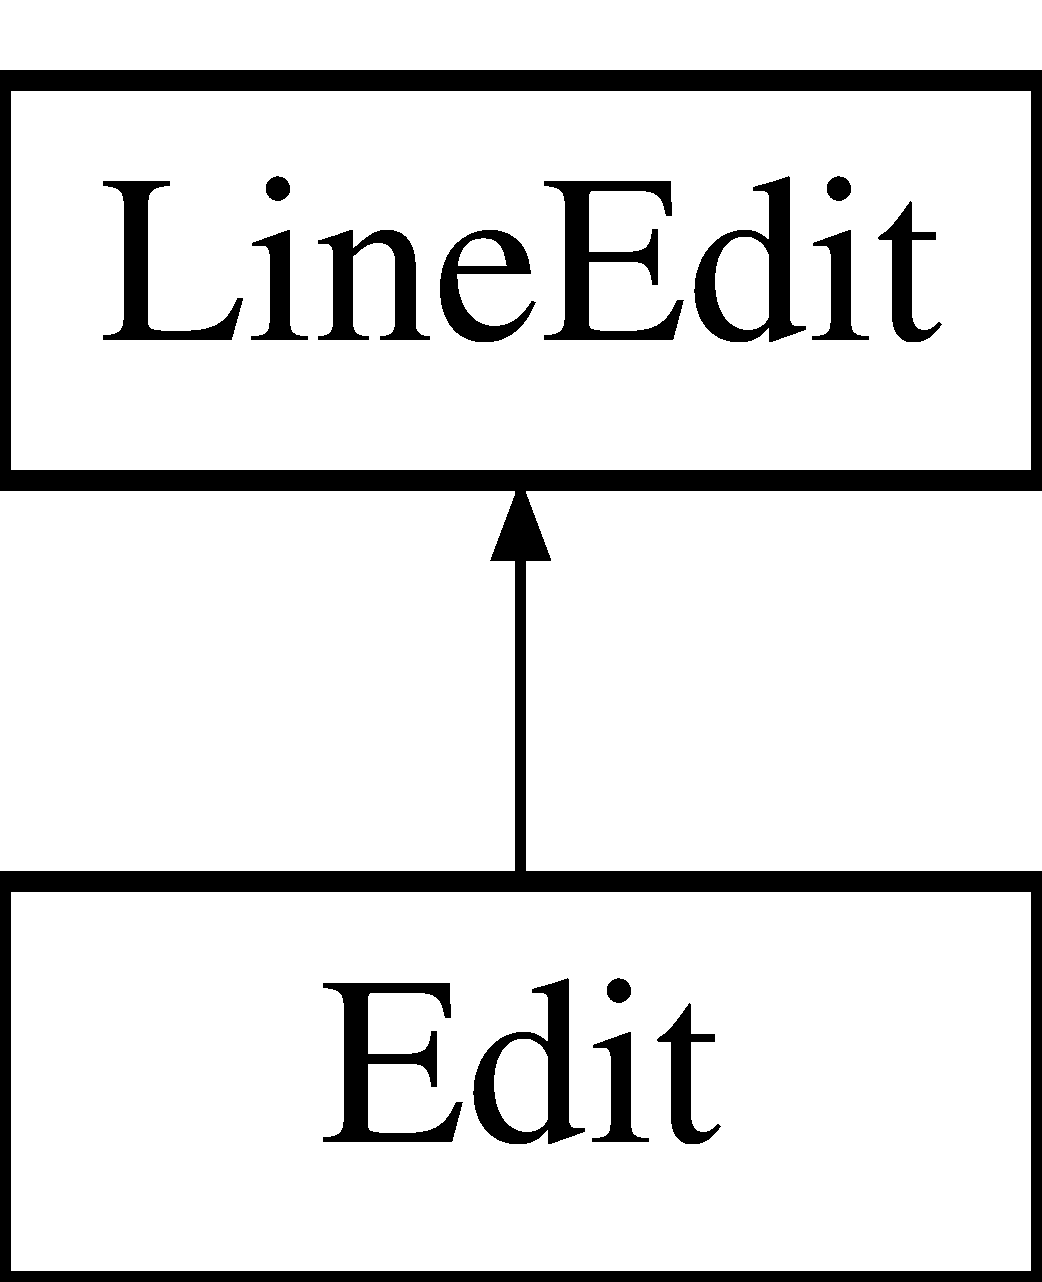
\includegraphics[height=2.000000cm]{classEdit}
\end{center}
\end{figure}
\subsection*{Public Member Functions}
\begin{DoxyCompactItemize}
\item 
\hyperlink{classEdit_ae9f6f3d4ff769401f789e5b71775f55a}{Edit} (QWidget $\ast$parent=0)
\end{DoxyCompactItemize}


\subsection{Detailed Description}


Definition at line 185 of file vwidgets.h.



\subsection{Constructor \& Destructor Documentation}
\hypertarget{classEdit_ae9f6f3d4ff769401f789e5b71775f55a}{
\index{Edit@{Edit}!Edit@{Edit}}
\index{Edit@{Edit}!Edit@{Edit}}
\subsubsection[{Edit}]{\setlength{\rightskip}{0pt plus 5cm}Edit::Edit (
\begin{DoxyParamCaption}
\item[{QWidget $\ast$}]{parent = {\ttfamily 0}}
\end{DoxyParamCaption}
)}}
\label{classEdit_ae9f6f3d4ff769401f789e5b71775f55a}


Definition at line 450 of file vwidgets.cpp.



The documentation for this class was generated from the following files:\begin{DoxyCompactItemize}
\item 
/e/ms/QT/models/\hyperlink{vwidgets_8h}{vwidgets.h}\item 
/e/ms/QT/models/\hyperlink{vwidgets_8cpp}{vwidgets.cpp}\end{DoxyCompactItemize}

\hypertarget{structFgl_1_1Event}{
\section{Fgl::Event Struct Reference}
\label{structFgl_1_1Event}\index{Fgl::Event@{Fgl::Event}}
}


{\ttfamily \#include $<$fgl.h$>$}

\subsection*{Public Attributes}
\begin{DoxyCompactItemize}
\item 
\hyperlink{namespaceFgl_a7bbae69263a5d0012370d5cbb859c6a8}{EventType} \hyperlink{structFgl_1_1Event_afa40f4cb59b82a49e431a4233e77aa37}{type}
\item 
QString \hyperlink{structFgl_1_1Event_a28367efebda5c671dc1e82084e18f0eb}{id}
\item 
QString \hyperlink{structFgl_1_1Event_af77c15903b8674b655c055f686bc0159}{attribute}
\item 
QString \hyperlink{structFgl_1_1Event_a3dc3e7b462f744c1794efffeadc577a8}{field}
\end{DoxyCompactItemize}


\subsection{Detailed Description}


Definition at line 14 of file fgl.h.



\subsection{Member Data Documentation}
\hypertarget{structFgl_1_1Event_af77c15903b8674b655c055f686bc0159}{
\index{Fgl::Event@{Fgl::Event}!attribute@{attribute}}
\index{attribute@{attribute}!Fgl::Event@{Fgl::Event}}
\subsubsection[{attribute}]{\setlength{\rightskip}{0pt plus 5cm}QString {\bf Fgl::Event::attribute}}}
\label{structFgl_1_1Event_af77c15903b8674b655c055f686bc0159}


Definition at line 17 of file fgl.h.

\hypertarget{structFgl_1_1Event_a3dc3e7b462f744c1794efffeadc577a8}{
\index{Fgl::Event@{Fgl::Event}!field@{field}}
\index{field@{field}!Fgl::Event@{Fgl::Event}}
\subsubsection[{field}]{\setlength{\rightskip}{0pt plus 5cm}QString {\bf Fgl::Event::field}}}
\label{structFgl_1_1Event_a3dc3e7b462f744c1794efffeadc577a8}


Definition at line 18 of file fgl.h.

\hypertarget{structFgl_1_1Event_a28367efebda5c671dc1e82084e18f0eb}{
\index{Fgl::Event@{Fgl::Event}!id@{id}}
\index{id@{id}!Fgl::Event@{Fgl::Event}}
\subsubsection[{id}]{\setlength{\rightskip}{0pt plus 5cm}QString {\bf Fgl::Event::id}}}
\label{structFgl_1_1Event_a28367efebda5c671dc1e82084e18f0eb}


Definition at line 16 of file fgl.h.

\hypertarget{structFgl_1_1Event_afa40f4cb59b82a49e431a4233e77aa37}{
\index{Fgl::Event@{Fgl::Event}!type@{type}}
\index{type@{type}!Fgl::Event@{Fgl::Event}}
\subsubsection[{type}]{\setlength{\rightskip}{0pt plus 5cm}{\bf EventType} {\bf Fgl::Event::type}}}
\label{structFgl_1_1Event_afa40f4cb59b82a49e431a4233e77aa37}


Definition at line 15 of file fgl.h.



The documentation for this struct was generated from the following file:\begin{DoxyCompactItemize}
\item 
/e/ms/QT/include/\hyperlink{fgl_8h}{fgl.h}\end{DoxyCompactItemize}

\hypertarget{classFglForm}{
\section{FglForm Class Reference}
\label{classFglForm}\index{FglForm@{FglForm}}
}


{\ttfamily \#include $<$fglform.h$>$}

\subsection*{Public Slots}
\begin{DoxyCompactItemize}
\item 
void \hyperlink{classFglForm_a0ee0e2722721bf18a2809e670e0777cf}{buttonClicked} (QString)
\item 
void \hyperlink{classFglForm_a1fd5cabc8ec447738e4420f618d69ca7}{fieldEvent} (\hyperlink{structFgl_1_1Event}{Fgl::Event}, QWidget $\ast$=NULL)
\item 
void \hyperlink{classFglForm_a763db4c754333829447f9766c25f0e0b}{setBufferTouched} ()
\item 
void \hyperlink{classFglForm_a8495f6c9444756a6bdf370c3ce158921}{setLastCursor} (int, int)
\item 
void \hyperlink{classFglForm_ab61a1af085f68fa6673e516812b0b9c8}{setLastCursor} ()
\item 
void \hyperlink{classFglForm_a7146bdb938bcb9a88b23051b39ea19b7}{setBufferNotTouched} ()
\item 
void \hyperlink{classFglForm_a21cf637edb3ad010d7e00e4d20b95825}{cancelTriggered} ()
\item 
void \hyperlink{classFglForm_afd623938967b4f76707704ab67032a57}{acceptTriggered} ()
\item 
void \hyperlink{classFglForm_a2300cda82ffb223096c19f63004e248f}{accept} ()
\item 
void \hyperlink{classFglForm_a0e2bda025291fc5a29a74254418cffdb}{interrupt} ()
\item 
void \hyperlink{classFglForm_ac51ab1764a0c88802875af3b0ef890af}{editcopy} ()
\item 
void \hyperlink{classFglForm_acba6e2dba68f2d8c8354a1f3e7de0213}{editcut} ()
\item 
void \hyperlink{classFglForm_a3bbc33d5de6401f21553a0e09e091292}{editpaste} ()
\item 
void \hyperlink{classFglForm_a1a279ed4bf3d729f30a346e8e6c9b8c7}{nextfield} (bool change=true)
\item 
void \hyperlink{classFglForm_a1a8413bf151ffd1e9fb4b0ae2a78dd6e}{prevfield} ()
\item 
void \hyperlink{classFglForm_a0321ef0bb745923607aecc90ff23dc16}{nextrow} ()
\item 
void \hyperlink{classFglForm_a92a335499ab7c95fa5b106f7a9f21e33}{prevrow} ()
\item 
void \hyperlink{classFglForm_af18f12d697d5a9fa0041c597d692d8f1}{firstrow} ()
\item 
void \hyperlink{classFglForm_adbc1aae701b9f9be093df1b60072ed10}{lastrow} ()
\item 
void \hyperlink{classFglForm_aafc9f7cacb9852d58b809a840abc104e}{nextpage} ()
\item 
void \hyperlink{classFglForm_ac3cf8e2f5bfc433cb19497e6bad4db0d}{prevpage} ()
\item 
void \hyperlink{classFglForm_a3f1ae54d6ef1585a6f14cf394758c09b}{nexttab} ()
\item 
void \hyperlink{classFglForm_a9eefd50c2b2dbcd9303a20a02a2ad140}{prevtab} ()
\item 
void \hyperlink{classFglForm_ac9689ad22eff52db3ab60446b78274e3}{exitMenu} ()
\item 
void \hyperlink{classFglForm_a267469fbb08f5d257f162df03b88852a}{reopenPulldown} ()
\item 
void \hyperlink{classFglForm_a0ccb7e3f717496c6dceaf34b0a6d49df}{dropSuccess} ()
\item 
void \hyperlink{classFglForm_a2a05aab413be356d8591d9feaa3818ea}{dragSuccess} ()
\item 
void \hyperlink{classFglForm_a6c13e4f1841a38f5cbf615595f88f78f}{sendactivateinputevent} ()
\item 
void \hyperlink{classFglForm_a1d7dad289a4b04321a2c932adf12d19b}{resetFieldSettings} ()
\item 
void \hyperlink{classFglForm_a3d7ccbba13b950e970333db68755d022}{saveFieldSettings} (QAction $\ast$)
\item 
void \hyperlink{classFglForm_a4430f1038e2dcfd957c1d361d0c286d4}{clearCurrentFocus} ()
\item 
void \hyperlink{classFglForm_ae2815f84a3c114c000f97cc0cf431bb7}{clearFieldFocus} ()
\item 
void \hyperlink{classFglForm_abacf589f219bcfbcf54ca2a5fb9ba859}{setFocusOnWidget} (QWidget $\ast$, Qt::FocusReason=Qt::OtherFocusReason)
\begin{DoxyCompactList}\small\item\em Method to set Focus and remove the focus of all other widgets. \item\end{DoxyCompactList}\item 
void \hyperlink{classFglForm_a5e7fe57471d1f3ad4d6dbf7ac1c8b843}{sendMenuCommand} (QString)
\item 
void \hyperlink{classFglForm_af3d272e5dc101746b728bdd457d42a6f}{setStartMenu} (const QDomDocument \&doc)
\item 
void \hyperlink{classFglForm_af07f7257121ab71b9a53ccb2fd1a9fe3}{createContextMenu} (const QPoint \&)
\item 
void \hyperlink{classFglForm_afce8d989187c85d7bde751824a9b6c6a}{setScreenRecordArrLine} (int)
\item 
void \hyperlink{classFglForm_a3d2c6f2a3a0e1828ff1f43d4d93fa775}{error} (const QString \&)
\item 
void \hyperlink{classFglForm_a95fd29ee66dc40bb56d6bb94593feddd}{checkField} ()
\item 
void \hyperlink{classFglForm_a4fdd15cf1295a7d04b378e5c4cb2d877}{writeSettingsLocal} ()
\item 
void \hyperlink{classFglForm_ae9f393760ac910dd86de0919be07f41c}{readSettingsLocal} ()
\end{DoxyCompactItemize}
\subsection*{Signals}
\begin{DoxyCompactItemize}
\item 
void \hyperlink{classFglForm_a797f5a3e960a73a6fff9a1bb74059956}{processResponse} ()
\item 
void \hyperlink{classFglForm_ab8e58a4d027770ba170972d247b617dd}{sendDirect} (QString)
\item 
void \hyperlink{classFglForm_a1e972cdb1514dcb3c6613d123beb8f6a}{accepted} ()
\item 
void \hyperlink{classFglForm_a9c7de4f0bd6f44e3103df2e81a504974}{setClearEvents} ()
\item 
void \hyperlink{classFglForm_a7bef8f5a9e151e3b09d9de652b78ec92}{setArrLine} (int)
\item 
void \hyperlink{classFglForm_a6084470ee7bb46645d64a82503c60fba}{closeAction} ()
\end{DoxyCompactItemize}
\subsection*{Public Member Functions}
\begin{DoxyCompactItemize}
\item 
\hyperlink{classFglForm_a4a6d10fc6cce5a7984d59b80730cd7e1}{FglForm} (QString \hyperlink{classFglForm_a154084978ed81b8739db7197541881f5}{windowName}=\char`\"{}\char`\"{}, QWidget $\ast$parent=0)
\begin{DoxyCompactList}\small\item\em Constructor for the Fglform. \item\end{DoxyCompactList}\item 
\hyperlink{classFglForm_a14fc02c52beeeffefa92a4b3425da772}{$\sim$FglForm} ()
\item 
void \hyperlink{classFglForm_a626014edfd45271d30f38d877601abd5}{jumpToField} (QWidget $\ast$, bool b\_\-after=true)
\item 
void \hyperlink{classFglForm_acfb920aa37d488d2877fe75441ac7f65}{setMenuEnabled} (bool)
\item 
void \hyperlink{classFglForm_a0060da33eb1943f1b762e8a164ede398}{setMenu} (\hyperlink{classRingMenu}{RingMenu} $\ast$)
\item 
void \hyperlink{classFglForm_a7b0af358781bf6b0f37d80e9383cf10e}{removeMenu} ()
\item 
\hyperlink{classRingMenu}{RingMenu} $\ast$ \hyperlink{classFglForm_acffbcaf62fc53ff47363cf13b2967242}{menu} ()
\item 
void \hyperlink{classFglForm_ab322288b13021e7b98a5cf87912d2f18}{setActionMenuEnabled} (bool)
\item 
void \hyperlink{classFglForm_acdc54b976403abededb061ba2dd0c30f}{setActionMenu} (\hyperlink{classActionMenu}{ActionMenu} $\ast$)
\item 
\hyperlink{classActionMenu}{ActionMenu} $\ast$ \hyperlink{classFglForm_aa7339ffc3aa81015c493104643fde6a1}{actionMenu} ()
\item 
void \hyperlink{classFglForm_aee2921f4bcb8f95e10fde25ec84842d3}{setDialog} (\hyperlink{classDialog}{Dialog} $\ast$)
\item 
void \hyperlink{classFglForm_a19892721571e2c56399ca6be07c3f750}{setPulldown} (\hyperlink{classPulldown}{Pulldown} $\ast$)
\item 
\hyperlink{classDialog}{Dialog} $\ast$ \hyperlink{classFglForm_ace102516f1523e1ea87c64f2db1ea30e}{dialog} ()
\item 
\hyperlink{classPulldown}{Pulldown} $\ast$ \hyperlink{classFglForm_a05f163612a936468e8fac3e84aeec02e}{pulldown} ()
\item 
void \hyperlink{classFglForm_a81b6a444e67df3a3e56ff786fe9099b7}{showEvent} (QShowEvent $\ast$)
\item 
void \hyperlink{classFglForm_acf0280c2e7ca7d56bc45c822b8fb9468}{setToolBar} (\hyperlink{classToolBar}{ToolBar} $\ast$)
\item 
void \hyperlink{classFglForm_ad139148f573546a3ef5ead0f49170d08}{setToolBar} (QDomDocument)
\item 
void \hyperlink{classFglForm_a7490e381d17c7644c7f37a58d5ffa9b4}{checkToolBar} ()
\item 
void \hyperlink{classFglForm_ab7d3ed99ee7eac4b6b781e576d33a1ea}{checkMenu} ()
\item 
ScreenHandler $\ast$ \hyperlink{classFglForm_aebb86e0bc590b730ff490b030b5dba7c}{screenhandler} ()
\item 
void \hyperlink{classFglForm_aba5859f32918808eb18606b85483a4c6}{setScreenHandler} (ScreenHandler $\ast$)
\item 
void \hyperlink{classFglForm_ad806af9cecf975dc4abe1e12eb52864a}{checkActions} ()
\item 
void \hyperlink{classFglForm_a3770f9b34c38cb5bc3f66a7e388c43ce}{checkShortcuts} ()
\item 
void \hyperlink{classFglForm_a60718980fe99888336db588976319382}{checkGuiActions} ()
\item 
bool \hyperlink{classFglForm_ab44742db0c6d0d2e0663db22c9668b4c}{handleGuiAction} (\hyperlink{classAction}{Action} $\ast$)
\item 
\hyperlink{classToolBar}{ToolBar} $\ast$ \hyperlink{classFglForm_ae474767d66111cda958e191e6be1e34d}{toolBar} ()
\item 
Qt::ToolBarArea \hyperlink{classFglForm_acca25b6cbf4161c7075fb594a556eb9a}{toolBarPosition} ()
\item 
void \hyperlink{classFglForm_a4b9c2e9963530fba9dc68f9dae0928a0}{setActions} (QDomDocument)
\item 
QList$<$ \hyperlink{classAction}{Action} $\ast$ $>$ \hyperlink{classFglForm_ac8a66ae6b84ca24c622a87eb631a4834}{formActions} ()
\item 
QList$<$ \hyperlink{classAction}{Action} $\ast$ $>$ \hyperlink{classFglForm_a1a92c94c67dd0ff9d8ff48c3fc64dcf9}{defActions} ()
\item 
QList$<$ \hyperlink{classAction}{Action} $\ast$ $>$ \hyperlink{classFglForm_aa65ef0a575b40217c5fbbe71c6faaf28}{actionDefaults} ()
\item 
void \hyperlink{classFglForm_ac43c7da12a298a241c7c98cf9a688a6f}{addFormAction} (QAction $\ast$)
\item 
void \hyperlink{classFglForm_a21e61578024f5922c949b4c2870684d4}{addFormAction} (QString name, QString text=\char`\"{}\char`\"{}, QString comment=\char`\"{}\char`\"{}, QString image=\char`\"{}\char`\"{}, QString accName=\char`\"{}\char`\"{}, QString accName2=\char`\"{}\char`\"{}, QString accName3=\char`\"{}\char`\"{}, QString accName4=\char`\"{}\char`\"{}, QString defaultView=\char`\"{}\char`\"{})
\item 
void \hyperlink{classFglForm_abadbd33d56f9bc46b3421f8fe0628952}{addFormEvent} (\hyperlink{structFgl_1_1Event}{Fgl::Event})
\item 
void \hyperlink{classFglForm_a5f3fea57cf46e7d548912efdaffa35f9}{focusNextField} ()
\item 
QWidget $\ast$ \hyperlink{classFglForm_a74cb6310512352e1fd501efbcd88724b}{currentField} ()
\item 
void \hyperlink{classFglForm_ac521356370affcf115340e2279475c6b}{setCurrentWidget} (QWidget $\ast$)
\item 
void \hyperlink{classFglForm_a4574756e714c6d93e6d177ecbfb78ae1}{setCurrentField} (QString, bool sendEvents=true)
\item 
void \hyperlink{classFglForm_a82a066a47d5d8bc2f7c2ec41ab29d4f2}{addToQueue} (\hyperlink{structFgl_1_1Event}{Fgl::Event})
\item 
void \hyperlink{classFglForm_a21e6b7f851487d6d0db29b015a37e374}{addToQueue} (QList$<$ \hyperlink{structFgl_1_1Event}{Fgl::Event} $>$)
\item 
bool \hyperlink{classFglForm_ab6b474ce22c93c45ccbee4b637647732}{input} ()
\item 
bool \hyperlink{classFglForm_ab131183405b70a2d48643ec9a522f877}{construct} ()
\item 
bool \hyperlink{classFglForm_a2e45f9d338ef208ffb1c08f1f97e6b2b}{screenRecord} ()
\item 
bool \hyperlink{classFglForm_a77b1a70cf1fff7d103b8c1895b3302c4}{displayArray} ()
\item 
bool \hyperlink{classFglForm_a452b19a215f6acbb86320ed3a8b32ead}{inputArray} ()
\item 
bool \hyperlink{classFglForm_ae6cab599f897bf58335df99e6d43b72d}{bufferTouched} ()
\item 
int \hyperlink{classFglForm_aab860a48ab46e95732543f3cb345ba26}{lastCursor} ()
\item 
void \hyperlink{classFglForm_af5e8206054e3275e2977056e685b73da}{initActions} ()
\item 
void \hyperlink{classFglForm_a6a923c50e859e58d34046d0b0f86c11d}{setFormLayout} (const QDomDocument \&)
\item 
void \hyperlink{classFglForm_a07c0926396e4229b40de7988689a1f16}{setStyles} (const QDomDocument \&)
\item 
QString \hyperlink{classFglForm_a40002405b99f9291e8f61944a775172a}{getStartMenuPosition} () const 
\item 
void \hyperlink{classFglForm_a2badc0486f40c57306fdefe14800a13b}{setStartMenuPosition} (const QString \&sm)
\item 
QString \hyperlink{classFglForm_ac138a537d43b85e677818e1a61f3cd3d}{getToolBarPosition} () const 
\item 
void \hyperlink{classFglForm_af3b00991b1e002fe156d0298468a2311}{setToolBarPosition} (const QString \&sm)
\item 
QString \hyperlink{classFglForm_a1e47b1b987a50ed9e4155bdf0664feba}{getWindowType} () const 
\item 
void \hyperlink{classFglForm_ad780eff8bf0437a8e33a9115885718e9}{setWindowType} (const QString \&sm)
\item 
QString \hyperlink{classFglForm_a714fbe1dca04c76d368a8a429b6322c1}{sizable} () const 
\item 
void \hyperlink{classFglForm_a805e33b8b74b0cc73dad05eac238f9db}{setSizable} (const QString \&sm)
\item 
bool \hyperlink{classFglForm_a9cacfea35fa0152d42b399fc6d2a2524}{getDefaultStatusBar} () const 
\item 
void \hyperlink{classFglForm_a4b2f8754ef3aa90fc46d04c2020ed5af}{setDefaultStatusBar} (const bool \&sm)
\item 
QString \hyperlink{classFglForm_a1d53398b0bf7a81f7d6f4fab65faa3dd}{getActionPanelPosition} () const 
\item 
void \hyperlink{classFglForm_a80b78ad88d0dc22b7f4df7a724794a13}{setActionPanelPosition} (const QString \&sm)
\item 
QString \hyperlink{classFglForm_a773cd80cab1ae1efaccc48262b2cbc55}{getRingMenuPosition} () const 
\item 
void \hyperlink{classFglForm_af25c944e246c0522cd333e452ead9cad}{setRingMenuPosition} (const QString \&sm)
\item 
void \hyperlink{classFglForm_a5f6285fdf157e863c68402ec8147c53a}{setState} (\hyperlink{namespaceFgl_a66700792cb225549384ae76c1057cf22}{Fgl::State} state)
\item 
void \hyperlink{classFglForm_a4d2edce15aac96b22d221a11c0e7681e}{revertState} (\hyperlink{namespaceFgl_a66700792cb225549384ae76c1057cf22}{Fgl::State})
\item 
\hyperlink{namespaceFgl_a66700792cb225549384ae76c1057cf22}{Fgl::State} \hyperlink{classFglForm_aeed42adf5a051006db1742e2b48617e1}{state} ()
\item 
void \hyperlink{classFglForm_a0ef6e6d0ddf327e89c3e2d54be8548a6}{checkState} ()
\item 
QList$<$ QWidget $\ast$ $>$ \hyperlink{classFglForm_ab40c533416d35aac75f2ccf5157a3cf2}{formElements} ()
\item 
QWidget $\ast$ \hyperlink{classFglForm_a7490b2d18830368110a69983f19d65cf}{findFieldByName} (QString)
\item 
QList$<$ QWidget $\ast$ $>$ \hyperlink{classFglForm_aa9bed6529e8937fdf1ebed65ca23cc45}{findFieldsByName} (QString)
\item 
int \hyperlink{classFglForm_a4d506d1f05b8ac540fe33dfa1524d681}{findFieldIdByName} (QString)
\item 
QWidget $\ast$ \hyperlink{classFglForm_a997cd55b341e14c89fdc300efe75b907}{findFieldById} (int)
\item 
void \hyperlink{classFglForm_a7010467be800cf868884b589f8ce8ce7}{setId} (QString id)
\item 
int \hyperlink{classFglForm_a4fc9bc745910f209c6f54f509293bd73}{id} ()
\item 
void \hyperlink{classFglForm_a47d0bbf071cbf0051b72c44a90062f81}{setUserInputEnabled} (bool enabled)
\end{DoxyCompactItemize}
\subsection*{Public Attributes}
\begin{DoxyCompactItemize}
\item 
bool \hyperlink{classFglForm_a8c411d93b67981a684a5cf6b67111dc1}{b\_\-svs}
\item 
QString \hyperlink{classFglForm_a154084978ed81b8739db7197541881f5}{windowName}
\item 
QWidget $\ast$ \hyperlink{classFglForm_abce220040f982717756bfc10b51dac44}{currentWidget}
\item 
QPointer$<$ QPushButton $>$ \hyperlink{classFglForm_a17945f68955698f41dac6b11cf73cd07}{nextclick}
\item 
bool \hyperlink{classFglForm_ac6325d19f253fe4e7cdfbd50bd027c19}{b\_\-getch\_\-swin}
\item 
bool \hyperlink{classFglForm_af7e3a4c11559a83dd68df64c286fdb1e}{b\_\-allowClose}
\item 
bool \hyperlink{classFglForm_a4dd283ca13e8a699e88783b2946b6841}{b\_\-dummy}
\item 
QList$<$ \hyperlink{structFgl_1_1Event}{Fgl::Event} $>$ \hyperlink{classFglForm_a3aa184c0556d81cfb244f726d95b0538}{ql\_\-responseQueue}
\item 
QStringList \hyperlink{classFglForm_ab53b016e506ad4ed7fdb2ac2210d43b1}{qsl\_\-fieldOrder}
\item 
QHash$<$ QString, QList$<$ \hyperlink{structFgl_1_1Link}{Fgl::Link} $>$ $>$ \hyperlink{classFglForm_a2e8895a4cd6f58cc36f31c8a51c06a54}{recordView}
\item 
bool \hyperlink{classFglForm_ab089d04abad8973c262e3c5e1827b070}{b\_\-newForm}
\item 
bool \hyperlink{classFglForm_a99b822401e45535d412f2a6c5601734d}{b\_\-denyFocus}
\item 
int \hyperlink{classFglForm_a34347fff01950e4574b64c69b62d1ff2}{gridWidth}
\item 
QList$<$ \hyperlink{structFgl_1_1Event}{Fgl::Event} $>$ \hyperlink{classFglForm_a0a20950e5d9deba35525fbcb7935f6f0}{ql\_\-menuEvents}
\item 
QList$<$ \hyperlink{structFgl_1_1Event}{Fgl::Event} $>$ \hyperlink{classFglForm_a764e11f62e1849d568cda143fa11583e}{ql\_\-dialogEvents}
\item 
QList$<$ \hyperlink{structFgl_1_1Event}{Fgl::Event} $>$ \hyperlink{classFglForm_a14b1e58865612b4ebbfa83c8769f9353}{ql\_\-pulldownEvents}
\item 
QList$<$ \hyperlink{structFgl_1_1Event}{Fgl::Event} $>$ \hyperlink{classFglForm_aec60babfa521575768a4aa1147318ba1}{ql\_\-formEvents}
\item 
QList$<$ QList$<$ \hyperlink{structFgl_1_1Event}{Fgl::Event} $>$ $>$ \hyperlink{classFglForm_ac7920cda2f9ebef4076ff19e73cfa047}{ql\_\-contextEvents}
\item 
QList$<$ QWidget $\ast$ $>$ \hyperlink{classFglForm_ad0adbaabeb97d6fabd2a23f5ac5c0069}{ql\_\-formFields}
\item 
QStringList \hyperlink{classFglForm_a127a846458930510880fd13eb07d4463}{qsl\_\-activeFields}
\item 
Context $\ast$ \hyperlink{classFglForm_ad88a7b19b295fe1f14de652a9e3e1c17}{context}
\end{DoxyCompactItemize}
\subsection*{Protected Member Functions}
\begin{DoxyCompactItemize}
\item 
bool \hyperlink{classFglForm_ad684c111c48ae9b6bfee70f36383e8a0}{eventFilter} (QObject $\ast$obj, QEvent $\ast$event)
\item 
void \hyperlink{classFglForm_ab4a2e829699bf5c49124801ccd0eb5f2}{closeEvent} (QCloseEvent $\ast$event)
\item 
void \hyperlink{classFglForm_a039e7ba89ece4f1bb47c32dc34271536}{contextMenuEvent} (QContextMenuEvent $\ast$)
\item 
bool \hyperlink{classFglForm_abbb79e3d5fbc48341d4e88bc91002c22}{focusNextPrevChild} (bool)
\end{DoxyCompactItemize}
\subsection*{Properties}
\begin{DoxyCompactItemize}
\item 
QString \hyperlink{classFglForm_a5262a92dfdf82913701d4661bbefaaac}{windowType}
\item 
QString \hyperlink{classFglForm_aec7035cbd1e5a013f2d96a1a3a98aa53}{startMenuPosition}
\item 
QString \hyperlink{classFglForm_a2e26a9f76fe7c63c8103ac4b04776e81}{sizable}
\item 
bool \hyperlink{classFglForm_aed179664fb0f0999affabd3b746edae7}{defaultStatusBar}
\item 
QString \hyperlink{classFglForm_afc1641787bae0be3864cce6efdea9e17}{toolBarPosition}
\item 
QString \hyperlink{classFglForm_a8ca117823135914a8977974b455372a1}{actionPanelPosition}
\item 
QString \hyperlink{classFglForm_ab0e939affc05fa6c0297dcf7c257b25f}{ringMenuPosition}
\end{DoxyCompactItemize}
\subsection*{Private Slots}
\begin{DoxyCompactItemize}
\item 
void \hyperlink{classFglForm_a6a62cd6e46c191cbec6c49381fd53a95}{actionTriggered} ()
\item 
void \hyperlink{classFglForm_a7d6b1d8b49f56f8b8ae6dbffae4a6499}{toolBarActionTriggered} ()
\end{DoxyCompactItemize}
\subsection*{Private Member Functions}
\begin{DoxyCompactItemize}
\item 
void \hyperlink{classFglForm_a98a3ed85a0f12181c96d15a020250807}{createStatusBar} ()
\end{DoxyCompactItemize}
\subsection*{Private Attributes}
\begin{DoxyCompactItemize}
\item 
e ms QT models fglform \hyperlink{classFglForm_a2adf651bccc4bd01a985a0c5bde45af7}{h} e ms QT models fglform \hyperlink{classFglForm_a2adf651bccc4bd01a985a0c5bde45af7}{h} e ms QT models fglform \hyperlink{classFglForm_a2adf651bccc4bd01a985a0c5bde45af7}{h} e ms QT models fglform \hyperlink{classFglForm_a2adf651bccc4bd01a985a0c5bde45af7}{h} e ms QT models fglform \hyperlink{classFglForm_a2adf651bccc4bd01a985a0c5bde45af7}{h}
\item 
QList$<$ \hyperlink{namespaceFgl_a66700792cb225549384ae76c1057cf22}{Fgl::State} $>$ \hyperlink{classFglForm_a18774054d5c9773a7075b5933b0bbc9a}{ql\_\-states}
\item 
QWidget $\ast$ \hyperlink{classFglForm_a382565fe4e148f5e37aabea41e079809}{formWidget}
\item 
QList$<$ \hyperlink{classRingMenu}{RingMenu} $\ast$ $>$ \hyperlink{classFglForm_a587196a08706e03ec05f1fae4048f344}{ql\_\-menus}
\item 
QPointer$<$ ScreenHandler $>$ \hyperlink{classFglForm_a98e11b2d55100f907821e3a8281b4ab5}{p\_\-currscreenhandler}
\item 
\hyperlink{classActionMenu}{ActionMenu} $\ast$ \hyperlink{classFglForm_aace1d4f7b637af4d3aa86e53a770152e}{p\_\-actionMenu}
\item 
\hyperlink{classDialog}{Dialog} $\ast$ \hyperlink{classFglForm_afa28d86c6e353e3e31c677b463199a4a}{p\_\-dialog}
\item 
\hyperlink{classPulldown}{Pulldown} $\ast$ \hyperlink{classFglForm_a87a0ac69973f45c48fb629d04ac5b364}{p\_\-pulldown}
\item 
\hyperlink{classToolBar}{ToolBar} $\ast$ \hyperlink{classFglForm_a63ee680575b50bd02473649cd3d272f5}{p\_\-toolBar}
\item 
QAction $\ast$ \hyperlink{classFglForm_ac85748725f2a9ba437e62be1293eae02}{rightAct}
\item 
QAction $\ast$ \hyperlink{classFglForm_aa9bb2c29fa0161164dd5250a7602a1be}{resetAct}
\item 
QList$<$ \hyperlink{classAction}{Action} $\ast$ $>$ \hyperlink{classFglForm_a091b50c03ba4a353485d34ea34f4001a}{ql\_\-formActions}
\item 
QList$<$ \hyperlink{classAction}{Action} $\ast$ $>$ \hyperlink{classFglForm_acc7f6b6c7b13cf1e6e39bfdeba18ddc1}{ql\_\-defaultActions}
\item 
QList$<$ \hyperlink{classAction}{Action} $\ast$ $>$ \hyperlink{classFglForm_a6b78dae39bcab3791a9acc99a3b8248d}{ql\_\-actionDefaults}
\item 
QList$<$ \hyperlink{classFormField}{FormField} $\ast$ $>$ \hyperlink{classFglForm_a1d775e481b65ae50b2a557fa9ae975c5}{ql\_\-fglFields}
\item 
bool \hyperlink{classFglForm_ac1f8bea18516701b1192825f83e962d7}{b\_\-menu}
\item 
bool \hyperlink{classFglForm_a348ba4d61a2c9e18513ac88c919015c0}{b\_\-input}
\item 
bool \hyperlink{classFglForm_a656061ca98f40226c99fa61b12ced56c}{b\_\-screenRecord}
\item 
QString \hyperlink{classFglForm_aff3b675ee7063af63839e029f66b4075}{m\_\-windowType}
\item 
QString \hyperlink{classFglForm_a94e20a9c06c349d6e7c5ec47c03de4a6}{m\_\-startMenuPosition}
\item 
QString \hyperlink{classFglForm_a0008c6a1c3362095ebd5ab0601910003}{m\_\-toolBarPosition}
\item 
QString \hyperlink{classFglForm_a25371a3df6cb3e1dc66e141bb2a9dff1}{m\_\-ringMenuPosition}
\item 
QString \hyperlink{classFglForm_af3882d981d23db8e6dca26a44ac23051}{m\_\-actionPanelPosition}
\item 
QString \hyperlink{classFglForm_a7861c07caeb306c5ae9f2012ce73bff7}{m\_\-sizable}
\item 
bool \hyperlink{classFglForm_a2e877386e4ba441d929c0c35d48620cb}{m\_\-defaultStatusBar}
\item 
QWidget $\ast$ \hyperlink{classFglForm_a15cd139d56b40da6de43a6bb4d438c0d}{widget}
\item 
QLabel $\ast$ \hyperlink{classFglForm_a72467aa7c8750f7075b7ba7fc67a29bb}{insLabel}
\item 
int \hyperlink{classFglForm_ae7e903902c63ce3179656df4b684038f}{i\_\-currentField}
\item 
QWidget $\ast$ \hyperlink{classFglForm_a67c8174c2d61e69e76c3206766fe3ac9}{fieldsContainer}
\item 
int \hyperlink{classFglForm_a6142cd4363f16562e52631f1987b46c3}{i\_\-id}
\item 
bool \hyperlink{classFglForm_a4bddddc3ca57303fbf3d55394e260a00}{b\_\-bufferTouched}
\item 
int \hyperlink{classFglForm_a9f622b4a17fcad8c785e119d19abe326}{i\_\-lastCursor}
\item 
QString \hyperlink{classFglForm_a04725912842355fc88fa7412e435f4a9}{qs\_\-currentFieldBuffer}
\item 
QString \hyperlink{classFglForm_a1bca5dcb62f50a5939c295b7c0d662d2}{qs\_\-formfile}
\item 
int \hyperlink{classFglForm_a9dc5de78bd4b0d7024831926f9cdc7d9}{gridHeight}
\end{DoxyCompactItemize}


\subsection{Detailed Description}


Definition at line 42 of file fglform.h.



\subsection{Constructor \& Destructor Documentation}
\hypertarget{classFglForm_a4a6d10fc6cce5a7984d59b80730cd7e1}{
\index{FglForm@{FglForm}!FglForm@{FglForm}}
\index{FglForm@{FglForm}!FglForm@{FglForm}}
\subsubsection[{FglForm}]{\setlength{\rightskip}{0pt plus 5cm}FglForm::FglForm (
\begin{DoxyParamCaption}
\item[{QString}]{windowName = {\ttfamily \char`\"{}\char`\"{}}, }
\item[{QWidget $\ast$}]{parent = {\ttfamily 0}}
\end{DoxyParamCaption}
)}}
\label{classFglForm_a4a6d10fc6cce5a7984d59b80730cd7e1}


Constructor for the Fglform. 



Definition at line 39 of file fglform.cpp.

\hypertarget{classFglForm_a14fc02c52beeeffefa92a4b3425da772}{
\index{FglForm@{FglForm}!$\sim$FglForm@{$\sim$FglForm}}
\index{$\sim$FglForm@{$\sim$FglForm}!FglForm@{FglForm}}
\subsubsection[{$\sim$FglForm}]{\setlength{\rightskip}{0pt plus 5cm}FglForm::$\sim$FglForm (
\begin{DoxyParamCaption}
{}
\end{DoxyParamCaption}
)}}
\label{classFglForm_a14fc02c52beeeffefa92a4b3425da772}


Definition at line 114 of file fglform.cpp.



\subsection{Member Function Documentation}
\hypertarget{classFglForm_a2300cda82ffb223096c19f63004e248f}{
\index{FglForm@{FglForm}!accept@{accept}}
\index{accept@{accept}!FglForm@{FglForm}}
\subsubsection[{accept}]{\setlength{\rightskip}{0pt plus 5cm}void FglForm::accept (
\begin{DoxyParamCaption}
{}
\end{DoxyParamCaption}
)\hspace{0.3cm}{\ttfamily  \mbox{[}slot\mbox{]}}}}
\label{classFglForm_a2300cda82ffb223096c19f63004e248f}


Definition at line 1512 of file fglform.cpp.

\hypertarget{classFglForm_a1e972cdb1514dcb3c6613d123beb8f6a}{
\index{FglForm@{FglForm}!accepted@{accepted}}
\index{accepted@{accepted}!FglForm@{FglForm}}
\subsubsection[{accepted}]{\setlength{\rightskip}{0pt plus 5cm}void FglForm::accepted (
\begin{DoxyParamCaption}
{}
\end{DoxyParamCaption}
)\hspace{0.3cm}{\ttfamily  \mbox{[}signal\mbox{]}}}}
\label{classFglForm_a1e972cdb1514dcb3c6613d123beb8f6a}
\hypertarget{classFglForm_afd623938967b4f76707704ab67032a57}{
\index{FglForm@{FglForm}!acceptTriggered@{acceptTriggered}}
\index{acceptTriggered@{acceptTriggered}!FglForm@{FglForm}}
\subsubsection[{acceptTriggered}]{\setlength{\rightskip}{0pt plus 5cm}void FglForm::acceptTriggered (
\begin{DoxyParamCaption}
{}
\end{DoxyParamCaption}
)\hspace{0.3cm}{\ttfamily  \mbox{[}slot\mbox{]}}}}
\label{classFglForm_afd623938967b4f76707704ab67032a57}


Definition at line 1484 of file fglform.cpp.

\hypertarget{classFglForm_aa65ef0a575b40217c5fbbe71c6faaf28}{
\index{FglForm@{FglForm}!actionDefaults@{actionDefaults}}
\index{actionDefaults@{actionDefaults}!FglForm@{FglForm}}
\subsubsection[{actionDefaults}]{\setlength{\rightskip}{0pt plus 5cm}QList$<${\bf Action}$\ast$$>$ FglForm::actionDefaults (
\begin{DoxyParamCaption}
{}
\end{DoxyParamCaption}
)\hspace{0.3cm}{\ttfamily  \mbox{[}inline\mbox{]}}}}
\label{classFglForm_aa65ef0a575b40217c5fbbe71c6faaf28}


Definition at line 127 of file fglform.h.

\hypertarget{classFglForm_aa7339ffc3aa81015c493104643fde6a1}{
\index{FglForm@{FglForm}!actionMenu@{actionMenu}}
\index{actionMenu@{actionMenu}!FglForm@{FglForm}}
\subsubsection[{actionMenu}]{\setlength{\rightskip}{0pt plus 5cm}{\bf ActionMenu}$\ast$ FglForm::actionMenu (
\begin{DoxyParamCaption}
{}
\end{DoxyParamCaption}
)\hspace{0.3cm}{\ttfamily  \mbox{[}inline\mbox{]}}}}
\label{classFglForm_aa7339ffc3aa81015c493104643fde6a1}


Definition at line 106 of file fglform.h.

\hypertarget{classFglForm_a6a62cd6e46c191cbec6c49381fd53a95}{
\index{FglForm@{FglForm}!actionTriggered@{actionTriggered}}
\index{actionTriggered@{actionTriggered}!FglForm@{FglForm}}
\subsubsection[{actionTriggered}]{\setlength{\rightskip}{0pt plus 5cm}void FglForm::actionTriggered (
\begin{DoxyParamCaption}
{}
\end{DoxyParamCaption}
)\hspace{0.3cm}{\ttfamily  \mbox{[}private, slot\mbox{]}}}}
\label{classFglForm_a6a62cd6e46c191cbec6c49381fd53a95}


Definition at line 499 of file fglform.cpp.

\hypertarget{classFglForm_ac43c7da12a298a241c7c98cf9a688a6f}{
\index{FglForm@{FglForm}!addFormAction@{addFormAction}}
\index{addFormAction@{addFormAction}!FglForm@{FglForm}}
\subsubsection[{addFormAction}]{\setlength{\rightskip}{0pt plus 5cm}void FglForm::addFormAction (
\begin{DoxyParamCaption}
\item[{QAction $\ast$}]{qaction}
\end{DoxyParamCaption}
)}}
\label{classFglForm_ac43c7da12a298a241c7c98cf9a688a6f}


Definition at line 3030 of file fglform.cpp.

\hypertarget{classFglForm_a21e61578024f5922c949b4c2870684d4}{
\index{FglForm@{FglForm}!addFormAction@{addFormAction}}
\index{addFormAction@{addFormAction}!FglForm@{FglForm}}
\subsubsection[{addFormAction}]{\setlength{\rightskip}{0pt plus 5cm}void FglForm::addFormAction (
\begin{DoxyParamCaption}
\item[{QString}]{name, }
\item[{QString}]{text = {\ttfamily \char`\"{}\char`\"{}}, }
\item[{QString}]{comment = {\ttfamily \char`\"{}\char`\"{}}, }
\item[{QString}]{image = {\ttfamily \char`\"{}\char`\"{}}, }
\item[{QString}]{accName = {\ttfamily \char`\"{}\char`\"{}}, }
\item[{QString}]{accName2 = {\ttfamily \char`\"{}\char`\"{}}, }
\item[{QString}]{accName3 = {\ttfamily \char`\"{}\char`\"{}}, }
\item[{QString}]{accName4 = {\ttfamily \char`\"{}\char`\"{}}, }
\item[{QString}]{defaultView = {\ttfamily \char`\"{}\char`\"{}}}
\end{DoxyParamCaption}
)}}
\label{classFglForm_a21e61578024f5922c949b4c2870684d4}


Definition at line 3082 of file fglform.cpp.

\hypertarget{classFglForm_abadbd33d56f9bc46b3421f8fe0628952}{
\index{FglForm@{FglForm}!addFormEvent@{addFormEvent}}
\index{addFormEvent@{addFormEvent}!FglForm@{FglForm}}
\subsubsection[{addFormEvent}]{\setlength{\rightskip}{0pt plus 5cm}void FglForm::addFormEvent (
\begin{DoxyParamCaption}
\item[{{\bf Fgl::Event}}]{newEvent}
\end{DoxyParamCaption}
)}}
\label{classFglForm_abadbd33d56f9bc46b3421f8fe0628952}


Definition at line 3133 of file fglform.cpp.

\hypertarget{classFglForm_a82a066a47d5d8bc2f7c2ec41ab29d4f2}{
\index{FglForm@{FglForm}!addToQueue@{addToQueue}}
\index{addToQueue@{addToQueue}!FglForm@{FglForm}}
\subsubsection[{addToQueue}]{\setlength{\rightskip}{0pt plus 5cm}void FglForm::addToQueue (
\begin{DoxyParamCaption}
\item[{{\bf Fgl::Event}}]{id}
\end{DoxyParamCaption}
)}}
\label{classFglForm_a82a066a47d5d8bc2f7c2ec41ab29d4f2}


Definition at line 174 of file fglform.cpp.

\hypertarget{classFglForm_a21e6b7f851487d6d0db29b015a37e374}{
\index{FglForm@{FglForm}!addToQueue@{addToQueue}}
\index{addToQueue@{addToQueue}!FglForm@{FglForm}}
\subsubsection[{addToQueue}]{\setlength{\rightskip}{0pt plus 5cm}void FglForm::addToQueue (
\begin{DoxyParamCaption}
\item[{QList$<$ {\bf Fgl::Event} $>$}]{events}
\end{DoxyParamCaption}
)}}
\label{classFglForm_a21e6b7f851487d6d0db29b015a37e374}


Definition at line 182 of file fglform.cpp.

\hypertarget{classFglForm_ae6cab599f897bf58335df99e6d43b72d}{
\index{FglForm@{FglForm}!bufferTouched@{bufferTouched}}
\index{bufferTouched@{bufferTouched}!FglForm@{FglForm}}
\subsubsection[{bufferTouched}]{\setlength{\rightskip}{0pt plus 5cm}bool FglForm::bufferTouched (
\begin{DoxyParamCaption}
{}
\end{DoxyParamCaption}
)\hspace{0.3cm}{\ttfamily  \mbox{[}inline\mbox{]}}}}
\label{classFglForm_ae6cab599f897bf58335df99e6d43b72d}


Definition at line 145 of file fglform.h.

\hypertarget{classFglForm_a0ee0e2722721bf18a2809e670e0777cf}{
\index{FglForm@{FglForm}!buttonClicked@{buttonClicked}}
\index{buttonClicked@{buttonClicked}!FglForm@{FglForm}}
\subsubsection[{buttonClicked}]{\setlength{\rightskip}{0pt plus 5cm}void FglForm::buttonClicked (
\begin{DoxyParamCaption}
\item[{QString}]{id}
\end{DoxyParamCaption}
)\hspace{0.3cm}{\ttfamily  \mbox{[}slot\mbox{]}}}}
\label{classFglForm_a0ee0e2722721bf18a2809e670e0777cf}


Definition at line 147 of file fglform.cpp.

\hypertarget{classFglForm_a21cf637edb3ad010d7e00e4d20b95825}{
\index{FglForm@{FglForm}!cancelTriggered@{cancelTriggered}}
\index{cancelTriggered@{cancelTriggered}!FglForm@{FglForm}}
\subsubsection[{cancelTriggered}]{\setlength{\rightskip}{0pt plus 5cm}void FglForm::cancelTriggered (
\begin{DoxyParamCaption}
{}
\end{DoxyParamCaption}
)\hspace{0.3cm}{\ttfamily  \mbox{[}slot\mbox{]}}}}
\label{classFglForm_a21cf637edb3ad010d7e00e4d20b95825}


Definition at line 1498 of file fglform.cpp.

\hypertarget{classFglForm_ad806af9cecf975dc4abe1e12eb52864a}{
\index{FglForm@{FglForm}!checkActions@{checkActions}}
\index{checkActions@{checkActions}!FglForm@{FglForm}}
\subsubsection[{checkActions}]{\setlength{\rightskip}{0pt plus 5cm}void FglForm::checkActions (
\begin{DoxyParamCaption}
{}
\end{DoxyParamCaption}
)}}
\label{classFglForm_ad806af9cecf975dc4abe1e12eb52864a}


Definition at line 3222 of file fglform.cpp.

\hypertarget{classFglForm_a95fd29ee66dc40bb56d6bb94593feddd}{
\index{FglForm@{FglForm}!checkField@{checkField}}
\index{checkField@{checkField}!FglForm@{FglForm}}
\subsubsection[{checkField}]{\setlength{\rightskip}{0pt plus 5cm}void FglForm::checkField (
\begin{DoxyParamCaption}
{}
\end{DoxyParamCaption}
)\hspace{0.3cm}{\ttfamily  \mbox{[}slot\mbox{]}}}}
\label{classFglForm_a95fd29ee66dc40bb56d6bb94593feddd}


Definition at line 3744 of file fglform.cpp.

\hypertarget{classFglForm_a60718980fe99888336db588976319382}{
\index{FglForm@{FglForm}!checkGuiActions@{checkGuiActions}}
\index{checkGuiActions@{checkGuiActions}!FglForm@{FglForm}}
\subsubsection[{checkGuiActions}]{\setlength{\rightskip}{0pt plus 5cm}void FglForm::checkGuiActions (
\begin{DoxyParamCaption}
{}
\end{DoxyParamCaption}
)}}
\label{classFglForm_a60718980fe99888336db588976319382}


Definition at line 3358 of file fglform.cpp.

\hypertarget{classFglForm_ab7d3ed99ee7eac4b6b781e576d33a1ea}{
\index{FglForm@{FglForm}!checkMenu@{checkMenu}}
\index{checkMenu@{checkMenu}!FglForm@{FglForm}}
\subsubsection[{checkMenu}]{\setlength{\rightskip}{0pt plus 5cm}void FglForm::checkMenu (
\begin{DoxyParamCaption}
{}
\end{DoxyParamCaption}
)}}
\label{classFglForm_ab7d3ed99ee7eac4b6b781e576d33a1ea}


Definition at line 3425 of file fglform.cpp.

\hypertarget{classFglForm_a3770f9b34c38cb5bc3f66a7e388c43ce}{
\index{FglForm@{FglForm}!checkShortcuts@{checkShortcuts}}
\index{checkShortcuts@{checkShortcuts}!FglForm@{FglForm}}
\subsubsection[{checkShortcuts}]{\setlength{\rightskip}{0pt plus 5cm}void FglForm::checkShortcuts (
\begin{DoxyParamCaption}
{}
\end{DoxyParamCaption}
)}}
\label{classFglForm_a3770f9b34c38cb5bc3f66a7e388c43ce}


Definition at line 3533 of file fglform.cpp.

\hypertarget{classFglForm_a0ef6e6d0ddf327e89c3e2d54be8548a6}{
\index{FglForm@{FglForm}!checkState@{checkState}}
\index{checkState@{checkState}!FglForm@{FglForm}}
\subsubsection[{checkState}]{\setlength{\rightskip}{0pt plus 5cm}void FglForm::checkState (
\begin{DoxyParamCaption}
{}
\end{DoxyParamCaption}
)}}
\label{classFglForm_a0ef6e6d0ddf327e89c3e2d54be8548a6}


Definition at line 2642 of file fglform.cpp.

\hypertarget{classFglForm_a7490e381d17c7644c7f37a58d5ffa9b4}{
\index{FglForm@{FglForm}!checkToolBar@{checkToolBar}}
\index{checkToolBar@{checkToolBar}!FglForm@{FglForm}}
\subsubsection[{checkToolBar}]{\setlength{\rightskip}{0pt plus 5cm}void FglForm::checkToolBar (
\begin{DoxyParamCaption}
{}
\end{DoxyParamCaption}
)}}
\label{classFglForm_a7490e381d17c7644c7f37a58d5ffa9b4}


Definition at line 3167 of file fglform.cpp.

\hypertarget{classFglForm_a4430f1038e2dcfd957c1d361d0c286d4}{
\index{FglForm@{FglForm}!clearCurrentFocus@{clearCurrentFocus}}
\index{clearCurrentFocus@{clearCurrentFocus}!FglForm@{FglForm}}
\subsubsection[{clearCurrentFocus}]{\setlength{\rightskip}{0pt plus 5cm}void FglForm::clearCurrentFocus (
\begin{DoxyParamCaption}
{}
\end{DoxyParamCaption}
)\hspace{0.3cm}{\ttfamily  \mbox{[}slot\mbox{]}}}}
\label{classFglForm_a4430f1038e2dcfd957c1d361d0c286d4}


Definition at line 1408 of file fglform.cpp.

\hypertarget{classFglForm_ae2815f84a3c114c000f97cc0cf431bb7}{
\index{FglForm@{FglForm}!clearFieldFocus@{clearFieldFocus}}
\index{clearFieldFocus@{clearFieldFocus}!FglForm@{FglForm}}
\subsubsection[{clearFieldFocus}]{\setlength{\rightskip}{0pt plus 5cm}void FglForm::clearFieldFocus (
\begin{DoxyParamCaption}
{}
\end{DoxyParamCaption}
)\hspace{0.3cm}{\ttfamily  \mbox{[}slot\mbox{]}}}}
\label{classFglForm_ae2815f84a3c114c000f97cc0cf431bb7}


Definition at line 1450 of file fglform.cpp.

\hypertarget{classFglForm_a6084470ee7bb46645d64a82503c60fba}{
\index{FglForm@{FglForm}!closeAction@{closeAction}}
\index{closeAction@{closeAction}!FglForm@{FglForm}}
\subsubsection[{closeAction}]{\setlength{\rightskip}{0pt plus 5cm}void FglForm::closeAction (
\begin{DoxyParamCaption}
{}
\end{DoxyParamCaption}
)\hspace{0.3cm}{\ttfamily  \mbox{[}signal\mbox{]}}}}
\label{classFglForm_a6084470ee7bb46645d64a82503c60fba}
\hypertarget{classFglForm_ab4a2e829699bf5c49124801ccd0eb5f2}{
\index{FglForm@{FglForm}!closeEvent@{closeEvent}}
\index{closeEvent@{closeEvent}!FglForm@{FglForm}}
\subsubsection[{closeEvent}]{\setlength{\rightskip}{0pt plus 5cm}void FglForm::closeEvent (
\begin{DoxyParamCaption}
\item[{QCloseEvent $\ast$}]{event}
\end{DoxyParamCaption}
)\hspace{0.3cm}{\ttfamily  \mbox{[}protected\mbox{]}}}}
\label{classFglForm_ab4a2e829699bf5c49124801ccd0eb5f2}


Definition at line 1274 of file fglform.cpp.

\hypertarget{classFglForm_ab131183405b70a2d48643ec9a522f877}{
\index{FglForm@{FglForm}!construct@{construct}}
\index{construct@{construct}!FglForm@{FglForm}}
\subsubsection[{construct}]{\setlength{\rightskip}{0pt plus 5cm}bool FglForm::construct (
\begin{DoxyParamCaption}
{}
\end{DoxyParamCaption}
)\hspace{0.3cm}{\ttfamily  \mbox{[}inline\mbox{]}}}}
\label{classFglForm_ab131183405b70a2d48643ec9a522f877}


Definition at line 140 of file fglform.h.

\hypertarget{classFglForm_a039e7ba89ece4f1bb47c32dc34271536}{
\index{FglForm@{FglForm}!contextMenuEvent@{contextMenuEvent}}
\index{contextMenuEvent@{contextMenuEvent}!FglForm@{FglForm}}
\subsubsection[{contextMenuEvent}]{\setlength{\rightskip}{0pt plus 5cm}void FglForm::contextMenuEvent (
\begin{DoxyParamCaption}
\item[{QContextMenuEvent $\ast$}]{ev}
\end{DoxyParamCaption}
)\hspace{0.3cm}{\ttfamily  \mbox{[}protected\mbox{]}}}}
\label{classFglForm_a039e7ba89ece4f1bb47c32dc34271536}


Definition at line 2731 of file fglform.cpp.

\hypertarget{classFglForm_af07f7257121ab71b9a53ccb2fd1a9fe3}{
\index{FglForm@{FglForm}!createContextMenu@{createContextMenu}}
\index{createContextMenu@{createContextMenu}!FglForm@{FglForm}}
\subsubsection[{createContextMenu}]{\setlength{\rightskip}{0pt plus 5cm}void FglForm::createContextMenu (
\begin{DoxyParamCaption}
\item[{const QPoint \&}]{pos}
\end{DoxyParamCaption}
)\hspace{0.3cm}{\ttfamily  \mbox{[}slot\mbox{]}}}}
\label{classFglForm_af07f7257121ab71b9a53ccb2fd1a9fe3}


Definition at line 2740 of file fglform.cpp.

\hypertarget{classFglForm_a98a3ed85a0f12181c96d15a020250807}{
\index{FglForm@{FglForm}!createStatusBar@{createStatusBar}}
\index{createStatusBar@{createStatusBar}!FglForm@{FglForm}}
\subsubsection[{createStatusBar}]{\setlength{\rightskip}{0pt plus 5cm}void FglForm::createStatusBar (
\begin{DoxyParamCaption}
{}
\end{DoxyParamCaption}
)\hspace{0.3cm}{\ttfamily  \mbox{[}private\mbox{]}}}}
\label{classFglForm_a98a3ed85a0f12181c96d15a020250807}


Definition at line 130 of file fglform.cpp.

\hypertarget{classFglForm_a74cb6310512352e1fd501efbcd88724b}{
\index{FglForm@{FglForm}!currentField@{currentField}}
\index{currentField@{currentField}!FglForm@{FglForm}}
\subsubsection[{currentField}]{\setlength{\rightskip}{0pt plus 5cm}QWidget$\ast$ FglForm::currentField (
\begin{DoxyParamCaption}
{}
\end{DoxyParamCaption}
)\hspace{0.3cm}{\ttfamily  \mbox{[}inline\mbox{]}}}}
\label{classFglForm_a74cb6310512352e1fd501efbcd88724b}


Definition at line 132 of file fglform.h.

\hypertarget{classFglForm_a1a92c94c67dd0ff9d8ff48c3fc64dcf9}{
\index{FglForm@{FglForm}!defActions@{defActions}}
\index{defActions@{defActions}!FglForm@{FglForm}}
\subsubsection[{defActions}]{\setlength{\rightskip}{0pt plus 5cm}QList$<${\bf Action}$\ast$$>$ FglForm::defActions (
\begin{DoxyParamCaption}
{}
\end{DoxyParamCaption}
)\hspace{0.3cm}{\ttfamily  \mbox{[}inline\mbox{]}}}}
\label{classFglForm_a1a92c94c67dd0ff9d8ff48c3fc64dcf9}


Definition at line 126 of file fglform.h.

\hypertarget{classFglForm_ace102516f1523e1ea87c64f2db1ea30e}{
\index{FglForm@{FglForm}!dialog@{dialog}}
\index{dialog@{dialog}!FglForm@{FglForm}}
\subsubsection[{dialog}]{\setlength{\rightskip}{0pt plus 5cm}{\bf Dialog}$\ast$ FglForm::dialog (
\begin{DoxyParamCaption}
{}
\end{DoxyParamCaption}
)\hspace{0.3cm}{\ttfamily  \mbox{[}inline\mbox{]}}}}
\label{classFglForm_ace102516f1523e1ea87c64f2db1ea30e}


Definition at line 109 of file fglform.h.

\hypertarget{classFglForm_a77b1a70cf1fff7d103b8c1895b3302c4}{
\index{FglForm@{FglForm}!displayArray@{displayArray}}
\index{displayArray@{displayArray}!FglForm@{FglForm}}
\subsubsection[{displayArray}]{\setlength{\rightskip}{0pt plus 5cm}bool FglForm::displayArray (
\begin{DoxyParamCaption}
{}
\end{DoxyParamCaption}
)\hspace{0.3cm}{\ttfamily  \mbox{[}inline\mbox{]}}}}
\label{classFglForm_a77b1a70cf1fff7d103b8c1895b3302c4}


Definition at line 142 of file fglform.h.

\hypertarget{classFglForm_a2a05aab413be356d8591d9feaa3818ea}{
\index{FglForm@{FglForm}!dragSuccess@{dragSuccess}}
\index{dragSuccess@{dragSuccess}!FglForm@{FglForm}}
\subsubsection[{dragSuccess}]{\setlength{\rightskip}{0pt plus 5cm}void FglForm::dragSuccess (
\begin{DoxyParamCaption}
{}
\end{DoxyParamCaption}
)\hspace{0.3cm}{\ttfamily  \mbox{[}slot\mbox{]}}}}
\label{classFglForm_a2a05aab413be356d8591d9feaa3818ea}


Definition at line 1210 of file fglform.cpp.

\hypertarget{classFglForm_a0ccb7e3f717496c6dceaf34b0a6d49df}{
\index{FglForm@{FglForm}!dropSuccess@{dropSuccess}}
\index{dropSuccess@{dropSuccess}!FglForm@{FglForm}}
\subsubsection[{dropSuccess}]{\setlength{\rightskip}{0pt plus 5cm}void FglForm::dropSuccess (
\begin{DoxyParamCaption}
{}
\end{DoxyParamCaption}
)\hspace{0.3cm}{\ttfamily  \mbox{[}slot\mbox{]}}}}
\label{classFglForm_a0ccb7e3f717496c6dceaf34b0a6d49df}


Definition at line 1234 of file fglform.cpp.

\hypertarget{classFglForm_ac51ab1764a0c88802875af3b0ef890af}{
\index{FglForm@{FglForm}!editcopy@{editcopy}}
\index{editcopy@{editcopy}!FglForm@{FglForm}}
\subsubsection[{editcopy}]{\setlength{\rightskip}{0pt plus 5cm}void FglForm::editcopy (
\begin{DoxyParamCaption}
{}
\end{DoxyParamCaption}
)\hspace{0.3cm}{\ttfamily  \mbox{[}slot\mbox{]}}}}
\label{classFglForm_ac51ab1764a0c88802875af3b0ef890af}


Definition at line 1901 of file fglform.cpp.

\hypertarget{classFglForm_acba6e2dba68f2d8c8354a1f3e7de0213}{
\index{FglForm@{FglForm}!editcut@{editcut}}
\index{editcut@{editcut}!FglForm@{FglForm}}
\subsubsection[{editcut}]{\setlength{\rightskip}{0pt plus 5cm}void FglForm::editcut (
\begin{DoxyParamCaption}
{}
\end{DoxyParamCaption}
)\hspace{0.3cm}{\ttfamily  \mbox{[}slot\mbox{]}}}}
\label{classFglForm_acba6e2dba68f2d8c8354a1f3e7de0213}


Definition at line 1916 of file fglform.cpp.

\hypertarget{classFglForm_a3bbc33d5de6401f21553a0e09e091292}{
\index{FglForm@{FglForm}!editpaste@{editpaste}}
\index{editpaste@{editpaste}!FglForm@{FglForm}}
\subsubsection[{editpaste}]{\setlength{\rightskip}{0pt plus 5cm}void FglForm::editpaste (
\begin{DoxyParamCaption}
{}
\end{DoxyParamCaption}
)\hspace{0.3cm}{\ttfamily  \mbox{[}slot\mbox{]}}}}
\label{classFglForm_a3bbc33d5de6401f21553a0e09e091292}


Definition at line 1926 of file fglform.cpp.

\hypertarget{classFglForm_a3d2c6f2a3a0e1828ff1f43d4d93fa775}{
\index{FglForm@{FglForm}!error@{error}}
\index{error@{error}!FglForm@{FglForm}}
\subsubsection[{error}]{\setlength{\rightskip}{0pt plus 5cm}void FglForm::error (
\begin{DoxyParamCaption}
\item[{const QString \&}]{text}
\end{DoxyParamCaption}
)\hspace{0.3cm}{\ttfamily  \mbox{[}slot\mbox{]}}}}
\label{classFglForm_a3d2c6f2a3a0e1828ff1f43d4d93fa775}


Definition at line 3024 of file fglform.cpp.

\hypertarget{classFglForm_ad684c111c48ae9b6bfee70f36383e8a0}{
\index{FglForm@{FglForm}!eventFilter@{eventFilter}}
\index{eventFilter@{eventFilter}!FglForm@{FglForm}}
\subsubsection[{eventFilter}]{\setlength{\rightskip}{0pt plus 5cm}bool FglForm::eventFilter (
\begin{DoxyParamCaption}
\item[{QObject $\ast$}]{obj, }
\item[{QEvent $\ast$}]{event}
\end{DoxyParamCaption}
)\hspace{0.3cm}{\ttfamily  \mbox{[}protected\mbox{]}}}}
\label{classFglForm_ad684c111c48ae9b6bfee70f36383e8a0}


Definition at line 706 of file fglform.cpp.

\hypertarget{classFglForm_ac9689ad22eff52db3ab60446b78274e3}{
\index{FglForm@{FglForm}!exitMenu@{exitMenu}}
\index{exitMenu@{exitMenu}!FglForm@{FglForm}}
\subsubsection[{exitMenu}]{\setlength{\rightskip}{0pt plus 5cm}void FglForm::exitMenu (
\begin{DoxyParamCaption}
{}
\end{DoxyParamCaption}
)\hspace{0.3cm}{\ttfamily  \mbox{[}slot\mbox{]}}}}
\label{classFglForm_ac9689ad22eff52db3ab60446b78274e3}


Definition at line 1249 of file fglform.cpp.

\hypertarget{classFglForm_a1fd5cabc8ec447738e4420f618d69ca7}{
\index{FglForm@{FglForm}!fieldEvent@{fieldEvent}}
\index{fieldEvent@{fieldEvent}!FglForm@{FglForm}}
\subsubsection[{fieldEvent}]{\setlength{\rightskip}{0pt plus 5cm}void FglForm::fieldEvent (
\begin{DoxyParamCaption}
\item[{{\bf Fgl::Event}}]{type, }
\item[{QWidget $\ast$}]{widget = {\ttfamily NULL}}
\end{DoxyParamCaption}
)\hspace{0.3cm}{\ttfamily  \mbox{[}slot\mbox{]}}}}
\label{classFglForm_a1fd5cabc8ec447738e4420f618d69ca7}


Definition at line 1082 of file fglform.cpp.

\hypertarget{classFglForm_a997cd55b341e14c89fdc300efe75b907}{
\index{FglForm@{FglForm}!findFieldById@{findFieldById}}
\index{findFieldById@{findFieldById}!FglForm@{FglForm}}
\subsubsection[{findFieldById}]{\setlength{\rightskip}{0pt plus 5cm}QWidget $\ast$ FglForm::findFieldById (
\begin{DoxyParamCaption}
\item[{int}]{id}
\end{DoxyParamCaption}
)}}
\label{classFglForm_a997cd55b341e14c89fdc300efe75b907}


Definition at line 2997 of file fglform.cpp.

\hypertarget{classFglForm_a7490b2d18830368110a69983f19d65cf}{
\index{FglForm@{FglForm}!findFieldByName@{findFieldByName}}
\index{findFieldByName@{findFieldByName}!FglForm@{FglForm}}
\subsubsection[{findFieldByName}]{\setlength{\rightskip}{0pt plus 5cm}QWidget $\ast$ FglForm::findFieldByName (
\begin{DoxyParamCaption}
\item[{QString}]{fieldName}
\end{DoxyParamCaption}
)}}
\label{classFglForm_a7490b2d18830368110a69983f19d65cf}


Definition at line 2872 of file fglform.cpp.

\hypertarget{classFglForm_a4d506d1f05b8ac540fe33dfa1524d681}{
\index{FglForm@{FglForm}!findFieldIdByName@{findFieldIdByName}}
\index{findFieldIdByName@{findFieldIdByName}!FglForm@{FglForm}}
\subsubsection[{findFieldIdByName}]{\setlength{\rightskip}{0pt plus 5cm}int FglForm::findFieldIdByName (
\begin{DoxyParamCaption}
\item[{QString}]{fieldName}
\end{DoxyParamCaption}
)}}
\label{classFglForm_a4d506d1f05b8ac540fe33dfa1524d681}


Definition at line 2953 of file fglform.cpp.

\hypertarget{classFglForm_aa9bed6529e8937fdf1ebed65ca23cc45}{
\index{FglForm@{FglForm}!findFieldsByName@{findFieldsByName}}
\index{findFieldsByName@{findFieldsByName}!FglForm@{FglForm}}
\subsubsection[{findFieldsByName}]{\setlength{\rightskip}{0pt plus 5cm}QList$<$ QWidget $\ast$ $>$ FglForm::findFieldsByName (
\begin{DoxyParamCaption}
\item[{QString}]{fieldName}
\end{DoxyParamCaption}
)}}
\label{classFglForm_aa9bed6529e8937fdf1ebed65ca23cc45}


Definition at line 2923 of file fglform.cpp.

\hypertarget{classFglForm_af18f12d697d5a9fa0041c597d692d8f1}{
\index{FglForm@{FglForm}!firstrow@{firstrow}}
\index{firstrow@{firstrow}!FglForm@{FglForm}}
\subsubsection[{firstrow}]{\setlength{\rightskip}{0pt plus 5cm}void FglForm::firstrow (
\begin{DoxyParamCaption}
{}
\end{DoxyParamCaption}
)\hspace{0.3cm}{\ttfamily  \mbox{[}slot\mbox{]}}}}
\label{classFglForm_af18f12d697d5a9fa0041c597d692d8f1}


Definition at line 2332 of file fglform.cpp.

\hypertarget{classFglForm_a5f3fea57cf46e7d548912efdaffa35f9}{
\index{FglForm@{FglForm}!focusNextField@{focusNextField}}
\index{focusNextField@{focusNextField}!FglForm@{FglForm}}
\subsubsection[{focusNextField}]{\setlength{\rightskip}{0pt plus 5cm}void FglForm::focusNextField (
\begin{DoxyParamCaption}
{}
\end{DoxyParamCaption}
)\hspace{0.3cm}{\ttfamily  \mbox{[}inline\mbox{]}}}}
\label{classFglForm_a5f3fea57cf46e7d548912efdaffa35f9}


Definition at line 131 of file fglform.h.

\hypertarget{classFglForm_abbb79e3d5fbc48341d4e88bc91002c22}{
\index{FglForm@{FglForm}!focusNextPrevChild@{focusNextPrevChild}}
\index{focusNextPrevChild@{focusNextPrevChild}!FglForm@{FglForm}}
\subsubsection[{focusNextPrevChild}]{\setlength{\rightskip}{0pt plus 5cm}bool FglForm::focusNextPrevChild (
\begin{DoxyParamCaption}
\item[{bool}]{next}
\end{DoxyParamCaption}
)\hspace{0.3cm}{\ttfamily  \mbox{[}protected\mbox{]}}}}
\label{classFglForm_abbb79e3d5fbc48341d4e88bc91002c22}


Definition at line 3634 of file fglform.cpp.

\hypertarget{classFglForm_ac8a66ae6b84ca24c622a87eb631a4834}{
\index{FglForm@{FglForm}!formActions@{formActions}}
\index{formActions@{formActions}!FglForm@{FglForm}}
\subsubsection[{formActions}]{\setlength{\rightskip}{0pt plus 5cm}QList$<${\bf Action}$\ast$$>$ FglForm::formActions (
\begin{DoxyParamCaption}
{}
\end{DoxyParamCaption}
)\hspace{0.3cm}{\ttfamily  \mbox{[}inline\mbox{]}}}}
\label{classFglForm_ac8a66ae6b84ca24c622a87eb631a4834}


Definition at line 125 of file fglform.h.

\hypertarget{classFglForm_ab40c533416d35aac75f2ccf5157a3cf2}{
\index{FglForm@{FglForm}!formElements@{formElements}}
\index{formElements@{formElements}!FglForm@{FglForm}}
\subsubsection[{formElements}]{\setlength{\rightskip}{0pt plus 5cm}QList$<$ QWidget $\ast$ $>$ FglForm::formElements (
\begin{DoxyParamCaption}
{}
\end{DoxyParamCaption}
)}}
\label{classFglForm_ab40c533416d35aac75f2ccf5157a3cf2}


Definition at line 1396 of file fglform.cpp.

\hypertarget{classFglForm_a1d53398b0bf7a81f7d6f4fab65faa3dd}{
\index{FglForm@{FglForm}!getActionPanelPosition@{getActionPanelPosition}}
\index{getActionPanelPosition@{getActionPanelPosition}!FglForm@{FglForm}}
\subsubsection[{getActionPanelPosition}]{\setlength{\rightskip}{0pt plus 5cm}QString FglForm::getActionPanelPosition (
\begin{DoxyParamCaption}
{}
\end{DoxyParamCaption}
) const\hspace{0.3cm}{\ttfamily  \mbox{[}inline\mbox{]}}}}
\label{classFglForm_a1d53398b0bf7a81f7d6f4fab65faa3dd}


Definition at line 191 of file fglform.h.

\hypertarget{classFglForm_a9cacfea35fa0152d42b399fc6d2a2524}{
\index{FglForm@{FglForm}!getDefaultStatusBar@{getDefaultStatusBar}}
\index{getDefaultStatusBar@{getDefaultStatusBar}!FglForm@{FglForm}}
\subsubsection[{getDefaultStatusBar}]{\setlength{\rightskip}{0pt plus 5cm}bool FglForm::getDefaultStatusBar (
\begin{DoxyParamCaption}
{}
\end{DoxyParamCaption}
) const\hspace{0.3cm}{\ttfamily  \mbox{[}inline\mbox{]}}}}
\label{classFglForm_a9cacfea35fa0152d42b399fc6d2a2524}


Definition at line 188 of file fglform.h.

\hypertarget{classFglForm_a773cd80cab1ae1efaccc48262b2cbc55}{
\index{FglForm@{FglForm}!getRingMenuPosition@{getRingMenuPosition}}
\index{getRingMenuPosition@{getRingMenuPosition}!FglForm@{FglForm}}
\subsubsection[{getRingMenuPosition}]{\setlength{\rightskip}{0pt plus 5cm}QString FglForm::getRingMenuPosition (
\begin{DoxyParamCaption}
{}
\end{DoxyParamCaption}
) const\hspace{0.3cm}{\ttfamily  \mbox{[}inline\mbox{]}}}}
\label{classFglForm_a773cd80cab1ae1efaccc48262b2cbc55}


Definition at line 194 of file fglform.h.

\hypertarget{classFglForm_a40002405b99f9291e8f61944a775172a}{
\index{FglForm@{FglForm}!getStartMenuPosition@{getStartMenuPosition}}
\index{getStartMenuPosition@{getStartMenuPosition}!FglForm@{FglForm}}
\subsubsection[{getStartMenuPosition}]{\setlength{\rightskip}{0pt plus 5cm}QString FglForm::getStartMenuPosition (
\begin{DoxyParamCaption}
{}
\end{DoxyParamCaption}
) const\hspace{0.3cm}{\ttfamily  \mbox{[}inline\mbox{]}}}}
\label{classFglForm_a40002405b99f9291e8f61944a775172a}


Definition at line 176 of file fglform.h.

\hypertarget{classFglForm_ac138a537d43b85e677818e1a61f3cd3d}{
\index{FglForm@{FglForm}!getToolBarPosition@{getToolBarPosition}}
\index{getToolBarPosition@{getToolBarPosition}!FglForm@{FglForm}}
\subsubsection[{getToolBarPosition}]{\setlength{\rightskip}{0pt plus 5cm}QString FglForm::getToolBarPosition (
\begin{DoxyParamCaption}
{}
\end{DoxyParamCaption}
) const\hspace{0.3cm}{\ttfamily  \mbox{[}inline\mbox{]}}}}
\label{classFglForm_ac138a537d43b85e677818e1a61f3cd3d}


Definition at line 179 of file fglform.h.

\hypertarget{classFglForm_a1e47b1b987a50ed9e4155bdf0664feba}{
\index{FglForm@{FglForm}!getWindowType@{getWindowType}}
\index{getWindowType@{getWindowType}!FglForm@{FglForm}}
\subsubsection[{getWindowType}]{\setlength{\rightskip}{0pt plus 5cm}QString FglForm::getWindowType (
\begin{DoxyParamCaption}
{}
\end{DoxyParamCaption}
) const\hspace{0.3cm}{\ttfamily  \mbox{[}inline\mbox{]}}}}
\label{classFglForm_a1e47b1b987a50ed9e4155bdf0664feba}


Definition at line 182 of file fglform.h.

\hypertarget{classFglForm_ab44742db0c6d0d2e0663db22c9668b4c}{
\index{FglForm@{FglForm}!handleGuiAction@{handleGuiAction}}
\index{handleGuiAction@{handleGuiAction}!FglForm@{FglForm}}
\subsubsection[{handleGuiAction}]{\setlength{\rightskip}{0pt plus 5cm}bool FglForm::handleGuiAction (
\begin{DoxyParamCaption}
\item[{{\bf Action} $\ast$}]{fAction}
\end{DoxyParamCaption}
)}}
\label{classFglForm_ab44742db0c6d0d2e0663db22c9668b4c}


Definition at line 3432 of file fglform.cpp.

\hypertarget{classFglForm_a4fc9bc745910f209c6f54f509293bd73}{
\index{FglForm@{FglForm}!id@{id}}
\index{id@{id}!FglForm@{FglForm}}
\subsubsection[{id}]{\setlength{\rightskip}{0pt plus 5cm}int FglForm::id (
\begin{DoxyParamCaption}
{}
\end{DoxyParamCaption}
)\hspace{0.3cm}{\ttfamily  \mbox{[}inline\mbox{]}}}}
\label{classFglForm_a4fc9bc745910f209c6f54f509293bd73}


Definition at line 211 of file fglform.h.

\hypertarget{classFglForm_af5e8206054e3275e2977056e685b73da}{
\index{FglForm@{FglForm}!initActions@{initActions}}
\index{initActions@{initActions}!FglForm@{FglForm}}
\subsubsection[{initActions}]{\setlength{\rightskip}{0pt plus 5cm}void FglForm::initActions (
\begin{DoxyParamCaption}
{}
\end{DoxyParamCaption}
)}}
\label{classFglForm_af5e8206054e3275e2977056e685b73da}


Definition at line 309 of file fglform.cpp.

\hypertarget{classFglForm_ab6b474ce22c93c45ccbee4b637647732}{
\index{FglForm@{FglForm}!input@{input}}
\index{input@{input}!FglForm@{FglForm}}
\subsubsection[{input}]{\setlength{\rightskip}{0pt plus 5cm}bool FglForm::input (
\begin{DoxyParamCaption}
{}
\end{DoxyParamCaption}
)\hspace{0.3cm}{\ttfamily  \mbox{[}inline\mbox{]}}}}
\label{classFglForm_ab6b474ce22c93c45ccbee4b637647732}


Definition at line 139 of file fglform.h.

\hypertarget{classFglForm_a452b19a215f6acbb86320ed3a8b32ead}{
\index{FglForm@{FglForm}!inputArray@{inputArray}}
\index{inputArray@{inputArray}!FglForm@{FglForm}}
\subsubsection[{inputArray}]{\setlength{\rightskip}{0pt plus 5cm}bool FglForm::inputArray (
\begin{DoxyParamCaption}
{}
\end{DoxyParamCaption}
)\hspace{0.3cm}{\ttfamily  \mbox{[}inline\mbox{]}}}}
\label{classFglForm_a452b19a215f6acbb86320ed3a8b32ead}


Definition at line 143 of file fglform.h.

\hypertarget{classFglForm_a0e2bda025291fc5a29a74254418cffdb}{
\index{FglForm@{FglForm}!interrupt@{interrupt}}
\index{interrupt@{interrupt}!FglForm@{FglForm}}
\subsubsection[{interrupt}]{\setlength{\rightskip}{0pt plus 5cm}void FglForm::interrupt (
\begin{DoxyParamCaption}
{}
\end{DoxyParamCaption}
)\hspace{0.3cm}{\ttfamily  \mbox{[}slot\mbox{]}}}}
\label{classFglForm_a0e2bda025291fc5a29a74254418cffdb}


Definition at line 1527 of file fglform.cpp.

\hypertarget{classFglForm_a626014edfd45271d30f38d877601abd5}{
\index{FglForm@{FglForm}!jumpToField@{jumpToField}}
\index{jumpToField@{jumpToField}!FglForm@{FglForm}}
\subsubsection[{jumpToField}]{\setlength{\rightskip}{0pt plus 5cm}void FglForm::jumpToField (
\begin{DoxyParamCaption}
\item[{QWidget $\ast$}]{w, }
\item[{bool}]{b\_\-after = {\ttfamily true}}
\end{DoxyParamCaption}
)}}
\label{classFglForm_a626014edfd45271d30f38d877601abd5}


Definition at line 2408 of file fglform.cpp.

\hypertarget{classFglForm_aab860a48ab46e95732543f3cb345ba26}{
\index{FglForm@{FglForm}!lastCursor@{lastCursor}}
\index{lastCursor@{lastCursor}!FglForm@{FglForm}}
\subsubsection[{lastCursor}]{\setlength{\rightskip}{0pt plus 5cm}int FglForm::lastCursor (
\begin{DoxyParamCaption}
{}
\end{DoxyParamCaption}
)\hspace{0.3cm}{\ttfamily  \mbox{[}inline\mbox{]}}}}
\label{classFglForm_aab860a48ab46e95732543f3cb345ba26}


Definition at line 146 of file fglform.h.

\hypertarget{classFglForm_adbc1aae701b9f9be093df1b60072ed10}{
\index{FglForm@{FglForm}!lastrow@{lastrow}}
\index{lastrow@{lastrow}!FglForm@{FglForm}}
\subsubsection[{lastrow}]{\setlength{\rightskip}{0pt plus 5cm}void FglForm::lastrow (
\begin{DoxyParamCaption}
{}
\end{DoxyParamCaption}
)\hspace{0.3cm}{\ttfamily  \mbox{[}slot\mbox{]}}}}
\label{classFglForm_adbc1aae701b9f9be093df1b60072ed10}


Definition at line 2355 of file fglform.cpp.

\hypertarget{classFglForm_acffbcaf62fc53ff47363cf13b2967242}{
\index{FglForm@{FglForm}!menu@{menu}}
\index{menu@{menu}!FglForm@{FglForm}}
\subsubsection[{menu}]{\setlength{\rightskip}{0pt plus 5cm}{\bf RingMenu}$\ast$ FglForm::menu (
\begin{DoxyParamCaption}
{}
\end{DoxyParamCaption}
)\hspace{0.3cm}{\ttfamily  \mbox{[}inline\mbox{]}}}}
\label{classFglForm_acffbcaf62fc53ff47363cf13b2967242}


Definition at line 103 of file fglform.h.

\hypertarget{classFglForm_a1a279ed4bf3d729f30a346e8e6c9b8c7}{
\index{FglForm@{FglForm}!nextfield@{nextfield}}
\index{nextfield@{nextfield}!FglForm@{FglForm}}
\subsubsection[{nextfield}]{\setlength{\rightskip}{0pt plus 5cm}void FglForm::nextfield (
\begin{DoxyParamCaption}
\item[{bool}]{change = {\ttfamily true}}
\end{DoxyParamCaption}
)\hspace{0.3cm}{\ttfamily  \mbox{[}slot\mbox{]}}}}
\label{classFglForm_a1a279ed4bf3d729f30a346e8e6c9b8c7}


Definition at line 1935 of file fglform.cpp.

\hypertarget{classFglForm_aafc9f7cacb9852d58b809a840abc104e}{
\index{FglForm@{FglForm}!nextpage@{nextpage}}
\index{nextpage@{nextpage}!FglForm@{FglForm}}
\subsubsection[{nextpage}]{\setlength{\rightskip}{0pt plus 5cm}void FglForm::nextpage (
\begin{DoxyParamCaption}
{}
\end{DoxyParamCaption}
)\hspace{0.3cm}{\ttfamily  \mbox{[}slot\mbox{]}}}}
\label{classFglForm_aafc9f7cacb9852d58b809a840abc104e}


Definition at line 2379 of file fglform.cpp.

\hypertarget{classFglForm_a0321ef0bb745923607aecc90ff23dc16}{
\index{FglForm@{FglForm}!nextrow@{nextrow}}
\index{nextrow@{nextrow}!FglForm@{FglForm}}
\subsubsection[{nextrow}]{\setlength{\rightskip}{0pt plus 5cm}void FglForm::nextrow (
\begin{DoxyParamCaption}
{}
\end{DoxyParamCaption}
)\hspace{0.3cm}{\ttfamily  \mbox{[}slot\mbox{]}}}}
\label{classFglForm_a0321ef0bb745923607aecc90ff23dc16}


Definition at line 2280 of file fglform.cpp.

\hypertarget{classFglForm_a3f1ae54d6ef1585a6f14cf394758c09b}{
\index{FglForm@{FglForm}!nexttab@{nexttab}}
\index{nexttab@{nexttab}!FglForm@{FglForm}}
\subsubsection[{nexttab}]{\setlength{\rightskip}{0pt plus 5cm}void FglForm::nexttab (
\begin{DoxyParamCaption}
{}
\end{DoxyParamCaption}
)\hspace{0.3cm}{\ttfamily  \mbox{[}slot\mbox{]}}}}
\label{classFglForm_a3f1ae54d6ef1585a6f14cf394758c09b}


Definition at line 2381 of file fglform.cpp.

\hypertarget{classFglForm_a1a8413bf151ffd1e9fb4b0ae2a78dd6e}{
\index{FglForm@{FglForm}!prevfield@{prevfield}}
\index{prevfield@{prevfield}!FglForm@{FglForm}}
\subsubsection[{prevfield}]{\setlength{\rightskip}{0pt plus 5cm}void FglForm::prevfield (
\begin{DoxyParamCaption}
{}
\end{DoxyParamCaption}
)\hspace{0.3cm}{\ttfamily  \mbox{[}slot\mbox{]}}}}
\label{classFglForm_a1a8413bf151ffd1e9fb4b0ae2a78dd6e}


Definition at line 2114 of file fglform.cpp.

\hypertarget{classFglForm_ac3cf8e2f5bfc433cb19497e6bad4db0d}{
\index{FglForm@{FglForm}!prevpage@{prevpage}}
\index{prevpage@{prevpage}!FglForm@{FglForm}}
\subsubsection[{prevpage}]{\setlength{\rightskip}{0pt plus 5cm}void FglForm::prevpage (
\begin{DoxyParamCaption}
{}
\end{DoxyParamCaption}
)\hspace{0.3cm}{\ttfamily  \mbox{[}slot\mbox{]}}}}
\label{classFglForm_ac3cf8e2f5bfc433cb19497e6bad4db0d}


Definition at line 2380 of file fglform.cpp.

\hypertarget{classFglForm_a92a335499ab7c95fa5b106f7a9f21e33}{
\index{FglForm@{FglForm}!prevrow@{prevrow}}
\index{prevrow@{prevrow}!FglForm@{FglForm}}
\subsubsection[{prevrow}]{\setlength{\rightskip}{0pt plus 5cm}void FglForm::prevrow (
\begin{DoxyParamCaption}
{}
\end{DoxyParamCaption}
)\hspace{0.3cm}{\ttfamily  \mbox{[}slot\mbox{]}}}}
\label{classFglForm_a92a335499ab7c95fa5b106f7a9f21e33}


Definition at line 2309 of file fglform.cpp.

\hypertarget{classFglForm_a9eefd50c2b2dbcd9303a20a02a2ad140}{
\index{FglForm@{FglForm}!prevtab@{prevtab}}
\index{prevtab@{prevtab}!FglForm@{FglForm}}
\subsubsection[{prevtab}]{\setlength{\rightskip}{0pt plus 5cm}void FglForm::prevtab (
\begin{DoxyParamCaption}
{}
\end{DoxyParamCaption}
)\hspace{0.3cm}{\ttfamily  \mbox{[}slot\mbox{]}}}}
\label{classFglForm_a9eefd50c2b2dbcd9303a20a02a2ad140}


Definition at line 2394 of file fglform.cpp.

\hypertarget{classFglForm_a797f5a3e960a73a6fff9a1bb74059956}{
\index{FglForm@{FglForm}!processResponse@{processResponse}}
\index{processResponse@{processResponse}!FglForm@{FglForm}}
\subsubsection[{processResponse}]{\setlength{\rightskip}{0pt plus 5cm}void FglForm::processResponse (
\begin{DoxyParamCaption}
{}
\end{DoxyParamCaption}
)\hspace{0.3cm}{\ttfamily  \mbox{[}signal\mbox{]}}}}
\label{classFglForm_a797f5a3e960a73a6fff9a1bb74059956}
\hypertarget{classFglForm_a05f163612a936468e8fac3e84aeec02e}{
\index{FglForm@{FglForm}!pulldown@{pulldown}}
\index{pulldown@{pulldown}!FglForm@{FglForm}}
\subsubsection[{pulldown}]{\setlength{\rightskip}{0pt plus 5cm}{\bf Pulldown}$\ast$ FglForm::pulldown (
\begin{DoxyParamCaption}
{}
\end{DoxyParamCaption}
)\hspace{0.3cm}{\ttfamily  \mbox{[}inline\mbox{]}}}}
\label{classFglForm_a05f163612a936468e8fac3e84aeec02e}


Definition at line 110 of file fglform.h.

\hypertarget{classFglForm_ae9f393760ac910dd86de0919be07f41c}{
\index{FglForm@{FglForm}!readSettingsLocal@{readSettingsLocal}}
\index{readSettingsLocal@{readSettingsLocal}!FglForm@{FglForm}}
\subsubsection[{readSettingsLocal}]{\setlength{\rightskip}{0pt plus 5cm}void FglForm::readSettingsLocal (
\begin{DoxyParamCaption}
{}
\end{DoxyParamCaption}
)\hspace{0.3cm}{\ttfamily  \mbox{[}slot\mbox{]}}}}
\label{classFglForm_ae9f393760ac910dd86de0919be07f41c}


Definition at line 2710 of file fglform.cpp.

\hypertarget{classFglForm_a7b0af358781bf6b0f37d80e9383cf10e}{
\index{FglForm@{FglForm}!removeMenu@{removeMenu}}
\index{removeMenu@{removeMenu}!FglForm@{FglForm}}
\subsubsection[{removeMenu}]{\setlength{\rightskip}{0pt plus 5cm}void FglForm::removeMenu (
\begin{DoxyParamCaption}
{}
\end{DoxyParamCaption}
)}}
\label{classFglForm_a7b0af358781bf6b0f37d80e9383cf10e}


Definition at line 380 of file fglform.cpp.

\hypertarget{classFglForm_a267469fbb08f5d257f162df03b88852a}{
\index{FglForm@{FglForm}!reopenPulldown@{reopenPulldown}}
\index{reopenPulldown@{reopenPulldown}!FglForm@{FglForm}}
\subsubsection[{reopenPulldown}]{\setlength{\rightskip}{0pt plus 5cm}void FglForm::reopenPulldown (
\begin{DoxyParamCaption}
{}
\end{DoxyParamCaption}
)\hspace{0.3cm}{\ttfamily  \mbox{[}slot\mbox{]}}}}
\label{classFglForm_a267469fbb08f5d257f162df03b88852a}


Definition at line 1262 of file fglform.cpp.

\hypertarget{classFglForm_a1d7dad289a4b04321a2c932adf12d19b}{
\index{FglForm@{FglForm}!resetFieldSettings@{resetFieldSettings}}
\index{resetFieldSettings@{resetFieldSettings}!FglForm@{FglForm}}
\subsubsection[{resetFieldSettings}]{\setlength{\rightskip}{0pt plus 5cm}void FglForm::resetFieldSettings (
\begin{DoxyParamCaption}
{}
\end{DoxyParamCaption}
)\hspace{0.3cm}{\ttfamily  \mbox{[}slot\mbox{]}}}}
\label{classFglForm_a1d7dad289a4b04321a2c932adf12d19b}


Definition at line 1028 of file fglform.cpp.

\hypertarget{classFglForm_a4d2edce15aac96b22d221a11c0e7681e}{
\index{FglForm@{FglForm}!revertState@{revertState}}
\index{revertState@{revertState}!FglForm@{FglForm}}
\subsubsection[{revertState}]{\setlength{\rightskip}{0pt plus 5cm}void FglForm::revertState (
\begin{DoxyParamCaption}
\item[{{\bf Fgl::State}}]{state}
\end{DoxyParamCaption}
)}}
\label{classFglForm_a4d2edce15aac96b22d221a11c0e7681e}


Definition at line 2624 of file fglform.cpp.

\hypertarget{classFglForm_a3d7ccbba13b950e970333db68755d022}{
\index{FglForm@{FglForm}!saveFieldSettings@{saveFieldSettings}}
\index{saveFieldSettings@{saveFieldSettings}!FglForm@{FglForm}}
\subsubsection[{saveFieldSettings}]{\setlength{\rightskip}{0pt plus 5cm}void FglForm::saveFieldSettings (
\begin{DoxyParamCaption}
\item[{QAction $\ast$}]{action}
\end{DoxyParamCaption}
)\hspace{0.3cm}{\ttfamily  \mbox{[}slot\mbox{]}}}}
\label{classFglForm_a3d7ccbba13b950e970333db68755d022}


Definition at line 1046 of file fglform.cpp.

\hypertarget{classFglForm_aebb86e0bc590b730ff490b030b5dba7c}{
\index{FglForm@{FglForm}!screenhandler@{screenhandler}}
\index{screenhandler@{screenhandler}!FglForm@{FglForm}}
\subsubsection[{screenhandler}]{\setlength{\rightskip}{0pt plus 5cm}ScreenHandler$\ast$ FglForm::screenhandler (
\begin{DoxyParamCaption}
{}
\end{DoxyParamCaption}
)\hspace{0.3cm}{\ttfamily  \mbox{[}inline\mbox{]}}}}
\label{classFglForm_aebb86e0bc590b730ff490b030b5dba7c}


Definition at line 116 of file fglform.h.

\hypertarget{classFglForm_a2e45f9d338ef208ffb1c08f1f97e6b2b}{
\index{FglForm@{FglForm}!screenRecord@{screenRecord}}
\index{screenRecord@{screenRecord}!FglForm@{FglForm}}
\subsubsection[{screenRecord}]{\setlength{\rightskip}{0pt plus 5cm}bool FglForm::screenRecord (
\begin{DoxyParamCaption}
{}
\end{DoxyParamCaption}
)\hspace{0.3cm}{\ttfamily  \mbox{[}inline\mbox{]}}}}
\label{classFglForm_a2e45f9d338ef208ffb1c08f1f97e6b2b}


Definition at line 141 of file fglform.h.

\hypertarget{classFglForm_a6c13e4f1841a38f5cbf615595f88f78f}{
\index{FglForm@{FglForm}!sendactivateinputevent@{sendactivateinputevent}}
\index{sendactivateinputevent@{sendactivateinputevent}!FglForm@{FglForm}}
\subsubsection[{sendactivateinputevent}]{\setlength{\rightskip}{0pt plus 5cm}void FglForm::sendactivateinputevent (
\begin{DoxyParamCaption}
{}
\end{DoxyParamCaption}
)\hspace{0.3cm}{\ttfamily  \mbox{[}slot\mbox{]}}}}
\label{classFglForm_a6c13e4f1841a38f5cbf615595f88f78f}


Definition at line 1219 of file fglform.cpp.

\hypertarget{classFglForm_ab8e58a4d027770ba170972d247b617dd}{
\index{FglForm@{FglForm}!sendDirect@{sendDirect}}
\index{sendDirect@{sendDirect}!FglForm@{FglForm}}
\subsubsection[{sendDirect}]{\setlength{\rightskip}{0pt plus 5cm}void FglForm::sendDirect (
\begin{DoxyParamCaption}
\item[{QString}]{}
\end{DoxyParamCaption}
)\hspace{0.3cm}{\ttfamily  \mbox{[}signal\mbox{]}}}}
\label{classFglForm_ab8e58a4d027770ba170972d247b617dd}
\hypertarget{classFglForm_a5e7fe57471d1f3ad4d6dbf7ac1c8b843}{
\index{FglForm@{FglForm}!sendMenuCommand@{sendMenuCommand}}
\index{sendMenuCommand@{sendMenuCommand}!FglForm@{FglForm}}
\subsubsection[{sendMenuCommand}]{\setlength{\rightskip}{0pt plus 5cm}void FglForm::sendMenuCommand (
\begin{DoxyParamCaption}
\item[{QString}]{cmd}
\end{DoxyParamCaption}
)\hspace{0.3cm}{\ttfamily  \mbox{[}slot\mbox{]}}}}
\label{classFglForm_a5e7fe57471d1f3ad4d6dbf7ac1c8b843}


Definition at line 1317 of file fglform.cpp.

\hypertarget{classFglForm_acdc54b976403abededb061ba2dd0c30f}{
\index{FglForm@{FglForm}!setActionMenu@{setActionMenu}}
\index{setActionMenu@{setActionMenu}!FglForm@{FglForm}}
\subsubsection[{setActionMenu}]{\setlength{\rightskip}{0pt plus 5cm}void FglForm::setActionMenu (
\begin{DoxyParamCaption}
\item[{{\bf ActionMenu} $\ast$}]{menu}
\end{DoxyParamCaption}
)}}
\label{classFglForm_acdc54b976403abededb061ba2dd0c30f}


Definition at line 447 of file fglform.cpp.

\hypertarget{classFglForm_ab322288b13021e7b98a5cf87912d2f18}{
\index{FglForm@{FglForm}!setActionMenuEnabled@{setActionMenuEnabled}}
\index{setActionMenuEnabled@{setActionMenuEnabled}!FglForm@{FglForm}}
\subsubsection[{setActionMenuEnabled}]{\setlength{\rightskip}{0pt plus 5cm}void FglForm::setActionMenuEnabled (
\begin{DoxyParamCaption}
\item[{bool}]{enable}
\end{DoxyParamCaption}
)}}
\label{classFglForm_ab322288b13021e7b98a5cf87912d2f18}


Definition at line 476 of file fglform.cpp.

\hypertarget{classFglForm_a80b78ad88d0dc22b7f4df7a724794a13}{
\index{FglForm@{FglForm}!setActionPanelPosition@{setActionPanelPosition}}
\index{setActionPanelPosition@{setActionPanelPosition}!FglForm@{FglForm}}
\subsubsection[{setActionPanelPosition}]{\setlength{\rightskip}{0pt plus 5cm}void FglForm::setActionPanelPosition (
\begin{DoxyParamCaption}
\item[{const QString \&}]{sm}
\end{DoxyParamCaption}
)}}
\label{classFglForm_a80b78ad88d0dc22b7f4df7a724794a13}


Definition at line 1671 of file fglform.cpp.

\hypertarget{classFglForm_a4b9c2e9963530fba9dc68f9dae0928a0}{
\index{FglForm@{FglForm}!setActions@{setActions}}
\index{setActions@{setActions}!FglForm@{FglForm}}
\subsubsection[{setActions}]{\setlength{\rightskip}{0pt plus 5cm}void FglForm::setActions (
\begin{DoxyParamCaption}
\item[{QDomDocument}]{xmlFile}
\end{DoxyParamCaption}
)}}
\label{classFglForm_a4b9c2e9963530fba9dc68f9dae0928a0}


Definition at line 201 of file fglform.cpp.

\hypertarget{classFglForm_a7bef8f5a9e151e3b09d9de652b78ec92}{
\index{FglForm@{FglForm}!setArrLine@{setArrLine}}
\index{setArrLine@{setArrLine}!FglForm@{FglForm}}
\subsubsection[{setArrLine}]{\setlength{\rightskip}{0pt plus 5cm}void FglForm::setArrLine (
\begin{DoxyParamCaption}
\item[{int}]{}
\end{DoxyParamCaption}
)\hspace{0.3cm}{\ttfamily  \mbox{[}signal\mbox{]}}}}
\label{classFglForm_a7bef8f5a9e151e3b09d9de652b78ec92}
\hypertarget{classFglForm_a7146bdb938bcb9a88b23051b39ea19b7}{
\index{FglForm@{FglForm}!setBufferNotTouched@{setBufferNotTouched}}
\index{setBufferNotTouched@{setBufferNotTouched}!FglForm@{FglForm}}
\subsubsection[{setBufferNotTouched}]{\setlength{\rightskip}{0pt plus 5cm}void FglForm::setBufferNotTouched (
\begin{DoxyParamCaption}
{}
\end{DoxyParamCaption}
)\hspace{0.3cm}{\ttfamily  \mbox{[}inline, slot\mbox{]}}}}
\label{classFglForm_a7146bdb938bcb9a88b23051b39ea19b7}


Definition at line 222 of file fglform.h.

\hypertarget{classFglForm_a763db4c754333829447f9766c25f0e0b}{
\index{FglForm@{FglForm}!setBufferTouched@{setBufferTouched}}
\index{setBufferTouched@{setBufferTouched}!FglForm@{FglForm}}
\subsubsection[{setBufferTouched}]{\setlength{\rightskip}{0pt plus 5cm}void FglForm::setBufferTouched (
\begin{DoxyParamCaption}
{}
\end{DoxyParamCaption}
)\hspace{0.3cm}{\ttfamily  \mbox{[}inline, slot\mbox{]}}}}
\label{classFglForm_a763db4c754333829447f9766c25f0e0b}


Definition at line 219 of file fglform.h.

\hypertarget{classFglForm_a9c7de4f0bd6f44e3103df2e81a504974}{
\index{FglForm@{FglForm}!setClearEvents@{setClearEvents}}
\index{setClearEvents@{setClearEvents}!FglForm@{FglForm}}
\subsubsection[{setClearEvents}]{\setlength{\rightskip}{0pt plus 5cm}void FglForm::setClearEvents (
\begin{DoxyParamCaption}
{}
\end{DoxyParamCaption}
)\hspace{0.3cm}{\ttfamily  \mbox{[}signal\mbox{]}}}}
\label{classFglForm_a9c7de4f0bd6f44e3103df2e81a504974}
\hypertarget{classFglForm_a4574756e714c6d93e6d177ecbfb78ae1}{
\index{FglForm@{FglForm}!setCurrentField@{setCurrentField}}
\index{setCurrentField@{setCurrentField}!FglForm@{FglForm}}
\subsubsection[{setCurrentField}]{\setlength{\rightskip}{0pt plus 5cm}void FglForm::setCurrentField (
\begin{DoxyParamCaption}
\item[{QString}]{fieldName, }
\item[{bool}]{sendEvents = {\ttfamily true}}
\end{DoxyParamCaption}
)}}
\label{classFglForm_a4574756e714c6d93e6d177ecbfb78ae1}


Definition at line 1787 of file fglform.cpp.

\hypertarget{classFglForm_ac521356370affcf115340e2279475c6b}{
\index{FglForm@{FglForm}!setCurrentWidget@{setCurrentWidget}}
\index{setCurrentWidget@{setCurrentWidget}!FglForm@{FglForm}}
\subsubsection[{setCurrentWidget}]{\setlength{\rightskip}{0pt plus 5cm}void FglForm::setCurrentWidget (
\begin{DoxyParamCaption}
\item[{QWidget $\ast$}]{qw}
\end{DoxyParamCaption}
)}}
\label{classFglForm_ac521356370affcf115340e2279475c6b}


Definition at line 1765 of file fglform.cpp.

\hypertarget{classFglForm_a4b2f8754ef3aa90fc46d04c2020ed5af}{
\index{FglForm@{FglForm}!setDefaultStatusBar@{setDefaultStatusBar}}
\index{setDefaultStatusBar@{setDefaultStatusBar}!FglForm@{FglForm}}
\subsubsection[{setDefaultStatusBar}]{\setlength{\rightskip}{0pt plus 5cm}void FglForm::setDefaultStatusBar (
\begin{DoxyParamCaption}
\item[{const bool \&}]{sm}
\end{DoxyParamCaption}
)}}
\label{classFglForm_a4b2f8754ef3aa90fc46d04c2020ed5af}


Definition at line 1735 of file fglform.cpp.

\hypertarget{classFglForm_aee2921f4bcb8f95e10fde25ec84842d3}{
\index{FglForm@{FglForm}!setDialog@{setDialog}}
\index{setDialog@{setDialog}!FglForm@{FglForm}}
\subsubsection[{setDialog}]{\setlength{\rightskip}{0pt plus 5cm}void FglForm::setDialog (
\begin{DoxyParamCaption}
\item[{{\bf Dialog} $\ast$}]{dialog}
\end{DoxyParamCaption}
)}}
\label{classFglForm_aee2921f4bcb8f95e10fde25ec84842d3}


Definition at line 613 of file fglform.cpp.

\hypertarget{classFglForm_abacf589f219bcfbcf54ca2a5fb9ba859}{
\index{FglForm@{FglForm}!setFocusOnWidget@{setFocusOnWidget}}
\index{setFocusOnWidget@{setFocusOnWidget}!FglForm@{FglForm}}
\subsubsection[{setFocusOnWidget}]{\setlength{\rightskip}{0pt plus 5cm}void FglForm::setFocusOnWidget (
\begin{DoxyParamCaption}
\item[{QWidget $\ast$}]{w, }
\item[{Qt::FocusReason}]{reason = {\ttfamily Qt::OtherFocusReason}}
\end{DoxyParamCaption}
)\hspace{0.3cm}{\ttfamily  \mbox{[}slot\mbox{]}}}}
\label{classFglForm_abacf589f219bcfbcf54ca2a5fb9ba859}


Method to set Focus and remove the focus of all other widgets. 



Definition at line 1465 of file fglform.cpp.

\hypertarget{classFglForm_a6a923c50e859e58d34046d0b0f86c11d}{
\index{FglForm@{FglForm}!setFormLayout@{setFormLayout}}
\index{setFormLayout@{setFormLayout}!FglForm@{FglForm}}
\subsubsection[{setFormLayout}]{\setlength{\rightskip}{0pt plus 5cm}void FglForm::setFormLayout (
\begin{DoxyParamCaption}
\item[{const QDomDocument \&}]{docLayout}
\end{DoxyParamCaption}
)}}
\label{classFglForm_a6a923c50e859e58d34046d0b0f86c11d}


Definition at line 1334 of file fglform.cpp.

\hypertarget{classFglForm_a7010467be800cf868884b589f8ce8ce7}{
\index{FglForm@{FglForm}!setId@{setId}}
\index{setId@{setId}!FglForm@{FglForm}}
\subsubsection[{setId}]{\setlength{\rightskip}{0pt plus 5cm}void FglForm::setId (
\begin{DoxyParamCaption}
\item[{QString}]{id}
\end{DoxyParamCaption}
)\hspace{0.3cm}{\ttfamily  \mbox{[}inline\mbox{]}}}}
\label{classFglForm_a7010467be800cf868884b589f8ce8ce7}


Definition at line 210 of file fglform.h.

\hypertarget{classFglForm_a8495f6c9444756a6bdf370c3ce158921}{
\index{FglForm@{FglForm}!setLastCursor@{setLastCursor}}
\index{setLastCursor@{setLastCursor}!FglForm@{FglForm}}
\subsubsection[{setLastCursor}]{\setlength{\rightskip}{0pt plus 5cm}void FglForm::setLastCursor (
\begin{DoxyParamCaption}
\item[{int}]{i\_\-old, }
\item[{int}]{i\_\-new}
\end{DoxyParamCaption}
)\hspace{0.3cm}{\ttfamily  \mbox{[}slot\mbox{]}}}}
\label{classFglForm_a8495f6c9444756a6bdf370c3ce158921}


Definition at line 3726 of file fglform.cpp.

\hypertarget{classFglForm_ab61a1af085f68fa6673e516812b0b9c8}{
\index{FglForm@{FglForm}!setLastCursor@{setLastCursor}}
\index{setLastCursor@{setLastCursor}!FglForm@{FglForm}}
\subsubsection[{setLastCursor}]{\setlength{\rightskip}{0pt plus 5cm}void FglForm::setLastCursor (
\begin{DoxyParamCaption}
{}
\end{DoxyParamCaption}
)\hspace{0.3cm}{\ttfamily  \mbox{[}slot\mbox{]}}}}
\label{classFglForm_ab61a1af085f68fa6673e516812b0b9c8}


Definition at line 3733 of file fglform.cpp.

\hypertarget{classFglForm_a0060da33eb1943f1b762e8a164ede398}{
\index{FglForm@{FglForm}!setMenu@{setMenu}}
\index{setMenu@{setMenu}!FglForm@{FglForm}}
\subsubsection[{setMenu}]{\setlength{\rightskip}{0pt plus 5cm}void FglForm::setMenu (
\begin{DoxyParamCaption}
\item[{{\bf RingMenu} $\ast$}]{p\_\-menu}
\end{DoxyParamCaption}
)}}
\label{classFglForm_a0060da33eb1943f1b762e8a164ede398}


Definition at line 347 of file fglform.cpp.

\hypertarget{classFglForm_acfb920aa37d488d2877fe75441ac7f65}{
\index{FglForm@{FglForm}!setMenuEnabled@{setMenuEnabled}}
\index{setMenuEnabled@{setMenuEnabled}!FglForm@{FglForm}}
\subsubsection[{setMenuEnabled}]{\setlength{\rightskip}{0pt plus 5cm}void FglForm::setMenuEnabled (
\begin{DoxyParamCaption}
\item[{bool}]{enable}
\end{DoxyParamCaption}
)}}
\label{classFglForm_acfb920aa37d488d2877fe75441ac7f65}


Definition at line 402 of file fglform.cpp.

\hypertarget{classFglForm_a19892721571e2c56399ca6be07c3f750}{
\index{FglForm@{FglForm}!setPulldown@{setPulldown}}
\index{setPulldown@{setPulldown}!FglForm@{FglForm}}
\subsubsection[{setPulldown}]{\setlength{\rightskip}{0pt plus 5cm}void FglForm::setPulldown (
\begin{DoxyParamCaption}
\item[{{\bf Pulldown} $\ast$}]{pulldown}
\end{DoxyParamCaption}
)}}
\label{classFglForm_a19892721571e2c56399ca6be07c3f750}


Definition at line 633 of file fglform.cpp.

\hypertarget{classFglForm_af25c944e246c0522cd333e452ead9cad}{
\index{FglForm@{FglForm}!setRingMenuPosition@{setRingMenuPosition}}
\index{setRingMenuPosition@{setRingMenuPosition}!FglForm@{FglForm}}
\subsubsection[{setRingMenuPosition}]{\setlength{\rightskip}{0pt plus 5cm}void FglForm::setRingMenuPosition (
\begin{DoxyParamCaption}
\item[{const QString \&}]{sm}
\end{DoxyParamCaption}
)}}
\label{classFglForm_af25c944e246c0522cd333e452ead9cad}


Definition at line 1620 of file fglform.cpp.

\hypertarget{classFglForm_aba5859f32918808eb18606b85483a4c6}{
\index{FglForm@{FglForm}!setScreenHandler@{setScreenHandler}}
\index{setScreenHandler@{setScreenHandler}!FglForm@{FglForm}}
\subsubsection[{setScreenHandler}]{\setlength{\rightskip}{0pt plus 5cm}void FglForm::setScreenHandler (
\begin{DoxyParamCaption}
\item[{ScreenHandler $\ast$}]{p\_\-sh}
\end{DoxyParamCaption}
)}}
\label{classFglForm_aba5859f32918808eb18606b85483a4c6}


Definition at line 189 of file fglform.cpp.

\hypertarget{classFglForm_afce8d989187c85d7bde751824a9b6c6a}{
\index{FglForm@{FglForm}!setScreenRecordArrLine@{setScreenRecordArrLine}}
\index{setScreenRecordArrLine@{setScreenRecordArrLine}!FglForm@{FglForm}}
\subsubsection[{setScreenRecordArrLine}]{\setlength{\rightskip}{0pt plus 5cm}void FglForm::setScreenRecordArrLine (
\begin{DoxyParamCaption}
\item[{int}]{line}
\end{DoxyParamCaption}
)\hspace{0.3cm}{\ttfamily  \mbox{[}slot\mbox{]}}}}
\label{classFglForm_afce8d989187c85d7bde751824a9b6c6a}


Definition at line 3016 of file fglform.cpp.

\hypertarget{classFglForm_a805e33b8b74b0cc73dad05eac238f9db}{
\index{FglForm@{FglForm}!setSizable@{setSizable}}
\index{setSizable@{setSizable}!FglForm@{FglForm}}
\subsubsection[{setSizable}]{\setlength{\rightskip}{0pt plus 5cm}void FglForm::setSizable (
\begin{DoxyParamCaption}
\item[{const QString \&}]{sm}
\end{DoxyParamCaption}
)}}
\label{classFglForm_a805e33b8b74b0cc73dad05eac238f9db}


Definition at line 1723 of file fglform.cpp.

\hypertarget{classFglForm_af3d272e5dc101746b728bdd457d42a6f}{
\index{FglForm@{FglForm}!setStartMenu@{setStartMenu}}
\index{setStartMenu@{setStartMenu}!FglForm@{FglForm}}
\subsubsection[{setStartMenu}]{\setlength{\rightskip}{0pt plus 5cm}void FglForm::setStartMenu (
\begin{DoxyParamCaption}
\item[{const QDomDocument \&}]{doc}
\end{DoxyParamCaption}
)\hspace{0.3cm}{\ttfamily  \mbox{[}slot\mbox{]}}}}
\label{classFglForm_af3d272e5dc101746b728bdd457d42a6f}


Definition at line 1538 of file fglform.cpp.

\hypertarget{classFglForm_a2badc0486f40c57306fdefe14800a13b}{
\index{FglForm@{FglForm}!setStartMenuPosition@{setStartMenuPosition}}
\index{setStartMenuPosition@{setStartMenuPosition}!FglForm@{FglForm}}
\subsubsection[{setStartMenuPosition}]{\setlength{\rightskip}{0pt plus 5cm}void FglForm::setStartMenuPosition (
\begin{DoxyParamCaption}
\item[{const QString \&}]{sm}
\end{DoxyParamCaption}
)\hspace{0.3cm}{\ttfamily  \mbox{[}inline\mbox{]}}}}
\label{classFglForm_a2badc0486f40c57306fdefe14800a13b}


Definition at line 177 of file fglform.h.

\hypertarget{classFglForm_a5f6285fdf157e863c68402ec8147c53a}{
\index{FglForm@{FglForm}!setState@{setState}}
\index{setState@{setState}!FglForm@{FglForm}}
\subsubsection[{setState}]{\setlength{\rightskip}{0pt plus 5cm}void FglForm::setState (
\begin{DoxyParamCaption}
\item[{{\bf Fgl::State}}]{state}
\end{DoxyParamCaption}
)\hspace{0.3cm}{\ttfamily  \mbox{[}inline\mbox{]}}}}
\label{classFglForm_a5f6285fdf157e863c68402ec8147c53a}


Definition at line 197 of file fglform.h.

\hypertarget{classFglForm_a07c0926396e4229b40de7988689a1f16}{
\index{FglForm@{FglForm}!setStyles@{setStyles}}
\index{setStyles@{setStyles}!FglForm@{FglForm}}
\subsubsection[{setStyles}]{\setlength{\rightskip}{0pt plus 5cm}void FglForm::setStyles (
\begin{DoxyParamCaption}
\item[{const QDomDocument \&}]{doc}
\end{DoxyParamCaption}
)}}
\label{classFglForm_a07c0926396e4229b40de7988689a1f16}


Definition at line 1564 of file fglform.cpp.

\hypertarget{classFglForm_ad139148f573546a3ef5ead0f49170d08}{
\index{FglForm@{FglForm}!setToolBar@{setToolBar}}
\index{setToolBar@{setToolBar}!FglForm@{FglForm}}
\subsubsection[{setToolBar}]{\setlength{\rightskip}{0pt plus 5cm}void FglForm::setToolBar (
\begin{DoxyParamCaption}
\item[{QDomDocument}]{xmlFile}
\end{DoxyParamCaption}
)}}
\label{classFglForm_ad139148f573546a3ef5ead0f49170d08}


Definition at line 674 of file fglform.cpp.

\hypertarget{classFglForm_acf0280c2e7ca7d56bc45c822b8fb9468}{
\index{FglForm@{FglForm}!setToolBar@{setToolBar}}
\index{setToolBar@{setToolBar}!FglForm@{FglForm}}
\subsubsection[{setToolBar}]{\setlength{\rightskip}{0pt plus 5cm}void FglForm::setToolBar (
\begin{DoxyParamCaption}
\item[{{\bf ToolBar} $\ast$}]{toolBar}
\end{DoxyParamCaption}
)}}
\label{classFglForm_acf0280c2e7ca7d56bc45c822b8fb9468}


Definition at line 643 of file fglform.cpp.

\hypertarget{classFglForm_af3b00991b1e002fe156d0298468a2311}{
\index{FglForm@{FglForm}!setToolBarPosition@{setToolBarPosition}}
\index{setToolBarPosition@{setToolBarPosition}!FglForm@{FglForm}}
\subsubsection[{setToolBarPosition}]{\setlength{\rightskip}{0pt plus 5cm}void FglForm::setToolBarPosition (
\begin{DoxyParamCaption}
\item[{const QString \&}]{sm}
\end{DoxyParamCaption}
)}}
\label{classFglForm_af3b00991b1e002fe156d0298468a2311}


Definition at line 1578 of file fglform.cpp.

\hypertarget{classFglForm_a47d0bbf071cbf0051b72c44a90062f81}{
\index{FglForm@{FglForm}!setUserInputEnabled@{setUserInputEnabled}}
\index{setUserInputEnabled@{setUserInputEnabled}!FglForm@{FglForm}}
\subsubsection[{setUserInputEnabled}]{\setlength{\rightskip}{0pt plus 5cm}void FglForm::setUserInputEnabled (
\begin{DoxyParamCaption}
\item[{bool}]{enabled}
\end{DoxyParamCaption}
)}}
\label{classFglForm_a47d0bbf071cbf0051b72c44a90062f81}


Definition at line 3770 of file fglform.cpp.

\hypertarget{classFglForm_ad780eff8bf0437a8e33a9115885718e9}{
\index{FglForm@{FglForm}!setWindowType@{setWindowType}}
\index{setWindowType@{setWindowType}!FglForm@{FglForm}}
\subsubsection[{setWindowType}]{\setlength{\rightskip}{0pt plus 5cm}void FglForm::setWindowType (
\begin{DoxyParamCaption}
\item[{const QString \&}]{sm}
\end{DoxyParamCaption}
)}}
\label{classFglForm_ad780eff8bf0437a8e33a9115885718e9}


Definition at line 1747 of file fglform.cpp.

\hypertarget{classFglForm_a81b6a444e67df3a3e56ff786fe9099b7}{
\index{FglForm@{FglForm}!showEvent@{showEvent}}
\index{showEvent@{showEvent}!FglForm@{FglForm}}
\subsubsection[{showEvent}]{\setlength{\rightskip}{0pt plus 5cm}void FglForm::showEvent (
\begin{DoxyParamCaption}
\item[{QShowEvent $\ast$}]{qfe}
\end{DoxyParamCaption}
)}}
\label{classFglForm_a81b6a444e67df3a3e56ff786fe9099b7}


Definition at line 137 of file fglform.cpp.

\hypertarget{classFglForm_a714fbe1dca04c76d368a8a429b6322c1}{
\index{FglForm@{FglForm}!sizable@{sizable}}
\index{sizable@{sizable}!FglForm@{FglForm}}
\subsubsection[{sizable}]{\setlength{\rightskip}{0pt plus 5cm}QString FglForm::sizable (
\begin{DoxyParamCaption}
{}
\end{DoxyParamCaption}
) const\hspace{0.3cm}{\ttfamily  \mbox{[}inline\mbox{]}}}}
\label{classFglForm_a714fbe1dca04c76d368a8a429b6322c1}


Definition at line 185 of file fglform.h.

\hypertarget{classFglForm_aeed42adf5a051006db1742e2b48617e1}{
\index{FglForm@{FglForm}!state@{state}}
\index{state@{state}!FglForm@{FglForm}}
\subsubsection[{state}]{\setlength{\rightskip}{0pt plus 5cm}{\bf Fgl::State} FglForm::state (
\begin{DoxyParamCaption}
{}
\end{DoxyParamCaption}
)\hspace{0.3cm}{\ttfamily  \mbox{[}inline\mbox{]}}}}
\label{classFglForm_aeed42adf5a051006db1742e2b48617e1}


Definition at line 199 of file fglform.h.

\hypertarget{classFglForm_ae474767d66111cda958e191e6be1e34d}{
\index{FglForm@{FglForm}!toolBar@{toolBar}}
\index{toolBar@{toolBar}!FglForm@{FglForm}}
\subsubsection[{toolBar}]{\setlength{\rightskip}{0pt plus 5cm}{\bf ToolBar}$\ast$ FglForm::toolBar (
\begin{DoxyParamCaption}
{}
\end{DoxyParamCaption}
)\hspace{0.3cm}{\ttfamily  \mbox{[}inline\mbox{]}}}}
\label{classFglForm_ae474767d66111cda958e191e6be1e34d}


Definition at line 122 of file fglform.h.

\hypertarget{classFglForm_a7d6b1d8b49f56f8b8ae6dbffae4a6499}{
\index{FglForm@{FglForm}!toolBarActionTriggered@{toolBarActionTriggered}}
\index{toolBarActionTriggered@{toolBarActionTriggered}!FglForm@{FglForm}}
\subsubsection[{toolBarActionTriggered}]{\setlength{\rightskip}{0pt plus 5cm}void FglForm::toolBarActionTriggered (
\begin{DoxyParamCaption}
{}
\end{DoxyParamCaption}
)\hspace{0.3cm}{\ttfamily  \mbox{[}private, slot\mbox{]}}}}
\label{classFglForm_a7d6b1d8b49f56f8b8ae6dbffae4a6499}


Definition at line 575 of file fglform.cpp.

\hypertarget{classFglForm_acca25b6cbf4161c7075fb594a556eb9a}{
\index{FglForm@{FglForm}!toolBarPosition@{toolBarPosition}}
\index{toolBarPosition@{toolBarPosition}!FglForm@{FglForm}}
\subsubsection[{toolBarPosition}]{\setlength{\rightskip}{0pt plus 5cm}Qt::ToolBarArea FglForm::toolBarPosition (
\begin{DoxyParamCaption}
{}
\end{DoxyParamCaption}
)}}
\label{classFglForm_acca25b6cbf4161c7075fb594a556eb9a}
\hypertarget{classFglForm_a4fdd15cf1295a7d04b378e5c4cb2d877}{
\index{FglForm@{FglForm}!writeSettingsLocal@{writeSettingsLocal}}
\index{writeSettingsLocal@{writeSettingsLocal}!FglForm@{FglForm}}
\subsubsection[{writeSettingsLocal}]{\setlength{\rightskip}{0pt plus 5cm}void FglForm::writeSettingsLocal (
\begin{DoxyParamCaption}
{}
\end{DoxyParamCaption}
)\hspace{0.3cm}{\ttfamily  \mbox{[}slot\mbox{]}}}}
\label{classFglForm_a4fdd15cf1295a7d04b378e5c4cb2d877}


Definition at line 2692 of file fglform.cpp.



\subsection{Member Data Documentation}
\hypertarget{classFglForm_af7e3a4c11559a83dd68df64c286fdb1e}{
\index{FglForm@{FglForm}!b\_\-allowClose@{b\_\-allowClose}}
\index{b\_\-allowClose@{b\_\-allowClose}!FglForm@{FglForm}}
\subsubsection[{b\_\-allowClose}]{\setlength{\rightskip}{0pt plus 5cm}bool {\bf FglForm::b\_\-allowClose}}}
\label{classFglForm_af7e3a4c11559a83dd68df64c286fdb1e}


Definition at line 96 of file fglform.h.

\hypertarget{classFglForm_a4bddddc3ca57303fbf3d55394e260a00}{
\index{FglForm@{FglForm}!b\_\-bufferTouched@{b\_\-bufferTouched}}
\index{b\_\-bufferTouched@{b\_\-bufferTouched}!FglForm@{FglForm}}
\subsubsection[{b\_\-bufferTouched}]{\setlength{\rightskip}{0pt plus 5cm}bool {\bf FglForm::b\_\-bufferTouched}\hspace{0.3cm}{\ttfamily  \mbox{[}private\mbox{]}}}}
\label{classFglForm_a4bddddc3ca57303fbf3d55394e260a00}


Definition at line 308 of file fglform.h.

\hypertarget{classFglForm_a99b822401e45535d412f2a6c5601734d}{
\index{FglForm@{FglForm}!b\_\-denyFocus@{b\_\-denyFocus}}
\index{b\_\-denyFocus@{b\_\-denyFocus}!FglForm@{FglForm}}
\subsubsection[{b\_\-denyFocus}]{\setlength{\rightskip}{0pt plus 5cm}bool {\bf FglForm::b\_\-denyFocus}}}
\label{classFglForm_a99b822401e45535d412f2a6c5601734d}


Definition at line 159 of file fglform.h.

\hypertarget{classFglForm_a4dd283ca13e8a699e88783b2946b6841}{
\index{FglForm@{FglForm}!b\_\-dummy@{b\_\-dummy}}
\index{b\_\-dummy@{b\_\-dummy}!FglForm@{FglForm}}
\subsubsection[{b\_\-dummy}]{\setlength{\rightskip}{0pt plus 5cm}bool {\bf FglForm::b\_\-dummy}}}
\label{classFglForm_a4dd283ca13e8a699e88783b2946b6841}


Definition at line 97 of file fglform.h.

\hypertarget{classFglForm_ac6325d19f253fe4e7cdfbd50bd027c19}{
\index{FglForm@{FglForm}!b\_\-getch\_\-swin@{b\_\-getch\_\-swin}}
\index{b\_\-getch\_\-swin@{b\_\-getch\_\-swin}!FglForm@{FglForm}}
\subsubsection[{b\_\-getch\_\-swin}]{\setlength{\rightskip}{0pt plus 5cm}bool {\bf FglForm::b\_\-getch\_\-swin}}}
\label{classFglForm_ac6325d19f253fe4e7cdfbd50bd027c19}


Definition at line 95 of file fglform.h.

\hypertarget{classFglForm_a348ba4d61a2c9e18513ac88c919015c0}{
\index{FglForm@{FglForm}!b\_\-input@{b\_\-input}}
\index{b\_\-input@{b\_\-input}!FglForm@{FglForm}}
\subsubsection[{b\_\-input}]{\setlength{\rightskip}{0pt plus 5cm}bool {\bf FglForm::b\_\-input}\hspace{0.3cm}{\ttfamily  \mbox{[}private\mbox{]}}}}
\label{classFglForm_a348ba4d61a2c9e18513ac88c919015c0}


Definition at line 289 of file fglform.h.

\hypertarget{classFglForm_ac1f8bea18516701b1192825f83e962d7}{
\index{FglForm@{FglForm}!b\_\-menu@{b\_\-menu}}
\index{b\_\-menu@{b\_\-menu}!FglForm@{FglForm}}
\subsubsection[{b\_\-menu}]{\setlength{\rightskip}{0pt plus 5cm}bool {\bf FglForm::b\_\-menu}\hspace{0.3cm}{\ttfamily  \mbox{[}private\mbox{]}}}}
\label{classFglForm_ac1f8bea18516701b1192825f83e962d7}


Definition at line 288 of file fglform.h.

\hypertarget{classFglForm_ab089d04abad8973c262e3c5e1827b070}{
\index{FglForm@{FglForm}!b\_\-newForm@{b\_\-newForm}}
\index{b\_\-newForm@{b\_\-newForm}!FglForm@{FglForm}}
\subsubsection[{b\_\-newForm}]{\setlength{\rightskip}{0pt plus 5cm}bool {\bf FglForm::b\_\-newForm}}}
\label{classFglForm_ab089d04abad8973c262e3c5e1827b070}


Definition at line 158 of file fglform.h.

\hypertarget{classFglForm_a656061ca98f40226c99fa61b12ced56c}{
\index{FglForm@{FglForm}!b\_\-screenRecord@{b\_\-screenRecord}}
\index{b\_\-screenRecord@{b\_\-screenRecord}!FglForm@{FglForm}}
\subsubsection[{b\_\-screenRecord}]{\setlength{\rightskip}{0pt plus 5cm}bool {\bf FglForm::b\_\-screenRecord}\hspace{0.3cm}{\ttfamily  \mbox{[}private\mbox{]}}}}
\label{classFglForm_a656061ca98f40226c99fa61b12ced56c}


Definition at line 290 of file fglform.h.

\hypertarget{classFglForm_a8c411d93b67981a684a5cf6b67111dc1}{
\index{FglForm@{FglForm}!b\_\-svs@{b\_\-svs}}
\index{b\_\-svs@{b\_\-svs}!FglForm@{FglForm}}
\subsubsection[{b\_\-svs}]{\setlength{\rightskip}{0pt plus 5cm}bool {\bf FglForm::b\_\-svs}}}
\label{classFglForm_a8c411d93b67981a684a5cf6b67111dc1}


Definition at line 91 of file fglform.h.

\hypertarget{classFglForm_ad88a7b19b295fe1f14de652a9e3e1c17}{
\index{FglForm@{FglForm}!context@{context}}
\index{context@{context}!FglForm@{FglForm}}
\subsubsection[{context}]{\setlength{\rightskip}{0pt plus 5cm}Context$\ast$ {\bf FglForm::context}}}
\label{classFglForm_ad88a7b19b295fe1f14de652a9e3e1c17}


Definition at line 204 of file fglform.h.

\hypertarget{classFglForm_abce220040f982717756bfc10b51dac44}{
\index{FglForm@{FglForm}!currentWidget@{currentWidget}}
\index{currentWidget@{currentWidget}!FglForm@{FglForm}}
\subsubsection[{currentWidget}]{\setlength{\rightskip}{0pt plus 5cm}QWidget$\ast$ {\bf FglForm::currentWidget}}}
\label{classFglForm_abce220040f982717756bfc10b51dac44}


Definition at line 93 of file fglform.h.

\hypertarget{classFglForm_a67c8174c2d61e69e76c3206766fe3ac9}{
\index{FglForm@{FglForm}!fieldsContainer@{fieldsContainer}}
\index{fieldsContainer@{fieldsContainer}!FglForm@{FglForm}}
\subsubsection[{fieldsContainer}]{\setlength{\rightskip}{0pt plus 5cm}QWidget$\ast$ {\bf FglForm::fieldsContainer}\hspace{0.3cm}{\ttfamily  \mbox{[}private\mbox{]}}}}
\label{classFglForm_a67c8174c2d61e69e76c3206766fe3ac9}


Definition at line 306 of file fglform.h.

\hypertarget{classFglForm_a382565fe4e148f5e37aabea41e079809}{
\index{FglForm@{FglForm}!formWidget@{formWidget}}
\index{formWidget@{formWidget}!FglForm@{FglForm}}
\subsubsection[{formWidget}]{\setlength{\rightskip}{0pt plus 5cm}QWidget$\ast$ {\bf FglForm::formWidget}\hspace{0.3cm}{\ttfamily  \mbox{[}private\mbox{]}}}}
\label{classFglForm_a382565fe4e148f5e37aabea41e079809}


Definition at line 272 of file fglform.h.

\hypertarget{classFglForm_a9dc5de78bd4b0d7024831926f9cdc7d9}{
\index{FglForm@{FglForm}!gridHeight@{gridHeight}}
\index{gridHeight@{gridHeight}!FglForm@{FglForm}}
\subsubsection[{gridHeight}]{\setlength{\rightskip}{0pt plus 5cm}int {\bf FglForm::gridHeight}\hspace{0.3cm}{\ttfamily  \mbox{[}private\mbox{]}}}}
\label{classFglForm_a9dc5de78bd4b0d7024831926f9cdc7d9}


Definition at line 313 of file fglform.h.

\hypertarget{classFglForm_a34347fff01950e4574b64c69b62d1ff2}{
\index{FglForm@{FglForm}!gridWidth@{gridWidth}}
\index{gridWidth@{gridWidth}!FglForm@{FglForm}}
\subsubsection[{gridWidth}]{\setlength{\rightskip}{0pt plus 5cm}int {\bf FglForm::gridWidth}}}
\label{classFglForm_a34347fff01950e4574b64c69b62d1ff2}


Definition at line 160 of file fglform.h.

\hypertarget{classFglForm_a2adf651bccc4bd01a985a0c5bde45af7}{
\index{FglForm@{FglForm}!h@{h}}
\index{h@{h}!FglForm@{FglForm}}
\subsubsection[{h}]{\setlength{\rightskip}{0pt plus 5cm}e ms QT models fglform {\bf h} e ms QT models fglform {\bf h} e ms QT models fglform {\bf h} e ms QT models fglform {\bf h} e ms QT models fglform {\bf FglForm::h}\hspace{0.3cm}{\ttfamily  \mbox{[}private\mbox{]}}}}
\label{classFglForm_a2adf651bccc4bd01a985a0c5bde45af7}


Definition at line 49 of file fglform.h.

\hypertarget{classFglForm_ae7e903902c63ce3179656df4b684038f}{
\index{FglForm@{FglForm}!i\_\-currentField@{i\_\-currentField}}
\index{i\_\-currentField@{i\_\-currentField}!FglForm@{FglForm}}
\subsubsection[{i\_\-currentField}]{\setlength{\rightskip}{0pt plus 5cm}int {\bf FglForm::i\_\-currentField}\hspace{0.3cm}{\ttfamily  \mbox{[}private\mbox{]}}}}
\label{classFglForm_ae7e903902c63ce3179656df4b684038f}


Definition at line 305 of file fglform.h.

\hypertarget{classFglForm_a6142cd4363f16562e52631f1987b46c3}{
\index{FglForm@{FglForm}!i\_\-id@{i\_\-id}}
\index{i\_\-id@{i\_\-id}!FglForm@{FglForm}}
\subsubsection[{i\_\-id}]{\setlength{\rightskip}{0pt plus 5cm}int {\bf FglForm::i\_\-id}\hspace{0.3cm}{\ttfamily  \mbox{[}private\mbox{]}}}}
\label{classFglForm_a6142cd4363f16562e52631f1987b46c3}


Definition at line 307 of file fglform.h.

\hypertarget{classFglForm_a9f622b4a17fcad8c785e119d19abe326}{
\index{FglForm@{FglForm}!i\_\-lastCursor@{i\_\-lastCursor}}
\index{i\_\-lastCursor@{i\_\-lastCursor}!FglForm@{FglForm}}
\subsubsection[{i\_\-lastCursor}]{\setlength{\rightskip}{0pt plus 5cm}int {\bf FglForm::i\_\-lastCursor}\hspace{0.3cm}{\ttfamily  \mbox{[}private\mbox{]}}}}
\label{classFglForm_a9f622b4a17fcad8c785e119d19abe326}


Definition at line 309 of file fglform.h.

\hypertarget{classFglForm_a72467aa7c8750f7075b7ba7fc67a29bb}{
\index{FglForm@{FglForm}!insLabel@{insLabel}}
\index{insLabel@{insLabel}!FglForm@{FglForm}}
\subsubsection[{insLabel}]{\setlength{\rightskip}{0pt plus 5cm}QLabel$\ast$ {\bf FglForm::insLabel}\hspace{0.3cm}{\ttfamily  \mbox{[}private\mbox{]}}}}
\label{classFglForm_a72467aa7c8750f7075b7ba7fc67a29bb}


Definition at line 304 of file fglform.h.

\hypertarget{classFglForm_af3882d981d23db8e6dca26a44ac23051}{
\index{FglForm@{FglForm}!m\_\-actionPanelPosition@{m\_\-actionPanelPosition}}
\index{m\_\-actionPanelPosition@{m\_\-actionPanelPosition}!FglForm@{FglForm}}
\subsubsection[{m\_\-actionPanelPosition}]{\setlength{\rightskip}{0pt plus 5cm}QString {\bf FglForm::m\_\-actionPanelPosition}\hspace{0.3cm}{\ttfamily  \mbox{[}private\mbox{]}}}}
\label{classFglForm_af3882d981d23db8e6dca26a44ac23051}


Definition at line 298 of file fglform.h.

\hypertarget{classFglForm_a2e877386e4ba441d929c0c35d48620cb}{
\index{FglForm@{FglForm}!m\_\-defaultStatusBar@{m\_\-defaultStatusBar}}
\index{m\_\-defaultStatusBar@{m\_\-defaultStatusBar}!FglForm@{FglForm}}
\subsubsection[{m\_\-defaultStatusBar}]{\setlength{\rightskip}{0pt plus 5cm}bool {\bf FglForm::m\_\-defaultStatusBar}\hspace{0.3cm}{\ttfamily  \mbox{[}private\mbox{]}}}}
\label{classFglForm_a2e877386e4ba441d929c0c35d48620cb}


Definition at line 300 of file fglform.h.

\hypertarget{classFglForm_a25371a3df6cb3e1dc66e141bb2a9dff1}{
\index{FglForm@{FglForm}!m\_\-ringMenuPosition@{m\_\-ringMenuPosition}}
\index{m\_\-ringMenuPosition@{m\_\-ringMenuPosition}!FglForm@{FglForm}}
\subsubsection[{m\_\-ringMenuPosition}]{\setlength{\rightskip}{0pt plus 5cm}QString {\bf FglForm::m\_\-ringMenuPosition}\hspace{0.3cm}{\ttfamily  \mbox{[}private\mbox{]}}}}
\label{classFglForm_a25371a3df6cb3e1dc66e141bb2a9dff1}


Definition at line 297 of file fglform.h.

\hypertarget{classFglForm_a7861c07caeb306c5ae9f2012ce73bff7}{
\index{FglForm@{FglForm}!m\_\-sizable@{m\_\-sizable}}
\index{m\_\-sizable@{m\_\-sizable}!FglForm@{FglForm}}
\subsubsection[{m\_\-sizable}]{\setlength{\rightskip}{0pt plus 5cm}QString {\bf FglForm::m\_\-sizable}\hspace{0.3cm}{\ttfamily  \mbox{[}private\mbox{]}}}}
\label{classFglForm_a7861c07caeb306c5ae9f2012ce73bff7}


Definition at line 299 of file fglform.h.

\hypertarget{classFglForm_a94e20a9c06c349d6e7c5ec47c03de4a6}{
\index{FglForm@{FglForm}!m\_\-startMenuPosition@{m\_\-startMenuPosition}}
\index{m\_\-startMenuPosition@{m\_\-startMenuPosition}!FglForm@{FglForm}}
\subsubsection[{m\_\-startMenuPosition}]{\setlength{\rightskip}{0pt plus 5cm}QString {\bf FglForm::m\_\-startMenuPosition}\hspace{0.3cm}{\ttfamily  \mbox{[}private\mbox{]}}}}
\label{classFglForm_a94e20a9c06c349d6e7c5ec47c03de4a6}


Definition at line 295 of file fglform.h.

\hypertarget{classFglForm_a0008c6a1c3362095ebd5ab0601910003}{
\index{FglForm@{FglForm}!m\_\-toolBarPosition@{m\_\-toolBarPosition}}
\index{m\_\-toolBarPosition@{m\_\-toolBarPosition}!FglForm@{FglForm}}
\subsubsection[{m\_\-toolBarPosition}]{\setlength{\rightskip}{0pt plus 5cm}QString {\bf FglForm::m\_\-toolBarPosition}\hspace{0.3cm}{\ttfamily  \mbox{[}private\mbox{]}}}}
\label{classFglForm_a0008c6a1c3362095ebd5ab0601910003}


Definition at line 296 of file fglform.h.

\hypertarget{classFglForm_aff3b675ee7063af63839e029f66b4075}{
\index{FglForm@{FglForm}!m\_\-windowType@{m\_\-windowType}}
\index{m\_\-windowType@{m\_\-windowType}!FglForm@{FglForm}}
\subsubsection[{m\_\-windowType}]{\setlength{\rightskip}{0pt plus 5cm}QString {\bf FglForm::m\_\-windowType}\hspace{0.3cm}{\ttfamily  \mbox{[}private\mbox{]}}}}
\label{classFglForm_aff3b675ee7063af63839e029f66b4075}


Definition at line 294 of file fglform.h.

\hypertarget{classFglForm_a17945f68955698f41dac6b11cf73cd07}{
\index{FglForm@{FglForm}!nextclick@{nextclick}}
\index{nextclick@{nextclick}!FglForm@{FglForm}}
\subsubsection[{nextclick}]{\setlength{\rightskip}{0pt plus 5cm}QPointer$<$QPushButton$>$ {\bf FglForm::nextclick}}}
\label{classFglForm_a17945f68955698f41dac6b11cf73cd07}


Definition at line 94 of file fglform.h.

\hypertarget{classFglForm_aace1d4f7b637af4d3aa86e53a770152e}{
\index{FglForm@{FglForm}!p\_\-actionMenu@{p\_\-actionMenu}}
\index{p\_\-actionMenu@{p\_\-actionMenu}!FglForm@{FglForm}}
\subsubsection[{p\_\-actionMenu}]{\setlength{\rightskip}{0pt plus 5cm}{\bf ActionMenu}$\ast$ {\bf FglForm::p\_\-actionMenu}\hspace{0.3cm}{\ttfamily  \mbox{[}private\mbox{]}}}}
\label{classFglForm_aace1d4f7b637af4d3aa86e53a770152e}


Definition at line 276 of file fglform.h.

\hypertarget{classFglForm_a98e11b2d55100f907821e3a8281b4ab5}{
\index{FglForm@{FglForm}!p\_\-currscreenhandler@{p\_\-currscreenhandler}}
\index{p\_\-currscreenhandler@{p\_\-currscreenhandler}!FglForm@{FglForm}}
\subsubsection[{p\_\-currscreenhandler}]{\setlength{\rightskip}{0pt plus 5cm}QPointer$<$ScreenHandler$>$ {\bf FglForm::p\_\-currscreenhandler}\hspace{0.3cm}{\ttfamily  \mbox{[}private\mbox{]}}}}
\label{classFglForm_a98e11b2d55100f907821e3a8281b4ab5}


Definition at line 275 of file fglform.h.

\hypertarget{classFglForm_afa28d86c6e353e3e31c677b463199a4a}{
\index{FglForm@{FglForm}!p\_\-dialog@{p\_\-dialog}}
\index{p\_\-dialog@{p\_\-dialog}!FglForm@{FglForm}}
\subsubsection[{p\_\-dialog}]{\setlength{\rightskip}{0pt plus 5cm}{\bf Dialog}$\ast$ {\bf FglForm::p\_\-dialog}\hspace{0.3cm}{\ttfamily  \mbox{[}private\mbox{]}}}}
\label{classFglForm_afa28d86c6e353e3e31c677b463199a4a}


Definition at line 277 of file fglform.h.

\hypertarget{classFglForm_a87a0ac69973f45c48fb629d04ac5b364}{
\index{FglForm@{FglForm}!p\_\-pulldown@{p\_\-pulldown}}
\index{p\_\-pulldown@{p\_\-pulldown}!FglForm@{FglForm}}
\subsubsection[{p\_\-pulldown}]{\setlength{\rightskip}{0pt plus 5cm}{\bf Pulldown}$\ast$ {\bf FglForm::p\_\-pulldown}\hspace{0.3cm}{\ttfamily  \mbox{[}private\mbox{]}}}}
\label{classFglForm_a87a0ac69973f45c48fb629d04ac5b364}


Definition at line 278 of file fglform.h.

\hypertarget{classFglForm_a63ee680575b50bd02473649cd3d272f5}{
\index{FglForm@{FglForm}!p\_\-toolBar@{p\_\-toolBar}}
\index{p\_\-toolBar@{p\_\-toolBar}!FglForm@{FglForm}}
\subsubsection[{p\_\-toolBar}]{\setlength{\rightskip}{0pt plus 5cm}{\bf ToolBar}$\ast$ {\bf FglForm::p\_\-toolBar}\hspace{0.3cm}{\ttfamily  \mbox{[}private\mbox{]}}}}
\label{classFglForm_a63ee680575b50bd02473649cd3d272f5}


Definition at line 279 of file fglform.h.

\hypertarget{classFglForm_a6b78dae39bcab3791a9acc99a3b8248d}{
\index{FglForm@{FglForm}!ql\_\-actionDefaults@{ql\_\-actionDefaults}}
\index{ql\_\-actionDefaults@{ql\_\-actionDefaults}!FglForm@{FglForm}}
\subsubsection[{ql\_\-actionDefaults}]{\setlength{\rightskip}{0pt plus 5cm}QList$<${\bf Action}$\ast$$>$ {\bf FglForm::ql\_\-actionDefaults}\hspace{0.3cm}{\ttfamily  \mbox{[}private\mbox{]}}}}
\label{classFglForm_a6b78dae39bcab3791a9acc99a3b8248d}


Definition at line 284 of file fglform.h.

\hypertarget{classFglForm_ac7920cda2f9ebef4076ff19e73cfa047}{
\index{FglForm@{FglForm}!ql\_\-contextEvents@{ql\_\-contextEvents}}
\index{ql\_\-contextEvents@{ql\_\-contextEvents}!FglForm@{FglForm}}
\subsubsection[{ql\_\-contextEvents}]{\setlength{\rightskip}{0pt plus 5cm}QList$<$ QList$<${\bf Fgl::Event}$>$ $>$ {\bf FglForm::ql\_\-contextEvents}}}
\label{classFglForm_ac7920cda2f9ebef4076ff19e73cfa047}


Definition at line 170 of file fglform.h.

\hypertarget{classFglForm_acc7f6b6c7b13cf1e6e39bfdeba18ddc1}{
\index{FglForm@{FglForm}!ql\_\-defaultActions@{ql\_\-defaultActions}}
\index{ql\_\-defaultActions@{ql\_\-defaultActions}!FglForm@{FglForm}}
\subsubsection[{ql\_\-defaultActions}]{\setlength{\rightskip}{0pt plus 5cm}QList$<${\bf Action}$\ast$$>$ {\bf FglForm::ql\_\-defaultActions}\hspace{0.3cm}{\ttfamily  \mbox{[}private\mbox{]}}}}
\label{classFglForm_acc7f6b6c7b13cf1e6e39bfdeba18ddc1}


Definition at line 283 of file fglform.h.

\hypertarget{classFglForm_a764e11f62e1849d568cda143fa11583e}{
\index{FglForm@{FglForm}!ql\_\-dialogEvents@{ql\_\-dialogEvents}}
\index{ql\_\-dialogEvents@{ql\_\-dialogEvents}!FglForm@{FglForm}}
\subsubsection[{ql\_\-dialogEvents}]{\setlength{\rightskip}{0pt plus 5cm}QList$<${\bf Fgl::Event}$>$ {\bf FglForm::ql\_\-dialogEvents}}}
\label{classFglForm_a764e11f62e1849d568cda143fa11583e}


Definition at line 167 of file fglform.h.

\hypertarget{classFglForm_a1d775e481b65ae50b2a557fa9ae975c5}{
\index{FglForm@{FglForm}!ql\_\-fglFields@{ql\_\-fglFields}}
\index{ql\_\-fglFields@{ql\_\-fglFields}!FglForm@{FglForm}}
\subsubsection[{ql\_\-fglFields}]{\setlength{\rightskip}{0pt plus 5cm}QList$<${\bf FormField}$\ast$$>$ {\bf FglForm::ql\_\-fglFields}\hspace{0.3cm}{\ttfamily  \mbox{[}private\mbox{]}}}}
\label{classFglForm_a1d775e481b65ae50b2a557fa9ae975c5}


Definition at line 285 of file fglform.h.

\hypertarget{classFglForm_a091b50c03ba4a353485d34ea34f4001a}{
\index{FglForm@{FglForm}!ql\_\-formActions@{ql\_\-formActions}}
\index{ql\_\-formActions@{ql\_\-formActions}!FglForm@{FglForm}}
\subsubsection[{ql\_\-formActions}]{\setlength{\rightskip}{0pt plus 5cm}QList$<${\bf Action}$\ast$$>$ {\bf FglForm::ql\_\-formActions}\hspace{0.3cm}{\ttfamily  \mbox{[}private\mbox{]}}}}
\label{classFglForm_a091b50c03ba4a353485d34ea34f4001a}


Definition at line 282 of file fglform.h.

\hypertarget{classFglForm_aec60babfa521575768a4aa1147318ba1}{
\index{FglForm@{FglForm}!ql\_\-formEvents@{ql\_\-formEvents}}
\index{ql\_\-formEvents@{ql\_\-formEvents}!FglForm@{FglForm}}
\subsubsection[{ql\_\-formEvents}]{\setlength{\rightskip}{0pt plus 5cm}QList$<${\bf Fgl::Event}$>$ {\bf FglForm::ql\_\-formEvents}}}
\label{classFglForm_aec60babfa521575768a4aa1147318ba1}


Definition at line 169 of file fglform.h.

\hypertarget{classFglForm_ad0adbaabeb97d6fabd2a23f5ac5c0069}{
\index{FglForm@{FglForm}!ql\_\-formFields@{ql\_\-formFields}}
\index{ql\_\-formFields@{ql\_\-formFields}!FglForm@{FglForm}}
\subsubsection[{ql\_\-formFields}]{\setlength{\rightskip}{0pt plus 5cm}QList$<$QWidget$\ast$$>$ {\bf FglForm::ql\_\-formFields}}}
\label{classFglForm_ad0adbaabeb97d6fabd2a23f5ac5c0069}


Definition at line 171 of file fglform.h.

\hypertarget{classFglForm_a0a20950e5d9deba35525fbcb7935f6f0}{
\index{FglForm@{FglForm}!ql\_\-menuEvents@{ql\_\-menuEvents}}
\index{ql\_\-menuEvents@{ql\_\-menuEvents}!FglForm@{FglForm}}
\subsubsection[{ql\_\-menuEvents}]{\setlength{\rightskip}{0pt plus 5cm}QList$<${\bf Fgl::Event}$>$ {\bf FglForm::ql\_\-menuEvents}}}
\label{classFglForm_a0a20950e5d9deba35525fbcb7935f6f0}


Definition at line 166 of file fglform.h.

\hypertarget{classFglForm_a587196a08706e03ec05f1fae4048f344}{
\index{FglForm@{FglForm}!ql\_\-menus@{ql\_\-menus}}
\index{ql\_\-menus@{ql\_\-menus}!FglForm@{FglForm}}
\subsubsection[{ql\_\-menus}]{\setlength{\rightskip}{0pt plus 5cm}QList$<${\bf RingMenu}$\ast$$>$ {\bf FglForm::ql\_\-menus}\hspace{0.3cm}{\ttfamily  \mbox{[}private\mbox{]}}}}
\label{classFglForm_a587196a08706e03ec05f1fae4048f344}


Definition at line 274 of file fglform.h.

\hypertarget{classFglForm_a14b1e58865612b4ebbfa83c8769f9353}{
\index{FglForm@{FglForm}!ql\_\-pulldownEvents@{ql\_\-pulldownEvents}}
\index{ql\_\-pulldownEvents@{ql\_\-pulldownEvents}!FglForm@{FglForm}}
\subsubsection[{ql\_\-pulldownEvents}]{\setlength{\rightskip}{0pt plus 5cm}QList$<${\bf Fgl::Event}$>$ {\bf FglForm::ql\_\-pulldownEvents}}}
\label{classFglForm_a14b1e58865612b4ebbfa83c8769f9353}


Definition at line 168 of file fglform.h.

\hypertarget{classFglForm_a3aa184c0556d81cfb244f726d95b0538}{
\index{FglForm@{FglForm}!ql\_\-responseQueue@{ql\_\-responseQueue}}
\index{ql\_\-responseQueue@{ql\_\-responseQueue}!FglForm@{FglForm}}
\subsubsection[{ql\_\-responseQueue}]{\setlength{\rightskip}{0pt plus 5cm}QList$<${\bf Fgl::Event}$>$ {\bf FglForm::ql\_\-responseQueue}}}
\label{classFglForm_a3aa184c0556d81cfb244f726d95b0538}


Definition at line 99 of file fglform.h.

\hypertarget{classFglForm_a18774054d5c9773a7075b5933b0bbc9a}{
\index{FglForm@{FglForm}!ql\_\-states@{ql\_\-states}}
\index{ql\_\-states@{ql\_\-states}!FglForm@{FglForm}}
\subsubsection[{ql\_\-states}]{\setlength{\rightskip}{0pt plus 5cm}QList$<${\bf Fgl::State}$>$ {\bf FglForm::ql\_\-states}\hspace{0.3cm}{\ttfamily  \mbox{[}private\mbox{]}}}}
\label{classFglForm_a18774054d5c9773a7075b5933b0bbc9a}


Definition at line 271 of file fglform.h.

\hypertarget{classFglForm_a04725912842355fc88fa7412e435f4a9}{
\index{FglForm@{FglForm}!qs\_\-currentFieldBuffer@{qs\_\-currentFieldBuffer}}
\index{qs\_\-currentFieldBuffer@{qs\_\-currentFieldBuffer}!FglForm@{FglForm}}
\subsubsection[{qs\_\-currentFieldBuffer}]{\setlength{\rightskip}{0pt plus 5cm}QString {\bf FglForm::qs\_\-currentFieldBuffer}\hspace{0.3cm}{\ttfamily  \mbox{[}private\mbox{]}}}}
\label{classFglForm_a04725912842355fc88fa7412e435f4a9}


Definition at line 310 of file fglform.h.

\hypertarget{classFglForm_a1bca5dcb62f50a5939c295b7c0d662d2}{
\index{FglForm@{FglForm}!qs\_\-formfile@{qs\_\-formfile}}
\index{qs\_\-formfile@{qs\_\-formfile}!FglForm@{FglForm}}
\subsubsection[{qs\_\-formfile}]{\setlength{\rightskip}{0pt plus 5cm}QString {\bf FglForm::qs\_\-formfile}\hspace{0.3cm}{\ttfamily  \mbox{[}private\mbox{]}}}}
\label{classFglForm_a1bca5dcb62f50a5939c295b7c0d662d2}


Definition at line 311 of file fglform.h.

\hypertarget{classFglForm_a127a846458930510880fd13eb07d4463}{
\index{FglForm@{FglForm}!qsl\_\-activeFields@{qsl\_\-activeFields}}
\index{qsl\_\-activeFields@{qsl\_\-activeFields}!FglForm@{FglForm}}
\subsubsection[{qsl\_\-activeFields}]{\setlength{\rightskip}{0pt plus 5cm}QStringList {\bf FglForm::qsl\_\-activeFields}}}
\label{classFglForm_a127a846458930510880fd13eb07d4463}


Definition at line 174 of file fglform.h.

\hypertarget{classFglForm_ab53b016e506ad4ed7fdb2ac2210d43b1}{
\index{FglForm@{FglForm}!qsl\_\-fieldOrder@{qsl\_\-fieldOrder}}
\index{qsl\_\-fieldOrder@{qsl\_\-fieldOrder}!FglForm@{FglForm}}
\subsubsection[{qsl\_\-fieldOrder}]{\setlength{\rightskip}{0pt plus 5cm}QStringList {\bf FglForm::qsl\_\-fieldOrder}}}
\label{classFglForm_ab53b016e506ad4ed7fdb2ac2210d43b1}


Definition at line 146 of file fglform.h.

\hypertarget{classFglForm_a2e8895a4cd6f58cc36f31c8a51c06a54}{
\index{FglForm@{FglForm}!recordView@{recordView}}
\index{recordView@{recordView}!FglForm@{FglForm}}
\subsubsection[{recordView}]{\setlength{\rightskip}{0pt plus 5cm}QHash$<$QString, QList$<${\bf Fgl::Link}$>$ $>$ {\bf FglForm::recordView}}}
\label{classFglForm_a2e8895a4cd6f58cc36f31c8a51c06a54}


Definition at line 155 of file fglform.h.

\hypertarget{classFglForm_aa9bb2c29fa0161164dd5250a7602a1be}{
\index{FglForm@{FglForm}!resetAct@{resetAct}}
\index{resetAct@{resetAct}!FglForm@{FglForm}}
\subsubsection[{resetAct}]{\setlength{\rightskip}{0pt plus 5cm}QAction$\ast$ {\bf FglForm::resetAct}\hspace{0.3cm}{\ttfamily  \mbox{[}private\mbox{]}}}}
\label{classFglForm_aa9bb2c29fa0161164dd5250a7602a1be}


Definition at line 281 of file fglform.h.

\hypertarget{classFglForm_ac85748725f2a9ba437e62be1293eae02}{
\index{FglForm@{FglForm}!rightAct@{rightAct}}
\index{rightAct@{rightAct}!FglForm@{FglForm}}
\subsubsection[{rightAct}]{\setlength{\rightskip}{0pt plus 5cm}QAction$\ast$ {\bf FglForm::rightAct}\hspace{0.3cm}{\ttfamily  \mbox{[}private\mbox{]}}}}
\label{classFglForm_ac85748725f2a9ba437e62be1293eae02}


Definition at line 280 of file fglform.h.

\hypertarget{classFglForm_a15cd139d56b40da6de43a6bb4d438c0d}{
\index{FglForm@{FglForm}!widget@{widget}}
\index{widget@{widget}!FglForm@{FglForm}}
\subsubsection[{widget}]{\setlength{\rightskip}{0pt plus 5cm}QWidget$\ast$ {\bf FglForm::widget}\hspace{0.3cm}{\ttfamily  \mbox{[}private\mbox{]}}}}
\label{classFglForm_a15cd139d56b40da6de43a6bb4d438c0d}


Definition at line 302 of file fglform.h.

\hypertarget{classFglForm_a154084978ed81b8739db7197541881f5}{
\index{FglForm@{FglForm}!windowName@{windowName}}
\index{windowName@{windowName}!FglForm@{FglForm}}
\subsubsection[{windowName}]{\setlength{\rightskip}{0pt plus 5cm}QString {\bf FglForm::windowName}}}
\label{classFglForm_a154084978ed81b8739db7197541881f5}


Definition at line 92 of file fglform.h.



\subsection{Property Documentation}
\hypertarget{classFglForm_a8ca117823135914a8977974b455372a1}{
\index{FglForm@{FglForm}!actionPanelPosition@{actionPanelPosition}}
\index{actionPanelPosition@{actionPanelPosition}!FglForm@{FglForm}}
\subsubsection[{actionPanelPosition}]{\setlength{\rightskip}{0pt plus 5cm}QString FglForm::actionPanelPosition\hspace{0.3cm}{\ttfamily  \mbox{[}read, write\mbox{]}}}}
\label{classFglForm_a8ca117823135914a8977974b455372a1}


Definition at line 79 of file fglform.h.

\hypertarget{classFglForm_aed179664fb0f0999affabd3b746edae7}{
\index{FglForm@{FglForm}!defaultStatusBar@{defaultStatusBar}}
\index{defaultStatusBar@{defaultStatusBar}!FglForm@{FglForm}}
\subsubsection[{defaultStatusBar}]{\setlength{\rightskip}{0pt plus 5cm}bool FglForm::defaultStatusBar\hspace{0.3cm}{\ttfamily  \mbox{[}read, write\mbox{]}}}}
\label{classFglForm_aed179664fb0f0999affabd3b746edae7}


Definition at line 69 of file fglform.h.

\hypertarget{classFglForm_ab0e939affc05fa6c0297dcf7c257b25f}{
\index{FglForm@{FglForm}!ringMenuPosition@{ringMenuPosition}}
\index{ringMenuPosition@{ringMenuPosition}!FglForm@{FglForm}}
\subsubsection[{ringMenuPosition}]{\setlength{\rightskip}{0pt plus 5cm}QString FglForm::ringMenuPosition\hspace{0.3cm}{\ttfamily  \mbox{[}read, write\mbox{]}}}}
\label{classFglForm_ab0e939affc05fa6c0297dcf7c257b25f}


Definition at line 84 of file fglform.h.

\hypertarget{classFglForm_a2e26a9f76fe7c63c8103ac4b04776e81}{
\index{FglForm@{FglForm}!sizable@{sizable}}
\index{sizable@{sizable}!FglForm@{FglForm}}
\subsubsection[{sizable}]{\setlength{\rightskip}{0pt plus 5cm}QString FglForm::sizable\hspace{0.3cm}{\ttfamily  \mbox{[}read, write\mbox{]}}}}
\label{classFglForm_a2e26a9f76fe7c63c8103ac4b04776e81}


Definition at line 64 of file fglform.h.

\hypertarget{classFglForm_aec7035cbd1e5a013f2d96a1a3a98aa53}{
\index{FglForm@{FglForm}!startMenuPosition@{startMenuPosition}}
\index{startMenuPosition@{startMenuPosition}!FglForm@{FglForm}}
\subsubsection[{startMenuPosition}]{\setlength{\rightskip}{0pt plus 5cm}QString FglForm::startMenuPosition\hspace{0.3cm}{\ttfamily  \mbox{[}read, write\mbox{]}}}}
\label{classFglForm_aec7035cbd1e5a013f2d96a1a3a98aa53}


Definition at line 59 of file fglform.h.

\hypertarget{classFglForm_afc1641787bae0be3864cce6efdea9e17}{
\index{FglForm@{FglForm}!toolBarPosition@{toolBarPosition}}
\index{toolBarPosition@{toolBarPosition}!FglForm@{FglForm}}
\subsubsection[{toolBarPosition}]{\setlength{\rightskip}{0pt plus 5cm}Qt::ToolBarArea FglForm::toolBarPosition\hspace{0.3cm}{\ttfamily  \mbox{[}read, write\mbox{]}}}}
\label{classFglForm_afc1641787bae0be3864cce6efdea9e17}


Definition at line 74 of file fglform.h.

\hypertarget{classFglForm_a5262a92dfdf82913701d4661bbefaaac}{
\index{FglForm@{FglForm}!windowType@{windowType}}
\index{windowType@{windowType}!FglForm@{FglForm}}
\subsubsection[{windowType}]{\setlength{\rightskip}{0pt plus 5cm}QString FglForm::windowType\hspace{0.3cm}{\ttfamily  \mbox{[}read, write\mbox{]}}}}
\label{classFglForm_a5262a92dfdf82913701d4661bbefaaac}


Definition at line 54 of file fglform.h.



The documentation for this class was generated from the following files:\begin{DoxyCompactItemize}
\item 
/e/ms/QT/models/\hyperlink{fglform_8h}{fglform.h}\item 
/e/ms/QT/models/\hyperlink{fglform_8cpp}{fglform.cpp}\end{DoxyCompactItemize}

\hypertarget{classFormField}{
\section{FormField Class Reference}
\label{classFormField}\index{FormField@{FormField}}
}


{\ttfamily \#include $<$vwidgets.h$>$}

Inheritance diagram for FormField:\begin{figure}[H]
\begin{center}
\leavevmode
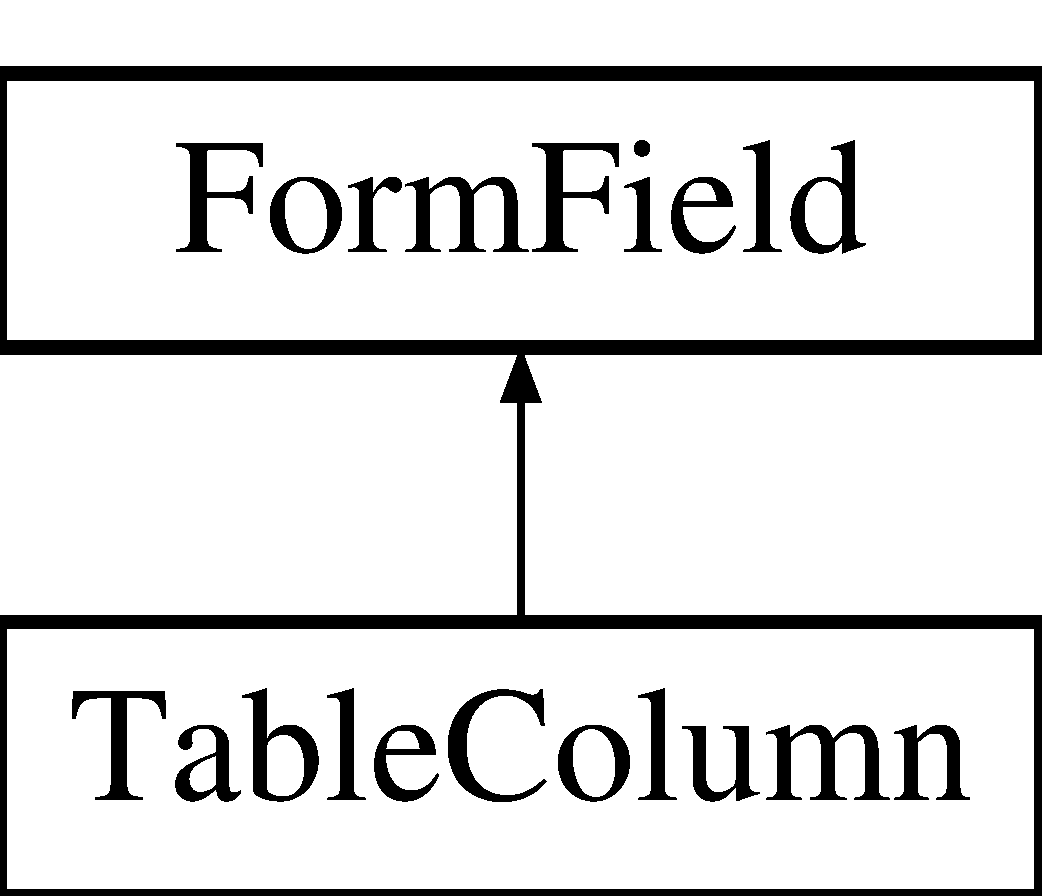
\includegraphics[height=2.000000cm]{classFormField}
\end{center}
\end{figure}
\subsection*{Public Member Functions}
\begin{DoxyCompactItemize}
\item 
\hyperlink{classFormField_a7208af5aa5a791c9c86148d6cb66b9f8}{FormField} (QObject $\ast$parent=0)
\item 
QString \hyperlink{classFormField_a215caa284c220e889de7fa96bba4adf5}{name} ()
\item 
void \hyperlink{classFormField_a377c8c0b78a87bae4aa18be92f00e48a}{setName} (QString)
\item 
QString \hyperlink{classFormField_a7039517b94a2320fca6c834a412fb6b9}{colName} ()
\item 
void \hyperlink{classFormField_a359314a81978dc6dd169f84ec91de066}{setColName} (QString)
\item 
QString \hyperlink{classFormField_a28963efac4457b6d7312e9a1cb2e487c}{sqlTabName} ()
\item 
void \hyperlink{classFormField_a6d1dc5a4a95ef91a78b3bb271d581a59}{setSqlTabName} (QString)
\item 
QString \hyperlink{classFormField_a04114033387a664667d67b14defb0850}{sqlType} ()
\item 
void \hyperlink{classFormField_a7f4a7c832ff7670d69288b2a1e370e35}{setSqlType} (QString)
\item 
bool \hyperlink{classFormField_a4790898b5c806db22925ec6322191b89}{noEntry} ()
\item 
void \hyperlink{classFormField_a96b15a7a89e7d7e8fabae2cc40d6c5bb}{setNoEntry} (bool)
\item 
bool \hyperlink{classFormField_a0f409108a33cae8d0e22082f5f26f6a2}{notNull} ()
\item 
void \hyperlink{classFormField_ad36a82ba7392e37477cdc1b4ffe3e62a}{setNotNull} (bool)
\item 
bool \hyperlink{classFormField_a367a5f4ac96d07a32a0e1a6c21e89a11}{hidden} ()
\item 
void \hyperlink{classFormField_a3d20d4327791a7841305add68e458555}{setHidden} (bool)
\item 
bool \hyperlink{classFormField_aafaf8e53177986629c92bb019b4416bd}{required} ()
\item 
void \hyperlink{classFormField_a77ecd265c65bb495e52312806f15becc}{setRequired} (bool)
\item 
int \hyperlink{classFormField_a482265a6cc61b55254c32ab3bfe896ed}{fieldId} ()
\item 
void \hyperlink{classFormField_a6da3ec71e2e22b2eca8151c08663f0d2}{setFieldId} (int)
\item 
int \hyperlink{classFormField_a9296ae3d1322bce37f7606cd4ba063ce}{tabIndex} ()
\item 
void \hyperlink{classFormField_a860545288d309640181ff72a031073e0}{setTabIndex} (int)
\item 
bool \hyperlink{classFormField_ae1d2052bc5a3ac7a387ada02c9468cfe}{touched} ()
\item 
void \hyperlink{classFormField_a9888cc6ba39d58222ca63f15a439c038}{setFormat} (QString f)
\item 
QString \hyperlink{classFormField_aa46924cdfef9aff52746c5e288c3fe39}{format} ()
\item 
QString \hyperlink{classFormField_acf9200a7add35df526f73b3b6979196f}{defaultValue} ()
\item 
void \hyperlink{classFormField_a847edff4ea53c51206b7647156ac35e0}{setDefaultValue} (QString)
\item 
void \hyperlink{classFormField_a9e7ab4c532d7445e3bb17ce91b4edd2f}{addField} (QWidget $\ast$)
\item 
QDomDocument \hyperlink{classFormField_a687303cd0e40108fa62becf42ae36afa}{toXML} ()
\end{DoxyCompactItemize}
\subsection*{Protected Member Functions}
\begin{DoxyCompactItemize}
\item 
void \hyperlink{classFormField_a95d519466092fca7255ef0fe02551b99}{setTouched} (bool)
\end{DoxyCompactItemize}
\subsection*{Protected Attributes}
\begin{DoxyCompactItemize}
\item 
QString \hyperlink{classFormField_a7678a3e5f30d707b47b4b1a23a9bd80d}{qs\_\-name}
\item 
QString \hyperlink{classFormField_ac8f496b75a15cf55a93c5bbd0cd3c037}{qs\_\-format}
\item 
QString \hyperlink{classFormField_ad05d2212596727bd118e8b2c1f57f7b7}{qs\_\-colName}
\item 
QString \hyperlink{classFormField_a525f52fa7e6e96ee123d77eb1e81ab1f}{qs\_\-sqlTabName}
\item 
QString \hyperlink{classFormField_a64e90014c3119fd3981be4fcceacf361}{qs\_\-sqlType}
\item 
QString \hyperlink{classFormField_aa2bdc2d8032046b7ed7645c8a8e21ba2}{qs\_\-defaultValue}
\item 
bool \hyperlink{classFormField_a4623e1801da0e00ab26dc269a6d20caf}{b\_\-noEntry}
\item 
bool \hyperlink{classFormField_ad65ad13b03617a86b52ea49312aa9dac}{b\_\-notNull}
\item 
bool \hyperlink{classFormField_ad99a28a6bd3a93e1e3917d95f29d3ed7}{b\_\-required}
\item 
bool \hyperlink{classFormField_ab9d3090ff6e5c9f324c693c6fc583268}{b\_\-hidden}
\item 
int \hyperlink{classFormField_a19f3e77df8c8caf716c3539f49405d96}{i\_\-fieldId}
\item 
int \hyperlink{classFormField_ac4fd32b1bbf15117330290e4116e552a}{i\_\-tabIndex}
\item 
bool \hyperlink{classFormField_a09105b3e8fc915c9f2bf327fa2723723}{b\_\-touched}
\item 
QWidget $\ast$ \hyperlink{classFormField_ab7f3ad82c182c8a4989713f3f1816184}{p\_\-field}
\end{DoxyCompactItemize}
\subsection*{Private Attributes}
\begin{DoxyCompactItemize}
\item 
QString \hyperlink{classFormField_a1263d00231a1badf214a51c4062f9118}{qs\_\-text}
\end{DoxyCompactItemize}


\subsection{Detailed Description}


Definition at line 45 of file vwidgets.h.



\subsection{Constructor \& Destructor Documentation}
\hypertarget{classFormField_a7208af5aa5a791c9c86148d6cb66b9f8}{
\index{FormField@{FormField}!FormField@{FormField}}
\index{FormField@{FormField}!FormField@{FormField}}
\subsubsection[{FormField}]{\setlength{\rightskip}{0pt plus 5cm}FormField::FormField (
\begin{DoxyParamCaption}
\item[{QObject $\ast$}]{parent = {\ttfamily 0}}
\end{DoxyParamCaption}
)}}
\label{classFormField_a7208af5aa5a791c9c86148d6cb66b9f8}


Definition at line 38 of file vwidgets.cpp.



\subsection{Member Function Documentation}
\hypertarget{classFormField_a9e7ab4c532d7445e3bb17ce91b4edd2f}{
\index{FormField@{FormField}!addField@{addField}}
\index{addField@{addField}!FormField@{FormField}}
\subsubsection[{addField}]{\setlength{\rightskip}{0pt plus 5cm}void FormField::addField (
\begin{DoxyParamCaption}
\item[{QWidget $\ast$}]{widget}
\end{DoxyParamCaption}
)}}
\label{classFormField_a9e7ab4c532d7445e3bb17ce91b4edd2f}


Definition at line 205 of file vwidgets.cpp.

\hypertarget{classFormField_a7039517b94a2320fca6c834a412fb6b9}{
\index{FormField@{FormField}!colName@{colName}}
\index{colName@{colName}!FormField@{FormField}}
\subsubsection[{colName}]{\setlength{\rightskip}{0pt plus 5cm}QString FormField::colName (
\begin{DoxyParamCaption}
{}
\end{DoxyParamCaption}
)}}
\label{classFormField_a7039517b94a2320fca6c834a412fb6b9}


Definition at line 65 of file vwidgets.cpp.

\hypertarget{classFormField_acf9200a7add35df526f73b3b6979196f}{
\index{FormField@{FormField}!defaultValue@{defaultValue}}
\index{defaultValue@{defaultValue}!FormField@{FormField}}
\subsubsection[{defaultValue}]{\setlength{\rightskip}{0pt plus 5cm}QString FormField::defaultValue (
\begin{DoxyParamCaption}
{}
\end{DoxyParamCaption}
)}}
\label{classFormField_acf9200a7add35df526f73b3b6979196f}


Definition at line 193 of file vwidgets.cpp.

\hypertarget{classFormField_a482265a6cc61b55254c32ab3bfe896ed}{
\index{FormField@{FormField}!fieldId@{fieldId}}
\index{fieldId@{fieldId}!FormField@{FormField}}
\subsubsection[{fieldId}]{\setlength{\rightskip}{0pt plus 5cm}int FormField::fieldId (
\begin{DoxyParamCaption}
{}
\end{DoxyParamCaption}
)}}
\label{classFormField_a482265a6cc61b55254c32ab3bfe896ed}


Definition at line 149 of file vwidgets.cpp.

\hypertarget{classFormField_aa46924cdfef9aff52746c5e288c3fe39}{
\index{FormField@{FormField}!format@{format}}
\index{format@{format}!FormField@{FormField}}
\subsubsection[{format}]{\setlength{\rightskip}{0pt plus 5cm}QString FormField::format (
\begin{DoxyParamCaption}
{}
\end{DoxyParamCaption}
)\hspace{0.3cm}{\ttfamily  \mbox{[}inline\mbox{]}}}}
\label{classFormField_aa46924cdfef9aff52746c5e288c3fe39}


Definition at line 73 of file vwidgets.h.

\hypertarget{classFormField_a367a5f4ac96d07a32a0e1a6c21e89a11}{
\index{FormField@{FormField}!hidden@{hidden}}
\index{hidden@{hidden}!FormField@{FormField}}
\subsubsection[{hidden}]{\setlength{\rightskip}{0pt plus 5cm}bool FormField::hidden (
\begin{DoxyParamCaption}
{}
\end{DoxyParamCaption}
)}}
\label{classFormField_a367a5f4ac96d07a32a0e1a6c21e89a11}


Definition at line 125 of file vwidgets.cpp.

\hypertarget{classFormField_a215caa284c220e889de7fa96bba4adf5}{
\index{FormField@{FormField}!name@{name}}
\index{name@{name}!FormField@{FormField}}
\subsubsection[{name}]{\setlength{\rightskip}{0pt plus 5cm}QString FormField::name (
\begin{DoxyParamCaption}
{}
\end{DoxyParamCaption}
)}}
\label{classFormField_a215caa284c220e889de7fa96bba4adf5}


Definition at line 53 of file vwidgets.cpp.

\hypertarget{classFormField_a4790898b5c806db22925ec6322191b89}{
\index{FormField@{FormField}!noEntry@{noEntry}}
\index{noEntry@{noEntry}!FormField@{FormField}}
\subsubsection[{noEntry}]{\setlength{\rightskip}{0pt plus 5cm}bool FormField::noEntry (
\begin{DoxyParamCaption}
{}
\end{DoxyParamCaption}
)}}
\label{classFormField_a4790898b5c806db22925ec6322191b89}


Definition at line 101 of file vwidgets.cpp.

\hypertarget{classFormField_a0f409108a33cae8d0e22082f5f26f6a2}{
\index{FormField@{FormField}!notNull@{notNull}}
\index{notNull@{notNull}!FormField@{FormField}}
\subsubsection[{notNull}]{\setlength{\rightskip}{0pt plus 5cm}bool FormField::notNull (
\begin{DoxyParamCaption}
{}
\end{DoxyParamCaption}
)}}
\label{classFormField_a0f409108a33cae8d0e22082f5f26f6a2}


Definition at line 113 of file vwidgets.cpp.

\hypertarget{classFormField_aafaf8e53177986629c92bb019b4416bd}{
\index{FormField@{FormField}!required@{required}}
\index{required@{required}!FormField@{FormField}}
\subsubsection[{required}]{\setlength{\rightskip}{0pt plus 5cm}bool FormField::required (
\begin{DoxyParamCaption}
{}
\end{DoxyParamCaption}
)}}
\label{classFormField_aafaf8e53177986629c92bb019b4416bd}


Definition at line 137 of file vwidgets.cpp.

\hypertarget{classFormField_a359314a81978dc6dd169f84ec91de066}{
\index{FormField@{FormField}!setColName@{setColName}}
\index{setColName@{setColName}!FormField@{FormField}}
\subsubsection[{setColName}]{\setlength{\rightskip}{0pt plus 5cm}void FormField::setColName (
\begin{DoxyParamCaption}
\item[{QString}]{colName}
\end{DoxyParamCaption}
)}}
\label{classFormField_a359314a81978dc6dd169f84ec91de066}


Definition at line 71 of file vwidgets.cpp.

\hypertarget{classFormField_a847edff4ea53c51206b7647156ac35e0}{
\index{FormField@{FormField}!setDefaultValue@{setDefaultValue}}
\index{setDefaultValue@{setDefaultValue}!FormField@{FormField}}
\subsubsection[{setDefaultValue}]{\setlength{\rightskip}{0pt plus 5cm}void FormField::setDefaultValue (
\begin{DoxyParamCaption}
\item[{QString}]{val}
\end{DoxyParamCaption}
)}}
\label{classFormField_a847edff4ea53c51206b7647156ac35e0}


Definition at line 199 of file vwidgets.cpp.

\hypertarget{classFormField_a6da3ec71e2e22b2eca8151c08663f0d2}{
\index{FormField@{FormField}!setFieldId@{setFieldId}}
\index{setFieldId@{setFieldId}!FormField@{FormField}}
\subsubsection[{setFieldId}]{\setlength{\rightskip}{0pt plus 5cm}void FormField::setFieldId (
\begin{DoxyParamCaption}
\item[{int}]{id}
\end{DoxyParamCaption}
)}}
\label{classFormField_a6da3ec71e2e22b2eca8151c08663f0d2}


Definition at line 155 of file vwidgets.cpp.

\hypertarget{classFormField_a9888cc6ba39d58222ca63f15a439c038}{
\index{FormField@{FormField}!setFormat@{setFormat}}
\index{setFormat@{setFormat}!FormField@{FormField}}
\subsubsection[{setFormat}]{\setlength{\rightskip}{0pt plus 5cm}void FormField::setFormat (
\begin{DoxyParamCaption}
\item[{QString}]{f}
\end{DoxyParamCaption}
)\hspace{0.3cm}{\ttfamily  \mbox{[}inline\mbox{]}}}}
\label{classFormField_a9888cc6ba39d58222ca63f15a439c038}


Definition at line 72 of file vwidgets.h.

\hypertarget{classFormField_a3d20d4327791a7841305add68e458555}{
\index{FormField@{FormField}!setHidden@{setHidden}}
\index{setHidden@{setHidden}!FormField@{FormField}}
\subsubsection[{setHidden}]{\setlength{\rightskip}{0pt plus 5cm}void FormField::setHidden (
\begin{DoxyParamCaption}
\item[{bool}]{hidden}
\end{DoxyParamCaption}
)}}
\label{classFormField_a3d20d4327791a7841305add68e458555}


Definition at line 131 of file vwidgets.cpp.

\hypertarget{classFormField_a377c8c0b78a87bae4aa18be92f00e48a}{
\index{FormField@{FormField}!setName@{setName}}
\index{setName@{setName}!FormField@{FormField}}
\subsubsection[{setName}]{\setlength{\rightskip}{0pt plus 5cm}void FormField::setName (
\begin{DoxyParamCaption}
\item[{QString}]{name}
\end{DoxyParamCaption}
)}}
\label{classFormField_a377c8c0b78a87bae4aa18be92f00e48a}


Definition at line 59 of file vwidgets.cpp.

\hypertarget{classFormField_a96b15a7a89e7d7e8fabae2cc40d6c5bb}{
\index{FormField@{FormField}!setNoEntry@{setNoEntry}}
\index{setNoEntry@{setNoEntry}!FormField@{FormField}}
\subsubsection[{setNoEntry}]{\setlength{\rightskip}{0pt plus 5cm}void FormField::setNoEntry (
\begin{DoxyParamCaption}
\item[{bool}]{noEntry}
\end{DoxyParamCaption}
)}}
\label{classFormField_a96b15a7a89e7d7e8fabae2cc40d6c5bb}


Definition at line 107 of file vwidgets.cpp.

\hypertarget{classFormField_ad36a82ba7392e37477cdc1b4ffe3e62a}{
\index{FormField@{FormField}!setNotNull@{setNotNull}}
\index{setNotNull@{setNotNull}!FormField@{FormField}}
\subsubsection[{setNotNull}]{\setlength{\rightskip}{0pt plus 5cm}void FormField::setNotNull (
\begin{DoxyParamCaption}
\item[{bool}]{notNull}
\end{DoxyParamCaption}
)}}
\label{classFormField_ad36a82ba7392e37477cdc1b4ffe3e62a}


Definition at line 119 of file vwidgets.cpp.

\hypertarget{classFormField_a77ecd265c65bb495e52312806f15becc}{
\index{FormField@{FormField}!setRequired@{setRequired}}
\index{setRequired@{setRequired}!FormField@{FormField}}
\subsubsection[{setRequired}]{\setlength{\rightskip}{0pt plus 5cm}void FormField::setRequired (
\begin{DoxyParamCaption}
\item[{bool}]{req}
\end{DoxyParamCaption}
)}}
\label{classFormField_a77ecd265c65bb495e52312806f15becc}


Definition at line 143 of file vwidgets.cpp.

\hypertarget{classFormField_a6d1dc5a4a95ef91a78b3bb271d581a59}{
\index{FormField@{FormField}!setSqlTabName@{setSqlTabName}}
\index{setSqlTabName@{setSqlTabName}!FormField@{FormField}}
\subsubsection[{setSqlTabName}]{\setlength{\rightskip}{0pt plus 5cm}void FormField::setSqlTabName (
\begin{DoxyParamCaption}
\item[{QString}]{tabName}
\end{DoxyParamCaption}
)}}
\label{classFormField_a6d1dc5a4a95ef91a78b3bb271d581a59}


Definition at line 83 of file vwidgets.cpp.

\hypertarget{classFormField_a7f4a7c832ff7670d69288b2a1e370e35}{
\index{FormField@{FormField}!setSqlType@{setSqlType}}
\index{setSqlType@{setSqlType}!FormField@{FormField}}
\subsubsection[{setSqlType}]{\setlength{\rightskip}{0pt plus 5cm}void FormField::setSqlType (
\begin{DoxyParamCaption}
\item[{QString}]{sqlType}
\end{DoxyParamCaption}
)}}
\label{classFormField_a7f4a7c832ff7670d69288b2a1e370e35}


Definition at line 95 of file vwidgets.cpp.

\hypertarget{classFormField_a860545288d309640181ff72a031073e0}{
\index{FormField@{FormField}!setTabIndex@{setTabIndex}}
\index{setTabIndex@{setTabIndex}!FormField@{FormField}}
\subsubsection[{setTabIndex}]{\setlength{\rightskip}{0pt plus 5cm}void FormField::setTabIndex (
\begin{DoxyParamCaption}
\item[{int}]{ti}
\end{DoxyParamCaption}
)}}
\label{classFormField_a860545288d309640181ff72a031073e0}


Definition at line 167 of file vwidgets.cpp.

\hypertarget{classFormField_a95d519466092fca7255ef0fe02551b99}{
\index{FormField@{FormField}!setTouched@{setTouched}}
\index{setTouched@{setTouched}!FormField@{FormField}}
\subsubsection[{setTouched}]{\setlength{\rightskip}{0pt plus 5cm}void FormField::setTouched (
\begin{DoxyParamCaption}
\item[{bool}]{}
\end{DoxyParamCaption}
)\hspace{0.3cm}{\ttfamily  \mbox{[}protected\mbox{]}}}}
\label{classFormField_a95d519466092fca7255ef0fe02551b99}
\hypertarget{classFormField_a28963efac4457b6d7312e9a1cb2e487c}{
\index{FormField@{FormField}!sqlTabName@{sqlTabName}}
\index{sqlTabName@{sqlTabName}!FormField@{FormField}}
\subsubsection[{sqlTabName}]{\setlength{\rightskip}{0pt plus 5cm}QString FormField::sqlTabName (
\begin{DoxyParamCaption}
{}
\end{DoxyParamCaption}
)}}
\label{classFormField_a28963efac4457b6d7312e9a1cb2e487c}


Definition at line 77 of file vwidgets.cpp.

\hypertarget{classFormField_a04114033387a664667d67b14defb0850}{
\index{FormField@{FormField}!sqlType@{sqlType}}
\index{sqlType@{sqlType}!FormField@{FormField}}
\subsubsection[{sqlType}]{\setlength{\rightskip}{0pt plus 5cm}QString FormField::sqlType (
\begin{DoxyParamCaption}
{}
\end{DoxyParamCaption}
)}}
\label{classFormField_a04114033387a664667d67b14defb0850}


Definition at line 89 of file vwidgets.cpp.

\hypertarget{classFormField_a9296ae3d1322bce37f7606cd4ba063ce}{
\index{FormField@{FormField}!tabIndex@{tabIndex}}
\index{tabIndex@{tabIndex}!FormField@{FormField}}
\subsubsection[{tabIndex}]{\setlength{\rightskip}{0pt plus 5cm}int FormField::tabIndex (
\begin{DoxyParamCaption}
{}
\end{DoxyParamCaption}
)}}
\label{classFormField_a9296ae3d1322bce37f7606cd4ba063ce}


Definition at line 161 of file vwidgets.cpp.

\hypertarget{classFormField_ae1d2052bc5a3ac7a387ada02c9468cfe}{
\index{FormField@{FormField}!touched@{touched}}
\index{touched@{touched}!FormField@{FormField}}
\subsubsection[{touched}]{\setlength{\rightskip}{0pt plus 5cm}bool FormField::touched (
\begin{DoxyParamCaption}
{}
\end{DoxyParamCaption}
)}}
\label{classFormField_ae1d2052bc5a3ac7a387ada02c9468cfe}


Definition at line 173 of file vwidgets.cpp.

\hypertarget{classFormField_a687303cd0e40108fa62becf42ae36afa}{
\index{FormField@{FormField}!toXML@{toXML}}
\index{toXML@{toXML}!FormField@{FormField}}
\subsubsection[{toXML}]{\setlength{\rightskip}{0pt plus 5cm}QDomDocument FormField::toXML (
\begin{DoxyParamCaption}
{}
\end{DoxyParamCaption}
)}}
\label{classFormField_a687303cd0e40108fa62becf42ae36afa}


Definition at line 212 of file vwidgets.cpp.



\subsection{Member Data Documentation}
\hypertarget{classFormField_ab9d3090ff6e5c9f324c693c6fc583268}{
\index{FormField@{FormField}!b\_\-hidden@{b\_\-hidden}}
\index{b\_\-hidden@{b\_\-hidden}!FormField@{FormField}}
\subsubsection[{b\_\-hidden}]{\setlength{\rightskip}{0pt plus 5cm}bool {\bf FormField::b\_\-hidden}\hspace{0.3cm}{\ttfamily  \mbox{[}protected\mbox{]}}}}
\label{classFormField_ab9d3090ff6e5c9f324c693c6fc583268}


Definition at line 96 of file vwidgets.h.

\hypertarget{classFormField_a4623e1801da0e00ab26dc269a6d20caf}{
\index{FormField@{FormField}!b\_\-noEntry@{b\_\-noEntry}}
\index{b\_\-noEntry@{b\_\-noEntry}!FormField@{FormField}}
\subsubsection[{b\_\-noEntry}]{\setlength{\rightskip}{0pt plus 5cm}bool {\bf FormField::b\_\-noEntry}\hspace{0.3cm}{\ttfamily  \mbox{[}protected\mbox{]}}}}
\label{classFormField_a4623e1801da0e00ab26dc269a6d20caf}


Definition at line 93 of file vwidgets.h.

\hypertarget{classFormField_ad65ad13b03617a86b52ea49312aa9dac}{
\index{FormField@{FormField}!b\_\-notNull@{b\_\-notNull}}
\index{b\_\-notNull@{b\_\-notNull}!FormField@{FormField}}
\subsubsection[{b\_\-notNull}]{\setlength{\rightskip}{0pt plus 5cm}bool {\bf FormField::b\_\-notNull}\hspace{0.3cm}{\ttfamily  \mbox{[}protected\mbox{]}}}}
\label{classFormField_ad65ad13b03617a86b52ea49312aa9dac}


Definition at line 94 of file vwidgets.h.

\hypertarget{classFormField_ad99a28a6bd3a93e1e3917d95f29d3ed7}{
\index{FormField@{FormField}!b\_\-required@{b\_\-required}}
\index{b\_\-required@{b\_\-required}!FormField@{FormField}}
\subsubsection[{b\_\-required}]{\setlength{\rightskip}{0pt plus 5cm}bool {\bf FormField::b\_\-required}\hspace{0.3cm}{\ttfamily  \mbox{[}protected\mbox{]}}}}
\label{classFormField_ad99a28a6bd3a93e1e3917d95f29d3ed7}


Definition at line 95 of file vwidgets.h.

\hypertarget{classFormField_a09105b3e8fc915c9f2bf327fa2723723}{
\index{FormField@{FormField}!b\_\-touched@{b\_\-touched}}
\index{b\_\-touched@{b\_\-touched}!FormField@{FormField}}
\subsubsection[{b\_\-touched}]{\setlength{\rightskip}{0pt plus 5cm}bool {\bf FormField::b\_\-touched}\hspace{0.3cm}{\ttfamily  \mbox{[}protected\mbox{]}}}}
\label{classFormField_a09105b3e8fc915c9f2bf327fa2723723}


Definition at line 99 of file vwidgets.h.

\hypertarget{classFormField_a19f3e77df8c8caf716c3539f49405d96}{
\index{FormField@{FormField}!i\_\-fieldId@{i\_\-fieldId}}
\index{i\_\-fieldId@{i\_\-fieldId}!FormField@{FormField}}
\subsubsection[{i\_\-fieldId}]{\setlength{\rightskip}{0pt plus 5cm}int {\bf FormField::i\_\-fieldId}\hspace{0.3cm}{\ttfamily  \mbox{[}protected\mbox{]}}}}
\label{classFormField_a19f3e77df8c8caf716c3539f49405d96}


Definition at line 97 of file vwidgets.h.

\hypertarget{classFormField_ac4fd32b1bbf15117330290e4116e552a}{
\index{FormField@{FormField}!i\_\-tabIndex@{i\_\-tabIndex}}
\index{i\_\-tabIndex@{i\_\-tabIndex}!FormField@{FormField}}
\subsubsection[{i\_\-tabIndex}]{\setlength{\rightskip}{0pt plus 5cm}int {\bf FormField::i\_\-tabIndex}\hspace{0.3cm}{\ttfamily  \mbox{[}protected\mbox{]}}}}
\label{classFormField_ac4fd32b1bbf15117330290e4116e552a}


Definition at line 98 of file vwidgets.h.

\hypertarget{classFormField_ab7f3ad82c182c8a4989713f3f1816184}{
\index{FormField@{FormField}!p\_\-field@{p\_\-field}}
\index{p\_\-field@{p\_\-field}!FormField@{FormField}}
\subsubsection[{p\_\-field}]{\setlength{\rightskip}{0pt plus 5cm}QWidget$\ast$ {\bf FormField::p\_\-field}\hspace{0.3cm}{\ttfamily  \mbox{[}protected\mbox{]}}}}
\label{classFormField_ab7f3ad82c182c8a4989713f3f1816184}


Definition at line 101 of file vwidgets.h.

\hypertarget{classFormField_ad05d2212596727bd118e8b2c1f57f7b7}{
\index{FormField@{FormField}!qs\_\-colName@{qs\_\-colName}}
\index{qs\_\-colName@{qs\_\-colName}!FormField@{FormField}}
\subsubsection[{qs\_\-colName}]{\setlength{\rightskip}{0pt plus 5cm}QString {\bf FormField::qs\_\-colName}\hspace{0.3cm}{\ttfamily  \mbox{[}protected\mbox{]}}}}
\label{classFormField_ad05d2212596727bd118e8b2c1f57f7b7}


Definition at line 89 of file vwidgets.h.

\hypertarget{classFormField_aa2bdc2d8032046b7ed7645c8a8e21ba2}{
\index{FormField@{FormField}!qs\_\-defaultValue@{qs\_\-defaultValue}}
\index{qs\_\-defaultValue@{qs\_\-defaultValue}!FormField@{FormField}}
\subsubsection[{qs\_\-defaultValue}]{\setlength{\rightskip}{0pt plus 5cm}QString {\bf FormField::qs\_\-defaultValue}\hspace{0.3cm}{\ttfamily  \mbox{[}protected\mbox{]}}}}
\label{classFormField_aa2bdc2d8032046b7ed7645c8a8e21ba2}


Definition at line 92 of file vwidgets.h.

\hypertarget{classFormField_ac8f496b75a15cf55a93c5bbd0cd3c037}{
\index{FormField@{FormField}!qs\_\-format@{qs\_\-format}}
\index{qs\_\-format@{qs\_\-format}!FormField@{FormField}}
\subsubsection[{qs\_\-format}]{\setlength{\rightskip}{0pt plus 5cm}QString {\bf FormField::qs\_\-format}\hspace{0.3cm}{\ttfamily  \mbox{[}protected\mbox{]}}}}
\label{classFormField_ac8f496b75a15cf55a93c5bbd0cd3c037}


Definition at line 88 of file vwidgets.h.

\hypertarget{classFormField_a7678a3e5f30d707b47b4b1a23a9bd80d}{
\index{FormField@{FormField}!qs\_\-name@{qs\_\-name}}
\index{qs\_\-name@{qs\_\-name}!FormField@{FormField}}
\subsubsection[{qs\_\-name}]{\setlength{\rightskip}{0pt plus 5cm}QString {\bf FormField::qs\_\-name}\hspace{0.3cm}{\ttfamily  \mbox{[}protected\mbox{]}}}}
\label{classFormField_a7678a3e5f30d707b47b4b1a23a9bd80d}


Definition at line 87 of file vwidgets.h.

\hypertarget{classFormField_a525f52fa7e6e96ee123d77eb1e81ab1f}{
\index{FormField@{FormField}!qs\_\-sqlTabName@{qs\_\-sqlTabName}}
\index{qs\_\-sqlTabName@{qs\_\-sqlTabName}!FormField@{FormField}}
\subsubsection[{qs\_\-sqlTabName}]{\setlength{\rightskip}{0pt plus 5cm}QString {\bf FormField::qs\_\-sqlTabName}\hspace{0.3cm}{\ttfamily  \mbox{[}protected\mbox{]}}}}
\label{classFormField_a525f52fa7e6e96ee123d77eb1e81ab1f}


Definition at line 90 of file vwidgets.h.

\hypertarget{classFormField_a64e90014c3119fd3981be4fcceacf361}{
\index{FormField@{FormField}!qs\_\-sqlType@{qs\_\-sqlType}}
\index{qs\_\-sqlType@{qs\_\-sqlType}!FormField@{FormField}}
\subsubsection[{qs\_\-sqlType}]{\setlength{\rightskip}{0pt plus 5cm}QString {\bf FormField::qs\_\-sqlType}\hspace{0.3cm}{\ttfamily  \mbox{[}protected\mbox{]}}}}
\label{classFormField_a64e90014c3119fd3981be4fcceacf361}


Definition at line 91 of file vwidgets.h.

\hypertarget{classFormField_a1263d00231a1badf214a51c4062f9118}{
\index{FormField@{FormField}!qs\_\-text@{qs\_\-text}}
\index{qs\_\-text@{qs\_\-text}!FormField@{FormField}}
\subsubsection[{qs\_\-text}]{\setlength{\rightskip}{0pt plus 5cm}QString {\bf FormField::qs\_\-text}\hspace{0.3cm}{\ttfamily  \mbox{[}private\mbox{]}}}}
\label{classFormField_a1263d00231a1badf214a51c4062f9118}


Definition at line 84 of file vwidgets.h.



The documentation for this class was generated from the following files:\begin{DoxyCompactItemize}
\item 
/e/ms/QT/models/\hyperlink{vwidgets_8h}{vwidgets.h}\item 
/e/ms/QT/models/\hyperlink{vwidgets_8cpp}{vwidgets.cpp}\end{DoxyCompactItemize}

\hypertarget{classLabel}{
\section{Label Class Reference}
\label{classLabel}\index{Label@{Label}}
}


{\ttfamily \#include $<$vwidgets.h$>$}

\subsection*{Public Member Functions}
\begin{DoxyCompactItemize}
\item 
\hyperlink{classLabel_a8f43a231b00daa09d72a7263dca2b107}{Label} (QWidget $\ast$parent=0)
\item 
\hyperlink{classLabel_a24fbd6634f58ecd6c2f6db26dea484db}{Label} (const QString \&text, QWidget $\ast$parent=0)
\end{DoxyCompactItemize}
\subsection*{Public Attributes}
\begin{DoxyCompactItemize}
\item 
QString \hyperlink{classLabel_a5584bf11b1059f5c48ee4ed0e074e5b3}{sqlTabName}
\item 
QString \hyperlink{classLabel_a9456abb423939d68c1671b796abf92d8}{name}
\item 
QString \hyperlink{classLabel_a484912d15ccb6b509a438ded54ec4db8}{colName}
\item 
bool \hyperlink{classLabel_a41e67ddc798145020945bf373032788d}{img}
\item 
int \hyperlink{classLabel_a8339b81ceaa1dab691f57cea88886e86}{x}
\item 
int \hyperlink{classLabel_af7de5d7b7af764667a51747ba6fd5a2e}{y}
\item 
int \hyperlink{classLabel_ac1b8873ac4b399c5f70305b08aa7f5c8}{w}
\end{DoxyCompactItemize}


\subsection{Detailed Description}


Definition at line 312 of file vwidgets.h.



\subsection{Constructor \& Destructor Documentation}
\hypertarget{classLabel_a8f43a231b00daa09d72a7263dca2b107}{
\index{Label@{Label}!Label@{Label}}
\index{Label@{Label}!Label@{Label}}
\subsubsection[{Label}]{\setlength{\rightskip}{0pt plus 5cm}Label::Label (
\begin{DoxyParamCaption}
\item[{QWidget $\ast$}]{parent = {\ttfamily 0}}
\end{DoxyParamCaption}
)}}
\label{classLabel_a8f43a231b00daa09d72a7263dca2b107}


Definition at line 2344 of file vwidgets.cpp.

\hypertarget{classLabel_a24fbd6634f58ecd6c2f6db26dea484db}{
\index{Label@{Label}!Label@{Label}}
\index{Label@{Label}!Label@{Label}}
\subsubsection[{Label}]{\setlength{\rightskip}{0pt plus 5cm}Label::Label (
\begin{DoxyParamCaption}
\item[{const QString \&}]{text, }
\item[{QWidget $\ast$}]{parent = {\ttfamily 0}}
\end{DoxyParamCaption}
)}}
\label{classLabel_a24fbd6634f58ecd6c2f6db26dea484db}


Definition at line 2302 of file vwidgets.cpp.



\subsection{Member Data Documentation}
\hypertarget{classLabel_a484912d15ccb6b509a438ded54ec4db8}{
\index{Label@{Label}!colName@{colName}}
\index{colName@{colName}!Label@{Label}}
\subsubsection[{colName}]{\setlength{\rightskip}{0pt plus 5cm}QString {\bf Label::colName}}}
\label{classLabel_a484912d15ccb6b509a438ded54ec4db8}


Definition at line 321 of file vwidgets.h.

\hypertarget{classLabel_a41e67ddc798145020945bf373032788d}{
\index{Label@{Label}!img@{img}}
\index{img@{img}!Label@{Label}}
\subsubsection[{img}]{\setlength{\rightskip}{0pt plus 5cm}bool {\bf Label::img}}}
\label{classLabel_a41e67ddc798145020945bf373032788d}


Definition at line 322 of file vwidgets.h.

\hypertarget{classLabel_a9456abb423939d68c1671b796abf92d8}{
\index{Label@{Label}!name@{name}}
\index{name@{name}!Label@{Label}}
\subsubsection[{name}]{\setlength{\rightskip}{0pt plus 5cm}QString {\bf Label::name}}}
\label{classLabel_a9456abb423939d68c1671b796abf92d8}


Definition at line 320 of file vwidgets.h.

\hypertarget{classLabel_a5584bf11b1059f5c48ee4ed0e074e5b3}{
\index{Label@{Label}!sqlTabName@{sqlTabName}}
\index{sqlTabName@{sqlTabName}!Label@{Label}}
\subsubsection[{sqlTabName}]{\setlength{\rightskip}{0pt plus 5cm}QString {\bf Label::sqlTabName}}}
\label{classLabel_a5584bf11b1059f5c48ee4ed0e074e5b3}


Definition at line 319 of file vwidgets.h.

\hypertarget{classLabel_ac1b8873ac4b399c5f70305b08aa7f5c8}{
\index{Label@{Label}!w@{w}}
\index{w@{w}!Label@{Label}}
\subsubsection[{w}]{\setlength{\rightskip}{0pt plus 5cm}int {\bf Label::w}}}
\label{classLabel_ac1b8873ac4b399c5f70305b08aa7f5c8}


Definition at line 324 of file vwidgets.h.

\hypertarget{classLabel_a8339b81ceaa1dab691f57cea88886e86}{
\index{Label@{Label}!x@{x}}
\index{x@{x}!Label@{Label}}
\subsubsection[{x}]{\setlength{\rightskip}{0pt plus 5cm}int {\bf Label::x}}}
\label{classLabel_a8339b81ceaa1dab691f57cea88886e86}


Definition at line 324 of file vwidgets.h.

\hypertarget{classLabel_af7de5d7b7af764667a51747ba6fd5a2e}{
\index{Label@{Label}!y@{y}}
\index{y@{y}!Label@{Label}}
\subsubsection[{y}]{\setlength{\rightskip}{0pt plus 5cm}int {\bf Label::y}}}
\label{classLabel_af7de5d7b7af764667a51747ba6fd5a2e}


Definition at line 324 of file vwidgets.h.



The documentation for this class was generated from the following files:\begin{DoxyCompactItemize}
\item 
/e/ms/QT/models/\hyperlink{vwidgets_8h}{vwidgets.h}\item 
/e/ms/QT/models/\hyperlink{vwidgets_8cpp}{vwidgets.cpp}\end{DoxyCompactItemize}

\hypertarget{classLineEdit}{
\section{LineEdit Class Reference}
\label{classLineEdit}\index{LineEdit@{LineEdit}}
}


{\ttfamily \#include $<$vwidgets.h$>$}

Inheritance diagram for LineEdit:\begin{figure}[H]
\begin{center}
\leavevmode
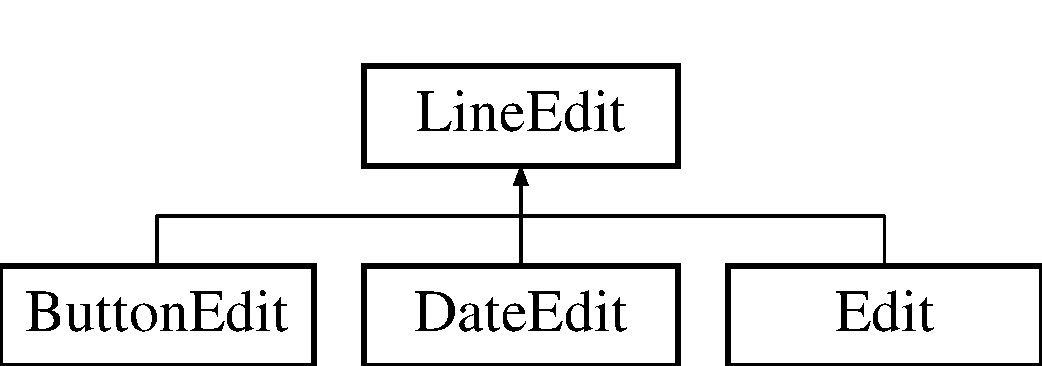
\includegraphics[height=2.000000cm]{classLineEdit}
\end{center}
\end{figure}
\subsection*{Public Slots}
\begin{DoxyCompactItemize}
\item 
void \hyperlink{classLineEdit_ad3cd1fe6bd62dfbd72e071054711015d}{isTouched} ()
\item 
void \hyperlink{classLineEdit_ae01737e586a9fc6f880c15885b7e8479}{checkNext} (const QString \&)
\end{DoxyCompactItemize}
\subsection*{Signals}
\begin{DoxyCompactItemize}
\item 
void \hyperlink{classLineEdit_a5d13e4462115bd039c90f38429a7de14}{widgetOpen} ()
\item 
void \hyperlink{classLineEdit_ad00eb1212a7343c7f80d65a19d23c4e0}{nextField} ()
\item 
void \hyperlink{classLineEdit_acb394b5ebd47db7a2fddf3ba3d57344e}{fieldEvent} (\hyperlink{structFgl_1_1Event}{Fgl::Event})
\item 
void \hyperlink{classLineEdit_afb721c2578c83bad5d35f84e069b615a}{error} (QString)
\item 
void \hyperlink{classLineEdit_a54187e66ebc1bdad7421e3b20b996444}{dropSuccess} ()
\end{DoxyCompactItemize}
\subsection*{Public Member Functions}
\begin{DoxyCompactItemize}
\item 
\hyperlink{classLineEdit_a0c54dc37150c2eea45af904a8146025a}{LineEdit} (QWidget $\ast$parent=0)
\item 
void \hyperlink{classLineEdit_a2f16adf255e3b0413579c3c689040afd}{setNoEntry} (bool ro)
\item 
bool \hyperlink{classLineEdit_aae4ac49369514ba569049214623f6dea}{noEntry} ()
\item 
void \hyperlink{classLineEdit_aee6f145415075ee47b730cbd26941f1b}{setAutoNext} (bool ro)
\item 
bool \hyperlink{classLineEdit_aca89c8a1aa943a93e68cd0a910f2331b}{autoNext} ()
\item 
void \hyperlink{classLineEdit_ac5c681c48927ade8548fd3293b614b78}{setRequired} (bool ro)
\item 
bool \hyperlink{classLineEdit_af82e35289d3464e9d161fd69cfdbbbe0}{required} ()
\item 
void \hyperlink{classLineEdit_afbe0dcdde72b9be055701f6a1bd0608b}{setCompress} (bool ro)
\item 
bool \hyperlink{classLineEdit_aac8fb7e5ef390627a71044b0ae8745bc}{compress} ()
\item 
void \hyperlink{classLineEdit_abcca038575cbc1ce186062f671763608}{setShift} (QString s)
\item 
QString \hyperlink{classLineEdit_a3d10f3933a882f6afef6383cb758191b}{shift} ()
\item 
void \hyperlink{classLineEdit_a8c0cb7cb1a2b0738db17ab3fad4b251b}{setSqlType} (QString)
\item 
QString \hyperlink{classLineEdit_afff2070683add5e2bc642cc58ae05a74}{sqlType} ()
\item 
\hyperlink{namespaceFgl_a221c9c0366d5227f8c27ca97308a691c}{Fgl::DataType} \hyperlink{classLineEdit_ac24782317d25afec4c02d74ed5892c99}{dataType} ()
\item 
const QValidator $\ast$ \hyperlink{classLineEdit_a7f6fef4035828aa9413b5d5763680adb}{getValidator} ()
\item 
void \hyperlink{classLineEdit_a52dde6d0059debb1730a029fceab64b7}{setTouchendEnabled} (bool t)
\item 
bool \hyperlink{classLineEdit_a7b733b195f9df2b7b495d030993868c6}{touched} ()
\item 
void \hyperlink{classLineEdit_a65785ee018716e1d1f3145070de82aba}{setDefaultValue} (QString def)
\item 
QString \hyperlink{classLineEdit_ab812bc7b7f6ff4df6f0978b2a10affca}{defaultValue} ()
\item 
void \hyperlink{classLineEdit_a28de25ae19583ad6446fd57f4d7d80a5}{setPicture} (QString pic)
\item 
QString \hyperlink{classLineEdit_afa2599d7285a22ead9fc92f8277a3f99}{picture} ()
\item 
void \hyperlink{classLineEdit_ab1d9a17ce52c3bceb98ef4536e107dbe}{setFormat} (QString f)
\item 
QString \hyperlink{classLineEdit_a748da55fa9586cd430c4ed68bf5f7219}{format} ()
\item 
void \hyperlink{classLineEdit_add02ad1ab2af8928e3245f44fa62c071}{check} ()
\end{DoxyCompactItemize}
\subsection*{Public Attributes}
\begin{DoxyCompactItemize}
\item 
QString \hyperlink{classLineEdit_ac7a4f4fcd5b7f40f66c47ff64d66f7ec}{sqlTabName}
\item 
QString \hyperlink{classLineEdit_a337f64c9e882f065b5771f9e2289784f}{name}
\item 
QString \hyperlink{classLineEdit_a18b45b2581575cf88489ab3a6f15281f}{colName}
\item 
int \hyperlink{classLineEdit_a8a3d3eb982e8a27cc6bdbf3664330bb4}{x}
\item 
int \hyperlink{classLineEdit_aa6005ddcc5167be3d2d3d73e869dd434}{y}
\item 
int \hyperlink{classLineEdit_a9ac1b912bc68696a166d681a5b86dbf2}{w}
\item 
bool \hyperlink{classLineEdit_a4769336d33259d543b795da2831fe4f7}{b\_\-denyFocus}
\end{DoxyCompactItemize}
\subsection*{Protected Member Functions}
\begin{DoxyCompactItemize}
\item 
void \hyperlink{classLineEdit_a4aea170d9ee45df41951a8565b4a8d9a}{dropEvent} (QDropEvent $\ast$)
\item 
void \hyperlink{classLineEdit_afa85c9e14cc728c93cfa848af50c2762}{dragEnterEvent} (QDragEnterEvent $\ast$)
\end{DoxyCompactItemize}
\subsection*{Private Attributes}
\begin{DoxyCompactItemize}
\item 
QString \hyperlink{classLineEdit_a662654e1d1126e311ba37ab357f90ef3}{qs\_\-sqlType}
\item 
bool \hyperlink{classLineEdit_a86b1ba413925186833fa1ffe1d08fe23}{b\_\-noEntry}
\item 
bool \hyperlink{classLineEdit_aa85bee848a5fcf91042127505f0d3686}{b\_\-autoNext}
\item 
bool \hyperlink{classLineEdit_a54067fa92f09cdde4c4f900333a1af5d}{b\_\-required}
\item 
bool \hyperlink{classLineEdit_afee15f7042521fb78ee568902aa8b603}{b\_\-compress}
\item 
QString \hyperlink{classLineEdit_ae554482e3fa80ec2695a79850b36bf1b}{qs\_\-shift}
\item 
const QValidator $\ast$ \hyperlink{classLineEdit_a4d9da17a0bc8380fdb22c4b197431d0a}{valid}
\item 
QString \hyperlink{classLineEdit_a73d2e143f00df406134a9e73ceba40af}{qs\_\-default}
\item 
QString \hyperlink{classLineEdit_aa7911a11a6d620f20248e968c093bd94}{qs\_\-picture}
\item 
QString \hyperlink{classLineEdit_ac06a746e3b29d84d14672e0931d1c457}{qs\_\-format}
\item 
\hyperlink{namespaceFgl_a221c9c0366d5227f8c27ca97308a691c}{Fgl::DataType} \hyperlink{classLineEdit_a7eafffbf2d586eac9c90f5d97fd89c6e}{dt\_\-dataType}
\end{DoxyCompactItemize}


\subsection{Detailed Description}


Definition at line 115 of file vwidgets.h.



\subsection{Constructor \& Destructor Documentation}
\hypertarget{classLineEdit_a0c54dc37150c2eea45af904a8146025a}{
\index{LineEdit@{LineEdit}!LineEdit@{LineEdit}}
\index{LineEdit@{LineEdit}!LineEdit@{LineEdit}}
\subsubsection[{LineEdit}]{\setlength{\rightskip}{0pt plus 5cm}LineEdit::LineEdit (
\begin{DoxyParamCaption}
\item[{QWidget $\ast$}]{parent = {\ttfamily 0}}
\end{DoxyParamCaption}
)}}
\label{classLineEdit_a0c54dc37150c2eea45af904a8146025a}


Definition at line 290 of file vwidgets.cpp.



\subsection{Member Function Documentation}
\hypertarget{classLineEdit_aca89c8a1aa943a93e68cd0a910f2331b}{
\index{LineEdit@{LineEdit}!autoNext@{autoNext}}
\index{autoNext@{autoNext}!LineEdit@{LineEdit}}
\subsubsection[{autoNext}]{\setlength{\rightskip}{0pt plus 5cm}bool LineEdit::autoNext (
\begin{DoxyParamCaption}
{}
\end{DoxyParamCaption}
)\hspace{0.3cm}{\ttfamily  \mbox{[}inline\mbox{]}}}}
\label{classLineEdit_aca89c8a1aa943a93e68cd0a910f2331b}


Definition at line 132 of file vwidgets.h.

\hypertarget{classLineEdit_add02ad1ab2af8928e3245f44fa62c071}{
\index{LineEdit@{LineEdit}!check@{check}}
\index{check@{check}!LineEdit@{LineEdit}}
\subsubsection[{check}]{\setlength{\rightskip}{0pt plus 5cm}void LineEdit::check (
\begin{DoxyParamCaption}
{}
\end{DoxyParamCaption}
)}}
\label{classLineEdit_add02ad1ab2af8928e3245f44fa62c071}


Definition at line 319 of file vwidgets.cpp.

\hypertarget{classLineEdit_ae01737e586a9fc6f880c15885b7e8479}{
\index{LineEdit@{LineEdit}!checkNext@{checkNext}}
\index{checkNext@{checkNext}!LineEdit@{LineEdit}}
\subsubsection[{checkNext}]{\setlength{\rightskip}{0pt plus 5cm}void LineEdit::checkNext (
\begin{DoxyParamCaption}
\item[{const QString \&}]{textr}
\end{DoxyParamCaption}
)\hspace{0.3cm}{\ttfamily  \mbox{[}slot\mbox{]}}}}
\label{classLineEdit_ae01737e586a9fc6f880c15885b7e8479}


Definition at line 385 of file vwidgets.cpp.

\hypertarget{classLineEdit_aac8fb7e5ef390627a71044b0ae8745bc}{
\index{LineEdit@{LineEdit}!compress@{compress}}
\index{compress@{compress}!LineEdit@{LineEdit}}
\subsubsection[{compress}]{\setlength{\rightskip}{0pt plus 5cm}bool LineEdit::compress (
\begin{DoxyParamCaption}
{}
\end{DoxyParamCaption}
)\hspace{0.3cm}{\ttfamily  \mbox{[}inline\mbox{]}}}}
\label{classLineEdit_aac8fb7e5ef390627a71044b0ae8745bc}


Definition at line 136 of file vwidgets.h.

\hypertarget{classLineEdit_ac24782317d25afec4c02d74ed5892c99}{
\index{LineEdit@{LineEdit}!dataType@{dataType}}
\index{dataType@{dataType}!LineEdit@{LineEdit}}
\subsubsection[{dataType}]{\setlength{\rightskip}{0pt plus 5cm}{\bf Fgl::DataType} LineEdit::dataType (
\begin{DoxyParamCaption}
{}
\end{DoxyParamCaption}
)\hspace{0.3cm}{\ttfamily  \mbox{[}inline\mbox{]}}}}
\label{classLineEdit_ac24782317d25afec4c02d74ed5892c99}


Definition at line 141 of file vwidgets.h.

\hypertarget{classLineEdit_ab812bc7b7f6ff4df6f0978b2a10affca}{
\index{LineEdit@{LineEdit}!defaultValue@{defaultValue}}
\index{defaultValue@{defaultValue}!LineEdit@{LineEdit}}
\subsubsection[{defaultValue}]{\setlength{\rightskip}{0pt plus 5cm}QString LineEdit::defaultValue (
\begin{DoxyParamCaption}
{}
\end{DoxyParamCaption}
)\hspace{0.3cm}{\ttfamily  \mbox{[}inline\mbox{]}}}}
\label{classLineEdit_ab812bc7b7f6ff4df6f0978b2a10affca}


Definition at line 146 of file vwidgets.h.

\hypertarget{classLineEdit_afa85c9e14cc728c93cfa848af50c2762}{
\index{LineEdit@{LineEdit}!dragEnterEvent@{dragEnterEvent}}
\index{dragEnterEvent@{dragEnterEvent}!LineEdit@{LineEdit}}
\subsubsection[{dragEnterEvent}]{\setlength{\rightskip}{0pt plus 5cm}void LineEdit::dragEnterEvent (
\begin{DoxyParamCaption}
\item[{QDragEnterEvent $\ast$}]{e}
\end{DoxyParamCaption}
)\hspace{0.3cm}{\ttfamily  \mbox{[}protected\mbox{]}}}}
\label{classLineEdit_afa85c9e14cc728c93cfa848af50c2762}


Definition at line 393 of file vwidgets.cpp.

\hypertarget{classLineEdit_a4aea170d9ee45df41951a8565b4a8d9a}{
\index{LineEdit@{LineEdit}!dropEvent@{dropEvent}}
\index{dropEvent@{dropEvent}!LineEdit@{LineEdit}}
\subsubsection[{dropEvent}]{\setlength{\rightskip}{0pt plus 5cm}void LineEdit::dropEvent (
\begin{DoxyParamCaption}
\item[{QDropEvent $\ast$}]{e}
\end{DoxyParamCaption}
)\hspace{0.3cm}{\ttfamily  \mbox{[}protected\mbox{]}}}}
\label{classLineEdit_a4aea170d9ee45df41951a8565b4a8d9a}


Definition at line 402 of file vwidgets.cpp.

\hypertarget{classLineEdit_a54187e66ebc1bdad7421e3b20b996444}{
\index{LineEdit@{LineEdit}!dropSuccess@{dropSuccess}}
\index{dropSuccess@{dropSuccess}!LineEdit@{LineEdit}}
\subsubsection[{dropSuccess}]{\setlength{\rightskip}{0pt plus 5cm}void LineEdit::dropSuccess (
\begin{DoxyParamCaption}
{}
\end{DoxyParamCaption}
)\hspace{0.3cm}{\ttfamily  \mbox{[}signal\mbox{]}}}}
\label{classLineEdit_a54187e66ebc1bdad7421e3b20b996444}
\hypertarget{classLineEdit_afb721c2578c83bad5d35f84e069b615a}{
\index{LineEdit@{LineEdit}!error@{error}}
\index{error@{error}!LineEdit@{LineEdit}}
\subsubsection[{error}]{\setlength{\rightskip}{0pt plus 5cm}void LineEdit::error (
\begin{DoxyParamCaption}
\item[{QString}]{}
\end{DoxyParamCaption}
)\hspace{0.3cm}{\ttfamily  \mbox{[}signal\mbox{]}}}}
\label{classLineEdit_afb721c2578c83bad5d35f84e069b615a}
\hypertarget{classLineEdit_acb394b5ebd47db7a2fddf3ba3d57344e}{
\index{LineEdit@{LineEdit}!fieldEvent@{fieldEvent}}
\index{fieldEvent@{fieldEvent}!LineEdit@{LineEdit}}
\subsubsection[{fieldEvent}]{\setlength{\rightskip}{0pt plus 5cm}void LineEdit::fieldEvent (
\begin{DoxyParamCaption}
\item[{{\bf Fgl::Event}}]{}
\end{DoxyParamCaption}
)\hspace{0.3cm}{\ttfamily  \mbox{[}signal\mbox{]}}}}
\label{classLineEdit_acb394b5ebd47db7a2fddf3ba3d57344e}
\hypertarget{classLineEdit_a748da55fa9586cd430c4ed68bf5f7219}{
\index{LineEdit@{LineEdit}!format@{format}}
\index{format@{format}!LineEdit@{LineEdit}}
\subsubsection[{format}]{\setlength{\rightskip}{0pt plus 5cm}QString LineEdit::format (
\begin{DoxyParamCaption}
{}
\end{DoxyParamCaption}
)\hspace{0.3cm}{\ttfamily  \mbox{[}inline\mbox{]}}}}
\label{classLineEdit_a748da55fa9586cd430c4ed68bf5f7219}


Definition at line 150 of file vwidgets.h.

\hypertarget{classLineEdit_a7f6fef4035828aa9413b5d5763680adb}{
\index{LineEdit@{LineEdit}!getValidator@{getValidator}}
\index{getValidator@{getValidator}!LineEdit@{LineEdit}}
\subsubsection[{getValidator}]{\setlength{\rightskip}{0pt plus 5cm}const QValidator$\ast$ LineEdit::getValidator (
\begin{DoxyParamCaption}
{}
\end{DoxyParamCaption}
)\hspace{0.3cm}{\ttfamily  \mbox{[}inline\mbox{]}}}}
\label{classLineEdit_a7f6fef4035828aa9413b5d5763680adb}


Definition at line 142 of file vwidgets.h.

\hypertarget{classLineEdit_ad3cd1fe6bd62dfbd72e071054711015d}{
\index{LineEdit@{LineEdit}!isTouched@{isTouched}}
\index{isTouched@{isTouched}!LineEdit@{LineEdit}}
\subsubsection[{isTouched}]{\setlength{\rightskip}{0pt plus 5cm}void LineEdit::isTouched (
\begin{DoxyParamCaption}
{}
\end{DoxyParamCaption}
)\hspace{0.3cm}{\ttfamily  \mbox{[}inline, slot\mbox{]}}}}
\label{classLineEdit_ad3cd1fe6bd62dfbd72e071054711015d}


Definition at line 174 of file vwidgets.h.

\hypertarget{classLineEdit_ad00eb1212a7343c7f80d65a19d23c4e0}{
\index{LineEdit@{LineEdit}!nextField@{nextField}}
\index{nextField@{nextField}!LineEdit@{LineEdit}}
\subsubsection[{nextField}]{\setlength{\rightskip}{0pt plus 5cm}void LineEdit::nextField (
\begin{DoxyParamCaption}
{}
\end{DoxyParamCaption}
)\hspace{0.3cm}{\ttfamily  \mbox{[}signal\mbox{]}}}}
\label{classLineEdit_ad00eb1212a7343c7f80d65a19d23c4e0}
\hypertarget{classLineEdit_aae4ac49369514ba569049214623f6dea}{
\index{LineEdit@{LineEdit}!noEntry@{noEntry}}
\index{noEntry@{noEntry}!LineEdit@{LineEdit}}
\subsubsection[{noEntry}]{\setlength{\rightskip}{0pt plus 5cm}bool LineEdit::noEntry (
\begin{DoxyParamCaption}
{}
\end{DoxyParamCaption}
)\hspace{0.3cm}{\ttfamily  \mbox{[}inline\mbox{]}}}}
\label{classLineEdit_aae4ac49369514ba569049214623f6dea}


Definition at line 130 of file vwidgets.h.

\hypertarget{classLineEdit_afa2599d7285a22ead9fc92f8277a3f99}{
\index{LineEdit@{LineEdit}!picture@{picture}}
\index{picture@{picture}!LineEdit@{LineEdit}}
\subsubsection[{picture}]{\setlength{\rightskip}{0pt plus 5cm}QString LineEdit::picture (
\begin{DoxyParamCaption}
{}
\end{DoxyParamCaption}
)\hspace{0.3cm}{\ttfamily  \mbox{[}inline\mbox{]}}}}
\label{classLineEdit_afa2599d7285a22ead9fc92f8277a3f99}


Definition at line 148 of file vwidgets.h.

\hypertarget{classLineEdit_af82e35289d3464e9d161fd69cfdbbbe0}{
\index{LineEdit@{LineEdit}!required@{required}}
\index{required@{required}!LineEdit@{LineEdit}}
\subsubsection[{required}]{\setlength{\rightskip}{0pt plus 5cm}bool LineEdit::required (
\begin{DoxyParamCaption}
{}
\end{DoxyParamCaption}
)\hspace{0.3cm}{\ttfamily  \mbox{[}inline\mbox{]}}}}
\label{classLineEdit_af82e35289d3464e9d161fd69cfdbbbe0}


Definition at line 134 of file vwidgets.h.

\hypertarget{classLineEdit_aee6f145415075ee47b730cbd26941f1b}{
\index{LineEdit@{LineEdit}!setAutoNext@{setAutoNext}}
\index{setAutoNext@{setAutoNext}!LineEdit@{LineEdit}}
\subsubsection[{setAutoNext}]{\setlength{\rightskip}{0pt plus 5cm}void LineEdit::setAutoNext (
\begin{DoxyParamCaption}
\item[{bool}]{ro}
\end{DoxyParamCaption}
)\hspace{0.3cm}{\ttfamily  \mbox{[}inline\mbox{]}}}}
\label{classLineEdit_aee6f145415075ee47b730cbd26941f1b}


Definition at line 131 of file vwidgets.h.

\hypertarget{classLineEdit_afbe0dcdde72b9be055701f6a1bd0608b}{
\index{LineEdit@{LineEdit}!setCompress@{setCompress}}
\index{setCompress@{setCompress}!LineEdit@{LineEdit}}
\subsubsection[{setCompress}]{\setlength{\rightskip}{0pt plus 5cm}void LineEdit::setCompress (
\begin{DoxyParamCaption}
\item[{bool}]{ro}
\end{DoxyParamCaption}
)\hspace{0.3cm}{\ttfamily  \mbox{[}inline\mbox{]}}}}
\label{classLineEdit_afbe0dcdde72b9be055701f6a1bd0608b}


Definition at line 135 of file vwidgets.h.

\hypertarget{classLineEdit_a65785ee018716e1d1f3145070de82aba}{
\index{LineEdit@{LineEdit}!setDefaultValue@{setDefaultValue}}
\index{setDefaultValue@{setDefaultValue}!LineEdit@{LineEdit}}
\subsubsection[{setDefaultValue}]{\setlength{\rightskip}{0pt plus 5cm}void LineEdit::setDefaultValue (
\begin{DoxyParamCaption}
\item[{QString}]{def}
\end{DoxyParamCaption}
)\hspace{0.3cm}{\ttfamily  \mbox{[}inline\mbox{]}}}}
\label{classLineEdit_a65785ee018716e1d1f3145070de82aba}


Definition at line 145 of file vwidgets.h.

\hypertarget{classLineEdit_ab1d9a17ce52c3bceb98ef4536e107dbe}{
\index{LineEdit@{LineEdit}!setFormat@{setFormat}}
\index{setFormat@{setFormat}!LineEdit@{LineEdit}}
\subsubsection[{setFormat}]{\setlength{\rightskip}{0pt plus 5cm}void LineEdit::setFormat (
\begin{DoxyParamCaption}
\item[{QString}]{f}
\end{DoxyParamCaption}
)\hspace{0.3cm}{\ttfamily  \mbox{[}inline\mbox{]}}}}
\label{classLineEdit_ab1d9a17ce52c3bceb98ef4536e107dbe}


Definition at line 149 of file vwidgets.h.

\hypertarget{classLineEdit_a2f16adf255e3b0413579c3c689040afd}{
\index{LineEdit@{LineEdit}!setNoEntry@{setNoEntry}}
\index{setNoEntry@{setNoEntry}!LineEdit@{LineEdit}}
\subsubsection[{setNoEntry}]{\setlength{\rightskip}{0pt plus 5cm}void LineEdit::setNoEntry (
\begin{DoxyParamCaption}
\item[{bool}]{ro}
\end{DoxyParamCaption}
)}}
\label{classLineEdit_a2f16adf255e3b0413579c3c689040afd}


Definition at line 336 of file vwidgets.cpp.

\hypertarget{classLineEdit_a28de25ae19583ad6446fd57f4d7d80a5}{
\index{LineEdit@{LineEdit}!setPicture@{setPicture}}
\index{setPicture@{setPicture}!LineEdit@{LineEdit}}
\subsubsection[{setPicture}]{\setlength{\rightskip}{0pt plus 5cm}void LineEdit::setPicture (
\begin{DoxyParamCaption}
\item[{QString}]{pic}
\end{DoxyParamCaption}
)\hspace{0.3cm}{\ttfamily  \mbox{[}inline\mbox{]}}}}
\label{classLineEdit_a28de25ae19583ad6446fd57f4d7d80a5}


Definition at line 147 of file vwidgets.h.

\hypertarget{classLineEdit_ac5c681c48927ade8548fd3293b614b78}{
\index{LineEdit@{LineEdit}!setRequired@{setRequired}}
\index{setRequired@{setRequired}!LineEdit@{LineEdit}}
\subsubsection[{setRequired}]{\setlength{\rightskip}{0pt plus 5cm}void LineEdit::setRequired (
\begin{DoxyParamCaption}
\item[{bool}]{ro}
\end{DoxyParamCaption}
)\hspace{0.3cm}{\ttfamily  \mbox{[}inline\mbox{]}}}}
\label{classLineEdit_ac5c681c48927ade8548fd3293b614b78}


Definition at line 133 of file vwidgets.h.

\hypertarget{classLineEdit_abcca038575cbc1ce186062f671763608}{
\index{LineEdit@{LineEdit}!setShift@{setShift}}
\index{setShift@{setShift}!LineEdit@{LineEdit}}
\subsubsection[{setShift}]{\setlength{\rightskip}{0pt plus 5cm}void LineEdit::setShift (
\begin{DoxyParamCaption}
\item[{QString}]{s}
\end{DoxyParamCaption}
)\hspace{0.3cm}{\ttfamily  \mbox{[}inline\mbox{]}}}}
\label{classLineEdit_abcca038575cbc1ce186062f671763608}


Definition at line 137 of file vwidgets.h.

\hypertarget{classLineEdit_a8c0cb7cb1a2b0738db17ab3fad4b251b}{
\index{LineEdit@{LineEdit}!setSqlType@{setSqlType}}
\index{setSqlType@{setSqlType}!LineEdit@{LineEdit}}
\subsubsection[{setSqlType}]{\setlength{\rightskip}{0pt plus 5cm}void LineEdit::setSqlType (
\begin{DoxyParamCaption}
\item[{QString}]{sqlType}
\end{DoxyParamCaption}
)}}
\label{classLineEdit_a8c0cb7cb1a2b0738db17ab3fad4b251b}


Definition at line 350 of file vwidgets.cpp.

\hypertarget{classLineEdit_a52dde6d0059debb1730a029fceab64b7}{
\index{LineEdit@{LineEdit}!setTouchendEnabled@{setTouchendEnabled}}
\index{setTouchendEnabled@{setTouchendEnabled}!LineEdit@{LineEdit}}
\subsubsection[{setTouchendEnabled}]{\setlength{\rightskip}{0pt plus 5cm}void LineEdit::setTouchendEnabled (
\begin{DoxyParamCaption}
\item[{bool}]{t}
\end{DoxyParamCaption}
)\hspace{0.3cm}{\ttfamily  \mbox{[}inline\mbox{]}}}}
\label{classLineEdit_a52dde6d0059debb1730a029fceab64b7}


Definition at line 143 of file vwidgets.h.

\hypertarget{classLineEdit_a3d10f3933a882f6afef6383cb758191b}{
\index{LineEdit@{LineEdit}!shift@{shift}}
\index{shift@{shift}!LineEdit@{LineEdit}}
\subsubsection[{shift}]{\setlength{\rightskip}{0pt plus 5cm}QString LineEdit::shift (
\begin{DoxyParamCaption}
{}
\end{DoxyParamCaption}
)\hspace{0.3cm}{\ttfamily  \mbox{[}inline\mbox{]}}}}
\label{classLineEdit_a3d10f3933a882f6afef6383cb758191b}


Definition at line 138 of file vwidgets.h.

\hypertarget{classLineEdit_afff2070683add5e2bc642cc58ae05a74}{
\index{LineEdit@{LineEdit}!sqlType@{sqlType}}
\index{sqlType@{sqlType}!LineEdit@{LineEdit}}
\subsubsection[{sqlType}]{\setlength{\rightskip}{0pt plus 5cm}QString LineEdit::sqlType (
\begin{DoxyParamCaption}
{}
\end{DoxyParamCaption}
)\hspace{0.3cm}{\ttfamily  \mbox{[}inline\mbox{]}}}}
\label{classLineEdit_afff2070683add5e2bc642cc58ae05a74}


Definition at line 140 of file vwidgets.h.

\hypertarget{classLineEdit_a7b733b195f9df2b7b495d030993868c6}{
\index{LineEdit@{LineEdit}!touched@{touched}}
\index{touched@{touched}!LineEdit@{LineEdit}}
\subsubsection[{touched}]{\setlength{\rightskip}{0pt plus 5cm}bool LineEdit::touched (
\begin{DoxyParamCaption}
{}
\end{DoxyParamCaption}
)\hspace{0.3cm}{\ttfamily  \mbox{[}inline\mbox{]}}}}
\label{classLineEdit_a7b733b195f9df2b7b495d030993868c6}


Definition at line 144 of file vwidgets.h.

\hypertarget{classLineEdit_a5d13e4462115bd039c90f38429a7de14}{
\index{LineEdit@{LineEdit}!widgetOpen@{widgetOpen}}
\index{widgetOpen@{widgetOpen}!LineEdit@{LineEdit}}
\subsubsection[{widgetOpen}]{\setlength{\rightskip}{0pt plus 5cm}void LineEdit::widgetOpen (
\begin{DoxyParamCaption}
{}
\end{DoxyParamCaption}
)\hspace{0.3cm}{\ttfamily  \mbox{[}signal\mbox{]}}}}
\label{classLineEdit_a5d13e4462115bd039c90f38429a7de14}


\subsection{Member Data Documentation}
\hypertarget{classLineEdit_aa85bee848a5fcf91042127505f0d3686}{
\index{LineEdit@{LineEdit}!b\_\-autoNext@{b\_\-autoNext}}
\index{b\_\-autoNext@{b\_\-autoNext}!LineEdit@{LineEdit}}
\subsubsection[{b\_\-autoNext}]{\setlength{\rightskip}{0pt plus 5cm}bool {\bf LineEdit::b\_\-autoNext}\hspace{0.3cm}{\ttfamily  \mbox{[}private\mbox{]}}}}
\label{classLineEdit_aa85bee848a5fcf91042127505f0d3686}


Definition at line 163 of file vwidgets.h.

\hypertarget{classLineEdit_afee15f7042521fb78ee568902aa8b603}{
\index{LineEdit@{LineEdit}!b\_\-compress@{b\_\-compress}}
\index{b\_\-compress@{b\_\-compress}!LineEdit@{LineEdit}}
\subsubsection[{b\_\-compress}]{\setlength{\rightskip}{0pt plus 5cm}bool {\bf LineEdit::b\_\-compress}\hspace{0.3cm}{\ttfamily  \mbox{[}private\mbox{]}}}}
\label{classLineEdit_afee15f7042521fb78ee568902aa8b603}


Definition at line 165 of file vwidgets.h.

\hypertarget{classLineEdit_a4769336d33259d543b795da2831fe4f7}{
\index{LineEdit@{LineEdit}!b\_\-denyFocus@{b\_\-denyFocus}}
\index{b\_\-denyFocus@{b\_\-denyFocus}!LineEdit@{LineEdit}}
\subsubsection[{b\_\-denyFocus}]{\setlength{\rightskip}{0pt plus 5cm}bool {\bf LineEdit::b\_\-denyFocus}}}
\label{classLineEdit_a4769336d33259d543b795da2831fe4f7}


Definition at line 153 of file vwidgets.h.

\hypertarget{classLineEdit_a86b1ba413925186833fa1ffe1d08fe23}{
\index{LineEdit@{LineEdit}!b\_\-noEntry@{b\_\-noEntry}}
\index{b\_\-noEntry@{b\_\-noEntry}!LineEdit@{LineEdit}}
\subsubsection[{b\_\-noEntry}]{\setlength{\rightskip}{0pt plus 5cm}bool {\bf LineEdit::b\_\-noEntry}\hspace{0.3cm}{\ttfamily  \mbox{[}private\mbox{]}}}}
\label{classLineEdit_a86b1ba413925186833fa1ffe1d08fe23}


Definition at line 162 of file vwidgets.h.

\hypertarget{classLineEdit_a54067fa92f09cdde4c4f900333a1af5d}{
\index{LineEdit@{LineEdit}!b\_\-required@{b\_\-required}}
\index{b\_\-required@{b\_\-required}!LineEdit@{LineEdit}}
\subsubsection[{b\_\-required}]{\setlength{\rightskip}{0pt plus 5cm}bool {\bf LineEdit::b\_\-required}\hspace{0.3cm}{\ttfamily  \mbox{[}private\mbox{]}}}}
\label{classLineEdit_a54067fa92f09cdde4c4f900333a1af5d}


Definition at line 164 of file vwidgets.h.

\hypertarget{classLineEdit_a18b45b2581575cf88489ab3a6f15281f}{
\index{LineEdit@{LineEdit}!colName@{colName}}
\index{colName@{colName}!LineEdit@{LineEdit}}
\subsubsection[{colName}]{\setlength{\rightskip}{0pt plus 5cm}QString {\bf LineEdit::colName}}}
\label{classLineEdit_a18b45b2581575cf88489ab3a6f15281f}


Definition at line 123 of file vwidgets.h.

\hypertarget{classLineEdit_a7eafffbf2d586eac9c90f5d97fd89c6e}{
\index{LineEdit@{LineEdit}!dt\_\-dataType@{dt\_\-dataType}}
\index{dt\_\-dataType@{dt\_\-dataType}!LineEdit@{LineEdit}}
\subsubsection[{dt\_\-dataType}]{\setlength{\rightskip}{0pt plus 5cm}{\bf Fgl::DataType} {\bf LineEdit::dt\_\-dataType}\hspace{0.3cm}{\ttfamily  \mbox{[}private\mbox{]}}}}
\label{classLineEdit_a7eafffbf2d586eac9c90f5d97fd89c6e}


Definition at line 171 of file vwidgets.h.

\hypertarget{classLineEdit_a337f64c9e882f065b5771f9e2289784f}{
\index{LineEdit@{LineEdit}!name@{name}}
\index{name@{name}!LineEdit@{LineEdit}}
\subsubsection[{name}]{\setlength{\rightskip}{0pt plus 5cm}QString {\bf LineEdit::name}}}
\label{classLineEdit_a337f64c9e882f065b5771f9e2289784f}


Definition at line 122 of file vwidgets.h.

\hypertarget{classLineEdit_a73d2e143f00df406134a9e73ceba40af}{
\index{LineEdit@{LineEdit}!qs\_\-default@{qs\_\-default}}
\index{qs\_\-default@{qs\_\-default}!LineEdit@{LineEdit}}
\subsubsection[{qs\_\-default}]{\setlength{\rightskip}{0pt plus 5cm}QString {\bf LineEdit::qs\_\-default}\hspace{0.3cm}{\ttfamily  \mbox{[}private\mbox{]}}}}
\label{classLineEdit_a73d2e143f00df406134a9e73ceba40af}


Definition at line 168 of file vwidgets.h.

\hypertarget{classLineEdit_ac06a746e3b29d84d14672e0931d1c457}{
\index{LineEdit@{LineEdit}!qs\_\-format@{qs\_\-format}}
\index{qs\_\-format@{qs\_\-format}!LineEdit@{LineEdit}}
\subsubsection[{qs\_\-format}]{\setlength{\rightskip}{0pt plus 5cm}QString {\bf LineEdit::qs\_\-format}\hspace{0.3cm}{\ttfamily  \mbox{[}private\mbox{]}}}}
\label{classLineEdit_ac06a746e3b29d84d14672e0931d1c457}


Definition at line 170 of file vwidgets.h.

\hypertarget{classLineEdit_aa7911a11a6d620f20248e968c093bd94}{
\index{LineEdit@{LineEdit}!qs\_\-picture@{qs\_\-picture}}
\index{qs\_\-picture@{qs\_\-picture}!LineEdit@{LineEdit}}
\subsubsection[{qs\_\-picture}]{\setlength{\rightskip}{0pt plus 5cm}QString {\bf LineEdit::qs\_\-picture}\hspace{0.3cm}{\ttfamily  \mbox{[}private\mbox{]}}}}
\label{classLineEdit_aa7911a11a6d620f20248e968c093bd94}


Definition at line 169 of file vwidgets.h.

\hypertarget{classLineEdit_ae554482e3fa80ec2695a79850b36bf1b}{
\index{LineEdit@{LineEdit}!qs\_\-shift@{qs\_\-shift}}
\index{qs\_\-shift@{qs\_\-shift}!LineEdit@{LineEdit}}
\subsubsection[{qs\_\-shift}]{\setlength{\rightskip}{0pt plus 5cm}QString {\bf LineEdit::qs\_\-shift}\hspace{0.3cm}{\ttfamily  \mbox{[}private\mbox{]}}}}
\label{classLineEdit_ae554482e3fa80ec2695a79850b36bf1b}


Definition at line 166 of file vwidgets.h.

\hypertarget{classLineEdit_a662654e1d1126e311ba37ab357f90ef3}{
\index{LineEdit@{LineEdit}!qs\_\-sqlType@{qs\_\-sqlType}}
\index{qs\_\-sqlType@{qs\_\-sqlType}!LineEdit@{LineEdit}}
\subsubsection[{qs\_\-sqlType}]{\setlength{\rightskip}{0pt plus 5cm}QString {\bf LineEdit::qs\_\-sqlType}\hspace{0.3cm}{\ttfamily  \mbox{[}private\mbox{]}}}}
\label{classLineEdit_a662654e1d1126e311ba37ab357f90ef3}


Definition at line 161 of file vwidgets.h.

\hypertarget{classLineEdit_ac7a4f4fcd5b7f40f66c47ff64d66f7ec}{
\index{LineEdit@{LineEdit}!sqlTabName@{sqlTabName}}
\index{sqlTabName@{sqlTabName}!LineEdit@{LineEdit}}
\subsubsection[{sqlTabName}]{\setlength{\rightskip}{0pt plus 5cm}QString {\bf LineEdit::sqlTabName}}}
\label{classLineEdit_ac7a4f4fcd5b7f40f66c47ff64d66f7ec}


Definition at line 121 of file vwidgets.h.

\hypertarget{classLineEdit_a4d9da17a0bc8380fdb22c4b197431d0a}{
\index{LineEdit@{LineEdit}!valid@{valid}}
\index{valid@{valid}!LineEdit@{LineEdit}}
\subsubsection[{valid}]{\setlength{\rightskip}{0pt plus 5cm}const QValidator$\ast$ {\bf LineEdit::valid}\hspace{0.3cm}{\ttfamily  \mbox{[}private\mbox{]}}}}
\label{classLineEdit_a4d9da17a0bc8380fdb22c4b197431d0a}


Definition at line 167 of file vwidgets.h.

\hypertarget{classLineEdit_a9ac1b912bc68696a166d681a5b86dbf2}{
\index{LineEdit@{LineEdit}!w@{w}}
\index{w@{w}!LineEdit@{LineEdit}}
\subsubsection[{w}]{\setlength{\rightskip}{0pt plus 5cm}int {\bf LineEdit::w}}}
\label{classLineEdit_a9ac1b912bc68696a166d681a5b86dbf2}


Definition at line 126 of file vwidgets.h.

\hypertarget{classLineEdit_a8a3d3eb982e8a27cc6bdbf3664330bb4}{
\index{LineEdit@{LineEdit}!x@{x}}
\index{x@{x}!LineEdit@{LineEdit}}
\subsubsection[{x}]{\setlength{\rightskip}{0pt plus 5cm}int {\bf LineEdit::x}}}
\label{classLineEdit_a8a3d3eb982e8a27cc6bdbf3664330bb4}


Definition at line 124 of file vwidgets.h.

\hypertarget{classLineEdit_aa6005ddcc5167be3d2d3d73e869dd434}{
\index{LineEdit@{LineEdit}!y@{y}}
\index{y@{y}!LineEdit@{LineEdit}}
\subsubsection[{y}]{\setlength{\rightskip}{0pt plus 5cm}int {\bf LineEdit::y}}}
\label{classLineEdit_aa6005ddcc5167be3d2d3d73e869dd434}


Definition at line 125 of file vwidgets.h.



The documentation for this class was generated from the following files:\begin{DoxyCompactItemize}
\item 
/e/ms/QT/models/\hyperlink{vwidgets_8h}{vwidgets.h}\item 
/e/ms/QT/models/\hyperlink{vwidgets_8cpp}{vwidgets.cpp}\end{DoxyCompactItemize}

\hypertarget{classLineEditDelegate}{
\section{LineEditDelegate Class Reference}
\label{classLineEditDelegate}\index{LineEditDelegate@{LineEditDelegate}}
}


{\ttfamily \#include $<$table.h$>$}

\subsection*{Signals}
\begin{DoxyCompactItemize}
\item 
void \hyperlink{classLineEditDelegate_aef453ff10ab9068948696442b9c2a867}{fieldEvent} (\hyperlink{structFgl_1_1Event}{Fgl::Event}, QWidget $\ast$)
\end{DoxyCompactItemize}
\subsection*{Public Member Functions}
\begin{DoxyCompactItemize}
\item 
\hyperlink{classLineEditDelegate_ab418c36b7c2603193b1365e6d43b4f8f}{LineEditDelegate} (QObject $\ast$parent=0)
\item 
\hyperlink{classLineEditDelegate_ade4fd9d641f292561e65488b1f50d2b0}{LineEditDelegate} (QDomElement, QObject $\ast$parent=0)
\item 
QWidget $\ast$ \hyperlink{classLineEditDelegate_a0134697582deea5baf2627b075e08189}{createEditor} (QWidget $\ast$parent, const QStyleOptionViewItem \&option, const QModelIndex \&index) const 
\item 
void \hyperlink{classLineEditDelegate_a7084c71313b96297c32ecf69e4c52fe0}{setEditorData} (QWidget $\ast$editor, const QModelIndex \&index) const 
\item 
void \hyperlink{classLineEditDelegate_add0abb09725ff1b794825cc428ec36b3}{setModelData} (QWidget $\ast$editor, QAbstractItemModel $\ast$model, const QModelIndex \&index) const 
\item 
void \hyperlink{classLineEditDelegate_a543ae4345264f2e17d75d80c6dcf9f41}{updateEditorGeometry} (QWidget $\ast$editor, const QStyleOptionViewItem \&option, const QModelIndex \&index) const 
\item 
QSize \hyperlink{classLineEditDelegate_a35ced057564e0e83f1cee748c0e4f8c0}{sizeHint} (const QStyleOptionViewItem \&option, const QModelIndex \&index) const 
\item 
void \hyperlink{classLineEditDelegate_a70f070297a44835836592b2dc7e9b38a}{setForm} (QWidget $\ast$form)
\item 
void \hyperlink{classLineEditDelegate_a4aca4a31277cbb989436840eb7371c6e}{setColumn} (int c)
\item 
int \hyperlink{classLineEditDelegate_a1d6c0bec6f2650cd4b6893c7e5c08480}{column} ()
\item 
bool \hyperlink{classLineEditDelegate_a72fc91aa30d6afb7264bd07c356788d0}{readOnly} ()
\end{DoxyCompactItemize}
\subsection*{Public Attributes}
\begin{DoxyCompactItemize}
\item 
QSize $\ast$ \hyperlink{classLineEditDelegate_ace648742ec01e245e35b39261383ae89}{fieldSize}
\item 
QWidget $\ast$ \hyperlink{classLineEditDelegate_a16d00d8e62e3c89978d07adcffa007c9}{qw\_\-editor}
\end{DoxyCompactItemize}
\subsection*{Protected Member Functions}
\begin{DoxyCompactItemize}
\item 
bool \hyperlink{classLineEditDelegate_acc5efdbc01898262cc1050dc696aad6a}{eventFilter} (QObject $\ast$editor, QEvent $\ast$event)
\end{DoxyCompactItemize}
\subsection*{Private Attributes}
\begin{DoxyCompactItemize}
\item 
QWidget $\ast$ \hyperlink{classLineEditDelegate_a2f504917f4de35dd8f400d8d696bdc1d}{p\_\-fglform}
\item 
QDomElement \hyperlink{classLineEditDelegate_aa635e6dd4afb8971b6d85db420c16773}{formElement}
\item 
QString \hyperlink{classLineEditDelegate_ad734b27bd24f9eebab7dc0b0a70897a7}{qs\_\-text}
\item 
bool \hyperlink{classLineEditDelegate_ae056ae674734bac2b666e31071568fbd}{b\_\-readOnly}
\item 
int \hyperlink{classLineEditDelegate_a8484d34acb269d70d28e3ccaa98c8a49}{i\_\-column}
\end{DoxyCompactItemize}


\subsection{Detailed Description}


Definition at line 199 of file table.h.



\subsection{Constructor \& Destructor Documentation}
\hypertarget{classLineEditDelegate_ab418c36b7c2603193b1365e6d43b4f8f}{
\index{LineEditDelegate@{LineEditDelegate}!LineEditDelegate@{LineEditDelegate}}
\index{LineEditDelegate@{LineEditDelegate}!LineEditDelegate@{LineEditDelegate}}
\subsubsection[{LineEditDelegate}]{\setlength{\rightskip}{0pt plus 5cm}LineEditDelegate::LineEditDelegate (
\begin{DoxyParamCaption}
\item[{QObject $\ast$}]{parent = {\ttfamily 0}}
\end{DoxyParamCaption}
)}}
\label{classLineEditDelegate_ab418c36b7c2603193b1365e6d43b4f8f}


Definition at line 1141 of file table.cpp.

\hypertarget{classLineEditDelegate_ade4fd9d641f292561e65488b1f50d2b0}{
\index{LineEditDelegate@{LineEditDelegate}!LineEditDelegate@{LineEditDelegate}}
\index{LineEditDelegate@{LineEditDelegate}!LineEditDelegate@{LineEditDelegate}}
\subsubsection[{LineEditDelegate}]{\setlength{\rightskip}{0pt plus 5cm}LineEditDelegate::LineEditDelegate (
\begin{DoxyParamCaption}
\item[{QDomElement}]{formElement, }
\item[{QObject $\ast$}]{parent = {\ttfamily 0}}
\end{DoxyParamCaption}
)}}
\label{classLineEditDelegate_ade4fd9d641f292561e65488b1f50d2b0}


Definition at line 1147 of file table.cpp.



\subsection{Member Function Documentation}
\hypertarget{classLineEditDelegate_a1d6c0bec6f2650cd4b6893c7e5c08480}{
\index{LineEditDelegate@{LineEditDelegate}!column@{column}}
\index{column@{column}!LineEditDelegate@{LineEditDelegate}}
\subsubsection[{column}]{\setlength{\rightskip}{0pt plus 5cm}int LineEditDelegate::column (
\begin{DoxyParamCaption}
{}
\end{DoxyParamCaption}
)\hspace{0.3cm}{\ttfamily  \mbox{[}inline\mbox{]}}}}
\label{classLineEditDelegate_a1d6c0bec6f2650cd4b6893c7e5c08480}


Definition at line 222 of file table.h.

\hypertarget{classLineEditDelegate_a0134697582deea5baf2627b075e08189}{
\index{LineEditDelegate@{LineEditDelegate}!createEditor@{createEditor}}
\index{createEditor@{createEditor}!LineEditDelegate@{LineEditDelegate}}
\subsubsection[{createEditor}]{\setlength{\rightskip}{0pt plus 5cm}QWidget $\ast$ LineEditDelegate::createEditor (
\begin{DoxyParamCaption}
\item[{QWidget $\ast$}]{parent, }
\item[{const QStyleOptionViewItem \&}]{option, }
\item[{const QModelIndex \&}]{index}
\end{DoxyParamCaption}
) const}}
\label{classLineEditDelegate_a0134697582deea5baf2627b075e08189}


Definition at line 1179 of file table.cpp.

\hypertarget{classLineEditDelegate_acc5efdbc01898262cc1050dc696aad6a}{
\index{LineEditDelegate@{LineEditDelegate}!eventFilter@{eventFilter}}
\index{eventFilter@{eventFilter}!LineEditDelegate@{LineEditDelegate}}
\subsubsection[{eventFilter}]{\setlength{\rightskip}{0pt plus 5cm}bool LineEditDelegate::eventFilter (
\begin{DoxyParamCaption}
\item[{QObject $\ast$}]{editor, }
\item[{QEvent $\ast$}]{event}
\end{DoxyParamCaption}
)\hspace{0.3cm}{\ttfamily  \mbox{[}protected\mbox{]}}}}
\label{classLineEditDelegate_acc5efdbc01898262cc1050dc696aad6a}


Definition at line 1235 of file table.cpp.

\hypertarget{classLineEditDelegate_aef453ff10ab9068948696442b9c2a867}{
\index{LineEditDelegate@{LineEditDelegate}!fieldEvent@{fieldEvent}}
\index{fieldEvent@{fieldEvent}!LineEditDelegate@{LineEditDelegate}}
\subsubsection[{fieldEvent}]{\setlength{\rightskip}{0pt plus 5cm}void LineEditDelegate::fieldEvent (
\begin{DoxyParamCaption}
\item[{{\bf Fgl::Event}}]{, }
\item[{QWidget $\ast$}]{}
\end{DoxyParamCaption}
)\hspace{0.3cm}{\ttfamily  \mbox{[}signal\mbox{]}}}}
\label{classLineEditDelegate_aef453ff10ab9068948696442b9c2a867}
\hypertarget{classLineEditDelegate_a72fc91aa30d6afb7264bd07c356788d0}{
\index{LineEditDelegate@{LineEditDelegate}!readOnly@{readOnly}}
\index{readOnly@{readOnly}!LineEditDelegate@{LineEditDelegate}}
\subsubsection[{readOnly}]{\setlength{\rightskip}{0pt plus 5cm}bool LineEditDelegate::readOnly (
\begin{DoxyParamCaption}
{}
\end{DoxyParamCaption}
)\hspace{0.3cm}{\ttfamily  \mbox{[}inline\mbox{]}}}}
\label{classLineEditDelegate_a72fc91aa30d6afb7264bd07c356788d0}


Definition at line 223 of file table.h.

\hypertarget{classLineEditDelegate_a4aca4a31277cbb989436840eb7371c6e}{
\index{LineEditDelegate@{LineEditDelegate}!setColumn@{setColumn}}
\index{setColumn@{setColumn}!LineEditDelegate@{LineEditDelegate}}
\subsubsection[{setColumn}]{\setlength{\rightskip}{0pt plus 5cm}void LineEditDelegate::setColumn (
\begin{DoxyParamCaption}
\item[{int}]{c}
\end{DoxyParamCaption}
)\hspace{0.3cm}{\ttfamily  \mbox{[}inline\mbox{]}}}}
\label{classLineEditDelegate_a4aca4a31277cbb989436840eb7371c6e}


Definition at line 221 of file table.h.

\hypertarget{classLineEditDelegate_a7084c71313b96297c32ecf69e4c52fe0}{
\index{LineEditDelegate@{LineEditDelegate}!setEditorData@{setEditorData}}
\index{setEditorData@{setEditorData}!LineEditDelegate@{LineEditDelegate}}
\subsubsection[{setEditorData}]{\setlength{\rightskip}{0pt plus 5cm}void LineEditDelegate::setEditorData (
\begin{DoxyParamCaption}
\item[{QWidget $\ast$}]{editor, }
\item[{const QModelIndex \&}]{index}
\end{DoxyParamCaption}
) const}}
\label{classLineEditDelegate_a7084c71313b96297c32ecf69e4c52fe0}


Definition at line 1203 of file table.cpp.

\hypertarget{classLineEditDelegate_a70f070297a44835836592b2dc7e9b38a}{
\index{LineEditDelegate@{LineEditDelegate}!setForm@{setForm}}
\index{setForm@{setForm}!LineEditDelegate@{LineEditDelegate}}
\subsubsection[{setForm}]{\setlength{\rightskip}{0pt plus 5cm}void LineEditDelegate::setForm (
\begin{DoxyParamCaption}
\item[{QWidget $\ast$}]{form}
\end{DoxyParamCaption}
)}}
\label{classLineEditDelegate_a70f070297a44835836592b2dc7e9b38a}


Definition at line 1228 of file table.cpp.

\hypertarget{classLineEditDelegate_add0abb09725ff1b794825cc428ec36b3}{
\index{LineEditDelegate@{LineEditDelegate}!setModelData@{setModelData}}
\index{setModelData@{setModelData}!LineEditDelegate@{LineEditDelegate}}
\subsubsection[{setModelData}]{\setlength{\rightskip}{0pt plus 5cm}void LineEditDelegate::setModelData (
\begin{DoxyParamCaption}
\item[{QWidget $\ast$}]{editor, }
\item[{QAbstractItemModel $\ast$}]{model, }
\item[{const QModelIndex \&}]{index}
\end{DoxyParamCaption}
) const}}
\label{classLineEditDelegate_add0abb09725ff1b794825cc428ec36b3}


Definition at line 1212 of file table.cpp.

\hypertarget{classLineEditDelegate_a35ced057564e0e83f1cee748c0e4f8c0}{
\index{LineEditDelegate@{LineEditDelegate}!sizeHint@{sizeHint}}
\index{sizeHint@{sizeHint}!LineEditDelegate@{LineEditDelegate}}
\subsubsection[{sizeHint}]{\setlength{\rightskip}{0pt plus 5cm}QSize LineEditDelegate::sizeHint (
\begin{DoxyParamCaption}
\item[{const QStyleOptionViewItem \&}]{option, }
\item[{const QModelIndex \&}]{index}
\end{DoxyParamCaption}
) const}}
\label{classLineEditDelegate_a35ced057564e0e83f1cee748c0e4f8c0}


Definition at line 1164 of file table.cpp.

\hypertarget{classLineEditDelegate_a543ae4345264f2e17d75d80c6dcf9f41}{
\index{LineEditDelegate@{LineEditDelegate}!updateEditorGeometry@{updateEditorGeometry}}
\index{updateEditorGeometry@{updateEditorGeometry}!LineEditDelegate@{LineEditDelegate}}
\subsubsection[{updateEditorGeometry}]{\setlength{\rightskip}{0pt plus 5cm}void LineEditDelegate::updateEditorGeometry (
\begin{DoxyParamCaption}
\item[{QWidget $\ast$}]{editor, }
\item[{const QStyleOptionViewItem \&}]{option, }
\item[{const QModelIndex \&}]{index}
\end{DoxyParamCaption}
) const}}
\label{classLineEditDelegate_a543ae4345264f2e17d75d80c6dcf9f41}


Definition at line 1222 of file table.cpp.



\subsection{Member Data Documentation}
\hypertarget{classLineEditDelegate_ae056ae674734bac2b666e31071568fbd}{
\index{LineEditDelegate@{LineEditDelegate}!b\_\-readOnly@{b\_\-readOnly}}
\index{b\_\-readOnly@{b\_\-readOnly}!LineEditDelegate@{LineEditDelegate}}
\subsubsection[{b\_\-readOnly}]{\setlength{\rightskip}{0pt plus 5cm}bool {\bf LineEditDelegate::b\_\-readOnly}\hspace{0.3cm}{\ttfamily  \mbox{[}private\mbox{]}}}}
\label{classLineEditDelegate_ae056ae674734bac2b666e31071568fbd}


Definition at line 236 of file table.h.

\hypertarget{classLineEditDelegate_ace648742ec01e245e35b39261383ae89}{
\index{LineEditDelegate@{LineEditDelegate}!fieldSize@{fieldSize}}
\index{fieldSize@{fieldSize}!LineEditDelegate@{LineEditDelegate}}
\subsubsection[{fieldSize}]{\setlength{\rightskip}{0pt plus 5cm}QSize$\ast$ {\bf LineEditDelegate::fieldSize}}}
\label{classLineEditDelegate_ace648742ec01e245e35b39261383ae89}


Definition at line 217 of file table.h.

\hypertarget{classLineEditDelegate_aa635e6dd4afb8971b6d85db420c16773}{
\index{LineEditDelegate@{LineEditDelegate}!formElement@{formElement}}
\index{formElement@{formElement}!LineEditDelegate@{LineEditDelegate}}
\subsubsection[{formElement}]{\setlength{\rightskip}{0pt plus 5cm}QDomElement {\bf LineEditDelegate::formElement}\hspace{0.3cm}{\ttfamily  \mbox{[}private\mbox{]}}}}
\label{classLineEditDelegate_aa635e6dd4afb8971b6d85db420c16773}


Definition at line 234 of file table.h.

\hypertarget{classLineEditDelegate_a8484d34acb269d70d28e3ccaa98c8a49}{
\index{LineEditDelegate@{LineEditDelegate}!i\_\-column@{i\_\-column}}
\index{i\_\-column@{i\_\-column}!LineEditDelegate@{LineEditDelegate}}
\subsubsection[{i\_\-column}]{\setlength{\rightskip}{0pt plus 5cm}int {\bf LineEditDelegate::i\_\-column}\hspace{0.3cm}{\ttfamily  \mbox{[}private\mbox{]}}}}
\label{classLineEditDelegate_a8484d34acb269d70d28e3ccaa98c8a49}


Definition at line 238 of file table.h.

\hypertarget{classLineEditDelegate_a2f504917f4de35dd8f400d8d696bdc1d}{
\index{LineEditDelegate@{LineEditDelegate}!p\_\-fglform@{p\_\-fglform}}
\index{p\_\-fglform@{p\_\-fglform}!LineEditDelegate@{LineEditDelegate}}
\subsubsection[{p\_\-fglform}]{\setlength{\rightskip}{0pt plus 5cm}QWidget$\ast$ {\bf LineEditDelegate::p\_\-fglform}\hspace{0.3cm}{\ttfamily  \mbox{[}private\mbox{]}}}}
\label{classLineEditDelegate_a2f504917f4de35dd8f400d8d696bdc1d}


Definition at line 233 of file table.h.

\hypertarget{classLineEditDelegate_ad734b27bd24f9eebab7dc0b0a70897a7}{
\index{LineEditDelegate@{LineEditDelegate}!qs\_\-text@{qs\_\-text}}
\index{qs\_\-text@{qs\_\-text}!LineEditDelegate@{LineEditDelegate}}
\subsubsection[{qs\_\-text}]{\setlength{\rightskip}{0pt plus 5cm}QString {\bf LineEditDelegate::qs\_\-text}\hspace{0.3cm}{\ttfamily  \mbox{[}private\mbox{]}}}}
\label{classLineEditDelegate_ad734b27bd24f9eebab7dc0b0a70897a7}


Definition at line 235 of file table.h.

\hypertarget{classLineEditDelegate_a16d00d8e62e3c89978d07adcffa007c9}{
\index{LineEditDelegate@{LineEditDelegate}!qw\_\-editor@{qw\_\-editor}}
\index{qw\_\-editor@{qw\_\-editor}!LineEditDelegate@{LineEditDelegate}}
\subsubsection[{qw\_\-editor}]{\setlength{\rightskip}{0pt plus 5cm}QWidget$\ast$ {\bf LineEditDelegate::qw\_\-editor}}}
\label{classLineEditDelegate_a16d00d8e62e3c89978d07adcffa007c9}


Definition at line 223 of file table.h.



The documentation for this class was generated from the following files:\begin{DoxyCompactItemize}
\item 
/e/ms/QT/models/\hyperlink{table_8h}{table.h}\item 
/e/ms/QT/models/\hyperlink{table_8cpp}{table.cpp}\end{DoxyCompactItemize}

\hypertarget{structFgl_1_1Link}{
\section{Fgl::Link Struct Reference}
\label{structFgl_1_1Link}\index{Fgl::Link@{Fgl::Link}}
}


{\ttfamily \#include $<$fgl.h$>$}

\subsection*{Public Attributes}
\begin{DoxyCompactItemize}
\item 
QString \hyperlink{structFgl_1_1Link_aab28eb1cddb4a867be3eb372229d1047}{colName}
\item 
int \hyperlink{structFgl_1_1Link_a083fb7f6a020a3da8e9b936f2c207bab}{fieldIdRef}
\end{DoxyCompactItemize}


\subsection{Detailed Description}


Definition at line 21 of file fgl.h.



\subsection{Member Data Documentation}
\hypertarget{structFgl_1_1Link_aab28eb1cddb4a867be3eb372229d1047}{
\index{Fgl::Link@{Fgl::Link}!colName@{colName}}
\index{colName@{colName}!Fgl::Link@{Fgl::Link}}
\subsubsection[{colName}]{\setlength{\rightskip}{0pt plus 5cm}QString {\bf Fgl::Link::colName}}}
\label{structFgl_1_1Link_aab28eb1cddb4a867be3eb372229d1047}


Definition at line 22 of file fgl.h.

\hypertarget{structFgl_1_1Link_a083fb7f6a020a3da8e9b936f2c207bab}{
\index{Fgl::Link@{Fgl::Link}!fieldIdRef@{fieldIdRef}}
\index{fieldIdRef@{fieldIdRef}!Fgl::Link@{Fgl::Link}}
\subsubsection[{fieldIdRef}]{\setlength{\rightskip}{0pt plus 5cm}int {\bf Fgl::Link::fieldIdRef}}}
\label{structFgl_1_1Link_a083fb7f6a020a3da8e9b936f2c207bab}


Definition at line 23 of file fgl.h.



The documentation for this struct was generated from the following file:\begin{DoxyCompactItemize}
\item 
/e/ms/QT/include/\hyperlink{fgl_8h}{fgl.h}\end{DoxyCompactItemize}

\hypertarget{classLowercaseValidator}{
\section{LowercaseValidator Class Reference}
\label{classLowercaseValidator}\index{LowercaseValidator@{LowercaseValidator}}
}


{\ttfamily \#include $<$vwidgets.h$>$}

\subsection*{Public Member Functions}
\begin{DoxyCompactItemize}
\item 
\hyperlink{classLowercaseValidator_a82185657250111182bbe117ee9b313c3}{LowercaseValidator} (const QRegExp \&input, QObject $\ast$parent)
\item 
QValidator::State \hyperlink{classLowercaseValidator_a588fd5df20c1784aee67df92559a023f}{validate} (QString \&input, int \&pos) const 
\item 
void \hyperlink{classLowercaseValidator_a3ef126d3a3ef499d97038b92d6e5d8d2}{fixup} (QString \&input) const 
\end{DoxyCompactItemize}


\subsection{Detailed Description}


Definition at line 487 of file vwidgets.h.



\subsection{Constructor \& Destructor Documentation}
\hypertarget{classLowercaseValidator_a82185657250111182bbe117ee9b313c3}{
\index{LowercaseValidator@{LowercaseValidator}!LowercaseValidator@{LowercaseValidator}}
\index{LowercaseValidator@{LowercaseValidator}!LowercaseValidator@{LowercaseValidator}}
\subsubsection[{LowercaseValidator}]{\setlength{\rightskip}{0pt plus 5cm}LowercaseValidator::LowercaseValidator (
\begin{DoxyParamCaption}
\item[{const QRegExp \&}]{input, }
\item[{QObject $\ast$}]{parent}
\end{DoxyParamCaption}
)\hspace{0.3cm}{\ttfamily  \mbox{[}inline\mbox{]}}}}
\label{classLowercaseValidator_a82185657250111182bbe117ee9b313c3}


Definition at line 492 of file vwidgets.h.



\subsection{Member Function Documentation}
\hypertarget{classLowercaseValidator_a3ef126d3a3ef499d97038b92d6e5d8d2}{
\index{LowercaseValidator@{LowercaseValidator}!fixup@{fixup}}
\index{fixup@{fixup}!LowercaseValidator@{LowercaseValidator}}
\subsubsection[{fixup}]{\setlength{\rightskip}{0pt plus 5cm}void LowercaseValidator::fixup (
\begin{DoxyParamCaption}
\item[{QString \&}]{input}
\end{DoxyParamCaption}
) const\hspace{0.3cm}{\ttfamily  \mbox{[}inline\mbox{]}}}}
\label{classLowercaseValidator_a3ef126d3a3ef499d97038b92d6e5d8d2}


Definition at line 501 of file vwidgets.h.

\hypertarget{classLowercaseValidator_a588fd5df20c1784aee67df92559a023f}{
\index{LowercaseValidator@{LowercaseValidator}!validate@{validate}}
\index{validate@{validate}!LowercaseValidator@{LowercaseValidator}}
\subsubsection[{validate}]{\setlength{\rightskip}{0pt plus 5cm}QValidator::State LowercaseValidator::validate (
\begin{DoxyParamCaption}
\item[{QString \&}]{input, }
\item[{int \&}]{pos}
\end{DoxyParamCaption}
) const\hspace{0.3cm}{\ttfamily  \mbox{[}inline\mbox{]}}}}
\label{classLowercaseValidator_a588fd5df20c1784aee67df92559a023f}


Definition at line 493 of file vwidgets.h.



The documentation for this class was generated from the following file:\begin{DoxyCompactItemize}
\item 
/e/ms/QT/models/\hyperlink{vwidgets_8h}{vwidgets.h}\end{DoxyCompactItemize}

\hypertarget{classMatrix}{
\section{Matrix Class Reference}
\label{classMatrix}\index{Matrix@{Matrix}}
}


{\ttfamily \#include $<$matrix.h$>$}

\subsection*{Public Member Functions}
\begin{DoxyCompactItemize}
\item 
\hyperlink{classMatrix_a0c5753e6dece4a4824cb048c547582a4}{Matrix} (QWidget $\ast$parent=0)
\item 
\hyperlink{classMatrix_a6ebc45f87de9a49b3314fda941efb24f}{Matrix} (QString title, QString style=\char`\"{}\char`\"{}, QString image=\char`\"{}\char`\"{}, QWidget $\ast$parent=0)
\item 
void \hyperlink{classMatrix_a53fea58b6efc849c26c731f8178c18e0}{addWidget} (QWidget $\ast$)
\item 
QString \hyperlink{classMatrix_a529e80e4d3b32cad13888740aa2875de}{getMenuStyle} () const 
\item 
void \hyperlink{classMatrix_a1c6c865ef6fbfd4aca31cf84a39262d4}{setMenuStyle} (const QString \&ms)
\item 
void \hyperlink{classMatrix_a571e1aec866ba04b9e1f2fb12b114202}{setOrientation} (const Qt::Orientation \&o)
\item 
void \hyperlink{classMatrix_a3617fe2df4835ab4c9319e4d34a756c9}{setEnabled} (bool)
\item 
void \hyperlink{classMatrix_a5b1d9d8492cff710a9f0bdcbd465baca}{setText} (int, QString)
\item 
QString \hyperlink{classMatrix_a7285f98ef07a8e8d42b12172f4bbd287}{text} (int)
\item 
void \hyperlink{classMatrix_a89eb342828eb7a0ec3f4a827d21500ff}{setInputEnabled} (bool en)
\item 
int \hyperlink{classMatrix_ab8c6ce5374fbf2624503b194e854ff68}{arrCount} ()
\end{DoxyCompactItemize}
\subsection*{Protected Member Functions}
\begin{DoxyCompactItemize}
\item 
bool \hyperlink{classMatrix_ada7f0d8559fe1e7f45d3dc6a63bf3722}{eventFilter} (QObject $\ast$obj, QEvent $\ast$event)
\item 
void \hyperlink{classMatrix_a83400b2608b19f43246edaf3814f5710}{focusInEvent} (QFocusEvent $\ast$)
\end{DoxyCompactItemize}
\subsection*{Properties}
\begin{DoxyCompactItemize}
\item 
QString \hyperlink{classMatrix_a047dfe13d0d463c8f4d206ad6bf80d91}{menuStyle}
\end{DoxyCompactItemize}
\subsection*{Private Attributes}
\begin{DoxyCompactItemize}
\item 
QLayout $\ast$ \hyperlink{classMatrix_a4d1dc53df9097ceed1fb26d5994935d6}{layout}
\item 
QString \hyperlink{classMatrix_a38be86e653e4899e473e15d5b26f7ec5}{m\_\-menuStyle}
\item 
bool \hyperlink{classMatrix_a75070a6c4617a5abe5a3b95fa3d31098}{b\_\-input}
\item 
QList$<$ QWidget $\ast$ $>$ \hyperlink{classMatrix_a4b4d1b9d677922817b0b5ec66a40bbf0}{ql\_\-fields}
\end{DoxyCompactItemize}


\subsection{Detailed Description}


Definition at line 23 of file matrix.h.



\subsection{Constructor \& Destructor Documentation}
\hypertarget{classMatrix_a0c5753e6dece4a4824cb048c547582a4}{
\index{Matrix@{Matrix}!Matrix@{Matrix}}
\index{Matrix@{Matrix}!Matrix@{Matrix}}
\subsubsection[{Matrix}]{\setlength{\rightskip}{0pt plus 5cm}Matrix::Matrix (
\begin{DoxyParamCaption}
\item[{QWidget $\ast$}]{parent = {\ttfamily 0}}
\end{DoxyParamCaption}
)}}
\label{classMatrix_a0c5753e6dece4a4824cb048c547582a4}


Definition at line 30 of file matrix.cpp.

\hypertarget{classMatrix_a6ebc45f87de9a49b3314fda941efb24f}{
\index{Matrix@{Matrix}!Matrix@{Matrix}}
\index{Matrix@{Matrix}!Matrix@{Matrix}}
\subsubsection[{Matrix}]{\setlength{\rightskip}{0pt plus 5cm}Matrix::Matrix (
\begin{DoxyParamCaption}
\item[{QString}]{title, }
\item[{QString}]{style = {\ttfamily \char`\"{}\char`\"{}}, }
\item[{QString}]{image = {\ttfamily \char`\"{}\char`\"{}}, }
\item[{QWidget $\ast$}]{parent = {\ttfamily 0}}
\end{DoxyParamCaption}
)}}
\label{classMatrix_a6ebc45f87de9a49b3314fda941efb24f}


Definition at line 52 of file matrix.cpp.



\subsection{Member Function Documentation}
\hypertarget{classMatrix_a53fea58b6efc849c26c731f8178c18e0}{
\index{Matrix@{Matrix}!addWidget@{addWidget}}
\index{addWidget@{addWidget}!Matrix@{Matrix}}
\subsubsection[{addWidget}]{\setlength{\rightskip}{0pt plus 5cm}void Matrix::addWidget (
\begin{DoxyParamCaption}
\item[{QWidget $\ast$}]{widget}
\end{DoxyParamCaption}
)}}
\label{classMatrix_a53fea58b6efc849c26c731f8178c18e0}


Definition at line 81 of file matrix.cpp.

\hypertarget{classMatrix_ab8c6ce5374fbf2624503b194e854ff68}{
\index{Matrix@{Matrix}!arrCount@{arrCount}}
\index{arrCount@{arrCount}!Matrix@{Matrix}}
\subsubsection[{arrCount}]{\setlength{\rightskip}{0pt plus 5cm}int Matrix::arrCount (
\begin{DoxyParamCaption}
{}
\end{DoxyParamCaption}
)\hspace{0.3cm}{\ttfamily  \mbox{[}inline\mbox{]}}}}
\label{classMatrix_ab8c6ce5374fbf2624503b194e854ff68}


Definition at line 47 of file matrix.h.

\hypertarget{classMatrix_ada7f0d8559fe1e7f45d3dc6a63bf3722}{
\index{Matrix@{Matrix}!eventFilter@{eventFilter}}
\index{eventFilter@{eventFilter}!Matrix@{Matrix}}
\subsubsection[{eventFilter}]{\setlength{\rightskip}{0pt plus 5cm}bool Matrix::eventFilter (
\begin{DoxyParamCaption}
\item[{QObject $\ast$}]{obj, }
\item[{QEvent $\ast$}]{event}
\end{DoxyParamCaption}
)\hspace{0.3cm}{\ttfamily  \mbox{[}protected\mbox{]}}}}
\label{classMatrix_ada7f0d8559fe1e7f45d3dc6a63bf3722}


Definition at line 95 of file matrix.cpp.

\hypertarget{classMatrix_a83400b2608b19f43246edaf3814f5710}{
\index{Matrix@{Matrix}!focusInEvent@{focusInEvent}}
\index{focusInEvent@{focusInEvent}!Matrix@{Matrix}}
\subsubsection[{focusInEvent}]{\setlength{\rightskip}{0pt plus 5cm}void Matrix::focusInEvent (
\begin{DoxyParamCaption}
\item[{QFocusEvent $\ast$}]{event}
\end{DoxyParamCaption}
)\hspace{0.3cm}{\ttfamily  \mbox{[}protected\mbox{]}}}}
\label{classMatrix_a83400b2608b19f43246edaf3814f5710}


Definition at line 88 of file matrix.cpp.

\hypertarget{classMatrix_a529e80e4d3b32cad13888740aa2875de}{
\index{Matrix@{Matrix}!getMenuStyle@{getMenuStyle}}
\index{getMenuStyle@{getMenuStyle}!Matrix@{Matrix}}
\subsubsection[{getMenuStyle}]{\setlength{\rightskip}{0pt plus 5cm}QString Matrix::getMenuStyle (
\begin{DoxyParamCaption}
{}
\end{DoxyParamCaption}
) const\hspace{0.3cm}{\ttfamily  \mbox{[}inline\mbox{]}}}}
\label{classMatrix_a529e80e4d3b32cad13888740aa2875de}


Definition at line 40 of file matrix.h.

\hypertarget{classMatrix_a3617fe2df4835ab4c9319e4d34a756c9}{
\index{Matrix@{Matrix}!setEnabled@{setEnabled}}
\index{setEnabled@{setEnabled}!Matrix@{Matrix}}
\subsubsection[{setEnabled}]{\setlength{\rightskip}{0pt plus 5cm}void Matrix::setEnabled (
\begin{DoxyParamCaption}
\item[{bool}]{enable}
\end{DoxyParamCaption}
)}}
\label{classMatrix_a3617fe2df4835ab4c9319e4d34a756c9}


Definition at line 121 of file matrix.cpp.

\hypertarget{classMatrix_a89eb342828eb7a0ec3f4a827d21500ff}{
\index{Matrix@{Matrix}!setInputEnabled@{setInputEnabled}}
\index{setInputEnabled@{setInputEnabled}!Matrix@{Matrix}}
\subsubsection[{setInputEnabled}]{\setlength{\rightskip}{0pt plus 5cm}void Matrix::setInputEnabled (
\begin{DoxyParamCaption}
\item[{bool}]{en}
\end{DoxyParamCaption}
)\hspace{0.3cm}{\ttfamily  \mbox{[}inline\mbox{]}}}}
\label{classMatrix_a89eb342828eb7a0ec3f4a827d21500ff}


Definition at line 46 of file matrix.h.

\hypertarget{classMatrix_a1c6c865ef6fbfd4aca31cf84a39262d4}{
\index{Matrix@{Matrix}!setMenuStyle@{setMenuStyle}}
\index{setMenuStyle@{setMenuStyle}!Matrix@{Matrix}}
\subsubsection[{setMenuStyle}]{\setlength{\rightskip}{0pt plus 5cm}void Matrix::setMenuStyle (
\begin{DoxyParamCaption}
\item[{const QString \&}]{ms}
\end{DoxyParamCaption}
)}}
\label{classMatrix_a1c6c865ef6fbfd4aca31cf84a39262d4}


Definition at line 101 of file matrix.cpp.

\hypertarget{classMatrix_a571e1aec866ba04b9e1f2fb12b114202}{
\index{Matrix@{Matrix}!setOrientation@{setOrientation}}
\index{setOrientation@{setOrientation}!Matrix@{Matrix}}
\subsubsection[{setOrientation}]{\setlength{\rightskip}{0pt plus 5cm}void Matrix::setOrientation (
\begin{DoxyParamCaption}
\item[{const Qt::Orientation \&}]{o}
\end{DoxyParamCaption}
)}}
\label{classMatrix_a571e1aec866ba04b9e1f2fb12b114202}


Definition at line 109 of file matrix.cpp.

\hypertarget{classMatrix_a5b1d9d8492cff710a9f0bdcbd465baca}{
\index{Matrix@{Matrix}!setText@{setText}}
\index{setText@{setText}!Matrix@{Matrix}}
\subsubsection[{setText}]{\setlength{\rightskip}{0pt plus 5cm}void Matrix::setText (
\begin{DoxyParamCaption}
\item[{int}]{row, }
\item[{QString}]{value}
\end{DoxyParamCaption}
)}}
\label{classMatrix_a5b1d9d8492cff710a9f0bdcbd465baca}


Definition at line 134 of file matrix.cpp.

\hypertarget{classMatrix_a7285f98ef07a8e8d42b12172f4bbd287}{
\index{Matrix@{Matrix}!text@{text}}
\index{text@{text}!Matrix@{Matrix}}
\subsubsection[{text}]{\setlength{\rightskip}{0pt plus 5cm}QString Matrix::text (
\begin{DoxyParamCaption}
\item[{int}]{row}
\end{DoxyParamCaption}
)}}
\label{classMatrix_a7285f98ef07a8e8d42b12172f4bbd287}


Definition at line 145 of file matrix.cpp.



\subsection{Member Data Documentation}
\hypertarget{classMatrix_a75070a6c4617a5abe5a3b95fa3d31098}{
\index{Matrix@{Matrix}!b\_\-input@{b\_\-input}}
\index{b\_\-input@{b\_\-input}!Matrix@{Matrix}}
\subsubsection[{b\_\-input}]{\setlength{\rightskip}{0pt plus 5cm}bool {\bf Matrix::b\_\-input}\hspace{0.3cm}{\ttfamily  \mbox{[}private\mbox{]}}}}
\label{classMatrix_a75070a6c4617a5abe5a3b95fa3d31098}


Definition at line 53 of file matrix.h.

\hypertarget{classMatrix_a4d1dc53df9097ceed1fb26d5994935d6}{
\index{Matrix@{Matrix}!layout@{layout}}
\index{layout@{layout}!Matrix@{Matrix}}
\subsubsection[{layout}]{\setlength{\rightskip}{0pt plus 5cm}QLayout$\ast$ {\bf Matrix::layout}\hspace{0.3cm}{\ttfamily  \mbox{[}private\mbox{]}}}}
\label{classMatrix_a4d1dc53df9097ceed1fb26d5994935d6}


Definition at line 47 of file matrix.h.

\hypertarget{classMatrix_a38be86e653e4899e473e15d5b26f7ec5}{
\index{Matrix@{Matrix}!m\_\-menuStyle@{m\_\-menuStyle}}
\index{m\_\-menuStyle@{m\_\-menuStyle}!Matrix@{Matrix}}
\subsubsection[{m\_\-menuStyle}]{\setlength{\rightskip}{0pt plus 5cm}QString {\bf Matrix::m\_\-menuStyle}\hspace{0.3cm}{\ttfamily  \mbox{[}private\mbox{]}}}}
\label{classMatrix_a38be86e653e4899e473e15d5b26f7ec5}


Definition at line 52 of file matrix.h.

\hypertarget{classMatrix_a4b4d1b9d677922817b0b5ec66a40bbf0}{
\index{Matrix@{Matrix}!ql\_\-fields@{ql\_\-fields}}
\index{ql\_\-fields@{ql\_\-fields}!Matrix@{Matrix}}
\subsubsection[{ql\_\-fields}]{\setlength{\rightskip}{0pt plus 5cm}QList$<$QWidget$\ast$$>$ {\bf Matrix::ql\_\-fields}\hspace{0.3cm}{\ttfamily  \mbox{[}private\mbox{]}}}}
\label{classMatrix_a4b4d1b9d677922817b0b5ec66a40bbf0}


Definition at line 55 of file matrix.h.



\subsection{Property Documentation}
\hypertarget{classMatrix_a047dfe13d0d463c8f4d206ad6bf80d91}{
\index{Matrix@{Matrix}!menuStyle@{menuStyle}}
\index{menuStyle@{menuStyle}!Matrix@{Matrix}}
\subsubsection[{menuStyle}]{\setlength{\rightskip}{0pt plus 5cm}QString Matrix::menuStyle\hspace{0.3cm}{\ttfamily  \mbox{[}read, write\mbox{]}}}}
\label{classMatrix_a047dfe13d0d463c8f4d206ad6bf80d91}


Definition at line 30 of file matrix.h.



The documentation for this class was generated from the following files:\begin{DoxyCompactItemize}
\item 
/e/ms/QT/models/\hyperlink{matrix_8h}{matrix.h}\item 
/e/ms/QT/models/\hyperlink{matrix_8cpp}{matrix.cpp}\end{DoxyCompactItemize}

\hypertarget{classMyFilter}{
\section{MyFilter Class Reference}
\label{classMyFilter}\index{MyFilter@{MyFilter}}
}


{\ttfamily \#include $<$table.h$>$}

\subsection*{Public Member Functions}
\begin{DoxyCompactItemize}
\item 
bool \hyperlink{classMyFilter_ad8c60699f495266bc7843116c7a12890}{lessThan} (const QModelIndex \&left, const QModelIndex \&right) const 
\end{DoxyCompactItemize}


\subsection{Detailed Description}


Definition at line 182 of file table.h.



\subsection{Member Function Documentation}
\hypertarget{classMyFilter_ad8c60699f495266bc7843116c7a12890}{
\index{MyFilter@{MyFilter}!lessThan@{lessThan}}
\index{lessThan@{lessThan}!MyFilter@{MyFilter}}
\subsubsection[{lessThan}]{\setlength{\rightskip}{0pt plus 5cm}bool MyFilter::lessThan (
\begin{DoxyParamCaption}
\item[{const QModelIndex \&}]{left, }
\item[{const QModelIndex \&}]{right}
\end{DoxyParamCaption}
) const}}
\label{classMyFilter_ad8c60699f495266bc7843116c7a12890}


Definition at line 1037 of file table.cpp.



The documentation for this class was generated from the following files:\begin{DoxyCompactItemize}
\item 
/e/ms/QT/models/\hyperlink{table_8h}{table.h}\item 
/e/ms/QT/models/\hyperlink{table_8cpp}{table.cpp}\end{DoxyCompactItemize}

\hypertarget{classmyValidatorToLower}{
\section{myValidatorToLower Class Reference}
\label{classmyValidatorToLower}\index{myValidatorToLower@{myValidatorToLower}}
}


{\ttfamily \#include $<$xml2form.h$>$}

\subsection*{Public Member Functions}
\begin{DoxyCompactItemize}
\item 
\hyperlink{classmyValidatorToLower_a47127eaa304c71330e4f873a2aaf071c}{myValidatorToLower} (const QRegExp \&rx, QObject $\ast$parent)
\item 
QValidator::State \hyperlink{classmyValidatorToLower_a3fe7ec76e2c361779f63df7804aa747c}{validate} (QString \&input, int \&pos) const 
\end{DoxyCompactItemize}


\subsection{Detailed Description}


Definition at line 55 of file xml2form.h.



\subsection{Constructor \& Destructor Documentation}
\hypertarget{classmyValidatorToLower_a47127eaa304c71330e4f873a2aaf071c}{
\index{myValidatorToLower@{myValidatorToLower}!myValidatorToLower@{myValidatorToLower}}
\index{myValidatorToLower@{myValidatorToLower}!myValidatorToLower@{myValidatorToLower}}
\subsubsection[{myValidatorToLower}]{\setlength{\rightskip}{0pt plus 5cm}myValidatorToLower::myValidatorToLower (
\begin{DoxyParamCaption}
\item[{const QRegExp \&}]{rx, }
\item[{QObject $\ast$}]{parent}
\end{DoxyParamCaption}
)\hspace{0.3cm}{\ttfamily  \mbox{[}inline\mbox{]}}}}
\label{classmyValidatorToLower_a47127eaa304c71330e4f873a2aaf071c}


Definition at line 59 of file xml2form.h.



\subsection{Member Function Documentation}
\hypertarget{classmyValidatorToLower_a3fe7ec76e2c361779f63df7804aa747c}{
\index{myValidatorToLower@{myValidatorToLower}!validate@{validate}}
\index{validate@{validate}!myValidatorToLower@{myValidatorToLower}}
\subsubsection[{validate}]{\setlength{\rightskip}{0pt plus 5cm}QValidator::State myValidatorToLower::validate (
\begin{DoxyParamCaption}
\item[{QString \&}]{input, }
\item[{int \&}]{pos}
\end{DoxyParamCaption}
) const}}
\label{classmyValidatorToLower_a3fe7ec76e2c361779f63df7804aa747c}


Definition at line 1230 of file xml2form.cpp.



The documentation for this class was generated from the following files:\begin{DoxyCompactItemize}
\item 
/e/ms/QT/fieldparsers/\hyperlink{xml2form_8h}{xml2form.h}\item 
/e/ms/QT/fieldparsers/\hyperlink{xml2form_8cpp}{xml2form.cpp}\end{DoxyCompactItemize}

\hypertarget{classmyValidatorToUpper}{
\section{myValidatorToUpper Class Reference}
\label{classmyValidatorToUpper}\index{myValidatorToUpper@{myValidatorToUpper}}
}


{\ttfamily \#include $<$xml2form.h$>$}

\subsection*{Public Member Functions}
\begin{DoxyCompactItemize}
\item 
\hyperlink{classmyValidatorToUpper_ad4d75548fc1a4d03596cdba5cf0c13fe}{myValidatorToUpper} (const QRegExp \&rx, QObject $\ast$parent)
\item 
QValidator::State \hyperlink{classmyValidatorToUpper_afbceaad56dd5550648ce8dd5473fc77d}{validate} (QString \&input, int \&pos) const 
\end{DoxyCompactItemize}


\subsection{Detailed Description}


Definition at line 44 of file xml2form.h.



\subsection{Constructor \& Destructor Documentation}
\hypertarget{classmyValidatorToUpper_ad4d75548fc1a4d03596cdba5cf0c13fe}{
\index{myValidatorToUpper@{myValidatorToUpper}!myValidatorToUpper@{myValidatorToUpper}}
\index{myValidatorToUpper@{myValidatorToUpper}!myValidatorToUpper@{myValidatorToUpper}}
\subsubsection[{myValidatorToUpper}]{\setlength{\rightskip}{0pt plus 5cm}myValidatorToUpper::myValidatorToUpper (
\begin{DoxyParamCaption}
\item[{const QRegExp \&}]{rx, }
\item[{QObject $\ast$}]{parent}
\end{DoxyParamCaption}
)\hspace{0.3cm}{\ttfamily  \mbox{[}inline\mbox{]}}}}
\label{classmyValidatorToUpper_ad4d75548fc1a4d03596cdba5cf0c13fe}


Definition at line 48 of file xml2form.h.



\subsection{Member Function Documentation}
\hypertarget{classmyValidatorToUpper_afbceaad56dd5550648ce8dd5473fc77d}{
\index{myValidatorToUpper@{myValidatorToUpper}!validate@{validate}}
\index{validate@{validate}!myValidatorToUpper@{myValidatorToUpper}}
\subsubsection[{validate}]{\setlength{\rightskip}{0pt plus 5cm}QValidator::State myValidatorToUpper::validate (
\begin{DoxyParamCaption}
\item[{QString \&}]{input, }
\item[{int \&}]{pos}
\end{DoxyParamCaption}
) const}}
\label{classmyValidatorToUpper_afbceaad56dd5550648ce8dd5473fc77d}


Definition at line 1220 of file xml2form.cpp.



The documentation for this class was generated from the following files:\begin{DoxyCompactItemize}
\item 
/e/ms/QT/fieldparsers/\hyperlink{xml2form_8h}{xml2form.h}\item 
/e/ms/QT/fieldparsers/\hyperlink{xml2form_8cpp}{xml2form.cpp}\end{DoxyCompactItemize}

\hypertarget{classPageTab}{
\section{PageTab Class Reference}
\label{classPageTab}\index{PageTab@{PageTab}}
}


{\ttfamily \#include $<$xml2form.h$>$}

\subsection*{Public Member Functions}
\begin{DoxyCompactItemize}
\item 
\hyperlink{classPageTab_ac49b982cd05f205bbcaa5e788792d387}{PageTab} ()
\end{DoxyCompactItemize}


\subsection{Detailed Description}


Definition at line 141 of file xml2form.h.



\subsection{Constructor \& Destructor Documentation}
\hypertarget{classPageTab_ac49b982cd05f205bbcaa5e788792d387}{
\index{PageTab@{PageTab}!PageTab@{PageTab}}
\index{PageTab@{PageTab}!PageTab@{PageTab}}
\subsubsection[{PageTab}]{\setlength{\rightskip}{0pt plus 5cm}PageTab::PageTab (
\begin{DoxyParamCaption}
{}
\end{DoxyParamCaption}
)}}
\label{classPageTab_ac49b982cd05f205bbcaa5e788792d387}


Definition at line 1206 of file xml2form.cpp.



The documentation for this class was generated from the following files:\begin{DoxyCompactItemize}
\item 
/e/ms/QT/fieldparsers/\hyperlink{xml2form_8h}{xml2form.h}\item 
/e/ms/QT/fieldparsers/\hyperlink{xml2form_8cpp}{xml2form.cpp}\end{DoxyCompactItemize}

\hypertarget{classParser}{
\section{Parser Class Reference}
\label{classParser}\index{Parser@{Parser}}
}


{\ttfamily \#include $<$parser.h$>$}

\subsection*{Public Member Functions}
\begin{DoxyCompactItemize}
\item 
\hyperlink{classParser_aefe5848f785f24b3e225c19c2164c792}{Parser} (QWidget $\ast$\hyperlink{classParser_a8ae7aeec1e5360fa29b9976624cde0f1}{p\_\-fglform})
\item 
void \hyperlink{classParser_a6df35e9ed4a8615a7224aa51e91a46d3}{parseForm} (QDomDocument)
\item 
QWidget $\ast$ \hyperlink{classParser_a03625492828e17a3e1a540f7a0e07b75}{getFormWidget} ()
\item 
QList$<$ QWidget $\ast$ $>$ \hyperlink{classParser_ae6283c9c8504b6d7ea3f95599b8dfa8d}{getFieldList} ()
\item 
QList$<$ \hyperlink{classFormField}{FormField} $\ast$ $>$ \hyperlink{classParser_a4b4c41ad7831993e9d4cd52468d5fe88}{getFglFields} ()
\end{DoxyCompactItemize}
\subsection*{Private Member Functions}
\begin{DoxyCompactItemize}
\item 
void \hyperlink{classParser_ae02f5da1e3974e81746c91dae0e265a2}{parseElement} (const QDomNode \&)
\item 
void \hyperlink{classParser_a806540a8e1fab811586a5f5df0aead21}{handleTableColumn} (const QDomNode \&)
\item 
void \hyperlink{classParser_a9f4c1bd5465f5abc6587ee66d2a085da}{handleMatrixColumn} (const QDomNode \&)
\item 
void \hyperlink{classParser_afd7f37611e56b353507ebbf79ae0edb5}{handleRecordView} (const QDomNode \&)
\item 
void \hyperlink{classParser_a80b5245c70a7f73fcdba2c61096cc21f}{addWidgets} (QWidget $\ast$, bool add=false, int y=0, int x=0, int \hyperlink{classParser_a52e6fad38b265e732b7667aab6648472}{gridWidth}=0, int span=1)
\item 
void \hyperlink{classParser_a97f0648d8b9a23badc802076b88db7ef}{addLayout} (QLayout $\ast$)
\end{DoxyCompactItemize}
\subsection*{Private Attributes}
\begin{DoxyCompactItemize}
\item 
QHBoxLayout $\ast$ \hyperlink{classParser_a10b118e730f600194f26db151575c6fa}{layout}
\item 
QWidget $\ast$ \hyperlink{classParser_a8ae7aeec1e5360fa29b9976624cde0f1}{p\_\-fglform}
\item 
QList$<$ QWidget $\ast$ $>$ \hyperlink{classParser_a457a6f19e0594ed8a745c8a00be32c4b}{ql\_\-formFields}
\item 
QList$<$ \hyperlink{classFormField}{FormField} $\ast$ $>$ \hyperlink{classParser_a2cc0ce2919a5f45d55cab55a9e3c8b28}{ql\_\-fglFields}
\item 
QColor \hyperlink{classParser_ade3fc5bc98be3edaf605694661d73693}{qcol\_\-BaseColor}
\item 
QLayout $\ast$ \hyperlink{classParser_a3b94abe3e2c41c419f5be2a2e3fd63a4}{currentLayout}
\item 
QWidget $\ast$ \hyperlink{classParser_a05d665391ab1db7f4729654df9fa4079}{currentWidget}
\item 
int \hyperlink{classParser_a52e6fad38b265e732b7667aab6648472}{gridWidth}
\item 
bool \hyperlink{classParser_a8088fac11586b6de2df5ed1720f7a943}{layoutChanged}
\item 
bool \hyperlink{classParser_a24d2c0cb2595e44b9a7f73d801685e70}{hidden}
\end{DoxyCompactItemize}


\subsection{Detailed Description}


Definition at line 25 of file parser.h.



\subsection{Constructor \& Destructor Documentation}
\hypertarget{classParser_aefe5848f785f24b3e225c19c2164c792}{
\index{Parser@{Parser}!Parser@{Parser}}
\index{Parser@{Parser}!Parser@{Parser}}
\subsubsection[{Parser}]{\setlength{\rightskip}{0pt plus 5cm}Parser::Parser (
\begin{DoxyParamCaption}
\item[{QWidget $\ast$}]{p\_\-fglform}
\end{DoxyParamCaption}
)}}
\label{classParser_aefe5848f785f24b3e225c19c2164c792}


Definition at line 26 of file parser.cpp.



\subsection{Member Function Documentation}
\hypertarget{classParser_a97f0648d8b9a23badc802076b88db7ef}{
\index{Parser@{Parser}!addLayout@{addLayout}}
\index{addLayout@{addLayout}!Parser@{Parser}}
\subsubsection[{addLayout}]{\setlength{\rightskip}{0pt plus 5cm}void Parser::addLayout (
\begin{DoxyParamCaption}
\item[{QLayout $\ast$}]{newLayout}
\end{DoxyParamCaption}
)\hspace{0.3cm}{\ttfamily  \mbox{[}private\mbox{]}}}}
\label{classParser_a97f0648d8b9a23badc802076b88db7ef}


Definition at line 681 of file parser.cpp.

\hypertarget{classParser_a80b5245c70a7f73fcdba2c61096cc21f}{
\index{Parser@{Parser}!addWidgets@{addWidgets}}
\index{addWidgets@{addWidgets}!Parser@{Parser}}
\subsubsection[{addWidgets}]{\setlength{\rightskip}{0pt plus 5cm}void Parser::addWidgets (
\begin{DoxyParamCaption}
\item[{QWidget $\ast$}]{widget, }
\item[{bool}]{add = {\ttfamily false}, }
\item[{int}]{y = {\ttfamily 0}, }
\item[{int}]{x = {\ttfamily 0}, }
\item[{int}]{gridWidth = {\ttfamily 0}, }
\item[{int}]{span = {\ttfamily 1}}
\end{DoxyParamCaption}
)\hspace{0.3cm}{\ttfamily  \mbox{[}private\mbox{]}}}}
\label{classParser_a80b5245c70a7f73fcdba2c61096cc21f}


Definition at line 616 of file parser.cpp.

\hypertarget{classParser_a4b4c41ad7831993e9d4cd52468d5fe88}{
\index{Parser@{Parser}!getFglFields@{getFglFields}}
\index{getFglFields@{getFglFields}!Parser@{Parser}}
\subsubsection[{getFglFields}]{\setlength{\rightskip}{0pt plus 5cm}QList$<$ {\bf FormField} $\ast$ $>$ Parser::getFglFields (
\begin{DoxyParamCaption}
{}
\end{DoxyParamCaption}
)}}
\label{classParser_a4b4c41ad7831993e9d4cd52468d5fe88}


Definition at line 58 of file parser.cpp.

\hypertarget{classParser_ae6283c9c8504b6d7ea3f95599b8dfa8d}{
\index{Parser@{Parser}!getFieldList@{getFieldList}}
\index{getFieldList@{getFieldList}!Parser@{Parser}}
\subsubsection[{getFieldList}]{\setlength{\rightskip}{0pt plus 5cm}QList$<$ QWidget $\ast$ $>$ Parser::getFieldList (
\begin{DoxyParamCaption}
{}
\end{DoxyParamCaption}
)}}
\label{classParser_ae6283c9c8504b6d7ea3f95599b8dfa8d}


Definition at line 53 of file parser.cpp.

\hypertarget{classParser_a03625492828e17a3e1a540f7a0e07b75}{
\index{Parser@{Parser}!getFormWidget@{getFormWidget}}
\index{getFormWidget@{getFormWidget}!Parser@{Parser}}
\subsubsection[{getFormWidget}]{\setlength{\rightskip}{0pt plus 5cm}QWidget $\ast$ Parser::getFormWidget (
\begin{DoxyParamCaption}
{}
\end{DoxyParamCaption}
)}}
\label{classParser_a03625492828e17a3e1a540f7a0e07b75}


Definition at line 46 of file parser.cpp.

\hypertarget{classParser_a9f4c1bd5465f5abc6587ee66d2a085da}{
\index{Parser@{Parser}!handleMatrixColumn@{handleMatrixColumn}}
\index{handleMatrixColumn@{handleMatrixColumn}!Parser@{Parser}}
\subsubsection[{handleMatrixColumn}]{\setlength{\rightskip}{0pt plus 5cm}void Parser::handleMatrixColumn (
\begin{DoxyParamCaption}
\item[{const QDomNode \&}]{xmlNode}
\end{DoxyParamCaption}
)\hspace{0.3cm}{\ttfamily  \mbox{[}private\mbox{]}}}}
\label{classParser_a9f4c1bd5465f5abc6587ee66d2a085da}


Definition at line 537 of file parser.cpp.

\hypertarget{classParser_afd7f37611e56b353507ebbf79ae0edb5}{
\index{Parser@{Parser}!handleRecordView@{handleRecordView}}
\index{handleRecordView@{handleRecordView}!Parser@{Parser}}
\subsubsection[{handleRecordView}]{\setlength{\rightskip}{0pt plus 5cm}void Parser::handleRecordView (
\begin{DoxyParamCaption}
\item[{const QDomNode \&}]{xmlNode}
\end{DoxyParamCaption}
)\hspace{0.3cm}{\ttfamily  \mbox{[}private\mbox{]}}}}
\label{classParser_afd7f37611e56b353507ebbf79ae0edb5}


Definition at line 704 of file parser.cpp.

\hypertarget{classParser_a806540a8e1fab811586a5f5df0aead21}{
\index{Parser@{Parser}!handleTableColumn@{handleTableColumn}}
\index{handleTableColumn@{handleTableColumn}!Parser@{Parser}}
\subsubsection[{handleTableColumn}]{\setlength{\rightskip}{0pt plus 5cm}void Parser::handleTableColumn (
\begin{DoxyParamCaption}
\item[{const QDomNode \&}]{xmlNode}
\end{DoxyParamCaption}
)\hspace{0.3cm}{\ttfamily  \mbox{[}private\mbox{]}}}}
\label{classParser_a806540a8e1fab811586a5f5df0aead21}


Definition at line 389 of file parser.cpp.

\hypertarget{classParser_ae02f5da1e3974e81746c91dae0e265a2}{
\index{Parser@{Parser}!parseElement@{parseElement}}
\index{parseElement@{parseElement}!Parser@{Parser}}
\subsubsection[{parseElement}]{\setlength{\rightskip}{0pt plus 5cm}void Parser::parseElement (
\begin{DoxyParamCaption}
\item[{const QDomNode \&}]{xmlNode}
\end{DoxyParamCaption}
)\hspace{0.3cm}{\ttfamily  \mbox{[}private\mbox{]}}}}
\label{classParser_ae02f5da1e3974e81746c91dae0e265a2}


Definition at line 98 of file parser.cpp.

\hypertarget{classParser_a6df35e9ed4a8615a7224aa51e91a46d3}{
\index{Parser@{Parser}!parseForm@{parseForm}}
\index{parseForm@{parseForm}!Parser@{Parser}}
\subsubsection[{parseForm}]{\setlength{\rightskip}{0pt plus 5cm}void Parser::parseForm (
\begin{DoxyParamCaption}
\item[{QDomDocument}]{xmlForm}
\end{DoxyParamCaption}
)}}
\label{classParser_a6df35e9ed4a8615a7224aa51e91a46d3}


Definition at line 63 of file parser.cpp.



\subsection{Member Data Documentation}
\hypertarget{classParser_a3b94abe3e2c41c419f5be2a2e3fd63a4}{
\index{Parser@{Parser}!currentLayout@{currentLayout}}
\index{currentLayout@{currentLayout}!Parser@{Parser}}
\subsubsection[{currentLayout}]{\setlength{\rightskip}{0pt plus 5cm}QLayout$\ast$ {\bf Parser::currentLayout}\hspace{0.3cm}{\ttfamily  \mbox{[}private\mbox{]}}}}
\label{classParser_a3b94abe3e2c41c419f5be2a2e3fd63a4}


Definition at line 42 of file parser.h.

\hypertarget{classParser_a05d665391ab1db7f4729654df9fa4079}{
\index{Parser@{Parser}!currentWidget@{currentWidget}}
\index{currentWidget@{currentWidget}!Parser@{Parser}}
\subsubsection[{currentWidget}]{\setlength{\rightskip}{0pt plus 5cm}QWidget$\ast$ {\bf Parser::currentWidget}\hspace{0.3cm}{\ttfamily  \mbox{[}private\mbox{]}}}}
\label{classParser_a05d665391ab1db7f4729654df9fa4079}


Definition at line 43 of file parser.h.

\hypertarget{classParser_a52e6fad38b265e732b7667aab6648472}{
\index{Parser@{Parser}!gridWidth@{gridWidth}}
\index{gridWidth@{gridWidth}!Parser@{Parser}}
\subsubsection[{gridWidth}]{\setlength{\rightskip}{0pt plus 5cm}int {\bf Parser::gridWidth}\hspace{0.3cm}{\ttfamily  \mbox{[}private\mbox{]}}}}
\label{classParser_a52e6fad38b265e732b7667aab6648472}


Definition at line 44 of file parser.h.

\hypertarget{classParser_a24d2c0cb2595e44b9a7f73d801685e70}{
\index{Parser@{Parser}!hidden@{hidden}}
\index{hidden@{hidden}!Parser@{Parser}}
\subsubsection[{hidden}]{\setlength{\rightskip}{0pt plus 5cm}bool {\bf Parser::hidden}\hspace{0.3cm}{\ttfamily  \mbox{[}private\mbox{]}}}}
\label{classParser_a24d2c0cb2595e44b9a7f73d801685e70}


Definition at line 46 of file parser.h.

\hypertarget{classParser_a10b118e730f600194f26db151575c6fa}{
\index{Parser@{Parser}!layout@{layout}}
\index{layout@{layout}!Parser@{Parser}}
\subsubsection[{layout}]{\setlength{\rightskip}{0pt plus 5cm}QHBoxLayout$\ast$ {\bf Parser::layout}\hspace{0.3cm}{\ttfamily  \mbox{[}private\mbox{]}}}}
\label{classParser_a10b118e730f600194f26db151575c6fa}


Definition at line 37 of file parser.h.

\hypertarget{classParser_a8088fac11586b6de2df5ed1720f7a943}{
\index{Parser@{Parser}!layoutChanged@{layoutChanged}}
\index{layoutChanged@{layoutChanged}!Parser@{Parser}}
\subsubsection[{layoutChanged}]{\setlength{\rightskip}{0pt plus 5cm}bool {\bf Parser::layoutChanged}\hspace{0.3cm}{\ttfamily  \mbox{[}private\mbox{]}}}}
\label{classParser_a8088fac11586b6de2df5ed1720f7a943}


Definition at line 45 of file parser.h.

\hypertarget{classParser_a8ae7aeec1e5360fa29b9976624cde0f1}{
\index{Parser@{Parser}!p\_\-fglform@{p\_\-fglform}}
\index{p\_\-fglform@{p\_\-fglform}!Parser@{Parser}}
\subsubsection[{p\_\-fglform}]{\setlength{\rightskip}{0pt plus 5cm}QWidget$\ast$ {\bf Parser::p\_\-fglform}\hspace{0.3cm}{\ttfamily  \mbox{[}private\mbox{]}}}}
\label{classParser_a8ae7aeec1e5360fa29b9976624cde0f1}


Definition at line 38 of file parser.h.

\hypertarget{classParser_ade3fc5bc98be3edaf605694661d73693}{
\index{Parser@{Parser}!qcol\_\-BaseColor@{qcol\_\-BaseColor}}
\index{qcol\_\-BaseColor@{qcol\_\-BaseColor}!Parser@{Parser}}
\subsubsection[{qcol\_\-BaseColor}]{\setlength{\rightskip}{0pt plus 5cm}QColor {\bf Parser::qcol\_\-BaseColor}\hspace{0.3cm}{\ttfamily  \mbox{[}private\mbox{]}}}}
\label{classParser_ade3fc5bc98be3edaf605694661d73693}


Definition at line 41 of file parser.h.

\hypertarget{classParser_a2cc0ce2919a5f45d55cab55a9e3c8b28}{
\index{Parser@{Parser}!ql\_\-fglFields@{ql\_\-fglFields}}
\index{ql\_\-fglFields@{ql\_\-fglFields}!Parser@{Parser}}
\subsubsection[{ql\_\-fglFields}]{\setlength{\rightskip}{0pt plus 5cm}QList$<${\bf FormField}$\ast$$>$ {\bf Parser::ql\_\-fglFields}\hspace{0.3cm}{\ttfamily  \mbox{[}private\mbox{]}}}}
\label{classParser_a2cc0ce2919a5f45d55cab55a9e3c8b28}


Definition at line 40 of file parser.h.

\hypertarget{classParser_a457a6f19e0594ed8a745c8a00be32c4b}{
\index{Parser@{Parser}!ql\_\-formFields@{ql\_\-formFields}}
\index{ql\_\-formFields@{ql\_\-formFields}!Parser@{Parser}}
\subsubsection[{ql\_\-formFields}]{\setlength{\rightskip}{0pt plus 5cm}QList$<$QWidget$\ast$$>$ {\bf Parser::ql\_\-formFields}\hspace{0.3cm}{\ttfamily  \mbox{[}private\mbox{]}}}}
\label{classParser_a457a6f19e0594ed8a745c8a00be32c4b}


Definition at line 39 of file parser.h.



The documentation for this class was generated from the following files:\begin{DoxyCompactItemize}
\item 
/e/ms/QT/fieldparsers/\hyperlink{parser_8h}{parser.h}\item 
/e/ms/QT/fieldparsers/\hyperlink{parser_8cpp}{parser.cpp}\end{DoxyCompactItemize}

\hypertarget{classPopupCalendar}{
\section{PopupCalendar Class Reference}
\label{classPopupCalendar}\index{PopupCalendar@{PopupCalendar}}
}


{\ttfamily \#include $<$vwidgets.h$>$}

\subsection*{Public Member Functions}
\begin{DoxyCompactItemize}
\item 
\hyperlink{classPopupCalendar_acf6d796ec76b4afc0b87b41b4e1c1cdd}{PopupCalendar} (const QDate day=QDate::currentDate(), QPoint pos=QPoint(), QWidget $\ast$parent=0, QLineEdit $\ast$sender=0)
\end{DoxyCompactItemize}
\subsection*{Protected Member Functions}
\begin{DoxyCompactItemize}
\item 
bool \hyperlink{classPopupCalendar_a7178dfae41cf896283c7a56d3fd34e86}{eventFilter} (QObject $\ast$obj, QEvent $\ast$ev)
\end{DoxyCompactItemize}
\subsection*{Private Attributes}
\begin{DoxyCompactItemize}
\item 
QVBoxLayout $\ast$ \hyperlink{classPopupCalendar_a91fe62eeacad0afcee4da61b5c711604}{vboxLayout}
\end{DoxyCompactItemize}


\subsection{Detailed Description}


Definition at line 527 of file vwidgets.h.



\subsection{Constructor \& Destructor Documentation}
\hypertarget{classPopupCalendar_acf6d796ec76b4afc0b87b41b4e1c1cdd}{
\index{PopupCalendar@{PopupCalendar}!PopupCalendar@{PopupCalendar}}
\index{PopupCalendar@{PopupCalendar}!PopupCalendar@{PopupCalendar}}
\subsubsection[{PopupCalendar}]{\setlength{\rightskip}{0pt plus 5cm}PopupCalendar::PopupCalendar (
\begin{DoxyParamCaption}
\item[{const QDate}]{day = {\ttfamily QDate::currentDate()}, }
\item[{QPoint}]{pos = {\ttfamily QPoint()}, }
\item[{QWidget $\ast$}]{parent = {\ttfamily 0}, }
\item[{QLineEdit $\ast$}]{sender = {\ttfamily 0}}
\end{DoxyParamCaption}
)}}
\label{classPopupCalendar_acf6d796ec76b4afc0b87b41b4e1c1cdd}


Definition at line 2353 of file vwidgets.cpp.



\subsection{Member Function Documentation}
\hypertarget{classPopupCalendar_a7178dfae41cf896283c7a56d3fd34e86}{
\index{PopupCalendar@{PopupCalendar}!eventFilter@{eventFilter}}
\index{eventFilter@{eventFilter}!PopupCalendar@{PopupCalendar}}
\subsubsection[{eventFilter}]{\setlength{\rightskip}{0pt plus 5cm}bool PopupCalendar::eventFilter (
\begin{DoxyParamCaption}
\item[{QObject $\ast$}]{obj, }
\item[{QEvent $\ast$}]{ev}
\end{DoxyParamCaption}
)\hspace{0.3cm}{\ttfamily  \mbox{[}protected\mbox{]}}}}
\label{classPopupCalendar_a7178dfae41cf896283c7a56d3fd34e86}


Definition at line 2384 of file vwidgets.cpp.



\subsection{Member Data Documentation}
\hypertarget{classPopupCalendar_a91fe62eeacad0afcee4da61b5c711604}{
\index{PopupCalendar@{PopupCalendar}!vboxLayout@{vboxLayout}}
\index{vboxLayout@{vboxLayout}!PopupCalendar@{PopupCalendar}}
\subsubsection[{vboxLayout}]{\setlength{\rightskip}{0pt plus 5cm}QVBoxLayout$\ast$ {\bf PopupCalendar::vboxLayout}\hspace{0.3cm}{\ttfamily  \mbox{[}private\mbox{]}}}}
\label{classPopupCalendar_a91fe62eeacad0afcee4da61b5c711604}


Definition at line 537 of file vwidgets.h.



The documentation for this class was generated from the following files:\begin{DoxyCompactItemize}
\item 
/e/ms/QT/models/\hyperlink{vwidgets_8h}{vwidgets.h}\item 
/e/ms/QT/models/\hyperlink{vwidgets_8cpp}{vwidgets.cpp}\end{DoxyCompactItemize}

\hypertarget{classProgressBar}{
\section{ProgressBar Class Reference}
\label{classProgressBar}\index{ProgressBar@{ProgressBar}}
}


{\ttfamily \#include $<$vwidgets.h$>$}

\subsection*{Public Member Functions}
\begin{DoxyCompactItemize}
\item 
\hyperlink{classProgressBar_a44d7c29cbad6f1823957d00cbad2464e}{ProgressBar} (QWidget $\ast$parent=0)
\item 
void \hyperlink{classProgressBar_a272a7bcfb45b986a8a171d8fefa402ee}{setDefaultValue} (QString def)
\item 
QString \hyperlink{classProgressBar_a8d2607aed0170c85af27fce5a4143a34}{defaultValue} ()
\end{DoxyCompactItemize}
\subsection*{Public Attributes}
\begin{DoxyCompactItemize}
\item 
QString \hyperlink{classProgressBar_af25531dd99ab1c50f0433322055a1756}{name}
\item 
QString \hyperlink{classProgressBar_a01f6641a949f427f14e9549e483225a1}{colName}
\end{DoxyCompactItemize}
\subsection*{Private Attributes}
\begin{DoxyCompactItemize}
\item 
QString \hyperlink{classProgressBar_a88c614233c1940b74d034073fe81b592}{qs\_\-default}
\end{DoxyCompactItemize}


\subsection{Detailed Description}


Definition at line 327 of file vwidgets.h.



\subsection{Constructor \& Destructor Documentation}
\hypertarget{classProgressBar_a44d7c29cbad6f1823957d00cbad2464e}{
\index{ProgressBar@{ProgressBar}!ProgressBar@{ProgressBar}}
\index{ProgressBar@{ProgressBar}!ProgressBar@{ProgressBar}}
\subsubsection[{ProgressBar}]{\setlength{\rightskip}{0pt plus 5cm}ProgressBar::ProgressBar (
\begin{DoxyParamCaption}
\item[{QWidget $\ast$}]{parent = {\ttfamily 0}}
\end{DoxyParamCaption}
)}}
\label{classProgressBar_a44d7c29cbad6f1823957d00cbad2464e}


Definition at line 2411 of file vwidgets.cpp.



\subsection{Member Function Documentation}
\hypertarget{classProgressBar_a8d2607aed0170c85af27fce5a4143a34}{
\index{ProgressBar@{ProgressBar}!defaultValue@{defaultValue}}
\index{defaultValue@{defaultValue}!ProgressBar@{ProgressBar}}
\subsubsection[{defaultValue}]{\setlength{\rightskip}{0pt plus 5cm}QString ProgressBar::defaultValue (
\begin{DoxyParamCaption}
{}
\end{DoxyParamCaption}
)\hspace{0.3cm}{\ttfamily  \mbox{[}inline\mbox{]}}}}
\label{classProgressBar_a8d2607aed0170c85af27fce5a4143a34}


Definition at line 336 of file vwidgets.h.

\hypertarget{classProgressBar_a272a7bcfb45b986a8a171d8fefa402ee}{
\index{ProgressBar@{ProgressBar}!setDefaultValue@{setDefaultValue}}
\index{setDefaultValue@{setDefaultValue}!ProgressBar@{ProgressBar}}
\subsubsection[{setDefaultValue}]{\setlength{\rightskip}{0pt plus 5cm}void ProgressBar::setDefaultValue (
\begin{DoxyParamCaption}
\item[{QString}]{def}
\end{DoxyParamCaption}
)\hspace{0.3cm}{\ttfamily  \mbox{[}inline\mbox{]}}}}
\label{classProgressBar_a272a7bcfb45b986a8a171d8fefa402ee}


Definition at line 335 of file vwidgets.h.



\subsection{Member Data Documentation}
\hypertarget{classProgressBar_a01f6641a949f427f14e9549e483225a1}{
\index{ProgressBar@{ProgressBar}!colName@{colName}}
\index{colName@{colName}!ProgressBar@{ProgressBar}}
\subsubsection[{colName}]{\setlength{\rightskip}{0pt plus 5cm}QString {\bf ProgressBar::colName}}}
\label{classProgressBar_a01f6641a949f427f14e9549e483225a1}


Definition at line 334 of file vwidgets.h.

\hypertarget{classProgressBar_af25531dd99ab1c50f0433322055a1756}{
\index{ProgressBar@{ProgressBar}!name@{name}}
\index{name@{name}!ProgressBar@{ProgressBar}}
\subsubsection[{name}]{\setlength{\rightskip}{0pt plus 5cm}QString {\bf ProgressBar::name}}}
\label{classProgressBar_af25531dd99ab1c50f0433322055a1756}


Definition at line 333 of file vwidgets.h.

\hypertarget{classProgressBar_a88c614233c1940b74d034073fe81b592}{
\index{ProgressBar@{ProgressBar}!qs\_\-default@{qs\_\-default}}
\index{qs\_\-default@{qs\_\-default}!ProgressBar@{ProgressBar}}
\subsubsection[{qs\_\-default}]{\setlength{\rightskip}{0pt plus 5cm}QString {\bf ProgressBar::qs\_\-default}\hspace{0.3cm}{\ttfamily  \mbox{[}private\mbox{]}}}}
\label{classProgressBar_a88c614233c1940b74d034073fe81b592}


Definition at line 336 of file vwidgets.h.



The documentation for this class was generated from the following files:\begin{DoxyCompactItemize}
\item 
/e/ms/QT/models/\hyperlink{vwidgets_8h}{vwidgets.h}\item 
/e/ms/QT/models/\hyperlink{vwidgets_8cpp}{vwidgets.cpp}\end{DoxyCompactItemize}

\hypertarget{classPrompt}{
\section{Prompt Class Reference}
\label{classPrompt}\index{Prompt@{Prompt}}
}


{\ttfamily \#include $<$prompt.h$>$}

\subsection*{Signals}
\begin{DoxyCompactItemize}
\item 
void \hyperlink{classPrompt_a115dfab6b20a8d28f953089f9eef1120}{sendDirect} (QString)
\end{DoxyCompactItemize}
\subsection*{Public Member Functions}
\begin{DoxyCompactItemize}
\item 
\hyperlink{classPrompt_a9b9a2e32ba8ef0639dfe5f4eb263ab61}{Prompt} (QWidget $\ast$parent=0, Qt::WindowFlags f=0)
\item 
\hyperlink{classPrompt_aca349f134a91a4a1e5126f313fad0ca9}{Prompt} (QString, int, int, QWidget $\ast$parent=0, Qt::WindowFlags f=0)
\end{DoxyCompactItemize}
\subsection*{Protected Member Functions}
\begin{DoxyCompactItemize}
\item 
void \hyperlink{classPrompt_a3e8ab9fc256bf464c751fe36d533bc0a}{keyPressEvent} (QKeyEvent $\ast$event)
\item 
void \hyperlink{classPrompt_a5c2538d52f63f936dd7d987e2f892f58}{closeEvent} (QCloseEvent $\ast$event)
\end{DoxyCompactItemize}
\subsection*{Private Slots}
\begin{DoxyCompactItemize}
\item 
void \hyperlink{classPrompt_aef3df767b03b5ff95017c85f96d2ecda}{promptLineEditTextChanged} (const QString \&text)
\end{DoxyCompactItemize}
\subsection*{Private Attributes}
\begin{DoxyCompactItemize}
\item 
QLayout $\ast$ \hyperlink{classPrompt_a94a07c07154d88490530bb08bb26f811}{layout}
\item 
QLayout $\ast$ \hyperlink{classPrompt_a56e03af79121de4fc2580bfc46cf04fc}{buttonLayout}
\item 
\hyperlink{classLineEdit}{LineEdit} $\ast$ \hyperlink{classPrompt_af52469d5dd32521df6bdedcc3af42964}{p\_\-lineEdit}
\item 
bool \hyperlink{classPrompt_a9f5af6b368e25cf76125fd694f3d72e3}{isAccepted}
\item 
bool \hyperlink{classPrompt_a0e000db2a581909f5cfb8928138d6ff0}{isCharOnlyMode}
\end{DoxyCompactItemize}


\subsection{Detailed Description}


Definition at line 27 of file prompt.h.



\subsection{Constructor \& Destructor Documentation}
\hypertarget{classPrompt_a9b9a2e32ba8ef0639dfe5f4eb263ab61}{
\index{Prompt@{Prompt}!Prompt@{Prompt}}
\index{Prompt@{Prompt}!Prompt@{Prompt}}
\subsubsection[{Prompt}]{\setlength{\rightskip}{0pt plus 5cm}Prompt::Prompt (
\begin{DoxyParamCaption}
\item[{QWidget $\ast$}]{parent = {\ttfamily 0}, }
\item[{Qt::WindowFlags}]{f = {\ttfamily 0}}
\end{DoxyParamCaption}
)}}
\label{classPrompt_a9b9a2e32ba8ef0639dfe5f4eb263ab61}


Definition at line 35 of file prompt.cpp.

\hypertarget{classPrompt_aca349f134a91a4a1e5126f313fad0ca9}{
\index{Prompt@{Prompt}!Prompt@{Prompt}}
\index{Prompt@{Prompt}!Prompt@{Prompt}}
\subsubsection[{Prompt}]{\setlength{\rightskip}{0pt plus 5cm}Prompt::Prompt (
\begin{DoxyParamCaption}
\item[{QString}]{text, }
\item[{int}]{charMode, }
\item[{int}]{fieldAttribute, }
\item[{QWidget $\ast$}]{parent = {\ttfamily 0}, }
\item[{Qt::WindowFlags}]{f = {\ttfamily 0}}
\end{DoxyParamCaption}
)}}
\label{classPrompt_aca349f134a91a4a1e5126f313fad0ca9}


Definition at line 46 of file prompt.cpp.



\subsection{Member Function Documentation}
\hypertarget{classPrompt_a5c2538d52f63f936dd7d987e2f892f58}{
\index{Prompt@{Prompt}!closeEvent@{closeEvent}}
\index{closeEvent@{closeEvent}!Prompt@{Prompt}}
\subsubsection[{closeEvent}]{\setlength{\rightskip}{0pt plus 5cm}void Prompt::closeEvent (
\begin{DoxyParamCaption}
\item[{QCloseEvent $\ast$}]{event}
\end{DoxyParamCaption}
)\hspace{0.3cm}{\ttfamily  \mbox{[}protected\mbox{]}}}}
\label{classPrompt_a5c2538d52f63f936dd7d987e2f892f58}


Definition at line 119 of file prompt.cpp.

\hypertarget{classPrompt_a3e8ab9fc256bf464c751fe36d533bc0a}{
\index{Prompt@{Prompt}!keyPressEvent@{keyPressEvent}}
\index{keyPressEvent@{keyPressEvent}!Prompt@{Prompt}}
\subsubsection[{keyPressEvent}]{\setlength{\rightskip}{0pt plus 5cm}void Prompt::keyPressEvent (
\begin{DoxyParamCaption}
\item[{QKeyEvent $\ast$}]{event}
\end{DoxyParamCaption}
)\hspace{0.3cm}{\ttfamily  \mbox{[}protected\mbox{]}}}}
\label{classPrompt_a3e8ab9fc256bf464c751fe36d533bc0a}


Definition at line 94 of file prompt.cpp.

\hypertarget{classPrompt_aef3df767b03b5ff95017c85f96d2ecda}{
\index{Prompt@{Prompt}!promptLineEditTextChanged@{promptLineEditTextChanged}}
\index{promptLineEditTextChanged@{promptLineEditTextChanged}!Prompt@{Prompt}}
\subsubsection[{promptLineEditTextChanged}]{\setlength{\rightskip}{0pt plus 5cm}void Prompt::promptLineEditTextChanged (
\begin{DoxyParamCaption}
\item[{const QString \&}]{text}
\end{DoxyParamCaption}
)\hspace{0.3cm}{\ttfamily  \mbox{[}private, slot\mbox{]}}}}
\label{classPrompt_aef3df767b03b5ff95017c85f96d2ecda}


Definition at line 112 of file prompt.cpp.

\hypertarget{classPrompt_a115dfab6b20a8d28f953089f9eef1120}{
\index{Prompt@{Prompt}!sendDirect@{sendDirect}}
\index{sendDirect@{sendDirect}!Prompt@{Prompt}}
\subsubsection[{sendDirect}]{\setlength{\rightskip}{0pt plus 5cm}void Prompt::sendDirect (
\begin{DoxyParamCaption}
\item[{QString}]{}
\end{DoxyParamCaption}
)\hspace{0.3cm}{\ttfamily  \mbox{[}signal\mbox{]}}}}
\label{classPrompt_a115dfab6b20a8d28f953089f9eef1120}


\subsection{Member Data Documentation}
\hypertarget{classPrompt_a56e03af79121de4fc2580bfc46cf04fc}{
\index{Prompt@{Prompt}!buttonLayout@{buttonLayout}}
\index{buttonLayout@{buttonLayout}!Prompt@{Prompt}}
\subsubsection[{buttonLayout}]{\setlength{\rightskip}{0pt plus 5cm}QLayout$\ast$ {\bf Prompt::buttonLayout}\hspace{0.3cm}{\ttfamily  \mbox{[}private\mbox{]}}}}
\label{classPrompt_a56e03af79121de4fc2580bfc46cf04fc}


Definition at line 37 of file prompt.h.

\hypertarget{classPrompt_a9f5af6b368e25cf76125fd694f3d72e3}{
\index{Prompt@{Prompt}!isAccepted@{isAccepted}}
\index{isAccepted@{isAccepted}!Prompt@{Prompt}}
\subsubsection[{isAccepted}]{\setlength{\rightskip}{0pt plus 5cm}bool {\bf Prompt::isAccepted}\hspace{0.3cm}{\ttfamily  \mbox{[}private\mbox{]}}}}
\label{classPrompt_a9f5af6b368e25cf76125fd694f3d72e3}


Definition at line 39 of file prompt.h.

\hypertarget{classPrompt_a0e000db2a581909f5cfb8928138d6ff0}{
\index{Prompt@{Prompt}!isCharOnlyMode@{isCharOnlyMode}}
\index{isCharOnlyMode@{isCharOnlyMode}!Prompt@{Prompt}}
\subsubsection[{isCharOnlyMode}]{\setlength{\rightskip}{0pt plus 5cm}bool {\bf Prompt::isCharOnlyMode}\hspace{0.3cm}{\ttfamily  \mbox{[}private\mbox{]}}}}
\label{classPrompt_a0e000db2a581909f5cfb8928138d6ff0}


Definition at line 40 of file prompt.h.

\hypertarget{classPrompt_a94a07c07154d88490530bb08bb26f811}{
\index{Prompt@{Prompt}!layout@{layout}}
\index{layout@{layout}!Prompt@{Prompt}}
\subsubsection[{layout}]{\setlength{\rightskip}{0pt plus 5cm}QLayout$\ast$ {\bf Prompt::layout}\hspace{0.3cm}{\ttfamily  \mbox{[}private\mbox{]}}}}
\label{classPrompt_a94a07c07154d88490530bb08bb26f811}


Definition at line 36 of file prompt.h.

\hypertarget{classPrompt_af52469d5dd32521df6bdedcc3af42964}{
\index{Prompt@{Prompt}!p\_\-lineEdit@{p\_\-lineEdit}}
\index{p\_\-lineEdit@{p\_\-lineEdit}!Prompt@{Prompt}}
\subsubsection[{p\_\-lineEdit}]{\setlength{\rightskip}{0pt plus 5cm}{\bf LineEdit}$\ast$ {\bf Prompt::p\_\-lineEdit}\hspace{0.3cm}{\ttfamily  \mbox{[}private\mbox{]}}}}
\label{classPrompt_af52469d5dd32521df6bdedcc3af42964}


Definition at line 38 of file prompt.h.



The documentation for this class was generated from the following files:\begin{DoxyCompactItemize}
\item 
/e/ms/QT/models/\hyperlink{prompt_8h}{prompt.h}\item 
/e/ms/QT/models/\hyperlink{prompt_8cpp}{prompt.cpp}\end{DoxyCompactItemize}

\hypertarget{classPulldown}{
\section{Pulldown Class Reference}
\label{classPulldown}\index{Pulldown@{Pulldown}}
}


{\ttfamily \#include $<$pulldown.h$>$}

\subsection*{Public Slots}
\begin{DoxyCompactItemize}
\item 
void \hyperlink{classPulldown_a16b0f7c311015cd850ba6df9e4fb64ea}{actionClicked} (int)
\end{DoxyCompactItemize}
\subsection*{Signals}
\begin{DoxyCompactItemize}
\item 
void \hyperlink{classPulldown_af3b9bba6285a333790916e68507bf736}{PulldownActionPressed} (QString)
\item 
void \hyperlink{classPulldown_a74abcbec6196edfe4a4fa85e32d882c0}{closeEvent} ()
\end{DoxyCompactItemize}
\subsection*{Public Member Functions}
\begin{DoxyCompactItemize}
\item 
\hyperlink{classPulldown_a877a1bbe993a2c4db4de0032a1390b01}{Pulldown} (QString, QString, QString, QString, QWidget $\ast$parent=0)
\item 
\hyperlink{classPulldown_ac13c98e9829756be08c13e79328697b0}{Pulldown} (QWidget $\ast$parent=0)
\item 
void \hyperlink{classPulldown_aadb9f61c88f11bf2701cac144f358014}{createAction} (int id=0, QString text=\char`\"{}\char`\"{}, QString icon=\char`\"{}\char`\"{})
\item 
void \hyperlink{classPulldown_aa1d33daa01ef053e3c37a8a17f147910}{hideAction} (QString)
\item 
void \hyperlink{classPulldown_a114fcb0f554e953c89848b1cea7262ba}{showAction} (QString)
\item 
QList$<$ QAction $\ast$ $>$ \hyperlink{classPulldown_a0226b93cdbcc9d02c9872e9f3abf700e}{actions} ()
\item 
QAction $\ast$ \hyperlink{classPulldown_a5e23742ee925a864e9cb8db5911dc93b}{getAction} (QString)
\item 
void \hyperlink{classPulldown_a26cd37f80074793419e026144bbfb417}{refresh} ()
\item 
void \hyperlink{classPulldown_a28773430dd853bcf30190a0a61febec5}{hideEvent} (QHideEvent $\ast$)
\end{DoxyCompactItemize}
\subsection*{Protected Member Functions}
\begin{DoxyCompactItemize}
\item 
void \hyperlink{classPulldown_ada49d05d718b0a017551ab245dbee3c2}{keyPressEvent} (QKeyEvent $\ast$event)
\end{DoxyCompactItemize}
\subsection*{Private Attributes}
\begin{DoxyCompactItemize}
\item 
QLayout $\ast$ \hyperlink{classPulldown_a9f543b38d4c7672c6625ddc5bbe8406b}{layout}
\item 
QList$<$ QAction $\ast$ $>$ \hyperlink{classPulldown_aa9f1b8ca4cc943e49fab19b9b4ee50f6}{ql\_\-actions}
\item 
QLayout $\ast$ \hyperlink{classPulldown_aefeadc3a4f7a06bef46341a396207622}{buttonLayout}
\item 
QButtonGroup $\ast$ \hyperlink{classPulldown_af19c376e24bee16a2eef3d60ae522913}{buttonGroup}
\end{DoxyCompactItemize}


\subsection{Detailed Description}


Definition at line 26 of file pulldown.h.



\subsection{Constructor \& Destructor Documentation}
\hypertarget{classPulldown_a877a1bbe993a2c4db4de0032a1390b01}{
\index{Pulldown@{Pulldown}!Pulldown@{Pulldown}}
\index{Pulldown@{Pulldown}!Pulldown@{Pulldown}}
\subsubsection[{Pulldown}]{\setlength{\rightskip}{0pt plus 5cm}Pulldown::Pulldown (
\begin{DoxyParamCaption}
\item[{QString}]{title, }
\item[{QString}]{comment, }
\item[{QString}]{style, }
\item[{QString}]{image, }
\item[{QWidget $\ast$}]{parent = {\ttfamily 0}}
\end{DoxyParamCaption}
)}}
\label{classPulldown_a877a1bbe993a2c4db4de0032a1390b01}


Definition at line 43 of file pulldown.cpp.

\hypertarget{classPulldown_ac13c98e9829756be08c13e79328697b0}{
\index{Pulldown@{Pulldown}!Pulldown@{Pulldown}}
\index{Pulldown@{Pulldown}!Pulldown@{Pulldown}}
\subsubsection[{Pulldown}]{\setlength{\rightskip}{0pt plus 5cm}Pulldown::Pulldown (
\begin{DoxyParamCaption}
\item[{QWidget $\ast$}]{parent = {\ttfamily 0}}
\end{DoxyParamCaption}
)}}
\label{classPulldown_ac13c98e9829756be08c13e79328697b0}


Definition at line 32 of file pulldown.cpp.



\subsection{Member Function Documentation}
\hypertarget{classPulldown_a16b0f7c311015cd850ba6df9e4fb64ea}{
\index{Pulldown@{Pulldown}!actionClicked@{actionClicked}}
\index{actionClicked@{actionClicked}!Pulldown@{Pulldown}}
\subsubsection[{actionClicked}]{\setlength{\rightskip}{0pt plus 5cm}void Pulldown::actionClicked (
\begin{DoxyParamCaption}
\item[{int}]{id}
\end{DoxyParamCaption}
)\hspace{0.3cm}{\ttfamily  \mbox{[}slot\mbox{]}}}}
\label{classPulldown_a16b0f7c311015cd850ba6df9e4fb64ea}


Definition at line 164 of file pulldown.cpp.

\hypertarget{classPulldown_a0226b93cdbcc9d02c9872e9f3abf700e}{
\index{Pulldown@{Pulldown}!actions@{actions}}
\index{actions@{actions}!Pulldown@{Pulldown}}
\subsubsection[{actions}]{\setlength{\rightskip}{0pt plus 5cm}QList$<$ QAction $\ast$ $>$ Pulldown::actions (
\begin{DoxyParamCaption}
{}
\end{DoxyParamCaption}
)}}
\label{classPulldown_a0226b93cdbcc9d02c9872e9f3abf700e}


Definition at line 216 of file pulldown.cpp.

\hypertarget{classPulldown_a74abcbec6196edfe4a4fa85e32d882c0}{
\index{Pulldown@{Pulldown}!closeEvent@{closeEvent}}
\index{closeEvent@{closeEvent}!Pulldown@{Pulldown}}
\subsubsection[{closeEvent}]{\setlength{\rightskip}{0pt plus 5cm}void Pulldown::closeEvent (
\begin{DoxyParamCaption}
{}
\end{DoxyParamCaption}
)\hspace{0.3cm}{\ttfamily  \mbox{[}signal\mbox{]}}}}
\label{classPulldown_a74abcbec6196edfe4a4fa85e32d882c0}
\hypertarget{classPulldown_aadb9f61c88f11bf2701cac144f358014}{
\index{Pulldown@{Pulldown}!createAction@{createAction}}
\index{createAction@{createAction}!Pulldown@{Pulldown}}
\subsubsection[{createAction}]{\setlength{\rightskip}{0pt plus 5cm}void Pulldown::createAction (
\begin{DoxyParamCaption}
\item[{int}]{id = {\ttfamily 0}, }
\item[{QString}]{text = {\ttfamily \char`\"{}\char`\"{}}, }
\item[{QString}]{icon = {\ttfamily \char`\"{}\char`\"{}}}
\end{DoxyParamCaption}
)}}
\label{classPulldown_aadb9f61c88f11bf2701cac144f358014}


Definition at line 55 of file pulldown.cpp.

\hypertarget{classPulldown_a5e23742ee925a864e9cb8db5911dc93b}{
\index{Pulldown@{Pulldown}!getAction@{getAction}}
\index{getAction@{getAction}!Pulldown@{Pulldown}}
\subsubsection[{getAction}]{\setlength{\rightskip}{0pt plus 5cm}QAction $\ast$ Pulldown::getAction (
\begin{DoxyParamCaption}
\item[{QString}]{name}
\end{DoxyParamCaption}
)}}
\label{classPulldown_a5e23742ee925a864e9cb8db5911dc93b}


Definition at line 223 of file pulldown.cpp.

\hypertarget{classPulldown_aa1d33daa01ef053e3c37a8a17f147910}{
\index{Pulldown@{Pulldown}!hideAction@{hideAction}}
\index{hideAction@{hideAction}!Pulldown@{Pulldown}}
\subsubsection[{hideAction}]{\setlength{\rightskip}{0pt plus 5cm}void Pulldown::hideAction (
\begin{DoxyParamCaption}
\item[{QString}]{name}
\end{DoxyParamCaption}
)}}
\label{classPulldown_aa1d33daa01ef053e3c37a8a17f147910}


Definition at line 104 of file pulldown.cpp.

\hypertarget{classPulldown_a28773430dd853bcf30190a0a61febec5}{
\index{Pulldown@{Pulldown}!hideEvent@{hideEvent}}
\index{hideEvent@{hideEvent}!Pulldown@{Pulldown}}
\subsubsection[{hideEvent}]{\setlength{\rightskip}{0pt plus 5cm}void Pulldown::hideEvent (
\begin{DoxyParamCaption}
\item[{QHideEvent $\ast$}]{e}
\end{DoxyParamCaption}
)}}
\label{classPulldown_a28773430dd853bcf30190a0a61febec5}


Definition at line 116 of file pulldown.cpp.

\hypertarget{classPulldown_ada49d05d718b0a017551ab245dbee3c2}{
\index{Pulldown@{Pulldown}!keyPressEvent@{keyPressEvent}}
\index{keyPressEvent@{keyPressEvent}!Pulldown@{Pulldown}}
\subsubsection[{keyPressEvent}]{\setlength{\rightskip}{0pt plus 5cm}void Pulldown::keyPressEvent (
\begin{DoxyParamCaption}
\item[{QKeyEvent $\ast$}]{event}
\end{DoxyParamCaption}
)\hspace{0.3cm}{\ttfamily  \mbox{[}protected\mbox{]}}}}
\label{classPulldown_ada49d05d718b0a017551ab245dbee3c2}


Definition at line 178 of file pulldown.cpp.

\hypertarget{classPulldown_af3b9bba6285a333790916e68507bf736}{
\index{Pulldown@{Pulldown}!PulldownActionPressed@{PulldownActionPressed}}
\index{PulldownActionPressed@{PulldownActionPressed}!Pulldown@{Pulldown}}
\subsubsection[{PulldownActionPressed}]{\setlength{\rightskip}{0pt plus 5cm}void Pulldown::PulldownActionPressed (
\begin{DoxyParamCaption}
\item[{QString}]{}
\end{DoxyParamCaption}
)\hspace{0.3cm}{\ttfamily  \mbox{[}signal\mbox{]}}}}
\label{classPulldown_af3b9bba6285a333790916e68507bf736}
\hypertarget{classPulldown_a26cd37f80074793419e026144bbfb417}{
\index{Pulldown@{Pulldown}!refresh@{refresh}}
\index{refresh@{refresh}!Pulldown@{Pulldown}}
\subsubsection[{refresh}]{\setlength{\rightskip}{0pt plus 5cm}void Pulldown::refresh (
\begin{DoxyParamCaption}
{}
\end{DoxyParamCaption}
)}}
\label{classPulldown_a26cd37f80074793419e026144bbfb417}


Definition at line 153 of file pulldown.cpp.

\hypertarget{classPulldown_a114fcb0f554e953c89848b1cea7262ba}{
\index{Pulldown@{Pulldown}!showAction@{showAction}}
\index{showAction@{showAction}!Pulldown@{Pulldown}}
\subsubsection[{showAction}]{\setlength{\rightskip}{0pt plus 5cm}void Pulldown::showAction (
\begin{DoxyParamCaption}
\item[{QString}]{name}
\end{DoxyParamCaption}
)}}
\label{classPulldown_a114fcb0f554e953c89848b1cea7262ba}


Definition at line 133 of file pulldown.cpp.



\subsection{Member Data Documentation}
\hypertarget{classPulldown_af19c376e24bee16a2eef3d60ae522913}{
\index{Pulldown@{Pulldown}!buttonGroup@{buttonGroup}}
\index{buttonGroup@{buttonGroup}!Pulldown@{Pulldown}}
\subsubsection[{buttonGroup}]{\setlength{\rightskip}{0pt plus 5cm}QButtonGroup$\ast$ {\bf Pulldown::buttonGroup}\hspace{0.3cm}{\ttfamily  \mbox{[}private\mbox{]}}}}
\label{classPulldown_af19c376e24bee16a2eef3d60ae522913}


Definition at line 47 of file pulldown.h.

\hypertarget{classPulldown_aefeadc3a4f7a06bef46341a396207622}{
\index{Pulldown@{Pulldown}!buttonLayout@{buttonLayout}}
\index{buttonLayout@{buttonLayout}!Pulldown@{Pulldown}}
\subsubsection[{buttonLayout}]{\setlength{\rightskip}{0pt plus 5cm}QLayout$\ast$ {\bf Pulldown::buttonLayout}\hspace{0.3cm}{\ttfamily  \mbox{[}private\mbox{]}}}}
\label{classPulldown_aefeadc3a4f7a06bef46341a396207622}


Definition at line 46 of file pulldown.h.

\hypertarget{classPulldown_a9f543b38d4c7672c6625ddc5bbe8406b}{
\index{Pulldown@{Pulldown}!layout@{layout}}
\index{layout@{layout}!Pulldown@{Pulldown}}
\subsubsection[{layout}]{\setlength{\rightskip}{0pt plus 5cm}QLayout$\ast$ {\bf Pulldown::layout}\hspace{0.3cm}{\ttfamily  \mbox{[}private\mbox{]}}}}
\label{classPulldown_a9f543b38d4c7672c6625ddc5bbe8406b}


Definition at line 44 of file pulldown.h.

\hypertarget{classPulldown_aa9f1b8ca4cc943e49fab19b9b4ee50f6}{
\index{Pulldown@{Pulldown}!ql\_\-actions@{ql\_\-actions}}
\index{ql\_\-actions@{ql\_\-actions}!Pulldown@{Pulldown}}
\subsubsection[{ql\_\-actions}]{\setlength{\rightskip}{0pt plus 5cm}QList$<$QAction$\ast$$>$ {\bf Pulldown::ql\_\-actions}\hspace{0.3cm}{\ttfamily  \mbox{[}private\mbox{]}}}}
\label{classPulldown_aa9f1b8ca4cc943e49fab19b9b4ee50f6}


Definition at line 45 of file pulldown.h.



The documentation for this class was generated from the following files:\begin{DoxyCompactItemize}
\item 
/e/ms/QT/models/\hyperlink{pulldown_8h}{pulldown.h}\item 
/e/ms/QT/models/\hyperlink{pulldown_8cpp}{pulldown.cpp}\end{DoxyCompactItemize}

\hypertarget{classQtTelnet}{
\section{QtTelnet Class Reference}
\label{classQtTelnet}\index{QtTelnet@{QtTelnet}}
}


The \hyperlink{classQtTelnet}{QtTelnet} class proveds an API to connect to Telnet servers, issue commands and receive replies.  




{\ttfamily \#include $<$qttelnet.h$>$}

\subsection*{Public Types}
\begin{DoxyCompactItemize}
\item 
enum \hyperlink{classQtTelnet_a59ad635c17c3b531ac49a83bb406f89e}{Control} \{ \par
\hyperlink{classQtTelnet_a59ad635c17c3b531ac49a83bb406f89ea0f838ccc5ebd49da58435fb65750fc7f}{GoAhead}, 
\hyperlink{classQtTelnet_a59ad635c17c3b531ac49a83bb406f89eae2fe37e564d7fab67209a6352b3d66c6}{InterruptProcess}, 
\hyperlink{classQtTelnet_a59ad635c17c3b531ac49a83bb406f89ea01456777328aff57ea5b0d650f0c4f55}{AreYouThere}, 
\hyperlink{classQtTelnet_a59ad635c17c3b531ac49a83bb406f89ead9622371b21b81920a1d5edec5583e9c}{AbortOutput}, 
\par
\hyperlink{classQtTelnet_a59ad635c17c3b531ac49a83bb406f89eaec8abb4eceacf87f7347ef656f81ea32}{EraseCharacter}, 
\hyperlink{classQtTelnet_a59ad635c17c3b531ac49a83bb406f89eaeeca06730974bb161792dc779fee5f53}{EraseLine}, 
\hyperlink{classQtTelnet_a59ad635c17c3b531ac49a83bb406f89ea9495869000e0d6f8c30d91c37a371de3}{Break}, 
\hyperlink{classQtTelnet_a59ad635c17c3b531ac49a83bb406f89ea9b773f8362e15c07ccf34c925ed34061}{EndOfFile}, 
\par
\hyperlink{classQtTelnet_a59ad635c17c3b531ac49a83bb406f89eab4578000b4de6ee05478d9ed4164a7d8}{Suspend}, 
\hyperlink{classQtTelnet_a59ad635c17c3b531ac49a83bb406f89eae1fe14df493d4b6e566ad2489ec5e788}{Abort}
 \}
\end{DoxyCompactItemize}
\subsection*{Public Slots}
\begin{DoxyCompactItemize}
\item 
void \hyperlink{classQtTelnet_af3a32007f06949b28cee13ccbfbe1041}{close} ()
\item 
void \hyperlink{classQtTelnet_a9617e3c120e8ff9750b63c5fe4779f16}{logout} ()
\item 
void \hyperlink{classQtTelnet_aad51391ddbdae2c34a493f2d9ce68eae}{sendControl} (\hyperlink{classQtTelnet_a59ad635c17c3b531ac49a83bb406f89e}{Control} ctrl)
\item 
void \hyperlink{classQtTelnet_a9f48197f4356c4550e7b258daf89fb02}{sendData} (const QString \&data)
\item 
void \hyperlink{classQtTelnet_a57b0b9addff684501331df21f2f68259}{sendSync} ()
\end{DoxyCompactItemize}
\subsection*{Signals}
\begin{DoxyCompactItemize}
\item 
void \hyperlink{classQtTelnet_a1f5c31b8928e740ac09d7c6c307b4451}{loginRequired} ()
\item 
void \hyperlink{classQtTelnet_a1181936a48b5857f464e8d49586ef5f3}{loginFailed} ()
\item 
void \hyperlink{classQtTelnet_a5734a75c3d87d91db8fa069e74d29458}{loggedIn} ()
\item 
void \hyperlink{classQtTelnet_aafd4782b3e8e45850bf063a1087ab908}{loggedOut} ()
\item 
void \hyperlink{classQtTelnet_ab6e03a94fcb63d1393dfb7edda5c8a03}{connectionError} (QAbstractSocket::SocketError error)
\item 
void \hyperlink{classQtTelnet_affc0f7c1666a379e18ff11bdc09f90d8}{message} (const QString \&data)
\end{DoxyCompactItemize}
\subsection*{Public Member Functions}
\begin{DoxyCompactItemize}
\item 
\hyperlink{classQtTelnet_a246f1f976859e2530a4cd2183b2ee2e0}{QtTelnet} (QObject $\ast$parent=0)
\item 
\hyperlink{classQtTelnet_a9fb18d832d8844fcb956a46f0aa4e1a4}{$\sim$QtTelnet} ()
\item 
void \hyperlink{classQtTelnet_a226897664d5b148a31d811acb964cc91}{connectToHost} (const QString \&host, quint16 port=23)
\item 
void \hyperlink{classQtTelnet_a2142cdc1a44a56e3037529dde6f5c9ca}{login} (const QString \&user, const QString \&pass)
\item 
void \hyperlink{classQtTelnet_ac4475a0ca183283d3f9e26f3a4857124}{setWindowSize} (const QSize \&size)
\item 
void \hyperlink{classQtTelnet_a6cdc9b7fc9d27261dd62bf5725bf9e3c}{setWindowSize} (int width, int height)
\item 
QSize \hyperlink{classQtTelnet_a8d6a8c8f7be73d0fd17042eb472b1bb7}{windowSize} () const 
\item 
bool \hyperlink{classQtTelnet_a48d00e9c0481c66833d6aa480d7ba873}{isValidWindowSize} () const 
\item 
void \hyperlink{classQtTelnet_a4d9b0d3d024344f5319cdf5cde1f647a}{setSocket} (QTcpSocket $\ast$socket)
\item 
QTcpSocket $\ast$ \hyperlink{classQtTelnet_a76817174fd5ca030ab5a40a1b5735e79}{socket} () const 
\item 
void \hyperlink{classQtTelnet_a096bcdda2451ccbfea3c4eb4b26fd51e}{setPromptPattern} (const QRegExp \&pattern)
\item 
void \hyperlink{classQtTelnet_a137fcf7ced491719268d07a7b53aff25}{setPromptString} (const QString \&pattern)
\item 
void \hyperlink{classQtTelnet_a2910ce853f6ea8b50d8ab1cfc607f168}{setLoginPattern} (const QRegExp \&pattern)
\item 
void \hyperlink{classQtTelnet_a638099de262c33cd5ffc2e007bce5ebf}{setLoginString} (const QString \&pattern)
\item 
void \hyperlink{classQtTelnet_a13cc290fbfd93c50c5263b3191da8f69}{setPasswordPattern} (const QRegExp \&pattern)
\item 
void \hyperlink{classQtTelnet_a95a9e595ae0f7d95f5e410e2e553bd1d}{setPasswordString} (const QString \&pattern)
\end{DoxyCompactItemize}
\subsection*{Private Attributes}
\begin{DoxyCompactItemize}
\item 
\hyperlink{classQtTelnetPrivate}{QtTelnetPrivate} $\ast$ \hyperlink{classQtTelnet_a1622dba7b3536ecf918543995d89c14c}{d}
\end{DoxyCompactItemize}
\subsection*{Friends}
\begin{DoxyCompactItemize}
\item 
class \hyperlink{classQtTelnet_ad680c25404e0d6ccdf3e8a5a6cf36502}{QtTelnetPrivate}
\end{DoxyCompactItemize}


\subsection{Detailed Description}
The \hyperlink{classQtTelnet}{QtTelnet} class proveds an API to connect to Telnet servers, issue commands and receive replies. When a \hyperlink{classQtTelnet}{QtTelnet} object has been created, you need to call \hyperlink{classQtTelnet_a226897664d5b148a31d811acb964cc91}{connectToHost()} to establish a connection with a Telnet server. When the connection is established the connected() signal is emitted. At this point you should call \hyperlink{classQtTelnet_a2142cdc1a44a56e3037529dde6f5c9ca}{login()}. The \hyperlink{classQtTelnet}{QtTelnet} object will emit \hyperlink{classQtTelnet_ab6e03a94fcb63d1393dfb7edda5c8a03}{connectionError()} if the connection fails, and authenticationFailed() if the \hyperlink{classQtTelnet_a2142cdc1a44a56e3037529dde6f5c9ca}{login()} failed.

Once the connection has been successfully established and you've logged in you can send control messages using \hyperlink{classQtTelnet_aad51391ddbdae2c34a493f2d9ce68eae}{sendControl()} and data using \hyperlink{classQtTelnet_a9f48197f4356c4550e7b258daf89fb02}{sendData()}. Connect to the \hyperlink{classQtTelnet_affc0f7c1666a379e18ff11bdc09f90d8}{message()} signal to receive data from the Telnet server. The connection is closed with \hyperlink{classQtTelnet_af3a32007f06949b28cee13ccbfbe1041}{close()}.

You can use your own socket if you call \hyperlink{classQtTelnet_a4d9b0d3d024344f5319cdf5cde1f647a}{setSocket()} before connecting. The socket used by \hyperlink{classQtTelnet}{QtTelnet} is available from \hyperlink{classQtTelnet_a76817174fd5ca030ab5a40a1b5735e79}{socket()}. 

Definition at line 74 of file qttelnet.h.



\subsection{Member Enumeration Documentation}
\hypertarget{classQtTelnet_a59ad635c17c3b531ac49a83bb406f89e}{
\index{QtTelnet@{QtTelnet}!Control@{Control}}
\index{Control@{Control}!QtTelnet@{QtTelnet}}
\subsubsection[{Control}]{\setlength{\rightskip}{0pt plus 5cm}enum {\bf QtTelnet::Control}}}
\label{classQtTelnet_a59ad635c17c3b531ac49a83bb406f89e}
This enum specifies control messages you can send to the Telnet server using \hyperlink{classQtTelnet_aad51391ddbdae2c34a493f2d9ce68eae}{sendControl()}.

GoAhead Sends the {\ttfamily GO} {\ttfamily AHEAD} control message, meaning that the server can continue to send data.

InterruptProcess Interrupts the current running process on the server. This is the equivalent of pressing \{Ctrl+C\} in most terminal emulators.

AreYouThere Sends the {\ttfamily ARE} {\ttfamily YOU} {\ttfamily THERE} control message, to check if the connection is still alive.

AbortOutput Temporarily suspends the output from the server. The output will resume if you send this control message again.

EraseCharacter Erases the last entered character.

EraseLine Erases the last line.

Break Sends the {\ttfamily BREAK} control message.

EndOfFile Sends the {\ttfamily END} {\ttfamily OF} {\ttfamily FILE} control message.

Suspend Suspends the current running process on the server. Equivalent to pressing \{Ctrl+Z\} in most terminal emulators.

Abort Sends the {\ttfamily ABORT} control message.

\begin{DoxySeeAlso}{See also}
\hyperlink{classQtTelnet_aad51391ddbdae2c34a493f2d9ce68eae}{sendControl()} 
\end{DoxySeeAlso}
\begin{Desc}
\item[Enumerator: ]\par
\begin{description}
\index{GoAhead@{GoAhead}!QtTelnet@{QtTelnet}}\index{QtTelnet@{QtTelnet}!GoAhead@{GoAhead}}\item[{\em 
\hypertarget{classQtTelnet_a59ad635c17c3b531ac49a83bb406f89ea0f838ccc5ebd49da58435fb65750fc7f}{
GoAhead}
\label{classQtTelnet_a59ad635c17c3b531ac49a83bb406f89ea0f838ccc5ebd49da58435fb65750fc7f}
}]\index{InterruptProcess@{InterruptProcess}!QtTelnet@{QtTelnet}}\index{QtTelnet@{QtTelnet}!InterruptProcess@{InterruptProcess}}\item[{\em 
\hypertarget{classQtTelnet_a59ad635c17c3b531ac49a83bb406f89eae2fe37e564d7fab67209a6352b3d66c6}{
InterruptProcess}
\label{classQtTelnet_a59ad635c17c3b531ac49a83bb406f89eae2fe37e564d7fab67209a6352b3d66c6}
}]\index{AreYouThere@{AreYouThere}!QtTelnet@{QtTelnet}}\index{QtTelnet@{QtTelnet}!AreYouThere@{AreYouThere}}\item[{\em 
\hypertarget{classQtTelnet_a59ad635c17c3b531ac49a83bb406f89ea01456777328aff57ea5b0d650f0c4f55}{
AreYouThere}
\label{classQtTelnet_a59ad635c17c3b531ac49a83bb406f89ea01456777328aff57ea5b0d650f0c4f55}
}]\index{AbortOutput@{AbortOutput}!QtTelnet@{QtTelnet}}\index{QtTelnet@{QtTelnet}!AbortOutput@{AbortOutput}}\item[{\em 
\hypertarget{classQtTelnet_a59ad635c17c3b531ac49a83bb406f89ead9622371b21b81920a1d5edec5583e9c}{
AbortOutput}
\label{classQtTelnet_a59ad635c17c3b531ac49a83bb406f89ead9622371b21b81920a1d5edec5583e9c}
}]\index{EraseCharacter@{EraseCharacter}!QtTelnet@{QtTelnet}}\index{QtTelnet@{QtTelnet}!EraseCharacter@{EraseCharacter}}\item[{\em 
\hypertarget{classQtTelnet_a59ad635c17c3b531ac49a83bb406f89eaec8abb4eceacf87f7347ef656f81ea32}{
EraseCharacter}
\label{classQtTelnet_a59ad635c17c3b531ac49a83bb406f89eaec8abb4eceacf87f7347ef656f81ea32}
}]\index{EraseLine@{EraseLine}!QtTelnet@{QtTelnet}}\index{QtTelnet@{QtTelnet}!EraseLine@{EraseLine}}\item[{\em 
\hypertarget{classQtTelnet_a59ad635c17c3b531ac49a83bb406f89eaeeca06730974bb161792dc779fee5f53}{
EraseLine}
\label{classQtTelnet_a59ad635c17c3b531ac49a83bb406f89eaeeca06730974bb161792dc779fee5f53}
}]\index{Break@{Break}!QtTelnet@{QtTelnet}}\index{QtTelnet@{QtTelnet}!Break@{Break}}\item[{\em 
\hypertarget{classQtTelnet_a59ad635c17c3b531ac49a83bb406f89ea9495869000e0d6f8c30d91c37a371de3}{
Break}
\label{classQtTelnet_a59ad635c17c3b531ac49a83bb406f89ea9495869000e0d6f8c30d91c37a371de3}
}]\index{EndOfFile@{EndOfFile}!QtTelnet@{QtTelnet}}\index{QtTelnet@{QtTelnet}!EndOfFile@{EndOfFile}}\item[{\em 
\hypertarget{classQtTelnet_a59ad635c17c3b531ac49a83bb406f89ea9b773f8362e15c07ccf34c925ed34061}{
EndOfFile}
\label{classQtTelnet_a59ad635c17c3b531ac49a83bb406f89ea9b773f8362e15c07ccf34c925ed34061}
}]\index{Suspend@{Suspend}!QtTelnet@{QtTelnet}}\index{QtTelnet@{QtTelnet}!Suspend@{Suspend}}\item[{\em 
\hypertarget{classQtTelnet_a59ad635c17c3b531ac49a83bb406f89eab4578000b4de6ee05478d9ed4164a7d8}{
Suspend}
\label{classQtTelnet_a59ad635c17c3b531ac49a83bb406f89eab4578000b4de6ee05478d9ed4164a7d8}
}]\index{Abort@{Abort}!QtTelnet@{QtTelnet}}\index{QtTelnet@{QtTelnet}!Abort@{Abort}}\item[{\em 
\hypertarget{classQtTelnet_a59ad635c17c3b531ac49a83bb406f89eae1fe14df493d4b6e566ad2489ec5e788}{
Abort}
\label{classQtTelnet_a59ad635c17c3b531ac49a83bb406f89eae1fe14df493d4b6e566ad2489ec5e788}
}]\end{description}
\end{Desc}



Definition at line 82 of file qttelnet.h.



\subsection{Constructor \& Destructor Documentation}
\hypertarget{classQtTelnet_a246f1f976859e2530a4cd2183b2ee2e0}{
\index{QtTelnet@{QtTelnet}!QtTelnet@{QtTelnet}}
\index{QtTelnet@{QtTelnet}!QtTelnet@{QtTelnet}}
\subsubsection[{QtTelnet}]{\setlength{\rightskip}{0pt plus 5cm}QtTelnet::QtTelnet (
\begin{DoxyParamCaption}
\item[{QObject $\ast$}]{parent = {\ttfamily 0}}
\end{DoxyParamCaption}
)}}
\label{classQtTelnet_a246f1f976859e2530a4cd2183b2ee2e0}
Constructs a \hyperlink{classQtTelnet}{QtTelnet} object.

You must call \hyperlink{classQtTelnet_a226897664d5b148a31d811acb964cc91}{connectToHost()} before calling any of the other member functions.

The {\itshape parent\/} is sent to the QObject constructor.

\begin{DoxySeeAlso}{See also}
\hyperlink{classQtTelnet_a226897664d5b148a31d811acb964cc91}{connectToHost()} 
\end{DoxySeeAlso}


Definition at line 1015 of file qttelnet.cpp.

\hypertarget{classQtTelnet_a9fb18d832d8844fcb956a46f0aa4e1a4}{
\index{QtTelnet@{QtTelnet}!$\sim$QtTelnet@{$\sim$QtTelnet}}
\index{$\sim$QtTelnet@{$\sim$QtTelnet}!QtTelnet@{QtTelnet}}
\subsubsection[{$\sim$QtTelnet}]{\setlength{\rightskip}{0pt plus 5cm}QtTelnet::$\sim$QtTelnet (
\begin{DoxyParamCaption}
{}
\end{DoxyParamCaption}
)}}
\label{classQtTelnet_a9fb18d832d8844fcb956a46f0aa4e1a4}
Destroys the \hyperlink{classQtTelnet}{QtTelnet} object. This will also close the connection to the server.

\begin{DoxySeeAlso}{See also}
\hyperlink{classQtTelnet_a9617e3c120e8ff9750b63c5fe4779f16}{logout()} 
\end{DoxySeeAlso}


Definition at line 1026 of file qttelnet.cpp.



\subsection{Member Function Documentation}
\hypertarget{classQtTelnet_af3a32007f06949b28cee13ccbfbe1041}{
\index{QtTelnet@{QtTelnet}!close@{close}}
\index{close@{close}!QtTelnet@{QtTelnet}}
\subsubsection[{close}]{\setlength{\rightskip}{0pt plus 5cm}void QtTelnet::close (
\begin{DoxyParamCaption}
{}
\end{DoxyParamCaption}
)\hspace{0.3cm}{\ttfamily  \mbox{[}slot\mbox{]}}}}
\label{classQtTelnet_af3a32007f06949b28cee13ccbfbe1041}
Closes the connection to a Telnet server.

\begin{DoxySeeAlso}{See also}
\hyperlink{classQtTelnet_a226897664d5b148a31d811acb964cc91}{connectToHost()} \hyperlink{classQtTelnet_a2142cdc1a44a56e3037529dde6f5c9ca}{login()} 
\end{DoxySeeAlso}


Definition at line 1055 of file qttelnet.cpp.

\hypertarget{classQtTelnet_ab6e03a94fcb63d1393dfb7edda5c8a03}{
\index{QtTelnet@{QtTelnet}!connectionError@{connectionError}}
\index{connectionError@{connectionError}!QtTelnet@{QtTelnet}}
\subsubsection[{connectionError}]{\setlength{\rightskip}{0pt plus 5cm}void QtTelnet::connectionError (
\begin{DoxyParamCaption}
\item[{QAbstractSocket::SocketError}]{error}
\end{DoxyParamCaption}
)\hspace{0.3cm}{\ttfamily  \mbox{[}signal\mbox{]}}}}
\label{classQtTelnet_ab6e03a94fcb63d1393dfb7edda5c8a03}
This signal is emitted if the underlying socket implementation receives an error. The {\itshape error\/} argument is the same as being used in QSocket::connectionError() \hypertarget{classQtTelnet_a226897664d5b148a31d811acb964cc91}{
\index{QtTelnet@{QtTelnet}!connectToHost@{connectToHost}}
\index{connectToHost@{connectToHost}!QtTelnet@{QtTelnet}}
\subsubsection[{connectToHost}]{\setlength{\rightskip}{0pt plus 5cm}void QtTelnet::connectToHost (
\begin{DoxyParamCaption}
\item[{const QString \&}]{host, }
\item[{quint16}]{port = {\ttfamily 23}}
\end{DoxyParamCaption}
)}}
\label{classQtTelnet_a226897664d5b148a31d811acb964cc91}
Calling this function will make the \hyperlink{classQtTelnet}{QtTelnet} object attempt to connect to a Telnet server specified by the given {\itshape host\/} and {\itshape port\/}.

The connected() signal is emitted if the connection succeeds, and the \hyperlink{classQtTelnet_ab6e03a94fcb63d1393dfb7edda5c8a03}{connectionError()} signal is emitted if the connection fails. Once the connection is establishe you must call \hyperlink{classQtTelnet_a2142cdc1a44a56e3037529dde6f5c9ca}{login()}.

\begin{DoxySeeAlso}{See also}
\hyperlink{classQtTelnet_af3a32007f06949b28cee13ccbfbe1041}{close()} 
\end{DoxySeeAlso}


Definition at line 1043 of file qttelnet.cpp.

\hypertarget{classQtTelnet_a48d00e9c0481c66833d6aa480d7ba873}{
\index{QtTelnet@{QtTelnet}!isValidWindowSize@{isValidWindowSize}}
\index{isValidWindowSize@{isValidWindowSize}!QtTelnet@{QtTelnet}}
\subsubsection[{isValidWindowSize}]{\setlength{\rightskip}{0pt plus 5cm}bool QtTelnet::isValidWindowSize (
\begin{DoxyParamCaption}
{}
\end{DoxyParamCaption}
) const}}
\label{classQtTelnet_a48d00e9c0481c66833d6aa480d7ba873}
Returns true if the window size is valid, i.e. \hyperlink{classQtTelnet_a8d6a8c8f7be73d0fd17042eb472b1bb7}{windowSize()}.isValid() returns true; otherwise returns false.

\begin{DoxySeeAlso}{See also}
\hyperlink{classQtTelnet_ac4475a0ca183283d3f9e26f3a4857124}{setWindowSize()} 
\end{DoxySeeAlso}


Definition at line 1196 of file qttelnet.cpp.

\hypertarget{classQtTelnet_a5734a75c3d87d91db8fa069e74d29458}{
\index{QtTelnet@{QtTelnet}!loggedIn@{loggedIn}}
\index{loggedIn@{loggedIn}!QtTelnet@{QtTelnet}}
\subsubsection[{loggedIn}]{\setlength{\rightskip}{0pt plus 5cm}void QtTelnet::loggedIn (
\begin{DoxyParamCaption}
{}
\end{DoxyParamCaption}
)\hspace{0.3cm}{\ttfamily  \mbox{[}signal\mbox{]}}}}
\label{classQtTelnet_a5734a75c3d87d91db8fa069e74d29458}
This signal is emitted when you have been logged in to the server as a result of the \hyperlink{classQtTelnet_a2142cdc1a44a56e3037529dde6f5c9ca}{login()} command being called. Do note that you might never see this signal even if you have been logged in, due to the Telnet specification not requiring Telnet servers to notify clients when users are logged in.

\begin{DoxySeeAlso}{See also}
\hyperlink{classQtTelnet_a2142cdc1a44a56e3037529dde6f5c9ca}{login()}, \hyperlink{classQtTelnet_a096bcdda2451ccbfea3c4eb4b26fd51e}{setPromptPattern()} 
\end{DoxySeeAlso}
\hypertarget{classQtTelnet_aafd4782b3e8e45850bf063a1087ab908}{
\index{QtTelnet@{QtTelnet}!loggedOut@{loggedOut}}
\index{loggedOut@{loggedOut}!QtTelnet@{QtTelnet}}
\subsubsection[{loggedOut}]{\setlength{\rightskip}{0pt plus 5cm}void QtTelnet::loggedOut (
\begin{DoxyParamCaption}
{}
\end{DoxyParamCaption}
)\hspace{0.3cm}{\ttfamily  \mbox{[}signal\mbox{]}}}}
\label{classQtTelnet_aafd4782b3e8e45850bf063a1087ab908}
This signal is emitted when you have called \hyperlink{classQtTelnet_a9617e3c120e8ff9750b63c5fe4779f16}{logout()} and the Telnet server has actually logged you out.

\begin{DoxySeeAlso}{See also}
\hyperlink{classQtTelnet_a9617e3c120e8ff9750b63c5fe4779f16}{logout()}, \hyperlink{classQtTelnet_a2142cdc1a44a56e3037529dde6f5c9ca}{login()} 
\end{DoxySeeAlso}
\hypertarget{classQtTelnet_a2142cdc1a44a56e3037529dde6f5c9ca}{
\index{QtTelnet@{QtTelnet}!login@{login}}
\index{login@{login}!QtTelnet@{QtTelnet}}
\subsubsection[{login}]{\setlength{\rightskip}{0pt plus 5cm}void QtTelnet::login (
\begin{DoxyParamCaption}
\item[{const QString \&}]{username, }
\item[{const QString \&}]{password}
\end{DoxyParamCaption}
)}}
\label{classQtTelnet_a2142cdc1a44a56e3037529dde6f5c9ca}
Sets the {\itshape username\/} and {\itshape password\/} to be used when logging in to the server.

\begin{DoxySeeAlso}{See also}
\hyperlink{classQtTelnet_a2910ce853f6ea8b50d8ab1cfc607f168}{setLoginPattern()}, \hyperlink{classQtTelnet_a13cc290fbfd93c50c5263b3191da8f69}{setPasswordPattern()} 
\end{DoxySeeAlso}


Definition at line 1318 of file qttelnet.cpp.

\hypertarget{classQtTelnet_a1181936a48b5857f464e8d49586ef5f3}{
\index{QtTelnet@{QtTelnet}!loginFailed@{loginFailed}}
\index{loginFailed@{loginFailed}!QtTelnet@{QtTelnet}}
\subsubsection[{loginFailed}]{\setlength{\rightskip}{0pt plus 5cm}void QtTelnet::loginFailed (
\begin{DoxyParamCaption}
{}
\end{DoxyParamCaption}
)\hspace{0.3cm}{\ttfamily  \mbox{[}signal\mbox{]}}}}
\label{classQtTelnet_a1181936a48b5857f464e8d49586ef5f3}
This signal is emitted when the login has failed. Do note that you might in certain cases see several \hyperlink{classQtTelnet_a1f5c31b8928e740ac09d7c6c307b4451}{loginRequired()} signals being emitted but no \hyperlink{classQtTelnet_a1181936a48b5857f464e8d49586ef5f3}{loginFailed()} signals. This is due to the Telnet specification not requiring the Telnet server to support reliable authentication methods.

\begin{DoxySeeAlso}{See also}
\hyperlink{classQtTelnet_a2142cdc1a44a56e3037529dde6f5c9ca}{login()}, \hyperlink{classQtTelnet_a1f5c31b8928e740ac09d7c6c307b4451}{loginRequired()} 
\end{DoxySeeAlso}
\hypertarget{classQtTelnet_a1f5c31b8928e740ac09d7c6c307b4451}{
\index{QtTelnet@{QtTelnet}!loginRequired@{loginRequired}}
\index{loginRequired@{loginRequired}!QtTelnet@{QtTelnet}}
\subsubsection[{loginRequired}]{\setlength{\rightskip}{0pt plus 5cm}void QtTelnet::loginRequired (
\begin{DoxyParamCaption}
{}
\end{DoxyParamCaption}
)\hspace{0.3cm}{\ttfamily  \mbox{[}signal\mbox{]}}}}
\label{classQtTelnet_a1f5c31b8928e740ac09d7c6c307b4451}
This signal is emitted when the \hyperlink{classQtTelnet}{QtTelnet} class sees that the Telnet server expects authentication and you have not already called \hyperlink{classQtTelnet_a2142cdc1a44a56e3037529dde6f5c9ca}{login()}.

As a reply to this signal you should either call \hyperlink{classQtTelnet_a2142cdc1a44a56e3037529dde6f5c9ca}{login()} or \hyperlink{classQtTelnet_a9617e3c120e8ff9750b63c5fe4779f16}{logout()}

\begin{DoxySeeAlso}{See also}
\hyperlink{classQtTelnet_a2142cdc1a44a56e3037529dde6f5c9ca}{login()}, \hyperlink{classQtTelnet_a9617e3c120e8ff9750b63c5fe4779f16}{logout()} 
\end{DoxySeeAlso}
\hypertarget{classQtTelnet_a9617e3c120e8ff9750b63c5fe4779f16}{
\index{QtTelnet@{QtTelnet}!logout@{logout}}
\index{logout@{logout}!QtTelnet@{QtTelnet}}
\subsubsection[{logout}]{\setlength{\rightskip}{0pt plus 5cm}void QtTelnet::logout (
\begin{DoxyParamCaption}
{}
\end{DoxyParamCaption}
)\hspace{0.3cm}{\ttfamily  \mbox{[}slot\mbox{]}}}}
\label{classQtTelnet_a9617e3c120e8ff9750b63c5fe4779f16}
This function will log you out of the Telnet server. You cannot send any other data after sending this command.

\begin{DoxySeeAlso}{See also}
\hyperlink{classQtTelnet_a2142cdc1a44a56e3037529dde6f5c9ca}{login()} \hyperlink{classQtTelnet_a9f48197f4356c4550e7b258daf89fb02}{sendData()} \hyperlink{classQtTelnet_aad51391ddbdae2c34a493f2d9ce68eae}{sendControl()} 
\end{DoxySeeAlso}


Definition at line 1139 of file qttelnet.cpp.

\hypertarget{classQtTelnet_affc0f7c1666a379e18ff11bdc09f90d8}{
\index{QtTelnet@{QtTelnet}!message@{message}}
\index{message@{message}!QtTelnet@{QtTelnet}}
\subsubsection[{message}]{\setlength{\rightskip}{0pt plus 5cm}void QtTelnet::message (
\begin{DoxyParamCaption}
\item[{const QString \&}]{data}
\end{DoxyParamCaption}
)\hspace{0.3cm}{\ttfamily  \mbox{[}signal\mbox{]}}}}
\label{classQtTelnet_affc0f7c1666a379e18ff11bdc09f90d8}
This signal is emitted when the \hyperlink{classQtTelnet}{QtTelnet} object receives more {\itshape data\/} from the Telnet server.

\begin{DoxySeeAlso}{See also}
\hyperlink{classQtTelnet_a9f48197f4356c4550e7b258daf89fb02}{sendData()} 
\end{DoxySeeAlso}
\hypertarget{classQtTelnet_aad51391ddbdae2c34a493f2d9ce68eae}{
\index{QtTelnet@{QtTelnet}!sendControl@{sendControl}}
\index{sendControl@{sendControl}!QtTelnet@{QtTelnet}}
\subsubsection[{sendControl}]{\setlength{\rightskip}{0pt plus 5cm}void QtTelnet::sendControl (
\begin{DoxyParamCaption}
\item[{{\bf Control}}]{ctrl}
\end{DoxyParamCaption}
)\hspace{0.3cm}{\ttfamily  \mbox{[}slot\mbox{]}}}}
\label{classQtTelnet_aad51391ddbdae2c34a493f2d9ce68eae}
Sends the control message {\itshape ctrl\/} to the Telnet server the \hyperlink{classQtTelnet}{QtTelnet} object is connected to.

\begin{DoxySeeAlso}{See also}
\hyperlink{classQtTelnet_a59ad635c17c3b531ac49a83bb406f89e}{Control} \hyperlink{classQtTelnet_a9f48197f4356c4550e7b258daf89fb02}{sendData()} \hyperlink{classQtTelnet_a57b0b9addff684501331df21f2f68259}{sendSync()} 
\end{DoxySeeAlso}


Definition at line 1072 of file qttelnet.cpp.

\hypertarget{classQtTelnet_a9f48197f4356c4550e7b258daf89fb02}{
\index{QtTelnet@{QtTelnet}!sendData@{sendData}}
\index{sendData@{sendData}!QtTelnet@{QtTelnet}}
\subsubsection[{sendData}]{\setlength{\rightskip}{0pt plus 5cm}void QtTelnet::sendData (
\begin{DoxyParamCaption}
\item[{const QString \&}]{data}
\end{DoxyParamCaption}
)\hspace{0.3cm}{\ttfamily  \mbox{[}slot\mbox{]}}}}
\label{classQtTelnet_a9f48197f4356c4550e7b258daf89fb02}
Sends the string {\itshape data\/} to the Telnet server. This is often a command the Telnet server will execute.

\begin{DoxySeeAlso}{See also}
\hyperlink{classQtTelnet_aad51391ddbdae2c34a493f2d9ce68eae}{sendControl()} 
\end{DoxySeeAlso}


Definition at line 1125 of file qttelnet.cpp.

\hypertarget{classQtTelnet_a57b0b9addff684501331df21f2f68259}{
\index{QtTelnet@{QtTelnet}!sendSync@{sendSync}}
\index{sendSync@{sendSync}!QtTelnet@{QtTelnet}}
\subsubsection[{sendSync}]{\setlength{\rightskip}{0pt plus 5cm}void QtTelnet::sendSync (
\begin{DoxyParamCaption}
{}
\end{DoxyParamCaption}
)\hspace{0.3cm}{\ttfamily  \mbox{[}slot\mbox{]}}}}
\label{classQtTelnet_a57b0b9addff684501331df21f2f68259}
Sends the Telnet {\ttfamily SYNC} sequence, meaning that the Telnet server should discard any data waiting to be processed once the {\ttfamily SYNC} sequence has been received. This is sent using a TCP urgent notification.

\begin{DoxySeeAlso}{See also}
\hyperlink{classQtTelnet_aad51391ddbdae2c34a493f2d9ce68eae}{sendControl()} 
\end{DoxySeeAlso}


Definition at line 1235 of file qttelnet.cpp.

\hypertarget{classQtTelnet_a2910ce853f6ea8b50d8ab1cfc607f168}{
\index{QtTelnet@{QtTelnet}!setLoginPattern@{setLoginPattern}}
\index{setLoginPattern@{setLoginPattern}!QtTelnet@{QtTelnet}}
\subsubsection[{setLoginPattern}]{\setlength{\rightskip}{0pt plus 5cm}void QtTelnet::setLoginPattern (
\begin{DoxyParamCaption}
\item[{const QRegExp \&}]{pattern}
\end{DoxyParamCaption}
)}}
\label{classQtTelnet_a2910ce853f6ea8b50d8ab1cfc607f168}
Sets the expected login pattern.

The {\itshape pattern\/} is used to automatically recognize when the server asks for a username. If no username has been set, the \hyperlink{classQtTelnet_a1f5c31b8928e740ac09d7c6c307b4451}{loginRequired()} signal will be emitted.

\begin{DoxySeeAlso}{See also}
\hyperlink{classQtTelnet_a2142cdc1a44a56e3037529dde6f5c9ca}{login()} 
\end{DoxySeeAlso}


Definition at line 1277 of file qttelnet.cpp.

\hypertarget{classQtTelnet_a638099de262c33cd5ffc2e007bce5ebf}{
\index{QtTelnet@{QtTelnet}!setLoginString@{setLoginString}}
\index{setLoginString@{setLoginString}!QtTelnet@{QtTelnet}}
\subsubsection[{setLoginString}]{\setlength{\rightskip}{0pt plus 5cm}void QtTelnet::setLoginString (
\begin{DoxyParamCaption}
\item[{const QString \&}]{login}
\end{DoxyParamCaption}
)\hspace{0.3cm}{\ttfamily  \mbox{[}inline\mbox{]}}}}
\label{classQtTelnet_a638099de262c33cd5ffc2e007bce5ebf}
Sets the expected login string to {\itshape login\/}.

This is an overloaded member function, provided for convenience. It differs from the above function only in what argument(s) it accepts. 

Definition at line 118 of file qttelnet.h.

\hypertarget{classQtTelnet_a13cc290fbfd93c50c5263b3191da8f69}{
\index{QtTelnet@{QtTelnet}!setPasswordPattern@{setPasswordPattern}}
\index{setPasswordPattern@{setPasswordPattern}!QtTelnet@{QtTelnet}}
\subsubsection[{setPasswordPattern}]{\setlength{\rightskip}{0pt plus 5cm}void QtTelnet::setPasswordPattern (
\begin{DoxyParamCaption}
\item[{const QRegExp \&}]{pattern}
\end{DoxyParamCaption}
)}}
\label{classQtTelnet_a13cc290fbfd93c50c5263b3191da8f69}
Sets the expected password prompt pattern.

The {\itshape pattern\/} is used to automatically recognize when the server asks for a password. If no password has been set, the \hyperlink{classQtTelnet_a1f5c31b8928e740ac09d7c6c307b4451}{loginRequired()} signal will be emitted.

\begin{DoxySeeAlso}{See also}
\hyperlink{classQtTelnet_a2142cdc1a44a56e3037529dde6f5c9ca}{login()} 
\end{DoxySeeAlso}


Definition at line 1299 of file qttelnet.cpp.

\hypertarget{classQtTelnet_a95a9e595ae0f7d95f5e410e2e553bd1d}{
\index{QtTelnet@{QtTelnet}!setPasswordString@{setPasswordString}}
\index{setPasswordString@{setPasswordString}!QtTelnet@{QtTelnet}}
\subsubsection[{setPasswordString}]{\setlength{\rightskip}{0pt plus 5cm}void QtTelnet::setPasswordString (
\begin{DoxyParamCaption}
\item[{const QString \&}]{pattern}
\end{DoxyParamCaption}
)\hspace{0.3cm}{\ttfamily  \mbox{[}inline\mbox{]}}}}
\label{classQtTelnet_a95a9e595ae0f7d95f5e410e2e553bd1d}
Sets the expected password prompt to {\itshape pattern\/}.

This is an overloaded member function, provided for convenience. It differs from the above function only in what argument(s) it accepts. 

Definition at line 121 of file qttelnet.h.

\hypertarget{classQtTelnet_a096bcdda2451ccbfea3c4eb4b26fd51e}{
\index{QtTelnet@{QtTelnet}!setPromptPattern@{setPromptPattern}}
\index{setPromptPattern@{setPromptPattern}!QtTelnet@{QtTelnet}}
\subsubsection[{setPromptPattern}]{\setlength{\rightskip}{0pt plus 5cm}void QtTelnet::setPromptPattern (
\begin{DoxyParamCaption}
\item[{const QRegExp \&}]{pattern}
\end{DoxyParamCaption}
)}}
\label{classQtTelnet_a096bcdda2451ccbfea3c4eb4b26fd51e}
Sets the expected shell prompt pattern.

The {\itshape pattern\/} is used to automatically recognize when the client has successfully logged in. When a line is read that matches the {\itshape pattern\/}, the \hyperlink{classQtTelnet_a5734a75c3d87d91db8fa069e74d29458}{loggedIn()} signal will be emitted.

\begin{DoxySeeAlso}{See also}
\hyperlink{classQtTelnet_a2142cdc1a44a56e3037529dde6f5c9ca}{login()}, \hyperlink{classQtTelnet_a5734a75c3d87d91db8fa069e74d29458}{loggedIn()} 
\end{DoxySeeAlso}


Definition at line 1255 of file qttelnet.cpp.

\hypertarget{classQtTelnet_a137fcf7ced491719268d07a7b53aff25}{
\index{QtTelnet@{QtTelnet}!setPromptString@{setPromptString}}
\index{setPromptString@{setPromptString}!QtTelnet@{QtTelnet}}
\subsubsection[{setPromptString}]{\setlength{\rightskip}{0pt plus 5cm}void QtTelnet::setPromptString (
\begin{DoxyParamCaption}
\item[{const QString \&}]{pattern}
\end{DoxyParamCaption}
)\hspace{0.3cm}{\ttfamily  \mbox{[}inline\mbox{]}}}}
\label{classQtTelnet_a137fcf7ced491719268d07a7b53aff25}
Sets the expected shell prompt to {\itshape pattern\/}.

This is an overloaded member function, provided for convenience. It differs from the above function only in what argument(s) it accepts. 

Definition at line 99 of file qttelnet.h.

\hypertarget{classQtTelnet_a4d9b0d3d024344f5319cdf5cde1f647a}{
\index{QtTelnet@{QtTelnet}!setSocket@{setSocket}}
\index{setSocket@{setSocket}!QtTelnet@{QtTelnet}}
\subsubsection[{setSocket}]{\setlength{\rightskip}{0pt plus 5cm}void QtTelnet::setSocket (
\begin{DoxyParamCaption}
\item[{QTcpSocket $\ast$}]{socket}
\end{DoxyParamCaption}
)}}
\label{classQtTelnet_a4d9b0d3d024344f5319cdf5cde1f647a}
Set the {\itshape socket\/} to be used in the communication.

This function allows you to use your own QSocket subclass. You should call this function before calling \hyperlink{classQtTelnet_a226897664d5b148a31d811acb964cc91}{connectToHost()}; if you call it after a connection has been established the connection will be closed, so in all cases you will need to call \hyperlink{classQtTelnet_a226897664d5b148a31d811acb964cc91}{connectToHost()} after calling this function.

\begin{DoxySeeAlso}{See also}
\hyperlink{classQtTelnet_a76817174fd5ca030ab5a40a1b5735e79}{socket()}, \hyperlink{classQtTelnet_a226897664d5b148a31d811acb964cc91}{connectToHost()}, \hyperlink{classQtTelnet_a9617e3c120e8ff9750b63c5fe4779f16}{logout()} 
\end{DoxySeeAlso}


Definition at line 1212 of file qttelnet.cpp.

\hypertarget{classQtTelnet_a6cdc9b7fc9d27261dd62bf5725bf9e3c}{
\index{QtTelnet@{QtTelnet}!setWindowSize@{setWindowSize}}
\index{setWindowSize@{setWindowSize}!QtTelnet@{QtTelnet}}
\subsubsection[{setWindowSize}]{\setlength{\rightskip}{0pt plus 5cm}void QtTelnet::setWindowSize (
\begin{DoxyParamCaption}
\item[{int}]{width, }
\item[{int}]{height}
\end{DoxyParamCaption}
)}}
\label{classQtTelnet_a6cdc9b7fc9d27261dd62bf5725bf9e3c}
Sets the client window size.

The {\itshape width\/} and {\itshape height\/} are given in number of characters.

This is an overloaded member function, provided for convenience. It differs from the above function only in what argument(s) it accepts. 

Definition at line 1164 of file qttelnet.cpp.

\hypertarget{classQtTelnet_ac4475a0ca183283d3f9e26f3a4857124}{
\index{QtTelnet@{QtTelnet}!setWindowSize@{setWindowSize}}
\index{setWindowSize@{setWindowSize}!QtTelnet@{QtTelnet}}
\subsubsection[{setWindowSize}]{\setlength{\rightskip}{0pt plus 5cm}void QtTelnet::setWindowSize (
\begin{DoxyParamCaption}
\item[{const QSize \&}]{size}
\end{DoxyParamCaption}
)}}
\label{classQtTelnet_ac4475a0ca183283d3f9e26f3a4857124}
Sets the client window size to {\itshape size\/}.

The width and height are given in number of characters. Non-\/visible clients should pass an invalid size (i.e. QSize()).

\begin{DoxySeeAlso}{See also}
\hyperlink{classQtTelnet_a48d00e9c0481c66833d6aa480d7ba873}{isValidWindowSize()} 
\end{DoxySeeAlso}


Definition at line 1152 of file qttelnet.cpp.

\hypertarget{classQtTelnet_a76817174fd5ca030ab5a40a1b5735e79}{
\index{QtTelnet@{QtTelnet}!socket@{socket}}
\index{socket@{socket}!QtTelnet@{QtTelnet}}
\subsubsection[{socket}]{\setlength{\rightskip}{0pt plus 5cm}QTcpSocket $\ast$ QtTelnet::socket (
\begin{DoxyParamCaption}
{}
\end{DoxyParamCaption}
) const}}
\label{classQtTelnet_a76817174fd5ca030ab5a40a1b5735e79}
Returns the QTcpSocket instance used by this telnet object.

\begin{DoxySeeAlso}{See also}
\hyperlink{classQtTelnet_a4d9b0d3d024344f5319cdf5cde1f647a}{setSocket()} 
\end{DoxySeeAlso}


Definition at line 1222 of file qttelnet.cpp.

\hypertarget{classQtTelnet_a8d6a8c8f7be73d0fd17042eb472b1bb7}{
\index{QtTelnet@{QtTelnet}!windowSize@{windowSize}}
\index{windowSize@{windowSize}!QtTelnet@{QtTelnet}}
\subsubsection[{windowSize}]{\setlength{\rightskip}{0pt plus 5cm}QSize QtTelnet::windowSize (
\begin{DoxyParamCaption}
{}
\end{DoxyParamCaption}
) const}}
\label{classQtTelnet_a8d6a8c8f7be73d0fd17042eb472b1bb7}
Returns the window's size. This will be an invalid size if the Telnet server is not using the NAWS option (RFC1073).

\begin{DoxySeeAlso}{See also}
\hyperlink{classQtTelnet_a48d00e9c0481c66833d6aa480d7ba873}{isValidWindowSize()} 
\end{DoxySeeAlso}


Definition at line 1185 of file qttelnet.cpp.



\subsection{Friends And Related Function Documentation}
\hypertarget{classQtTelnet_ad680c25404e0d6ccdf3e8a5a6cf36502}{
\index{QtTelnet@{QtTelnet}!QtTelnetPrivate@{QtTelnetPrivate}}
\index{QtTelnetPrivate@{QtTelnetPrivate}!QtTelnet@{QtTelnet}}
\subsubsection[{QtTelnetPrivate}]{\setlength{\rightskip}{0pt plus 5cm}friend class {\bf QtTelnetPrivate}\hspace{0.3cm}{\ttfamily  \mbox{[}friend\mbox{]}}}}
\label{classQtTelnet_ad680c25404e0d6ccdf3e8a5a6cf36502}


Definition at line 77 of file qttelnet.h.



\subsection{Member Data Documentation}
\hypertarget{classQtTelnet_a1622dba7b3536ecf918543995d89c14c}{
\index{QtTelnet@{QtTelnet}!d@{d}}
\index{d@{d}!QtTelnet@{QtTelnet}}
\subsubsection[{d}]{\setlength{\rightskip}{0pt plus 5cm}{\bf QtTelnetPrivate}$\ast$ {\bf QtTelnet::d}\hspace{0.3cm}{\ttfamily  \mbox{[}private\mbox{]}}}}
\label{classQtTelnet_a1622dba7b3536ecf918543995d89c14c}


Definition at line 125 of file qttelnet.h.



The documentation for this class was generated from the following files:\begin{DoxyCompactItemize}
\item 
/e/ms/QT/qtelnet/\hyperlink{qttelnet_8h}{qttelnet.h}\item 
/e/ms/QT/qtelnet/\hyperlink{qttelnet_8cpp}{qttelnet.cpp}\end{DoxyCompactItemize}

\hypertarget{classQtTelnetAuth}{
\section{QtTelnetAuth Class Reference}
\label{classQtTelnetAuth}\index{QtTelnetAuth@{QtTelnetAuth}}
}
Inheritance diagram for QtTelnetAuth:\begin{figure}[H]
\begin{center}
\leavevmode
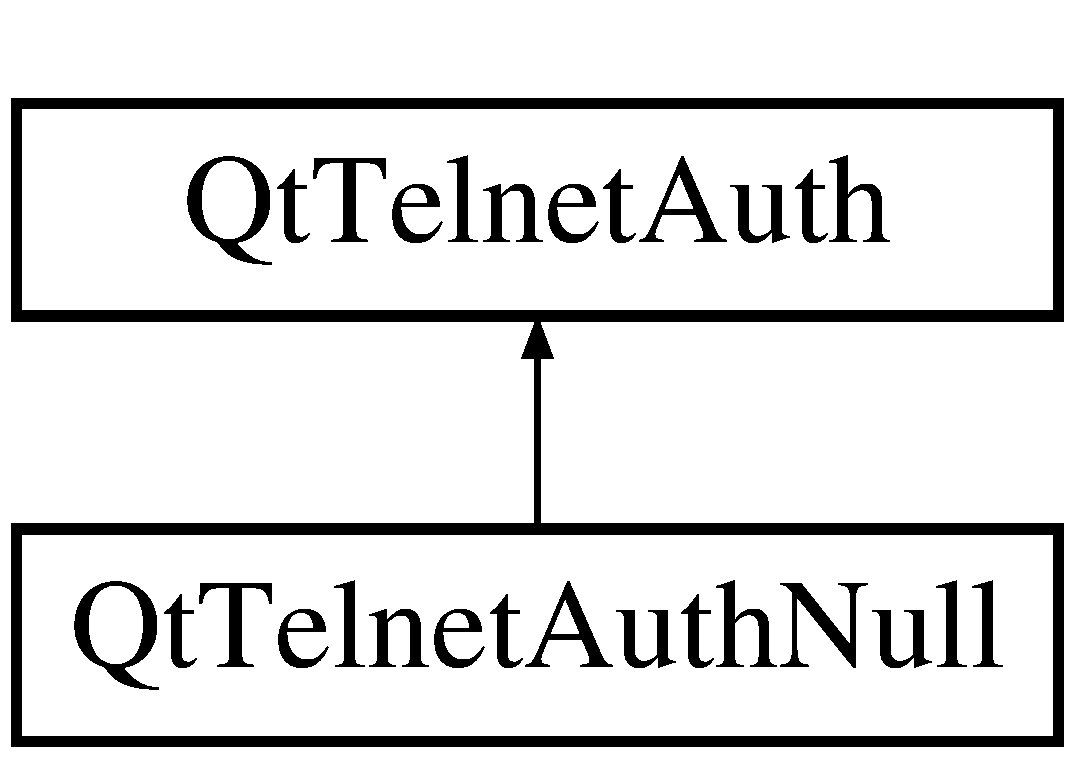
\includegraphics[height=2.000000cm]{classQtTelnetAuth}
\end{center}
\end{figure}
\subsection*{Public Types}
\begin{DoxyCompactItemize}
\item 
enum \hyperlink{classQtTelnetAuth_aef4fcfe1cf60491f566b31c7f8f8f2f2}{State} \{ \hyperlink{classQtTelnetAuth_aef4fcfe1cf60491f566b31c7f8f8f2f2ae72cd9a5978207fc7d62288158e389ef}{AuthIntermediate}, 
\hyperlink{classQtTelnetAuth_aef4fcfe1cf60491f566b31c7f8f8f2f2ae0795bd80ac1a018650ae5a13cb0720a}{AuthSuccess}, 
\hyperlink{classQtTelnetAuth_aef4fcfe1cf60491f566b31c7f8f8f2f2a31851366016c0a5fd364675c9a727def}{AuthFailure}
 \}
\end{DoxyCompactItemize}
\subsection*{Public Member Functions}
\begin{DoxyCompactItemize}
\item 
\hyperlink{classQtTelnetAuth_ae7d7ea247f07ff6c9890b9d4765a645a}{QtTelnetAuth} (char code)
\item 
virtual \hyperlink{classQtTelnetAuth_a9435d78fc604e59410dc36dc9334108d}{$\sim$QtTelnetAuth} ()
\item 
int \hyperlink{classQtTelnetAuth_a3d1b6069c3be43a9ced1906b8210e452}{code} () const 
\item 
\hyperlink{classQtTelnetAuth_aef4fcfe1cf60491f566b31c7f8f8f2f2}{State} \hyperlink{classQtTelnetAuth_a472cf022d3976da5abf78916b02ade7a}{state} () const 
\item 
void \hyperlink{classQtTelnetAuth_a89803c6612426beaaaf295528915f573}{setState} (\hyperlink{classQtTelnetAuth_aef4fcfe1cf60491f566b31c7f8f8f2f2}{State} state)
\item 
virtual QByteArray \hyperlink{classQtTelnetAuth_adceeb3a4fec9b58472d7cd7f2540e575}{authStep} (const QByteArray \&data)=0
\end{DoxyCompactItemize}
\subsection*{Private Attributes}
\begin{DoxyCompactItemize}
\item 
\hyperlink{classQtTelnetAuth_aef4fcfe1cf60491f566b31c7f8f8f2f2}{State} \hyperlink{classQtTelnetAuth_a38da91878419c68ec79384b5d75b3908}{st}
\item 
int \hyperlink{classQtTelnetAuth_a708030f5805da6a12876c6cbab24dacc}{cd}
\end{DoxyCompactItemize}


\subsection{Detailed Description}


Definition at line 95 of file qttelnet.cpp.



\subsection{Member Enumeration Documentation}
\hypertarget{classQtTelnetAuth_aef4fcfe1cf60491f566b31c7f8f8f2f2}{
\index{QtTelnetAuth@{QtTelnetAuth}!State@{State}}
\index{State@{State}!QtTelnetAuth@{QtTelnetAuth}}
\subsubsection[{State}]{\setlength{\rightskip}{0pt plus 5cm}enum {\bf QtTelnetAuth::State}}}
\label{classQtTelnetAuth_aef4fcfe1cf60491f566b31c7f8f8f2f2}
\begin{Desc}
\item[Enumerator: ]\par
\begin{description}
\index{AuthIntermediate@{AuthIntermediate}!QtTelnetAuth@{QtTelnetAuth}}\index{QtTelnetAuth@{QtTelnetAuth}!AuthIntermediate@{AuthIntermediate}}\item[{\em 
\hypertarget{classQtTelnetAuth_aef4fcfe1cf60491f566b31c7f8f8f2f2ae72cd9a5978207fc7d62288158e389ef}{
AuthIntermediate}
\label{classQtTelnetAuth_aef4fcfe1cf60491f566b31c7f8f8f2f2ae72cd9a5978207fc7d62288158e389ef}
}]\index{AuthSuccess@{AuthSuccess}!QtTelnetAuth@{QtTelnetAuth}}\index{QtTelnetAuth@{QtTelnetAuth}!AuthSuccess@{AuthSuccess}}\item[{\em 
\hypertarget{classQtTelnetAuth_aef4fcfe1cf60491f566b31c7f8f8f2f2ae0795bd80ac1a018650ae5a13cb0720a}{
AuthSuccess}
\label{classQtTelnetAuth_aef4fcfe1cf60491f566b31c7f8f8f2f2ae0795bd80ac1a018650ae5a13cb0720a}
}]\index{AuthFailure@{AuthFailure}!QtTelnetAuth@{QtTelnetAuth}}\index{QtTelnetAuth@{QtTelnetAuth}!AuthFailure@{AuthFailure}}\item[{\em 
\hypertarget{classQtTelnetAuth_aef4fcfe1cf60491f566b31c7f8f8f2f2a31851366016c0a5fd364675c9a727def}{
AuthFailure}
\label{classQtTelnetAuth_aef4fcfe1cf60491f566b31c7f8f8f2f2a31851366016c0a5fd364675c9a727def}
}]\end{description}
\end{Desc}



Definition at line 98 of file qttelnet.cpp.



\subsection{Constructor \& Destructor Documentation}
\hypertarget{classQtTelnetAuth_ae7d7ea247f07ff6c9890b9d4765a645a}{
\index{QtTelnetAuth@{QtTelnetAuth}!QtTelnetAuth@{QtTelnetAuth}}
\index{QtTelnetAuth@{QtTelnetAuth}!QtTelnetAuth@{QtTelnetAuth}}
\subsubsection[{QtTelnetAuth}]{\setlength{\rightskip}{0pt plus 5cm}QtTelnetAuth::QtTelnetAuth (
\begin{DoxyParamCaption}
\item[{char}]{code}
\end{DoxyParamCaption}
)\hspace{0.3cm}{\ttfamily  \mbox{[}inline\mbox{]}}}}
\label{classQtTelnetAuth_ae7d7ea247f07ff6c9890b9d4765a645a}


Definition at line 100 of file qttelnet.cpp.

\hypertarget{classQtTelnetAuth_a9435d78fc604e59410dc36dc9334108d}{
\index{QtTelnetAuth@{QtTelnetAuth}!$\sim$QtTelnetAuth@{$\sim$QtTelnetAuth}}
\index{$\sim$QtTelnetAuth@{$\sim$QtTelnetAuth}!QtTelnetAuth@{QtTelnetAuth}}
\subsubsection[{$\sim$QtTelnetAuth}]{\setlength{\rightskip}{0pt plus 5cm}virtual QtTelnetAuth::$\sim$QtTelnetAuth (
\begin{DoxyParamCaption}
{}
\end{DoxyParamCaption}
)\hspace{0.3cm}{\ttfamily  \mbox{[}inline, virtual\mbox{]}}}}
\label{classQtTelnetAuth_a9435d78fc604e59410dc36dc9334108d}


Definition at line 101 of file qttelnet.cpp.



\subsection{Member Function Documentation}
\hypertarget{classQtTelnetAuth_adceeb3a4fec9b58472d7cd7f2540e575}{
\index{QtTelnetAuth@{QtTelnetAuth}!authStep@{authStep}}
\index{authStep@{authStep}!QtTelnetAuth@{QtTelnetAuth}}
\subsubsection[{authStep}]{\setlength{\rightskip}{0pt plus 5cm}virtual QByteArray QtTelnetAuth::authStep (
\begin{DoxyParamCaption}
\item[{const QByteArray \&}]{data}
\end{DoxyParamCaption}
)\hspace{0.3cm}{\ttfamily  \mbox{[}pure virtual\mbox{]}}}}
\label{classQtTelnetAuth_adceeb3a4fec9b58472d7cd7f2540e575}


Implemented in \hyperlink{classQtTelnetAuthNull_a76cf474cf6860aeae906bf242ac09f95}{QtTelnetAuthNull}.

\hypertarget{classQtTelnetAuth_a3d1b6069c3be43a9ced1906b8210e452}{
\index{QtTelnetAuth@{QtTelnetAuth}!code@{code}}
\index{code@{code}!QtTelnetAuth@{QtTelnetAuth}}
\subsubsection[{code}]{\setlength{\rightskip}{0pt plus 5cm}int QtTelnetAuth::code (
\begin{DoxyParamCaption}
{}
\end{DoxyParamCaption}
) const\hspace{0.3cm}{\ttfamily  \mbox{[}inline\mbox{]}}}}
\label{classQtTelnetAuth_a3d1b6069c3be43a9ced1906b8210e452}


Definition at line 103 of file qttelnet.cpp.

\hypertarget{classQtTelnetAuth_a89803c6612426beaaaf295528915f573}{
\index{QtTelnetAuth@{QtTelnetAuth}!setState@{setState}}
\index{setState@{setState}!QtTelnetAuth@{QtTelnetAuth}}
\subsubsection[{setState}]{\setlength{\rightskip}{0pt plus 5cm}void QtTelnetAuth::setState (
\begin{DoxyParamCaption}
\item[{{\bf State}}]{state}
\end{DoxyParamCaption}
)\hspace{0.3cm}{\ttfamily  \mbox{[}inline\mbox{]}}}}
\label{classQtTelnetAuth_a89803c6612426beaaaf295528915f573}


Definition at line 105 of file qttelnet.cpp.

\hypertarget{classQtTelnetAuth_a472cf022d3976da5abf78916b02ade7a}{
\index{QtTelnetAuth@{QtTelnetAuth}!state@{state}}
\index{state@{state}!QtTelnetAuth@{QtTelnetAuth}}
\subsubsection[{state}]{\setlength{\rightskip}{0pt plus 5cm}{\bf State} QtTelnetAuth::state (
\begin{DoxyParamCaption}
{}
\end{DoxyParamCaption}
) const\hspace{0.3cm}{\ttfamily  \mbox{[}inline\mbox{]}}}}
\label{classQtTelnetAuth_a472cf022d3976da5abf78916b02ade7a}


Definition at line 104 of file qttelnet.cpp.



\subsection{Member Data Documentation}
\hypertarget{classQtTelnetAuth_a708030f5805da6a12876c6cbab24dacc}{
\index{QtTelnetAuth@{QtTelnetAuth}!cd@{cd}}
\index{cd@{cd}!QtTelnetAuth@{QtTelnetAuth}}
\subsubsection[{cd}]{\setlength{\rightskip}{0pt plus 5cm}int {\bf QtTelnetAuth::cd}\hspace{0.3cm}{\ttfamily  \mbox{[}private\mbox{]}}}}
\label{classQtTelnetAuth_a708030f5805da6a12876c6cbab24dacc}


Definition at line 111 of file qttelnet.cpp.

\hypertarget{classQtTelnetAuth_a38da91878419c68ec79384b5d75b3908}{
\index{QtTelnetAuth@{QtTelnetAuth}!st@{st}}
\index{st@{st}!QtTelnetAuth@{QtTelnetAuth}}
\subsubsection[{st}]{\setlength{\rightskip}{0pt plus 5cm}{\bf State} {\bf QtTelnetAuth::st}\hspace{0.3cm}{\ttfamily  \mbox{[}private\mbox{]}}}}
\label{classQtTelnetAuth_a38da91878419c68ec79384b5d75b3908}


Definition at line 110 of file qttelnet.cpp.



The documentation for this class was generated from the following file:\begin{DoxyCompactItemize}
\item 
/e/ms/QT/qtelnet/\hyperlink{qttelnet_8cpp}{qttelnet.cpp}\end{DoxyCompactItemize}

\hypertarget{classQtTelnetAuthNull}{
\section{QtTelnetAuthNull Class Reference}
\label{classQtTelnetAuthNull}\index{QtTelnetAuthNull@{QtTelnetAuthNull}}
}
Inheritance diagram for QtTelnetAuthNull:\begin{figure}[H]
\begin{center}
\leavevmode
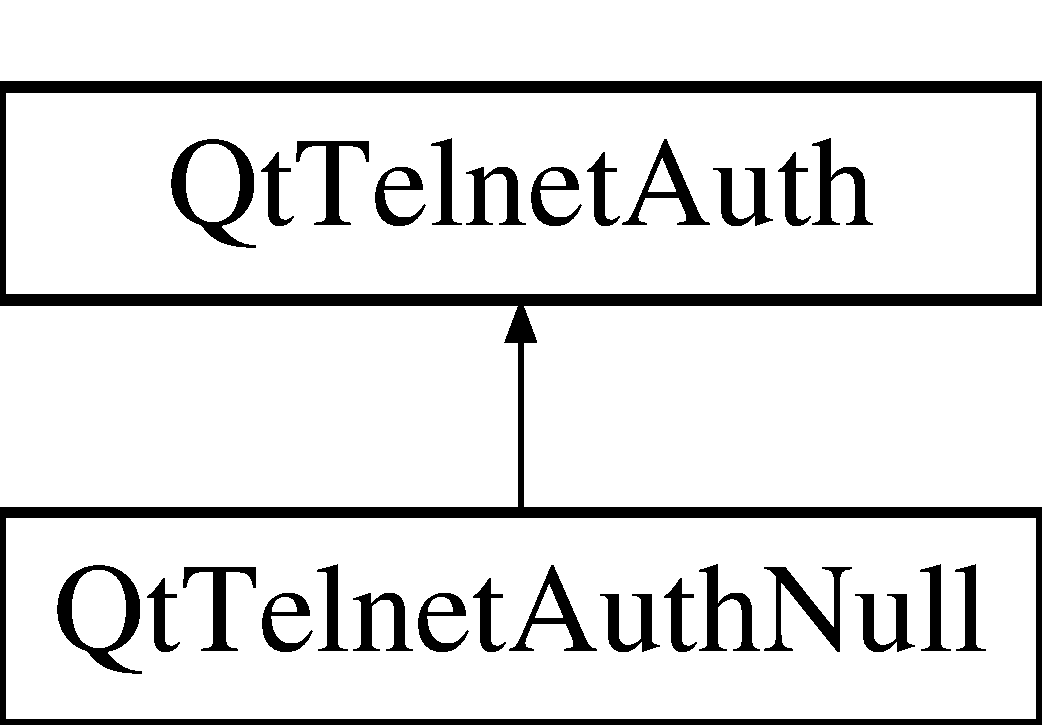
\includegraphics[height=2.000000cm]{classQtTelnetAuthNull}
\end{center}
\end{figure}
\subsection*{Public Member Functions}
\begin{DoxyCompactItemize}
\item 
\hyperlink{classQtTelnetAuthNull_a534d83b9956c696e66d3186af9ca32ef}{QtTelnetAuthNull} ()
\item 
QByteArray \hyperlink{classQtTelnetAuthNull_a76cf474cf6860aeae906bf242ac09f95}{authStep} (const QByteArray \&data)
\end{DoxyCompactItemize}


\subsection{Detailed Description}


Definition at line 473 of file qttelnet.cpp.



\subsection{Constructor \& Destructor Documentation}
\hypertarget{classQtTelnetAuthNull_a534d83b9956c696e66d3186af9ca32ef}{
\index{QtTelnetAuthNull@{QtTelnetAuthNull}!QtTelnetAuthNull@{QtTelnetAuthNull}}
\index{QtTelnetAuthNull@{QtTelnetAuthNull}!QtTelnetAuthNull@{QtTelnetAuthNull}}
\subsubsection[{QtTelnetAuthNull}]{\setlength{\rightskip}{0pt plus 5cm}QtTelnetAuthNull::QtTelnetAuthNull (
\begin{DoxyParamCaption}
{}
\end{DoxyParamCaption}
)\hspace{0.3cm}{\ttfamily  \mbox{[}inline\mbox{]}}}}
\label{classQtTelnetAuthNull_a534d83b9956c696e66d3186af9ca32ef}


Definition at line 476 of file qttelnet.cpp.



\subsection{Member Function Documentation}
\hypertarget{classQtTelnetAuthNull_a76cf474cf6860aeae906bf242ac09f95}{
\index{QtTelnetAuthNull@{QtTelnetAuthNull}!authStep@{authStep}}
\index{authStep@{authStep}!QtTelnetAuthNull@{QtTelnetAuthNull}}
\subsubsection[{authStep}]{\setlength{\rightskip}{0pt plus 5cm}QByteArray QtTelnetAuthNull::authStep (
\begin{DoxyParamCaption}
\item[{const QByteArray \&}]{data}
\end{DoxyParamCaption}
)\hspace{0.3cm}{\ttfamily  \mbox{[}virtual\mbox{]}}}}
\label{classQtTelnetAuthNull_a76cf474cf6860aeae906bf242ac09f95}


Implements \hyperlink{classQtTelnetAuth_adceeb3a4fec9b58472d7cd7f2540e575}{QtTelnetAuth}.



Definition at line 481 of file qttelnet.cpp.



The documentation for this class was generated from the following file:\begin{DoxyCompactItemize}
\item 
/e/ms/QT/qtelnet/\hyperlink{qttelnet_8cpp}{qttelnet.cpp}\end{DoxyCompactItemize}

\hypertarget{classQtTelnetPrivate}{
\section{QtTelnetPrivate Class Reference}
\label{classQtTelnetPrivate}\index{QtTelnetPrivate@{QtTelnetPrivate}}
}
\subsection*{Public Slots}
\begin{DoxyCompactItemize}
\item 
void \hyperlink{classQtTelnetPrivate_ac4be71355182f5fd94ba3470c9735f04}{socketConnected} ()
\item 
void \hyperlink{classQtTelnetPrivate_ae58ae8a85e306d69e8f0c2319784341e}{socketConnectionClosed} ()
\item 
void \hyperlink{classQtTelnetPrivate_a460c21d4294b03c64c4a63f703d474aa}{socketReadyRead} ()
\item 
void \hyperlink{classQtTelnetPrivate_ae6898112df89f6e96f465865e5d653eb}{socketError} (QAbstractSocket::SocketError error)
\item 
void \hyperlink{classQtTelnetPrivate_afc8a54ee4ba780dfa5f0a9e6019047c7}{socketException} (int)
\end{DoxyCompactItemize}
\subsection*{Public Member Functions}
\begin{DoxyCompactItemize}
\item 
\hyperlink{classQtTelnetPrivate_aec32e6a37ffe8e3463ec1dce83b88882}{QtTelnetPrivate} (\hyperlink{classQtTelnet}{QtTelnet} $\ast$parent)
\item 
\hyperlink{classQtTelnetPrivate_a64c056f9faf47ae076260359cd800c0f}{$\sim$QtTelnetPrivate} ()
\item 
bool \hyperlink{classQtTelnetPrivate_a065b1e26480f7adfba32055f11e58be3}{allowOption} (int oper, int opt)
\item 
void \hyperlink{classQtTelnetPrivate_a5ef8a8e0dac6d4f22f3b321523ce2c2b}{sendOptions} ()
\item 
void \hyperlink{classQtTelnetPrivate_a56326b558d3ceaea90abec25fa2fdf70}{sendCommand} (const QByteArray \&command)
\item 
void \hyperlink{classQtTelnetPrivate_a9fc01a0012b6c20ec64e9447fc6dc104}{sendCommand} (const char $\ast$command, int length)
\item 
void \hyperlink{classQtTelnetPrivate_abf61d8563f370b8a279b785e164a3abe}{sendCommand} (const char operation, const char option)
\item 
void \hyperlink{classQtTelnetPrivate_a1e133bd1afc78ef83c24fa02f8065ca6}{sendString} (const QString \&str)
\item 
bool \hyperlink{classQtTelnetPrivate_a507a8b94a1b244db6ca550d26ee0bd66}{replyNeeded} (uchar operation, uchar option)
\item 
void \hyperlink{classQtTelnetPrivate_aba4517cfd26c48d3cb4814c870699d95}{setMode} (uchar operation, uchar option)
\item 
bool \hyperlink{classQtTelnetPrivate_a15171a07533bd81ac5fe803b6189215d}{alreadySent} (uchar operation, uchar option)
\item 
void \hyperlink{classQtTelnetPrivate_a03a34fe9c77fe778c3a5fe74783611eb}{addSent} (uchar operation, uchar option)
\item 
void \hyperlink{classQtTelnetPrivate_aa71ecdd44e469c963cce025bd155f35b}{sendWindowSize} ()
\item 
int \hyperlink{classQtTelnetPrivate_af51d95e209673d006412d53264073573}{parsePlaintext} (const QByteArray \&data)
\item 
int \hyperlink{classQtTelnetPrivate_af6841ecc23b684b6b14065d9134795ba}{parseIAC} (const QByteArray \&data)
\item 
bool \hyperlink{classQtTelnetPrivate_adf047094261734d80497ed5e312529f3}{isOperation} (const uchar c)
\item 
bool \hyperlink{classQtTelnetPrivate_a87dc935d78d08e61c0c01742d8cafa6a}{isCommand} (const uchar c)
\item 
QByteArray \hyperlink{classQtTelnetPrivate_a50887aa4aa50718b8d8d7346becca84f}{getSubOption} (const QByteArray \&data)
\item 
void \hyperlink{classQtTelnetPrivate_a7b7516b63445c980c4159513371c6bba}{parseSubAuth} (const QByteArray \&data)
\item 
void \hyperlink{classQtTelnetPrivate_a9477255e82131a4c31f1cc643dda7298}{parseSubTT} (const QByteArray \&data)
\item 
void \hyperlink{classQtTelnetPrivate_a85ddee7ac8158da81abec0762f7b3bd3}{parseSubNAWS} (const QByteArray \&data)
\item 
uchar \hyperlink{classQtTelnetPrivate_ac3faf60570fc602551fb9b5d0afa3157}{opposite} (uchar operation, bool positive)
\item 
void \hyperlink{classQtTelnetPrivate_aaf74ce757fd90148cb60be32458d5dae}{consume} ()
\item 
void \hyperlink{classQtTelnetPrivate_a1bb6ff5139d2a05c09aad37f64042687}{setSocket} (QTcpSocket $\ast$\hyperlink{classQtTelnetPrivate_a8a3800a6c6c14c4501ac0cb5d1f9996b}{socket})
\end{DoxyCompactItemize}
\subsection*{Public Attributes}
\begin{DoxyCompactItemize}
\item 
QMap$<$ char, bool $>$ \hyperlink{classQtTelnetPrivate_a19f4f4927ab411905a637e04694dd4b4}{modes}
\item 
QList$<$ QPair$<$ uchar, uchar $>$ $>$ \hyperlink{classQtTelnetPrivate_a8c36d306aa1d9e15183f339ec9bc5862}{osent}
\item 
\hyperlink{classQtTelnet}{QtTelnet} $\ast$ \hyperlink{classQtTelnetPrivate_accc5387fdb43bf070a18bcf975134406}{q}
\item 
QTcpSocket $\ast$ \hyperlink{classQtTelnetPrivate_a8a3800a6c6c14c4501ac0cb5d1f9996b}{socket}
\item 
\hyperlink{classQtTelnetReceiveBuffer}{QtTelnetReceiveBuffer} \hyperlink{classQtTelnetPrivate_a075248a1b2a42ca268848d2d5e89040b}{buffer}
\item 
QSocketNotifier $\ast$ \hyperlink{classQtTelnetPrivate_aacc76c154d962e6275960e4c48e503c9}{notifier}
\item 
QSize \hyperlink{classQtTelnetPrivate_af249e77e92cc059087ea90f48afe7f08}{windowSize}
\item 
bool \hyperlink{classQtTelnetPrivate_a974f5ee35e078ae2b13b3ad60bbb40cc}{connected}
\item 
bool \hyperlink{classQtTelnetPrivate_a2b680b042ddaada4aeb87b549669d979}{nocheckp}
\item 
bool \hyperlink{classQtTelnetPrivate_acc2df3045ddf17a821c8fd1d5e93e006}{triedlogin}
\item 
bool \hyperlink{classQtTelnetPrivate_a9314dd43d6817a310381d8867e9ed56f}{triedpass}
\item 
bool \hyperlink{classQtTelnetPrivate_a5c08132513e77454325480668f3ced49}{firsttry}
\item 
QMap$<$ int, \hyperlink{classQtTelnetAuth}{QtTelnetAuth} $\ast$ $>$ \hyperlink{classQtTelnetPrivate_af739b55b1e603436bda658ef8c94447d}{auths}
\item 
\hyperlink{classQtTelnetAuth}{QtTelnetAuth} $\ast$ \hyperlink{classQtTelnetPrivate_a5ba83994ceb1886f9aa8751edc289c2e}{curauth}
\item 
bool \hyperlink{classQtTelnetPrivate_a0b40d5a76ef06d3a224ac4623883e4c5}{nullauth}
\item 
QRegExp \hyperlink{classQtTelnetPrivate_a9e259a89ff0c66c78f16f63ec52307f5}{loginp}
\item 
QRegExp \hyperlink{classQtTelnetPrivate_ab162800a573c3b01b264a76b5e311f4b}{passp}
\item 
QRegExp \hyperlink{classQtTelnetPrivate_a2f2b0fe1bdb6bb84d9f5db5f38af0062}{promptp}
\item 
QString \hyperlink{classQtTelnetPrivate_ae443a4bb75c5d2398e4810791902a4c3}{login}
\item 
QString \hyperlink{classQtTelnetPrivate_ae4bbc9a28524e8e55071fdd9587303bc}{pass}
\end{DoxyCompactItemize}


\subsection{Detailed Description}


Definition at line 495 of file qttelnet.cpp.



\subsection{Constructor \& Destructor Documentation}
\hypertarget{classQtTelnetPrivate_aec32e6a37ffe8e3463ec1dce83b88882}{
\index{QtTelnetPrivate@{QtTelnetPrivate}!QtTelnetPrivate@{QtTelnetPrivate}}
\index{QtTelnetPrivate@{QtTelnetPrivate}!QtTelnetPrivate@{QtTelnetPrivate}}
\subsubsection[{QtTelnetPrivate}]{\setlength{\rightskip}{0pt plus 5cm}QtTelnetPrivate::QtTelnetPrivate (
\begin{DoxyParamCaption}
\item[{{\bf QtTelnet} $\ast$}]{parent}
\end{DoxyParamCaption}
)}}
\label{classQtTelnetPrivate_aec32e6a37ffe8e3463ec1dce83b88882}


Definition at line 556 of file qttelnet.cpp.

\hypertarget{classQtTelnetPrivate_a64c056f9faf47ae076260359cd800c0f}{
\index{QtTelnetPrivate@{QtTelnetPrivate}!$\sim$QtTelnetPrivate@{$\sim$QtTelnetPrivate}}
\index{$\sim$QtTelnetPrivate@{$\sim$QtTelnetPrivate}!QtTelnetPrivate@{QtTelnetPrivate}}
\subsubsection[{$\sim$QtTelnetPrivate}]{\setlength{\rightskip}{0pt plus 5cm}QtTelnetPrivate::$\sim$QtTelnetPrivate (
\begin{DoxyParamCaption}
{}
\end{DoxyParamCaption}
)}}
\label{classQtTelnetPrivate_a64c056f9faf47ae076260359cd800c0f}


Definition at line 566 of file qttelnet.cpp.



\subsection{Member Function Documentation}
\hypertarget{classQtTelnetPrivate_a03a34fe9c77fe778c3a5fe74783611eb}{
\index{QtTelnetPrivate@{QtTelnetPrivate}!addSent@{addSent}}
\index{addSent@{addSent}!QtTelnetPrivate@{QtTelnetPrivate}}
\subsubsection[{addSent}]{\setlength{\rightskip}{0pt plus 5cm}void QtTelnetPrivate::addSent (
\begin{DoxyParamCaption}
\item[{uchar}]{operation, }
\item[{uchar}]{option}
\end{DoxyParamCaption}
)}}
\label{classQtTelnetPrivate_a03a34fe9c77fe778c3a5fe74783611eb}


Definition at line 861 of file qttelnet.cpp.

\hypertarget{classQtTelnetPrivate_a065b1e26480f7adfba32055f11e58be3}{
\index{QtTelnetPrivate@{QtTelnetPrivate}!allowOption@{allowOption}}
\index{allowOption@{allowOption}!QtTelnetPrivate@{QtTelnetPrivate}}
\subsubsection[{allowOption}]{\setlength{\rightskip}{0pt plus 5cm}bool QtTelnetPrivate::allowOption (
\begin{DoxyParamCaption}
\item[{int}]{oper, }
\item[{int}]{opt}
\end{DoxyParamCaption}
)}}
\label{classQtTelnetPrivate_a065b1e26480f7adfba32055f11e58be3}


Definition at line 911 of file qttelnet.cpp.

\hypertarget{classQtTelnetPrivate_a15171a07533bd81ac5fe803b6189215d}{
\index{QtTelnetPrivate@{QtTelnetPrivate}!alreadySent@{alreadySent}}
\index{alreadySent@{alreadySent}!QtTelnetPrivate@{QtTelnetPrivate}}
\subsubsection[{alreadySent}]{\setlength{\rightskip}{0pt plus 5cm}bool QtTelnetPrivate::alreadySent (
\begin{DoxyParamCaption}
\item[{uchar}]{operation, }
\item[{uchar}]{option}
\end{DoxyParamCaption}
)}}
\label{classQtTelnetPrivate_a15171a07533bd81ac5fe803b6189215d}


Definition at line 866 of file qttelnet.cpp.

\hypertarget{classQtTelnetPrivate_aaf74ce757fd90148cb60be32458d5dae}{
\index{QtTelnetPrivate@{QtTelnetPrivate}!consume@{consume}}
\index{consume@{consume}!QtTelnetPrivate@{QtTelnetPrivate}}
\subsubsection[{consume}]{\setlength{\rightskip}{0pt plus 5cm}void QtTelnetPrivate::consume (
\begin{DoxyParamCaption}
{}
\end{DoxyParamCaption}
)}}
\label{classQtTelnetPrivate_aaf74ce757fd90148cb60be32458d5dae}


Definition at line 608 of file qttelnet.cpp.

\hypertarget{classQtTelnetPrivate_a50887aa4aa50718b8d8d7346becca84f}{
\index{QtTelnetPrivate@{QtTelnetPrivate}!getSubOption@{getSubOption}}
\index{getSubOption@{getSubOption}!QtTelnetPrivate@{QtTelnetPrivate}}
\subsubsection[{getSubOption}]{\setlength{\rightskip}{0pt plus 5cm}QByteArray QtTelnetPrivate::getSubOption (
\begin{DoxyParamCaption}
\item[{const QByteArray \&}]{data}
\end{DoxyParamCaption}
)}}
\label{classQtTelnetPrivate_a50887aa4aa50718b8d8d7346becca84f}


Definition at line 638 of file qttelnet.cpp.

\hypertarget{classQtTelnetPrivate_a87dc935d78d08e61c0c01742d8cafa6a}{
\index{QtTelnetPrivate@{QtTelnetPrivate}!isCommand@{isCommand}}
\index{isCommand@{isCommand}!QtTelnetPrivate@{QtTelnetPrivate}}
\subsubsection[{isCommand}]{\setlength{\rightskip}{0pt plus 5cm}bool QtTelnetPrivate::isCommand (
\begin{DoxyParamCaption}
\item[{const uchar}]{c}
\end{DoxyParamCaption}
)}}
\label{classQtTelnetPrivate_a87dc935d78d08e61c0c01742d8cafa6a}


Definition at line 627 of file qttelnet.cpp.

\hypertarget{classQtTelnetPrivate_adf047094261734d80497ed5e312529f3}{
\index{QtTelnetPrivate@{QtTelnetPrivate}!isOperation@{isOperation}}
\index{isOperation@{isOperation}!QtTelnetPrivate@{QtTelnetPrivate}}
\subsubsection[{isOperation}]{\setlength{\rightskip}{0pt plus 5cm}bool QtTelnetPrivate::isOperation (
\begin{DoxyParamCaption}
\item[{const uchar}]{c}
\end{DoxyParamCaption}
)}}
\label{classQtTelnetPrivate_adf047094261734d80497ed5e312529f3}


Definition at line 632 of file qttelnet.cpp.

\hypertarget{classQtTelnetPrivate_ac3faf60570fc602551fb9b5d0afa3157}{
\index{QtTelnetPrivate@{QtTelnetPrivate}!opposite@{opposite}}
\index{opposite@{opposite}!QtTelnetPrivate@{QtTelnetPrivate}}
\subsubsection[{opposite}]{\setlength{\rightskip}{0pt plus 5cm}uchar QtTelnetPrivate::opposite (
\begin{DoxyParamCaption}
\item[{uchar}]{operation, }
\item[{bool}]{positive}
\end{DoxyParamCaption}
)}}
\label{classQtTelnetPrivate_ac3faf60570fc602551fb9b5d0afa3157}


Definition at line 595 of file qttelnet.cpp.

\hypertarget{classQtTelnetPrivate_af6841ecc23b684b6b14065d9134795ba}{
\index{QtTelnetPrivate@{QtTelnetPrivate}!parseIAC@{parseIAC}}
\index{parseIAC@{parseIAC}!QtTelnetPrivate@{QtTelnetPrivate}}
\subsubsection[{parseIAC}]{\setlength{\rightskip}{0pt plus 5cm}int QtTelnetPrivate::parseIAC (
\begin{DoxyParamCaption}
\item[{const QByteArray \&}]{data}
\end{DoxyParamCaption}
)}}
\label{classQtTelnetPrivate_af6841ecc23b684b6b14065d9134795ba}


Definition at line 716 of file qttelnet.cpp.

\hypertarget{classQtTelnetPrivate_af51d95e209673d006412d53264073573}{
\index{QtTelnetPrivate@{QtTelnetPrivate}!parsePlaintext@{parsePlaintext}}
\index{parsePlaintext@{parsePlaintext}!QtTelnetPrivate@{QtTelnetPrivate}}
\subsubsection[{parsePlaintext}]{\setlength{\rightskip}{0pt plus 5cm}int QtTelnetPrivate::parsePlaintext (
\begin{DoxyParamCaption}
\item[{const QByteArray \&}]{data}
\end{DoxyParamCaption}
)}}
\label{classQtTelnetPrivate_af51d95e209673d006412d53264073573}


Definition at line 769 of file qttelnet.cpp.

\hypertarget{classQtTelnetPrivate_a7b7516b63445c980c4159513371c6bba}{
\index{QtTelnetPrivate@{QtTelnetPrivate}!parseSubAuth@{parseSubAuth}}
\index{parseSubAuth@{parseSubAuth}!QtTelnetPrivate@{QtTelnetPrivate}}
\subsubsection[{parseSubAuth}]{\setlength{\rightskip}{0pt plus 5cm}void QtTelnetPrivate::parseSubAuth (
\begin{DoxyParamCaption}
\item[{const QByteArray \&}]{data}
\end{DoxyParamCaption}
)}}
\label{classQtTelnetPrivate_a7b7516b63445c980c4159513371c6bba}


Definition at line 673 of file qttelnet.cpp.

\hypertarget{classQtTelnetPrivate_a85ddee7ac8158da81abec0762f7b3bd3}{
\index{QtTelnetPrivate@{QtTelnetPrivate}!parseSubNAWS@{parseSubNAWS}}
\index{parseSubNAWS@{parseSubNAWS}!QtTelnetPrivate@{QtTelnetPrivate}}
\subsubsection[{parseSubNAWS}]{\setlength{\rightskip}{0pt plus 5cm}void QtTelnetPrivate::parseSubNAWS (
\begin{DoxyParamCaption}
\item[{const QByteArray \&}]{data}
\end{DoxyParamCaption}
)}}
\label{classQtTelnetPrivate_a85ddee7ac8158da81abec0762f7b3bd3}


Definition at line 653 of file qttelnet.cpp.

\hypertarget{classQtTelnetPrivate_a9477255e82131a4c31f1cc643dda7298}{
\index{QtTelnetPrivate@{QtTelnetPrivate}!parseSubTT@{parseSubTT}}
\index{parseSubTT@{parseSubTT}!QtTelnetPrivate@{QtTelnetPrivate}}
\subsubsection[{parseSubTT}]{\setlength{\rightskip}{0pt plus 5cm}void QtTelnetPrivate::parseSubTT (
\begin{DoxyParamCaption}
\item[{const QByteArray \&}]{data}
\end{DoxyParamCaption}
)}}
\label{classQtTelnetPrivate_a9477255e82131a4c31f1cc643dda7298}


Definition at line 658 of file qttelnet.cpp.

\hypertarget{classQtTelnetPrivate_a507a8b94a1b244db6ca550d26ee0bd66}{
\index{QtTelnetPrivate@{QtTelnetPrivate}!replyNeeded@{replyNeeded}}
\index{replyNeeded@{replyNeeded}!QtTelnetPrivate@{QtTelnetPrivate}}
\subsubsection[{replyNeeded}]{\setlength{\rightskip}{0pt plus 5cm}bool QtTelnetPrivate::replyNeeded (
\begin{DoxyParamCaption}
\item[{uchar}]{operation, }
\item[{uchar}]{option}
\end{DoxyParamCaption}
)}}
\label{classQtTelnetPrivate_a507a8b94a1b244db6ca550d26ee0bd66}


Definition at line 823 of file qttelnet.cpp.

\hypertarget{classQtTelnetPrivate_a9fc01a0012b6c20ec64e9447fc6dc104}{
\index{QtTelnetPrivate@{QtTelnetPrivate}!sendCommand@{sendCommand}}
\index{sendCommand@{sendCommand}!QtTelnetPrivate@{QtTelnetPrivate}}
\subsubsection[{sendCommand}]{\setlength{\rightskip}{0pt plus 5cm}void QtTelnetPrivate::sendCommand (
\begin{DoxyParamCaption}
\item[{const char $\ast$}]{command, }
\item[{int}]{length}
\end{DoxyParamCaption}
)}}
\label{classQtTelnetPrivate_a9fc01a0012b6c20ec64e9447fc6dc104}


Definition at line 905 of file qttelnet.cpp.

\hypertarget{classQtTelnetPrivate_abf61d8563f370b8a279b785e164a3abe}{
\index{QtTelnetPrivate@{QtTelnetPrivate}!sendCommand@{sendCommand}}
\index{sendCommand@{sendCommand}!QtTelnetPrivate@{QtTelnetPrivate}}
\subsubsection[{sendCommand}]{\setlength{\rightskip}{0pt plus 5cm}void QtTelnetPrivate::sendCommand (
\begin{DoxyParamCaption}
\item[{const char}]{operation, }
\item[{const char}]{option}
\end{DoxyParamCaption}
)}}
\label{classQtTelnetPrivate_abf61d8563f370b8a279b785e164a3abe}


Definition at line 899 of file qttelnet.cpp.

\hypertarget{classQtTelnetPrivate_a56326b558d3ceaea90abec25fa2fdf70}{
\index{QtTelnetPrivate@{QtTelnetPrivate}!sendCommand@{sendCommand}}
\index{sendCommand@{sendCommand}!QtTelnetPrivate@{QtTelnetPrivate}}
\subsubsection[{sendCommand}]{\setlength{\rightskip}{0pt plus 5cm}void QtTelnetPrivate::sendCommand (
\begin{DoxyParamCaption}
\item[{const QByteArray \&}]{command}
\end{DoxyParamCaption}
)}}
\label{classQtTelnetPrivate_a56326b558d3ceaea90abec25fa2fdf70}


Definition at line 884 of file qttelnet.cpp.

\hypertarget{classQtTelnetPrivate_a5ef8a8e0dac6d4f22f3b321523ce2c2b}{
\index{QtTelnetPrivate@{QtTelnetPrivate}!sendOptions@{sendOptions}}
\index{sendOptions@{sendOptions}!QtTelnetPrivate@{QtTelnetPrivate}}
\subsubsection[{sendOptions}]{\setlength{\rightskip}{0pt plus 5cm}void QtTelnetPrivate::sendOptions (
\begin{DoxyParamCaption}
{}
\end{DoxyParamCaption}
)}}
\label{classQtTelnetPrivate_a5ef8a8e0dac6d4f22f3b321523ce2c2b}


Definition at line 925 of file qttelnet.cpp.

\hypertarget{classQtTelnetPrivate_a1e133bd1afc78ef83c24fa02f8065ca6}{
\index{QtTelnetPrivate@{QtTelnetPrivate}!sendString@{sendString}}
\index{sendString@{sendString}!QtTelnetPrivate@{QtTelnetPrivate}}
\subsubsection[{sendString}]{\setlength{\rightskip}{0pt plus 5cm}void QtTelnetPrivate::sendString (
\begin{DoxyParamCaption}
\item[{const QString \&}]{str}
\end{DoxyParamCaption}
)}}
\label{classQtTelnetPrivate_a1e133bd1afc78ef83c24fa02f8065ca6}


Definition at line 876 of file qttelnet.cpp.

\hypertarget{classQtTelnetPrivate_aa71ecdd44e469c963cce025bd155f35b}{
\index{QtTelnetPrivate@{QtTelnetPrivate}!sendWindowSize@{sendWindowSize}}
\index{sendWindowSize@{sendWindowSize}!QtTelnetPrivate@{QtTelnetPrivate}}
\subsubsection[{sendWindowSize}]{\setlength{\rightskip}{0pt plus 5cm}void QtTelnetPrivate::sendWindowSize (
\begin{DoxyParamCaption}
{}
\end{DoxyParamCaption}
)}}
\label{classQtTelnetPrivate_aa71ecdd44e469c963cce025bd155f35b}


Definition at line 846 of file qttelnet.cpp.

\hypertarget{classQtTelnetPrivate_aba4517cfd26c48d3cb4814c870699d95}{
\index{QtTelnetPrivate@{QtTelnetPrivate}!setMode@{setMode}}
\index{setMode@{setMode}!QtTelnetPrivate@{QtTelnetPrivate}}
\subsubsection[{setMode}]{\setlength{\rightskip}{0pt plus 5cm}void QtTelnetPrivate::setMode (
\begin{DoxyParamCaption}
\item[{uchar}]{operation, }
\item[{uchar}]{option}
\end{DoxyParamCaption}
)}}
\label{classQtTelnetPrivate_aba4517cfd26c48d3cb4814c870699d95}


Definition at line 836 of file qttelnet.cpp.

\hypertarget{classQtTelnetPrivate_a1bb6ff5139d2a05c09aad37f64042687}{
\index{QtTelnetPrivate@{QtTelnetPrivate}!setSocket@{setSocket}}
\index{setSocket@{setSocket}!QtTelnetPrivate@{QtTelnetPrivate}}
\subsubsection[{setSocket}]{\setlength{\rightskip}{0pt plus 5cm}void QtTelnetPrivate::setSocket (
\begin{DoxyParamCaption}
\item[{QTcpSocket $\ast$}]{socket}
\end{DoxyParamCaption}
)}}
\label{classQtTelnetPrivate_a1bb6ff5139d2a05c09aad37f64042687}


Definition at line 573 of file qttelnet.cpp.

\hypertarget{classQtTelnetPrivate_ac4be71355182f5fd94ba3470c9735f04}{
\index{QtTelnetPrivate@{QtTelnetPrivate}!socketConnected@{socketConnected}}
\index{socketConnected@{socketConnected}!QtTelnetPrivate@{QtTelnetPrivate}}
\subsubsection[{socketConnected}]{\setlength{\rightskip}{0pt plus 5cm}void QtTelnetPrivate::socketConnected (
\begin{DoxyParamCaption}
{}
\end{DoxyParamCaption}
)\hspace{0.3cm}{\ttfamily  \mbox{[}slot\mbox{]}}}}
\label{classQtTelnetPrivate_ac4be71355182f5fd94ba3470c9735f04}


Definition at line 935 of file qttelnet.cpp.

\hypertarget{classQtTelnetPrivate_ae58ae8a85e306d69e8f0c2319784341e}{
\index{QtTelnetPrivate@{QtTelnetPrivate}!socketConnectionClosed@{socketConnectionClosed}}
\index{socketConnectionClosed@{socketConnectionClosed}!QtTelnetPrivate@{QtTelnetPrivate}}
\subsubsection[{socketConnectionClosed}]{\setlength{\rightskip}{0pt plus 5cm}void QtTelnetPrivate::socketConnectionClosed (
\begin{DoxyParamCaption}
{}
\end{DoxyParamCaption}
)\hspace{0.3cm}{\ttfamily  \mbox{[}slot\mbox{]}}}}
\label{classQtTelnetPrivate_ae58ae8a85e306d69e8f0c2319784341e}


Definition at line 951 of file qttelnet.cpp.

\hypertarget{classQtTelnetPrivate_ae6898112df89f6e96f465865e5d653eb}{
\index{QtTelnetPrivate@{QtTelnetPrivate}!socketError@{socketError}}
\index{socketError@{socketError}!QtTelnetPrivate@{QtTelnetPrivate}}
\subsubsection[{socketError}]{\setlength{\rightskip}{0pt plus 5cm}void QtTelnetPrivate::socketError (
\begin{DoxyParamCaption}
\item[{QAbstractSocket::SocketError}]{error}
\end{DoxyParamCaption}
)\hspace{0.3cm}{\ttfamily  \mbox{[}slot\mbox{]}}}}
\label{classQtTelnetPrivate_ae6898112df89f6e96f465865e5d653eb}


Definition at line 965 of file qttelnet.cpp.

\hypertarget{classQtTelnetPrivate_afc8a54ee4ba780dfa5f0a9e6019047c7}{
\index{QtTelnetPrivate@{QtTelnetPrivate}!socketException@{socketException}}
\index{socketException@{socketException}!QtTelnetPrivate@{QtTelnetPrivate}}
\subsubsection[{socketException}]{\setlength{\rightskip}{0pt plus 5cm}void QtTelnetPrivate::socketException (
\begin{DoxyParamCaption}
\item[{int}]{}
\end{DoxyParamCaption}
)\hspace{0.3cm}{\ttfamily  \mbox{[}slot\mbox{]}}}}
\label{classQtTelnetPrivate_afc8a54ee4ba780dfa5f0a9e6019047c7}


Definition at line 946 of file qttelnet.cpp.

\hypertarget{classQtTelnetPrivate_a460c21d4294b03c64c4a63f703d474aa}{
\index{QtTelnetPrivate@{QtTelnetPrivate}!socketReadyRead@{socketReadyRead}}
\index{socketReadyRead@{socketReadyRead}!QtTelnetPrivate@{QtTelnetPrivate}}
\subsubsection[{socketReadyRead}]{\setlength{\rightskip}{0pt plus 5cm}void QtTelnetPrivate::socketReadyRead (
\begin{DoxyParamCaption}
{}
\end{DoxyParamCaption}
)\hspace{0.3cm}{\ttfamily  \mbox{[}slot\mbox{]}}}}
\label{classQtTelnetPrivate_a460c21d4294b03c64c4a63f703d474aa}


Definition at line 959 of file qttelnet.cpp.



\subsection{Member Data Documentation}
\hypertarget{classQtTelnetPrivate_af739b55b1e603436bda658ef8c94447d}{
\index{QtTelnetPrivate@{QtTelnetPrivate}!auths@{auths}}
\index{auths@{auths}!QtTelnetPrivate@{QtTelnetPrivate}}
\subsubsection[{auths}]{\setlength{\rightskip}{0pt plus 5cm}QMap$<$int, {\bf QtTelnetAuth}$\ast$$>$ {\bf QtTelnetPrivate::auths}}}
\label{classQtTelnetPrivate_af739b55b1e603436bda658ef8c94447d}


Definition at line 515 of file qttelnet.cpp.

\hypertarget{classQtTelnetPrivate_a075248a1b2a42ca268848d2d5e89040b}{
\index{QtTelnetPrivate@{QtTelnetPrivate}!buffer@{buffer}}
\index{buffer@{buffer}!QtTelnetPrivate@{QtTelnetPrivate}}
\subsubsection[{buffer}]{\setlength{\rightskip}{0pt plus 5cm}{\bf QtTelnetReceiveBuffer} {\bf QtTelnetPrivate::buffer}}}
\label{classQtTelnetPrivate_a075248a1b2a42ca268848d2d5e89040b}


Definition at line 507 of file qttelnet.cpp.

\hypertarget{classQtTelnetPrivate_a974f5ee35e078ae2b13b3ad60bbb40cc}{
\index{QtTelnetPrivate@{QtTelnetPrivate}!connected@{connected}}
\index{connected@{connected}!QtTelnetPrivate@{QtTelnetPrivate}}
\subsubsection[{connected}]{\setlength{\rightskip}{0pt plus 5cm}bool {\bf QtTelnetPrivate::connected}}}
\label{classQtTelnetPrivate_a974f5ee35e078ae2b13b3ad60bbb40cc}


Definition at line 512 of file qttelnet.cpp.

\hypertarget{classQtTelnetPrivate_a5ba83994ceb1886f9aa8751edc289c2e}{
\index{QtTelnetPrivate@{QtTelnetPrivate}!curauth@{curauth}}
\index{curauth@{curauth}!QtTelnetPrivate@{QtTelnetPrivate}}
\subsubsection[{curauth}]{\setlength{\rightskip}{0pt plus 5cm}{\bf QtTelnetAuth}$\ast$ {\bf QtTelnetPrivate::curauth}}}
\label{classQtTelnetPrivate_a5ba83994ceb1886f9aa8751edc289c2e}


Definition at line 516 of file qttelnet.cpp.

\hypertarget{classQtTelnetPrivate_a5c08132513e77454325480668f3ced49}{
\index{QtTelnetPrivate@{QtTelnetPrivate}!firsttry@{firsttry}}
\index{firsttry@{firsttry}!QtTelnetPrivate@{QtTelnetPrivate}}
\subsubsection[{firsttry}]{\setlength{\rightskip}{0pt plus 5cm}bool {\bf QtTelnetPrivate::firsttry}}}
\label{classQtTelnetPrivate_a5c08132513e77454325480668f3ced49}


Definition at line 513 of file qttelnet.cpp.

\hypertarget{classQtTelnetPrivate_ae443a4bb75c5d2398e4810791902a4c3}{
\index{QtTelnetPrivate@{QtTelnetPrivate}!login@{login}}
\index{login@{login}!QtTelnetPrivate@{QtTelnetPrivate}}
\subsubsection[{login}]{\setlength{\rightskip}{0pt plus 5cm}QString {\bf QtTelnetPrivate::login}}}
\label{classQtTelnetPrivate_ae443a4bb75c5d2398e4810791902a4c3}


Definition at line 520 of file qttelnet.cpp.

\hypertarget{classQtTelnetPrivate_a9e259a89ff0c66c78f16f63ec52307f5}{
\index{QtTelnetPrivate@{QtTelnetPrivate}!loginp@{loginp}}
\index{loginp@{loginp}!QtTelnetPrivate@{QtTelnetPrivate}}
\subsubsection[{loginp}]{\setlength{\rightskip}{0pt plus 5cm}QRegExp {\bf QtTelnetPrivate::loginp}}}
\label{classQtTelnetPrivate_a9e259a89ff0c66c78f16f63ec52307f5}


Definition at line 519 of file qttelnet.cpp.

\hypertarget{classQtTelnetPrivate_a19f4f4927ab411905a637e04694dd4b4}{
\index{QtTelnetPrivate@{QtTelnetPrivate}!modes@{modes}}
\index{modes@{modes}!QtTelnetPrivate@{QtTelnetPrivate}}
\subsubsection[{modes}]{\setlength{\rightskip}{0pt plus 5cm}QMap$<$char, bool$>$ {\bf QtTelnetPrivate::modes}}}
\label{classQtTelnetPrivate_a19f4f4927ab411905a637e04694dd4b4}


Definition at line 502 of file qttelnet.cpp.

\hypertarget{classQtTelnetPrivate_a2b680b042ddaada4aeb87b549669d979}{
\index{QtTelnetPrivate@{QtTelnetPrivate}!nocheckp@{nocheckp}}
\index{nocheckp@{nocheckp}!QtTelnetPrivate@{QtTelnetPrivate}}
\subsubsection[{nocheckp}]{\setlength{\rightskip}{0pt plus 5cm}bool {\bf QtTelnetPrivate::nocheckp}}}
\label{classQtTelnetPrivate_a2b680b042ddaada4aeb87b549669d979}


Definition at line 512 of file qttelnet.cpp.

\hypertarget{classQtTelnetPrivate_aacc76c154d962e6275960e4c48e503c9}{
\index{QtTelnetPrivate@{QtTelnetPrivate}!notifier@{notifier}}
\index{notifier@{notifier}!QtTelnetPrivate@{QtTelnetPrivate}}
\subsubsection[{notifier}]{\setlength{\rightskip}{0pt plus 5cm}QSocketNotifier$\ast$ {\bf QtTelnetPrivate::notifier}}}
\label{classQtTelnetPrivate_aacc76c154d962e6275960e4c48e503c9}


Definition at line 508 of file qttelnet.cpp.

\hypertarget{classQtTelnetPrivate_a0b40d5a76ef06d3a224ac4623883e4c5}{
\index{QtTelnetPrivate@{QtTelnetPrivate}!nullauth@{nullauth}}
\index{nullauth@{nullauth}!QtTelnetPrivate@{QtTelnetPrivate}}
\subsubsection[{nullauth}]{\setlength{\rightskip}{0pt plus 5cm}bool {\bf QtTelnetPrivate::nullauth}}}
\label{classQtTelnetPrivate_a0b40d5a76ef06d3a224ac4623883e4c5}


Definition at line 517 of file qttelnet.cpp.

\hypertarget{classQtTelnetPrivate_a8c36d306aa1d9e15183f339ec9bc5862}{
\index{QtTelnetPrivate@{QtTelnetPrivate}!osent@{osent}}
\index{osent@{osent}!QtTelnetPrivate@{QtTelnetPrivate}}
\subsubsection[{osent}]{\setlength{\rightskip}{0pt plus 5cm}QList$<$ QPair$<$uchar, uchar$>$ $>$ {\bf QtTelnetPrivate::osent}}}
\label{classQtTelnetPrivate_a8c36d306aa1d9e15183f339ec9bc5862}


Definition at line 503 of file qttelnet.cpp.

\hypertarget{classQtTelnetPrivate_ae4bbc9a28524e8e55071fdd9587303bc}{
\index{QtTelnetPrivate@{QtTelnetPrivate}!pass@{pass}}
\index{pass@{pass}!QtTelnetPrivate@{QtTelnetPrivate}}
\subsubsection[{pass}]{\setlength{\rightskip}{0pt plus 5cm}QString {\bf QtTelnetPrivate::pass}}}
\label{classQtTelnetPrivate_ae4bbc9a28524e8e55071fdd9587303bc}


Definition at line 520 of file qttelnet.cpp.

\hypertarget{classQtTelnetPrivate_ab162800a573c3b01b264a76b5e311f4b}{
\index{QtTelnetPrivate@{QtTelnetPrivate}!passp@{passp}}
\index{passp@{passp}!QtTelnetPrivate@{QtTelnetPrivate}}
\subsubsection[{passp}]{\setlength{\rightskip}{0pt plus 5cm}QRegExp {\bf QtTelnetPrivate::passp}}}
\label{classQtTelnetPrivate_ab162800a573c3b01b264a76b5e311f4b}


Definition at line 519 of file qttelnet.cpp.

\hypertarget{classQtTelnetPrivate_a2f2b0fe1bdb6bb84d9f5db5f38af0062}{
\index{QtTelnetPrivate@{QtTelnetPrivate}!promptp@{promptp}}
\index{promptp@{promptp}!QtTelnetPrivate@{QtTelnetPrivate}}
\subsubsection[{promptp}]{\setlength{\rightskip}{0pt plus 5cm}QRegExp {\bf QtTelnetPrivate::promptp}}}
\label{classQtTelnetPrivate_a2f2b0fe1bdb6bb84d9f5db5f38af0062}


Definition at line 519 of file qttelnet.cpp.

\hypertarget{classQtTelnetPrivate_accc5387fdb43bf070a18bcf975134406}{
\index{QtTelnetPrivate@{QtTelnetPrivate}!q@{q}}
\index{q@{q}!QtTelnetPrivate@{QtTelnetPrivate}}
\subsubsection[{q}]{\setlength{\rightskip}{0pt plus 5cm}{\bf QtTelnet}$\ast$ {\bf QtTelnetPrivate::q}}}
\label{classQtTelnetPrivate_accc5387fdb43bf070a18bcf975134406}


Definition at line 505 of file qttelnet.cpp.

\hypertarget{classQtTelnetPrivate_a8a3800a6c6c14c4501ac0cb5d1f9996b}{
\index{QtTelnetPrivate@{QtTelnetPrivate}!socket@{socket}}
\index{socket@{socket}!QtTelnetPrivate@{QtTelnetPrivate}}
\subsubsection[{socket}]{\setlength{\rightskip}{0pt plus 5cm}QTcpSocket$\ast$ {\bf QtTelnetPrivate::socket}}}
\label{classQtTelnetPrivate_a8a3800a6c6c14c4501ac0cb5d1f9996b}


Definition at line 506 of file qttelnet.cpp.

\hypertarget{classQtTelnetPrivate_acc2df3045ddf17a821c8fd1d5e93e006}{
\index{QtTelnetPrivate@{QtTelnetPrivate}!triedlogin@{triedlogin}}
\index{triedlogin@{triedlogin}!QtTelnetPrivate@{QtTelnetPrivate}}
\subsubsection[{triedlogin}]{\setlength{\rightskip}{0pt plus 5cm}bool {\bf QtTelnetPrivate::triedlogin}}}
\label{classQtTelnetPrivate_acc2df3045ddf17a821c8fd1d5e93e006}


Definition at line 513 of file qttelnet.cpp.

\hypertarget{classQtTelnetPrivate_a9314dd43d6817a310381d8867e9ed56f}{
\index{QtTelnetPrivate@{QtTelnetPrivate}!triedpass@{triedpass}}
\index{triedpass@{triedpass}!QtTelnetPrivate@{QtTelnetPrivate}}
\subsubsection[{triedpass}]{\setlength{\rightskip}{0pt plus 5cm}bool {\bf QtTelnetPrivate::triedpass}}}
\label{classQtTelnetPrivate_a9314dd43d6817a310381d8867e9ed56f}


Definition at line 513 of file qttelnet.cpp.

\hypertarget{classQtTelnetPrivate_af249e77e92cc059087ea90f48afe7f08}{
\index{QtTelnetPrivate@{QtTelnetPrivate}!windowSize@{windowSize}}
\index{windowSize@{windowSize}!QtTelnetPrivate@{QtTelnetPrivate}}
\subsubsection[{windowSize}]{\setlength{\rightskip}{0pt plus 5cm}QSize {\bf QtTelnetPrivate::windowSize}}}
\label{classQtTelnetPrivate_af249e77e92cc059087ea90f48afe7f08}


Definition at line 510 of file qttelnet.cpp.



The documentation for this class was generated from the following file:\begin{DoxyCompactItemize}
\item 
/e/ms/QT/qtelnet/\hyperlink{qttelnet_8cpp}{qttelnet.cpp}\end{DoxyCompactItemize}

\hypertarget{classQtTelnetReceiveBuffer}{
\section{QtTelnetReceiveBuffer Class Reference}
\label{classQtTelnetReceiveBuffer}\index{QtTelnetReceiveBuffer@{QtTelnetReceiveBuffer}}
}
\subsection*{Public Member Functions}
\begin{DoxyCompactItemize}
\item 
\hyperlink{classQtTelnetReceiveBuffer_a3917e67c57e099710497c52b190363fc}{QtTelnetReceiveBuffer} ()
\item 
void \hyperlink{classQtTelnetReceiveBuffer_a18afe38b716bc9416699d66182fba241}{append} (const QByteArray \&data)
\item 
void \hyperlink{classQtTelnetReceiveBuffer_a24f819c851f7659918852fb0ec127093}{push\_\-back} (const QByteArray \&data)
\item 
long \hyperlink{classQtTelnetReceiveBuffer_a8d83127b574615ff6927073ef980b494}{size} () const 
\item 
QByteArray \hyperlink{classQtTelnetReceiveBuffer_a046baeae692234ac82b8e1cbd5aa630b}{readAll} ()
\end{DoxyCompactItemize}
\subsection*{Private Attributes}
\begin{DoxyCompactItemize}
\item 
QList$<$ QByteArray $>$ \hyperlink{classQtTelnetReceiveBuffer_a1b3ae3c81bfc75e232622906d19d9b3e}{buffers}
\item 
long \hyperlink{classQtTelnetReceiveBuffer_af9e8216d82fc5f1fc9a4aaff251b66bb}{bytesAvailable}
\end{DoxyCompactItemize}


\subsection{Detailed Description}


Definition at line 114 of file qttelnet.cpp.



\subsection{Constructor \& Destructor Documentation}
\hypertarget{classQtTelnetReceiveBuffer_a3917e67c57e099710497c52b190363fc}{
\index{QtTelnetReceiveBuffer@{QtTelnetReceiveBuffer}!QtTelnetReceiveBuffer@{QtTelnetReceiveBuffer}}
\index{QtTelnetReceiveBuffer@{QtTelnetReceiveBuffer}!QtTelnetReceiveBuffer@{QtTelnetReceiveBuffer}}
\subsubsection[{QtTelnetReceiveBuffer}]{\setlength{\rightskip}{0pt plus 5cm}QtTelnetReceiveBuffer::QtTelnetReceiveBuffer (
\begin{DoxyParamCaption}
{}
\end{DoxyParamCaption}
)\hspace{0.3cm}{\ttfamily  \mbox{[}inline\mbox{]}}}}
\label{classQtTelnetReceiveBuffer_a3917e67c57e099710497c52b190363fc}


Definition at line 117 of file qttelnet.cpp.



\subsection{Member Function Documentation}
\hypertarget{classQtTelnetReceiveBuffer_a18afe38b716bc9416699d66182fba241}{
\index{QtTelnetReceiveBuffer@{QtTelnetReceiveBuffer}!append@{append}}
\index{append@{append}!QtTelnetReceiveBuffer@{QtTelnetReceiveBuffer}}
\subsubsection[{append}]{\setlength{\rightskip}{0pt plus 5cm}void QtTelnetReceiveBuffer::append (
\begin{DoxyParamCaption}
\item[{const QByteArray \&}]{data}
\end{DoxyParamCaption}
)\hspace{0.3cm}{\ttfamily  \mbox{[}inline\mbox{]}}}}
\label{classQtTelnetReceiveBuffer_a18afe38b716bc9416699d66182fba241}


Definition at line 118 of file qttelnet.cpp.

\hypertarget{classQtTelnetReceiveBuffer_a24f819c851f7659918852fb0ec127093}{
\index{QtTelnetReceiveBuffer@{QtTelnetReceiveBuffer}!push\_\-back@{push\_\-back}}
\index{push\_\-back@{push\_\-back}!QtTelnetReceiveBuffer@{QtTelnetReceiveBuffer}}
\subsubsection[{push\_\-back}]{\setlength{\rightskip}{0pt plus 5cm}void QtTelnetReceiveBuffer::push\_\-back (
\begin{DoxyParamCaption}
\item[{const QByteArray \&}]{data}
\end{DoxyParamCaption}
)\hspace{0.3cm}{\ttfamily  \mbox{[}inline\mbox{]}}}}
\label{classQtTelnetReceiveBuffer_a24f819c851f7659918852fb0ec127093}


Definition at line 119 of file qttelnet.cpp.

\hypertarget{classQtTelnetReceiveBuffer_a046baeae692234ac82b8e1cbd5aa630b}{
\index{QtTelnetReceiveBuffer@{QtTelnetReceiveBuffer}!readAll@{readAll}}
\index{readAll@{readAll}!QtTelnetReceiveBuffer@{QtTelnetReceiveBuffer}}
\subsubsection[{readAll}]{\setlength{\rightskip}{0pt plus 5cm}QByteArray QtTelnetReceiveBuffer::readAll (
\begin{DoxyParamCaption}
{}
\end{DoxyParamCaption}
)\hspace{0.3cm}{\ttfamily  \mbox{[}inline\mbox{]}}}}
\label{classQtTelnetReceiveBuffer_a046baeae692234ac82b8e1cbd5aa630b}


Definition at line 121 of file qttelnet.cpp.

\hypertarget{classQtTelnetReceiveBuffer_a8d83127b574615ff6927073ef980b494}{
\index{QtTelnetReceiveBuffer@{QtTelnetReceiveBuffer}!size@{size}}
\index{size@{size}!QtTelnetReceiveBuffer@{QtTelnetReceiveBuffer}}
\subsubsection[{size}]{\setlength{\rightskip}{0pt plus 5cm}long QtTelnetReceiveBuffer::size (
\begin{DoxyParamCaption}
{}
\end{DoxyParamCaption}
) const\hspace{0.3cm}{\ttfamily  \mbox{[}inline\mbox{]}}}}
\label{classQtTelnetReceiveBuffer_a8d83127b574615ff6927073ef980b494}


Definition at line 120 of file qttelnet.cpp.



\subsection{Member Data Documentation}
\hypertarget{classQtTelnetReceiveBuffer_a1b3ae3c81bfc75e232622906d19d9b3e}{
\index{QtTelnetReceiveBuffer@{QtTelnetReceiveBuffer}!buffers@{buffers}}
\index{buffers@{buffers}!QtTelnetReceiveBuffer@{QtTelnetReceiveBuffer}}
\subsubsection[{buffers}]{\setlength{\rightskip}{0pt plus 5cm}QList$<$QByteArray$>$ {\bf QtTelnetReceiveBuffer::buffers}\hspace{0.3cm}{\ttfamily  \mbox{[}private\mbox{]}}}}
\label{classQtTelnetReceiveBuffer_a1b3ae3c81bfc75e232622906d19d9b3e}


Definition at line 131 of file qttelnet.cpp.

\hypertarget{classQtTelnetReceiveBuffer_af9e8216d82fc5f1fc9a4aaff251b66bb}{
\index{QtTelnetReceiveBuffer@{QtTelnetReceiveBuffer}!bytesAvailable@{bytesAvailable}}
\index{bytesAvailable@{bytesAvailable}!QtTelnetReceiveBuffer@{QtTelnetReceiveBuffer}}
\subsubsection[{bytesAvailable}]{\setlength{\rightskip}{0pt plus 5cm}long {\bf QtTelnetReceiveBuffer::bytesAvailable}\hspace{0.3cm}{\ttfamily  \mbox{[}private\mbox{]}}}}
\label{classQtTelnetReceiveBuffer_af9e8216d82fc5f1fc9a4aaff251b66bb}


Definition at line 132 of file qttelnet.cpp.



The documentation for this class was generated from the following file:\begin{DoxyCompactItemize}
\item 
/e/ms/QT/qtelnet/\hyperlink{qttelnet_8cpp}{qttelnet.cpp}\end{DoxyCompactItemize}

\hypertarget{classResponse}{
\section{Response Class Reference}
\label{classResponse}\index{Response@{Response}}
}


{\ttfamily \#include $<$response.h$>$}

\subsection*{Public Member Functions}
\begin{DoxyCompactItemize}
\item 
\hyperlink{classResponse_a0e0bf4f66117577315cca285dec94c20}{Response} (\hyperlink{structFgl_1_1Event}{Fgl::Event}, \hyperlink{classFglForm}{FglForm} $\ast$, bool cursorPos=false)
\end{DoxyCompactItemize}
\subsection*{Private Member Functions}
\begin{DoxyCompactItemize}
\item 
void \hyperlink{classResponse_ab76d71722c167fcf27f56403e63ab0d9}{addSyncValues} ()
\item 
void \hyperlink{classResponse_a31567b85abe887499b6b1be34975c296}{addScreenRecSyncValues} (\hyperlink{classTableView}{TableView} $\ast$)
\item 
void \hyperlink{classResponse_a94bffae67d84ecc39b939901380b2da2}{addScreenRecSyncValues} (\hyperlink{classMatrix}{Matrix} $\ast$)
\item 
void \hyperlink{classResponse_aac8433058bc5db31c052fccb7b5c32ea}{addScreenRecSyncValues} (QString)
\end{DoxyCompactItemize}
\subsection*{Private Attributes}
\begin{DoxyCompactItemize}
\item 
bool \hyperlink{classResponse_a170cc6ae7b4ad90d0c16fcdb6845415e}{showCursorPos}
\item 
\hyperlink{classFglForm}{FglForm} $\ast$ \hyperlink{classResponse_a19e3d7596e4d1a3b2af194d8e543e988}{p\_\-currForm}
\item 
QDomElement \hyperlink{classResponse_a3c59e49d41a393ac663a472135dc899a}{responseElement}
\end{DoxyCompactItemize}


\subsection{Detailed Description}


Definition at line 27 of file response.h.



\subsection{Constructor \& Destructor Documentation}
\hypertarget{classResponse_a0e0bf4f66117577315cca285dec94c20}{
\index{Response@{Response}!Response@{Response}}
\index{Response@{Response}!Response@{Response}}
\subsubsection[{Response}]{\setlength{\rightskip}{0pt plus 5cm}Response::Response (
\begin{DoxyParamCaption}
\item[{{\bf Fgl::Event}}]{id, }
\item[{{\bf FglForm} $\ast$}]{p\_\-currForm, }
\item[{bool}]{cursorPos = {\ttfamily false}}
\end{DoxyParamCaption}
)}}
\label{classResponse_a0e0bf4f66117577315cca285dec94c20}


Definition at line 25 of file response.cpp.



\subsection{Member Function Documentation}
\hypertarget{classResponse_a31567b85abe887499b6b1be34975c296}{
\index{Response@{Response}!addScreenRecSyncValues@{addScreenRecSyncValues}}
\index{addScreenRecSyncValues@{addScreenRecSyncValues}!Response@{Response}}
\subsubsection[{addScreenRecSyncValues}]{\setlength{\rightskip}{0pt plus 5cm}void Response::addScreenRecSyncValues (
\begin{DoxyParamCaption}
\item[{{\bf TableView} $\ast$}]{p\_\-screenRecord}
\end{DoxyParamCaption}
)\hspace{0.3cm}{\ttfamily  \mbox{[}private\mbox{]}}}}
\label{classResponse_a31567b85abe887499b6b1be34975c296}


Definition at line 214 of file response.cpp.

\hypertarget{classResponse_aac8433058bc5db31c052fccb7b5c32ea}{
\index{Response@{Response}!addScreenRecSyncValues@{addScreenRecSyncValues}}
\index{addScreenRecSyncValues@{addScreenRecSyncValues}!Response@{Response}}
\subsubsection[{addScreenRecSyncValues}]{\setlength{\rightskip}{0pt plus 5cm}void Response::addScreenRecSyncValues (
\begin{DoxyParamCaption}
\item[{QString}]{id}
\end{DoxyParamCaption}
)\hspace{0.3cm}{\ttfamily  \mbox{[}private\mbox{]}}}}
\label{classResponse_aac8433058bc5db31c052fccb7b5c32ea}


Definition at line 259 of file response.cpp.

\hypertarget{classResponse_a94bffae67d84ecc39b939901380b2da2}{
\index{Response@{Response}!addScreenRecSyncValues@{addScreenRecSyncValues}}
\index{addScreenRecSyncValues@{addScreenRecSyncValues}!Response@{Response}}
\subsubsection[{addScreenRecSyncValues}]{\setlength{\rightskip}{0pt plus 5cm}void Response::addScreenRecSyncValues (
\begin{DoxyParamCaption}
\item[{{\bf Matrix} $\ast$}]{}
\end{DoxyParamCaption}
)\hspace{0.3cm}{\ttfamily  \mbox{[}private\mbox{]}}}}
\label{classResponse_a94bffae67d84ecc39b939901380b2da2}
\hypertarget{classResponse_ab76d71722c167fcf27f56403e63ab0d9}{
\index{Response@{Response}!addSyncValues@{addSyncValues}}
\index{addSyncValues@{addSyncValues}!Response@{Response}}
\subsubsection[{addSyncValues}]{\setlength{\rightskip}{0pt plus 5cm}void Response::addSyncValues (
\begin{DoxyParamCaption}
{}
\end{DoxyParamCaption}
)\hspace{0.3cm}{\ttfamily  \mbox{[}private\mbox{]}}}}
\label{classResponse_ab76d71722c167fcf27f56403e63ab0d9}


Definition at line 181 of file response.cpp.



\subsection{Member Data Documentation}
\hypertarget{classResponse_a19e3d7596e4d1a3b2af194d8e543e988}{
\index{Response@{Response}!p\_\-currForm@{p\_\-currForm}}
\index{p\_\-currForm@{p\_\-currForm}!Response@{Response}}
\subsubsection[{p\_\-currForm}]{\setlength{\rightskip}{0pt plus 5cm}{\bf FglForm}$\ast$ {\bf Response::p\_\-currForm}\hspace{0.3cm}{\ttfamily  \mbox{[}private\mbox{]}}}}
\label{classResponse_a19e3d7596e4d1a3b2af194d8e543e988}


Definition at line 36 of file response.h.

\hypertarget{classResponse_a3c59e49d41a393ac663a472135dc899a}{
\index{Response@{Response}!responseElement@{responseElement}}
\index{responseElement@{responseElement}!Response@{Response}}
\subsubsection[{responseElement}]{\setlength{\rightskip}{0pt plus 5cm}QDomElement {\bf Response::responseElement}\hspace{0.3cm}{\ttfamily  \mbox{[}private\mbox{]}}}}
\label{classResponse_a3c59e49d41a393ac663a472135dc899a}


Definition at line 37 of file response.h.

\hypertarget{classResponse_a170cc6ae7b4ad90d0c16fcdb6845415e}{
\index{Response@{Response}!showCursorPos@{showCursorPos}}
\index{showCursorPos@{showCursorPos}!Response@{Response}}
\subsubsection[{showCursorPos}]{\setlength{\rightskip}{0pt plus 5cm}bool {\bf Response::showCursorPos}\hspace{0.3cm}{\ttfamily  \mbox{[}private\mbox{]}}}}
\label{classResponse_a170cc6ae7b4ad90d0c16fcdb6845415e}


Definition at line 35 of file response.h.



The documentation for this class was generated from the following files:\begin{DoxyCompactItemize}
\item 
/e/ms/QT/models/\hyperlink{response_8h}{response.h}\item 
/e/ms/QT/models/\hyperlink{response_8cpp}{response.cpp}\end{DoxyCompactItemize}

\hypertarget{classRingMenu}{
\section{RingMenu Class Reference}
\label{classRingMenu}\index{RingMenu@{RingMenu}}
}


{\ttfamily \#include $<$ringmenu.h$>$}

\subsection*{Signals}
\begin{DoxyCompactItemize}
\item 
void \hyperlink{classRingMenu_aa22f82a8f32d73a85d974f5825943d8c}{menuButtonPressed} (QString)
\end{DoxyCompactItemize}
\subsection*{Public Member Functions}
\begin{DoxyCompactItemize}
\item 
\hyperlink{classRingMenu_a161290d15ceb65ba81a049b050d73fd9}{RingMenu} (QWidget $\ast$parent=0)
\item 
\hyperlink{classRingMenu_a9315b3098d82e38ba24dab2be77ad49d}{RingMenu} (QString title, QString style=\char`\"{}\char`\"{}, QWidget $\ast$parent=0)
\item 
void \hyperlink{classRingMenu_a76fe327229667a0dda2b9b6bc4103203}{createButton} (int id=0, QString text=\char`\"{}\char`\"{}, QString desc=\char`\"{}\char`\"{})
\item 
void \hyperlink{classRingMenu_afccef718c896d4efc1085f05b4ae9737}{hideButton} (int)
\item 
void \hyperlink{classRingMenu_ac0ebc3b36ea3ae2d25e9471fac6ab271}{hideButton} (QString)
\item 
void \hyperlink{classRingMenu_a5bd5285d8e3e6de5fbcb0c96de75110c}{showButton} (QString)
\item 
void \hyperlink{classRingMenu_a8d76f877a6936c9392a91226e9f7aab9}{selectButton} (QString)
\item 
QList$<$ QPushButton $\ast$ $>$ \hyperlink{classRingMenu_ac3ba363326a56f30fd7fa7417f77a2cd}{buttons} ()
\item 
int \hyperlink{classRingMenu_adde629b6589c82f0457bf4091827878e}{buttonId} (QPushButton $\ast$button)
\item 
void \hyperlink{classRingMenu_a86e635c5a4ad42e3d8615d7f041d5a2e}{createAction} (int id=0, QString text=\char`\"{}\char`\"{})
\item 
QString \hyperlink{classRingMenu_a4255e9fe83130885f7f8d2e32d7555bf}{getMenuStyle} () const 
\item 
void \hyperlink{classRingMenu_a6a2d9d48229e85f036cf51e738092ff7}{setMenuStyle} (const QString \&ms)
\item 
QString \hyperlink{classRingMenu_a124f8251bf13042eed80479e7661ab5f}{getHideButtons} () const 
\item 
void \hyperlink{classRingMenu_a863af1bf79f57086df81812774a9d1ac}{setHideButtons} (const QString \&ms)
\item 
void \hyperlink{classRingMenu_a2daf310042d624f5bb16a21ca5833f69}{setOrientation} (const Qt::Orientation \&o)
\item 
QList$<$ QAction $\ast$ $>$ \hyperlink{classRingMenu_a051677097bff295a68a8d00d21b3cd16}{actions} ()
\item 
QAction $\ast$ \hyperlink{classRingMenu_a92c0197723e41fb50a464c4880226466}{getAction} (QString)
\item 
bool \hyperlink{classRingMenu_ac80fd9e02e31d943615f69d5e7a998aa}{isActionButton} (QPushButton $\ast$)
\item 
bool \hyperlink{classRingMenu_ab6098f804da03d7fc319d95567f09a01}{eventFilter} (QObject $\ast$obj, QEvent $\ast$event)
\end{DoxyCompactItemize}
\subsection*{Protected Member Functions}
\begin{DoxyCompactItemize}
\item 
void \hyperlink{classRingMenu_a321580d0f07f4498ef44ffc0a8d0527c}{resizeEvent} (QResizeEvent $\ast$)
\item 
void \hyperlink{classRingMenu_ab6b5988095b4d955fcdb58aed2a47320}{focusInEvent} (QFocusEvent $\ast$)
\item 
void \hyperlink{classRingMenu_a23ee1e4db5dda7e4bf83e46548ebb22a}{keyPressEvent} (QKeyEvent $\ast$)
\end{DoxyCompactItemize}
\subsection*{Properties}
\begin{DoxyCompactItemize}
\item 
QString \hyperlink{classRingMenu_af5694ea5c7af1ded9aedfbb44eaff454}{menuStyle}
\item 
QString \hyperlink{classRingMenu_ab945829d0a36844d2be8249414f587bd}{hideButtons}
\end{DoxyCompactItemize}
\subsection*{Private Types}
\begin{DoxyCompactItemize}
\item 
enum \hyperlink{classRingMenu_a549495d417ab0acc433800ec2badb3de}{ButtonHideStyle} \{ \hyperlink{classRingMenu_a549495d417ab0acc433800ec2badb3dea4874b2a8af3e7e62ee6666158882f615}{hidden}, 
\hyperlink{classRingMenu_a549495d417ab0acc433800ec2badb3dea7c0fea2b01048852bf3389e093bbd3e5}{disabled}
 \}
\end{DoxyCompactItemize}
\subsection*{Private Slots}
\begin{DoxyCompactItemize}
\item 
void \hyperlink{classRingMenu_ad28bad7db8ecd20ba7d7c5fea3151e3a}{buttonClicked} (int)
\end{DoxyCompactItemize}
\subsection*{Private Attributes}
\begin{DoxyCompactItemize}
\item 
QLayout $\ast$ \hyperlink{classRingMenu_af0f01459ece60416bad089171cfe7a2a}{layout}
\item 
QButtonGroup $\ast$ \hyperlink{classRingMenu_af6cb8d6f3b6de7197633c558020dff5d}{buttonGroup}
\item 
QString \hyperlink{classRingMenu_a44e8981a662fcf261033a1b81e8c2c17}{m\_\-menuStyle}
\item 
QString \hyperlink{classRingMenu_af9f395e6f878ed78c19507f1aea10085}{m\_\-hideButtons}
\item 
bool \hyperlink{classRingMenu_aea35804a8279e64176a639c1d16a8be1}{b\_\-hideButtons}
\item 
QList$<$ QAction $\ast$ $>$ \hyperlink{classRingMenu_a019bd2cb1e166b982396829515e7eb81}{ql\_\-menuCommands}
\item 
QList$<$ QAction $\ast$ $>$ \hyperlink{classRingMenu_a5f21339751f39c89451aab407339bbb2}{ql\_\-menuActions}
\end{DoxyCompactItemize}


\subsection{Detailed Description}


Definition at line 25 of file ringmenu.h.



\subsection{Member Enumeration Documentation}
\hypertarget{classRingMenu_a549495d417ab0acc433800ec2badb3de}{
\index{RingMenu@{RingMenu}!ButtonHideStyle@{ButtonHideStyle}}
\index{ButtonHideStyle@{ButtonHideStyle}!RingMenu@{RingMenu}}
\subsubsection[{ButtonHideStyle}]{\setlength{\rightskip}{0pt plus 5cm}enum {\bf RingMenu::ButtonHideStyle}\hspace{0.3cm}{\ttfamily  \mbox{[}private\mbox{]}}}}
\label{classRingMenu_a549495d417ab0acc433800ec2badb3de}
\begin{Desc}
\item[Enumerator: ]\par
\begin{description}
\index{hidden@{hidden}!RingMenu@{RingMenu}}\index{RingMenu@{RingMenu}!hidden@{hidden}}\item[{\em 
\hypertarget{classRingMenu_a549495d417ab0acc433800ec2badb3dea4874b2a8af3e7e62ee6666158882f615}{
hidden}
\label{classRingMenu_a549495d417ab0acc433800ec2badb3dea4874b2a8af3e7e62ee6666158882f615}
}]\index{disabled@{disabled}!RingMenu@{RingMenu}}\index{RingMenu@{RingMenu}!disabled@{disabled}}\item[{\em 
\hypertarget{classRingMenu_a549495d417ab0acc433800ec2badb3dea7c0fea2b01048852bf3389e093bbd3e5}{
disabled}
\label{classRingMenu_a549495d417ab0acc433800ec2badb3dea7c0fea2b01048852bf3389e093bbd3e5}
}]\end{description}
\end{Desc}



Definition at line 29 of file ringmenu.h.



\subsection{Constructor \& Destructor Documentation}
\hypertarget{classRingMenu_a161290d15ceb65ba81a049b050d73fd9}{
\index{RingMenu@{RingMenu}!RingMenu@{RingMenu}}
\index{RingMenu@{RingMenu}!RingMenu@{RingMenu}}
\subsubsection[{RingMenu}]{\setlength{\rightskip}{0pt plus 5cm}RingMenu::RingMenu (
\begin{DoxyParamCaption}
\item[{QWidget $\ast$}]{parent = {\ttfamily 0}}
\end{DoxyParamCaption}
)}}
\label{classRingMenu_a161290d15ceb65ba81a049b050d73fd9}


Definition at line 32 of file ringmenu.cpp.

\hypertarget{classRingMenu_a9315b3098d82e38ba24dab2be77ad49d}{
\index{RingMenu@{RingMenu}!RingMenu@{RingMenu}}
\index{RingMenu@{RingMenu}!RingMenu@{RingMenu}}
\subsubsection[{RingMenu}]{\setlength{\rightskip}{0pt plus 5cm}RingMenu::RingMenu (
\begin{DoxyParamCaption}
\item[{QString}]{title, }
\item[{QString}]{style = {\ttfamily \char`\"{}\char`\"{}}, }
\item[{QWidget $\ast$}]{parent = {\ttfamily 0}}
\end{DoxyParamCaption}
)}}
\label{classRingMenu_a9315b3098d82e38ba24dab2be77ad49d}


Definition at line 56 of file ringmenu.cpp.



\subsection{Member Function Documentation}
\hypertarget{classRingMenu_a051677097bff295a68a8d00d21b3cd16}{
\index{RingMenu@{RingMenu}!actions@{actions}}
\index{actions@{actions}!RingMenu@{RingMenu}}
\subsubsection[{actions}]{\setlength{\rightskip}{0pt plus 5cm}QList$<$ QAction $\ast$ $>$ RingMenu::actions (
\begin{DoxyParamCaption}
{}
\end{DoxyParamCaption}
)}}
\label{classRingMenu_a051677097bff295a68a8d00d21b3cd16}


Definition at line 413 of file ringmenu.cpp.

\hypertarget{classRingMenu_ad28bad7db8ecd20ba7d7c5fea3151e3a}{
\index{RingMenu@{RingMenu}!buttonClicked@{buttonClicked}}
\index{buttonClicked@{buttonClicked}!RingMenu@{RingMenu}}
\subsubsection[{buttonClicked}]{\setlength{\rightskip}{0pt plus 5cm}void RingMenu::buttonClicked (
\begin{DoxyParamCaption}
\item[{int}]{id}
\end{DoxyParamCaption}
)\hspace{0.3cm}{\ttfamily  \mbox{[}private, slot\mbox{]}}}}
\label{classRingMenu_ad28bad7db8ecd20ba7d7c5fea3151e3a}


Definition at line 277 of file ringmenu.cpp.

\hypertarget{classRingMenu_adde629b6589c82f0457bf4091827878e}{
\index{RingMenu@{RingMenu}!buttonId@{buttonId}}
\index{buttonId@{buttonId}!RingMenu@{RingMenu}}
\subsubsection[{buttonId}]{\setlength{\rightskip}{0pt plus 5cm}int RingMenu::buttonId (
\begin{DoxyParamCaption}
\item[{QPushButton $\ast$}]{button}
\end{DoxyParamCaption}
)\hspace{0.3cm}{\ttfamily  \mbox{[}inline\mbox{]}}}}
\label{classRingMenu_adde629b6589c82f0457bf4091827878e}


Definition at line 53 of file ringmenu.h.

\hypertarget{classRingMenu_ac3ba363326a56f30fd7fa7417f77a2cd}{
\index{RingMenu@{RingMenu}!buttons@{buttons}}
\index{buttons@{buttons}!RingMenu@{RingMenu}}
\subsubsection[{buttons}]{\setlength{\rightskip}{0pt plus 5cm}QList$<$ QPushButton $\ast$ $>$ RingMenu::buttons (
\begin{DoxyParamCaption}
{}
\end{DoxyParamCaption}
)}}
\label{classRingMenu_ac3ba363326a56f30fd7fa7417f77a2cd}


Definition at line 259 of file ringmenu.cpp.

\hypertarget{classRingMenu_a86e635c5a4ad42e3d8615d7f041d5a2e}{
\index{RingMenu@{RingMenu}!createAction@{createAction}}
\index{createAction@{createAction}!RingMenu@{RingMenu}}
\subsubsection[{createAction}]{\setlength{\rightskip}{0pt plus 5cm}void RingMenu::createAction (
\begin{DoxyParamCaption}
\item[{int}]{id = {\ttfamily 0}, }
\item[{QString}]{text = {\ttfamily \char`\"{}\char`\"{}}}
\end{DoxyParamCaption}
)}}
\label{classRingMenu_a86e635c5a4ad42e3d8615d7f041d5a2e}


Definition at line 290 of file ringmenu.cpp.

\hypertarget{classRingMenu_a76fe327229667a0dda2b9b6bc4103203}{
\index{RingMenu@{RingMenu}!createButton@{createButton}}
\index{createButton@{createButton}!RingMenu@{RingMenu}}
\subsubsection[{createButton}]{\setlength{\rightskip}{0pt plus 5cm}void RingMenu::createButton (
\begin{DoxyParamCaption}
\item[{int}]{id = {\ttfamily 0}, }
\item[{QString}]{text = {\ttfamily \char`\"{}\char`\"{}}, }
\item[{QString}]{desc = {\ttfamily \char`\"{}\char`\"{}}}
\end{DoxyParamCaption}
)}}
\label{classRingMenu_a76fe327229667a0dda2b9b6bc4103203}


Definition at line 97 of file ringmenu.cpp.

\hypertarget{classRingMenu_ab6098f804da03d7fc319d95567f09a01}{
\index{RingMenu@{RingMenu}!eventFilter@{eventFilter}}
\index{eventFilter@{eventFilter}!RingMenu@{RingMenu}}
\subsubsection[{eventFilter}]{\setlength{\rightskip}{0pt plus 5cm}bool RingMenu::eventFilter (
\begin{DoxyParamCaption}
\item[{QObject $\ast$}]{obj, }
\item[{QEvent $\ast$}]{event}
\end{DoxyParamCaption}
)}}
\label{classRingMenu_ab6098f804da03d7fc319d95567f09a01}


Definition at line 457 of file ringmenu.cpp.

\hypertarget{classRingMenu_ab6b5988095b4d955fcdb58aed2a47320}{
\index{RingMenu@{RingMenu}!focusInEvent@{focusInEvent}}
\index{focusInEvent@{focusInEvent}!RingMenu@{RingMenu}}
\subsubsection[{focusInEvent}]{\setlength{\rightskip}{0pt plus 5cm}void RingMenu::focusInEvent (
\begin{DoxyParamCaption}
\item[{QFocusEvent $\ast$}]{event}
\end{DoxyParamCaption}
)\hspace{0.3cm}{\ttfamily  \mbox{[}protected\mbox{]}}}}
\label{classRingMenu_ab6b5988095b4d955fcdb58aed2a47320}


Definition at line 349 of file ringmenu.cpp.

\hypertarget{classRingMenu_a92c0197723e41fb50a464c4880226466}{
\index{RingMenu@{RingMenu}!getAction@{getAction}}
\index{getAction@{getAction}!RingMenu@{RingMenu}}
\subsubsection[{getAction}]{\setlength{\rightskip}{0pt plus 5cm}QAction $\ast$ RingMenu::getAction (
\begin{DoxyParamCaption}
\item[{QString}]{name}
\end{DoxyParamCaption}
)}}
\label{classRingMenu_a92c0197723e41fb50a464c4880226466}


Definition at line 428 of file ringmenu.cpp.

\hypertarget{classRingMenu_a124f8251bf13042eed80479e7661ab5f}{
\index{RingMenu@{RingMenu}!getHideButtons@{getHideButtons}}
\index{getHideButtons@{getHideButtons}!RingMenu@{RingMenu}}
\subsubsection[{getHideButtons}]{\setlength{\rightskip}{0pt plus 5cm}QString RingMenu::getHideButtons (
\begin{DoxyParamCaption}
{}
\end{DoxyParamCaption}
) const\hspace{0.3cm}{\ttfamily  \mbox{[}inline\mbox{]}}}}
\label{classRingMenu_a124f8251bf13042eed80479e7661ab5f}


Definition at line 58 of file ringmenu.h.

\hypertarget{classRingMenu_a4255e9fe83130885f7f8d2e32d7555bf}{
\index{RingMenu@{RingMenu}!getMenuStyle@{getMenuStyle}}
\index{getMenuStyle@{getMenuStyle}!RingMenu@{RingMenu}}
\subsubsection[{getMenuStyle}]{\setlength{\rightskip}{0pt plus 5cm}QString RingMenu::getMenuStyle (
\begin{DoxyParamCaption}
{}
\end{DoxyParamCaption}
) const\hspace{0.3cm}{\ttfamily  \mbox{[}inline\mbox{]}}}}
\label{classRingMenu_a4255e9fe83130885f7f8d2e32d7555bf}


Definition at line 56 of file ringmenu.h.

\hypertarget{classRingMenu_afccef718c896d4efc1085f05b4ae9737}{
\index{RingMenu@{RingMenu}!hideButton@{hideButton}}
\index{hideButton@{hideButton}!RingMenu@{RingMenu}}
\subsubsection[{hideButton}]{\setlength{\rightskip}{0pt plus 5cm}void RingMenu::hideButton (
\begin{DoxyParamCaption}
\item[{int}]{id}
\end{DoxyParamCaption}
)}}
\label{classRingMenu_afccef718c896d4efc1085f05b4ae9737}


Definition at line 165 of file ringmenu.cpp.

\hypertarget{classRingMenu_ac0ebc3b36ea3ae2d25e9471fac6ab271}{
\index{RingMenu@{RingMenu}!hideButton@{hideButton}}
\index{hideButton@{hideButton}!RingMenu@{RingMenu}}
\subsubsection[{hideButton}]{\setlength{\rightskip}{0pt plus 5cm}void RingMenu::hideButton (
\begin{DoxyParamCaption}
\item[{QString}]{name}
\end{DoxyParamCaption}
)}}
\label{classRingMenu_ac0ebc3b36ea3ae2d25e9471fac6ab271}


Definition at line 183 of file ringmenu.cpp.

\hypertarget{classRingMenu_ac80fd9e02e31d943615f69d5e7a998aa}{
\index{RingMenu@{RingMenu}!isActionButton@{isActionButton}}
\index{isActionButton@{isActionButton}!RingMenu@{RingMenu}}
\subsubsection[{isActionButton}]{\setlength{\rightskip}{0pt plus 5cm}bool RingMenu::isActionButton (
\begin{DoxyParamCaption}
\item[{QPushButton $\ast$}]{button}
\end{DoxyParamCaption}
)}}
\label{classRingMenu_ac80fd9e02e31d943615f69d5e7a998aa}


Definition at line 449 of file ringmenu.cpp.

\hypertarget{classRingMenu_a23ee1e4db5dda7e4bf83e46548ebb22a}{
\index{RingMenu@{RingMenu}!keyPressEvent@{keyPressEvent}}
\index{keyPressEvent@{keyPressEvent}!RingMenu@{RingMenu}}
\subsubsection[{keyPressEvent}]{\setlength{\rightskip}{0pt plus 5cm}void RingMenu::keyPressEvent (
\begin{DoxyParamCaption}
\item[{QKeyEvent $\ast$}]{keyEvent}
\end{DoxyParamCaption}
)\hspace{0.3cm}{\ttfamily  \mbox{[}protected\mbox{]}}}}
\label{classRingMenu_a23ee1e4db5dda7e4bf83e46548ebb22a}


Definition at line 356 of file ringmenu.cpp.

\hypertarget{classRingMenu_aa22f82a8f32d73a85d974f5825943d8c}{
\index{RingMenu@{RingMenu}!menuButtonPressed@{menuButtonPressed}}
\index{menuButtonPressed@{menuButtonPressed}!RingMenu@{RingMenu}}
\subsubsection[{menuButtonPressed}]{\setlength{\rightskip}{0pt plus 5cm}void RingMenu::menuButtonPressed (
\begin{DoxyParamCaption}
\item[{QString}]{}
\end{DoxyParamCaption}
)\hspace{0.3cm}{\ttfamily  \mbox{[}signal\mbox{]}}}}
\label{classRingMenu_aa22f82a8f32d73a85d974f5825943d8c}
\hypertarget{classRingMenu_a321580d0f07f4498ef44ffc0a8d0527c}{
\index{RingMenu@{RingMenu}!resizeEvent@{resizeEvent}}
\index{resizeEvent@{resizeEvent}!RingMenu@{RingMenu}}
\subsubsection[{resizeEvent}]{\setlength{\rightskip}{0pt plus 5cm}void RingMenu::resizeEvent (
\begin{DoxyParamCaption}
\item[{QResizeEvent $\ast$}]{event}
\end{DoxyParamCaption}
)\hspace{0.3cm}{\ttfamily  \mbox{[}protected\mbox{]}}}}
\label{classRingMenu_a321580d0f07f4498ef44ffc0a8d0527c}


Definition at line 343 of file ringmenu.cpp.

\hypertarget{classRingMenu_a8d76f877a6936c9392a91226e9f7aab9}{
\index{RingMenu@{RingMenu}!selectButton@{selectButton}}
\index{selectButton@{selectButton}!RingMenu@{RingMenu}}
\subsubsection[{selectButton}]{\setlength{\rightskip}{0pt plus 5cm}void RingMenu::selectButton (
\begin{DoxyParamCaption}
\item[{QString}]{name}
\end{DoxyParamCaption}
)}}
\label{classRingMenu_a8d76f877a6936c9392a91226e9f7aab9}


Definition at line 238 of file ringmenu.cpp.

\hypertarget{classRingMenu_a863af1bf79f57086df81812774a9d1ac}{
\index{RingMenu@{RingMenu}!setHideButtons@{setHideButtons}}
\index{setHideButtons@{setHideButtons}!RingMenu@{RingMenu}}
\subsubsection[{setHideButtons}]{\setlength{\rightskip}{0pt plus 5cm}void RingMenu::setHideButtons (
\begin{DoxyParamCaption}
\item[{const QString \&}]{ms}
\end{DoxyParamCaption}
)}}
\label{classRingMenu_a863af1bf79f57086df81812774a9d1ac}


Definition at line 389 of file ringmenu.cpp.

\hypertarget{classRingMenu_a6a2d9d48229e85f036cf51e738092ff7}{
\index{RingMenu@{RingMenu}!setMenuStyle@{setMenuStyle}}
\index{setMenuStyle@{setMenuStyle}!RingMenu@{RingMenu}}
\subsubsection[{setMenuStyle}]{\setlength{\rightskip}{0pt plus 5cm}void RingMenu::setMenuStyle (
\begin{DoxyParamCaption}
\item[{const QString \&}]{ms}
\end{DoxyParamCaption}
)}}
\label{classRingMenu_a6a2d9d48229e85f036cf51e738092ff7}


Definition at line 381 of file ringmenu.cpp.

\hypertarget{classRingMenu_a2daf310042d624f5bb16a21ca5833f69}{
\index{RingMenu@{RingMenu}!setOrientation@{setOrientation}}
\index{setOrientation@{setOrientation}!RingMenu@{RingMenu}}
\subsubsection[{setOrientation}]{\setlength{\rightskip}{0pt plus 5cm}void RingMenu::setOrientation (
\begin{DoxyParamCaption}
\item[{const Qt::Orientation \&}]{o}
\end{DoxyParamCaption}
)}}
\label{classRingMenu_a2daf310042d624f5bb16a21ca5833f69}


Definition at line 401 of file ringmenu.cpp.

\hypertarget{classRingMenu_a5bd5285d8e3e6de5fbcb0c96de75110c}{
\index{RingMenu@{RingMenu}!showButton@{showButton}}
\index{showButton@{showButton}!RingMenu@{RingMenu}}
\subsubsection[{showButton}]{\setlength{\rightskip}{0pt plus 5cm}void RingMenu::showButton (
\begin{DoxyParamCaption}
\item[{QString}]{name}
\end{DoxyParamCaption}
)}}
\label{classRingMenu_a5bd5285d8e3e6de5fbcb0c96de75110c}


Definition at line 211 of file ringmenu.cpp.



\subsection{Member Data Documentation}
\hypertarget{classRingMenu_aea35804a8279e64176a639c1d16a8be1}{
\index{RingMenu@{RingMenu}!b\_\-hideButtons@{b\_\-hideButtons}}
\index{b\_\-hideButtons@{b\_\-hideButtons}!RingMenu@{RingMenu}}
\subsubsection[{b\_\-hideButtons}]{\setlength{\rightskip}{0pt plus 5cm}bool {\bf RingMenu::b\_\-hideButtons}\hspace{0.3cm}{\ttfamily  \mbox{[}private\mbox{]}}}}
\label{classRingMenu_aea35804a8279e64176a639c1d16a8be1}


Definition at line 72 of file ringmenu.h.

\hypertarget{classRingMenu_af6cb8d6f3b6de7197633c558020dff5d}{
\index{RingMenu@{RingMenu}!buttonGroup@{buttonGroup}}
\index{buttonGroup@{buttonGroup}!RingMenu@{RingMenu}}
\subsubsection[{buttonGroup}]{\setlength{\rightskip}{0pt plus 5cm}QButtonGroup$\ast$ {\bf RingMenu::buttonGroup}\hspace{0.3cm}{\ttfamily  \mbox{[}private\mbox{]}}}}
\label{classRingMenu_af6cb8d6f3b6de7197633c558020dff5d}


Definition at line 69 of file ringmenu.h.

\hypertarget{classRingMenu_af0f01459ece60416bad089171cfe7a2a}{
\index{RingMenu@{RingMenu}!layout@{layout}}
\index{layout@{layout}!RingMenu@{RingMenu}}
\subsubsection[{layout}]{\setlength{\rightskip}{0pt plus 5cm}QLayout$\ast$ {\bf RingMenu::layout}\hspace{0.3cm}{\ttfamily  \mbox{[}private\mbox{]}}}}
\label{classRingMenu_af0f01459ece60416bad089171cfe7a2a}


Definition at line 68 of file ringmenu.h.

\hypertarget{classRingMenu_af9f395e6f878ed78c19507f1aea10085}{
\index{RingMenu@{RingMenu}!m\_\-hideButtons@{m\_\-hideButtons}}
\index{m\_\-hideButtons@{m\_\-hideButtons}!RingMenu@{RingMenu}}
\subsubsection[{m\_\-hideButtons}]{\setlength{\rightskip}{0pt plus 5cm}QString {\bf RingMenu::m\_\-hideButtons}\hspace{0.3cm}{\ttfamily  \mbox{[}private\mbox{]}}}}
\label{classRingMenu_af9f395e6f878ed78c19507f1aea10085}


Definition at line 71 of file ringmenu.h.

\hypertarget{classRingMenu_a44e8981a662fcf261033a1b81e8c2c17}{
\index{RingMenu@{RingMenu}!m\_\-menuStyle@{m\_\-menuStyle}}
\index{m\_\-menuStyle@{m\_\-menuStyle}!RingMenu@{RingMenu}}
\subsubsection[{m\_\-menuStyle}]{\setlength{\rightskip}{0pt plus 5cm}QString {\bf RingMenu::m\_\-menuStyle}\hspace{0.3cm}{\ttfamily  \mbox{[}private\mbox{]}}}}
\label{classRingMenu_a44e8981a662fcf261033a1b81e8c2c17}


Definition at line 70 of file ringmenu.h.

\hypertarget{classRingMenu_a5f21339751f39c89451aab407339bbb2}{
\index{RingMenu@{RingMenu}!ql\_\-menuActions@{ql\_\-menuActions}}
\index{ql\_\-menuActions@{ql\_\-menuActions}!RingMenu@{RingMenu}}
\subsubsection[{ql\_\-menuActions}]{\setlength{\rightskip}{0pt plus 5cm}QList$<$QAction$\ast$$>$ {\bf RingMenu::ql\_\-menuActions}\hspace{0.3cm}{\ttfamily  \mbox{[}private\mbox{]}}}}
\label{classRingMenu_a5f21339751f39c89451aab407339bbb2}


Definition at line 74 of file ringmenu.h.

\hypertarget{classRingMenu_a019bd2cb1e166b982396829515e7eb81}{
\index{RingMenu@{RingMenu}!ql\_\-menuCommands@{ql\_\-menuCommands}}
\index{ql\_\-menuCommands@{ql\_\-menuCommands}!RingMenu@{RingMenu}}
\subsubsection[{ql\_\-menuCommands}]{\setlength{\rightskip}{0pt plus 5cm}QList$<$QAction$\ast$$>$ {\bf RingMenu::ql\_\-menuCommands}\hspace{0.3cm}{\ttfamily  \mbox{[}private\mbox{]}}}}
\label{classRingMenu_a019bd2cb1e166b982396829515e7eb81}


Definition at line 73 of file ringmenu.h.



\subsection{Property Documentation}
\hypertarget{classRingMenu_ab945829d0a36844d2be8249414f587bd}{
\index{RingMenu@{RingMenu}!hideButtons@{hideButtons}}
\index{hideButtons@{hideButtons}!RingMenu@{RingMenu}}
\subsubsection[{hideButtons}]{\setlength{\rightskip}{0pt plus 5cm}QString RingMenu::hideButtons\hspace{0.3cm}{\ttfamily  \mbox{[}read, write\mbox{]}}}}
\label{classRingMenu_ab945829d0a36844d2be8249414f587bd}


Definition at line 39 of file ringmenu.h.

\hypertarget{classRingMenu_af5694ea5c7af1ded9aedfbb44eaff454}{
\index{RingMenu@{RingMenu}!menuStyle@{menuStyle}}
\index{menuStyle@{menuStyle}!RingMenu@{RingMenu}}
\subsubsection[{menuStyle}]{\setlength{\rightskip}{0pt plus 5cm}QString RingMenu::menuStyle\hspace{0.3cm}{\ttfamily  \mbox{[}read, write\mbox{]}}}}
\label{classRingMenu_af5694ea5c7af1ded9aedfbb44eaff454}


Definition at line 34 of file ringmenu.h.



The documentation for this class was generated from the following files:\begin{DoxyCompactItemize}
\item 
/e/ms/QT/models/\hyperlink{ringmenu_8h}{ringmenu.h}\item 
/e/ms/QT/models/\hyperlink{ringmenu_8cpp}{ringmenu.cpp}\end{DoxyCompactItemize}

\hypertarget{classSlider}{
\section{Slider Class Reference}
\label{classSlider}\index{Slider@{Slider}}
}


{\ttfamily \#include $<$vwidgets.h$>$}

\subsection*{Signals}
\begin{DoxyCompactItemize}
\item 
void \hyperlink{classSlider_aaf986943e61876997b9cf675e7ad74a8}{fieldEvent} (\hyperlink{structFgl_1_1Event}{Fgl::Event})
\end{DoxyCompactItemize}
\subsection*{Public Member Functions}
\begin{DoxyCompactItemize}
\item 
\hyperlink{classSlider_acd7026578e9ac01e146b8d2e95556d87}{Slider} (QWidget $\ast$parent=0)
\item 
void \hyperlink{classSlider_a8b327f81bcf44d0a375bd8d39ce16304}{setDefaultValue} (QString def)
\item 
QString \hyperlink{classSlider_afa7ddd6b8fc0caf48ddc0c8f530cb224}{defaultValue} ()
\end{DoxyCompactItemize}
\subsection*{Public Attributes}
\begin{DoxyCompactItemize}
\item 
QString \hyperlink{classSlider_a0c9144705adc4563388fd0bf9f9cfd07}{name}
\item 
QString \hyperlink{classSlider_a7b10afcb9c8bc9d14e1cb46dcef35eb8}{colName}
\end{DoxyCompactItemize}
\subsection*{Private Attributes}
\begin{DoxyCompactItemize}
\item 
QString \hyperlink{classSlider_ab29b1fabdaa288fa1060bf1f0aa11d5a}{qs\_\-default}
\end{DoxyCompactItemize}


\subsection{Detailed Description}


Definition at line 355 of file vwidgets.h.



\subsection{Constructor \& Destructor Documentation}
\hypertarget{classSlider_acd7026578e9ac01e146b8d2e95556d87}{
\index{Slider@{Slider}!Slider@{Slider}}
\index{Slider@{Slider}!Slider@{Slider}}
\subsubsection[{Slider}]{\setlength{\rightskip}{0pt plus 5cm}Slider::Slider (
\begin{DoxyParamCaption}
\item[{QWidget $\ast$}]{parent = {\ttfamily 0}}
\end{DoxyParamCaption}
)}}
\label{classSlider_acd7026578e9ac01e146b8d2e95556d87}


\subsection{Member Function Documentation}
\hypertarget{classSlider_afa7ddd6b8fc0caf48ddc0c8f530cb224}{
\index{Slider@{Slider}!defaultValue@{defaultValue}}
\index{defaultValue@{defaultValue}!Slider@{Slider}}
\subsubsection[{defaultValue}]{\setlength{\rightskip}{0pt plus 5cm}QString Slider::defaultValue (
\begin{DoxyParamCaption}
{}
\end{DoxyParamCaption}
)\hspace{0.3cm}{\ttfamily  \mbox{[}inline\mbox{]}}}}
\label{classSlider_afa7ddd6b8fc0caf48ddc0c8f530cb224}


Definition at line 364 of file vwidgets.h.

\hypertarget{classSlider_aaf986943e61876997b9cf675e7ad74a8}{
\index{Slider@{Slider}!fieldEvent@{fieldEvent}}
\index{fieldEvent@{fieldEvent}!Slider@{Slider}}
\subsubsection[{fieldEvent}]{\setlength{\rightskip}{0pt plus 5cm}void Slider::fieldEvent (
\begin{DoxyParamCaption}
\item[{{\bf Fgl::Event}}]{}
\end{DoxyParamCaption}
)\hspace{0.3cm}{\ttfamily  \mbox{[}signal\mbox{]}}}}
\label{classSlider_aaf986943e61876997b9cf675e7ad74a8}
\hypertarget{classSlider_a8b327f81bcf44d0a375bd8d39ce16304}{
\index{Slider@{Slider}!setDefaultValue@{setDefaultValue}}
\index{setDefaultValue@{setDefaultValue}!Slider@{Slider}}
\subsubsection[{setDefaultValue}]{\setlength{\rightskip}{0pt plus 5cm}void Slider::setDefaultValue (
\begin{DoxyParamCaption}
\item[{QString}]{def}
\end{DoxyParamCaption}
)\hspace{0.3cm}{\ttfamily  \mbox{[}inline\mbox{]}}}}
\label{classSlider_a8b327f81bcf44d0a375bd8d39ce16304}


Definition at line 363 of file vwidgets.h.



\subsection{Member Data Documentation}
\hypertarget{classSlider_a7b10afcb9c8bc9d14e1cb46dcef35eb8}{
\index{Slider@{Slider}!colName@{colName}}
\index{colName@{colName}!Slider@{Slider}}
\subsubsection[{colName}]{\setlength{\rightskip}{0pt plus 5cm}QString {\bf Slider::colName}}}
\label{classSlider_a7b10afcb9c8bc9d14e1cb46dcef35eb8}


Definition at line 362 of file vwidgets.h.

\hypertarget{classSlider_a0c9144705adc4563388fd0bf9f9cfd07}{
\index{Slider@{Slider}!name@{name}}
\index{name@{name}!Slider@{Slider}}
\subsubsection[{name}]{\setlength{\rightskip}{0pt plus 5cm}QString {\bf Slider::name}}}
\label{classSlider_a0c9144705adc4563388fd0bf9f9cfd07}


Definition at line 361 of file vwidgets.h.

\hypertarget{classSlider_ab29b1fabdaa288fa1060bf1f0aa11d5a}{
\index{Slider@{Slider}!qs\_\-default@{qs\_\-default}}
\index{qs\_\-default@{qs\_\-default}!Slider@{Slider}}
\subsubsection[{qs\_\-default}]{\setlength{\rightskip}{0pt plus 5cm}QString {\bf Slider::qs\_\-default}\hspace{0.3cm}{\ttfamily  \mbox{[}private\mbox{]}}}}
\label{classSlider_ab29b1fabdaa288fa1060bf1f0aa11d5a}


Definition at line 364 of file vwidgets.h.



The documentation for this class was generated from the following file:\begin{DoxyCompactItemize}
\item 
/e/ms/QT/models/\hyperlink{vwidgets_8h}{vwidgets.h}\end{DoxyCompactItemize}

\hypertarget{classStatusBar}{
\section{StatusBar Class Reference}
\label{classStatusBar}\index{StatusBar@{StatusBar}}
}


{\ttfamily \#include $<$statusbar.h$>$}

\subsection*{Public Member Functions}
\begin{DoxyCompactItemize}
\item 
\hyperlink{classStatusBar_a4fd786b1103f4a642f5b62fffbc07716}{StatusBar} (QWidget $\ast$parent=0)
\item 
void \hyperlink{classStatusBar_a9eaac6dc5520cf2b8967988be4f00e2c}{displayComment} (QString)
\item 
void \hyperlink{classStatusBar_a765d7e2cfa11bea3156ad980a845f929}{displayMessage} (QString)
\item 
void \hyperlink{classStatusBar_a5bd7bdcfb646d9cbb522e7083cc6ae67}{displayError} (QString)
\item 
void \hyperlink{classStatusBar_ae6593a11684b2263ccc2f7c2acefa7fa}{toggleOverwriteMode} ()
\end{DoxyCompactItemize}
\subsection*{Public Attributes}
\begin{DoxyCompactItemize}
\item 
bool \hyperlink{classStatusBar_afab52abf9f79f1a7f3f0345ea2054d68}{b\_\-overwrite}
\end{DoxyCompactItemize}
\subsection*{Private Attributes}
\begin{DoxyCompactItemize}
\item 
QLabel $\ast$ \hyperlink{classStatusBar_a154eb97a6360923937dc444f68e4fdf9}{commentLabel}
\item 
QLabel $\ast$ \hyperlink{classStatusBar_a75bb9f05dd0058406ad412b0aa04d1e7}{messageLabel}
\item 
QLabel $\ast$ \hyperlink{classStatusBar_a4b649a765f9858eb5432ae641ed8ae5e}{errorLabel}
\item 
QLabel $\ast$ \hyperlink{classStatusBar_ac733bf5674b8d1fcbef6e0ba33346a7c}{writeModeLabel}
\end{DoxyCompactItemize}


\subsection{Detailed Description}


Definition at line 25 of file statusbar.h.



\subsection{Constructor \& Destructor Documentation}
\hypertarget{classStatusBar_a4fd786b1103f4a642f5b62fffbc07716}{
\index{StatusBar@{StatusBar}!StatusBar@{StatusBar}}
\index{StatusBar@{StatusBar}!StatusBar@{StatusBar}}
\subsubsection[{StatusBar}]{\setlength{\rightskip}{0pt plus 5cm}StatusBar::StatusBar (
\begin{DoxyParamCaption}
\item[{QWidget $\ast$}]{parent = {\ttfamily 0}}
\end{DoxyParamCaption}
)}}
\label{classStatusBar_a4fd786b1103f4a642f5b62fffbc07716}


Definition at line 24 of file statusbar.cpp.



\subsection{Member Function Documentation}
\hypertarget{classStatusBar_a9eaac6dc5520cf2b8967988be4f00e2c}{
\index{StatusBar@{StatusBar}!displayComment@{displayComment}}
\index{displayComment@{displayComment}!StatusBar@{StatusBar}}
\subsubsection[{displayComment}]{\setlength{\rightskip}{0pt plus 5cm}void StatusBar::displayComment (
\begin{DoxyParamCaption}
\item[{QString}]{text}
\end{DoxyParamCaption}
)}}
\label{classStatusBar_a9eaac6dc5520cf2b8967988be4f00e2c}


Definition at line 47 of file statusbar.cpp.

\hypertarget{classStatusBar_a5bd7bdcfb646d9cbb522e7083cc6ae67}{
\index{StatusBar@{StatusBar}!displayError@{displayError}}
\index{displayError@{displayError}!StatusBar@{StatusBar}}
\subsubsection[{displayError}]{\setlength{\rightskip}{0pt plus 5cm}void StatusBar::displayError (
\begin{DoxyParamCaption}
\item[{QString}]{text}
\end{DoxyParamCaption}
)}}
\label{classStatusBar_a5bd7bdcfb646d9cbb522e7083cc6ae67}


Definition at line 61 of file statusbar.cpp.

\hypertarget{classStatusBar_a765d7e2cfa11bea3156ad980a845f929}{
\index{StatusBar@{StatusBar}!displayMessage@{displayMessage}}
\index{displayMessage@{displayMessage}!StatusBar@{StatusBar}}
\subsubsection[{displayMessage}]{\setlength{\rightskip}{0pt plus 5cm}void StatusBar::displayMessage (
\begin{DoxyParamCaption}
\item[{QString}]{text}
\end{DoxyParamCaption}
)}}
\label{classStatusBar_a765d7e2cfa11bea3156ad980a845f929}


Definition at line 54 of file statusbar.cpp.

\hypertarget{classStatusBar_ae6593a11684b2263ccc2f7c2acefa7fa}{
\index{StatusBar@{StatusBar}!toggleOverwriteMode@{toggleOverwriteMode}}
\index{toggleOverwriteMode@{toggleOverwriteMode}!StatusBar@{StatusBar}}
\subsubsection[{toggleOverwriteMode}]{\setlength{\rightskip}{0pt plus 5cm}void StatusBar::toggleOverwriteMode (
\begin{DoxyParamCaption}
{}
\end{DoxyParamCaption}
)}}
\label{classStatusBar_ae6593a11684b2263ccc2f7c2acefa7fa}


Definition at line 68 of file statusbar.cpp.



\subsection{Member Data Documentation}
\hypertarget{classStatusBar_afab52abf9f79f1a7f3f0345ea2054d68}{
\index{StatusBar@{StatusBar}!b\_\-overwrite@{b\_\-overwrite}}
\index{b\_\-overwrite@{b\_\-overwrite}!StatusBar@{StatusBar}}
\subsubsection[{b\_\-overwrite}]{\setlength{\rightskip}{0pt plus 5cm}bool {\bf StatusBar::b\_\-overwrite}}}
\label{classStatusBar_afab52abf9f79f1a7f3f0345ea2054d68}


Definition at line 35 of file statusbar.h.

\hypertarget{classStatusBar_a154eb97a6360923937dc444f68e4fdf9}{
\index{StatusBar@{StatusBar}!commentLabel@{commentLabel}}
\index{commentLabel@{commentLabel}!StatusBar@{StatusBar}}
\subsubsection[{commentLabel}]{\setlength{\rightskip}{0pt plus 5cm}QLabel$\ast$ {\bf StatusBar::commentLabel}\hspace{0.3cm}{\ttfamily  \mbox{[}private\mbox{]}}}}
\label{classStatusBar_a154eb97a6360923937dc444f68e4fdf9}


Definition at line 38 of file statusbar.h.

\hypertarget{classStatusBar_a4b649a765f9858eb5432ae641ed8ae5e}{
\index{StatusBar@{StatusBar}!errorLabel@{errorLabel}}
\index{errorLabel@{errorLabel}!StatusBar@{StatusBar}}
\subsubsection[{errorLabel}]{\setlength{\rightskip}{0pt plus 5cm}QLabel$\ast$ {\bf StatusBar::errorLabel}\hspace{0.3cm}{\ttfamily  \mbox{[}private\mbox{]}}}}
\label{classStatusBar_a4b649a765f9858eb5432ae641ed8ae5e}


Definition at line 40 of file statusbar.h.

\hypertarget{classStatusBar_a75bb9f05dd0058406ad412b0aa04d1e7}{
\index{StatusBar@{StatusBar}!messageLabel@{messageLabel}}
\index{messageLabel@{messageLabel}!StatusBar@{StatusBar}}
\subsubsection[{messageLabel}]{\setlength{\rightskip}{0pt plus 5cm}QLabel$\ast$ {\bf StatusBar::messageLabel}\hspace{0.3cm}{\ttfamily  \mbox{[}private\mbox{]}}}}
\label{classStatusBar_a75bb9f05dd0058406ad412b0aa04d1e7}


Definition at line 39 of file statusbar.h.

\hypertarget{classStatusBar_ac733bf5674b8d1fcbef6e0ba33346a7c}{
\index{StatusBar@{StatusBar}!writeModeLabel@{writeModeLabel}}
\index{writeModeLabel@{writeModeLabel}!StatusBar@{StatusBar}}
\subsubsection[{writeModeLabel}]{\setlength{\rightskip}{0pt plus 5cm}QLabel$\ast$ {\bf StatusBar::writeModeLabel}\hspace{0.3cm}{\ttfamily  \mbox{[}private\mbox{]}}}}
\label{classStatusBar_ac733bf5674b8d1fcbef6e0ba33346a7c}


Definition at line 41 of file statusbar.h.



The documentation for this class was generated from the following files:\begin{DoxyCompactItemize}
\item 
/e/ms/QT/models/\hyperlink{statusbar_8h}{statusbar.h}\item 
/e/ms/QT/models/\hyperlink{statusbar_8cpp}{statusbar.cpp}\end{DoxyCompactItemize}

\hypertarget{classTableColumn}{
\section{TableColumn Class Reference}
\label{classTableColumn}\index{TableColumn@{TableColumn}}
}


{\ttfamily \#include $<$vwidgets.h$>$}

Inheritance diagram for TableColumn:\begin{figure}[H]
\begin{center}
\leavevmode
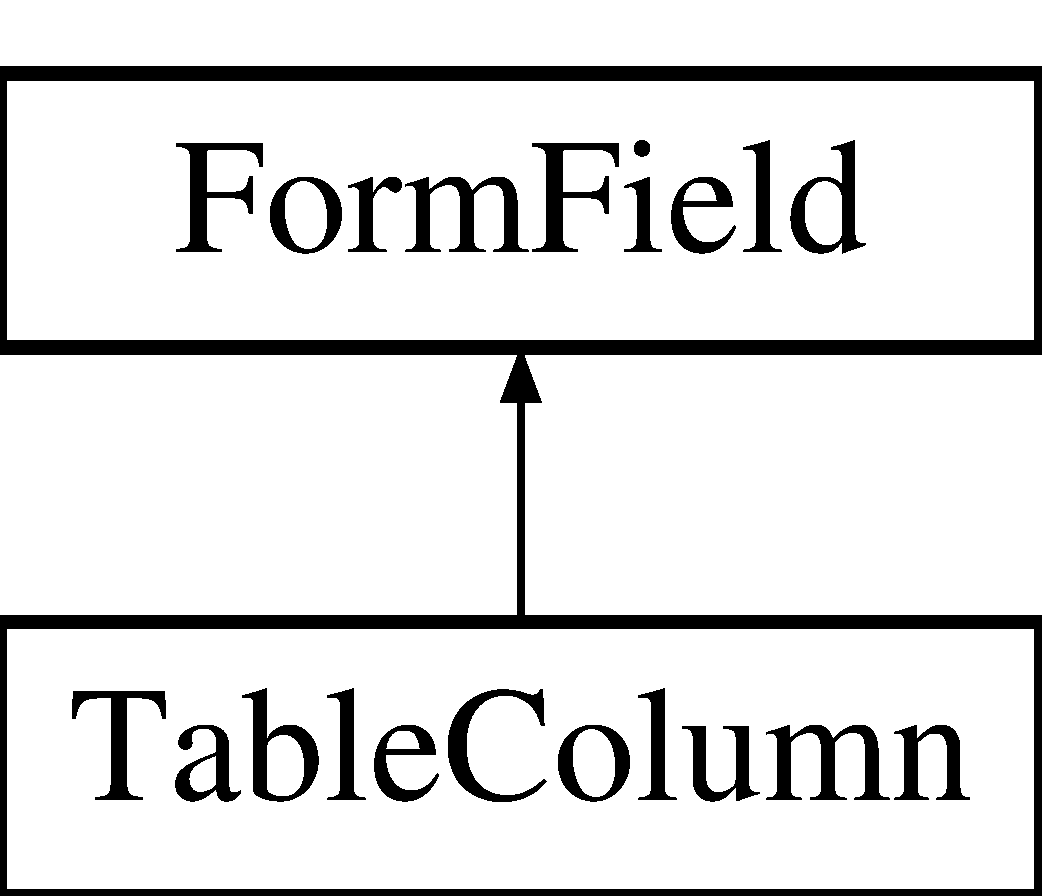
\includegraphics[height=2.000000cm]{classTableColumn}
\end{center}
\end{figure}
\subsection*{Public Member Functions}
\begin{DoxyCompactItemize}
\item 
\hyperlink{classTableColumn_addaac4b990c7df31a7055616a082ab42}{TableColumn} (QObject $\ast$parent=0)
\item 
void \hyperlink{classTableColumn_ab4e7c7bbcb467f81e8e268a2347c6b1d}{setText} (QString s=\char`\"{}\char`\"{}, int row=0)
\end{DoxyCompactItemize}


\subsection{Detailed Description}


Definition at line 104 of file vwidgets.h.



\subsection{Constructor \& Destructor Documentation}
\hypertarget{classTableColumn_addaac4b990c7df31a7055616a082ab42}{
\index{TableColumn@{TableColumn}!TableColumn@{TableColumn}}
\index{TableColumn@{TableColumn}!TableColumn@{TableColumn}}
\subsubsection[{TableColumn}]{\setlength{\rightskip}{0pt plus 5cm}TableColumn::TableColumn (
\begin{DoxyParamCaption}
\item[{QObject $\ast$}]{parent = {\ttfamily 0}}
\end{DoxyParamCaption}
)}}
\label{classTableColumn_addaac4b990c7df31a7055616a082ab42}


Definition at line 236 of file vwidgets.cpp.



\subsection{Member Function Documentation}
\hypertarget{classTableColumn_ab4e7c7bbcb467f81e8e268a2347c6b1d}{
\index{TableColumn@{TableColumn}!setText@{setText}}
\index{setText@{setText}!TableColumn@{TableColumn}}
\subsubsection[{setText}]{\setlength{\rightskip}{0pt plus 5cm}void TableColumn::setText (
\begin{DoxyParamCaption}
\item[{QString}]{s = {\ttfamily \char`\"{}\char`\"{}}, }
\item[{int}]{row = {\ttfamily 0}}
\end{DoxyParamCaption}
)}}
\label{classTableColumn_ab4e7c7bbcb467f81e8e268a2347c6b1d}


Definition at line 250 of file vwidgets.cpp.



The documentation for this class was generated from the following files:\begin{DoxyCompactItemize}
\item 
/e/ms/QT/models/\hyperlink{vwidgets_8h}{vwidgets.h}\item 
/e/ms/QT/models/\hyperlink{vwidgets_8cpp}{vwidgets.cpp}\end{DoxyCompactItemize}

\hypertarget{classTableModel}{
\section{TableModel Class Reference}
\label{classTableModel}\index{TableModel@{TableModel}}
}


{\ttfamily \#include $<$table.h$>$}

\subsection*{Public Member Functions}
\begin{DoxyCompactItemize}
\item 
\hyperlink{classTableModel_a95196d3e35846be172b6e52c2b40c099}{TableModel} (int \hyperlink{classTableModel_ab55a02518eefc1d6fc1bcf0ea62be849}{rows}, int \hyperlink{classTableModel_a363abf84b86025d76dd5f29c1e255bdd}{columns}, QObject $\ast$parent=0)
\item 
\hyperlink{classTableModel_ad7d9723995888a77fa2242069fe3e67d}{TableModel} (QObject $\ast$parent=0)
\item 
int \hyperlink{classTableModel_a053ac3f027a487a18c991bdc094a88ab}{rowCount} (const QModelIndex \&) const 
\item 
int \hyperlink{classTableModel_a3c00d361175b94462364581c57cd5871}{columnCount} (const QModelIndex \&) const 
\item 
QVariant \hyperlink{classTableModel_ab22a19802ca81ba42e1cec670e864183}{data} (const QModelIndex \&index, int role) const 
\item 
QStringList \hyperlink{classTableModel_a601afd00ae8e83cef022608eb6586a89}{mimeTypes} () const 
\item 
QMimeData $\ast$ \hyperlink{classTableModel_a8b605509eb243a62936d68373bc9a13d}{mimeData} (const QModelIndexList \&indexes) const 
\item 
bool \hyperlink{classTableModel_a6b42f2f951eb350bb7d80cffc0ebeb84}{setData} (const QModelIndex \&index, const QVariant \&value, int role)
\item 
Qt::ItemFlags \hyperlink{classTableModel_ac758b15767be92f2ac9e0c4d958d5662}{flags} (const QModelIndex \&index) const 
\item 
QVariant \hyperlink{classTableModel_a4677a49af807c3b72ca4c1e82971d9ec}{headerData} (int section, Qt::Orientation orientation, int role) const 
\item 
\hyperlink{classTableView}{TableView} $\ast$ \hyperlink{classTableModel_a220cdd35aec84f12a792899a69b615a2}{getTableView} () const 
\item 
void \hyperlink{classTableModel_a2d38aa0dc5f8d82f159adbe2c6959449}{setTableView} (\hyperlink{classTableView}{TableView} $\ast$)
\item 
int \hyperlink{classTableModel_af33093ef15d3becaa3fa0fd6b5dec732}{pageSize} () const 
\item 
int \hyperlink{classTableModel_aafaa63e6e95adc0178ce814d443dcbce}{setPageSize} (int lines)
\item 
bool \hyperlink{classTableModel_a7fcf06eebf32f5295fec05cadcdf5320}{insertRows} (int position, int \hyperlink{classTableModel_ab55a02518eefc1d6fc1bcf0ea62be849}{rows}, const QModelIndex \&index=QModelIndex())
\item 
bool \hyperlink{classTableModel_abd1d9fd2aebf4ab22a5bc1f1bc4c446d}{removeRows} (int position, int \hyperlink{classTableModel_ab55a02518eefc1d6fc1bcf0ea62be849}{rows}, const QModelIndex \&index=QModelIndex())
\end{DoxyCompactItemize}
\subsection*{Public Attributes}
\begin{DoxyCompactItemize}
\item 
QStringList \hyperlink{classTableModel_af80c02eb0f33a2c10804aae3c35699f8}{qsl\_\-colNames}
\item 
QStringList \hyperlink{classTableModel_a09bb7e46ef71f2a97ea01d73f5e2cb02}{qsl\_\-colTitleNames}
\item 
QStringList \hyperlink{classTableModel_a96ee46443dfe2b3eae27af6919781450}{qsl\_\-colTitleTabNames}
\item 
QVector$<$ QString $>$ \hyperlink{classTableModel_a8cdd6044f20e1442e77bab8f74a3d2fe}{v\_\-colTabNames}
\item 
\hyperlink{classTableView}{TableView} $\ast$ \hyperlink{classTableModel_a8971dba45716f1d616d51f9363935ace}{mytv}
\item 
bool \hyperlink{classTableModel_a575ac8236f73bfeb624eb0971e647e55}{b\_\-input}
\item 
QString \hyperlink{classTableModel_a3cf9e7d2a7d75f156247d572df42d669}{qs\_\-tabName}
\item 
QHash$<$ int, \hyperlink{classLabel}{Label} $\ast$ $>$ \hyperlink{classTableModel_a5a5e432aac68a716c4bf1849d821a846}{qh\_\-colLabels}
\item 
QStringList \hyperlink{classTableModel_ae2d3fd99f245025a7078671bb8b42225}{qsl\_\-a}
\end{DoxyCompactItemize}
\subsection*{Private Attributes}
\begin{DoxyCompactItemize}
\item 
int \hyperlink{classTableModel_a363abf84b86025d76dd5f29c1e255bdd}{columns}
\item 
int \hyperlink{classTableModel_ab55a02518eefc1d6fc1bcf0ea62be849}{rows}
\item 
int \hyperlink{classTableModel_ab9dfb638330390087383eb9373c3d419}{pagesize}
\item 
QVector$<$ QVector$<$ QString $>$ $>$ \hyperlink{classTableModel_aa7a971b1dc03dbf0392bb0c77c5a5e85}{fields}
\item 
QVector$<$ QVector$<$ QString $>$ $>$ \hyperlink{classTableModel_aaba457443a11f6e5e720ffb65b6f7191}{fields5}
\end{DoxyCompactItemize}


\subsection{Detailed Description}


Definition at line 128 of file table.h.



\subsection{Constructor \& Destructor Documentation}
\hypertarget{classTableModel_a95196d3e35846be172b6e52c2b40c099}{
\index{TableModel@{TableModel}!TableModel@{TableModel}}
\index{TableModel@{TableModel}!TableModel@{TableModel}}
\subsubsection[{TableModel}]{\setlength{\rightskip}{0pt plus 5cm}TableModel::TableModel (
\begin{DoxyParamCaption}
\item[{int}]{rows, }
\item[{int}]{columns, }
\item[{QObject $\ast$}]{parent = {\ttfamily 0}}
\end{DoxyParamCaption}
)}}
\label{classTableModel_a95196d3e35846be172b6e52c2b40c099}


Definition at line 801 of file table.cpp.

\hypertarget{classTableModel_ad7d9723995888a77fa2242069fe3e67d}{
\index{TableModel@{TableModel}!TableModel@{TableModel}}
\index{TableModel@{TableModel}!TableModel@{TableModel}}
\subsubsection[{TableModel}]{\setlength{\rightskip}{0pt plus 5cm}TableModel::TableModel (
\begin{DoxyParamCaption}
\item[{QObject $\ast$}]{parent = {\ttfamily 0}}
\end{DoxyParamCaption}
)}}
\label{classTableModel_ad7d9723995888a77fa2242069fe3e67d}


Definition at line 814 of file table.cpp.



\subsection{Member Function Documentation}
\hypertarget{classTableModel_a3c00d361175b94462364581c57cd5871}{
\index{TableModel@{TableModel}!columnCount@{columnCount}}
\index{columnCount@{columnCount}!TableModel@{TableModel}}
\subsubsection[{columnCount}]{\setlength{\rightskip}{0pt plus 5cm}int TableModel::columnCount (
\begin{DoxyParamCaption}
\item[{const QModelIndex \&}]{}
\end{DoxyParamCaption}
) const}}
\label{classTableModel_a3c00d361175b94462364581c57cd5871}


Definition at line 824 of file table.cpp.

\hypertarget{classTableModel_ab22a19802ca81ba42e1cec670e864183}{
\index{TableModel@{TableModel}!data@{data}}
\index{data@{data}!TableModel@{TableModel}}
\subsubsection[{data}]{\setlength{\rightskip}{0pt plus 5cm}QVariant TableModel::data (
\begin{DoxyParamCaption}
\item[{const QModelIndex \&}]{index, }
\item[{int}]{role}
\end{DoxyParamCaption}
) const}}
\label{classTableModel_ab22a19802ca81ba42e1cec670e864183}


Definition at line 826 of file table.cpp.

\hypertarget{classTableModel_ac758b15767be92f2ac9e0c4d958d5662}{
\index{TableModel@{TableModel}!flags@{flags}}
\index{flags@{flags}!TableModel@{TableModel}}
\subsubsection[{flags}]{\setlength{\rightskip}{0pt plus 5cm}Qt::ItemFlags TableModel::flags (
\begin{DoxyParamCaption}
\item[{const QModelIndex \&}]{index}
\end{DoxyParamCaption}
) const}}
\label{classTableModel_ac758b15767be92f2ac9e0c4d958d5662}


Definition at line 905 of file table.cpp.

\hypertarget{classTableModel_a220cdd35aec84f12a792899a69b615a2}{
\index{TableModel@{TableModel}!getTableView@{getTableView}}
\index{getTableView@{getTableView}!TableModel@{TableModel}}
\subsubsection[{getTableView}]{\setlength{\rightskip}{0pt plus 5cm}{\bf TableView}$\ast$ TableModel::getTableView (
\begin{DoxyParamCaption}
{}
\end{DoxyParamCaption}
) const\hspace{0.3cm}{\ttfamily  \mbox{[}inline\mbox{]}}}}
\label{classTableModel_a220cdd35aec84f12a792899a69b615a2}


Definition at line 152 of file table.h.

\hypertarget{classTableModel_a4677a49af807c3b72ca4c1e82971d9ec}{
\index{TableModel@{TableModel}!headerData@{headerData}}
\index{headerData@{headerData}!TableModel@{TableModel}}
\subsubsection[{headerData}]{\setlength{\rightskip}{0pt plus 5cm}QVariant TableModel::headerData (
\begin{DoxyParamCaption}
\item[{int}]{section, }
\item[{Qt::Orientation}]{orientation, }
\item[{int}]{role}
\end{DoxyParamCaption}
) const}}
\label{classTableModel_a4677a49af807c3b72ca4c1e82971d9ec}


Definition at line 1004 of file table.cpp.

\hypertarget{classTableModel_a7fcf06eebf32f5295fec05cadcdf5320}{
\index{TableModel@{TableModel}!insertRows@{insertRows}}
\index{insertRows@{insertRows}!TableModel@{TableModel}}
\subsubsection[{insertRows}]{\setlength{\rightskip}{0pt plus 5cm}bool TableModel::insertRows (
\begin{DoxyParamCaption}
\item[{int}]{position, }
\item[{int}]{rows, }
\item[{const QModelIndex \&}]{index = {\ttfamily QModelIndex()}}
\end{DoxyParamCaption}
)}}
\label{classTableModel_a7fcf06eebf32f5295fec05cadcdf5320}


Definition at line 953 of file table.cpp.

\hypertarget{classTableModel_a8b605509eb243a62936d68373bc9a13d}{
\index{TableModel@{TableModel}!mimeData@{mimeData}}
\index{mimeData@{mimeData}!TableModel@{TableModel}}
\subsubsection[{mimeData}]{\setlength{\rightskip}{0pt plus 5cm}QMimeData $\ast$ TableModel::mimeData (
\begin{DoxyParamCaption}
\item[{const QModelIndexList \&}]{indexes}
\end{DoxyParamCaption}
) const}}
\label{classTableModel_a8b605509eb243a62936d68373bc9a13d}


Definition at line 930 of file table.cpp.

\hypertarget{classTableModel_a601afd00ae8e83cef022608eb6586a89}{
\index{TableModel@{TableModel}!mimeTypes@{mimeTypes}}
\index{mimeTypes@{mimeTypes}!TableModel@{TableModel}}
\subsubsection[{mimeTypes}]{\setlength{\rightskip}{0pt plus 5cm}QStringList TableModel::mimeTypes (
\begin{DoxyParamCaption}
{}
\end{DoxyParamCaption}
) const}}
\label{classTableModel_a601afd00ae8e83cef022608eb6586a89}


Definition at line 923 of file table.cpp.

\hypertarget{classTableModel_af33093ef15d3becaa3fa0fd6b5dec732}{
\index{TableModel@{TableModel}!pageSize@{pageSize}}
\index{pageSize@{pageSize}!TableModel@{TableModel}}
\subsubsection[{pageSize}]{\setlength{\rightskip}{0pt plus 5cm}int TableModel::pageSize (
\begin{DoxyParamCaption}
{}
\end{DoxyParamCaption}
) const\hspace{0.3cm}{\ttfamily  \mbox{[}inline\mbox{]}}}}
\label{classTableModel_af33093ef15d3becaa3fa0fd6b5dec732}


Definition at line 155 of file table.h.

\hypertarget{classTableModel_abd1d9fd2aebf4ab22a5bc1f1bc4c446d}{
\index{TableModel@{TableModel}!removeRows@{removeRows}}
\index{removeRows@{removeRows}!TableModel@{TableModel}}
\subsubsection[{removeRows}]{\setlength{\rightskip}{0pt plus 5cm}bool TableModel::removeRows (
\begin{DoxyParamCaption}
\item[{int}]{position, }
\item[{int}]{rows, }
\item[{const QModelIndex \&}]{index = {\ttfamily QModelIndex()}}
\end{DoxyParamCaption}
)}}
\label{classTableModel_abd1d9fd2aebf4ab22a5bc1f1bc4c446d}


Definition at line 978 of file table.cpp.

\hypertarget{classTableModel_a053ac3f027a487a18c991bdc094a88ab}{
\index{TableModel@{TableModel}!rowCount@{rowCount}}
\index{rowCount@{rowCount}!TableModel@{TableModel}}
\subsubsection[{rowCount}]{\setlength{\rightskip}{0pt plus 5cm}int TableModel::rowCount (
\begin{DoxyParamCaption}
\item[{const QModelIndex \&}]{}
\end{DoxyParamCaption}
) const}}
\label{classTableModel_a053ac3f027a487a18c991bdc094a88ab}


Definition at line 822 of file table.cpp.

\hypertarget{classTableModel_a6b42f2f951eb350bb7d80cffc0ebeb84}{
\index{TableModel@{TableModel}!setData@{setData}}
\index{setData@{setData}!TableModel@{TableModel}}
\subsubsection[{setData}]{\setlength{\rightskip}{0pt plus 5cm}bool TableModel::setData (
\begin{DoxyParamCaption}
\item[{const QModelIndex \&}]{index, }
\item[{const QVariant \&}]{value, }
\item[{int}]{role}
\end{DoxyParamCaption}
)}}
\label{classTableModel_a6b42f2f951eb350bb7d80cffc0ebeb84}


Definition at line 889 of file table.cpp.

\hypertarget{classTableModel_aafaa63e6e95adc0178ce814d443dcbce}{
\index{TableModel@{TableModel}!setPageSize@{setPageSize}}
\index{setPageSize@{setPageSize}!TableModel@{TableModel}}
\subsubsection[{setPageSize}]{\setlength{\rightskip}{0pt plus 5cm}int TableModel::setPageSize (
\begin{DoxyParamCaption}
\item[{int}]{lines}
\end{DoxyParamCaption}
)\hspace{0.3cm}{\ttfamily  \mbox{[}inline\mbox{]}}}}
\label{classTableModel_aafaa63e6e95adc0178ce814d443dcbce}


Definition at line 156 of file table.h.

\hypertarget{classTableModel_a2d38aa0dc5f8d82f159adbe2c6959449}{
\index{TableModel@{TableModel}!setTableView@{setTableView}}
\index{setTableView@{setTableView}!TableModel@{TableModel}}
\subsubsection[{setTableView}]{\setlength{\rightskip}{0pt plus 5cm}void TableModel::setTableView (
\begin{DoxyParamCaption}
\item[{{\bf TableView} $\ast$}]{tv}
\end{DoxyParamCaption}
)}}
\label{classTableModel_a2d38aa0dc5f8d82f159adbe2c6959449}


Definition at line 999 of file table.cpp.



\subsection{Member Data Documentation}
\hypertarget{classTableModel_a575ac8236f73bfeb624eb0971e647e55}{
\index{TableModel@{TableModel}!b\_\-input@{b\_\-input}}
\index{b\_\-input@{b\_\-input}!TableModel@{TableModel}}
\subsubsection[{b\_\-input}]{\setlength{\rightskip}{0pt plus 5cm}bool {\bf TableModel::b\_\-input}}}
\label{classTableModel_a575ac8236f73bfeb624eb0971e647e55}


Definition at line 164 of file table.h.

\hypertarget{classTableModel_a363abf84b86025d76dd5f29c1e255bdd}{
\index{TableModel@{TableModel}!columns@{columns}}
\index{columns@{columns}!TableModel@{TableModel}}
\subsubsection[{columns}]{\setlength{\rightskip}{0pt plus 5cm}int {\bf TableModel::columns}\hspace{0.3cm}{\ttfamily  \mbox{[}private\mbox{]}}}}
\label{classTableModel_a363abf84b86025d76dd5f29c1e255bdd}


Definition at line 170 of file table.h.

\hypertarget{classTableModel_aa7a971b1dc03dbf0392bb0c77c5a5e85}{
\index{TableModel@{TableModel}!fields@{fields}}
\index{fields@{fields}!TableModel@{TableModel}}
\subsubsection[{fields}]{\setlength{\rightskip}{0pt plus 5cm}QVector$<$ QVector$<$QString$>$ $>$ {\bf TableModel::fields}\hspace{0.3cm}{\ttfamily  \mbox{[}private\mbox{]}}}}
\label{classTableModel_aa7a971b1dc03dbf0392bb0c77c5a5e85}


Definition at line 176 of file table.h.

\hypertarget{classTableModel_aaba457443a11f6e5e720ffb65b6f7191}{
\index{TableModel@{TableModel}!fields5@{fields5}}
\index{fields5@{fields5}!TableModel@{TableModel}}
\subsubsection[{fields5}]{\setlength{\rightskip}{0pt plus 5cm}QVector$<$ QVector$<$QString$>$ $>$ {\bf TableModel::fields5}\hspace{0.3cm}{\ttfamily  \mbox{[}private\mbox{]}}}}
\label{classTableModel_aaba457443a11f6e5e720ffb65b6f7191}


Definition at line 177 of file table.h.

\hypertarget{classTableModel_a8971dba45716f1d616d51f9363935ace}{
\index{TableModel@{TableModel}!mytv@{mytv}}
\index{mytv@{mytv}!TableModel@{TableModel}}
\subsubsection[{mytv}]{\setlength{\rightskip}{0pt plus 5cm}{\bf TableView}$\ast$ {\bf TableModel::mytv}}}
\label{classTableModel_a8971dba45716f1d616d51f9363935ace}


Definition at line 162 of file table.h.

\hypertarget{classTableModel_ab9dfb638330390087383eb9373c3d419}{
\index{TableModel@{TableModel}!pagesize@{pagesize}}
\index{pagesize@{pagesize}!TableModel@{TableModel}}
\subsubsection[{pagesize}]{\setlength{\rightskip}{0pt plus 5cm}int {\bf TableModel::pagesize}\hspace{0.3cm}{\ttfamily  \mbox{[}private\mbox{]}}}}
\label{classTableModel_ab9dfb638330390087383eb9373c3d419}


Definition at line 173 of file table.h.

\hypertarget{classTableModel_a5a5e432aac68a716c4bf1849d821a846}{
\index{TableModel@{TableModel}!qh\_\-colLabels@{qh\_\-colLabels}}
\index{qh\_\-colLabels@{qh\_\-colLabels}!TableModel@{TableModel}}
\subsubsection[{qh\_\-colLabels}]{\setlength{\rightskip}{0pt plus 5cm}QHash$<$int, {\bf Label}$\ast$$>$ {\bf TableModel::qh\_\-colLabels}}}
\label{classTableModel_a5a5e432aac68a716c4bf1849d821a846}


Definition at line 166 of file table.h.

\hypertarget{classTableModel_a3cf9e7d2a7d75f156247d572df42d669}{
\index{TableModel@{TableModel}!qs\_\-tabName@{qs\_\-tabName}}
\index{qs\_\-tabName@{qs\_\-tabName}!TableModel@{TableModel}}
\subsubsection[{qs\_\-tabName}]{\setlength{\rightskip}{0pt plus 5cm}QString {\bf TableModel::qs\_\-tabName}}}
\label{classTableModel_a3cf9e7d2a7d75f156247d572df42d669}


Definition at line 165 of file table.h.

\hypertarget{classTableModel_ae2d3fd99f245025a7078671bb8b42225}{
\index{TableModel@{TableModel}!qsl\_\-a@{qsl\_\-a}}
\index{qsl\_\-a@{qsl\_\-a}!TableModel@{TableModel}}
\subsubsection[{qsl\_\-a}]{\setlength{\rightskip}{0pt plus 5cm}QStringList {\bf TableModel::qsl\_\-a}}}
\label{classTableModel_ae2d3fd99f245025a7078671bb8b42225}


Definition at line 167 of file table.h.

\hypertarget{classTableModel_af80c02eb0f33a2c10804aae3c35699f8}{
\index{TableModel@{TableModel}!qsl\_\-colNames@{qsl\_\-colNames}}
\index{qsl\_\-colNames@{qsl\_\-colNames}!TableModel@{TableModel}}
\subsubsection[{qsl\_\-colNames}]{\setlength{\rightskip}{0pt plus 5cm}QStringList {\bf TableModel::qsl\_\-colNames}}}
\label{classTableModel_af80c02eb0f33a2c10804aae3c35699f8}


Definition at line 148 of file table.h.

\hypertarget{classTableModel_a09bb7e46ef71f2a97ea01d73f5e2cb02}{
\index{TableModel@{TableModel}!qsl\_\-colTitleNames@{qsl\_\-colTitleNames}}
\index{qsl\_\-colTitleNames@{qsl\_\-colTitleNames}!TableModel@{TableModel}}
\subsubsection[{qsl\_\-colTitleNames}]{\setlength{\rightskip}{0pt plus 5cm}QStringList {\bf TableModel::qsl\_\-colTitleNames}}}
\label{classTableModel_a09bb7e46ef71f2a97ea01d73f5e2cb02}


Definition at line 149 of file table.h.

\hypertarget{classTableModel_a96ee46443dfe2b3eae27af6919781450}{
\index{TableModel@{TableModel}!qsl\_\-colTitleTabNames@{qsl\_\-colTitleTabNames}}
\index{qsl\_\-colTitleTabNames@{qsl\_\-colTitleTabNames}!TableModel@{TableModel}}
\subsubsection[{qsl\_\-colTitleTabNames}]{\setlength{\rightskip}{0pt plus 5cm}QStringList {\bf TableModel::qsl\_\-colTitleTabNames}}}
\label{classTableModel_a96ee46443dfe2b3eae27af6919781450}


Definition at line 150 of file table.h.

\hypertarget{classTableModel_ab55a02518eefc1d6fc1bcf0ea62be849}{
\index{TableModel@{TableModel}!rows@{rows}}
\index{rows@{rows}!TableModel@{TableModel}}
\subsubsection[{rows}]{\setlength{\rightskip}{0pt plus 5cm}int {\bf TableModel::rows}\hspace{0.3cm}{\ttfamily  \mbox{[}private\mbox{]}}}}
\label{classTableModel_ab55a02518eefc1d6fc1bcf0ea62be849}


Definition at line 171 of file table.h.

\hypertarget{classTableModel_a8cdd6044f20e1442e77bab8f74a3d2fe}{
\index{TableModel@{TableModel}!v\_\-colTabNames@{v\_\-colTabNames}}
\index{v\_\-colTabNames@{v\_\-colTabNames}!TableModel@{TableModel}}
\subsubsection[{v\_\-colTabNames}]{\setlength{\rightskip}{0pt plus 5cm}QVector$<$QString$>$ {\bf TableModel::v\_\-colTabNames}}}
\label{classTableModel_a8cdd6044f20e1442e77bab8f74a3d2fe}


Definition at line 151 of file table.h.



The documentation for this class was generated from the following files:\begin{DoxyCompactItemize}
\item 
/e/ms/QT/models/\hyperlink{table_8h}{table.h}\item 
/e/ms/QT/models/\hyperlink{table_8cpp}{table.cpp}\end{DoxyCompactItemize}

\hypertarget{classTableView}{
\section{TableView Class Reference}
\label{classTableView}\index{TableView@{TableView}}
}


{\ttfamily \#include $<$table.h$>$}

\subsection*{Public Slots}
\begin{DoxyCompactItemize}
\item 
void \hyperlink{classTableView_a4c5b64ca3ffb2289d6b9030942cfbfd5}{fieldChanged} (QModelIndex, QModelIndex)
\item 
void \hyperlink{classTableView_a4ae2229ec68bc96ada98844bc47434f5}{accept} ()
\item 
void \hyperlink{classTableView_ab31519c042431fa0e23f04b719156776}{setMousePos} (QModelIndex)
\item 
void \hyperlink{classTableView_ae24787bc253d6f181c13fc58bffd7ba2}{dragSuccess} ()
\item 
void \hyperlink{classTableView_a70c32ac02d45e8723f3521cf80f3862e}{writeSettings} (QAction $\ast$)
\item 
void \hyperlink{classTableView_a643a93fdbb136136598e30dc3b3ad5e4}{updateSectionWidth} (int logicalIndex, int oldSize, int newSize)
\item 
void \hyperlink{classTableView_af8a2f8a181aeb8d565fca8be2fe1437c}{resetSettings} ()
\end{DoxyCompactItemize}
\subsection*{Signals}
\begin{DoxyCompactItemize}
\item 
void \hyperlink{classTableView_aadaf88a599aa680ea0d6a3887ed8289d}{fieldEvent} (\hyperlink{structFgl_1_1Event}{Fgl::Event})
\item 
void \hyperlink{classTableView_a32078b555ceb891d3a9548d82cf7c689}{addToQueue} (\hyperlink{structFgl_1_1Event}{Fgl::Event})
\item 
void \hyperlink{classTableView_a5f99090ec924b96b7f2b026c47f580e6}{setArrLineSignal} (int)
\item 
void \hyperlink{classTableView_ad4f6aa906c014bed4437f67817e990e0}{accepted} ()
\item 
void \hyperlink{classTableView_a2ae0fadd583c6d25c0c8759d2b01ba6a}{error} (QString)
\item 
void \hyperlink{classTableView_a305e99f446bebdec5735d14281e06de9}{nextfield} ()
\item 
void \hyperlink{classTableView_a7648f39aa6fe83ae729c874f5437dba6}{prevfield} ()
\end{DoxyCompactItemize}
\subsection*{Public Member Functions}
\begin{DoxyCompactItemize}
\item 
\hyperlink{classTableView_adb6530c7759567b474c3a3b7ba81855c}{TableView} (QWidget $\ast$parent=0)
\item 
bool \hyperlink{classTableView_a845c45c80748f79f3e81f7bf77e5261a}{isReadOnlyColumn} (int)
\item 
int \hyperlink{classTableView_a35187a10df2c76c9fe9099d17d9869cd}{arrCount} ()
\item 
int \hyperlink{classTableView_a2573035b04bb9582878096d501381e3b}{maxArrSize} ()
\item 
int \hyperlink{classTableView_a7ec1fcd1ab0302dde810332c72602273}{arrLine} ()
\item 
int \hyperlink{classTableView_aecb8d3ea59d572fb9a7df9a7ba798c20}{scrLine} ()
\item 
void \hyperlink{classTableView_ac80392b3e39df8bb876d5ac378375caf}{setInputEnabled} (bool)
\item 
void \hyperlink{classTableView_a5a86ed0c209382e0c31266952d3fafaf}{setColumnLabel} (int, \hyperlink{classLabel}{Label} $\ast$)
\item 
QLabel $\ast$ \hyperlink{classTableView_a22d025267d25ecfe7684c31edab75a2a}{getColumnLabel} (int)
\item 
void \hyperlink{classTableView_ac8f1f15e7ec4e97a15560d1c00ce7b02}{setColumnName} (int, QString)
\item 
QString \hyperlink{classTableView_af953c1328e203f9b0d380b9d5c6125ff}{getColumnName} (int)
\item 
void \hyperlink{classTableView_a2bd7391fdc86cdd2f57f40b220aacf9d}{setArrCount} (int cnt)
\item 
void \hyperlink{classTableView_a53b722124712ba16befce5b620a82a8f}{setMaxArrSize} (int max)
\item 
void \hyperlink{classTableView_a41a45f3b1b6fc2be38f7068629bd9462}{setIgnoreRowChange} (bool b)
\item 
bool \hyperlink{classTableView_a83872a716abf63ed862c2c4607dc4146}{ignoreRowChange} ()
\item 
\hyperlink{classFglForm}{FglForm} $\ast$ \hyperlink{classTableView_a0f9f4eeeac49765581dd86a3e97a5b4b}{getForm} () const 
\begin{DoxyCompactList}\small\item\em Method to get the \hyperlink{classFglForm}{FglForm}. It cast the classmember QWidget p\_\-fglform to \hyperlink{classFglForm}{FglForm} and returns it. If the cast fail or the member is not set, the returnvalue is NULL. \item\end{DoxyCompactList}\item 
void \hyperlink{classTableView_ac961015fe4c7fe1c5af03035db501400}{setScrLine} (int)
\item 
void \hyperlink{classTableView_a9579368ee0b02a654fc5f68ff504a83f}{setArrLine} (int)
\item 
void \hyperlink{classTableView_a51769748b8e61de5f2e118ff5df32887}{setCurrentColumn} (int)
\item 
void \hyperlink{classTableView_a245773b2b9426d4e354cf55fff770aa8}{setCurrentField} (int, int)
\item 
void \hyperlink{classTableView_abe0f2fa077f2d14e7e14f6cfcad09bd6}{setText} (QString, int, int)
\item 
virtual QSize \hyperlink{classTableView_a448f34f348c812c632d5e33b7f6987a0}{sizeHint} () const 
\item 
void \hyperlink{classTableView_ae672b410481126e82682273afd28ccdb}{setCurrMouseRow} (int)
\item 
int \hyperlink{classTableView_a4c4cd480a0979197e2b96e6b03fa0213}{getCurrMouseRow} ()
\item 
void \hyperlink{classTableView_ae927aad90eebbc37f4429ec40393a175}{setCurrMouseColumn} (int)
\item 
int \hyperlink{classTableView_af23a2d29fe926816fc8d42f11ea57a38}{getCurrMouseColumn} ()
\item 
void \hyperlink{classTableView_a54c133e2fe1893644c9996694c075ed2}{setMouseModelIndex} (QModelIndex)
\item 
QModelIndex \hyperlink{classTableView_ae777b72755652714896a7b45b96bb2da}{getMouseModelIndex} ()
\item 
bool \hyperlink{classTableView_a119f899686b60f0c3d0a910b65e2daa8}{eventFilter} (QObject $\ast$, QEvent $\ast$)
\end{DoxyCompactItemize}
\subsection*{Public Attributes}
\begin{DoxyCompactItemize}
\item 
int \hyperlink{classTableView_abb4a46ca1492e88b8fe2fa9b68595340}{pageSize}
\item 
QString \hyperlink{classTableView_aa26e19998b21b401d0f7b4c703a7c91d}{tabName}
\item 
QWidget $\ast$ \hyperlink{classTableView_a1d048152ea82f3f8d33e538cb032b37b}{p\_\-fglform}
\item 
QList$<$ QLabel $\ast$ $>$ \hyperlink{classTableView_a1160d50c2fd480dfd59b3d7660ef17b0}{columnLabels}
\item 
QAction $\ast$ \hyperlink{classTableView_a24e6725afbdbe0fded4ee3409fc877a7}{standardAct}
\item 
QAction $\ast$ \hyperlink{classTableView_a513618ab0a9e4a3048ab617b68ba4409}{resetAct}
\item 
QPointer$<$ QWidget $>$ \hyperlink{classTableView_a294454aaf1b1d44841f39bc28527d93c}{curr\_\-editor}
\item 
QAction $\ast$ \hyperlink{classTableView_a1808f7915f3db4bdea5fb535ecebda52}{columnAct}
\end{DoxyCompactItemize}
\subsection*{Protected Attributes}
\begin{DoxyCompactItemize}
\item 
QModelIndex \hyperlink{classTableView_a489364559dd2e697eafec6cce3b67a1c}{mouseindex}
\end{DoxyCompactItemize}
\subsection*{Private Member Functions}
\begin{DoxyCompactItemize}
\item 
bool \hyperlink{classTableView_a62372425629462c3d4035b1f2676e847}{checkBounds} (const QModelIndex)
\end{DoxyCompactItemize}
\subsection*{Private Attributes}
\begin{DoxyCompactItemize}
\item 
int \hyperlink{classTableView_a6624fcee6052dd850b9437ed02ed27d8}{i\_\-arrCount}
\item 
int \hyperlink{classTableView_a1f1333ce0ba4e23da60de63d9324d522}{i\_\-arrLine}
\item 
int \hyperlink{classTableView_a5fc28c3171c5f26f2f60fac01173a57d}{i\_\-scrLine}
\item 
int \hyperlink{classTableView_a02c154332908ba1622903ac621ef31bb}{i\_\-maxArrSize}
\item 
bool \hyperlink{classTableView_a150be12afa3562146d290f26f10459b2}{b\_\-ignoreFocus}
\item 
bool \hyperlink{classTableView_a20a7e1035a96ddde81059ce744099798}{b\_\-ignoreRowChange}
\item 
int \hyperlink{classTableView_aed6ae9fb72681922a98a95e41ca84716}{i\_\-currrowmouse}
\item 
int \hyperlink{classTableView_a7b47dd87b8a2bcd86d413c2f19402429}{i\_\-currcolumnmouse}
\end{DoxyCompactItemize}


\subsection{Detailed Description}


Definition at line 29 of file table.h.



\subsection{Constructor \& Destructor Documentation}
\hypertarget{classTableView_adb6530c7759567b474c3a3b7ba81855c}{
\index{TableView@{TableView}!TableView@{TableView}}
\index{TableView@{TableView}!TableView@{TableView}}
\subsubsection[{TableView}]{\setlength{\rightskip}{0pt plus 5cm}TableView::TableView (
\begin{DoxyParamCaption}
\item[{QWidget $\ast$}]{parent = {\ttfamily 0}}
\end{DoxyParamCaption}
)}}
\label{classTableView_adb6530c7759567b474c3a3b7ba81855c}


Definition at line 29 of file table.cpp.



\subsection{Member Function Documentation}
\hypertarget{classTableView_a4ae2229ec68bc96ada98844bc47434f5}{
\index{TableView@{TableView}!accept@{accept}}
\index{accept@{accept}!TableView@{TableView}}
\subsubsection[{accept}]{\setlength{\rightskip}{0pt plus 5cm}void TableView::accept (
\begin{DoxyParamCaption}
{}
\end{DoxyParamCaption}
)\hspace{0.3cm}{\ttfamily  \mbox{[}slot\mbox{]}}}}
\label{classTableView_a4ae2229ec68bc96ada98844bc47434f5}


Definition at line 520 of file table.cpp.

\hypertarget{classTableView_ad4f6aa906c014bed4437f67817e990e0}{
\index{TableView@{TableView}!accepted@{accepted}}
\index{accepted@{accepted}!TableView@{TableView}}
\subsubsection[{accepted}]{\setlength{\rightskip}{0pt plus 5cm}void TableView::accepted (
\begin{DoxyParamCaption}
{}
\end{DoxyParamCaption}
)\hspace{0.3cm}{\ttfamily  \mbox{[}signal\mbox{]}}}}
\label{classTableView_ad4f6aa906c014bed4437f67817e990e0}
\hypertarget{classTableView_a32078b555ceb891d3a9548d82cf7c689}{
\index{TableView@{TableView}!addToQueue@{addToQueue}}
\index{addToQueue@{addToQueue}!TableView@{TableView}}
\subsubsection[{addToQueue}]{\setlength{\rightskip}{0pt plus 5cm}void TableView::addToQueue (
\begin{DoxyParamCaption}
\item[{{\bf Fgl::Event}}]{}
\end{DoxyParamCaption}
)\hspace{0.3cm}{\ttfamily  \mbox{[}signal\mbox{]}}}}
\label{classTableView_a32078b555ceb891d3a9548d82cf7c689}
\hypertarget{classTableView_a35187a10df2c76c9fe9099d17d9869cd}{
\index{TableView@{TableView}!arrCount@{arrCount}}
\index{arrCount@{arrCount}!TableView@{TableView}}
\subsubsection[{arrCount}]{\setlength{\rightskip}{0pt plus 5cm}int TableView::arrCount (
\begin{DoxyParamCaption}
{}
\end{DoxyParamCaption}
)\hspace{0.3cm}{\ttfamily  \mbox{[}inline\mbox{]}}}}
\label{classTableView_a35187a10df2c76c9fe9099d17d9869cd}


Definition at line 38 of file table.h.

\hypertarget{classTableView_a7ec1fcd1ab0302dde810332c72602273}{
\index{TableView@{TableView}!arrLine@{arrLine}}
\index{arrLine@{arrLine}!TableView@{TableView}}
\subsubsection[{arrLine}]{\setlength{\rightskip}{0pt plus 5cm}int TableView::arrLine (
\begin{DoxyParamCaption}
{}
\end{DoxyParamCaption}
)\hspace{0.3cm}{\ttfamily  \mbox{[}inline\mbox{]}}}}
\label{classTableView_a7ec1fcd1ab0302dde810332c72602273}


Definition at line 40 of file table.h.

\hypertarget{classTableView_a62372425629462c3d4035b1f2676e847}{
\index{TableView@{TableView}!checkBounds@{checkBounds}}
\index{checkBounds@{checkBounds}!TableView@{TableView}}
\subsubsection[{checkBounds}]{\setlength{\rightskip}{0pt plus 5cm}bool TableView::checkBounds (
\begin{DoxyParamCaption}
\item[{const QModelIndex}]{current}
\end{DoxyParamCaption}
)\hspace{0.3cm}{\ttfamily  \mbox{[}private\mbox{]}}}}
\label{classTableView_a62372425629462c3d4035b1f2676e847}


Definition at line 862 of file table.cpp.

\hypertarget{classTableView_ae24787bc253d6f181c13fc58bffd7ba2}{
\index{TableView@{TableView}!dragSuccess@{dragSuccess}}
\index{dragSuccess@{dragSuccess}!TableView@{TableView}}
\subsubsection[{dragSuccess}]{\setlength{\rightskip}{0pt plus 5cm}void TableView::dragSuccess (
\begin{DoxyParamCaption}
{}
\end{DoxyParamCaption}
)\hspace{0.3cm}{\ttfamily  \mbox{[}slot\mbox{]}}}}
\label{classTableView_ae24787bc253d6f181c13fc58bffd7ba2}


Definition at line 540 of file table.cpp.

\hypertarget{classTableView_a2ae0fadd583c6d25c0c8759d2b01ba6a}{
\index{TableView@{TableView}!error@{error}}
\index{error@{error}!TableView@{TableView}}
\subsubsection[{error}]{\setlength{\rightskip}{0pt plus 5cm}void TableView::error (
\begin{DoxyParamCaption}
\item[{QString}]{}
\end{DoxyParamCaption}
)\hspace{0.3cm}{\ttfamily  \mbox{[}signal\mbox{]}}}}
\label{classTableView_a2ae0fadd583c6d25c0c8759d2b01ba6a}
\hypertarget{classTableView_a119f899686b60f0c3d0a910b65e2daa8}{
\index{TableView@{TableView}!eventFilter@{eventFilter}}
\index{eventFilter@{eventFilter}!TableView@{TableView}}
\subsubsection[{eventFilter}]{\setlength{\rightskip}{0pt plus 5cm}bool TableView::eventFilter (
\begin{DoxyParamCaption}
\item[{QObject $\ast$}]{object, }
\item[{QEvent $\ast$}]{event}
\end{DoxyParamCaption}
)}}
\label{classTableView_a119f899686b60f0c3d0a910b65e2daa8}


Definition at line 185 of file table.cpp.

\hypertarget{classTableView_a4c5b64ca3ffb2289d6b9030942cfbfd5}{
\index{TableView@{TableView}!fieldChanged@{fieldChanged}}
\index{fieldChanged@{fieldChanged}!TableView@{TableView}}
\subsubsection[{fieldChanged}]{\setlength{\rightskip}{0pt plus 5cm}void TableView::fieldChanged (
\begin{DoxyParamCaption}
\item[{QModelIndex}]{current, }
\item[{QModelIndex}]{prev}
\end{DoxyParamCaption}
)\hspace{0.3cm}{\ttfamily  \mbox{[}slot\mbox{]}}}}
\label{classTableView_a4c5b64ca3ffb2289d6b9030942cfbfd5}


Definition at line 595 of file table.cpp.

\hypertarget{classTableView_aadaf88a599aa680ea0d6a3887ed8289d}{
\index{TableView@{TableView}!fieldEvent@{fieldEvent}}
\index{fieldEvent@{fieldEvent}!TableView@{TableView}}
\subsubsection[{fieldEvent}]{\setlength{\rightskip}{0pt plus 5cm}void TableView::fieldEvent (
\begin{DoxyParamCaption}
\item[{{\bf Fgl::Event}}]{}
\end{DoxyParamCaption}
)\hspace{0.3cm}{\ttfamily  \mbox{[}signal\mbox{]}}}}
\label{classTableView_aadaf88a599aa680ea0d6a3887ed8289d}
\hypertarget{classTableView_a22d025267d25ecfe7684c31edab75a2a}{
\index{TableView@{TableView}!getColumnLabel@{getColumnLabel}}
\index{getColumnLabel@{getColumnLabel}!TableView@{TableView}}
\subsubsection[{getColumnLabel}]{\setlength{\rightskip}{0pt plus 5cm}QLabel $\ast$ TableView::getColumnLabel (
\begin{DoxyParamCaption}
\item[{int}]{col}
\end{DoxyParamCaption}
)}}
\label{classTableView_a22d025267d25ecfe7684c31edab75a2a}


Definition at line 483 of file table.cpp.

\hypertarget{classTableView_af953c1328e203f9b0d380b9d5c6125ff}{
\index{TableView@{TableView}!getColumnName@{getColumnName}}
\index{getColumnName@{getColumnName}!TableView@{TableView}}
\subsubsection[{getColumnName}]{\setlength{\rightskip}{0pt plus 5cm}QString TableView::getColumnName (
\begin{DoxyParamCaption}
\item[{int}]{col}
\end{DoxyParamCaption}
)}}
\label{classTableView_af953c1328e203f9b0d380b9d5c6125ff}


Definition at line 506 of file table.cpp.

\hypertarget{classTableView_af23a2d29fe926816fc8d42f11ea57a38}{
\index{TableView@{TableView}!getCurrMouseColumn@{getCurrMouseColumn}}
\index{getCurrMouseColumn@{getCurrMouseColumn}!TableView@{TableView}}
\subsubsection[{getCurrMouseColumn}]{\setlength{\rightskip}{0pt plus 5cm}int TableView::getCurrMouseColumn (
\begin{DoxyParamCaption}
{}
\end{DoxyParamCaption}
)}}
\label{classTableView_af23a2d29fe926816fc8d42f11ea57a38}


Definition at line 358 of file table.cpp.

\hypertarget{classTableView_a4c4cd480a0979197e2b96e6b03fa0213}{
\index{TableView@{TableView}!getCurrMouseRow@{getCurrMouseRow}}
\index{getCurrMouseRow@{getCurrMouseRow}!TableView@{TableView}}
\subsubsection[{getCurrMouseRow}]{\setlength{\rightskip}{0pt plus 5cm}int TableView::getCurrMouseRow (
\begin{DoxyParamCaption}
{}
\end{DoxyParamCaption}
)}}
\label{classTableView_a4c4cd480a0979197e2b96e6b03fa0213}


Definition at line 348 of file table.cpp.

\hypertarget{classTableView_a0f9f4eeeac49765581dd86a3e97a5b4b}{
\index{TableView@{TableView}!getForm@{getForm}}
\index{getForm@{getForm}!TableView@{TableView}}
\subsubsection[{getForm}]{\setlength{\rightskip}{0pt plus 5cm}{\bf FglForm} $\ast$ TableView::getForm (
\begin{DoxyParamCaption}
{}
\end{DoxyParamCaption}
) const}}
\label{classTableView_a0f9f4eeeac49765581dd86a3e97a5b4b}


Method to get the \hyperlink{classFglForm}{FglForm}. It cast the classmember QWidget p\_\-fglform to \hyperlink{classFglForm}{FglForm} and returns it. If the cast fail or the member is not set, the returnvalue is NULL. 



Definition at line 584 of file table.cpp.

\hypertarget{classTableView_ae777b72755652714896a7b45b96bb2da}{
\index{TableView@{TableView}!getMouseModelIndex@{getMouseModelIndex}}
\index{getMouseModelIndex@{getMouseModelIndex}!TableView@{TableView}}
\subsubsection[{getMouseModelIndex}]{\setlength{\rightskip}{0pt plus 5cm}QModelIndex TableView::getMouseModelIndex (
\begin{DoxyParamCaption}
{}
\end{DoxyParamCaption}
)}}
\label{classTableView_ae777b72755652714896a7b45b96bb2da}


Definition at line 369 of file table.cpp.

\hypertarget{classTableView_a83872a716abf63ed862c2c4607dc4146}{
\index{TableView@{TableView}!ignoreRowChange@{ignoreRowChange}}
\index{ignoreRowChange@{ignoreRowChange}!TableView@{TableView}}
\subsubsection[{ignoreRowChange}]{\setlength{\rightskip}{0pt plus 5cm}bool TableView::ignoreRowChange (
\begin{DoxyParamCaption}
{}
\end{DoxyParamCaption}
)\hspace{0.3cm}{\ttfamily  \mbox{[}inline\mbox{]}}}}
\label{classTableView_a83872a716abf63ed862c2c4607dc4146}


Definition at line 63 of file table.h.

\hypertarget{classTableView_a845c45c80748f79f3e81f7bf77e5261a}{
\index{TableView@{TableView}!isReadOnlyColumn@{isReadOnlyColumn}}
\index{isReadOnlyColumn@{isReadOnlyColumn}!TableView@{TableView}}
\subsubsection[{isReadOnlyColumn}]{\setlength{\rightskip}{0pt plus 5cm}bool TableView::isReadOnlyColumn (
\begin{DoxyParamCaption}
\item[{int}]{col}
\end{DoxyParamCaption}
)}}
\label{classTableView_a845c45c80748f79f3e81f7bf77e5261a}


Definition at line 750 of file table.cpp.

\hypertarget{classTableView_a2573035b04bb9582878096d501381e3b}{
\index{TableView@{TableView}!maxArrSize@{maxArrSize}}
\index{maxArrSize@{maxArrSize}!TableView@{TableView}}
\subsubsection[{maxArrSize}]{\setlength{\rightskip}{0pt plus 5cm}int TableView::maxArrSize (
\begin{DoxyParamCaption}
{}
\end{DoxyParamCaption}
)\hspace{0.3cm}{\ttfamily  \mbox{[}inline\mbox{]}}}}
\label{classTableView_a2573035b04bb9582878096d501381e3b}


Definition at line 39 of file table.h.

\hypertarget{classTableView_a305e99f446bebdec5735d14281e06de9}{
\index{TableView@{TableView}!nextfield@{nextfield}}
\index{nextfield@{nextfield}!TableView@{TableView}}
\subsubsection[{nextfield}]{\setlength{\rightskip}{0pt plus 5cm}void TableView::nextfield (
\begin{DoxyParamCaption}
{}
\end{DoxyParamCaption}
)\hspace{0.3cm}{\ttfamily  \mbox{[}signal\mbox{]}}}}
\label{classTableView_a305e99f446bebdec5735d14281e06de9}
\hypertarget{classTableView_a7648f39aa6fe83ae729c874f5437dba6}{
\index{TableView@{TableView}!prevfield@{prevfield}}
\index{prevfield@{prevfield}!TableView@{TableView}}
\subsubsection[{prevfield}]{\setlength{\rightskip}{0pt plus 5cm}void TableView::prevfield (
\begin{DoxyParamCaption}
{}
\end{DoxyParamCaption}
)\hspace{0.3cm}{\ttfamily  \mbox{[}signal\mbox{]}}}}
\label{classTableView_a7648f39aa6fe83ae729c874f5437dba6}
\hypertarget{classTableView_af8a2f8a181aeb8d565fca8be2fe1437c}{
\index{TableView@{TableView}!resetSettings@{resetSettings}}
\index{resetSettings@{resetSettings}!TableView@{TableView}}
\subsubsection[{resetSettings}]{\setlength{\rightskip}{0pt plus 5cm}void TableView::resetSettings (
\begin{DoxyParamCaption}
{}
\end{DoxyParamCaption}
)\hspace{0.3cm}{\ttfamily  \mbox{[}slot\mbox{]}}}}
\label{classTableView_af8a2f8a181aeb8d565fca8be2fe1437c}


Definition at line 243 of file table.cpp.

\hypertarget{classTableView_aecb8d3ea59d572fb9a7df9a7ba798c20}{
\index{TableView@{TableView}!scrLine@{scrLine}}
\index{scrLine@{scrLine}!TableView@{TableView}}
\subsubsection[{scrLine}]{\setlength{\rightskip}{0pt plus 5cm}int TableView::scrLine (
\begin{DoxyParamCaption}
{}
\end{DoxyParamCaption}
)\hspace{0.3cm}{\ttfamily  \mbox{[}inline\mbox{]}}}}
\label{classTableView_aecb8d3ea59d572fb9a7df9a7ba798c20}


Definition at line 41 of file table.h.

\hypertarget{classTableView_a2bd7391fdc86cdd2f57f40b220aacf9d}{
\index{TableView@{TableView}!setArrCount@{setArrCount}}
\index{setArrCount@{setArrCount}!TableView@{TableView}}
\subsubsection[{setArrCount}]{\setlength{\rightskip}{0pt plus 5cm}void TableView::setArrCount (
\begin{DoxyParamCaption}
\item[{int}]{cnt}
\end{DoxyParamCaption}
)}}
\label{classTableView_a2bd7391fdc86cdd2f57f40b220aacf9d}


Definition at line 431 of file table.cpp.

\hypertarget{classTableView_a9579368ee0b02a654fc5f68ff504a83f}{
\index{TableView@{TableView}!setArrLine@{setArrLine}}
\index{setArrLine@{setArrLine}!TableView@{TableView}}
\subsubsection[{setArrLine}]{\setlength{\rightskip}{0pt plus 5cm}void TableView::setArrLine (
\begin{DoxyParamCaption}
\item[{int}]{line}
\end{DoxyParamCaption}
)}}
\label{classTableView_a9579368ee0b02a654fc5f68ff504a83f}


Definition at line 772 of file table.cpp.

\hypertarget{classTableView_a5f99090ec924b96b7f2b026c47f580e6}{
\index{TableView@{TableView}!setArrLineSignal@{setArrLineSignal}}
\index{setArrLineSignal@{setArrLineSignal}!TableView@{TableView}}
\subsubsection[{setArrLineSignal}]{\setlength{\rightskip}{0pt plus 5cm}void TableView::setArrLineSignal (
\begin{DoxyParamCaption}
\item[{int}]{}
\end{DoxyParamCaption}
)\hspace{0.3cm}{\ttfamily  \mbox{[}signal\mbox{]}}}}
\label{classTableView_a5f99090ec924b96b7f2b026c47f580e6}
\hypertarget{classTableView_a5a86ed0c209382e0c31266952d3fafaf}{
\index{TableView@{TableView}!setColumnLabel@{setColumnLabel}}
\index{setColumnLabel@{setColumnLabel}!TableView@{TableView}}
\subsubsection[{setColumnLabel}]{\setlength{\rightskip}{0pt plus 5cm}void TableView::setColumnLabel (
\begin{DoxyParamCaption}
\item[{int}]{col, }
\item[{{\bf Label} $\ast$}]{label}
\end{DoxyParamCaption}
)}}
\label{classTableView_a5a86ed0c209382e0c31266952d3fafaf}


Definition at line 473 of file table.cpp.

\hypertarget{classTableView_ac8f1f15e7ec4e97a15560d1c00ce7b02}{
\index{TableView@{TableView}!setColumnName@{setColumnName}}
\index{setColumnName@{setColumnName}!TableView@{TableView}}
\subsubsection[{setColumnName}]{\setlength{\rightskip}{0pt plus 5cm}void TableView::setColumnName (
\begin{DoxyParamCaption}
\item[{int}]{col, }
\item[{QString}]{name}
\end{DoxyParamCaption}
)}}
\label{classTableView_ac8f1f15e7ec4e97a15560d1c00ce7b02}


Definition at line 493 of file table.cpp.

\hypertarget{classTableView_a51769748b8e61de5f2e118ff5df32887}{
\index{TableView@{TableView}!setCurrentColumn@{setCurrentColumn}}
\index{setCurrentColumn@{setCurrentColumn}!TableView@{TableView}}
\subsubsection[{setCurrentColumn}]{\setlength{\rightskip}{0pt plus 5cm}void TableView::setCurrentColumn (
\begin{DoxyParamCaption}
\item[{int}]{col}
\end{DoxyParamCaption}
)}}
\label{classTableView_a51769748b8e61de5f2e118ff5df32887}


Definition at line 787 of file table.cpp.

\hypertarget{classTableView_a245773b2b9426d4e354cf55fff770aa8}{
\index{TableView@{TableView}!setCurrentField@{setCurrentField}}
\index{setCurrentField@{setCurrentField}!TableView@{TableView}}
\subsubsection[{setCurrentField}]{\setlength{\rightskip}{0pt plus 5cm}void TableView::setCurrentField (
\begin{DoxyParamCaption}
\item[{int}]{row, }
\item[{int}]{col}
\end{DoxyParamCaption}
)}}
\label{classTableView_a245773b2b9426d4e354cf55fff770aa8}


Definition at line 800 of file table.cpp.

\hypertarget{classTableView_ae927aad90eebbc37f4429ec40393a175}{
\index{TableView@{TableView}!setCurrMouseColumn@{setCurrMouseColumn}}
\index{setCurrMouseColumn@{setCurrMouseColumn}!TableView@{TableView}}
\subsubsection[{setCurrMouseColumn}]{\setlength{\rightskip}{0pt plus 5cm}void TableView::setCurrMouseColumn (
\begin{DoxyParamCaption}
\item[{int}]{col}
\end{DoxyParamCaption}
)}}
\label{classTableView_ae927aad90eebbc37f4429ec40393a175}


Definition at line 353 of file table.cpp.

\hypertarget{classTableView_ae672b410481126e82682273afd28ccdb}{
\index{TableView@{TableView}!setCurrMouseRow@{setCurrMouseRow}}
\index{setCurrMouseRow@{setCurrMouseRow}!TableView@{TableView}}
\subsubsection[{setCurrMouseRow}]{\setlength{\rightskip}{0pt plus 5cm}void TableView::setCurrMouseRow (
\begin{DoxyParamCaption}
\item[{int}]{row}
\end{DoxyParamCaption}
)}}
\label{classTableView_ae672b410481126e82682273afd28ccdb}


Definition at line 343 of file table.cpp.

\hypertarget{classTableView_a41a45f3b1b6fc2be38f7068629bd9462}{
\index{TableView@{TableView}!setIgnoreRowChange@{setIgnoreRowChange}}
\index{setIgnoreRowChange@{setIgnoreRowChange}!TableView@{TableView}}
\subsubsection[{setIgnoreRowChange}]{\setlength{\rightskip}{0pt plus 5cm}void TableView::setIgnoreRowChange (
\begin{DoxyParamCaption}
\item[{bool}]{b}
\end{DoxyParamCaption}
)\hspace{0.3cm}{\ttfamily  \mbox{[}inline\mbox{]}}}}
\label{classTableView_a41a45f3b1b6fc2be38f7068629bd9462}


Definition at line 62 of file table.h.

\hypertarget{classTableView_ac80392b3e39df8bb876d5ac378375caf}{
\index{TableView@{TableView}!setInputEnabled@{setInputEnabled}}
\index{setInputEnabled@{setInputEnabled}!TableView@{TableView}}
\subsubsection[{setInputEnabled}]{\setlength{\rightskip}{0pt plus 5cm}void TableView::setInputEnabled (
\begin{DoxyParamCaption}
\item[{bool}]{enable}
\end{DoxyParamCaption}
)}}
\label{classTableView_ac80392b3e39df8bb876d5ac378375caf}


Definition at line 546 of file table.cpp.

\hypertarget{classTableView_a53b722124712ba16befce5b620a82a8f}{
\index{TableView@{TableView}!setMaxArrSize@{setMaxArrSize}}
\index{setMaxArrSize@{setMaxArrSize}!TableView@{TableView}}
\subsubsection[{setMaxArrSize}]{\setlength{\rightskip}{0pt plus 5cm}void TableView::setMaxArrSize (
\begin{DoxyParamCaption}
\item[{int}]{max}
\end{DoxyParamCaption}
)}}
\label{classTableView_a53b722124712ba16befce5b620a82a8f}


Definition at line 455 of file table.cpp.

\hypertarget{classTableView_a54c133e2fe1893644c9996694c075ed2}{
\index{TableView@{TableView}!setMouseModelIndex@{setMouseModelIndex}}
\index{setMouseModelIndex@{setMouseModelIndex}!TableView@{TableView}}
\subsubsection[{setMouseModelIndex}]{\setlength{\rightskip}{0pt plus 5cm}void TableView::setMouseModelIndex (
\begin{DoxyParamCaption}
\item[{QModelIndex}]{mouse}
\end{DoxyParamCaption}
)}}
\label{classTableView_a54c133e2fe1893644c9996694c075ed2}


Definition at line 364 of file table.cpp.

\hypertarget{classTableView_ab31519c042431fa0e23f04b719156776}{
\index{TableView@{TableView}!setMousePos@{setMousePos}}
\index{setMousePos@{setMousePos}!TableView@{TableView}}
\subsubsection[{setMousePos}]{\setlength{\rightskip}{0pt plus 5cm}void TableView::setMousePos (
\begin{DoxyParamCaption}
\item[{QModelIndex}]{mousepos}
\end{DoxyParamCaption}
)\hspace{0.3cm}{\ttfamily  \mbox{[}slot\mbox{]}}}}
\label{classTableView_ab31519c042431fa0e23f04b719156776}


Definition at line 374 of file table.cpp.

\hypertarget{classTableView_ac961015fe4c7fe1c5af03035db501400}{
\index{TableView@{TableView}!setScrLine@{setScrLine}}
\index{setScrLine@{setScrLine}!TableView@{TableView}}
\subsubsection[{setScrLine}]{\setlength{\rightskip}{0pt plus 5cm}void TableView::setScrLine (
\begin{DoxyParamCaption}
\item[{int}]{line}
\end{DoxyParamCaption}
)}}
\label{classTableView_ac961015fe4c7fe1c5af03035db501400}


Definition at line 759 of file table.cpp.

\hypertarget{classTableView_abe0f2fa077f2d14e7e14f6cfcad09bd6}{
\index{TableView@{TableView}!setText@{setText}}
\index{setText@{setText}!TableView@{TableView}}
\subsubsection[{setText}]{\setlength{\rightskip}{0pt plus 5cm}void TableView::setText (
\begin{DoxyParamCaption}
\item[{QString}]{text, }
\item[{int}]{row, }
\item[{int}]{col}
\end{DoxyParamCaption}
)}}
\label{classTableView_abe0f2fa077f2d14e7e14f6cfcad09bd6}


Definition at line 834 of file table.cpp.

\hypertarget{classTableView_a448f34f348c812c632d5e33b7f6987a0}{
\index{TableView@{TableView}!sizeHint@{sizeHint}}
\index{sizeHint@{sizeHint}!TableView@{TableView}}
\subsubsection[{sizeHint}]{\setlength{\rightskip}{0pt plus 5cm}QSize TableView::sizeHint (
\begin{DoxyParamCaption}
{}
\end{DoxyParamCaption}
) const\hspace{0.3cm}{\ttfamily  \mbox{[}virtual\mbox{]}}}}
\label{classTableView_a448f34f348c812c632d5e33b7f6987a0}


Definition at line 381 of file table.cpp.

\hypertarget{classTableView_a643a93fdbb136136598e30dc3b3ad5e4}{
\index{TableView@{TableView}!updateSectionWidth@{updateSectionWidth}}
\index{updateSectionWidth@{updateSectionWidth}!TableView@{TableView}}
\subsubsection[{updateSectionWidth}]{\setlength{\rightskip}{0pt plus 5cm}void TableView::updateSectionWidth (
\begin{DoxyParamCaption}
\item[{int}]{logicalIndex, }
\item[{int}]{oldSize, }
\item[{int}]{newSize}
\end{DoxyParamCaption}
)\hspace{0.3cm}{\ttfamily  \mbox{[}slot\mbox{]}}}}
\label{classTableView_a643a93fdbb136136598e30dc3b3ad5e4}


Definition at line 166 of file table.cpp.

\hypertarget{classTableView_a70c32ac02d45e8723f3521cf80f3862e}{
\index{TableView@{TableView}!writeSettings@{writeSettings}}
\index{writeSettings@{writeSettings}!TableView@{TableView}}
\subsubsection[{writeSettings}]{\setlength{\rightskip}{0pt plus 5cm}void TableView::writeSettings (
\begin{DoxyParamCaption}
\item[{QAction $\ast$}]{action}
\end{DoxyParamCaption}
)\hspace{0.3cm}{\ttfamily  \mbox{[}slot\mbox{]}}}}
\label{classTableView_a70c32ac02d45e8723f3521cf80f3862e}


Definition at line 259 of file table.cpp.



\subsection{Member Data Documentation}
\hypertarget{classTableView_a150be12afa3562146d290f26f10459b2}{
\index{TableView@{TableView}!b\_\-ignoreFocus@{b\_\-ignoreFocus}}
\index{b\_\-ignoreFocus@{b\_\-ignoreFocus}!TableView@{TableView}}
\subsubsection[{b\_\-ignoreFocus}]{\setlength{\rightskip}{0pt plus 5cm}bool {\bf TableView::b\_\-ignoreFocus}\hspace{0.3cm}{\ttfamily  \mbox{[}private\mbox{]}}}}
\label{classTableView_a150be12afa3562146d290f26f10459b2}


Definition at line 87 of file table.h.

\hypertarget{classTableView_a20a7e1035a96ddde81059ce744099798}{
\index{TableView@{TableView}!b\_\-ignoreRowChange@{b\_\-ignoreRowChange}}
\index{b\_\-ignoreRowChange@{b\_\-ignoreRowChange}!TableView@{TableView}}
\subsubsection[{b\_\-ignoreRowChange}]{\setlength{\rightskip}{0pt plus 5cm}bool {\bf TableView::b\_\-ignoreRowChange}\hspace{0.3cm}{\ttfamily  \mbox{[}private\mbox{]}}}}
\label{classTableView_a20a7e1035a96ddde81059ce744099798}


Definition at line 88 of file table.h.

\hypertarget{classTableView_a1808f7915f3db4bdea5fb535ecebda52}{
\index{TableView@{TableView}!columnAct@{columnAct}}
\index{columnAct@{columnAct}!TableView@{TableView}}
\subsubsection[{columnAct}]{\setlength{\rightskip}{0pt plus 5cm}QAction$\ast$ {\bf TableView::columnAct}}}
\label{classTableView_a1808f7915f3db4bdea5fb535ecebda52}


Definition at line 47 of file table.h.

\hypertarget{classTableView_a1160d50c2fd480dfd59b3d7660ef17b0}{
\index{TableView@{TableView}!columnLabels@{columnLabels}}
\index{columnLabels@{columnLabels}!TableView@{TableView}}
\subsubsection[{columnLabels}]{\setlength{\rightskip}{0pt plus 5cm}QList$<$QLabel$\ast$$>$ {\bf TableView::columnLabels}}}
\label{classTableView_a1160d50c2fd480dfd59b3d7660ef17b0}


Definition at line 43 of file table.h.

\hypertarget{classTableView_a294454aaf1b1d44841f39bc28527d93c}{
\index{TableView@{TableView}!curr\_\-editor@{curr\_\-editor}}
\index{curr\_\-editor@{curr\_\-editor}!TableView@{TableView}}
\subsubsection[{curr\_\-editor}]{\setlength{\rightskip}{0pt plus 5cm}QPointer$<$QWidget$>$ {\bf TableView::curr\_\-editor}}}
\label{classTableView_a294454aaf1b1d44841f39bc28527d93c}


Definition at line 46 of file table.h.

\hypertarget{classTableView_a6624fcee6052dd850b9437ed02ed27d8}{
\index{TableView@{TableView}!i\_\-arrCount@{i\_\-arrCount}}
\index{i\_\-arrCount@{i\_\-arrCount}!TableView@{TableView}}
\subsubsection[{i\_\-arrCount}]{\setlength{\rightskip}{0pt plus 5cm}int {\bf TableView::i\_\-arrCount}\hspace{0.3cm}{\ttfamily  \mbox{[}private\mbox{]}}}}
\label{classTableView_a6624fcee6052dd850b9437ed02ed27d8}


Definition at line 82 of file table.h.

\hypertarget{classTableView_a1f1333ce0ba4e23da60de63d9324d522}{
\index{TableView@{TableView}!i\_\-arrLine@{i\_\-arrLine}}
\index{i\_\-arrLine@{i\_\-arrLine}!TableView@{TableView}}
\subsubsection[{i\_\-arrLine}]{\setlength{\rightskip}{0pt plus 5cm}int {\bf TableView::i\_\-arrLine}\hspace{0.3cm}{\ttfamily  \mbox{[}private\mbox{]}}}}
\label{classTableView_a1f1333ce0ba4e23da60de63d9324d522}


Definition at line 83 of file table.h.

\hypertarget{classTableView_a7b47dd87b8a2bcd86d413c2f19402429}{
\index{TableView@{TableView}!i\_\-currcolumnmouse@{i\_\-currcolumnmouse}}
\index{i\_\-currcolumnmouse@{i\_\-currcolumnmouse}!TableView@{TableView}}
\subsubsection[{i\_\-currcolumnmouse}]{\setlength{\rightskip}{0pt plus 5cm}int {\bf TableView::i\_\-currcolumnmouse}\hspace{0.3cm}{\ttfamily  \mbox{[}private\mbox{]}}}}
\label{classTableView_a7b47dd87b8a2bcd86d413c2f19402429}


Definition at line 91 of file table.h.

\hypertarget{classTableView_aed6ae9fb72681922a98a95e41ca84716}{
\index{TableView@{TableView}!i\_\-currrowmouse@{i\_\-currrowmouse}}
\index{i\_\-currrowmouse@{i\_\-currrowmouse}!TableView@{TableView}}
\subsubsection[{i\_\-currrowmouse}]{\setlength{\rightskip}{0pt plus 5cm}int {\bf TableView::i\_\-currrowmouse}\hspace{0.3cm}{\ttfamily  \mbox{[}private\mbox{]}}}}
\label{classTableView_aed6ae9fb72681922a98a95e41ca84716}


Definition at line 90 of file table.h.

\hypertarget{classTableView_a02c154332908ba1622903ac621ef31bb}{
\index{TableView@{TableView}!i\_\-maxArrSize@{i\_\-maxArrSize}}
\index{i\_\-maxArrSize@{i\_\-maxArrSize}!TableView@{TableView}}
\subsubsection[{i\_\-maxArrSize}]{\setlength{\rightskip}{0pt plus 5cm}int {\bf TableView::i\_\-maxArrSize}\hspace{0.3cm}{\ttfamily  \mbox{[}private\mbox{]}}}}
\label{classTableView_a02c154332908ba1622903ac621ef31bb}


Definition at line 85 of file table.h.

\hypertarget{classTableView_a5fc28c3171c5f26f2f60fac01173a57d}{
\index{TableView@{TableView}!i\_\-scrLine@{i\_\-scrLine}}
\index{i\_\-scrLine@{i\_\-scrLine}!TableView@{TableView}}
\subsubsection[{i\_\-scrLine}]{\setlength{\rightskip}{0pt plus 5cm}int {\bf TableView::i\_\-scrLine}\hspace{0.3cm}{\ttfamily  \mbox{[}private\mbox{]}}}}
\label{classTableView_a5fc28c3171c5f26f2f60fac01173a57d}


Definition at line 84 of file table.h.

\hypertarget{classTableView_a489364559dd2e697eafec6cce3b67a1c}{
\index{TableView@{TableView}!mouseindex@{mouseindex}}
\index{mouseindex@{mouseindex}!TableView@{TableView}}
\subsubsection[{mouseindex}]{\setlength{\rightskip}{0pt plus 5cm}QModelIndex {\bf TableView::mouseindex}\hspace{0.3cm}{\ttfamily  \mbox{[}protected\mbox{]}}}}
\label{classTableView_a489364559dd2e697eafec6cce3b67a1c}


Definition at line 107 of file table.h.

\hypertarget{classTableView_a1d048152ea82f3f8d33e538cb032b37b}{
\index{TableView@{TableView}!p\_\-fglform@{p\_\-fglform}}
\index{p\_\-fglform@{p\_\-fglform}!TableView@{TableView}}
\subsubsection[{p\_\-fglform}]{\setlength{\rightskip}{0pt plus 5cm}QWidget$\ast$ {\bf TableView::p\_\-fglform}}}
\label{classTableView_a1d048152ea82f3f8d33e538cb032b37b}


Definition at line 41 of file table.h.

\hypertarget{classTableView_abb4a46ca1492e88b8fe2fa9b68595340}{
\index{TableView@{TableView}!pageSize@{pageSize}}
\index{pageSize@{pageSize}!TableView@{TableView}}
\subsubsection[{pageSize}]{\setlength{\rightskip}{0pt plus 5cm}int {\bf TableView::pageSize}}}
\label{classTableView_abb4a46ca1492e88b8fe2fa9b68595340}


Definition at line 36 of file table.h.

\hypertarget{classTableView_a513618ab0a9e4a3048ab617b68ba4409}{
\index{TableView@{TableView}!resetAct@{resetAct}}
\index{resetAct@{resetAct}!TableView@{TableView}}
\subsubsection[{resetAct}]{\setlength{\rightskip}{0pt plus 5cm}QAction$\ast$ {\bf TableView::resetAct}}}
\label{classTableView_a513618ab0a9e4a3048ab617b68ba4409}


Definition at line 45 of file table.h.

\hypertarget{classTableView_a24e6725afbdbe0fded4ee3409fc877a7}{
\index{TableView@{TableView}!standardAct@{standardAct}}
\index{standardAct@{standardAct}!TableView@{TableView}}
\subsubsection[{standardAct}]{\setlength{\rightskip}{0pt plus 5cm}QAction$\ast$ {\bf TableView::standardAct}}}
\label{classTableView_a24e6725afbdbe0fded4ee3409fc877a7}


Definition at line 44 of file table.h.

\hypertarget{classTableView_aa26e19998b21b401d0f7b4c703a7c91d}{
\index{TableView@{TableView}!tabName@{tabName}}
\index{tabName@{tabName}!TableView@{TableView}}
\subsubsection[{tabName}]{\setlength{\rightskip}{0pt plus 5cm}QString {\bf TableView::tabName}}}
\label{classTableView_aa26e19998b21b401d0f7b4c703a7c91d}


Definition at line 37 of file table.h.



The documentation for this class was generated from the following files:\begin{DoxyCompactItemize}
\item 
/e/ms/QT/models/\hyperlink{table_8h}{table.h}\item 
/e/ms/QT/models/\hyperlink{table_8cpp}{table.cpp}\end{DoxyCompactItemize}

\hypertarget{classTabWidget}{
\section{TabWidget Class Reference}
\label{classTabWidget}\index{TabWidget@{TabWidget}}
}


{\ttfamily \#include $<$vwidgets.h$>$}

\subsection*{Public Member Functions}
\begin{DoxyCompactItemize}
\item 
\hyperlink{classTabWidget_a5aad386a078e6085d72e5ade6c4a678d}{TabWidget} (QWidget $\ast$parent=0)
\end{DoxyCompactItemize}


\subsection{Detailed Description}


Definition at line 560 of file vwidgets.h.



\subsection{Constructor \& Destructor Documentation}
\hypertarget{classTabWidget_a5aad386a078e6085d72e5ade6c4a678d}{
\index{TabWidget@{TabWidget}!TabWidget@{TabWidget}}
\index{TabWidget@{TabWidget}!TabWidget@{TabWidget}}
\subsubsection[{TabWidget}]{\setlength{\rightskip}{0pt plus 5cm}TabWidget::TabWidget (
\begin{DoxyParamCaption}
\item[{QWidget $\ast$}]{parent = {\ttfamily 0}}
\end{DoxyParamCaption}
)}}
\label{classTabWidget_a5aad386a078e6085d72e5ade6c4a678d}


Definition at line 2458 of file vwidgets.cpp.



The documentation for this class was generated from the following files:\begin{DoxyCompactItemize}
\item 
/e/ms/QT/models/\hyperlink{vwidgets_8h}{vwidgets.h}\item 
/e/ms/QT/models/\hyperlink{vwidgets_8cpp}{vwidgets.cpp}\end{DoxyCompactItemize}

\hypertarget{classTextEdit}{
\section{TextEdit Class Reference}
\label{classTextEdit}\index{TextEdit@{TextEdit}}
}


{\ttfamily \#include $<$vwidgets.h$>$}

\subsection*{Signals}
\begin{DoxyCompactItemize}
\item 
void \hyperlink{classTextEdit_a30f34dd7ce24b98584d05cac6fcc4f47}{returnPressed} ()
\item 
void \hyperlink{classTextEdit_a9dcb1bc108329c65469fd6c617ed129c}{fieldEvent} (QString)
\item 
void \hyperlink{classTextEdit_af09e1a5665411fc199bfb75abeedb360}{fieldEvent} (\hyperlink{structFgl_1_1Event}{Fgl::Event})
\end{DoxyCompactItemize}
\subsection*{Public Member Functions}
\begin{DoxyCompactItemize}
\item 
\hyperlink{classTextEdit_a32f19da5c4b8a0fd0d4404f21a1ea2db}{TextEdit} (QWidget $\ast$parent=0)
\item 
void \hyperlink{classTextEdit_a9eea0ae1656a97e0aed27845208c4fab}{setStyleProb} (const QString s)
\item 
QString \hyperlink{classTextEdit_a3147fc4e007085974cac47c585df814a}{getStyleProb} () const 
\item 
void \hyperlink{classTextEdit_ad0e073cb401a62c9b735dd08805c0241}{setNoEntry} (bool ro)
\item 
void \hyperlink{classTextEdit_abaea4e3a388e74d977b08fefb9c01bf7}{setStretching} (QString)
\item 
bool \hyperlink{classTextEdit_ab500a8532f1568e95f830a38f79fb611}{noEntry} ()
\item 
void \hyperlink{classTextEdit_a14559831223953fa39a368476e53a4e3}{setAutoNext} (bool ro)
\item 
bool \hyperlink{classTextEdit_a159d66c747d3f80b8d5278c5fe1f42b6}{autoNext} ()
\item 
void \hyperlink{classTextEdit_a09621dec53780f88ab82ec889a142c95}{setRequired} (bool ro)
\item 
bool \hyperlink{classTextEdit_a4021ff52966176c34ddb48428cbed791}{required} ()
\item 
void \hyperlink{classTextEdit_a4ea5c6a7a0ec352bec116e97c2903b40}{setCompress} (bool ro)
\item 
bool \hyperlink{classTextEdit_ab1409dcc0b1c7dc68fb84605182ae560}{compress} ()
\item 
void \hyperlink{classTextEdit_a5012d65f42f587c52f78565ded25456c}{setShift} (QString s)
\item 
QString \hyperlink{classTextEdit_a45a2ad900d258ac136c0ee5bf3e89395}{shift} ()
\item 
void \hyperlink{classTextEdit_aa6f4f6bd66d00cf3dbb8d65d3337d692}{setSqlType} (QString)
\item 
QString \hyperlink{classTextEdit_acbaf6ae2738e68085c55c293678b4191}{sqlType} ()
\item 
void \hyperlink{classTextEdit_abee055ec499e7d78a0d7e80e809aacd2}{setDefaultValue} (QString def)
\item 
QString \hyperlink{classTextEdit_ac09986fd66505835e21be13c68e6d269}{defaultValue} ()
\item 
void \hyperlink{classTextEdit_a283eee89c52400012309b27a2e09c30d}{setWantTabs} (bool wt)
\item 
bool \hyperlink{classTextEdit_ad090015f64cbce8d95b15ef06f263de7}{wantTabs} ()
\item 
void \hyperlink{classTextEdit_a36bad9df78fec954468cfa08f671ebf0}{setWantReturns} (bool wr)
\item 
bool \hyperlink{classTextEdit_a0e46241532d1637179f43b3524a3c99f}{wantReturns} ()
\item 
int \hyperlink{classTextEdit_aefba879c066dd23e3b1684a484d1c99f}{getCursorPosition} ()
\item 
int \hyperlink{classTextEdit_a10de69bf6549f2b8f3cce1a76ee096f5}{getIndex} (const QTextCursor \&crQTextCursor)
\end{DoxyCompactItemize}
\subsection*{Public Attributes}
\begin{DoxyCompactItemize}
\item 
QString \hyperlink{classTextEdit_afd36a05b3b17d867962ac4f6fb35ef34}{qs\_\-sqlType}
\item 
QString \hyperlink{classTextEdit_af5c9b9e3cb3f368c7d19e4bf5fecc37a}{sqlTabName}
\item 
QString \hyperlink{classTextEdit_a3701b552998825c3eef0a125f3dfdd43}{name}
\item 
QString \hyperlink{classTextEdit_afa84afb50eea1aee08fe4ae71bb4239e}{colName}
\item 
int \hyperlink{classTextEdit_adab33b65d433239f87a12560bc2f2a21}{x}
\item 
int \hyperlink{classTextEdit_a90c945cd2f04eeb3d7f634ff9053fc23}{y}
\item 
bool \hyperlink{classTextEdit_a19bd4ec1ee98f319933d33f9afe170b8}{b\_\-stretch}
\item 
QString \hyperlink{classTextEdit_ab0ce9d289269262659caac4e5a3083b7}{qs\_\-stretch}
\item 
int \hyperlink{classTextEdit_a5f3dbfec116053d6257ab51a85411a21}{w}
\item 
QString \hyperlink{classTextEdit_a13f16a0f85b59391e8b4ab3928f78f7d}{s\_\-style}
\item 
bool \hyperlink{classTextEdit_ac45b8118dfcc4bfbda9e0d3fd52898f7}{b\_\-denyFocus}
\end{DoxyCompactItemize}
\subsection*{Protected Member Functions}
\begin{DoxyCompactItemize}
\item 
void \hyperlink{classTextEdit_a7b4e4c554377b9864d0f00e438a524fb}{keyPressEvent} (QKeyEvent $\ast$)
\end{DoxyCompactItemize}
\subsection*{Properties}
\begin{DoxyCompactItemize}
\item 
QString \hyperlink{classTextEdit_a7ae2596c8446c03263b01ea2112b0638}{style}
\end{DoxyCompactItemize}
\subsection*{Private Attributes}
\begin{DoxyCompactItemize}
\item 
bool \hyperlink{classTextEdit_a59abaed4035aa13063c54d69c00fa2d1}{b\_\-noEntry}
\item 
bool \hyperlink{classTextEdit_a99f575b88b35e2eae86f377df9b4ccb7}{b\_\-autoNext}
\item 
bool \hyperlink{classTextEdit_a2ff74c95ba12d44c48617eeee9b91af7}{b\_\-required}
\item 
bool \hyperlink{classTextEdit_a962a32193892a1cb6dab10bd900529cd}{b\_\-compress}
\item 
QString \hyperlink{classTextEdit_a32cae2cba431754bcd4c871ec80dcf57}{qs\_\-shift}
\item 
bool \hyperlink{classTextEdit_ac4121b5656c89217fe95853d9a3811ce}{b\_\-wantTabs}
\item 
\hyperlink{classFglForm}{FglForm} $\ast$ \hyperlink{classTextEdit_a87f2fefca5d7ef36f73e6501138404d1}{p\_\-fglform}
\item 
bool \hyperlink{classTextEdit_acb631018a7719b9caf0f7b8e2d767e0c}{b\_\-wantReturns}
\item 
QString \hyperlink{classTextEdit_afd10cc57579bfbb4731769d0850708a5}{qs\_\-default}
\end{DoxyCompactItemize}


\subsection{Detailed Description}


Definition at line 374 of file vwidgets.h.



\subsection{Constructor \& Destructor Documentation}
\hypertarget{classTextEdit_a32f19da5c4b8a0fd0d4404f21a1ea2db}{
\index{TextEdit@{TextEdit}!TextEdit@{TextEdit}}
\index{TextEdit@{TextEdit}!TextEdit@{TextEdit}}
\subsubsection[{TextEdit}]{\setlength{\rightskip}{0pt plus 5cm}TextEdit::TextEdit (
\begin{DoxyParamCaption}
\item[{QWidget $\ast$}]{parent = {\ttfamily 0}}
\end{DoxyParamCaption}
)}}
\label{classTextEdit_a32f19da5c4b8a0fd0d4404f21a1ea2db}


Definition at line 587 of file vwidgets.cpp.



\subsection{Member Function Documentation}
\hypertarget{classTextEdit_a159d66c747d3f80b8d5278c5fe1f42b6}{
\index{TextEdit@{TextEdit}!autoNext@{autoNext}}
\index{autoNext@{autoNext}!TextEdit@{TextEdit}}
\subsubsection[{autoNext}]{\setlength{\rightskip}{0pt plus 5cm}bool TextEdit::autoNext (
\begin{DoxyParamCaption}
{}
\end{DoxyParamCaption}
)\hspace{0.3cm}{\ttfamily  \mbox{[}inline\mbox{]}}}}
\label{classTextEdit_a159d66c747d3f80b8d5278c5fe1f42b6}


Definition at line 406 of file vwidgets.h.

\hypertarget{classTextEdit_ab1409dcc0b1c7dc68fb84605182ae560}{
\index{TextEdit@{TextEdit}!compress@{compress}}
\index{compress@{compress}!TextEdit@{TextEdit}}
\subsubsection[{compress}]{\setlength{\rightskip}{0pt plus 5cm}bool TextEdit::compress (
\begin{DoxyParamCaption}
{}
\end{DoxyParamCaption}
)\hspace{0.3cm}{\ttfamily  \mbox{[}inline\mbox{]}}}}
\label{classTextEdit_ab1409dcc0b1c7dc68fb84605182ae560}


Definition at line 410 of file vwidgets.h.

\hypertarget{classTextEdit_ac09986fd66505835e21be13c68e6d269}{
\index{TextEdit@{TextEdit}!defaultValue@{defaultValue}}
\index{defaultValue@{defaultValue}!TextEdit@{TextEdit}}
\subsubsection[{defaultValue}]{\setlength{\rightskip}{0pt plus 5cm}QString TextEdit::defaultValue (
\begin{DoxyParamCaption}
{}
\end{DoxyParamCaption}
)\hspace{0.3cm}{\ttfamily  \mbox{[}inline\mbox{]}}}}
\label{classTextEdit_ac09986fd66505835e21be13c68e6d269}


Definition at line 416 of file vwidgets.h.

\hypertarget{classTextEdit_a9dcb1bc108329c65469fd6c617ed129c}{
\index{TextEdit@{TextEdit}!fieldEvent@{fieldEvent}}
\index{fieldEvent@{fieldEvent}!TextEdit@{TextEdit}}
\subsubsection[{fieldEvent}]{\setlength{\rightskip}{0pt plus 5cm}void TextEdit::fieldEvent (
\begin{DoxyParamCaption}
\item[{QString}]{}
\end{DoxyParamCaption}
)\hspace{0.3cm}{\ttfamily  \mbox{[}signal\mbox{]}}}}
\label{classTextEdit_a9dcb1bc108329c65469fd6c617ed129c}
\hypertarget{classTextEdit_af09e1a5665411fc199bfb75abeedb360}{
\index{TextEdit@{TextEdit}!fieldEvent@{fieldEvent}}
\index{fieldEvent@{fieldEvent}!TextEdit@{TextEdit}}
\subsubsection[{fieldEvent}]{\setlength{\rightskip}{0pt plus 5cm}void TextEdit::fieldEvent (
\begin{DoxyParamCaption}
\item[{{\bf Fgl::Event}}]{}
\end{DoxyParamCaption}
)\hspace{0.3cm}{\ttfamily  \mbox{[}signal\mbox{]}}}}
\label{classTextEdit_af09e1a5665411fc199bfb75abeedb360}
\hypertarget{classTextEdit_aefba879c066dd23e3b1684a484d1c99f}{
\index{TextEdit@{TextEdit}!getCursorPosition@{getCursorPosition}}
\index{getCursorPosition@{getCursorPosition}!TextEdit@{TextEdit}}
\subsubsection[{getCursorPosition}]{\setlength{\rightskip}{0pt plus 5cm}int TextEdit::getCursorPosition (
\begin{DoxyParamCaption}
{}
\end{DoxyParamCaption}
)}}
\label{classTextEdit_aefba879c066dd23e3b1684a484d1c99f}


Definition at line 617 of file vwidgets.cpp.

\hypertarget{classTextEdit_a10de69bf6549f2b8f3cce1a76ee096f5}{
\index{TextEdit@{TextEdit}!getIndex@{getIndex}}
\index{getIndex@{getIndex}!TextEdit@{TextEdit}}
\subsubsection[{getIndex}]{\setlength{\rightskip}{0pt plus 5cm}int TextEdit::getIndex (
\begin{DoxyParamCaption}
\item[{const QTextCursor \&}]{crQTextCursor}
\end{DoxyParamCaption}
)}}
\label{classTextEdit_a10de69bf6549f2b8f3cce1a76ee096f5}


Definition at line 624 of file vwidgets.cpp.

\hypertarget{classTextEdit_a3147fc4e007085974cac47c585df814a}{
\index{TextEdit@{TextEdit}!getStyleProb@{getStyleProb}}
\index{getStyleProb@{getStyleProb}!TextEdit@{TextEdit}}
\subsubsection[{getStyleProb}]{\setlength{\rightskip}{0pt plus 5cm}QString TextEdit::getStyleProb (
\begin{DoxyParamCaption}
{}
\end{DoxyParamCaption}
) const\hspace{0.3cm}{\ttfamily  \mbox{[}inline\mbox{]}}}}
\label{classTextEdit_a3147fc4e007085974cac47c585df814a}


Definition at line 400 of file vwidgets.h.

\hypertarget{classTextEdit_a7b4e4c554377b9864d0f00e438a524fb}{
\index{TextEdit@{TextEdit}!keyPressEvent@{keyPressEvent}}
\index{keyPressEvent@{keyPressEvent}!TextEdit@{TextEdit}}
\subsubsection[{keyPressEvent}]{\setlength{\rightskip}{0pt plus 5cm}void TextEdit::keyPressEvent (
\begin{DoxyParamCaption}
\item[{QKeyEvent $\ast$}]{ev}
\end{DoxyParamCaption}
)\hspace{0.3cm}{\ttfamily  \mbox{[}protected\mbox{]}}}}
\label{classTextEdit_a7b4e4c554377b9864d0f00e438a524fb}


Definition at line 662 of file vwidgets.cpp.

\hypertarget{classTextEdit_ab500a8532f1568e95f830a38f79fb611}{
\index{TextEdit@{TextEdit}!noEntry@{noEntry}}
\index{noEntry@{noEntry}!TextEdit@{TextEdit}}
\subsubsection[{noEntry}]{\setlength{\rightskip}{0pt plus 5cm}bool TextEdit::noEntry (
\begin{DoxyParamCaption}
{}
\end{DoxyParamCaption}
)\hspace{0.3cm}{\ttfamily  \mbox{[}inline\mbox{]}}}}
\label{classTextEdit_ab500a8532f1568e95f830a38f79fb611}


Definition at line 404 of file vwidgets.h.

\hypertarget{classTextEdit_a4021ff52966176c34ddb48428cbed791}{
\index{TextEdit@{TextEdit}!required@{required}}
\index{required@{required}!TextEdit@{TextEdit}}
\subsubsection[{required}]{\setlength{\rightskip}{0pt plus 5cm}bool TextEdit::required (
\begin{DoxyParamCaption}
{}
\end{DoxyParamCaption}
)\hspace{0.3cm}{\ttfamily  \mbox{[}inline\mbox{]}}}}
\label{classTextEdit_a4021ff52966176c34ddb48428cbed791}


Definition at line 408 of file vwidgets.h.

\hypertarget{classTextEdit_a30f34dd7ce24b98584d05cac6fcc4f47}{
\index{TextEdit@{TextEdit}!returnPressed@{returnPressed}}
\index{returnPressed@{returnPressed}!TextEdit@{TextEdit}}
\subsubsection[{returnPressed}]{\setlength{\rightskip}{0pt plus 5cm}void TextEdit::returnPressed (
\begin{DoxyParamCaption}
{}
\end{DoxyParamCaption}
)\hspace{0.3cm}{\ttfamily  \mbox{[}signal\mbox{]}}}}
\label{classTextEdit_a30f34dd7ce24b98584d05cac6fcc4f47}
\hypertarget{classTextEdit_a14559831223953fa39a368476e53a4e3}{
\index{TextEdit@{TextEdit}!setAutoNext@{setAutoNext}}
\index{setAutoNext@{setAutoNext}!TextEdit@{TextEdit}}
\subsubsection[{setAutoNext}]{\setlength{\rightskip}{0pt plus 5cm}void TextEdit::setAutoNext (
\begin{DoxyParamCaption}
\item[{bool}]{ro}
\end{DoxyParamCaption}
)\hspace{0.3cm}{\ttfamily  \mbox{[}inline\mbox{]}}}}
\label{classTextEdit_a14559831223953fa39a368476e53a4e3}


Definition at line 405 of file vwidgets.h.

\hypertarget{classTextEdit_a4ea5c6a7a0ec352bec116e97c2903b40}{
\index{TextEdit@{TextEdit}!setCompress@{setCompress}}
\index{setCompress@{setCompress}!TextEdit@{TextEdit}}
\subsubsection[{setCompress}]{\setlength{\rightskip}{0pt plus 5cm}void TextEdit::setCompress (
\begin{DoxyParamCaption}
\item[{bool}]{ro}
\end{DoxyParamCaption}
)\hspace{0.3cm}{\ttfamily  \mbox{[}inline\mbox{]}}}}
\label{classTextEdit_a4ea5c6a7a0ec352bec116e97c2903b40}


Definition at line 409 of file vwidgets.h.

\hypertarget{classTextEdit_abee055ec499e7d78a0d7e80e809aacd2}{
\index{TextEdit@{TextEdit}!setDefaultValue@{setDefaultValue}}
\index{setDefaultValue@{setDefaultValue}!TextEdit@{TextEdit}}
\subsubsection[{setDefaultValue}]{\setlength{\rightskip}{0pt plus 5cm}void TextEdit::setDefaultValue (
\begin{DoxyParamCaption}
\item[{QString}]{def}
\end{DoxyParamCaption}
)\hspace{0.3cm}{\ttfamily  \mbox{[}inline\mbox{]}}}}
\label{classTextEdit_abee055ec499e7d78a0d7e80e809aacd2}


Definition at line 415 of file vwidgets.h.

\hypertarget{classTextEdit_ad0e073cb401a62c9b735dd08805c0241}{
\index{TextEdit@{TextEdit}!setNoEntry@{setNoEntry}}
\index{setNoEntry@{setNoEntry}!TextEdit@{TextEdit}}
\subsubsection[{setNoEntry}]{\setlength{\rightskip}{0pt plus 5cm}void TextEdit::setNoEntry (
\begin{DoxyParamCaption}
\item[{bool}]{ro}
\end{DoxyParamCaption}
)}}
\label{classTextEdit_ad0e073cb401a62c9b735dd08805c0241}


Definition at line 679 of file vwidgets.cpp.

\hypertarget{classTextEdit_a09621dec53780f88ab82ec889a142c95}{
\index{TextEdit@{TextEdit}!setRequired@{setRequired}}
\index{setRequired@{setRequired}!TextEdit@{TextEdit}}
\subsubsection[{setRequired}]{\setlength{\rightskip}{0pt plus 5cm}void TextEdit::setRequired (
\begin{DoxyParamCaption}
\item[{bool}]{ro}
\end{DoxyParamCaption}
)\hspace{0.3cm}{\ttfamily  \mbox{[}inline\mbox{]}}}}
\label{classTextEdit_a09621dec53780f88ab82ec889a142c95}


Definition at line 407 of file vwidgets.h.

\hypertarget{classTextEdit_a5012d65f42f587c52f78565ded25456c}{
\index{TextEdit@{TextEdit}!setShift@{setShift}}
\index{setShift@{setShift}!TextEdit@{TextEdit}}
\subsubsection[{setShift}]{\setlength{\rightskip}{0pt plus 5cm}void TextEdit::setShift (
\begin{DoxyParamCaption}
\item[{QString}]{s}
\end{DoxyParamCaption}
)\hspace{0.3cm}{\ttfamily  \mbox{[}inline\mbox{]}}}}
\label{classTextEdit_a5012d65f42f587c52f78565ded25456c}


Definition at line 411 of file vwidgets.h.

\hypertarget{classTextEdit_aa6f4f6bd66d00cf3dbb8d65d3337d692}{
\index{TextEdit@{TextEdit}!setSqlType@{setSqlType}}
\index{setSqlType@{setSqlType}!TextEdit@{TextEdit}}
\subsubsection[{setSqlType}]{\setlength{\rightskip}{0pt plus 5cm}void TextEdit::setSqlType (
\begin{DoxyParamCaption}
\item[{QString}]{sqlType}
\end{DoxyParamCaption}
)}}
\label{classTextEdit_aa6f4f6bd66d00cf3dbb8d65d3337d692}


Definition at line 632 of file vwidgets.cpp.

\hypertarget{classTextEdit_abaea4e3a388e74d977b08fefb9c01bf7}{
\index{TextEdit@{TextEdit}!setStretching@{setStretching}}
\index{setStretching@{setStretching}!TextEdit@{TextEdit}}
\subsubsection[{setStretching}]{\setlength{\rightskip}{0pt plus 5cm}void TextEdit::setStretching (
\begin{DoxyParamCaption}
\item[{QString}]{stretch}
\end{DoxyParamCaption}
)}}
\label{classTextEdit_abaea4e3a388e74d977b08fefb9c01bf7}


Definition at line 605 of file vwidgets.cpp.

\hypertarget{classTextEdit_a9eea0ae1656a97e0aed27845208c4fab}{
\index{TextEdit@{TextEdit}!setStyleProb@{setStyleProb}}
\index{setStyleProb@{setStyleProb}!TextEdit@{TextEdit}}
\subsubsection[{setStyleProb}]{\setlength{\rightskip}{0pt plus 5cm}void TextEdit::setStyleProb (
\begin{DoxyParamCaption}
\item[{const QString}]{s}
\end{DoxyParamCaption}
)\hspace{0.3cm}{\ttfamily  \mbox{[}inline\mbox{]}}}}
\label{classTextEdit_a9eea0ae1656a97e0aed27845208c4fab}


Definition at line 399 of file vwidgets.h.

\hypertarget{classTextEdit_a36bad9df78fec954468cfa08f671ebf0}{
\index{TextEdit@{TextEdit}!setWantReturns@{setWantReturns}}
\index{setWantReturns@{setWantReturns}!TextEdit@{TextEdit}}
\subsubsection[{setWantReturns}]{\setlength{\rightskip}{0pt plus 5cm}void TextEdit::setWantReturns (
\begin{DoxyParamCaption}
\item[{bool}]{wr}
\end{DoxyParamCaption}
)}}
\label{classTextEdit_a36bad9df78fec954468cfa08f671ebf0}


Definition at line 651 of file vwidgets.cpp.

\hypertarget{classTextEdit_a283eee89c52400012309b27a2e09c30d}{
\index{TextEdit@{TextEdit}!setWantTabs@{setWantTabs}}
\index{setWantTabs@{setWantTabs}!TextEdit@{TextEdit}}
\subsubsection[{setWantTabs}]{\setlength{\rightskip}{0pt plus 5cm}void TextEdit::setWantTabs (
\begin{DoxyParamCaption}
\item[{bool}]{wt}
\end{DoxyParamCaption}
)}}
\label{classTextEdit_a283eee89c52400012309b27a2e09c30d}


Definition at line 641 of file vwidgets.cpp.

\hypertarget{classTextEdit_a45a2ad900d258ac136c0ee5bf3e89395}{
\index{TextEdit@{TextEdit}!shift@{shift}}
\index{shift@{shift}!TextEdit@{TextEdit}}
\subsubsection[{shift}]{\setlength{\rightskip}{0pt plus 5cm}QString TextEdit::shift (
\begin{DoxyParamCaption}
{}
\end{DoxyParamCaption}
)\hspace{0.3cm}{\ttfamily  \mbox{[}inline\mbox{]}}}}
\label{classTextEdit_a45a2ad900d258ac136c0ee5bf3e89395}


Definition at line 412 of file vwidgets.h.

\hypertarget{classTextEdit_acbaf6ae2738e68085c55c293678b4191}{
\index{TextEdit@{TextEdit}!sqlType@{sqlType}}
\index{sqlType@{sqlType}!TextEdit@{TextEdit}}
\subsubsection[{sqlType}]{\setlength{\rightskip}{0pt plus 5cm}QString TextEdit::sqlType (
\begin{DoxyParamCaption}
{}
\end{DoxyParamCaption}
)\hspace{0.3cm}{\ttfamily  \mbox{[}inline\mbox{]}}}}
\label{classTextEdit_acbaf6ae2738e68085c55c293678b4191}


Definition at line 414 of file vwidgets.h.

\hypertarget{classTextEdit_a0e46241532d1637179f43b3524a3c99f}{
\index{TextEdit@{TextEdit}!wantReturns@{wantReturns}}
\index{wantReturns@{wantReturns}!TextEdit@{TextEdit}}
\subsubsection[{wantReturns}]{\setlength{\rightskip}{0pt plus 5cm}bool TextEdit::wantReturns (
\begin{DoxyParamCaption}
{}
\end{DoxyParamCaption}
)\hspace{0.3cm}{\ttfamily  \mbox{[}inline\mbox{]}}}}
\label{classTextEdit_a0e46241532d1637179f43b3524a3c99f}


Definition at line 421 of file vwidgets.h.

\hypertarget{classTextEdit_ad090015f64cbce8d95b15ef06f263de7}{
\index{TextEdit@{TextEdit}!wantTabs@{wantTabs}}
\index{wantTabs@{wantTabs}!TextEdit@{TextEdit}}
\subsubsection[{wantTabs}]{\setlength{\rightskip}{0pt plus 5cm}bool TextEdit::wantTabs (
\begin{DoxyParamCaption}
{}
\end{DoxyParamCaption}
)\hspace{0.3cm}{\ttfamily  \mbox{[}inline\mbox{]}}}}
\label{classTextEdit_ad090015f64cbce8d95b15ef06f263de7}


Definition at line 419 of file vwidgets.h.



\subsection{Member Data Documentation}
\hypertarget{classTextEdit_a99f575b88b35e2eae86f377df9b4ccb7}{
\index{TextEdit@{TextEdit}!b\_\-autoNext@{b\_\-autoNext}}
\index{b\_\-autoNext@{b\_\-autoNext}!TextEdit@{TextEdit}}
\subsubsection[{b\_\-autoNext}]{\setlength{\rightskip}{0pt plus 5cm}bool {\bf TextEdit::b\_\-autoNext}\hspace{0.3cm}{\ttfamily  \mbox{[}private\mbox{]}}}}
\label{classTextEdit_a99f575b88b35e2eae86f377df9b4ccb7}


Definition at line 431 of file vwidgets.h.

\hypertarget{classTextEdit_a962a32193892a1cb6dab10bd900529cd}{
\index{TextEdit@{TextEdit}!b\_\-compress@{b\_\-compress}}
\index{b\_\-compress@{b\_\-compress}!TextEdit@{TextEdit}}
\subsubsection[{b\_\-compress}]{\setlength{\rightskip}{0pt plus 5cm}bool {\bf TextEdit::b\_\-compress}\hspace{0.3cm}{\ttfamily  \mbox{[}private\mbox{]}}}}
\label{classTextEdit_a962a32193892a1cb6dab10bd900529cd}


Definition at line 433 of file vwidgets.h.

\hypertarget{classTextEdit_ac45b8118dfcc4bfbda9e0d3fd52898f7}{
\index{TextEdit@{TextEdit}!b\_\-denyFocus@{b\_\-denyFocus}}
\index{b\_\-denyFocus@{b\_\-denyFocus}!TextEdit@{TextEdit}}
\subsubsection[{b\_\-denyFocus}]{\setlength{\rightskip}{0pt plus 5cm}bool {\bf TextEdit::b\_\-denyFocus}}}
\label{classTextEdit_ac45b8118dfcc4bfbda9e0d3fd52898f7}


Definition at line 421 of file vwidgets.h.

\hypertarget{classTextEdit_a59abaed4035aa13063c54d69c00fa2d1}{
\index{TextEdit@{TextEdit}!b\_\-noEntry@{b\_\-noEntry}}
\index{b\_\-noEntry@{b\_\-noEntry}!TextEdit@{TextEdit}}
\subsubsection[{b\_\-noEntry}]{\setlength{\rightskip}{0pt plus 5cm}bool {\bf TextEdit::b\_\-noEntry}\hspace{0.3cm}{\ttfamily  \mbox{[}private\mbox{]}}}}
\label{classTextEdit_a59abaed4035aa13063c54d69c00fa2d1}


Definition at line 430 of file vwidgets.h.

\hypertarget{classTextEdit_a2ff74c95ba12d44c48617eeee9b91af7}{
\index{TextEdit@{TextEdit}!b\_\-required@{b\_\-required}}
\index{b\_\-required@{b\_\-required}!TextEdit@{TextEdit}}
\subsubsection[{b\_\-required}]{\setlength{\rightskip}{0pt plus 5cm}bool {\bf TextEdit::b\_\-required}\hspace{0.3cm}{\ttfamily  \mbox{[}private\mbox{]}}}}
\label{classTextEdit_a2ff74c95ba12d44c48617eeee9b91af7}


Definition at line 432 of file vwidgets.h.

\hypertarget{classTextEdit_a19bd4ec1ee98f319933d33f9afe170b8}{
\index{TextEdit@{TextEdit}!b\_\-stretch@{b\_\-stretch}}
\index{b\_\-stretch@{b\_\-stretch}!TextEdit@{TextEdit}}
\subsubsection[{b\_\-stretch}]{\setlength{\rightskip}{0pt plus 5cm}bool {\bf TextEdit::b\_\-stretch}}}
\label{classTextEdit_a19bd4ec1ee98f319933d33f9afe170b8}


Definition at line 396 of file vwidgets.h.

\hypertarget{classTextEdit_acb631018a7719b9caf0f7b8e2d767e0c}{
\index{TextEdit@{TextEdit}!b\_\-wantReturns@{b\_\-wantReturns}}
\index{b\_\-wantReturns@{b\_\-wantReturns}!TextEdit@{TextEdit}}
\subsubsection[{b\_\-wantReturns}]{\setlength{\rightskip}{0pt plus 5cm}bool {\bf TextEdit::b\_\-wantReturns}\hspace{0.3cm}{\ttfamily  \mbox{[}private\mbox{]}}}}
\label{classTextEdit_acb631018a7719b9caf0f7b8e2d767e0c}


Definition at line 437 of file vwidgets.h.

\hypertarget{classTextEdit_ac4121b5656c89217fe95853d9a3811ce}{
\index{TextEdit@{TextEdit}!b\_\-wantTabs@{b\_\-wantTabs}}
\index{b\_\-wantTabs@{b\_\-wantTabs}!TextEdit@{TextEdit}}
\subsubsection[{b\_\-wantTabs}]{\setlength{\rightskip}{0pt plus 5cm}bool {\bf TextEdit::b\_\-wantTabs}\hspace{0.3cm}{\ttfamily  \mbox{[}private\mbox{]}}}}
\label{classTextEdit_ac4121b5656c89217fe95853d9a3811ce}


Definition at line 435 of file vwidgets.h.

\hypertarget{classTextEdit_afa84afb50eea1aee08fe4ae71bb4239e}{
\index{TextEdit@{TextEdit}!colName@{colName}}
\index{colName@{colName}!TextEdit@{TextEdit}}
\subsubsection[{colName}]{\setlength{\rightskip}{0pt plus 5cm}QString {\bf TextEdit::colName}}}
\label{classTextEdit_afa84afb50eea1aee08fe4ae71bb4239e}


Definition at line 389 of file vwidgets.h.

\hypertarget{classTextEdit_a3701b552998825c3eef0a125f3dfdd43}{
\index{TextEdit@{TextEdit}!name@{name}}
\index{name@{name}!TextEdit@{TextEdit}}
\subsubsection[{name}]{\setlength{\rightskip}{0pt plus 5cm}QString {\bf TextEdit::name}}}
\label{classTextEdit_a3701b552998825c3eef0a125f3dfdd43}


Definition at line 388 of file vwidgets.h.

\hypertarget{classTextEdit_a87f2fefca5d7ef36f73e6501138404d1}{
\index{TextEdit@{TextEdit}!p\_\-fglform@{p\_\-fglform}}
\index{p\_\-fglform@{p\_\-fglform}!TextEdit@{TextEdit}}
\subsubsection[{p\_\-fglform}]{\setlength{\rightskip}{0pt plus 5cm}{\bf FglForm}$\ast$ {\bf TextEdit::p\_\-fglform}\hspace{0.3cm}{\ttfamily  \mbox{[}private\mbox{]}}}}
\label{classTextEdit_a87f2fefca5d7ef36f73e6501138404d1}


Definition at line 436 of file vwidgets.h.

\hypertarget{classTextEdit_afd10cc57579bfbb4731769d0850708a5}{
\index{TextEdit@{TextEdit}!qs\_\-default@{qs\_\-default}}
\index{qs\_\-default@{qs\_\-default}!TextEdit@{TextEdit}}
\subsubsection[{qs\_\-default}]{\setlength{\rightskip}{0pt plus 5cm}QString {\bf TextEdit::qs\_\-default}\hspace{0.3cm}{\ttfamily  \mbox{[}private\mbox{]}}}}
\label{classTextEdit_afd10cc57579bfbb4731769d0850708a5}


Definition at line 438 of file vwidgets.h.

\hypertarget{classTextEdit_a32cae2cba431754bcd4c871ec80dcf57}{
\index{TextEdit@{TextEdit}!qs\_\-shift@{qs\_\-shift}}
\index{qs\_\-shift@{qs\_\-shift}!TextEdit@{TextEdit}}
\subsubsection[{qs\_\-shift}]{\setlength{\rightskip}{0pt plus 5cm}QString {\bf TextEdit::qs\_\-shift}\hspace{0.3cm}{\ttfamily  \mbox{[}private\mbox{]}}}}
\label{classTextEdit_a32cae2cba431754bcd4c871ec80dcf57}


Definition at line 434 of file vwidgets.h.

\hypertarget{classTextEdit_afd36a05b3b17d867962ac4f6fb35ef34}{
\index{TextEdit@{TextEdit}!qs\_\-sqlType@{qs\_\-sqlType}}
\index{qs\_\-sqlType@{qs\_\-sqlType}!TextEdit@{TextEdit}}
\subsubsection[{qs\_\-sqlType}]{\setlength{\rightskip}{0pt plus 5cm}QString {\bf TextEdit::qs\_\-sqlType}}}
\label{classTextEdit_afd36a05b3b17d867962ac4f6fb35ef34}


Definition at line 386 of file vwidgets.h.

\hypertarget{classTextEdit_ab0ce9d289269262659caac4e5a3083b7}{
\index{TextEdit@{TextEdit}!qs\_\-stretch@{qs\_\-stretch}}
\index{qs\_\-stretch@{qs\_\-stretch}!TextEdit@{TextEdit}}
\subsubsection[{qs\_\-stretch}]{\setlength{\rightskip}{0pt plus 5cm}QString {\bf TextEdit::qs\_\-stretch}}}
\label{classTextEdit_ab0ce9d289269262659caac4e5a3083b7}


Definition at line 397 of file vwidgets.h.

\hypertarget{classTextEdit_a13f16a0f85b59391e8b4ab3928f78f7d}{
\index{TextEdit@{TextEdit}!s\_\-style@{s\_\-style}}
\index{s\_\-style@{s\_\-style}!TextEdit@{TextEdit}}
\subsubsection[{s\_\-style}]{\setlength{\rightskip}{0pt plus 5cm}QString {\bf TextEdit::s\_\-style}}}
\label{classTextEdit_a13f16a0f85b59391e8b4ab3928f78f7d}


Definition at line 401 of file vwidgets.h.

\hypertarget{classTextEdit_af5c9b9e3cb3f368c7d19e4bf5fecc37a}{
\index{TextEdit@{TextEdit}!sqlTabName@{sqlTabName}}
\index{sqlTabName@{sqlTabName}!TextEdit@{TextEdit}}
\subsubsection[{sqlTabName}]{\setlength{\rightskip}{0pt plus 5cm}QString {\bf TextEdit::sqlTabName}}}
\label{classTextEdit_af5c9b9e3cb3f368c7d19e4bf5fecc37a}


Definition at line 387 of file vwidgets.h.

\hypertarget{classTextEdit_a5f3dbfec116053d6257ab51a85411a21}{
\index{TextEdit@{TextEdit}!w@{w}}
\index{w@{w}!TextEdit@{TextEdit}}
\subsubsection[{w}]{\setlength{\rightskip}{0pt plus 5cm}int {\bf TextEdit::w}}}
\label{classTextEdit_a5f3dbfec116053d6257ab51a85411a21}


Definition at line 398 of file vwidgets.h.

\hypertarget{classTextEdit_adab33b65d433239f87a12560bc2f2a21}{
\index{TextEdit@{TextEdit}!x@{x}}
\index{x@{x}!TextEdit@{TextEdit}}
\subsubsection[{x}]{\setlength{\rightskip}{0pt plus 5cm}int {\bf TextEdit::x}}}
\label{classTextEdit_adab33b65d433239f87a12560bc2f2a21}


Definition at line 394 of file vwidgets.h.

\hypertarget{classTextEdit_a90c945cd2f04eeb3d7f634ff9053fc23}{
\index{TextEdit@{TextEdit}!y@{y}}
\index{y@{y}!TextEdit@{TextEdit}}
\subsubsection[{y}]{\setlength{\rightskip}{0pt plus 5cm}int {\bf TextEdit::y}}}
\label{classTextEdit_a90c945cd2f04eeb3d7f634ff9053fc23}


Definition at line 395 of file vwidgets.h.



\subsection{Property Documentation}
\hypertarget{classTextEdit_a7ae2596c8446c03263b01ea2112b0638}{
\index{TextEdit@{TextEdit}!style@{style}}
\index{style@{style}!TextEdit@{TextEdit}}
\subsubsection[{style}]{\setlength{\rightskip}{0pt plus 5cm}QString TextEdit::style\hspace{0.3cm}{\ttfamily  \mbox{[}read, write\mbox{]}}}}
\label{classTextEdit_a7ae2596c8446c03263b01ea2112b0638}


Definition at line 382 of file vwidgets.h.



The documentation for this class was generated from the following files:\begin{DoxyCompactItemize}
\item 
/e/ms/QT/models/\hyperlink{vwidgets_8h}{vwidgets.h}\item 
/e/ms/QT/models/\hyperlink{vwidgets_8cpp}{vwidgets.cpp}\end{DoxyCompactItemize}

\hypertarget{classTimeEdit}{
\section{TimeEdit Class Reference}
\label{classTimeEdit}\index{TimeEdit@{TimeEdit}}
}


{\ttfamily \#include $<$vwidgets.h$>$}

\subsection*{Signals}
\begin{DoxyCompactItemize}
\item 
void \hyperlink{classTimeEdit_a11b6660b3a4d123356e40317221540a7}{fieldEvent} (\hyperlink{structFgl_1_1Event}{Fgl::Event})
\end{DoxyCompactItemize}
\subsection*{Public Member Functions}
\begin{DoxyCompactItemize}
\item 
\hyperlink{classTimeEdit_a1dba63d1c94db962ac6c4057250c6068}{TimeEdit} (QWidget $\ast$parent=0)
\item 
void \hyperlink{classTimeEdit_a7c875c6b11df46d3a5bc64934ec60094}{setDefaultValue} (QString def)
\item 
QString \hyperlink{classTimeEdit_a592f12b848148054c25de5da6e49efa0}{defaultValue} ()
\end{DoxyCompactItemize}
\subsection*{Public Attributes}
\begin{DoxyCompactItemize}
\item 
QString \hyperlink{classTimeEdit_a8ea8f0f841d47d07ea4fc366a3fe6b14}{name}
\item 
QString \hyperlink{classTimeEdit_aa1be57eb10b98b173bde5e79d0a89d59}{colName}
\end{DoxyCompactItemize}
\subsection*{Private Attributes}
\begin{DoxyCompactItemize}
\item 
QString \hyperlink{classTimeEdit_a85056d246a80b2ee73c2303e7ca9b7cf}{qs\_\-default}
\end{DoxyCompactItemize}


\subsection{Detailed Description}


Definition at line 450 of file vwidgets.h.



\subsection{Constructor \& Destructor Documentation}
\hypertarget{classTimeEdit_a1dba63d1c94db962ac6c4057250c6068}{
\index{TimeEdit@{TimeEdit}!TimeEdit@{TimeEdit}}
\index{TimeEdit@{TimeEdit}!TimeEdit@{TimeEdit}}
\subsubsection[{TimeEdit}]{\setlength{\rightskip}{0pt plus 5cm}TimeEdit::TimeEdit (
\begin{DoxyParamCaption}
\item[{QWidget $\ast$}]{parent = {\ttfamily 0}}
\end{DoxyParamCaption}
)}}
\label{classTimeEdit_a1dba63d1c94db962ac6c4057250c6068}


\subsection{Member Function Documentation}
\hypertarget{classTimeEdit_a592f12b848148054c25de5da6e49efa0}{
\index{TimeEdit@{TimeEdit}!defaultValue@{defaultValue}}
\index{defaultValue@{defaultValue}!TimeEdit@{TimeEdit}}
\subsubsection[{defaultValue}]{\setlength{\rightskip}{0pt plus 5cm}QString TimeEdit::defaultValue (
\begin{DoxyParamCaption}
{}
\end{DoxyParamCaption}
)\hspace{0.3cm}{\ttfamily  \mbox{[}inline\mbox{]}}}}
\label{classTimeEdit_a592f12b848148054c25de5da6e49efa0}


Definition at line 459 of file vwidgets.h.

\hypertarget{classTimeEdit_a11b6660b3a4d123356e40317221540a7}{
\index{TimeEdit@{TimeEdit}!fieldEvent@{fieldEvent}}
\index{fieldEvent@{fieldEvent}!TimeEdit@{TimeEdit}}
\subsubsection[{fieldEvent}]{\setlength{\rightskip}{0pt plus 5cm}void TimeEdit::fieldEvent (
\begin{DoxyParamCaption}
\item[{{\bf Fgl::Event}}]{}
\end{DoxyParamCaption}
)\hspace{0.3cm}{\ttfamily  \mbox{[}signal\mbox{]}}}}
\label{classTimeEdit_a11b6660b3a4d123356e40317221540a7}
\hypertarget{classTimeEdit_a7c875c6b11df46d3a5bc64934ec60094}{
\index{TimeEdit@{TimeEdit}!setDefaultValue@{setDefaultValue}}
\index{setDefaultValue@{setDefaultValue}!TimeEdit@{TimeEdit}}
\subsubsection[{setDefaultValue}]{\setlength{\rightskip}{0pt plus 5cm}void TimeEdit::setDefaultValue (
\begin{DoxyParamCaption}
\item[{QString}]{def}
\end{DoxyParamCaption}
)\hspace{0.3cm}{\ttfamily  \mbox{[}inline\mbox{]}}}}
\label{classTimeEdit_a7c875c6b11df46d3a5bc64934ec60094}


Definition at line 458 of file vwidgets.h.



\subsection{Member Data Documentation}
\hypertarget{classTimeEdit_aa1be57eb10b98b173bde5e79d0a89d59}{
\index{TimeEdit@{TimeEdit}!colName@{colName}}
\index{colName@{colName}!TimeEdit@{TimeEdit}}
\subsubsection[{colName}]{\setlength{\rightskip}{0pt plus 5cm}QString {\bf TimeEdit::colName}}}
\label{classTimeEdit_aa1be57eb10b98b173bde5e79d0a89d59}


Definition at line 457 of file vwidgets.h.

\hypertarget{classTimeEdit_a8ea8f0f841d47d07ea4fc366a3fe6b14}{
\index{TimeEdit@{TimeEdit}!name@{name}}
\index{name@{name}!TimeEdit@{TimeEdit}}
\subsubsection[{name}]{\setlength{\rightskip}{0pt plus 5cm}QString {\bf TimeEdit::name}}}
\label{classTimeEdit_a8ea8f0f841d47d07ea4fc366a3fe6b14}


Definition at line 456 of file vwidgets.h.

\hypertarget{classTimeEdit_a85056d246a80b2ee73c2303e7ca9b7cf}{
\index{TimeEdit@{TimeEdit}!qs\_\-default@{qs\_\-default}}
\index{qs\_\-default@{qs\_\-default}!TimeEdit@{TimeEdit}}
\subsubsection[{qs\_\-default}]{\setlength{\rightskip}{0pt plus 5cm}QString {\bf TimeEdit::qs\_\-default}\hspace{0.3cm}{\ttfamily  \mbox{[}private\mbox{]}}}}
\label{classTimeEdit_a85056d246a80b2ee73c2303e7ca9b7cf}


Definition at line 459 of file vwidgets.h.



The documentation for this class was generated from the following file:\begin{DoxyCompactItemize}
\item 
/e/ms/QT/models/\hyperlink{vwidgets_8h}{vwidgets.h}\end{DoxyCompactItemize}

\hypertarget{classToolBar}{
\section{ToolBar Class Reference}
\label{classToolBar}\index{ToolBar@{ToolBar}}
}


{\ttfamily \#include $<$toolbar.h$>$}

\subsection*{Public Member Functions}
\begin{DoxyCompactItemize}
\item 
\hyperlink{classToolBar_a0e91aa2fa144d6e3d955001546853219}{ToolBar} (QWidget $\ast$parent=0)
\item 
void \hyperlink{classToolBar_a81d36baf8277208e5c005c308bd8abe6}{parseFile} (QDomDocument)
\item 
void \hyperlink{classToolBar_a137568307b107b2ec26060732fed1229}{parseElement} (QDomNode)
\item 
QList$<$ QAction $\ast$ $>$ \hyperlink{classToolBar_abcf118e71635d09835637203705e5e1c}{actions} ()
\item 
\hyperlink{classToolBar}{ToolBar} \hyperlink{classToolBar_a35b790cf13f6bd45422a5c64f2a83afc}{operator=} (\hyperlink{classToolBar}{ToolBar} $\ast$toolBar)
\item 
void \hyperlink{classToolBar_a96857615bc3c32af5e240a73ad5b150e}{checkActions} (QList$<$ QString $>$ actions, bool input)
\end{DoxyCompactItemize}
\subsection*{Public Attributes}
\begin{DoxyCompactItemize}
\item 
QList$<$ QAction $\ast$ $>$ \hyperlink{classToolBar_a1bf2617269764c907e69d6ff8492a041}{ql\_\-toolBarActions}
\end{DoxyCompactItemize}


\subsection{Detailed Description}


Definition at line 27 of file toolbar.h.



\subsection{Constructor \& Destructor Documentation}
\hypertarget{classToolBar_a0e91aa2fa144d6e3d955001546853219}{
\index{ToolBar@{ToolBar}!ToolBar@{ToolBar}}
\index{ToolBar@{ToolBar}!ToolBar@{ToolBar}}
\subsubsection[{ToolBar}]{\setlength{\rightskip}{0pt plus 5cm}ToolBar::ToolBar (
\begin{DoxyParamCaption}
\item[{QWidget $\ast$}]{parent = {\ttfamily 0}}
\end{DoxyParamCaption}
)}}
\label{classToolBar_a0e91aa2fa144d6e3d955001546853219}


Definition at line 25 of file toolbar.cpp.



\subsection{Member Function Documentation}
\hypertarget{classToolBar_abcf118e71635d09835637203705e5e1c}{
\index{ToolBar@{ToolBar}!actions@{actions}}
\index{actions@{actions}!ToolBar@{ToolBar}}
\subsubsection[{actions}]{\setlength{\rightskip}{0pt plus 5cm}QList$<$QAction$\ast$$>$ ToolBar::actions (
\begin{DoxyParamCaption}
{}
\end{DoxyParamCaption}
)\hspace{0.3cm}{\ttfamily  \mbox{[}inline\mbox{]}}}}
\label{classToolBar_abcf118e71635d09835637203705e5e1c}


Definition at line 35 of file toolbar.h.

\hypertarget{classToolBar_a96857615bc3c32af5e240a73ad5b150e}{
\index{ToolBar@{ToolBar}!checkActions@{checkActions}}
\index{checkActions@{checkActions}!ToolBar@{ToolBar}}
\subsubsection[{checkActions}]{\setlength{\rightskip}{0pt plus 5cm}void ToolBar::checkActions (
\begin{DoxyParamCaption}
\item[{QList$<$ QString $>$}]{actions, }
\item[{bool}]{input}
\end{DoxyParamCaption}
)}}
\label{classToolBar_a96857615bc3c32af5e240a73ad5b150e}


Definition at line 133 of file toolbar.cpp.

\hypertarget{classToolBar_a35b790cf13f6bd45422a5c64f2a83afc}{
\index{ToolBar@{ToolBar}!operator=@{operator=}}
\index{operator=@{operator=}!ToolBar@{ToolBar}}
\subsubsection[{operator=}]{\setlength{\rightskip}{0pt plus 5cm}{\bf ToolBar} ToolBar::operator= (
\begin{DoxyParamCaption}
\item[{{\bf ToolBar} $\ast$}]{toolBar}
\end{DoxyParamCaption}
)}}
\label{classToolBar_a35b790cf13f6bd45422a5c64f2a83afc}
\hypertarget{classToolBar_a137568307b107b2ec26060732fed1229}{
\index{ToolBar@{ToolBar}!parseElement@{parseElement}}
\index{parseElement@{parseElement}!ToolBar@{ToolBar}}
\subsubsection[{parseElement}]{\setlength{\rightskip}{0pt plus 5cm}void ToolBar::parseElement (
\begin{DoxyParamCaption}
\item[{QDomNode}]{xmlNode}
\end{DoxyParamCaption}
)}}
\label{classToolBar_a137568307b107b2ec26060732fed1229}


Definition at line 40 of file toolbar.cpp.

\hypertarget{classToolBar_a81d36baf8277208e5c005c308bd8abe6}{
\index{ToolBar@{ToolBar}!parseFile@{parseFile}}
\index{parseFile@{parseFile}!ToolBar@{ToolBar}}
\subsubsection[{parseFile}]{\setlength{\rightskip}{0pt plus 5cm}void ToolBar::parseFile (
\begin{DoxyParamCaption}
\item[{QDomDocument}]{xmlToolBar}
\end{DoxyParamCaption}
)}}
\label{classToolBar_a81d36baf8277208e5c005c308bd8abe6}


Definition at line 33 of file toolbar.cpp.



\subsection{Member Data Documentation}
\hypertarget{classToolBar_a1bf2617269764c907e69d6ff8492a041}{
\index{ToolBar@{ToolBar}!ql\_\-toolBarActions@{ql\_\-toolBarActions}}
\index{ql\_\-toolBarActions@{ql\_\-toolBarActions}!ToolBar@{ToolBar}}
\subsubsection[{ql\_\-toolBarActions}]{\setlength{\rightskip}{0pt plus 5cm}QList$<$QAction$\ast$$>$ {\bf ToolBar::ql\_\-toolBarActions}}}
\label{classToolBar_a1bf2617269764c907e69d6ff8492a041}


Definition at line 38 of file toolbar.h.



The documentation for this class was generated from the following files:\begin{DoxyCompactItemize}
\item 
/e/ms/QT/models/\hyperlink{toolbar_8h}{toolbar.h}\item 
/e/ms/QT/models/\hyperlink{toolbar_8cpp}{toolbar.cpp}\end{DoxyCompactItemize}

\hypertarget{classUppercaseValidator}{
\section{UppercaseValidator Class Reference}
\label{classUppercaseValidator}\index{UppercaseValidator@{UppercaseValidator}}
}


{\ttfamily \#include $<$vwidgets.h$>$}

\subsection*{Public Member Functions}
\begin{DoxyCompactItemize}
\item 
\hyperlink{classUppercaseValidator_abda5761babdfd358fbb5b2afa9645364}{UppercaseValidator} (const QRegExp \&input, QObject $\ast$parent)
\item 
QValidator::State \hyperlink{classUppercaseValidator_a0c3b44af6566fde02cc1e75e7c2224dc}{validate} (QString \&input, int \&pos) const 
\item 
void \hyperlink{classUppercaseValidator_a801e8fd1a774c1f7e7ebd3e3bd725da6}{fixup} (QString \&input) const 
\end{DoxyCompactItemize}


\subsection{Detailed Description}


Definition at line 468 of file vwidgets.h.



\subsection{Constructor \& Destructor Documentation}
\hypertarget{classUppercaseValidator_abda5761babdfd358fbb5b2afa9645364}{
\index{UppercaseValidator@{UppercaseValidator}!UppercaseValidator@{UppercaseValidator}}
\index{UppercaseValidator@{UppercaseValidator}!UppercaseValidator@{UppercaseValidator}}
\subsubsection[{UppercaseValidator}]{\setlength{\rightskip}{0pt plus 5cm}UppercaseValidator::UppercaseValidator (
\begin{DoxyParamCaption}
\item[{const QRegExp \&}]{input, }
\item[{QObject $\ast$}]{parent}
\end{DoxyParamCaption}
)\hspace{0.3cm}{\ttfamily  \mbox{[}inline\mbox{]}}}}
\label{classUppercaseValidator_abda5761babdfd358fbb5b2afa9645364}


Definition at line 473 of file vwidgets.h.



\subsection{Member Function Documentation}
\hypertarget{classUppercaseValidator_a801e8fd1a774c1f7e7ebd3e3bd725da6}{
\index{UppercaseValidator@{UppercaseValidator}!fixup@{fixup}}
\index{fixup@{fixup}!UppercaseValidator@{UppercaseValidator}}
\subsubsection[{fixup}]{\setlength{\rightskip}{0pt plus 5cm}void UppercaseValidator::fixup (
\begin{DoxyParamCaption}
\item[{QString \&}]{input}
\end{DoxyParamCaption}
) const\hspace{0.3cm}{\ttfamily  \mbox{[}inline\mbox{]}}}}
\label{classUppercaseValidator_a801e8fd1a774c1f7e7ebd3e3bd725da6}


Definition at line 481 of file vwidgets.h.

\hypertarget{classUppercaseValidator_a0c3b44af6566fde02cc1e75e7c2224dc}{
\index{UppercaseValidator@{UppercaseValidator}!validate@{validate}}
\index{validate@{validate}!UppercaseValidator@{UppercaseValidator}}
\subsubsection[{validate}]{\setlength{\rightskip}{0pt plus 5cm}QValidator::State UppercaseValidator::validate (
\begin{DoxyParamCaption}
\item[{QString \&}]{input, }
\item[{int \&}]{pos}
\end{DoxyParamCaption}
) const\hspace{0.3cm}{\ttfamily  \mbox{[}inline\mbox{]}}}}
\label{classUppercaseValidator_a0c3b44af6566fde02cc1e75e7c2224dc}


Definition at line 474 of file vwidgets.h.



The documentation for this class was generated from the following file:\begin{DoxyCompactItemize}
\item 
/e/ms/QT/models/\hyperlink{vwidgets_8h}{vwidgets.h}\end{DoxyCompactItemize}

\hypertarget{classValidator}{
\section{Validator Class Reference}
\label{classValidator}\index{Validator@{Validator}}
}


{\ttfamily \#include $<$vwidgets.h$>$}

\subsection*{Public Member Functions}
\begin{DoxyCompactItemize}
\item 
\hyperlink{classValidator_a8d2d8871f1dc6d419cde6a25c41b4383}{Validator} (const QRegExp \&input, QObject $\ast$parent)
\item 
QValidator::State \hyperlink{classValidator_acc15038f66469fadfde220a0668fc999}{validate} (QString \&input, int \&pos) const 
\item 
void \hyperlink{classValidator_a844fb1b5d6e98f6c236a82745aa3a546}{fixup} (QString \&input) const 
\end{DoxyCompactItemize}


\subsection{Detailed Description}


Definition at line 507 of file vwidgets.h.



\subsection{Constructor \& Destructor Documentation}
\hypertarget{classValidator_a8d2d8871f1dc6d419cde6a25c41b4383}{
\index{Validator@{Validator}!Validator@{Validator}}
\index{Validator@{Validator}!Validator@{Validator}}
\subsubsection[{Validator}]{\setlength{\rightskip}{0pt plus 5cm}Validator::Validator (
\begin{DoxyParamCaption}
\item[{const QRegExp \&}]{input, }
\item[{QObject $\ast$}]{parent}
\end{DoxyParamCaption}
)\hspace{0.3cm}{\ttfamily  \mbox{[}inline\mbox{]}}}}
\label{classValidator_a8d2d8871f1dc6d419cde6a25c41b4383}


Definition at line 512 of file vwidgets.h.



\subsection{Member Function Documentation}
\hypertarget{classValidator_a844fb1b5d6e98f6c236a82745aa3a546}{
\index{Validator@{Validator}!fixup@{fixup}}
\index{fixup@{fixup}!Validator@{Validator}}
\subsubsection[{fixup}]{\setlength{\rightskip}{0pt plus 5cm}void Validator::fixup (
\begin{DoxyParamCaption}
\item[{QString \&}]{input}
\end{DoxyParamCaption}
) const\hspace{0.3cm}{\ttfamily  \mbox{[}inline\mbox{]}}}}
\label{classValidator_a844fb1b5d6e98f6c236a82745aa3a546}


Definition at line 521 of file vwidgets.h.

\hypertarget{classValidator_acc15038f66469fadfde220a0668fc999}{
\index{Validator@{Validator}!validate@{validate}}
\index{validate@{validate}!Validator@{Validator}}
\subsubsection[{validate}]{\setlength{\rightskip}{0pt plus 5cm}QValidator::State Validator::validate (
\begin{DoxyParamCaption}
\item[{QString \&}]{input, }
\item[{int \&}]{pos}
\end{DoxyParamCaption}
) const\hspace{0.3cm}{\ttfamily  \mbox{[}inline\mbox{]}}}}
\label{classValidator_acc15038f66469fadfde220a0668fc999}


Definition at line 513 of file vwidgets.h.



The documentation for this class was generated from the following file:\begin{DoxyCompactItemize}
\item 
/e/ms/QT/models/\hyperlink{vwidgets_8h}{vwidgets.h}\end{DoxyCompactItemize}

\hypertarget{classVRadioGroup}{
\section{VRadioGroup Class Reference}
\label{classVRadioGroup}\index{VRadioGroup@{VRadioGroup}}
}


{\ttfamily \#include $<$vwidgets.h$>$}

\subsection*{Signals}
\begin{DoxyCompactItemize}
\item 
void \hyperlink{classVRadioGroup_a1b65bdf50ba8ac1356f906e913684005}{fieldEvent} (\hyperlink{structFgl_1_1Event}{Fgl::Event})
\end{DoxyCompactItemize}
\subsection*{Public Member Functions}
\begin{DoxyCompactItemize}
\item 
\hyperlink{classVRadioGroup_ac5a12ac97dc3a1d0297ed008b489c60d}{VRadioGroup} (QWidget $\ast$parent=0)
\end{DoxyCompactItemize}
\subsection*{Public Attributes}
\begin{DoxyCompactItemize}
\item 
QString \hyperlink{classVRadioGroup_a8e3f7442c188e4d1cc21e3aaa8ab81ea}{name}
\item 
QString \hyperlink{classVRadioGroup_a1a0ef429808e4e7cc7f4623e61012274}{colName}
\end{DoxyCompactItemize}


\subsection{Detailed Description}


Definition at line 342 of file vwidgets.h.



\subsection{Constructor \& Destructor Documentation}
\hypertarget{classVRadioGroup_ac5a12ac97dc3a1d0297ed008b489c60d}{
\index{VRadioGroup@{VRadioGroup}!VRadioGroup@{VRadioGroup}}
\index{VRadioGroup@{VRadioGroup}!VRadioGroup@{VRadioGroup}}
\subsubsection[{VRadioGroup}]{\setlength{\rightskip}{0pt plus 5cm}VRadioGroup::VRadioGroup (
\begin{DoxyParamCaption}
\item[{QWidget $\ast$}]{parent = {\ttfamily 0}}
\end{DoxyParamCaption}
)}}
\label{classVRadioGroup_ac5a12ac97dc3a1d0297ed008b489c60d}


\subsection{Member Function Documentation}
\hypertarget{classVRadioGroup_a1b65bdf50ba8ac1356f906e913684005}{
\index{VRadioGroup@{VRadioGroup}!fieldEvent@{fieldEvent}}
\index{fieldEvent@{fieldEvent}!VRadioGroup@{VRadioGroup}}
\subsubsection[{fieldEvent}]{\setlength{\rightskip}{0pt plus 5cm}void VRadioGroup::fieldEvent (
\begin{DoxyParamCaption}
\item[{{\bf Fgl::Event}}]{}
\end{DoxyParamCaption}
)\hspace{0.3cm}{\ttfamily  \mbox{[}signal\mbox{]}}}}
\label{classVRadioGroup_a1b65bdf50ba8ac1356f906e913684005}


\subsection{Member Data Documentation}
\hypertarget{classVRadioGroup_a1a0ef429808e4e7cc7f4623e61012274}{
\index{VRadioGroup@{VRadioGroup}!colName@{colName}}
\index{colName@{colName}!VRadioGroup@{VRadioGroup}}
\subsubsection[{colName}]{\setlength{\rightskip}{0pt plus 5cm}QString {\bf VRadioGroup::colName}}}
\label{classVRadioGroup_a1a0ef429808e4e7cc7f4623e61012274}


Definition at line 349 of file vwidgets.h.

\hypertarget{classVRadioGroup_a8e3f7442c188e4d1cc21e3aaa8ab81ea}{
\index{VRadioGroup@{VRadioGroup}!name@{name}}
\index{name@{name}!VRadioGroup@{VRadioGroup}}
\subsubsection[{name}]{\setlength{\rightskip}{0pt plus 5cm}QString {\bf VRadioGroup::name}}}
\label{classVRadioGroup_a8e3f7442c188e4d1cc21e3aaa8ab81ea}


Definition at line 348 of file vwidgets.h.



The documentation for this class was generated from the following file:\begin{DoxyCompactItemize}
\item 
/e/ms/QT/models/\hyperlink{vwidgets_8h}{vwidgets.h}\end{DoxyCompactItemize}

\hypertarget{classWebBrowser}{
\section{WebBrowser Class Reference}
\label{classWebBrowser}\index{WebBrowser@{WebBrowser}}
}


{\ttfamily \#include $<$webbrowser.h$>$}

\subsection*{Public Member Functions}
\begin{DoxyCompactItemize}
\item 
\hyperlink{classWebBrowser_a57e874b70beb48faad0fa234911292f2}{WebBrowser} (const QUrl \&url)
\end{DoxyCompactItemize}
\subsection*{Protected Slots}
\begin{DoxyCompactItemize}
\item 
void \hyperlink{classWebBrowser_a3163f7fba97a679546f337f522425de2}{adjustLocation} ()
\item 
void \hyperlink{classWebBrowser_a019b509364eddb9a97849c0cc280c0d1}{changeLocation} ()
\item 
void \hyperlink{classWebBrowser_abf934236fb5f9e8d588935e92e05b590}{adjustTitle} ()
\item 
void \hyperlink{classWebBrowser_a2dfe3602f9038c77cb9952f62651948b}{setProgress} (int p)
\item 
void \hyperlink{classWebBrowser_ad5e406fd329da7e05e1de3bbb786eb5b}{finishLoading} (bool)
\item 
void \hyperlink{classWebBrowser_afd425096d85a3e79cff09af427e73dcf}{highlightAllLinks} ()
\end{DoxyCompactItemize}
\subsection*{Private Attributes}
\begin{DoxyCompactItemize}
\item 
QString \hyperlink{classWebBrowser_a24491d38505f561e1b8e19fda935b846}{jQuery}
\item 
QWebView $\ast$ \hyperlink{classWebBrowser_aca7125e85b1c317dc6e49e7aa76ec87f}{WebView}
\item 
QLineEdit $\ast$ \hyperlink{classWebBrowser_ae902e67fcb201863444d1edef801a662}{locationEdit}
\item 
QAction $\ast$ \hyperlink{classWebBrowser_a72affcc10a896cc9684c6187058077b8}{rotateAction}
\end{DoxyCompactItemize}


\subsection{Detailed Description}


Definition at line 10 of file webbrowser.h.



\subsection{Constructor \& Destructor Documentation}
\hypertarget{classWebBrowser_a57e874b70beb48faad0fa234911292f2}{
\index{WebBrowser@{WebBrowser}!WebBrowser@{WebBrowser}}
\index{WebBrowser@{WebBrowser}!WebBrowser@{WebBrowser}}
\subsubsection[{WebBrowser}]{\setlength{\rightskip}{0pt plus 5cm}WebBrowser::WebBrowser (
\begin{DoxyParamCaption}
\item[{const QUrl \&}]{url}
\end{DoxyParamCaption}
)}}
\label{classWebBrowser_a57e874b70beb48faad0fa234911292f2}


Definition at line 4 of file webbrowser.cpp.



\subsection{Member Function Documentation}
\hypertarget{classWebBrowser_a3163f7fba97a679546f337f522425de2}{
\index{WebBrowser@{WebBrowser}!adjustLocation@{adjustLocation}}
\index{adjustLocation@{adjustLocation}!WebBrowser@{WebBrowser}}
\subsubsection[{adjustLocation}]{\setlength{\rightskip}{0pt plus 5cm}void WebBrowser::adjustLocation (
\begin{DoxyParamCaption}
{}
\end{DoxyParamCaption}
)\hspace{0.3cm}{\ttfamily  \mbox{[}protected, slot\mbox{]}}}}
\label{classWebBrowser_a3163f7fba97a679546f337f522425de2}


Definition at line 42 of file webbrowser.cpp.

\hypertarget{classWebBrowser_abf934236fb5f9e8d588935e92e05b590}{
\index{WebBrowser@{WebBrowser}!adjustTitle@{adjustTitle}}
\index{adjustTitle@{adjustTitle}!WebBrowser@{WebBrowser}}
\subsubsection[{adjustTitle}]{\setlength{\rightskip}{0pt plus 5cm}void WebBrowser::adjustTitle (
\begin{DoxyParamCaption}
{}
\end{DoxyParamCaption}
)\hspace{0.3cm}{\ttfamily  \mbox{[}protected, slot\mbox{]}}}}
\label{classWebBrowser_abf934236fb5f9e8d588935e92e05b590}


Definition at line 55 of file webbrowser.cpp.

\hypertarget{classWebBrowser_a019b509364eddb9a97849c0cc280c0d1}{
\index{WebBrowser@{WebBrowser}!changeLocation@{changeLocation}}
\index{changeLocation@{changeLocation}!WebBrowser@{WebBrowser}}
\subsubsection[{changeLocation}]{\setlength{\rightskip}{0pt plus 5cm}void WebBrowser::changeLocation (
\begin{DoxyParamCaption}
{}
\end{DoxyParamCaption}
)\hspace{0.3cm}{\ttfamily  \mbox{[}protected, slot\mbox{]}}}}
\label{classWebBrowser_a019b509364eddb9a97849c0cc280c0d1}


Definition at line 47 of file webbrowser.cpp.

\hypertarget{classWebBrowser_ad5e406fd329da7e05e1de3bbb786eb5b}{
\index{WebBrowser@{WebBrowser}!finishLoading@{finishLoading}}
\index{finishLoading@{finishLoading}!WebBrowser@{WebBrowser}}
\subsubsection[{finishLoading}]{\setlength{\rightskip}{0pt plus 5cm}void WebBrowser::finishLoading (
\begin{DoxyParamCaption}
\item[{bool}]{}
\end{DoxyParamCaption}
)\hspace{0.3cm}{\ttfamily  \mbox{[}protected, slot\mbox{]}}}}
\label{classWebBrowser_ad5e406fd329da7e05e1de3bbb786eb5b}


Definition at line 65 of file webbrowser.cpp.

\hypertarget{classWebBrowser_afd425096d85a3e79cff09af427e73dcf}{
\index{WebBrowser@{WebBrowser}!highlightAllLinks@{highlightAllLinks}}
\index{highlightAllLinks@{highlightAllLinks}!WebBrowser@{WebBrowser}}
\subsubsection[{highlightAllLinks}]{\setlength{\rightskip}{0pt plus 5cm}void WebBrowser::highlightAllLinks (
\begin{DoxyParamCaption}
{}
\end{DoxyParamCaption}
)\hspace{0.3cm}{\ttfamily  \mbox{[}protected, slot\mbox{]}}}}
\label{classWebBrowser_afd425096d85a3e79cff09af427e73dcf}


Definition at line 72 of file webbrowser.cpp.

\hypertarget{classWebBrowser_a2dfe3602f9038c77cb9952f62651948b}{
\index{WebBrowser@{WebBrowser}!setProgress@{setProgress}}
\index{setProgress@{setProgress}!WebBrowser@{WebBrowser}}
\subsubsection[{setProgress}]{\setlength{\rightskip}{0pt plus 5cm}void WebBrowser::setProgress (
\begin{DoxyParamCaption}
\item[{int}]{p}
\end{DoxyParamCaption}
)\hspace{0.3cm}{\ttfamily  \mbox{[}protected, slot\mbox{]}}}}
\label{classWebBrowser_a2dfe3602f9038c77cb9952f62651948b}


Definition at line 60 of file webbrowser.cpp.



\subsection{Member Data Documentation}
\hypertarget{classWebBrowser_a24491d38505f561e1b8e19fda935b846}{
\index{WebBrowser@{WebBrowser}!jQuery@{jQuery}}
\index{jQuery@{jQuery}!WebBrowser@{WebBrowser}}
\subsubsection[{jQuery}]{\setlength{\rightskip}{0pt plus 5cm}QString {\bf WebBrowser::jQuery}\hspace{0.3cm}{\ttfamily  \mbox{[}private\mbox{]}}}}
\label{classWebBrowser_a24491d38505f561e1b8e19fda935b846}


Definition at line 36 of file webbrowser.h.

\hypertarget{classWebBrowser_ae902e67fcb201863444d1edef801a662}{
\index{WebBrowser@{WebBrowser}!locationEdit@{locationEdit}}
\index{locationEdit@{locationEdit}!WebBrowser@{WebBrowser}}
\subsubsection[{locationEdit}]{\setlength{\rightskip}{0pt plus 5cm}QLineEdit$\ast$ {\bf WebBrowser::locationEdit}\hspace{0.3cm}{\ttfamily  \mbox{[}private\mbox{]}}}}
\label{classWebBrowser_ae902e67fcb201863444d1edef801a662}


Definition at line 38 of file webbrowser.h.

\hypertarget{classWebBrowser_a72affcc10a896cc9684c6187058077b8}{
\index{WebBrowser@{WebBrowser}!rotateAction@{rotateAction}}
\index{rotateAction@{rotateAction}!WebBrowser@{WebBrowser}}
\subsubsection[{rotateAction}]{\setlength{\rightskip}{0pt plus 5cm}QAction$\ast$ {\bf WebBrowser::rotateAction}\hspace{0.3cm}{\ttfamily  \mbox{[}private\mbox{]}}}}
\label{classWebBrowser_a72affcc10a896cc9684c6187058077b8}


Definition at line 39 of file webbrowser.h.

\hypertarget{classWebBrowser_aca7125e85b1c317dc6e49e7aa76ec87f}{
\index{WebBrowser@{WebBrowser}!WebView@{WebView}}
\index{WebView@{WebView}!WebBrowser@{WebBrowser}}
\subsubsection[{WebView}]{\setlength{\rightskip}{0pt plus 5cm}QWebView$\ast$ {\bf WebBrowser::WebView}\hspace{0.3cm}{\ttfamily  \mbox{[}private\mbox{]}}}}
\label{classWebBrowser_aca7125e85b1c317dc6e49e7aa76ec87f}


Definition at line 37 of file webbrowser.h.



The documentation for this class was generated from the following files:\begin{DoxyCompactItemize}
\item 
/e/ms/QT/models/\hyperlink{webbrowser_8h}{webbrowser.h}\item 
/e/ms/QT/models/\hyperlink{webbrowser_8cpp}{webbrowser.cpp}\end{DoxyCompactItemize}

\hypertarget{classWebPage}{
\section{WebPage Class Reference}
\label{classWebPage}\index{WebPage@{WebPage}}
}


{\ttfamily \#include $<$vwidgets.h$>$}

\subsection*{Private Member Functions}
\begin{DoxyCompactItemize}
\item 
virtual QString \hyperlink{classWebPage_a18bde9b8b0b99c9230e35b278f816b18}{userAgentForUrl} (const QUrl \&url) const 
\end{DoxyCompactItemize}


\subsection{Detailed Description}


Definition at line 569 of file vwidgets.h.



\subsection{Member Function Documentation}
\hypertarget{classWebPage_a18bde9b8b0b99c9230e35b278f816b18}{
\index{WebPage@{WebPage}!userAgentForUrl@{userAgentForUrl}}
\index{userAgentForUrl@{userAgentForUrl}!WebPage@{WebPage}}
\subsubsection[{userAgentForUrl}]{\setlength{\rightskip}{0pt plus 5cm}virtual QString WebPage::userAgentForUrl (
\begin{DoxyParamCaption}
\item[{const QUrl \&}]{url}
\end{DoxyParamCaption}
) const\hspace{0.3cm}{\ttfamily  \mbox{[}inline, private, virtual\mbox{]}}}}
\label{classWebPage_a18bde9b8b0b99c9230e35b278f816b18}


Definition at line 571 of file vwidgets.h.



The documentation for this class was generated from the following file:\begin{DoxyCompactItemize}
\item 
/e/ms/QT/models/\hyperlink{vwidgets_8h}{vwidgets.h}\end{DoxyCompactItemize}

\hypertarget{classWebView}{
\section{WebView Class Reference}
\label{classWebView}\index{WebView@{WebView}}
}


{\ttfamily \#include $<$vwidgets.h$>$}

\subsection*{Signals}
\begin{DoxyCompactItemize}
\item 
void \hyperlink{classWebView_a432e077e0426cde506441ed364897f58}{fieldEvent} (\hyperlink{structFgl_1_1Event}{Fgl::Event})
\end{DoxyCompactItemize}
\subsection*{Public Member Functions}
\begin{DoxyCompactItemize}
\item 
\hyperlink{classWebView_a2a73db026ad4c86d03c4e0e24be7da44}{WebView} (QWidget $\ast$parent=0)
\item 
void \hyperlink{classWebView_a2b7ff2ee2bc82e60c71bf25925beab53}{setDefaultValue} (QString def)
\item 
QString \hyperlink{classWebView_ada3e41375b60f2b6af631e2268e65ad4}{defaultValue} ()
\end{DoxyCompactItemize}
\subsection*{Public Attributes}
\begin{DoxyCompactItemize}
\item 
QString \hyperlink{classWebView_aca02a652e2c58e81ea858ed288e4e187}{name}
\item 
QString \hyperlink{classWebView_a2a624574a472c48cbdc410410036f757}{colName}
\end{DoxyCompactItemize}
\subsection*{Private Attributes}
\begin{DoxyCompactItemize}
\item 
QString \hyperlink{classWebView_a55dccc8c2c7b617ff63132d1a1f8df11}{qs\_\-default}
\end{DoxyCompactItemize}


\subsection{Detailed Description}


Definition at line 576 of file vwidgets.h.



\subsection{Constructor \& Destructor Documentation}
\hypertarget{classWebView_a2a73db026ad4c86d03c4e0e24be7da44}{
\index{WebView@{WebView}!WebView@{WebView}}
\index{WebView@{WebView}!WebView@{WebView}}
\subsubsection[{WebView}]{\setlength{\rightskip}{0pt plus 5cm}WebView::WebView (
\begin{DoxyParamCaption}
\item[{QWidget $\ast$}]{parent = {\ttfamily 0}}
\end{DoxyParamCaption}
)}}
\label{classWebView_a2a73db026ad4c86d03c4e0e24be7da44}


Definition at line 2418 of file vwidgets.cpp.



\subsection{Member Function Documentation}
\hypertarget{classWebView_ada3e41375b60f2b6af631e2268e65ad4}{
\index{WebView@{WebView}!defaultValue@{defaultValue}}
\index{defaultValue@{defaultValue}!WebView@{WebView}}
\subsubsection[{defaultValue}]{\setlength{\rightskip}{0pt plus 5cm}QString WebView::defaultValue (
\begin{DoxyParamCaption}
{}
\end{DoxyParamCaption}
)\hspace{0.3cm}{\ttfamily  \mbox{[}inline\mbox{]}}}}
\label{classWebView_ada3e41375b60f2b6af631e2268e65ad4}


Definition at line 585 of file vwidgets.h.

\hypertarget{classWebView_a432e077e0426cde506441ed364897f58}{
\index{WebView@{WebView}!fieldEvent@{fieldEvent}}
\index{fieldEvent@{fieldEvent}!WebView@{WebView}}
\subsubsection[{fieldEvent}]{\setlength{\rightskip}{0pt plus 5cm}void WebView::fieldEvent (
\begin{DoxyParamCaption}
\item[{{\bf Fgl::Event}}]{}
\end{DoxyParamCaption}
)\hspace{0.3cm}{\ttfamily  \mbox{[}signal\mbox{]}}}}
\label{classWebView_a432e077e0426cde506441ed364897f58}
\hypertarget{classWebView_a2b7ff2ee2bc82e60c71bf25925beab53}{
\index{WebView@{WebView}!setDefaultValue@{setDefaultValue}}
\index{setDefaultValue@{setDefaultValue}!WebView@{WebView}}
\subsubsection[{setDefaultValue}]{\setlength{\rightskip}{0pt plus 5cm}void WebView::setDefaultValue (
\begin{DoxyParamCaption}
\item[{QString}]{def}
\end{DoxyParamCaption}
)\hspace{0.3cm}{\ttfamily  \mbox{[}inline\mbox{]}}}}
\label{classWebView_a2b7ff2ee2bc82e60c71bf25925beab53}


Definition at line 584 of file vwidgets.h.



\subsection{Member Data Documentation}
\hypertarget{classWebView_a2a624574a472c48cbdc410410036f757}{
\index{WebView@{WebView}!colName@{colName}}
\index{colName@{colName}!WebView@{WebView}}
\subsubsection[{colName}]{\setlength{\rightskip}{0pt plus 5cm}QString {\bf WebView::colName}}}
\label{classWebView_a2a624574a472c48cbdc410410036f757}


Definition at line 583 of file vwidgets.h.

\hypertarget{classWebView_aca02a652e2c58e81ea858ed288e4e187}{
\index{WebView@{WebView}!name@{name}}
\index{name@{name}!WebView@{WebView}}
\subsubsection[{name}]{\setlength{\rightskip}{0pt plus 5cm}QString {\bf WebView::name}}}
\label{classWebView_aca02a652e2c58e81ea858ed288e4e187}


Definition at line 582 of file vwidgets.h.

\hypertarget{classWebView_a55dccc8c2c7b617ff63132d1a1f8df11}{
\index{WebView@{WebView}!qs\_\-default@{qs\_\-default}}
\index{qs\_\-default@{qs\_\-default}!WebView@{WebView}}
\subsubsection[{qs\_\-default}]{\setlength{\rightskip}{0pt plus 5cm}QString {\bf WebView::qs\_\-default}\hspace{0.3cm}{\ttfamily  \mbox{[}private\mbox{]}}}}
\label{classWebView_a55dccc8c2c7b617ff63132d1a1f8df11}


Definition at line 585 of file vwidgets.h.



The documentation for this class was generated from the following files:\begin{DoxyCompactItemize}
\item 
/e/ms/QT/models/\hyperlink{vwidgets_8h}{vwidgets.h}\item 
/e/ms/QT/models/\hyperlink{vwidgets_8cpp}{vwidgets.cpp}\end{DoxyCompactItemize}

\hypertarget{classWidgetHelper}{
\section{WidgetHelper Class Reference}
\label{classWidgetHelper}\index{WidgetHelper@{WidgetHelper}}
}


{\ttfamily \#include $<$vwidgets.h$>$}

\subsection*{Static Public Member Functions}
\begin{DoxyCompactItemize}
\item 
static bool \hyperlink{classWidgetHelper_aabfcae96d26b2f06c6b54415fafd126a}{setDisplayAttributes} (int, QWidget $\ast$)
\item 
static int \hyperlink{classWidgetHelper_a44924edd75dd3550e891d36e4239c3b5}{getLengthBySqlType} (const QString \&sqlType)
\item 
static QString \hyperlink{classWidgetHelper_ab262e7771ed7559e29f96b84f30fa060}{getWidgetName} (QObject $\ast$)
\item 
static QString \hyperlink{classWidgetHelper_a5b84bc03a940b50ce9adbf8aa743d050}{getWidgetColName} (QObject $\ast$)
\item 
static QString \hyperlink{classWidgetHelper_ac17838da3e6d0857231e428c0a24b18d}{getWidgetTabName} (QObject $\ast$)
\item 
static \hyperlink{classEdit}{Edit} $\ast$ \hyperlink{classWidgetHelper_ae1c1eafb6a151ca2fffd8ad97e2ce0e2}{createEdit} (const QDomElement \&, QWidget $\ast$parent=NULL)
\item 
static \hyperlink{classFormField}{FormField} $\ast$ \hyperlink{classWidgetHelper_a5944782c8e36ae4d657129e519373d49}{createFormField} (const QDomElement \&, QWidget $\ast$parent=NULL)
\item 
static \hyperlink{classLabel}{Label} $\ast$ \hyperlink{classWidgetHelper_a881cf0f58d99160a2bb26952dcd0ef83}{createLabel} (const QDomElement \&, QWidget $\ast$parent=NULL)
\item 
static \hyperlink{classLabel}{Label} $\ast$ \hyperlink{classWidgetHelper_a368ade1be02a16b36f98b6dc56fbad68}{createImage} (const QDomElement \&, QWidget $\ast$parent=NULL)
\item 
static \hyperlink{classButton}{Button} $\ast$ \hyperlink{classWidgetHelper_abd0bc4a027c1a4fbd986e467b2eb7fe4}{createButton} (const QDomElement \&, QWidget $\ast$parent=NULL)
\item 
static QWidget $\ast$ \hyperlink{classWidgetHelper_ae52d8d07fe63d8cc60ffd216aadafc52}{createFormWidget} (const QDomElement \&, QWidget $\ast$parent=NULL)
\item 
static \hyperlink{classButtonEdit}{ButtonEdit} $\ast$ \hyperlink{classWidgetHelper_ad97a163bd94704f52bd079d573da314b}{createButtonEdit} (const QDomElement \&, QWidget $\ast$parent=NULL)
\item 
static \hyperlink{classDateEdit}{DateEdit} $\ast$ \hyperlink{classWidgetHelper_a6354c56559916f916adebcf6b8f627d1}{createDateEdit} (const QDomElement \&, QWidget $\ast$parent=NULL)
\item 
static \hyperlink{classTextEdit}{TextEdit} $\ast$ \hyperlink{classWidgetHelper_a937976f257925ced21d24388e56c94a6}{createTextEdit} (const QDomElement \&, QWidget $\ast$parent=NULL)
\item 
static \hyperlink{classWebView}{WebView} $\ast$ \hyperlink{classWidgetHelper_a48d30e83e4a30db1d74d17d9b62022ce}{createWebView} (const QDomElement \&, QWidget $\ast$parent=NULL)
\item 
static \hyperlink{classComboBox}{ComboBox} $\ast$ \hyperlink{classWidgetHelper_a50bc6b6b14895efd71704e4d5a781331}{createComboBox} (const QDomElement \&, QWidget $\ast$parent=NULL)
\item 
static \hyperlink{classCheckBox}{CheckBox} $\ast$ \hyperlink{classWidgetHelper_a037063613f5af349e65e1bf6b788b0ad}{createCheckBox} (const QDomElement \&, QWidget $\ast$parent=NULL)
\item 
static \hyperlink{classProgressBar}{ProgressBar} $\ast$ \hyperlink{classWidgetHelper_a1e8b20777e928d477f77e118126ed9ad}{createProgressBar} (const QDomElement \&, QWidget $\ast$parent=NULL)
\item 
static void \hyperlink{classWidgetHelper_a53ad6696037211fd3ef0cbe545350d91}{setValidator} (QWidget $\ast$)
\item 
static bool \hyperlink{classWidgetHelper_a59309147e5fa4a38a4cf146279406220}{isFieldWidget} (QObject $\ast$)
\item 
static bool \hyperlink{classWidgetHelper_a35b32f711ca59921d88b31038c71aeae}{isFieldWidget} (QObject $\ast$, QString)
\item 
static void \hyperlink{classWidgetHelper_a2b32de266bc3de938fbcbad3e4e2d7b0}{setFieldText} (QObject $\ast$, QString)
\item 
static QString \hyperlink{classWidgetHelper_a3b07ca2c147e99a5856980f6ffdb414b}{fieldText} (QObject $\ast$)
\item 
static void \hyperlink{classWidgetHelper_ab9ca0c6fd6e0c785c05de6ff535d57df}{setDefaultFieldText} (QObject $\ast$)
\item 
static QString \hyperlink{classWidgetHelper_a7173c953cdc22dee570b8fa49173d342}{defaultFieldText} (QObject $\ast$)
\item 
static void \hyperlink{classWidgetHelper_aaa2943838bf4fe36fba5b7484a3a654e}{setFieldAttribute} (QObject $\ast$)
\item 
static void \hyperlink{classWidgetHelper_a8e00036f0d2266bbad98acda7160387d}{copy} (QObject $\ast$)
\item 
static void \hyperlink{classWidgetHelper_aa82033bc031548cfec7861cf0fca1fc8}{cut} (QObject $\ast$)
\item 
static void \hyperlink{classWidgetHelper_a430b5248cce29cc89388f6a9596400ce}{paste} (QObject $\ast$)
\end{DoxyCompactItemize}


\subsection{Detailed Description}


Definition at line 596 of file vwidgets.h.



\subsection{Member Function Documentation}
\hypertarget{classWidgetHelper_a8e00036f0d2266bbad98acda7160387d}{
\index{WidgetHelper@{WidgetHelper}!copy@{copy}}
\index{copy@{copy}!WidgetHelper@{WidgetHelper}}
\subsubsection[{copy}]{\setlength{\rightskip}{0pt plus 5cm}void WidgetHelper::copy (
\begin{DoxyParamCaption}
\item[{QObject $\ast$}]{object}
\end{DoxyParamCaption}
)\hspace{0.3cm}{\ttfamily  \mbox{[}static\mbox{]}}}}
\label{classWidgetHelper_a8e00036f0d2266bbad98acda7160387d}


Definition at line 1952 of file vwidgets.cpp.

\hypertarget{classWidgetHelper_abd0bc4a027c1a4fbd986e467b2eb7fe4}{
\index{WidgetHelper@{WidgetHelper}!createButton@{createButton}}
\index{createButton@{createButton}!WidgetHelper@{WidgetHelper}}
\subsubsection[{createButton}]{\setlength{\rightskip}{0pt plus 5cm}{\bf Button} $\ast$ WidgetHelper::createButton (
\begin{DoxyParamCaption}
\item[{const QDomElement \&}]{formField, }
\item[{QWidget $\ast$}]{parent = {\ttfamily NULL}}
\end{DoxyParamCaption}
)\hspace{0.3cm}{\ttfamily  \mbox{[}static\mbox{]}}}}
\label{classWidgetHelper_abd0bc4a027c1a4fbd986e467b2eb7fe4}


Definition at line 1062 of file vwidgets.cpp.

\hypertarget{classWidgetHelper_ad97a163bd94704f52bd079d573da314b}{
\index{WidgetHelper@{WidgetHelper}!createButtonEdit@{createButtonEdit}}
\index{createButtonEdit@{createButtonEdit}!WidgetHelper@{WidgetHelper}}
\subsubsection[{createButtonEdit}]{\setlength{\rightskip}{0pt plus 5cm}{\bf ButtonEdit} $\ast$ WidgetHelper::createButtonEdit (
\begin{DoxyParamCaption}
\item[{const QDomElement \&}]{formField, }
\item[{QWidget $\ast$}]{parent = {\ttfamily NULL}}
\end{DoxyParamCaption}
)\hspace{0.3cm}{\ttfamily  \mbox{[}static\mbox{]}}}}
\label{classWidgetHelper_ad97a163bd94704f52bd079d573da314b}


Definition at line 1183 of file vwidgets.cpp.

\hypertarget{classWidgetHelper_a037063613f5af349e65e1bf6b788b0ad}{
\index{WidgetHelper@{WidgetHelper}!createCheckBox@{createCheckBox}}
\index{createCheckBox@{createCheckBox}!WidgetHelper@{WidgetHelper}}
\subsubsection[{createCheckBox}]{\setlength{\rightskip}{0pt plus 5cm}{\bf CheckBox} $\ast$ WidgetHelper::createCheckBox (
\begin{DoxyParamCaption}
\item[{const QDomElement \&}]{formField, }
\item[{QWidget $\ast$}]{parent = {\ttfamily NULL}}
\end{DoxyParamCaption}
)\hspace{0.3cm}{\ttfamily  \mbox{[}static\mbox{]}}}}
\label{classWidgetHelper_a037063613f5af349e65e1bf6b788b0ad}


Definition at line 1763 of file vwidgets.cpp.

\hypertarget{classWidgetHelper_a50bc6b6b14895efd71704e4d5a781331}{
\index{WidgetHelper@{WidgetHelper}!createComboBox@{createComboBox}}
\index{createComboBox@{createComboBox}!WidgetHelper@{WidgetHelper}}
\subsubsection[{createComboBox}]{\setlength{\rightskip}{0pt plus 5cm}{\bf ComboBox} $\ast$ WidgetHelper::createComboBox (
\begin{DoxyParamCaption}
\item[{const QDomElement \&}]{formField, }
\item[{QWidget $\ast$}]{parent = {\ttfamily NULL}}
\end{DoxyParamCaption}
)\hspace{0.3cm}{\ttfamily  \mbox{[}static\mbox{]}}}}
\label{classWidgetHelper_a50bc6b6b14895efd71704e4d5a781331}


Definition at line 1688 of file vwidgets.cpp.

\hypertarget{classWidgetHelper_a6354c56559916f916adebcf6b8f627d1}{
\index{WidgetHelper@{WidgetHelper}!createDateEdit@{createDateEdit}}
\index{createDateEdit@{createDateEdit}!WidgetHelper@{WidgetHelper}}
\subsubsection[{createDateEdit}]{\setlength{\rightskip}{0pt plus 5cm}{\bf DateEdit} $\ast$ WidgetHelper::createDateEdit (
\begin{DoxyParamCaption}
\item[{const QDomElement \&}]{formField, }
\item[{QWidget $\ast$}]{parent = {\ttfamily NULL}}
\end{DoxyParamCaption}
)\hspace{0.3cm}{\ttfamily  \mbox{[}static\mbox{]}}}}
\label{classWidgetHelper_a6354c56559916f916adebcf6b8f627d1}


Definition at line 1476 of file vwidgets.cpp.

\hypertarget{classWidgetHelper_ae1c1eafb6a151ca2fffd8ad97e2ce0e2}{
\index{WidgetHelper@{WidgetHelper}!createEdit@{createEdit}}
\index{createEdit@{createEdit}!WidgetHelper@{WidgetHelper}}
\subsubsection[{createEdit}]{\setlength{\rightskip}{0pt plus 5cm}{\bf Edit} $\ast$ WidgetHelper::createEdit (
\begin{DoxyParamCaption}
\item[{const QDomElement \&}]{formField, }
\item[{QWidget $\ast$}]{parent = {\ttfamily NULL}}
\end{DoxyParamCaption}
)\hspace{0.3cm}{\ttfamily  \mbox{[}static\mbox{]}}}}
\label{classWidgetHelper_ae1c1eafb6a151ca2fffd8ad97e2ce0e2}


Definition at line 1105 of file vwidgets.cpp.

\hypertarget{classWidgetHelper_a5944782c8e36ae4d657129e519373d49}{
\index{WidgetHelper@{WidgetHelper}!createFormField@{createFormField}}
\index{createFormField@{createFormField}!WidgetHelper@{WidgetHelper}}
\subsubsection[{createFormField}]{\setlength{\rightskip}{0pt plus 5cm}{\bf FormField} $\ast$ WidgetHelper::createFormField (
\begin{DoxyParamCaption}
\item[{const QDomElement \&}]{formField, }
\item[{QWidget $\ast$}]{parent = {\ttfamily NULL}}
\end{DoxyParamCaption}
)\hspace{0.3cm}{\ttfamily  \mbox{[}static\mbox{]}}}}
\label{classWidgetHelper_a5944782c8e36ae4d657129e519373d49}


Definition at line 851 of file vwidgets.cpp.

\hypertarget{classWidgetHelper_ae52d8d07fe63d8cc60ffd216aadafc52}{
\index{WidgetHelper@{WidgetHelper}!createFormWidget@{createFormWidget}}
\index{createFormWidget@{createFormWidget}!WidgetHelper@{WidgetHelper}}
\subsubsection[{createFormWidget}]{\setlength{\rightskip}{0pt plus 5cm}QWidget $\ast$ WidgetHelper::createFormWidget (
\begin{DoxyParamCaption}
\item[{const QDomElement \&}]{formField, }
\item[{QWidget $\ast$}]{parent = {\ttfamily NULL}}
\end{DoxyParamCaption}
)\hspace{0.3cm}{\ttfamily  \mbox{[}static\mbox{]}}}}
\label{classWidgetHelper_ae52d8d07fe63d8cc60ffd216aadafc52}


Definition at line 790 of file vwidgets.cpp.

\hypertarget{classWidgetHelper_a368ade1be02a16b36f98b6dc56fbad68}{
\index{WidgetHelper@{WidgetHelper}!createImage@{createImage}}
\index{createImage@{createImage}!WidgetHelper@{WidgetHelper}}
\subsubsection[{createImage}]{\setlength{\rightskip}{0pt plus 5cm}{\bf Label} $\ast$ WidgetHelper::createImage (
\begin{DoxyParamCaption}
\item[{const QDomElement \&}]{formField, }
\item[{QWidget $\ast$}]{parent = {\ttfamily NULL}}
\end{DoxyParamCaption}
)\hspace{0.3cm}{\ttfamily  \mbox{[}static\mbox{]}}}}
\label{classWidgetHelper_a368ade1be02a16b36f98b6dc56fbad68}


Definition at line 944 of file vwidgets.cpp.

\hypertarget{classWidgetHelper_a881cf0f58d99160a2bb26952dcd0ef83}{
\index{WidgetHelper@{WidgetHelper}!createLabel@{createLabel}}
\index{createLabel@{createLabel}!WidgetHelper@{WidgetHelper}}
\subsubsection[{createLabel}]{\setlength{\rightskip}{0pt plus 5cm}{\bf Label} $\ast$ WidgetHelper::createLabel (
\begin{DoxyParamCaption}
\item[{const QDomElement \&}]{formField, }
\item[{QWidget $\ast$}]{parent = {\ttfamily NULL}}
\end{DoxyParamCaption}
)\hspace{0.3cm}{\ttfamily  \mbox{[}static\mbox{]}}}}
\label{classWidgetHelper_a881cf0f58d99160a2bb26952dcd0ef83}


Definition at line 892 of file vwidgets.cpp.

\hypertarget{classWidgetHelper_a1e8b20777e928d477f77e118126ed9ad}{
\index{WidgetHelper@{WidgetHelper}!createProgressBar@{createProgressBar}}
\index{createProgressBar@{createProgressBar}!WidgetHelper@{WidgetHelper}}
\subsubsection[{createProgressBar}]{\setlength{\rightskip}{0pt plus 5cm}{\bf ProgressBar} $\ast$ WidgetHelper::createProgressBar (
\begin{DoxyParamCaption}
\item[{const QDomElement \&}]{formField, }
\item[{QWidget $\ast$}]{parent = {\ttfamily NULL}}
\end{DoxyParamCaption}
)\hspace{0.3cm}{\ttfamily  \mbox{[}static\mbox{]}}}}
\label{classWidgetHelper_a1e8b20777e928d477f77e118126ed9ad}


Definition at line 1837 of file vwidgets.cpp.

\hypertarget{classWidgetHelper_a937976f257925ced21d24388e56c94a6}{
\index{WidgetHelper@{WidgetHelper}!createTextEdit@{createTextEdit}}
\index{createTextEdit@{createTextEdit}!WidgetHelper@{WidgetHelper}}
\subsubsection[{createTextEdit}]{\setlength{\rightskip}{0pt plus 5cm}{\bf TextEdit} $\ast$ WidgetHelper::createTextEdit (
\begin{DoxyParamCaption}
\item[{const QDomElement \&}]{formField, }
\item[{QWidget $\ast$}]{parent = {\ttfamily NULL}}
\end{DoxyParamCaption}
)\hspace{0.3cm}{\ttfamily  \mbox{[}static\mbox{]}}}}
\label{classWidgetHelper_a937976f257925ced21d24388e56c94a6}


Definition at line 1547 of file vwidgets.cpp.

\hypertarget{classWidgetHelper_a48d30e83e4a30db1d74d17d9b62022ce}{
\index{WidgetHelper@{WidgetHelper}!createWebView@{createWebView}}
\index{createWebView@{createWebView}!WidgetHelper@{WidgetHelper}}
\subsubsection[{createWebView}]{\setlength{\rightskip}{0pt plus 5cm}{\bf WebView} $\ast$ WidgetHelper::createWebView (
\begin{DoxyParamCaption}
\item[{const QDomElement \&}]{formField, }
\item[{QWidget $\ast$}]{parent = {\ttfamily NULL}}
\end{DoxyParamCaption}
)\hspace{0.3cm}{\ttfamily  \mbox{[}static\mbox{]}}}}
\label{classWidgetHelper_a48d30e83e4a30db1d74d17d9b62022ce}


Definition at line 999 of file vwidgets.cpp.

\hypertarget{classWidgetHelper_aa82033bc031548cfec7861cf0fca1fc8}{
\index{WidgetHelper@{WidgetHelper}!cut@{cut}}
\index{cut@{cut}!WidgetHelper@{WidgetHelper}}
\subsubsection[{cut}]{\setlength{\rightskip}{0pt plus 5cm}void WidgetHelper::cut (
\begin{DoxyParamCaption}
\item[{QObject $\ast$}]{object}
\end{DoxyParamCaption}
)\hspace{0.3cm}{\ttfamily  \mbox{[}static\mbox{]}}}}
\label{classWidgetHelper_aa82033bc031548cfec7861cf0fca1fc8}


Definition at line 1964 of file vwidgets.cpp.

\hypertarget{classWidgetHelper_a7173c953cdc22dee570b8fa49173d342}{
\index{WidgetHelper@{WidgetHelper}!defaultFieldText@{defaultFieldText}}
\index{defaultFieldText@{defaultFieldText}!WidgetHelper@{WidgetHelper}}
\subsubsection[{defaultFieldText}]{\setlength{\rightskip}{0pt plus 5cm}QString WidgetHelper::defaultFieldText (
\begin{DoxyParamCaption}
\item[{QObject $\ast$}]{object}
\end{DoxyParamCaption}
)\hspace{0.3cm}{\ttfamily  \mbox{[}static\mbox{]}}}}
\label{classWidgetHelper_a7173c953cdc22dee570b8fa49173d342}


Definition at line 2202 of file vwidgets.cpp.

\hypertarget{classWidgetHelper_a3b07ca2c147e99a5856980f6ffdb414b}{
\index{WidgetHelper@{WidgetHelper}!fieldText@{fieldText}}
\index{fieldText@{fieldText}!WidgetHelper@{WidgetHelper}}
\subsubsection[{fieldText}]{\setlength{\rightskip}{0pt plus 5cm}QString WidgetHelper::fieldText (
\begin{DoxyParamCaption}
\item[{QObject $\ast$}]{object}
\end{DoxyParamCaption}
)\hspace{0.3cm}{\ttfamily  \mbox{[}static\mbox{]}}}}
\label{classWidgetHelper_a3b07ca2c147e99a5856980f6ffdb414b}


Definition at line 2073 of file vwidgets.cpp.

\hypertarget{classWidgetHelper_a44924edd75dd3550e891d36e4239c3b5}{
\index{WidgetHelper@{WidgetHelper}!getLengthBySqlType@{getLengthBySqlType}}
\index{getLengthBySqlType@{getLengthBySqlType}!WidgetHelper@{WidgetHelper}}
\subsubsection[{getLengthBySqlType}]{\setlength{\rightskip}{0pt plus 5cm}int WidgetHelper::getLengthBySqlType (
\begin{DoxyParamCaption}
\item[{const QString \&}]{sqlType}
\end{DoxyParamCaption}
)\hspace{0.3cm}{\ttfamily  \mbox{[}static\mbox{]}}}}
\label{classWidgetHelper_a44924edd75dd3550e891d36e4239c3b5}


Definition at line 694 of file vwidgets.cpp.

\hypertarget{classWidgetHelper_a5b84bc03a940b50ce9adbf8aa743d050}{
\index{WidgetHelper@{WidgetHelper}!getWidgetColName@{getWidgetColName}}
\index{getWidgetColName@{getWidgetColName}!WidgetHelper@{WidgetHelper}}
\subsubsection[{getWidgetColName}]{\setlength{\rightskip}{0pt plus 5cm}QString WidgetHelper::getWidgetColName (
\begin{DoxyParamCaption}
\item[{QObject $\ast$}]{widget}
\end{DoxyParamCaption}
)\hspace{0.3cm}{\ttfamily  \mbox{[}static\mbox{]}}}}
\label{classWidgetHelper_a5b84bc03a940b50ce9adbf8aa743d050}


Definition at line 738 of file vwidgets.cpp.

\hypertarget{classWidgetHelper_ab262e7771ed7559e29f96b84f30fa060}{
\index{WidgetHelper@{WidgetHelper}!getWidgetName@{getWidgetName}}
\index{getWidgetName@{getWidgetName}!WidgetHelper@{WidgetHelper}}
\subsubsection[{getWidgetName}]{\setlength{\rightskip}{0pt plus 5cm}QString WidgetHelper::getWidgetName (
\begin{DoxyParamCaption}
\item[{QObject $\ast$}]{widget}
\end{DoxyParamCaption}
)\hspace{0.3cm}{\ttfamily  \mbox{[}static\mbox{]}}}}
\label{classWidgetHelper_ab262e7771ed7559e29f96b84f30fa060}


Definition at line 717 of file vwidgets.cpp.

\hypertarget{classWidgetHelper_ac17838da3e6d0857231e428c0a24b18d}{
\index{WidgetHelper@{WidgetHelper}!getWidgetTabName@{getWidgetTabName}}
\index{getWidgetTabName@{getWidgetTabName}!WidgetHelper@{WidgetHelper}}
\subsubsection[{getWidgetTabName}]{\setlength{\rightskip}{0pt plus 5cm}QString WidgetHelper::getWidgetTabName (
\begin{DoxyParamCaption}
\item[{QObject $\ast$}]{widget}
\end{DoxyParamCaption}
)\hspace{0.3cm}{\ttfamily  \mbox{[}static\mbox{]}}}}
\label{classWidgetHelper_ac17838da3e6d0857231e428c0a24b18d}


Definition at line 766 of file vwidgets.cpp.

\hypertarget{classWidgetHelper_a59309147e5fa4a38a4cf146279406220}{
\index{WidgetHelper@{WidgetHelper}!isFieldWidget@{isFieldWidget}}
\index{isFieldWidget@{isFieldWidget}!WidgetHelper@{WidgetHelper}}
\subsubsection[{isFieldWidget}]{\setlength{\rightskip}{0pt plus 5cm}bool WidgetHelper::isFieldWidget (
\begin{DoxyParamCaption}
\item[{QObject $\ast$}]{object}
\end{DoxyParamCaption}
)\hspace{0.3cm}{\ttfamily  \mbox{[}static\mbox{]}}}}
\label{classWidgetHelper_a59309147e5fa4a38a4cf146279406220}


Definition at line 1897 of file vwidgets.cpp.

\hypertarget{classWidgetHelper_a35b32f711ca59921d88b31038c71aeae}{
\index{WidgetHelper@{WidgetHelper}!isFieldWidget@{isFieldWidget}}
\index{isFieldWidget@{isFieldWidget}!WidgetHelper@{WidgetHelper}}
\subsubsection[{isFieldWidget}]{\setlength{\rightskip}{0pt plus 5cm}bool WidgetHelper::isFieldWidget (
\begin{DoxyParamCaption}
\item[{QObject $\ast$}]{object, }
\item[{QString}]{fieldName}
\end{DoxyParamCaption}
)\hspace{0.3cm}{\ttfamily  \mbox{[}static\mbox{]}}}}
\label{classWidgetHelper_a35b32f711ca59921d88b31038c71aeae}


Definition at line 1914 of file vwidgets.cpp.

\hypertarget{classWidgetHelper_a430b5248cce29cc89388f6a9596400ce}{
\index{WidgetHelper@{WidgetHelper}!paste@{paste}}
\index{paste@{paste}!WidgetHelper@{WidgetHelper}}
\subsubsection[{paste}]{\setlength{\rightskip}{0pt plus 5cm}void WidgetHelper::paste (
\begin{DoxyParamCaption}
\item[{QObject $\ast$}]{object}
\end{DoxyParamCaption}
)\hspace{0.3cm}{\ttfamily  \mbox{[}static\mbox{]}}}}
\label{classWidgetHelper_a430b5248cce29cc89388f6a9596400ce}


Definition at line 1976 of file vwidgets.cpp.

\hypertarget{classWidgetHelper_ab9ca0c6fd6e0c785c05de6ff535d57df}{
\index{WidgetHelper@{WidgetHelper}!setDefaultFieldText@{setDefaultFieldText}}
\index{setDefaultFieldText@{setDefaultFieldText}!WidgetHelper@{WidgetHelper}}
\subsubsection[{setDefaultFieldText}]{\setlength{\rightskip}{0pt plus 5cm}void WidgetHelper::setDefaultFieldText (
\begin{DoxyParamCaption}
\item[{QObject $\ast$}]{object}
\end{DoxyParamCaption}
)\hspace{0.3cm}{\ttfamily  \mbox{[}static\mbox{]}}}}
\label{classWidgetHelper_ab9ca0c6fd6e0c785c05de6ff535d57df}


Definition at line 2157 of file vwidgets.cpp.

\hypertarget{classWidgetHelper_aabfcae96d26b2f06c6b54415fafd126a}{
\index{WidgetHelper@{WidgetHelper}!setDisplayAttributes@{setDisplayAttributes}}
\index{setDisplayAttributes@{setDisplayAttributes}!WidgetHelper@{WidgetHelper}}
\subsubsection[{setDisplayAttributes}]{\setlength{\rightskip}{0pt plus 5cm}bool WidgetHelper::setDisplayAttributes (
\begin{DoxyParamCaption}
\item[{int}]{fieldAttribute, }
\item[{QWidget $\ast$}]{widget}
\end{DoxyParamCaption}
)\hspace{0.3cm}{\ttfamily  \mbox{[}static\mbox{]}}}}
\label{classWidgetHelper_aabfcae96d26b2f06c6b54415fafd126a}


Definition at line 1257 of file vwidgets.cpp.

\hypertarget{classWidgetHelper_aaa2943838bf4fe36fba5b7484a3a654e}{
\index{WidgetHelper@{WidgetHelper}!setFieldAttribute@{setFieldAttribute}}
\index{setFieldAttribute@{setFieldAttribute}!WidgetHelper@{WidgetHelper}}
\subsubsection[{setFieldAttribute}]{\setlength{\rightskip}{0pt plus 5cm}void WidgetHelper::setFieldAttribute (
\begin{DoxyParamCaption}
\item[{QObject $\ast$}]{object}
\end{DoxyParamCaption}
)\hspace{0.3cm}{\ttfamily  \mbox{[}static\mbox{]}}}}
\label{classWidgetHelper_aaa2943838bf4fe36fba5b7484a3a654e}


Definition at line 2314 of file vwidgets.cpp.

\hypertarget{classWidgetHelper_a2b32de266bc3de938fbcbad3e4e2d7b0}{
\index{WidgetHelper@{WidgetHelper}!setFieldText@{setFieldText}}
\index{setFieldText@{setFieldText}!WidgetHelper@{WidgetHelper}}
\subsubsection[{setFieldText}]{\setlength{\rightskip}{0pt plus 5cm}void WidgetHelper::setFieldText (
\begin{DoxyParamCaption}
\item[{QObject $\ast$}]{object, }
\item[{QString}]{fieldValue}
\end{DoxyParamCaption}
)\hspace{0.3cm}{\ttfamily  \mbox{[}static\mbox{]}}}}
\label{classWidgetHelper_a2b32de266bc3de938fbcbad3e4e2d7b0}


Definition at line 1988 of file vwidgets.cpp.

\hypertarget{classWidgetHelper_a53ad6696037211fd3ef0cbe545350d91}{
\index{WidgetHelper@{WidgetHelper}!setValidator@{setValidator}}
\index{setValidator@{setValidator}!WidgetHelper@{WidgetHelper}}
\subsubsection[{setValidator}]{\setlength{\rightskip}{0pt plus 5cm}void WidgetHelper::setValidator (
\begin{DoxyParamCaption}
\item[{QWidget $\ast$}]{widget}
\end{DoxyParamCaption}
)\hspace{0.3cm}{\ttfamily  \mbox{[}static\mbox{]}}}}
\label{classWidgetHelper_a53ad6696037211fd3ef0cbe545350d91}


Definition at line 2238 of file vwidgets.cpp.



The documentation for this class was generated from the following files:\begin{DoxyCompactItemize}
\item 
/e/ms/QT/models/\hyperlink{vwidgets_8h}{vwidgets.h}\item 
/e/ms/QT/models/\hyperlink{vwidgets_8cpp}{vwidgets.cpp}\end{DoxyCompactItemize}

\hypertarget{classXML2Fields}{
\section{XML2Fields Class Reference}
\label{classXML2Fields}\index{XML2Fields@{XML2Fields}}
}


{\ttfamily \#include $<$xml2fields.h$>$}

\subsection*{Public Member Functions}
\begin{DoxyCompactItemize}
\item 
\hyperlink{classXML2Fields_ab137f257e4b4a24c22c19e02187bf244}{XML2Fields} ()
\item 
void \hyperlink{classXML2Fields_a8167567a765a2b695b505bc5ac757ac7}{parseForm} (QDomDocument)
\item 
void \hyperlink{classXML2Fields_aa58a06287e0c221b5447fdd04be6cfa5}{parseElement} (QDomNode)
\item 
QList$<$ QObject $\ast$ $>$ \hyperlink{classXML2Fields_a2f9ef3fc4ee382767b0a3828644183ed}{getFieldList} ()
\item 
QObject $\ast$ \hyperlink{classXML2Fields_ae9c6004fc3c4f7129447112eb85fdf09}{getLayout} ()
\end{DoxyCompactItemize}
\subsection*{Public Attributes}
\begin{DoxyCompactItemize}
\item 
\hyperlink{classTableView}{TableView} $\ast$ \hyperlink{classXML2Fields_a520c208c5d9f130f7e534443ec045297}{p\_\-screenRecord}
\item 
QList$<$ QObject $\ast$ $>$ \hyperlink{classXML2Fields_ae92aef70643deee1737b7fc0096735f6}{ql\_\-formFields}
\end{DoxyCompactItemize}
\subsection*{Private Member Functions}
\begin{DoxyCompactItemize}
\item 
void \hyperlink{classXML2Fields_a0c3fb22790512de12888f93d89d6921e}{addToForm} (QObject $\ast$, bool add=false, int x=0, int y=0, int w=0)
\item 
void \hyperlink{classXML2Fields_ad8d3383e6a6db84e1499a8f42055744d}{handleField} (const QDomNode \&)
\item 
void \hyperlink{classXML2Fields_a703cfa98e9f508904bf619bee44b5ced}{handleFormField} (const QDomNode \&)
\item 
void \hyperlink{classXML2Fields_a4f91d9cc5b3cdc353534a8c06e3ef4f9}{handleTableColumn} (const QDomNode \&)
\end{DoxyCompactItemize}
\subsection*{Private Attributes}
\begin{DoxyCompactItemize}
\item 
QObject $\ast$ \hyperlink{classXML2Fields_aeb1f9accfbfbad654fbda8d7fc2b2e78}{currObject}
\item 
QObject $\ast$ \hyperlink{classXML2Fields_a2cf56baac7b4559ba2aca1af32279d26}{parentObject}
\item 
QLayout $\ast$ \hyperlink{classXML2Fields_a602aa9a9339f73cf633ed6c1d26385f8}{layout}
\item 
QColor \hyperlink{classXML2Fields_a33cfcfe4863357bceb94ac279120925a}{qcol\_\-BaseColor}
\item 
bool \hyperlink{classXML2Fields_a08d0d38fbb8a0273ec6b94f05f5061b9}{hidden}
\item 
int \hyperlink{classXML2Fields_a66a1337c8ec02921c2ba3a9b24d5e12e}{widthFactor}
\item 
int \hyperlink{classXML2Fields_a26ed37a4d7fb8cd65360ac174e12dd87}{heightFactor}
\item 
QList$<$ QObject $\ast$ $>$ \hyperlink{classXML2Fields_ac3f7050cd12bcb4c6a187f419a0f03bb}{ql\_\-objectList}
\end{DoxyCompactItemize}


\subsection{Detailed Description}


Definition at line 37 of file xml2fields.h.



\subsection{Constructor \& Destructor Documentation}
\hypertarget{classXML2Fields_ab137f257e4b4a24c22c19e02187bf244}{
\index{XML2Fields@{XML2Fields}!XML2Fields@{XML2Fields}}
\index{XML2Fields@{XML2Fields}!XML2Fields@{XML2Fields}}
\subsubsection[{XML2Fields}]{\setlength{\rightskip}{0pt plus 5cm}XML2Fields::XML2Fields (
\begin{DoxyParamCaption}
{}
\end{DoxyParamCaption}
)}}
\label{classXML2Fields_ab137f257e4b4a24c22c19e02187bf244}


Definition at line 30 of file xml2fields.cpp.



\subsection{Member Function Documentation}
\hypertarget{classXML2Fields_a0c3fb22790512de12888f93d89d6921e}{
\index{XML2Fields@{XML2Fields}!addToForm@{addToForm}}
\index{addToForm@{addToForm}!XML2Fields@{XML2Fields}}
\subsubsection[{addToForm}]{\setlength{\rightskip}{0pt plus 5cm}void XML2Fields::addToForm (
\begin{DoxyParamCaption}
\item[{QObject $\ast$}]{obj, }
\item[{bool}]{add = {\ttfamily false}, }
\item[{int}]{x = {\ttfamily 0}, }
\item[{int}]{y = {\ttfamily 0}, }
\item[{int}]{w = {\ttfamily 0}}
\end{DoxyParamCaption}
)\hspace{0.3cm}{\ttfamily  \mbox{[}private\mbox{]}}}}
\label{classXML2Fields_a0c3fb22790512de12888f93d89d6921e}


Definition at line 208 of file xml2fields.cpp.

\hypertarget{classXML2Fields_a2f9ef3fc4ee382767b0a3828644183ed}{
\index{XML2Fields@{XML2Fields}!getFieldList@{getFieldList}}
\index{getFieldList@{getFieldList}!XML2Fields@{XML2Fields}}
\subsubsection[{getFieldList}]{\setlength{\rightskip}{0pt plus 5cm}QList$<$ QObject $\ast$ $>$ XML2Fields::getFieldList (
\begin{DoxyParamCaption}
{}
\end{DoxyParamCaption}
)}}
\label{classXML2Fields_a2f9ef3fc4ee382767b0a3828644183ed}


Definition at line 46 of file xml2fields.cpp.

\hypertarget{classXML2Fields_ae9c6004fc3c4f7129447112eb85fdf09}{
\index{XML2Fields@{XML2Fields}!getLayout@{getLayout}}
\index{getLayout@{getLayout}!XML2Fields@{XML2Fields}}
\subsubsection[{getLayout}]{\setlength{\rightskip}{0pt plus 5cm}QObject $\ast$ XML2Fields::getLayout (
\begin{DoxyParamCaption}
{}
\end{DoxyParamCaption}
)}}
\label{classXML2Fields_ae9c6004fc3c4f7129447112eb85fdf09}


Definition at line 40 of file xml2fields.cpp.

\hypertarget{classXML2Fields_ad8d3383e6a6db84e1499a8f42055744d}{
\index{XML2Fields@{XML2Fields}!handleField@{handleField}}
\index{handleField@{handleField}!XML2Fields@{XML2Fields}}
\subsubsection[{handleField}]{\setlength{\rightskip}{0pt plus 5cm}void XML2Fields::handleField (
\begin{DoxyParamCaption}
\item[{const QDomNode \&}]{domNode}
\end{DoxyParamCaption}
)\hspace{0.3cm}{\ttfamily  \mbox{[}private\mbox{]}}}}
\label{classXML2Fields_ad8d3383e6a6db84e1499a8f42055744d}


Definition at line 274 of file xml2fields.cpp.

\hypertarget{classXML2Fields_a703cfa98e9f508904bf619bee44b5ced}{
\index{XML2Fields@{XML2Fields}!handleFormField@{handleFormField}}
\index{handleFormField@{handleFormField}!XML2Fields@{XML2Fields}}
\subsubsection[{handleFormField}]{\setlength{\rightskip}{0pt plus 5cm}void XML2Fields::handleFormField (
\begin{DoxyParamCaption}
\item[{const QDomNode \&}]{domNode}
\end{DoxyParamCaption}
)\hspace{0.3cm}{\ttfamily  \mbox{[}private\mbox{]}}}}
\label{classXML2Fields_a703cfa98e9f508904bf619bee44b5ced}


Definition at line 329 of file xml2fields.cpp.

\hypertarget{classXML2Fields_a4f91d9cc5b3cdc353534a8c06e3ef4f9}{
\index{XML2Fields@{XML2Fields}!handleTableColumn@{handleTableColumn}}
\index{handleTableColumn@{handleTableColumn}!XML2Fields@{XML2Fields}}
\subsubsection[{handleTableColumn}]{\setlength{\rightskip}{0pt plus 5cm}void XML2Fields::handleTableColumn (
\begin{DoxyParamCaption}
\item[{const QDomNode \&}]{domNode}
\end{DoxyParamCaption}
)\hspace{0.3cm}{\ttfamily  \mbox{[}private\mbox{]}}}}
\label{classXML2Fields_a4f91d9cc5b3cdc353534a8c06e3ef4f9}


Definition at line 424 of file xml2fields.cpp.

\hypertarget{classXML2Fields_aa58a06287e0c221b5447fdd04be6cfa5}{
\index{XML2Fields@{XML2Fields}!parseElement@{parseElement}}
\index{parseElement@{parseElement}!XML2Fields@{XML2Fields}}
\subsubsection[{parseElement}]{\setlength{\rightskip}{0pt plus 5cm}void XML2Fields::parseElement (
\begin{DoxyParamCaption}
\item[{QDomNode}]{xmlNode}
\end{DoxyParamCaption}
)}}
\label{classXML2Fields_aa58a06287e0c221b5447fdd04be6cfa5}


Definition at line 59 of file xml2fields.cpp.

\hypertarget{classXML2Fields_a8167567a765a2b695b505bc5ac757ac7}{
\index{XML2Fields@{XML2Fields}!parseForm@{parseForm}}
\index{parseForm@{parseForm}!XML2Fields@{XML2Fields}}
\subsubsection[{parseForm}]{\setlength{\rightskip}{0pt plus 5cm}void XML2Fields::parseForm (
\begin{DoxyParamCaption}
\item[{QDomDocument}]{xmlForm}
\end{DoxyParamCaption}
)}}
\label{classXML2Fields_a8167567a765a2b695b505bc5ac757ac7}


Definition at line 52 of file xml2fields.cpp.



\subsection{Member Data Documentation}
\hypertarget{classXML2Fields_aeb1f9accfbfbad654fbda8d7fc2b2e78}{
\index{XML2Fields@{XML2Fields}!currObject@{currObject}}
\index{currObject@{currObject}!XML2Fields@{XML2Fields}}
\subsubsection[{currObject}]{\setlength{\rightskip}{0pt plus 5cm}QObject$\ast$ {\bf XML2Fields::currObject}\hspace{0.3cm}{\ttfamily  \mbox{[}private\mbox{]}}}}
\label{classXML2Fields_aeb1f9accfbfbad654fbda8d7fc2b2e78}


Definition at line 55 of file xml2fields.h.

\hypertarget{classXML2Fields_a26ed37a4d7fb8cd65360ac174e12dd87}{
\index{XML2Fields@{XML2Fields}!heightFactor@{heightFactor}}
\index{heightFactor@{heightFactor}!XML2Fields@{XML2Fields}}
\subsubsection[{heightFactor}]{\setlength{\rightskip}{0pt plus 5cm}int {\bf XML2Fields::heightFactor}\hspace{0.3cm}{\ttfamily  \mbox{[}private\mbox{]}}}}
\label{classXML2Fields_a26ed37a4d7fb8cd65360ac174e12dd87}


Definition at line 68 of file xml2fields.h.

\hypertarget{classXML2Fields_a08d0d38fbb8a0273ec6b94f05f5061b9}{
\index{XML2Fields@{XML2Fields}!hidden@{hidden}}
\index{hidden@{hidden}!XML2Fields@{XML2Fields}}
\subsubsection[{hidden}]{\setlength{\rightskip}{0pt plus 5cm}bool {\bf XML2Fields::hidden}\hspace{0.3cm}{\ttfamily  \mbox{[}private\mbox{]}}}}
\label{classXML2Fields_a08d0d38fbb8a0273ec6b94f05f5061b9}


Definition at line 65 of file xml2fields.h.

\hypertarget{classXML2Fields_a602aa9a9339f73cf633ed6c1d26385f8}{
\index{XML2Fields@{XML2Fields}!layout@{layout}}
\index{layout@{layout}!XML2Fields@{XML2Fields}}
\subsubsection[{layout}]{\setlength{\rightskip}{0pt plus 5cm}QLayout$\ast$ {\bf XML2Fields::layout}\hspace{0.3cm}{\ttfamily  \mbox{[}private\mbox{]}}}}
\label{classXML2Fields_a602aa9a9339f73cf633ed6c1d26385f8}


Definition at line 57 of file xml2fields.h.

\hypertarget{classXML2Fields_a520c208c5d9f130f7e534443ec045297}{
\index{XML2Fields@{XML2Fields}!p\_\-screenRecord@{p\_\-screenRecord}}
\index{p\_\-screenRecord@{p\_\-screenRecord}!XML2Fields@{XML2Fields}}
\subsubsection[{p\_\-screenRecord}]{\setlength{\rightskip}{0pt plus 5cm}{\bf TableView}$\ast$ {\bf XML2Fields::p\_\-screenRecord}}}
\label{classXML2Fields_a520c208c5d9f130f7e534443ec045297}


Definition at line 47 of file xml2fields.h.

\hypertarget{classXML2Fields_a2cf56baac7b4559ba2aca1af32279d26}{
\index{XML2Fields@{XML2Fields}!parentObject@{parentObject}}
\index{parentObject@{parentObject}!XML2Fields@{XML2Fields}}
\subsubsection[{parentObject}]{\setlength{\rightskip}{0pt plus 5cm}QObject$\ast$ {\bf XML2Fields::parentObject}\hspace{0.3cm}{\ttfamily  \mbox{[}private\mbox{]}}}}
\label{classXML2Fields_a2cf56baac7b4559ba2aca1af32279d26}


Definition at line 56 of file xml2fields.h.

\hypertarget{classXML2Fields_a33cfcfe4863357bceb94ac279120925a}{
\index{XML2Fields@{XML2Fields}!qcol\_\-BaseColor@{qcol\_\-BaseColor}}
\index{qcol\_\-BaseColor@{qcol\_\-BaseColor}!XML2Fields@{XML2Fields}}
\subsubsection[{qcol\_\-BaseColor}]{\setlength{\rightskip}{0pt plus 5cm}QColor {\bf XML2Fields::qcol\_\-BaseColor}\hspace{0.3cm}{\ttfamily  \mbox{[}private\mbox{]}}}}
\label{classXML2Fields_a33cfcfe4863357bceb94ac279120925a}


Definition at line 58 of file xml2fields.h.

\hypertarget{classXML2Fields_ae92aef70643deee1737b7fc0096735f6}{
\index{XML2Fields@{XML2Fields}!ql\_\-formFields@{ql\_\-formFields}}
\index{ql\_\-formFields@{ql\_\-formFields}!XML2Fields@{XML2Fields}}
\subsubsection[{ql\_\-formFields}]{\setlength{\rightskip}{0pt plus 5cm}QList$<$QObject$\ast$$>$ {\bf XML2Fields::ql\_\-formFields}}}
\label{classXML2Fields_ae92aef70643deee1737b7fc0096735f6}


Definition at line 49 of file xml2fields.h.

\hypertarget{classXML2Fields_ac3f7050cd12bcb4c6a187f419a0f03bb}{
\index{XML2Fields@{XML2Fields}!ql\_\-objectList@{ql\_\-objectList}}
\index{ql\_\-objectList@{ql\_\-objectList}!XML2Fields@{XML2Fields}}
\subsubsection[{ql\_\-objectList}]{\setlength{\rightskip}{0pt plus 5cm}QList$<$QObject$\ast$$>$ {\bf XML2Fields::ql\_\-objectList}\hspace{0.3cm}{\ttfamily  \mbox{[}private\mbox{]}}}}
\label{classXML2Fields_ac3f7050cd12bcb4c6a187f419a0f03bb}


Definition at line 70 of file xml2fields.h.

\hypertarget{classXML2Fields_a66a1337c8ec02921c2ba3a9b24d5e12e}{
\index{XML2Fields@{XML2Fields}!widthFactor@{widthFactor}}
\index{widthFactor@{widthFactor}!XML2Fields@{XML2Fields}}
\subsubsection[{widthFactor}]{\setlength{\rightskip}{0pt plus 5cm}int {\bf XML2Fields::widthFactor}\hspace{0.3cm}{\ttfamily  \mbox{[}private\mbox{]}}}}
\label{classXML2Fields_a66a1337c8ec02921c2ba3a9b24d5e12e}


Definition at line 67 of file xml2fields.h.



The documentation for this class was generated from the following files:\begin{DoxyCompactItemize}
\item 
/e/ms/QT/fieldparsers/\hyperlink{xml2fields_8h}{xml2fields.h}\item 
/e/ms/QT/fieldparsers/\hyperlink{xml2fields_8cpp}{xml2fields.cpp}\end{DoxyCompactItemize}

\hypertarget{classXML2Form}{
\section{XML2Form Class Reference}
\label{classXML2Form}\index{XML2Form@{XML2Form}}
}


{\ttfamily \#include $<$xml2form.h$>$}

\subsection*{Public Member Functions}
\begin{DoxyCompactItemize}
\item 
\hyperlink{classXML2Form_aea85912c9f4c7e61406086464fdcb076}{XML2Form} ()
\item 
\hyperlink{classXML2Form_a016742be563e446478aa39682db1f816}{$\sim$XML2Form} ()
\item 
QLayout $\ast$ \hyperlink{classXML2Form_ac6eeef2926b8b2d82d077d1101ca364f}{getLayout} ()
\item 
QList$<$ QObject $\ast$ $>$ \hyperlink{classXML2Form_ac35dbcdb7c719906f3de9143d29bdf80}{getFieldList} ()
\item 
void \hyperlink{classXML2Form_acf926f156b8bbc9016bb271baaa9c491}{parseForm} (QDomDocument)
\end{DoxyCompactItemize}
\subsection*{Public Attributes}
\begin{DoxyCompactItemize}
\item 
QColor \hyperlink{classXML2Form_aaf96ae45cb0c2c4c58e9e6d86385c0c4}{qcol\_\-BaseColor}
\item 
bool \hyperlink{classXML2Form_aca390efca9cfb6233372fe20f583c2ab}{b\_\-tableColumnUsed}
\item 
int \hyperlink{classXML2Form_a7d4f92c44bd1ac3f9a8aa31c8081f077}{i\_\-cntFolder}
\item 
int \hyperlink{classXML2Form_a5053e99259b0e7720ce7e9ad5ba397f8}{i\_\-cntPage}
\item 
int \hyperlink{classXML2Form_a66eb7e8e2ca2f84f01e7175a518679a9}{i\_\-formWidth}
\item 
int \hyperlink{classXML2Form_a9ec68b9ec9319af60841934e2f9dd132}{i\_\-formHeight}
\item 
QWidget $\ast$ \hyperlink{classXML2Form_abfb6a1adcacc676da34e9bafa8f2eb39}{p\_\-arr\_\-XMLFields} \mbox{[}800\mbox{]}
\item 
int \hyperlink{classXML2Form_ad747ac3452cf4212ded9dfb4632d6bf8}{i\_\-cntFields}
\item 
\hyperlink{classTableView}{TableView} $\ast$ \hyperlink{classXML2Form_a03f67ad20c8828f5864659ce6740bcb7}{p\_\-screenRecord}
\item 
QLayout $\ast$ \hyperlink{classXML2Form_ae48311c25310084db4c3847ca6d38246}{xmlformLayout}
\item 
QLayout $\ast$ \hyperlink{classXML2Form_a3f1e41e202d65c9bf760c03aa7b3e440}{p\_\-arr\_\-PageLayouts} \mbox{[}5\mbox{]}
\item 
QString $\ast$ \hyperlink{classXML2Form_af9e35a7f57bce3c06e15b1ded76f5155}{p\_\-arr\_\-PageTitle} \mbox{[}5\mbox{]}
\item 
\hyperlink{classTableView}{TableView} $\ast$ \hyperlink{classXML2Form_a765978f88c9ea144f7488fffa3f011f3}{tableV}
\item 
\hyperlink{classLineEditDelegate}{LineEditDelegate} $\ast$ \hyperlink{classXML2Form_aa69423c0c79ac964cb295be17856bb85}{p\_\-delegate}
\item 
QStandardItemModel $\ast$ \hyperlink{classXML2Form_af3d7959ecccc1032081211b0681fea50}{model}
\item 
int \hyperlink{classXML2Form_a984c469e4d9c9ffc99c99897bd3122bf}{i\_\-cnt}
\item 
int \hyperlink{classXML2Form_a11097ff5d10cd176646e3c154405c035}{i\_\-screenRecRow}
\item 
int \hyperlink{classXML2Form_ac6c302b110a9608d7f607199a22d8a7b}{i\_\-screenRecCol}
\item 
QList$<$ QDomElement $>$ \hyperlink{classXML2Form_a9111b53f6b6c4f5c1433eb018b1a5434}{recordViews}
\end{DoxyCompactItemize}
\subsection*{Private Member Functions}
\begin{DoxyCompactItemize}
\item 
int \hyperlink{classXML2Form_ae1ab9e5e978954651c10800d4dd16b89}{getLengthBySqlType} (const QString \&)
\item 
void \hyperlink{classXML2Form_a4302872a12a04aa016619a235698a8db}{outputTree} (const QDomNode \&, QLayout $\ast$)
\item 
bool \hyperlink{classXML2Form_a97a812b4c01de1a025894fbbc5e1270f}{handleFormField} (const QDomElement \&, QLayout $\ast$)
\item 
bool \hyperlink{classXML2Form_ad1f3322e4844ad7ede46bd5a2360d4f6}{handleTableColumn} (const QDomElement \&, QLayout $\ast$)
\item 
bool \hyperlink{classXML2Form_aca6f9a788c34548d890c8bb9d57ef6e9}{handleTableColumn2} (const QDomElement \&, QLayout $\ast$)
\end{DoxyCompactItemize}
\subsection*{Private Attributes}
\begin{DoxyCompactItemize}
\item 
QList$<$ QObject $\ast$ $>$ \hyperlink{classXML2Form_a4b16916a87a4c7d23e5708d47c211777}{ql\_\-formFields}
\item 
\hyperlink{classLabel}{Label} $\ast$ \hyperlink{classXML2Form_ade9a27a26e1d017fd4f851b5007741af}{label}
\item 
QWidget $\ast$ \hyperlink{classXML2Form_a22c224e3d1fa058bff67bea04cf0a35b}{childWidget}
\item 
QWidget $\ast$ \hyperlink{classXML2Form_ab1d32c23c4b270fd000b5e2d09272f31}{grandChildWidget}
\item 
QLayout $\ast$ \hyperlink{classXML2Form_a23039ea01dc3a50ee859e12b645774b5}{layout}
\item 
QLayout $\ast$ \hyperlink{classXML2Form_a54e053fb4e1186a487f9bce37b9ef078}{formLayout}
\item 
bool \hyperlink{classXML2Form_a81704c4b6c2ec90cd5dab7c6617b2349}{b\_\-table}
\item 
QDomDocument \hyperlink{classXML2Form_ac74f0507d6417126e8f10a81f659d51d}{inp\_\-arr\_\-fields}
\item 
\hyperlink{classTableView}{TableView} $\ast$ \hyperlink{classXML2Form_a3e475b021d282927ffd56f28c6836477}{tableWidget}
\item 
QTableWidgetItem $\ast$ \hyperlink{classXML2Form_a0a01128f9b5e28a00315cb83369727ee}{tableWidgetItem}
\item 
QStringList \hyperlink{classXML2Form_adaf365aa28cc5d86386e0dbc0da773c2}{qsl\_\-horizontalHeader}
\end{DoxyCompactItemize}


\subsection{Detailed Description}


Definition at line 67 of file xml2form.h.



\subsection{Constructor \& Destructor Documentation}
\hypertarget{classXML2Form_aea85912c9f4c7e61406086464fdcb076}{
\index{XML2Form@{XML2Form}!XML2Form@{XML2Form}}
\index{XML2Form@{XML2Form}!XML2Form@{XML2Form}}
\subsubsection[{XML2Form}]{\setlength{\rightskip}{0pt plus 5cm}XML2Form::XML2Form (
\begin{DoxyParamCaption}
{}
\end{DoxyParamCaption}
)}}
\label{classXML2Form_aea85912c9f4c7e61406086464fdcb076}


Definition at line 38 of file xml2form.cpp.

\hypertarget{classXML2Form_a016742be563e446478aa39682db1f816}{
\index{XML2Form@{XML2Form}!$\sim$XML2Form@{$\sim$XML2Form}}
\index{$\sim$XML2Form@{$\sim$XML2Form}!XML2Form@{XML2Form}}
\subsubsection[{$\sim$XML2Form}]{\setlength{\rightskip}{0pt plus 5cm}XML2Form::$\sim$XML2Form (
\begin{DoxyParamCaption}
{}
\end{DoxyParamCaption}
)}}
\label{classXML2Form_a016742be563e446478aa39682db1f816}


Definition at line 87 of file xml2form.cpp.



\subsection{Member Function Documentation}
\hypertarget{classXML2Form_ac35dbcdb7c719906f3de9143d29bdf80}{
\index{XML2Form@{XML2Form}!getFieldList@{getFieldList}}
\index{getFieldList@{getFieldList}!XML2Form@{XML2Form}}
\subsubsection[{getFieldList}]{\setlength{\rightskip}{0pt plus 5cm}QList$<$QObject$\ast$$>$ XML2Form::getFieldList (
\begin{DoxyParamCaption}
{}
\end{DoxyParamCaption}
)\hspace{0.3cm}{\ttfamily  \mbox{[}inline\mbox{]}}}}
\label{classXML2Form_ac35dbcdb7c719906f3de9143d29bdf80}


Definition at line 76 of file xml2form.h.

\hypertarget{classXML2Form_ac6eeef2926b8b2d82d077d1101ca364f}{
\index{XML2Form@{XML2Form}!getLayout@{getLayout}}
\index{getLayout@{getLayout}!XML2Form@{XML2Form}}
\subsubsection[{getLayout}]{\setlength{\rightskip}{0pt plus 5cm}QLayout$\ast$ XML2Form::getLayout (
\begin{DoxyParamCaption}
{}
\end{DoxyParamCaption}
)\hspace{0.3cm}{\ttfamily  \mbox{[}inline\mbox{]}}}}
\label{classXML2Form_ac6eeef2926b8b2d82d077d1101ca364f}


Definition at line 75 of file xml2form.h.

\hypertarget{classXML2Form_ae1ab9e5e978954651c10800d4dd16b89}{
\index{XML2Form@{XML2Form}!getLengthBySqlType@{getLengthBySqlType}}
\index{getLengthBySqlType@{getLengthBySqlType}!XML2Form@{XML2Form}}
\subsubsection[{getLengthBySqlType}]{\setlength{\rightskip}{0pt plus 5cm}int XML2Form::getLengthBySqlType (
\begin{DoxyParamCaption}
\item[{const QString \&}]{sqlType}
\end{DoxyParamCaption}
)\hspace{0.3cm}{\ttfamily  \mbox{[}private\mbox{]}}}}
\label{classXML2Form_ae1ab9e5e978954651c10800d4dd16b89}


Definition at line 1176 of file xml2form.cpp.

\hypertarget{classXML2Form_a97a812b4c01de1a025894fbbc5e1270f}{
\index{XML2Form@{XML2Form}!handleFormField@{handleFormField}}
\index{handleFormField@{handleFormField}!XML2Form@{XML2Form}}
\subsubsection[{handleFormField}]{\setlength{\rightskip}{0pt plus 5cm}bool XML2Form::handleFormField (
\begin{DoxyParamCaption}
\item[{const QDomElement \&}]{childElement, }
\item[{QLayout $\ast$}]{parent}
\end{DoxyParamCaption}
)\hspace{0.3cm}{\ttfamily  \mbox{[}private\mbox{]}}}}
\label{classXML2Form_a97a812b4c01de1a025894fbbc5e1270f}


Definition at line 281 of file xml2form.cpp.

\hypertarget{classXML2Form_ad1f3322e4844ad7ede46bd5a2360d4f6}{
\index{XML2Form@{XML2Form}!handleTableColumn@{handleTableColumn}}
\index{handleTableColumn@{handleTableColumn}!XML2Form@{XML2Form}}
\subsubsection[{handleTableColumn}]{\setlength{\rightskip}{0pt plus 5cm}bool XML2Form::handleTableColumn (
\begin{DoxyParamCaption}
\item[{const QDomElement \&}]{childElement, }
\item[{QLayout $\ast$}]{parent}
\end{DoxyParamCaption}
)\hspace{0.3cm}{\ttfamily  \mbox{[}private\mbox{]}}}}
\label{classXML2Form_ad1f3322e4844ad7ede46bd5a2360d4f6}


Definition at line 886 of file xml2form.cpp.

\hypertarget{classXML2Form_aca6f9a788c34548d890c8bb9d57ef6e9}{
\index{XML2Form@{XML2Form}!handleTableColumn2@{handleTableColumn2}}
\index{handleTableColumn2@{handleTableColumn2}!XML2Form@{XML2Form}}
\subsubsection[{handleTableColumn2}]{\setlength{\rightskip}{0pt plus 5cm}bool XML2Form::handleTableColumn2 (
\begin{DoxyParamCaption}
\item[{const QDomElement \&}]{childElement, }
\item[{QLayout $\ast$}]{parent}
\end{DoxyParamCaption}
)\hspace{0.3cm}{\ttfamily  \mbox{[}private\mbox{]}}}}
\label{classXML2Form_aca6f9a788c34548d890c8bb9d57ef6e9}


Definition at line 1067 of file xml2form.cpp.

\hypertarget{classXML2Form_a4302872a12a04aa016619a235698a8db}{
\index{XML2Form@{XML2Form}!outputTree@{outputTree}}
\index{outputTree@{outputTree}!XML2Form@{XML2Form}}
\subsubsection[{outputTree}]{\setlength{\rightskip}{0pt plus 5cm}void XML2Form::outputTree (
\begin{DoxyParamCaption}
\item[{const QDomNode \&}]{domNode, }
\item[{QLayout $\ast$}]{parent}
\end{DoxyParamCaption}
)\hspace{0.3cm}{\ttfamily  \mbox{[}private\mbox{]}}}}
\label{classXML2Form_a4302872a12a04aa016619a235698a8db}


Definition at line 98 of file xml2form.cpp.

\hypertarget{classXML2Form_acf926f156b8bbc9016bb271baaa9c491}{
\index{XML2Form@{XML2Form}!parseForm@{parseForm}}
\index{parseForm@{parseForm}!XML2Form@{XML2Form}}
\subsubsection[{parseForm}]{\setlength{\rightskip}{0pt plus 5cm}void XML2Form::parseForm (
\begin{DoxyParamCaption}
\item[{QDomDocument}]{formFile}
\end{DoxyParamCaption}
)}}
\label{classXML2Form_acf926f156b8bbc9016bb271baaa9c491}


Definition at line 266 of file xml2form.cpp.



\subsection{Member Data Documentation}
\hypertarget{classXML2Form_a81704c4b6c2ec90cd5dab7c6617b2349}{
\index{XML2Form@{XML2Form}!b\_\-table@{b\_\-table}}
\index{b\_\-table@{b\_\-table}!XML2Form@{XML2Form}}
\subsubsection[{b\_\-table}]{\setlength{\rightskip}{0pt plus 5cm}bool {\bf XML2Form::b\_\-table}\hspace{0.3cm}{\ttfamily  \mbox{[}private\mbox{]}}}}
\label{classXML2Form_a81704c4b6c2ec90cd5dab7c6617b2349}


Definition at line 119 of file xml2form.h.

\hypertarget{classXML2Form_aca390efca9cfb6233372fe20f583c2ab}{
\index{XML2Form@{XML2Form}!b\_\-tableColumnUsed@{b\_\-tableColumnUsed}}
\index{b\_\-tableColumnUsed@{b\_\-tableColumnUsed}!XML2Form@{XML2Form}}
\subsubsection[{b\_\-tableColumnUsed}]{\setlength{\rightskip}{0pt plus 5cm}bool {\bf XML2Form::b\_\-tableColumnUsed}}}
\label{classXML2Form_aca390efca9cfb6233372fe20f583c2ab}


Definition at line 80 of file xml2form.h.

\hypertarget{classXML2Form_a22c224e3d1fa058bff67bea04cf0a35b}{
\index{XML2Form@{XML2Form}!childWidget@{childWidget}}
\index{childWidget@{childWidget}!XML2Form@{XML2Form}}
\subsubsection[{childWidget}]{\setlength{\rightskip}{0pt plus 5cm}QWidget$\ast$ {\bf XML2Form::childWidget}\hspace{0.3cm}{\ttfamily  \mbox{[}private\mbox{]}}}}
\label{classXML2Form_a22c224e3d1fa058bff67bea04cf0a35b}


Definition at line 114 of file xml2form.h.

\hypertarget{classXML2Form_a54e053fb4e1186a487f9bce37b9ef078}{
\index{XML2Form@{XML2Form}!formLayout@{formLayout}}
\index{formLayout@{formLayout}!XML2Form@{XML2Form}}
\subsubsection[{formLayout}]{\setlength{\rightskip}{0pt plus 5cm}QLayout$\ast$ {\bf XML2Form::formLayout}\hspace{0.3cm}{\ttfamily  \mbox{[}private\mbox{]}}}}
\label{classXML2Form_a54e053fb4e1186a487f9bce37b9ef078}


Definition at line 117 of file xml2form.h.

\hypertarget{classXML2Form_ab1d32c23c4b270fd000b5e2d09272f31}{
\index{XML2Form@{XML2Form}!grandChildWidget@{grandChildWidget}}
\index{grandChildWidget@{grandChildWidget}!XML2Form@{XML2Form}}
\subsubsection[{grandChildWidget}]{\setlength{\rightskip}{0pt plus 5cm}QWidget$\ast$ {\bf XML2Form::grandChildWidget}\hspace{0.3cm}{\ttfamily  \mbox{[}private\mbox{]}}}}
\label{classXML2Form_ab1d32c23c4b270fd000b5e2d09272f31}


Definition at line 115 of file xml2form.h.

\hypertarget{classXML2Form_a984c469e4d9c9ffc99c99897bd3122bf}{
\index{XML2Form@{XML2Form}!i\_\-cnt@{i\_\-cnt}}
\index{i\_\-cnt@{i\_\-cnt}!XML2Form@{XML2Form}}
\subsubsection[{i\_\-cnt}]{\setlength{\rightskip}{0pt plus 5cm}int {\bf XML2Form::i\_\-cnt}}}
\label{classXML2Form_a984c469e4d9c9ffc99c99897bd3122bf}


Definition at line 105 of file xml2form.h.

\hypertarget{classXML2Form_ad747ac3452cf4212ded9dfb4632d6bf8}{
\index{XML2Form@{XML2Form}!i\_\-cntFields@{i\_\-cntFields}}
\index{i\_\-cntFields@{i\_\-cntFields}!XML2Form@{XML2Form}}
\subsubsection[{i\_\-cntFields}]{\setlength{\rightskip}{0pt plus 5cm}int {\bf XML2Form::i\_\-cntFields}}}
\label{classXML2Form_ad747ac3452cf4212ded9dfb4632d6bf8}


Definition at line 89 of file xml2form.h.

\hypertarget{classXML2Form_a7d4f92c44bd1ac3f9a8aa31c8081f077}{
\index{XML2Form@{XML2Form}!i\_\-cntFolder@{i\_\-cntFolder}}
\index{i\_\-cntFolder@{i\_\-cntFolder}!XML2Form@{XML2Form}}
\subsubsection[{i\_\-cntFolder}]{\setlength{\rightskip}{0pt plus 5cm}int {\bf XML2Form::i\_\-cntFolder}}}
\label{classXML2Form_a7d4f92c44bd1ac3f9a8aa31c8081f077}


Definition at line 82 of file xml2form.h.

\hypertarget{classXML2Form_a5053e99259b0e7720ce7e9ad5ba397f8}{
\index{XML2Form@{XML2Form}!i\_\-cntPage@{i\_\-cntPage}}
\index{i\_\-cntPage@{i\_\-cntPage}!XML2Form@{XML2Form}}
\subsubsection[{i\_\-cntPage}]{\setlength{\rightskip}{0pt plus 5cm}int {\bf XML2Form::i\_\-cntPage}}}
\label{classXML2Form_a5053e99259b0e7720ce7e9ad5ba397f8}


Definition at line 83 of file xml2form.h.

\hypertarget{classXML2Form_a9ec68b9ec9319af60841934e2f9dd132}{
\index{XML2Form@{XML2Form}!i\_\-formHeight@{i\_\-formHeight}}
\index{i\_\-formHeight@{i\_\-formHeight}!XML2Form@{XML2Form}}
\subsubsection[{i\_\-formHeight}]{\setlength{\rightskip}{0pt plus 5cm}int {\bf XML2Form::i\_\-formHeight}}}
\label{classXML2Form_a9ec68b9ec9319af60841934e2f9dd132}


Definition at line 86 of file xml2form.h.

\hypertarget{classXML2Form_a66eb7e8e2ca2f84f01e7175a518679a9}{
\index{XML2Form@{XML2Form}!i\_\-formWidth@{i\_\-formWidth}}
\index{i\_\-formWidth@{i\_\-formWidth}!XML2Form@{XML2Form}}
\subsubsection[{i\_\-formWidth}]{\setlength{\rightskip}{0pt plus 5cm}int {\bf XML2Form::i\_\-formWidth}}}
\label{classXML2Form_a66eb7e8e2ca2f84f01e7175a518679a9}


Definition at line 85 of file xml2form.h.

\hypertarget{classXML2Form_ac6c302b110a9608d7f607199a22d8a7b}{
\index{XML2Form@{XML2Form}!i\_\-screenRecCol@{i\_\-screenRecCol}}
\index{i\_\-screenRecCol@{i\_\-screenRecCol}!XML2Form@{XML2Form}}
\subsubsection[{i\_\-screenRecCol}]{\setlength{\rightskip}{0pt plus 5cm}int {\bf XML2Form::i\_\-screenRecCol}}}
\label{classXML2Form_ac6c302b110a9608d7f607199a22d8a7b}


Definition at line 109 of file xml2form.h.

\hypertarget{classXML2Form_a11097ff5d10cd176646e3c154405c035}{
\index{XML2Form@{XML2Form}!i\_\-screenRecRow@{i\_\-screenRecRow}}
\index{i\_\-screenRecRow@{i\_\-screenRecRow}!XML2Form@{XML2Form}}
\subsubsection[{i\_\-screenRecRow}]{\setlength{\rightskip}{0pt plus 5cm}int {\bf XML2Form::i\_\-screenRecRow}}}
\label{classXML2Form_a11097ff5d10cd176646e3c154405c035}


Definition at line 108 of file xml2form.h.

\hypertarget{classXML2Form_ac74f0507d6417126e8f10a81f659d51d}{
\index{XML2Form@{XML2Form}!inp\_\-arr\_\-fields@{inp\_\-arr\_\-fields}}
\index{inp\_\-arr\_\-fields@{inp\_\-arr\_\-fields}!XML2Form@{XML2Form}}
\subsubsection[{inp\_\-arr\_\-fields}]{\setlength{\rightskip}{0pt plus 5cm}QDomDocument {\bf XML2Form::inp\_\-arr\_\-fields}\hspace{0.3cm}{\ttfamily  \mbox{[}private\mbox{]}}}}
\label{classXML2Form_ac74f0507d6417126e8f10a81f659d51d}


Definition at line 120 of file xml2form.h.

\hypertarget{classXML2Form_ade9a27a26e1d017fd4f851b5007741af}{
\index{XML2Form@{XML2Form}!label@{label}}
\index{label@{label}!XML2Form@{XML2Form}}
\subsubsection[{label}]{\setlength{\rightskip}{0pt plus 5cm}{\bf Label}$\ast$ {\bf XML2Form::label}\hspace{0.3cm}{\ttfamily  \mbox{[}private\mbox{]}}}}
\label{classXML2Form_ade9a27a26e1d017fd4f851b5007741af}


Definition at line 113 of file xml2form.h.

\hypertarget{classXML2Form_a23039ea01dc3a50ee859e12b645774b5}{
\index{XML2Form@{XML2Form}!layout@{layout}}
\index{layout@{layout}!XML2Form@{XML2Form}}
\subsubsection[{layout}]{\setlength{\rightskip}{0pt plus 5cm}QLayout$\ast$ {\bf XML2Form::layout}\hspace{0.3cm}{\ttfamily  \mbox{[}private\mbox{]}}}}
\label{classXML2Form_a23039ea01dc3a50ee859e12b645774b5}


Definition at line 116 of file xml2form.h.

\hypertarget{classXML2Form_af3d7959ecccc1032081211b0681fea50}{
\index{XML2Form@{XML2Form}!model@{model}}
\index{model@{model}!XML2Form@{XML2Form}}
\subsubsection[{model}]{\setlength{\rightskip}{0pt plus 5cm}QStandardItemModel$\ast$ {\bf XML2Form::model}}}
\label{classXML2Form_af3d7959ecccc1032081211b0681fea50}


Definition at line 104 of file xml2form.h.

\hypertarget{classXML2Form_a3f1e41e202d65c9bf760c03aa7b3e440}{
\index{XML2Form@{XML2Form}!p\_\-arr\_\-PageLayouts@{p\_\-arr\_\-PageLayouts}}
\index{p\_\-arr\_\-PageLayouts@{p\_\-arr\_\-PageLayouts}!XML2Form@{XML2Form}}
\subsubsection[{p\_\-arr\_\-PageLayouts}]{\setlength{\rightskip}{0pt plus 5cm}QLayout$\ast$ {\bf XML2Form::p\_\-arr\_\-PageLayouts}\mbox{[}5\mbox{]}}}
\label{classXML2Form_a3f1e41e202d65c9bf760c03aa7b3e440}


Definition at line 98 of file xml2form.h.

\hypertarget{classXML2Form_af9e35a7f57bce3c06e15b1ded76f5155}{
\index{XML2Form@{XML2Form}!p\_\-arr\_\-PageTitle@{p\_\-arr\_\-PageTitle}}
\index{p\_\-arr\_\-PageTitle@{p\_\-arr\_\-PageTitle}!XML2Form@{XML2Form}}
\subsubsection[{p\_\-arr\_\-PageTitle}]{\setlength{\rightskip}{0pt plus 5cm}QString$\ast$ {\bf XML2Form::p\_\-arr\_\-PageTitle}\mbox{[}5\mbox{]}}}
\label{classXML2Form_af9e35a7f57bce3c06e15b1ded76f5155}


Definition at line 99 of file xml2form.h.

\hypertarget{classXML2Form_abfb6a1adcacc676da34e9bafa8f2eb39}{
\index{XML2Form@{XML2Form}!p\_\-arr\_\-XMLFields@{p\_\-arr\_\-XMLFields}}
\index{p\_\-arr\_\-XMLFields@{p\_\-arr\_\-XMLFields}!XML2Form@{XML2Form}}
\subsubsection[{p\_\-arr\_\-XMLFields}]{\setlength{\rightskip}{0pt plus 5cm}QWidget$\ast$ {\bf XML2Form::p\_\-arr\_\-XMLFields}\mbox{[}800\mbox{]}}}
\label{classXML2Form_abfb6a1adcacc676da34e9bafa8f2eb39}


Definition at line 88 of file xml2form.h.

\hypertarget{classXML2Form_aa69423c0c79ac964cb295be17856bb85}{
\index{XML2Form@{XML2Form}!p\_\-delegate@{p\_\-delegate}}
\index{p\_\-delegate@{p\_\-delegate}!XML2Form@{XML2Form}}
\subsubsection[{p\_\-delegate}]{\setlength{\rightskip}{0pt plus 5cm}{\bf LineEditDelegate}$\ast$ {\bf XML2Form::p\_\-delegate}}}
\label{classXML2Form_aa69423c0c79ac964cb295be17856bb85}


Definition at line 103 of file xml2form.h.

\hypertarget{classXML2Form_a03f67ad20c8828f5864659ce6740bcb7}{
\index{XML2Form@{XML2Form}!p\_\-screenRecord@{p\_\-screenRecord}}
\index{p\_\-screenRecord@{p\_\-screenRecord}!XML2Form@{XML2Form}}
\subsubsection[{p\_\-screenRecord}]{\setlength{\rightskip}{0pt plus 5cm}{\bf TableView}$\ast$ {\bf XML2Form::p\_\-screenRecord}}}
\label{classXML2Form_a03f67ad20c8828f5864659ce6740bcb7}


Definition at line 91 of file xml2form.h.

\hypertarget{classXML2Form_aaf96ae45cb0c2c4c58e9e6d86385c0c4}{
\index{XML2Form@{XML2Form}!qcol\_\-BaseColor@{qcol\_\-BaseColor}}
\index{qcol\_\-BaseColor@{qcol\_\-BaseColor}!XML2Form@{XML2Form}}
\subsubsection[{qcol\_\-BaseColor}]{\setlength{\rightskip}{0pt plus 5cm}QColor {\bf XML2Form::qcol\_\-BaseColor}}}
\label{classXML2Form_aaf96ae45cb0c2c4c58e9e6d86385c0c4}


Definition at line 76 of file xml2form.h.

\hypertarget{classXML2Form_a4b16916a87a4c7d23e5708d47c211777}{
\index{XML2Form@{XML2Form}!ql\_\-formFields@{ql\_\-formFields}}
\index{ql\_\-formFields@{ql\_\-formFields}!XML2Form@{XML2Form}}
\subsubsection[{ql\_\-formFields}]{\setlength{\rightskip}{0pt plus 5cm}QList$<$QObject$\ast$$>$ {\bf XML2Form::ql\_\-formFields}\hspace{0.3cm}{\ttfamily  \mbox{[}private\mbox{]}}}}
\label{classXML2Form_a4b16916a87a4c7d23e5708d47c211777}


Definition at line 112 of file xml2form.h.

\hypertarget{classXML2Form_adaf365aa28cc5d86386e0dbc0da773c2}{
\index{XML2Form@{XML2Form}!qsl\_\-horizontalHeader@{qsl\_\-horizontalHeader}}
\index{qsl\_\-horizontalHeader@{qsl\_\-horizontalHeader}!XML2Form@{XML2Form}}
\subsubsection[{qsl\_\-horizontalHeader}]{\setlength{\rightskip}{0pt plus 5cm}QStringList {\bf XML2Form::qsl\_\-horizontalHeader}\hspace{0.3cm}{\ttfamily  \mbox{[}private\mbox{]}}}}
\label{classXML2Form_adaf365aa28cc5d86386e0dbc0da773c2}


Definition at line 130 of file xml2form.h.

\hypertarget{classXML2Form_a9111b53f6b6c4f5c1433eb018b1a5434}{
\index{XML2Form@{XML2Form}!recordViews@{recordViews}}
\index{recordViews@{recordViews}!XML2Form@{XML2Form}}
\subsubsection[{recordViews}]{\setlength{\rightskip}{0pt plus 5cm}QList$<$QDomElement$>$ {\bf XML2Form::recordViews}}}
\label{classXML2Form_a9111b53f6b6c4f5c1433eb018b1a5434}


Definition at line 110 of file xml2form.h.

\hypertarget{classXML2Form_a765978f88c9ea144f7488fffa3f011f3}{
\index{XML2Form@{XML2Form}!tableV@{tableV}}
\index{tableV@{tableV}!XML2Form@{XML2Form}}
\subsubsection[{tableV}]{\setlength{\rightskip}{0pt plus 5cm}{\bf TableView}$\ast$ {\bf XML2Form::tableV}}}
\label{classXML2Form_a765978f88c9ea144f7488fffa3f011f3}


Definition at line 102 of file xml2form.h.

\hypertarget{classXML2Form_a3e475b021d282927ffd56f28c6836477}{
\index{XML2Form@{XML2Form}!tableWidget@{tableWidget}}
\index{tableWidget@{tableWidget}!XML2Form@{XML2Form}}
\subsubsection[{tableWidget}]{\setlength{\rightskip}{0pt plus 5cm}{\bf TableView}$\ast$ {\bf XML2Form::tableWidget}\hspace{0.3cm}{\ttfamily  \mbox{[}private\mbox{]}}}}
\label{classXML2Form_a3e475b021d282927ffd56f28c6836477}


Definition at line 126 of file xml2form.h.

\hypertarget{classXML2Form_a0a01128f9b5e28a00315cb83369727ee}{
\index{XML2Form@{XML2Form}!tableWidgetItem@{tableWidgetItem}}
\index{tableWidgetItem@{tableWidgetItem}!XML2Form@{XML2Form}}
\subsubsection[{tableWidgetItem}]{\setlength{\rightskip}{0pt plus 5cm}QTableWidgetItem$\ast$ {\bf XML2Form::tableWidgetItem}\hspace{0.3cm}{\ttfamily  \mbox{[}private\mbox{]}}}}
\label{classXML2Form_a0a01128f9b5e28a00315cb83369727ee}


Definition at line 128 of file xml2form.h.

\hypertarget{classXML2Form_ae48311c25310084db4c3847ca6d38246}{
\index{XML2Form@{XML2Form}!xmlformLayout@{xmlformLayout}}
\index{xmlformLayout@{xmlformLayout}!XML2Form@{XML2Form}}
\subsubsection[{xmlformLayout}]{\setlength{\rightskip}{0pt plus 5cm}QLayout$\ast$ {\bf XML2Form::xmlformLayout}}}
\label{classXML2Form_ae48311c25310084db4c3847ca6d38246}


Definition at line 93 of file xml2form.h.



The documentation for this class was generated from the following files:\begin{DoxyCompactItemize}
\item 
/e/ms/QT/fieldparsers/\hyperlink{xml2form_8h}{xml2form.h}\item 
/e/ms/QT/fieldparsers/\hyperlink{xml2form_8cpp}{xml2form.cpp}\end{DoxyCompactItemize}

\hypertarget{classXML2Menu}{
\section{XML2Menu Class Reference}
\label{classXML2Menu}\index{XML2Menu@{XML2Menu}}
}


{\ttfamily \#include $<$xml2menu.h$>$}

\subsection*{Public Slots}
\begin{DoxyCompactItemize}
\item 
void \hyperlink{classXML2Menu_a9e6cee2a02fb7f5c009fc659ddcd1974}{execAction} ()
\item 
void \hyperlink{classXML2Menu_a9e6cee2a02fb7f5c009fc659ddcd1974}{execAction} ()
\end{DoxyCompactItemize}
\subsection*{Signals}
\begin{DoxyCompactItemize}
\item 
void \hyperlink{classXML2Menu_a23b75169843ab4c6dc1135189ac3da1d}{sendMenuCommand} (QString)
\item 
void \hyperlink{classXML2Menu_a23b75169843ab4c6dc1135189ac3da1d}{sendMenuCommand} (QString)
\end{DoxyCompactItemize}
\subsection*{Public Member Functions}
\begin{DoxyCompactItemize}
\item 
\hyperlink{classXML2Menu_ab4ac0ccda115176b1034c045d018de76}{XML2Menu} (QLayout $\ast$layout, QString)
\item 
\hyperlink{classXML2Menu_a5aedad854a6e246b0e44b3dd8f3747d6}{$\sim$XML2Menu} ()
\item 
int \hyperlink{classXML2Menu_a9199ad70e7a4e66c75cc2dcf9bdaff1d}{readXML} (const QDomDocument \&)
\item 
\hyperlink{classXML2Menu_ab8ee16ccf25c87c171072a8789ce2b30}{XML2Menu} (QString)
\item 
\hyperlink{classXML2Menu_a5aedad854a6e246b0e44b3dd8f3747d6}{$\sim$XML2Menu} ()
\item 
int \hyperlink{classXML2Menu_a9199ad70e7a4e66c75cc2dcf9bdaff1d}{readXML} (const QDomDocument \&)
\item 
QWidget $\ast$ \hyperlink{classXML2Menu_aaddbb07aff76035cbef70d3dc0741f83}{getMenu} ()
\end{DoxyCompactItemize}
\subsection*{Public Attributes}
\begin{DoxyCompactItemize}
\item 
QLayout $\ast$ \hyperlink{classXML2Menu_a17579d47fd587b9f197bd8c8fc41e454}{xmlformLayout}
\item 
QString \hyperlink{classXML2Menu_a5d7d43cf678fa24fb1d41cdd046386c5}{menu}
\item 
int \hyperlink{classXML2Menu_a2ac418439899de73ea514d1077857585}{i\_\-cnt}
\item 
int \hyperlink{classXML2Menu_aef8a9bf7f7392284a21ff6d32172fb0a}{i\_\-cntTopLevel}
\item 
int \hyperlink{classXML2Menu_ab96b42cd1ca2941ad73f3d495f25f5c5}{i\_\-cntGroup}
\item 
int \hyperlink{classXML2Menu_aa957ed5b40c6254bb990cd385777ed49}{i\_\-cntFolder}
\item 
QTreeWidget $\ast$ \hyperlink{classXML2Menu_ad45f71995bccb3f741be0e66e53b853d}{treeWidget}
\item 
QMenuBar $\ast$ \hyperlink{classXML2Menu_abb96af1c6a8aec202902250e17d1b4f8}{menuWidget}
\end{DoxyCompactItemize}
\subsection*{Private Member Functions}
\begin{DoxyCompactItemize}
\item 
void \hyperlink{classXML2Menu_a62262a3156dd7dd8820d78535e7594e7}{outputTree} (const QDomNode \&)
\item 
void \hyperlink{classXML2Menu_a62262a3156dd7dd8820d78535e7594e7}{outputTree} (const QDomNode \&)
\item 
void \hyperlink{classXML2Menu_adc7bd8f412e8d79f12fdbc39b87359c3}{createActionMenu} (const QDomNode \&)
\item 
void \hyperlink{classXML2Menu_a5bbff86c8b5c6423e61c89ab45098252}{createTreeMenu} (const QDomNode \&)
\end{DoxyCompactItemize}
\subsection*{Private Attributes}
\begin{DoxyCompactItemize}
\item 
QTreeWidgetItem $\ast$ \hyperlink{classXML2Menu_a13cea0b23ecf22219630e4f790b3100d}{treeWidgetItem}
\item 
QTreeWidgetItem $\ast$ \hyperlink{classXML2Menu_a165191c6389fde7fb84b297d55b39637}{parentTreeItem}
\item 
QList$<$ QTreeWidgetItem $\ast$ $>$ \hyperlink{classXML2Menu_a236e5e92260fd3f5e3442770cd830325}{parentTreeItems}
\item 
QList$<$ QTreeWidgetItem $\ast$ $>$ \hyperlink{classXML2Menu_ab2decbff5105065ab9f97bcc733350da}{treeCommands}
\item 
QList$<$ QTreeWidgetItem $\ast$ $>$ \hyperlink{classXML2Menu_a546c44f9da1506ff7d3f5f4903702550}{topLevelTreeItems}
\item 
QStringList \hyperlink{classXML2Menu_aabba060620e79a1008c49d6da80d9d8c}{treeActions}
\item 
QMenu $\ast$ \hyperlink{classXML2Menu_aef3b2dd32010ef176178277075ddb0e2}{menuWidgetItem}
\item 
QMenu $\ast$ \hyperlink{classXML2Menu_a502707dcd0dde7d0b74b33cb0e03bd9a}{parentMenuItem}
\item 
QAction $\ast$ \hyperlink{classXML2Menu_a9a8070ff51e88a2d9bbdcb476c701b96}{menuWidgetAction}
\item 
QList$<$ QMenu $\ast$ $>$ \hyperlink{classXML2Menu_a1f7a54c39f5f96f607d6bc9acdba422e}{parentMenuItems}
\item 
QList$<$ QMenu $\ast$ $>$ \hyperlink{classXML2Menu_ac5ac423657c0b6f87d8b66ac67d49eaa}{topLevelMenuItems}
\item 
QList$<$ QAction $\ast$ $>$ \hyperlink{classXML2Menu_a6b956ab3cc4eb0e148736a077b003a50}{menuCommands}
\item 
QStringList \hyperlink{classXML2Menu_a6358d28b430761cd31987607d583af39}{menuActions}
\end{DoxyCompactItemize}


\subsection{Detailed Description}


Definition at line 35 of file xml2menu.h.



\subsection{Constructor \& Destructor Documentation}
\hypertarget{classXML2Menu_ab4ac0ccda115176b1034c045d018de76}{
\index{XML2Menu@{XML2Menu}!XML2Menu@{XML2Menu}}
\index{XML2Menu@{XML2Menu}!XML2Menu@{XML2Menu}}
\subsubsection[{XML2Menu}]{\setlength{\rightskip}{0pt plus 5cm}XML2Menu::XML2Menu (
\begin{DoxyParamCaption}
\item[{QLayout $\ast$}]{layout, }
\item[{QString}]{startMenuPosition}
\end{DoxyParamCaption}
)}}
\label{classXML2Menu_ab4ac0ccda115176b1034c045d018de76}


Definition at line 32 of file xml2menu.cpp.

\hypertarget{classXML2Menu_a5aedad854a6e246b0e44b3dd8f3747d6}{
\index{XML2Menu@{XML2Menu}!$\sim$XML2Menu@{$\sim$XML2Menu}}
\index{$\sim$XML2Menu@{$\sim$XML2Menu}!XML2Menu@{XML2Menu}}
\subsubsection[{$\sim$XML2Menu}]{\setlength{\rightskip}{0pt plus 5cm}XML2Menu::$\sim$XML2Menu (
\begin{DoxyParamCaption}
{}
\end{DoxyParamCaption}
)}}
\label{classXML2Menu_a5aedad854a6e246b0e44b3dd8f3747d6}


Definition at line 72 of file xml2menu.cpp.

\hypertarget{classXML2Menu_ab8ee16ccf25c87c171072a8789ce2b30}{
\index{XML2Menu@{XML2Menu}!XML2Menu@{XML2Menu}}
\index{XML2Menu@{XML2Menu}!XML2Menu@{XML2Menu}}
\subsubsection[{XML2Menu}]{\setlength{\rightskip}{0pt plus 5cm}XML2Menu::XML2Menu (
\begin{DoxyParamCaption}
\item[{QString}]{startMenuPosition}
\end{DoxyParamCaption}
)}}
\label{classXML2Menu_ab8ee16ccf25c87c171072a8789ce2b30}


Definition at line 33 of file xml2menu.cpp.

\hypertarget{classXML2Menu_a5aedad854a6e246b0e44b3dd8f3747d6}{
\index{XML2Menu@{XML2Menu}!$\sim$XML2Menu@{$\sim$XML2Menu}}
\index{$\sim$XML2Menu@{$\sim$XML2Menu}!XML2Menu@{XML2Menu}}
\subsubsection[{$\sim$XML2Menu}]{\setlength{\rightskip}{0pt plus 5cm}XML2Menu::$\sim$XML2Menu (
\begin{DoxyParamCaption}
{}
\end{DoxyParamCaption}
)}}
\label{classXML2Menu_a5aedad854a6e246b0e44b3dd8f3747d6}


\subsection{Member Function Documentation}
\hypertarget{classXML2Menu_adc7bd8f412e8d79f12fdbc39b87359c3}{
\index{XML2Menu@{XML2Menu}!createActionMenu@{createActionMenu}}
\index{createActionMenu@{createActionMenu}!XML2Menu@{XML2Menu}}
\subsubsection[{createActionMenu}]{\setlength{\rightskip}{0pt plus 5cm}void XML2Menu::createActionMenu (
\begin{DoxyParamCaption}
\item[{const QDomNode \&}]{domNode}
\end{DoxyParamCaption}
)\hspace{0.3cm}{\ttfamily  \mbox{[}private\mbox{]}}}}
\label{classXML2Menu_adc7bd8f412e8d79f12fdbc39b87359c3}


Definition at line 317 of file xml2menu.cpp.

\hypertarget{classXML2Menu_a5bbff86c8b5c6423e61c89ab45098252}{
\index{XML2Menu@{XML2Menu}!createTreeMenu@{createTreeMenu}}
\index{createTreeMenu@{createTreeMenu}!XML2Menu@{XML2Menu}}
\subsubsection[{createTreeMenu}]{\setlength{\rightskip}{0pt plus 5cm}void XML2Menu::createTreeMenu (
\begin{DoxyParamCaption}
\item[{const QDomNode \&}]{domNode}
\end{DoxyParamCaption}
)\hspace{0.3cm}{\ttfamily  \mbox{[}private\mbox{]}}}}
\label{classXML2Menu_a5bbff86c8b5c6423e61c89ab45098252}


Definition at line 239 of file xml2menu.cpp.

\hypertarget{classXML2Menu_a9e6cee2a02fb7f5c009fc659ddcd1974}{
\index{XML2Menu@{XML2Menu}!execAction@{execAction}}
\index{execAction@{execAction}!XML2Menu@{XML2Menu}}
\subsubsection[{execAction}]{\setlength{\rightskip}{0pt plus 5cm}void XML2Menu::execAction (
\begin{DoxyParamCaption}
{}
\end{DoxyParamCaption}
)\hspace{0.3cm}{\ttfamily  \mbox{[}slot\mbox{]}}}}
\label{classXML2Menu_a9e6cee2a02fb7f5c009fc659ddcd1974}


Definition at line 258 of file xml2menu.cpp.

\hypertarget{classXML2Menu_a9e6cee2a02fb7f5c009fc659ddcd1974}{
\index{XML2Menu@{XML2Menu}!execAction@{execAction}}
\index{execAction@{execAction}!XML2Menu@{XML2Menu}}
\subsubsection[{execAction}]{\setlength{\rightskip}{0pt plus 5cm}void XML2Menu::execAction (
\begin{DoxyParamCaption}
{}
\end{DoxyParamCaption}
)\hspace{0.3cm}{\ttfamily  \mbox{[}slot\mbox{]}}}}
\label{classXML2Menu_a9e6cee2a02fb7f5c009fc659ddcd1974}
\hypertarget{classXML2Menu_aaddbb07aff76035cbef70d3dc0741f83}{
\index{XML2Menu@{XML2Menu}!getMenu@{getMenu}}
\index{getMenu@{getMenu}!XML2Menu@{XML2Menu}}
\subsubsection[{getMenu}]{\setlength{\rightskip}{0pt plus 5cm}QWidget $\ast$ XML2Menu::getMenu (
\begin{DoxyParamCaption}
{}
\end{DoxyParamCaption}
)}}
\label{classXML2Menu_aaddbb07aff76035cbef70d3dc0741f83}


Definition at line 417 of file xml2menu.cpp.

\hypertarget{classXML2Menu_a62262a3156dd7dd8820d78535e7594e7}{
\index{XML2Menu@{XML2Menu}!outputTree@{outputTree}}
\index{outputTree@{outputTree}!XML2Menu@{XML2Menu}}
\subsubsection[{outputTree}]{\setlength{\rightskip}{0pt plus 5cm}void XML2Menu::outputTree (
\begin{DoxyParamCaption}
\item[{const QDomNode \&}]{}
\end{DoxyParamCaption}
)\hspace{0.3cm}{\ttfamily  \mbox{[}private\mbox{]}}}}
\label{classXML2Menu_a62262a3156dd7dd8820d78535e7594e7}
\hypertarget{classXML2Menu_a62262a3156dd7dd8820d78535e7594e7}{
\index{XML2Menu@{XML2Menu}!outputTree@{outputTree}}
\index{outputTree@{outputTree}!XML2Menu@{XML2Menu}}
\subsubsection[{outputTree}]{\setlength{\rightskip}{0pt plus 5cm}void XML2Menu::outputTree (
\begin{DoxyParamCaption}
\item[{const QDomNode \&}]{domNode}
\end{DoxyParamCaption}
)\hspace{0.3cm}{\ttfamily  \mbox{[}private\mbox{]}}}}
\label{classXML2Menu_a62262a3156dd7dd8820d78535e7594e7}


Definition at line 83 of file xml2menu.cpp.

\hypertarget{classXML2Menu_a9199ad70e7a4e66c75cc2dcf9bdaff1d}{
\index{XML2Menu@{XML2Menu}!readXML@{readXML}}
\index{readXML@{readXML}!XML2Menu@{XML2Menu}}
\subsubsection[{readXML}]{\setlength{\rightskip}{0pt plus 5cm}int XML2Menu::readXML (
\begin{DoxyParamCaption}
\item[{const QDomDocument \&}]{}
\end{DoxyParamCaption}
)}}
\label{classXML2Menu_a9199ad70e7a4e66c75cc2dcf9bdaff1d}
\hypertarget{classXML2Menu_a9199ad70e7a4e66c75cc2dcf9bdaff1d}{
\index{XML2Menu@{XML2Menu}!readXML@{readXML}}
\index{readXML@{readXML}!XML2Menu@{XML2Menu}}
\subsubsection[{readXML}]{\setlength{\rightskip}{0pt plus 5cm}int XML2Menu::readXML (
\begin{DoxyParamCaption}
\item[{const QDomDocument \&}]{doc}
\end{DoxyParamCaption}
)}}
\label{classXML2Menu_a9199ad70e7a4e66c75cc2dcf9bdaff1d}


Definition at line 234 of file xml2menu.cpp.

\hypertarget{classXML2Menu_a23b75169843ab4c6dc1135189ac3da1d}{
\index{XML2Menu@{XML2Menu}!sendMenuCommand@{sendMenuCommand}}
\index{sendMenuCommand@{sendMenuCommand}!XML2Menu@{XML2Menu}}
\subsubsection[{sendMenuCommand}]{\setlength{\rightskip}{0pt plus 5cm}void XML2Menu::sendMenuCommand (
\begin{DoxyParamCaption}
\item[{QString}]{}
\end{DoxyParamCaption}
)\hspace{0.3cm}{\ttfamily  \mbox{[}signal\mbox{]}}}}
\label{classXML2Menu_a23b75169843ab4c6dc1135189ac3da1d}
\hypertarget{classXML2Menu_a23b75169843ab4c6dc1135189ac3da1d}{
\index{XML2Menu@{XML2Menu}!sendMenuCommand@{sendMenuCommand}}
\index{sendMenuCommand@{sendMenuCommand}!XML2Menu@{XML2Menu}}
\subsubsection[{sendMenuCommand}]{\setlength{\rightskip}{0pt plus 5cm}void XML2Menu::sendMenuCommand (
\begin{DoxyParamCaption}
\item[{QString}]{}
\end{DoxyParamCaption}
)\hspace{0.3cm}{\ttfamily  \mbox{[}signal\mbox{]}}}}
\label{classXML2Menu_a23b75169843ab4c6dc1135189ac3da1d}


\subsection{Member Data Documentation}
\hypertarget{classXML2Menu_a2ac418439899de73ea514d1077857585}{
\index{XML2Menu@{XML2Menu}!i\_\-cnt@{i\_\-cnt}}
\index{i\_\-cnt@{i\_\-cnt}!XML2Menu@{XML2Menu}}
\subsubsection[{i\_\-cnt}]{\setlength{\rightskip}{0pt plus 5cm}int {\bf XML2Menu::i\_\-cnt}}}
\label{classXML2Menu_a2ac418439899de73ea514d1077857585}


Definition at line 46 of file xml2menu.h.

\hypertarget{classXML2Menu_aa957ed5b40c6254bb990cd385777ed49}{
\index{XML2Menu@{XML2Menu}!i\_\-cntFolder@{i\_\-cntFolder}}
\index{i\_\-cntFolder@{i\_\-cntFolder}!XML2Menu@{XML2Menu}}
\subsubsection[{i\_\-cntFolder}]{\setlength{\rightskip}{0pt plus 5cm}int {\bf XML2Menu::i\_\-cntFolder}}}
\label{classXML2Menu_aa957ed5b40c6254bb990cd385777ed49}


Definition at line 49 of file xml2menu.h.

\hypertarget{classXML2Menu_ab96b42cd1ca2941ad73f3d495f25f5c5}{
\index{XML2Menu@{XML2Menu}!i\_\-cntGroup@{i\_\-cntGroup}}
\index{i\_\-cntGroup@{i\_\-cntGroup}!XML2Menu@{XML2Menu}}
\subsubsection[{i\_\-cntGroup}]{\setlength{\rightskip}{0pt plus 5cm}int {\bf XML2Menu::i\_\-cntGroup}}}
\label{classXML2Menu_ab96b42cd1ca2941ad73f3d495f25f5c5}


Definition at line 48 of file xml2menu.h.

\hypertarget{classXML2Menu_aef8a9bf7f7392284a21ff6d32172fb0a}{
\index{XML2Menu@{XML2Menu}!i\_\-cntTopLevel@{i\_\-cntTopLevel}}
\index{i\_\-cntTopLevel@{i\_\-cntTopLevel}!XML2Menu@{XML2Menu}}
\subsubsection[{i\_\-cntTopLevel}]{\setlength{\rightskip}{0pt plus 5cm}int {\bf XML2Menu::i\_\-cntTopLevel}}}
\label{classXML2Menu_aef8a9bf7f7392284a21ff6d32172fb0a}


Definition at line 47 of file xml2menu.h.

\hypertarget{classXML2Menu_a5d7d43cf678fa24fb1d41cdd046386c5}{
\index{XML2Menu@{XML2Menu}!menu@{menu}}
\index{menu@{menu}!XML2Menu@{XML2Menu}}
\subsubsection[{menu}]{\setlength{\rightskip}{0pt plus 5cm}QString {\bf XML2Menu::menu}}}
\label{classXML2Menu_a5d7d43cf678fa24fb1d41cdd046386c5}


Definition at line 45 of file xml2menu.h.

\hypertarget{classXML2Menu_a6358d28b430761cd31987607d583af39}{
\index{XML2Menu@{XML2Menu}!menuActions@{menuActions}}
\index{menuActions@{menuActions}!XML2Menu@{XML2Menu}}
\subsubsection[{menuActions}]{\setlength{\rightskip}{0pt plus 5cm}QStringList {\bf XML2Menu::menuActions}\hspace{0.3cm}{\ttfamily  \mbox{[}private\mbox{]}}}}
\label{classXML2Menu_a6358d28b430761cd31987607d583af39}


Definition at line 71 of file xml2menu.h.

\hypertarget{classXML2Menu_a6b956ab3cc4eb0e148736a077b003a50}{
\index{XML2Menu@{XML2Menu}!menuCommands@{menuCommands}}
\index{menuCommands@{menuCommands}!XML2Menu@{XML2Menu}}
\subsubsection[{menuCommands}]{\setlength{\rightskip}{0pt plus 5cm}QList$<$ QAction $\ast$ $>$ {\bf XML2Menu::menuCommands}\hspace{0.3cm}{\ttfamily  \mbox{[}private\mbox{]}}}}
\label{classXML2Menu_a6b956ab3cc4eb0e148736a077b003a50}


Definition at line 70 of file xml2menu.h.

\hypertarget{classXML2Menu_abb96af1c6a8aec202902250e17d1b4f8}{
\index{XML2Menu@{XML2Menu}!menuWidget@{menuWidget}}
\index{menuWidget@{menuWidget}!XML2Menu@{XML2Menu}}
\subsubsection[{menuWidget}]{\setlength{\rightskip}{0pt plus 5cm}QMenuBar $\ast$ {\bf XML2Menu::menuWidget}}}
\label{classXML2Menu_abb96af1c6a8aec202902250e17d1b4f8}


Definition at line 52 of file xml2menu.h.

\hypertarget{classXML2Menu_a9a8070ff51e88a2d9bbdcb476c701b96}{
\index{XML2Menu@{XML2Menu}!menuWidgetAction@{menuWidgetAction}}
\index{menuWidgetAction@{menuWidgetAction}!XML2Menu@{XML2Menu}}
\subsubsection[{menuWidgetAction}]{\setlength{\rightskip}{0pt plus 5cm}QAction $\ast$ {\bf XML2Menu::menuWidgetAction}\hspace{0.3cm}{\ttfamily  \mbox{[}private\mbox{]}}}}
\label{classXML2Menu_a9a8070ff51e88a2d9bbdcb476c701b96}


Definition at line 67 of file xml2menu.h.

\hypertarget{classXML2Menu_aef3b2dd32010ef176178277075ddb0e2}{
\index{XML2Menu@{XML2Menu}!menuWidgetItem@{menuWidgetItem}}
\index{menuWidgetItem@{menuWidgetItem}!XML2Menu@{XML2Menu}}
\subsubsection[{menuWidgetItem}]{\setlength{\rightskip}{0pt plus 5cm}QMenu $\ast$ {\bf XML2Menu::menuWidgetItem}\hspace{0.3cm}{\ttfamily  \mbox{[}private\mbox{]}}}}
\label{classXML2Menu_aef3b2dd32010ef176178277075ddb0e2}


Definition at line 65 of file xml2menu.h.

\hypertarget{classXML2Menu_a502707dcd0dde7d0b74b33cb0e03bd9a}{
\index{XML2Menu@{XML2Menu}!parentMenuItem@{parentMenuItem}}
\index{parentMenuItem@{parentMenuItem}!XML2Menu@{XML2Menu}}
\subsubsection[{parentMenuItem}]{\setlength{\rightskip}{0pt plus 5cm}QMenu $\ast$ {\bf XML2Menu::parentMenuItem}\hspace{0.3cm}{\ttfamily  \mbox{[}private\mbox{]}}}}
\label{classXML2Menu_a502707dcd0dde7d0b74b33cb0e03bd9a}


Definition at line 66 of file xml2menu.h.

\hypertarget{classXML2Menu_a1f7a54c39f5f96f607d6bc9acdba422e}{
\index{XML2Menu@{XML2Menu}!parentMenuItems@{parentMenuItems}}
\index{parentMenuItems@{parentMenuItems}!XML2Menu@{XML2Menu}}
\subsubsection[{parentMenuItems}]{\setlength{\rightskip}{0pt plus 5cm}QList$<$ QMenu $\ast$ $>$ {\bf XML2Menu::parentMenuItems}\hspace{0.3cm}{\ttfamily  \mbox{[}private\mbox{]}}}}
\label{classXML2Menu_a1f7a54c39f5f96f607d6bc9acdba422e}


Definition at line 68 of file xml2menu.h.

\hypertarget{classXML2Menu_a165191c6389fde7fb84b297d55b39637}{
\index{XML2Menu@{XML2Menu}!parentTreeItem@{parentTreeItem}}
\index{parentTreeItem@{parentTreeItem}!XML2Menu@{XML2Menu}}
\subsubsection[{parentTreeItem}]{\setlength{\rightskip}{0pt plus 5cm}QTreeWidgetItem $\ast$ {\bf XML2Menu::parentTreeItem}\hspace{0.3cm}{\ttfamily  \mbox{[}private\mbox{]}}}}
\label{classXML2Menu_a165191c6389fde7fb84b297d55b39637}


Definition at line 58 of file xml2menu.h.

\hypertarget{classXML2Menu_a236e5e92260fd3f5e3442770cd830325}{
\index{XML2Menu@{XML2Menu}!parentTreeItems@{parentTreeItems}}
\index{parentTreeItems@{parentTreeItems}!XML2Menu@{XML2Menu}}
\subsubsection[{parentTreeItems}]{\setlength{\rightskip}{0pt plus 5cm}QList$<$ QTreeWidgetItem $\ast$ $>$ {\bf XML2Menu::parentTreeItems}\hspace{0.3cm}{\ttfamily  \mbox{[}private\mbox{]}}}}
\label{classXML2Menu_a236e5e92260fd3f5e3442770cd830325}


Definition at line 59 of file xml2menu.h.

\hypertarget{classXML2Menu_ac5ac423657c0b6f87d8b66ac67d49eaa}{
\index{XML2Menu@{XML2Menu}!topLevelMenuItems@{topLevelMenuItems}}
\index{topLevelMenuItems@{topLevelMenuItems}!XML2Menu@{XML2Menu}}
\subsubsection[{topLevelMenuItems}]{\setlength{\rightskip}{0pt plus 5cm}QList$<$ QMenu $\ast$ $>$ {\bf XML2Menu::topLevelMenuItems}\hspace{0.3cm}{\ttfamily  \mbox{[}private\mbox{]}}}}
\label{classXML2Menu_ac5ac423657c0b6f87d8b66ac67d49eaa}


Definition at line 69 of file xml2menu.h.

\hypertarget{classXML2Menu_a546c44f9da1506ff7d3f5f4903702550}{
\index{XML2Menu@{XML2Menu}!topLevelTreeItems@{topLevelTreeItems}}
\index{topLevelTreeItems@{topLevelTreeItems}!XML2Menu@{XML2Menu}}
\subsubsection[{topLevelTreeItems}]{\setlength{\rightskip}{0pt plus 5cm}QList$<$ QTreeWidgetItem $\ast$ $>$ {\bf XML2Menu::topLevelTreeItems}\hspace{0.3cm}{\ttfamily  \mbox{[}private\mbox{]}}}}
\label{classXML2Menu_a546c44f9da1506ff7d3f5f4903702550}


Definition at line 61 of file xml2menu.h.

\hypertarget{classXML2Menu_aabba060620e79a1008c49d6da80d9d8c}{
\index{XML2Menu@{XML2Menu}!treeActions@{treeActions}}
\index{treeActions@{treeActions}!XML2Menu@{XML2Menu}}
\subsubsection[{treeActions}]{\setlength{\rightskip}{0pt plus 5cm}QStringList {\bf XML2Menu::treeActions}\hspace{0.3cm}{\ttfamily  \mbox{[}private\mbox{]}}}}
\label{classXML2Menu_aabba060620e79a1008c49d6da80d9d8c}


Definition at line 62 of file xml2menu.h.

\hypertarget{classXML2Menu_ab2decbff5105065ab9f97bcc733350da}{
\index{XML2Menu@{XML2Menu}!treeCommands@{treeCommands}}
\index{treeCommands@{treeCommands}!XML2Menu@{XML2Menu}}
\subsubsection[{treeCommands}]{\setlength{\rightskip}{0pt plus 5cm}QList$<$ QTreeWidgetItem $\ast$ $>$ {\bf XML2Menu::treeCommands}\hspace{0.3cm}{\ttfamily  \mbox{[}private\mbox{]}}}}
\label{classXML2Menu_ab2decbff5105065ab9f97bcc733350da}


Definition at line 60 of file xml2menu.h.

\hypertarget{classXML2Menu_ad45f71995bccb3f741be0e66e53b853d}{
\index{XML2Menu@{XML2Menu}!treeWidget@{treeWidget}}
\index{treeWidget@{treeWidget}!XML2Menu@{XML2Menu}}
\subsubsection[{treeWidget}]{\setlength{\rightskip}{0pt plus 5cm}QTreeWidget $\ast$ {\bf XML2Menu::treeWidget}}}
\label{classXML2Menu_ad45f71995bccb3f741be0e66e53b853d}


Definition at line 51 of file xml2menu.h.

\hypertarget{classXML2Menu_a13cea0b23ecf22219630e4f790b3100d}{
\index{XML2Menu@{XML2Menu}!treeWidgetItem@{treeWidgetItem}}
\index{treeWidgetItem@{treeWidgetItem}!XML2Menu@{XML2Menu}}
\subsubsection[{treeWidgetItem}]{\setlength{\rightskip}{0pt plus 5cm}QTreeWidgetItem $\ast$ {\bf XML2Menu::treeWidgetItem}\hspace{0.3cm}{\ttfamily  \mbox{[}private\mbox{]}}}}
\label{classXML2Menu_a13cea0b23ecf22219630e4f790b3100d}


Definition at line 57 of file xml2menu.h.

\hypertarget{classXML2Menu_a17579d47fd587b9f197bd8c8fc41e454}{
\index{XML2Menu@{XML2Menu}!xmlformLayout@{xmlformLayout}}
\index{xmlformLayout@{xmlformLayout}!XML2Menu@{XML2Menu}}
\subsubsection[{xmlformLayout}]{\setlength{\rightskip}{0pt plus 5cm}QLayout $\ast$ {\bf XML2Menu::xmlformLayout}}}
\label{classXML2Menu_a17579d47fd587b9f197bd8c8fc41e454}


Definition at line 43 of file xml2menu.h.



The documentation for this class was generated from the following files:\begin{DoxyCompactItemize}
\item 
/e/ms/QT/models/\hyperlink{models_2xml2menu_8h}{xml2menu.h}\item 
/e/ms/QT/xmlparsers/\hyperlink{xmlparsers_2xml2menu_8h}{xml2menu.h}\item 
/e/ms/QT/models/\hyperlink{models_2xml2menu_8cpp}{xml2menu.cpp}\item 
/e/ms/QT/xmlparsers/\hyperlink{xmlparsers_2xml2menu_8cpp}{xml2menu.cpp}\end{DoxyCompactItemize}

\hypertarget{classXML2Style}{
\section{XML2Style Class Reference}
\label{classXML2Style}\index{XML2Style@{XML2Style}}
}


{\ttfamily \#include $<$xml2style.h$>$}

\subsection*{Public Member Functions}
\begin{DoxyCompactItemize}
\item 
\hyperlink{classXML2Style_ad4d0925f68a0aeef31a11cfc7c1eb4af}{XML2Style} (\hyperlink{classFglForm}{FglForm} $\ast$)
\item 
\hyperlink{classXML2Style_a671c07757a3f964ef7a0a2be8ca7d45c}{$\sim$XML2Style} ()
\item 
int \hyperlink{classXML2Style_a7092cd6d3d81df9a67f903d9931e3288}{readXML} (const QDomDocument \&)
\item 
QString \hyperlink{classXML2Style_a369089a066a0ea258abb14335f4ca0e0}{getStyleSheet} ()
\end{DoxyCompactItemize}
\subsection*{Public Attributes}
\begin{DoxyCompactItemize}
\item 
QStringList \hyperlink{classXML2Style_aee8ffe7e9130c6966419b3334e03fad4}{qsl\_\-styleSheets}
\end{DoxyCompactItemize}
\subsection*{Private Member Functions}
\begin{DoxyCompactItemize}
\item 
void \hyperlink{classXML2Style_ae6ec6cfd462f7139a47ebf03d1edc5a3}{outputTree} (const QDomNode \&)
\end{DoxyCompactItemize}
\subsection*{Private Attributes}
\begin{DoxyCompactItemize}
\item 
QString \hyperlink{classXML2Style_a8dfd6003a5efc5a49e1126edc93c3535}{qs\_\-styleName}
\item 
QString \hyperlink{classXML2Style_abb76712e28059172c7d98bd7f6923aed}{qs\_\-styleSheet}
\item 
\hyperlink{classFglForm}{FglForm} $\ast$ \hyperlink{classXML2Style_abe26c1d5050c8e78c9f8a770fbab31a1}{p\_\-currForm}
\end{DoxyCompactItemize}


\subsection{Detailed Description}


Definition at line 27 of file xml2style.h.



\subsection{Constructor \& Destructor Documentation}
\hypertarget{classXML2Style_ad4d0925f68a0aeef31a11cfc7c1eb4af}{
\index{XML2Style@{XML2Style}!XML2Style@{XML2Style}}
\index{XML2Style@{XML2Style}!XML2Style@{XML2Style}}
\subsubsection[{XML2Style}]{\setlength{\rightskip}{0pt plus 5cm}XML2Style::XML2Style (
\begin{DoxyParamCaption}
\item[{{\bf FglForm} $\ast$}]{p\_\-currForm}
\end{DoxyParamCaption}
)}}
\label{classXML2Style_ad4d0925f68a0aeef31a11cfc7c1eb4af}


Definition at line 27 of file xml2style.cpp.

\hypertarget{classXML2Style_a671c07757a3f964ef7a0a2be8ca7d45c}{
\index{XML2Style@{XML2Style}!$\sim$XML2Style@{$\sim$XML2Style}}
\index{$\sim$XML2Style@{$\sim$XML2Style}!XML2Style@{XML2Style}}
\subsubsection[{$\sim$XML2Style}]{\setlength{\rightskip}{0pt plus 5cm}XML2Style::$\sim$XML2Style (
\begin{DoxyParamCaption}
{}
\end{DoxyParamCaption}
)}}
\label{classXML2Style_a671c07757a3f964ef7a0a2be8ca7d45c}


Definition at line 41 of file xml2style.cpp.



\subsection{Member Function Documentation}
\hypertarget{classXML2Style_a369089a066a0ea258abb14335f4ca0e0}{
\index{XML2Style@{XML2Style}!getStyleSheet@{getStyleSheet}}
\index{getStyleSheet@{getStyleSheet}!XML2Style@{XML2Style}}
\subsubsection[{getStyleSheet}]{\setlength{\rightskip}{0pt plus 5cm}QString XML2Style::getStyleSheet (
\begin{DoxyParamCaption}
{}
\end{DoxyParamCaption}
)\hspace{0.3cm}{\ttfamily  \mbox{[}inline\mbox{]}}}}
\label{classXML2Style_a369089a066a0ea258abb14335f4ca0e0}


Definition at line 37 of file xml2style.h.

\hypertarget{classXML2Style_ae6ec6cfd462f7139a47ebf03d1edc5a3}{
\index{XML2Style@{XML2Style}!outputTree@{outputTree}}
\index{outputTree@{outputTree}!XML2Style@{XML2Style}}
\subsubsection[{outputTree}]{\setlength{\rightskip}{0pt plus 5cm}void XML2Style::outputTree (
\begin{DoxyParamCaption}
\item[{const QDomNode \&}]{domNode}
\end{DoxyParamCaption}
)\hspace{0.3cm}{\ttfamily  \mbox{[}private\mbox{]}}}}
\label{classXML2Style_ae6ec6cfd462f7139a47ebf03d1edc5a3}


Definition at line 52 of file xml2style.cpp.

\hypertarget{classXML2Style_a7092cd6d3d81df9a67f903d9931e3288}{
\index{XML2Style@{XML2Style}!readXML@{readXML}}
\index{readXML@{readXML}!XML2Style@{XML2Style}}
\subsubsection[{readXML}]{\setlength{\rightskip}{0pt plus 5cm}int XML2Style::readXML (
\begin{DoxyParamCaption}
\item[{const QDomDocument \&}]{doc}
\end{DoxyParamCaption}
)}}
\label{classXML2Style_a7092cd6d3d81df9a67f903d9931e3288}


Definition at line 180 of file xml2style.cpp.



\subsection{Member Data Documentation}
\hypertarget{classXML2Style_abe26c1d5050c8e78c9f8a770fbab31a1}{
\index{XML2Style@{XML2Style}!p\_\-currForm@{p\_\-currForm}}
\index{p\_\-currForm@{p\_\-currForm}!XML2Style@{XML2Style}}
\subsubsection[{p\_\-currForm}]{\setlength{\rightskip}{0pt plus 5cm}{\bf FglForm}$\ast$ {\bf XML2Style::p\_\-currForm}\hspace{0.3cm}{\ttfamily  \mbox{[}private\mbox{]}}}}
\label{classXML2Style_abe26c1d5050c8e78c9f8a770fbab31a1}


Definition at line 43 of file xml2style.h.

\hypertarget{classXML2Style_a8dfd6003a5efc5a49e1126edc93c3535}{
\index{XML2Style@{XML2Style}!qs\_\-styleName@{qs\_\-styleName}}
\index{qs\_\-styleName@{qs\_\-styleName}!XML2Style@{XML2Style}}
\subsubsection[{qs\_\-styleName}]{\setlength{\rightskip}{0pt plus 5cm}QString {\bf XML2Style::qs\_\-styleName}\hspace{0.3cm}{\ttfamily  \mbox{[}private\mbox{]}}}}
\label{classXML2Style_a8dfd6003a5efc5a49e1126edc93c3535}


Definition at line 41 of file xml2style.h.

\hypertarget{classXML2Style_abb76712e28059172c7d98bd7f6923aed}{
\index{XML2Style@{XML2Style}!qs\_\-styleSheet@{qs\_\-styleSheet}}
\index{qs\_\-styleSheet@{qs\_\-styleSheet}!XML2Style@{XML2Style}}
\subsubsection[{qs\_\-styleSheet}]{\setlength{\rightskip}{0pt plus 5cm}QString {\bf XML2Style::qs\_\-styleSheet}\hspace{0.3cm}{\ttfamily  \mbox{[}private\mbox{]}}}}
\label{classXML2Style_abb76712e28059172c7d98bd7f6923aed}


Definition at line 42 of file xml2style.h.

\hypertarget{classXML2Style_aee8ffe7e9130c6966419b3334e03fad4}{
\index{XML2Style@{XML2Style}!qsl\_\-styleSheets@{qsl\_\-styleSheets}}
\index{qsl\_\-styleSheets@{qsl\_\-styleSheets}!XML2Style@{XML2Style}}
\subsubsection[{qsl\_\-styleSheets}]{\setlength{\rightskip}{0pt plus 5cm}QStringList {\bf XML2Style::qsl\_\-styleSheets}}}
\label{classXML2Style_aee8ffe7e9130c6966419b3334e03fad4}


Definition at line 36 of file xml2style.h.



The documentation for this class was generated from the following files:\begin{DoxyCompactItemize}
\item 
/e/ms/QT/xmlparsers/\hyperlink{xml2style_8h}{xml2style.h}\item 
/e/ms/QT/xmlparsers/\hyperlink{xml2style_8cpp}{xml2style.cpp}\end{DoxyCompactItemize}

\hypertarget{classXmlReader}{
\section{XmlReader Class Reference}
\label{classXmlReader}\index{XmlReader@{XmlReader}}
}


{\ttfamily \#include $<$xmlreader.h$>$}

\subsection*{Public Member Functions}
\begin{DoxyCompactItemize}
\item 
\hyperlink{classXmlReader_a3d4f1786cba1ab9074c37af24776067d}{XmlReader} (QString path, QString fileName)
\end{DoxyCompactItemize}


\subsection{Detailed Description}


Definition at line 7 of file xmlreader.h.



\subsection{Constructor \& Destructor Documentation}
\hypertarget{classXmlReader_a3d4f1786cba1ab9074c37af24776067d}{
\index{XmlReader@{XmlReader}!XmlReader@{XmlReader}}
\index{XmlReader@{XmlReader}!XmlReader@{XmlReader}}
\subsubsection[{XmlReader}]{\setlength{\rightskip}{0pt plus 5cm}XmlReader::XmlReader (
\begin{DoxyParamCaption}
\item[{QString}]{path, }
\item[{QString}]{fileName}
\end{DoxyParamCaption}
)}}
\label{classXmlReader_a3d4f1786cba1ab9074c37af24776067d}


Definition at line 3 of file xmlreader.cpp.



The documentation for this class was generated from the following files:\begin{DoxyCompactItemize}
\item 
/e/ms/QT/models/\hyperlink{xmlreader_8h}{xmlreader.h}\item 
/e/ms/QT/models/\hyperlink{xmlreader_8cpp}{xmlreader.cpp}\end{DoxyCompactItemize}

\hypertarget{classZipUnzip}{
\section{ZipUnzip Class Reference}
\label{classZipUnzip}\index{ZipUnzip@{ZipUnzip}}
}


{\ttfamily \#include $<$zipunzip.h$>$}

\subsection*{Public Member Functions}
\begin{DoxyCompactItemize}
\item 
bool \hyperlink{classZipUnzip_a42b49a71510a8f06d4935da7e22dda84}{unzipArchiv} (QString filePath, QString fileName)
\item 
bool \hyperlink{classZipUnzip_a50388d93ba1328d53f6d3f9d4684be35}{unzipFile} (QString filePath, QString fileName)
\item 
bool \hyperlink{classZipUnzip_ab41f821eed9ee3740e4e3f4fdb2024ca}{zipFileArchiv} (QString filePath, QString FileName, QFileInfo zielDatei)
\end{DoxyCompactItemize}


\subsection{Detailed Description}


Definition at line 7 of file zipunzip.h.



\subsection{Member Function Documentation}
\hypertarget{classZipUnzip_a42b49a71510a8f06d4935da7e22dda84}{
\index{ZipUnzip@{ZipUnzip}!unzipArchiv@{unzipArchiv}}
\index{unzipArchiv@{unzipArchiv}!ZipUnzip@{ZipUnzip}}
\subsubsection[{unzipArchiv}]{\setlength{\rightskip}{0pt plus 5cm}bool ZipUnzip::unzipArchiv (
\begin{DoxyParamCaption}
\item[{QString}]{filePath, }
\item[{QString}]{fileName}
\end{DoxyParamCaption}
)}}
\label{classZipUnzip_a42b49a71510a8f06d4935da7e22dda84}


Definition at line 13 of file zipunzip.cpp.

\hypertarget{classZipUnzip_a50388d93ba1328d53f6d3f9d4684be35}{
\index{ZipUnzip@{ZipUnzip}!unzipFile@{unzipFile}}
\index{unzipFile@{unzipFile}!ZipUnzip@{ZipUnzip}}
\subsubsection[{unzipFile}]{\setlength{\rightskip}{0pt plus 5cm}bool ZipUnzip::unzipFile (
\begin{DoxyParamCaption}
\item[{QString}]{filePath, }
\item[{QString}]{fileName}
\end{DoxyParamCaption}
)}}
\label{classZipUnzip_a50388d93ba1328d53f6d3f9d4684be35}


Definition at line 70 of file zipunzip.cpp.

\hypertarget{classZipUnzip_ab41f821eed9ee3740e4e3f4fdb2024ca}{
\index{ZipUnzip@{ZipUnzip}!zipFileArchiv@{zipFileArchiv}}
\index{zipFileArchiv@{zipFileArchiv}!ZipUnzip@{ZipUnzip}}
\subsubsection[{zipFileArchiv}]{\setlength{\rightskip}{0pt plus 5cm}bool ZipUnzip::zipFileArchiv (
\begin{DoxyParamCaption}
\item[{QString}]{filePath, }
\item[{QString}]{FileName, }
\item[{QFileInfo}]{zielDatei}
\end{DoxyParamCaption}
)}}
\label{classZipUnzip_ab41f821eed9ee3740e4e3f4fdb2024ca}


Definition at line 107 of file zipunzip.cpp.



The documentation for this class was generated from the following files:\begin{DoxyCompactItemize}
\item 
/e/ms/QT/models/\hyperlink{zipunzip_8h}{zipunzip.h}\item 
/e/ms/QT/models/\hyperlink{zipunzip_8cpp}{zipunzip.cpp}\end{DoxyCompactItemize}

\chapter{File Documentation}
\hypertarget{aubit2fields_8cpp}{
\section{/e/ms/QT/fieldparsers/aubit2fields.cpp File Reference}
\label{aubit2fields_8cpp}\index{/e/ms/QT/fieldparsers/aubit2fields.cpp@{/e/ms/QT/fieldparsers/aubit2fields.cpp}}
}
{\ttfamily \#include $<$QDebug$>$}\par
{\ttfamily \#include \char`\"{}aubit2fields.h\char`\"{}}\par
{\ttfamily \#include $<$models/vwidgets.h$>$}\par

\hypertarget{aubit2fields_8h}{
\section{/e/ms/QT/fieldparsers/aubit2fields.h File Reference}
\label{aubit2fields_8h}\index{/e/ms/QT/fieldparsers/aubit2fields.h@{/e/ms/QT/fieldparsers/aubit2fields.h}}
}
{\ttfamily \#include $<$QObject$>$}\par
{\ttfamily \#include $<$QWidget$>$}\par
{\ttfamily \#include $<$QLayout$>$}\par
{\ttfamily \#include $<$QHBoxLayout$>$}\par
{\ttfamily \#include $<$QVBoxLayout$>$}\par
{\ttfamily \#include $<$QGridLayout$>$}\par
{\ttfamily \#include $<$QGroupBox$>$}\par
{\ttfamily \#include $<$QDomDocument$>$}\par
{\ttfamily \#include $<$QDomNode$>$}\par
{\ttfamily \#include $<$QDomElement$>$}\par
{\ttfamily \#include $<$QMainWindow$>$}\par
\subsection*{Classes}
\begin{DoxyCompactItemize}
\item 
class \hyperlink{classAubit2Fields}{Aubit2Fields}
\end{DoxyCompactItemize}

\hypertarget{parser_8cpp}{
\section{/e/ms/QT/fieldparsers/parser.cpp File Reference}
\label{parser_8cpp}\index{/e/ms/QT/fieldparsers/parser.cpp@{/e/ms/QT/fieldparsers/parser.cpp}}
}
{\ttfamily \#include \char`\"{}parser.h\char`\"{}}\par
{\ttfamily \#include $<$models/vwidgets.h$>$}\par
{\ttfamily \#include $<$models/matrix.h$>$}\par
{\ttfamily \#include $<$models/table.h$>$}\par
{\ttfamily \#include $<$models/fglform.h$>$}\par
{\ttfamily \#include \char`\"{}mainframe.h\char`\"{}}\par

\hypertarget{parser_8h}{
\section{/e/ms/QT/fieldparsers/parser.h File Reference}
\label{parser_8h}\index{/e/ms/QT/fieldparsers/parser.h@{/e/ms/QT/fieldparsers/parser.h}}
}
{\ttfamily \#include $<$QtGui$>$}\par
{\ttfamily \#include $<$QDomDocument$>$}\par
{\ttfamily \#include $<$QDomNode$>$}\par
{\ttfamily \#include $<$models/vwidgets.h$>$}\par
\subsection*{Classes}
\begin{DoxyCompactItemize}
\item 
class \hyperlink{classParser}{Parser}
\end{DoxyCompactItemize}

\hypertarget{xml2fields_8cpp}{
\section{/e/ms/QT/fieldparsers/xml2fields.cpp File Reference}
\label{xml2fields_8cpp}\index{/e/ms/QT/fieldparsers/xml2fields.cpp@{/e/ms/QT/fieldparsers/xml2fields.cpp}}
}
{\ttfamily \#include $<$QDebug$>$}\par
{\ttfamily \#include $<$QSortFilterProxyModel$>$}\par
{\ttfamily \#include $<$QComboBox$>$}\par
{\ttfamily \#include $<$QProgressBar$>$}\par
{\ttfamily \#include $<$QHeaderView$>$}\par
{\ttfamily \#include $<$QWidget$>$}\par
{\ttfamily \#include $<$QTabWidget$>$}\par
{\ttfamily \#include \char`\"{}xml2fields.h\char`\"{}}\par
{\ttfamily \#include $<$models/vwidgets.h$>$}\par
{\ttfamily \#include $<$models/table.h$>$}\par

\hypertarget{xml2fields_8h}{
\section{/e/ms/QT/fieldparsers/xml2fields.h File Reference}
\label{xml2fields_8h}\index{/e/ms/QT/fieldparsers/xml2fields.h@{/e/ms/QT/fieldparsers/xml2fields.h}}
}
{\ttfamily \#include $<$QObject$>$}\par
{\ttfamily \#include $<$QWidget$>$}\par
{\ttfamily \#include $<$QLayout$>$}\par
{\ttfamily \#include $<$QHBoxLayout$>$}\par
{\ttfamily \#include $<$QVBoxLayout$>$}\par
{\ttfamily \#include $<$QGridLayout$>$}\par
{\ttfamily \#include $<$QGroupBox$>$}\par
{\ttfamily \#include $<$QDomDocument$>$}\par
{\ttfamily \#include $<$QDomNode$>$}\par
{\ttfamily \#include $<$QDomElement$>$}\par
{\ttfamily \#include $<$QMainWindow$>$}\par
{\ttfamily \#include $<$models/table.h$>$}\par
\subsection*{Classes}
\begin{DoxyCompactItemize}
\item 
class \hyperlink{classXML2Fields}{XML2Fields}
\end{DoxyCompactItemize}

\hypertarget{xml2form_8cpp}{
\section{/e/ms/QT/fieldparsers/xml2form.cpp File Reference}
\label{xml2form_8cpp}\index{/e/ms/QT/fieldparsers/xml2form.cpp@{/e/ms/QT/fieldparsers/xml2form.cpp}}
}
{\ttfamily \#include $<$QTextEdit$>$}\par
{\ttfamily \#include $<$QTableWidget$>$}\par
{\ttfamily \#include $<$QPushButton$>$}\par
{\ttfamily \#include $<$QAction$>$}\par
{\ttfamily \#include $<$QItemDelegate$>$}\par
{\ttfamily \#include $<$QScrollBar$>$}\par
{\ttfamily \#include $<$QStandardItemModel$>$}\par
{\ttfamily \#include $<$QHeaderView$>$}\par
{\ttfamily \#include $<$QBuffer$>$}\par
{\ttfamily \#include $<$QtWebKit$>$}\par
{\ttfamily \#include \char`\"{}xml2form.h\char`\"{}}\par
{\ttfamily \#include $<$models/table.h$>$}\par

\hypertarget{xml2form_8h}{
\section{/e/ms/QT/fieldparsers/xml2form.h File Reference}
\label{xml2form_8h}\index{/e/ms/QT/fieldparsers/xml2form.h@{/e/ms/QT/fieldparsers/xml2form.h}}
}
{\ttfamily \#include $<$QObject$>$}\par
{\ttfamily \#include $<$QDomDocument$>$}\par
{\ttfamily \#include $<$QDomNodeList$>$}\par
{\ttfamily \#include $<$QFile$>$}\par
{\ttfamily \#include $<$QApplication$>$}\par
{\ttfamily \#include $<$QLineEdit$>$}\par
{\ttfamily \#include $<$QDateEdit$>$}\par
{\ttfamily \#include $<$QComboBox$>$}\par
{\ttfamily \#include $<$QSpinBox$>$}\par
{\ttfamily \#include $<$QGridLayout$>$}\par
{\ttfamily \#include $<$QVBoxLayout$>$}\par
{\ttfamily \#include $<$QErrorMessage$>$}\par
{\ttfamily \#include $<$QTableWidget$>$}\par
{\ttfamily \#include $<$QTableWidgetItem$>$}\par
{\ttfamily \#include $<$QStandardItemModel$>$}\par
{\ttfamily \#include $<$QMainWindow$>$}\par
{\ttfamily \#include $<$QProgressBar$>$}\par
{\ttfamily \#include $<$QRegExpValidator$>$}\par
{\ttfamily \#include $<$QDebug$>$}\par
{\ttfamily \#include $<$QItemDelegate$>$}\par
{\ttfamily \#include $<$models/table.h$>$}\par
{\ttfamily \#include $<$models/vwidgets.h$>$}\par
\subsection*{Classes}
\begin{DoxyCompactItemize}
\item 
class \hyperlink{classmyValidatorToUpper}{myValidatorToUpper}
\item 
class \hyperlink{classmyValidatorToLower}{myValidatorToLower}
\item 
class \hyperlink{classXML2Form}{XML2Form}
\item 
class \hyperlink{classPageTab}{PageTab}
\end{DoxyCompactItemize}

\hypertarget{fgl_8cpp}{
\section{/e/ms/QT/include/fgl.cpp File Reference}
\label{fgl_8cpp}\index{/e/ms/QT/include/fgl.cpp@{/e/ms/QT/include/fgl.cpp}}
}
{\ttfamily \#include $<$include/fgl.h$>$}\par
{\ttfamily \#include $<$QStringList$>$}\par
{\ttfamily \#include $<$QDebug$>$}\par
{\ttfamily \#include $<$QProcessEnvironment$>$}\par
{\ttfamily \#include $<$cstdlib$>$}\par
\subsection*{Namespaces}
\begin{DoxyCompactItemize}
\item 
namespace \hyperlink{namespaceFgl}{Fgl}
\end{DoxyCompactItemize}
\subsection*{Functions}
\begin{DoxyCompactItemize}
\item 
QString \hyperlink{namespaceFgl_a224ca31123410961b37ec74cac4c7b0a}{Fgl::usingFunc} (QString fmt, QString value, DataType dataType)
\item 
QString \hyperlink{namespaceFgl_a7757d5871d47d7ccaba56201a5c019be}{Fgl::fgl\_\-using} (QString fmt, QString value)
\item 
QString \hyperlink{namespaceFgl_a9efb6ea5c503dd355a279fe691e51218}{Fgl::fgl\_\-using\_\-date} (QString fmt, QString value)
\item 
QString \hyperlink{namespaceFgl_a588de0a8d9bc385030005007bde97a8d}{Fgl::vdc\_\-to\_\-fgl} (QString fmt, QString value, DataType dt)
\item 
QString \hyperlink{namespaceFgl_ac7ee6be1cf53ff2ffb34b25576689c24}{Fgl::fgl\_\-using\_\-string} (QString fmt, QString value, bool isneg, QString dbmoney)
\item 
QString \hyperlink{namespaceFgl_abb08147dfe3b331ef854161e597f7927}{Fgl::fgl\_\-convert\_\-money} (QString value)
\item 
DataType \hyperlink{namespaceFgl_a2d5a9376ae8e5ebb28ddb1d016356ae4}{Fgl::decodeDataType} (QString type)
\item 
QDate \hyperlink{namespaceFgl_a22923696c7e89efba943bfc065c9d3ea}{Fgl::getDate} (QString value)
\item 
QString \hyperlink{namespaceFgl_acda3ef22ab61f74e6e9f401df8b77917}{Fgl::dbDateToFormat} (QString dbdate)
\item 
QChar \hyperlink{namespaceFgl_a60e9729a00a40b0ce63428fe470fa284}{Fgl::getDBDateSeperator} (QString dbdate)
\item 
bool \hyperlink{namespaceFgl_a7560ddc940aea8357bfae44485522b31}{Fgl::isValidForType} (DataType datatype, QString value, QString format)
\item 
QString \hyperlink{namespaceFgl_aa987ce49dbcf2c9fa730b64902e9c84e}{Fgl::stringToKey} (QString s)
\item 
QString \hyperlink{namespaceFgl_acdc01c0826cbfc5bb18bea857765b751}{Fgl::getValueFromEnv} (QString envname)
\item 
QString \hyperlink{namespaceFgl_a378c2347baa22e3b429ce42010887963}{Fgl::keyToString} (QString s)
\end{DoxyCompactItemize}
\subsection*{Variables}
\begin{DoxyCompactItemize}
\item 
QHash$<$ QString, QString $>$ \hyperlink{namespaceFgl_a2efd7c9f3a914495e4d1ad2c0d557dc9}{Fgl::env}
\end{DoxyCompactItemize}

\hypertarget{fgl_8h}{
\section{/e/ms/QT/include/fgl.h File Reference}
\label{fgl_8h}\index{/e/ms/QT/include/fgl.h@{/e/ms/QT/include/fgl.h}}
}
{\ttfamily \#include $<$QString$>$}\par
{\ttfamily \#include $<$QHash$>$}\par
{\ttfamily \#include $<$QDate$>$}\par
\subsection*{Classes}
\begin{DoxyCompactItemize}
\item 
struct \hyperlink{structFgl_1_1Event}{Fgl::Event}
\item 
struct \hyperlink{structFgl_1_1Link}{Fgl::Link}
\end{DoxyCompactItemize}
\subsection*{Namespaces}
\begin{DoxyCompactItemize}
\item 
namespace \hyperlink{namespaceFgl}{Fgl}
\end{DoxyCompactItemize}
\subsection*{Enumerations}
\begin{DoxyCompactItemize}
\item 
enum \hyperlink{namespaceFgl_a221c9c0366d5227f8c27ca97308a691c}{Fgl::DataType} \{ \par
\hyperlink{namespaceFgl_a221c9c0366d5227f8c27ca97308a691caa069ea13d4fbcc636513c861ffd5a0a5}{Fgl::DTYPE\_\-CHAR}, 
\hyperlink{namespaceFgl_a221c9c0366d5227f8c27ca97308a691ca421150f5e460691473e3b73f5a4cff77}{Fgl::DTYPE\_\-SMINT}, 
\hyperlink{namespaceFgl_a221c9c0366d5227f8c27ca97308a691caa65748cb8118299194b0e94c79f7ed16}{Fgl::DTYPE\_\-INT}, 
\hyperlink{namespaceFgl_a221c9c0366d5227f8c27ca97308a691ca3de87e9ebd12d2a27e9f1c5548bbbb1e}{Fgl::DTYPE\_\-FLOAT}, 
\par
\hyperlink{namespaceFgl_a221c9c0366d5227f8c27ca97308a691ca736541087aff0bdcf4de6b614fb1c7a8}{Fgl::DTYPE\_\-SMFLOAT}, 
\hyperlink{namespaceFgl_a221c9c0366d5227f8c27ca97308a691ca0a3b34bf80b8d865c5144b70b05c20b2}{Fgl::DTYPE\_\-DECIMAL}, 
\hyperlink{namespaceFgl_a221c9c0366d5227f8c27ca97308a691ca58d616b5ec3eb05985d54a84127247a9}{Fgl::DTYPE\_\-SERIAL}, 
\hyperlink{namespaceFgl_a221c9c0366d5227f8c27ca97308a691ca955722507f475c645f9969b4f47ea62b}{Fgl::DTYPE\_\-DATE}, 
\par
\hyperlink{namespaceFgl_a221c9c0366d5227f8c27ca97308a691ca1089d46b752ea5e60c0f8f028e32946a}{Fgl::DTYPE\_\-MONEY}, 
\hyperlink{namespaceFgl_a221c9c0366d5227f8c27ca97308a691cadc944429d500699855ff8358744ccafe}{Fgl::DTYPE\_\-NULL}, 
\hyperlink{namespaceFgl_a221c9c0366d5227f8c27ca97308a691ca5dfcdf2b603061f71e1e699d0a5fd00d}{Fgl::DTYPE\_\-DTIME}, 
\hyperlink{namespaceFgl_a221c9c0366d5227f8c27ca97308a691ca95204b269b22456070e0d4b0a2d17878}{Fgl::DTYPE\_\-BYTE}, 
\par
\hyperlink{namespaceFgl_a221c9c0366d5227f8c27ca97308a691ca1e6a347f34e3bacc5ffae6f68b66fb1f}{Fgl::DTYPE\_\-TEXT}, 
\hyperlink{namespaceFgl_a221c9c0366d5227f8c27ca97308a691caeab8f048d690d7aff79e4f3414f57550}{Fgl::DTYPE\_\-VCHAR}, 
\hyperlink{namespaceFgl_a221c9c0366d5227f8c27ca97308a691ca94656452eeee982084d5d07f731e083b}{Fgl::DTYPE\_\-INTERVAL}, 
\hyperlink{namespaceFgl_a221c9c0366d5227f8c27ca97308a691caccc267cba325bd5a14f3abd6ccb7f1e2}{Fgl::DTYPE\_\-NCHAR}, 
\par
\hyperlink{namespaceFgl_a221c9c0366d5227f8c27ca97308a691ca0d5037f242d7e0d535b4d82e98940b7a}{Fgl::DTYPE\_\-INT8}, 
\hyperlink{namespaceFgl_a221c9c0366d5227f8c27ca97308a691cace841d25cf95ce64a624e7016f6001d5}{Fgl::DTYPE\_\-SERIAL8}
 \}
\item 
enum \hyperlink{namespaceFgl_a66700792cb225549384ae76c1057cf22}{Fgl::State} \{ \par
\hyperlink{namespaceFgl_a66700792cb225549384ae76c1057cf22a3a5aa8ccf2377dc2b3a6d965635a6eb6}{Fgl::IDLE}, 
\hyperlink{namespaceFgl_a66700792cb225549384ae76c1057cf22add52348d516c9d5ba9da08a3052ca40f}{Fgl::MENU}, 
\hyperlink{namespaceFgl_a66700792cb225549384ae76c1057cf22a44a7ee3ee0989f85b0255ee91e59b423}{Fgl::INPUT}, 
\hyperlink{namespaceFgl_a66700792cb225549384ae76c1057cf22a134ea7c57c8ce8a226bb57a3bdfc5733}{Fgl::CONSTRUCT}, 
\par
\hyperlink{namespaceFgl_a66700792cb225549384ae76c1057cf22ab019b8d80dc5cce02f0596c7ff252301}{Fgl::DISPLAYARRAY}, 
\hyperlink{namespaceFgl_a66700792cb225549384ae76c1057cf22a6e1b247a5050ed29e7fe7cc74b307f12}{Fgl::INPUTARRAY}
 \}
\item 
enum \hyperlink{namespaceFgl_a7bbae69263a5d0012370d5cbb859c6a8}{Fgl::EventType} \{ \par
\hyperlink{namespaceFgl_a7bbae69263a5d0012370d5cbb859c6a8aaf4eb493493e5b9144388bd3c6f0a56c}{Fgl::BEFORE\_\-FIELD\_\-EVENT}, 
\hyperlink{namespaceFgl_a7bbae69263a5d0012370d5cbb859c6a8a67f55478b8f692065b1e223dd8545e4a}{Fgl::AFTER\_\-FIELD\_\-EVENT}, 
\hyperlink{namespaceFgl_a7bbae69263a5d0012370d5cbb859c6a8aea412ca359de2c03baab7cc6ca4a856d}{Fgl::BEFORE\_\-ROW\_\-EVENT}, 
\hyperlink{namespaceFgl_a7bbae69263a5d0012370d5cbb859c6a8a192a36fae78f7c2b331f3c5b17008953}{Fgl::AFTER\_\-ROW\_\-EVENT}, 
\par
\hyperlink{namespaceFgl_a7bbae69263a5d0012370d5cbb859c6a8aadd05cc475d2e51c57c4553b63803968}{Fgl::MENUACTION\_\-EVENT}, 
\hyperlink{namespaceFgl_a7bbae69263a5d0012370d5cbb859c6a8afe3e39bf7df01f76a4a60b1e6dcd2bfb}{Fgl::ONACTION\_\-EVENT}, 
\hyperlink{namespaceFgl_a7bbae69263a5d0012370d5cbb859c6a8af817e5d09a4d5de55281399b45834dc4}{Fgl::ONKEY\_\-EVENT}, 
\hyperlink{namespaceFgl_a7bbae69263a5d0012370d5cbb859c6a8a21dd52adcd2a31f98f449b968b4a1c56}{Fgl::BEFORE\_\-INPUT\_\-EVENT}, 
\par
\hyperlink{namespaceFgl_a7bbae69263a5d0012370d5cbb859c6a8a7f05c979746799947b4015c3be33a8ec}{Fgl::AFTER\_\-INPUT\_\-EVENT}, 
\hyperlink{namespaceFgl_a7bbae69263a5d0012370d5cbb859c6a8ab056b5777c51c6b03d41ad65f9dc0592}{Fgl::BEFORE\_\-CONSTRUCT\_\-EVENT}, 
\hyperlink{namespaceFgl_a7bbae69263a5d0012370d5cbb859c6a8ab308df2a3cd3f5a4a7d92d4f8119e2a8}{Fgl::AFTER\_\-CONSTRUCT\_\-EVENT}, 
\hyperlink{namespaceFgl_a7bbae69263a5d0012370d5cbb859c6a8a50c41c5932fc33375d56004132e8c727}{Fgl::BEFORE\_\-DISPLAY\_\-EVENT}, 
\par
\hyperlink{namespaceFgl_a7bbae69263a5d0012370d5cbb859c6a8a81671dcd6d04932d2684a112a0cb3874}{Fgl::AFTER\_\-DISPLAY\_\-EVENT}, 
\hyperlink{namespaceFgl_a7bbae69263a5d0012370d5cbb859c6a8aa540c14b4c4a3da46fa872ec88e1e0ec}{Fgl::BEFORE\_\-MENU\_\-EVENT}, 
\hyperlink{namespaceFgl_a7bbae69263a5d0012370d5cbb859c6a8a2acee749adc43054a12bd6fdb3edda53}{Fgl::AFTER\_\-MENU\_\-EVENT}, 
\hyperlink{namespaceFgl_a7bbae69263a5d0012370d5cbb859c6a8a6407f2770e2022a7c3f6245a05ece9b9}{Fgl::BEFORE\_\-INSERT\_\-DELETE\_\-EVENT}, 
\par
\hyperlink{namespaceFgl_a7bbae69263a5d0012370d5cbb859c6a8a49151d7b6ee9ad9bc86c2caddfb398d0}{Fgl::AFTER\_\-INSERT\_\-DELETE\_\-EVENT}
 \}
\item 
enum \hyperlink{namespaceFgl_a84fecc3553ced7408465762be30c82fb}{Fgl::FieldAttributes} \{ \par
\hyperlink{namespaceFgl_a84fecc3553ced7408465762be30c82fbacfbcf23c543050264e8b0760c17dd5e9}{Fgl::AUBIT\_\-COLOR\_\-BLACK} =  0x00000, 
\hyperlink{namespaceFgl_a84fecc3553ced7408465762be30c82fba09168ef8df113d902dea228001ea27dd}{Fgl::AUBIT\_\-COLOR\_\-RED} =  0x00100, 
\hyperlink{namespaceFgl_a84fecc3553ced7408465762be30c82fbaee0e8be59c72b091afc98f7284fdee71}{Fgl::AUBIT\_\-COLOR\_\-GREEN} =  0x00200, 
\hyperlink{namespaceFgl_a84fecc3553ced7408465762be30c82fba878fa2e855e7bdc2afae0722530b1be0}{Fgl::AUBIT\_\-COLOR\_\-YELLOW} =  0x00300, 
\par
\hyperlink{namespaceFgl_a84fecc3553ced7408465762be30c82fba92835f358c3709a81aa16d40757a157d}{Fgl::AUBIT\_\-COLOR\_\-BLUE} =  0x00400, 
\hyperlink{namespaceFgl_a84fecc3553ced7408465762be30c82fba79fef77789aecd8701b3c81f7ce8f929}{Fgl::AUBIT\_\-COLOR\_\-MAGENTA} =  0x00500, 
\hyperlink{namespaceFgl_a84fecc3553ced7408465762be30c82fba6220aabb66f9b00e3dfec17986bb401b}{Fgl::AUBIT\_\-COLOR\_\-CYAN} =  0x00600, 
\hyperlink{namespaceFgl_a84fecc3553ced7408465762be30c82fba3fcd51188bbb620691dbbe5678f1e4d4}{Fgl::AUBIT\_\-COLOR\_\-WHITE} =  0x00700, 
\par
\hyperlink{namespaceFgl_a84fecc3553ced7408465762be30c82fba04c7fe736f33af94e76b3aad1614baaa}{Fgl::AUBIT\_\-ATTR\_\-NORMAL} =  0x0, 
\hyperlink{namespaceFgl_a84fecc3553ced7408465762be30c82fbac28aa3d9263ae597c461f55417935daf}{Fgl::AUBIT\_\-ATTR\_\-REVERSE} =  0x01000, 
\hyperlink{namespaceFgl_a84fecc3553ced7408465762be30c82fbadce2649f08f8c7e01012cd1feab0fcbe}{Fgl::AUBIT\_\-ATTR\_\-UNDERLINE} =  0x02000, 
\hyperlink{namespaceFgl_a84fecc3553ced7408465762be30c82fbae0684cc037518f62d980ca40ea7bcd03}{Fgl::AUBIT\_\-ATTR\_\-BOLD} =  0x04000, 
\par
\hyperlink{namespaceFgl_a84fecc3553ced7408465762be30c82fba9af5eb28087d2de8337b247b2c630dd6}{Fgl::AUBIT\_\-ATTR\_\-BLINK} =  0x08000, 
\hyperlink{namespaceFgl_a84fecc3553ced7408465762be30c82fba076fe163a0e45025344e5fe7259b71b3}{Fgl::AUBIT\_\-ATTR\_\-DIM} =  0x10000, 
\hyperlink{namespaceFgl_a84fecc3553ced7408465762be30c82fba717d2efa26078d014e14123bec249c6b}{Fgl::AUBIT\_\-ATTR\_\-INVISIBLE} =  0x20000, 
\hyperlink{namespaceFgl_a84fecc3553ced7408465762be30c82fbaaaa9c0f3337d29af9e35ad5037bd2f08}{Fgl::AUBIT\_\-ATTR\_\-ALTCHARSET} =  0x40000, 
\par
\hyperlink{namespaceFgl_a84fecc3553ced7408465762be30c82fbaa65394cd0a8d74265414e97f890ffd86}{Fgl::AUBIT\_\-ATTR\_\-LEFT} =  0x80000
 \}
\end{DoxyCompactItemize}
\subsection*{Functions}
\begin{DoxyCompactItemize}
\item 
QString \hyperlink{namespaceFgl_aa987ce49dbcf2c9fa730b64902e9c84e}{Fgl::stringToKey} (QString s)
\item 
QString \hyperlink{namespaceFgl_a378c2347baa22e3b429ce42010887963}{Fgl::keyToString} (QString s)
\item 
DataType \hyperlink{namespaceFgl_a2d5a9376ae8e5ebb28ddb1d016356ae4}{Fgl::decodeDataType} (QString type)
\item 
QString \hyperlink{namespaceFgl_a224ca31123410961b37ec74cac4c7b0a}{Fgl::usingFunc} (QString fmt, QString value, DataType dataType)
\item 
QDate \hyperlink{namespaceFgl_a22923696c7e89efba943bfc065c9d3ea}{Fgl::getDate} (QString value)
\item 
QString \hyperlink{namespaceFgl_a7757d5871d47d7ccaba56201a5c019be}{Fgl::fgl\_\-using} (QString fmt, QString value)
\item 
QString \hyperlink{namespaceFgl_a9efb6ea5c503dd355a279fe691e51218}{Fgl::fgl\_\-using\_\-date} (QString fmt, QString value)
\item 
QString \hyperlink{namespaceFgl_ac7ee6be1cf53ff2ffb34b25576689c24}{Fgl::fgl\_\-using\_\-string} (QString fmt, QString value, bool isneg, QString dbmoney)
\item 
QString \hyperlink{namespaceFgl_abb08147dfe3b331ef854161e597f7927}{Fgl::fgl\_\-convert\_\-money} (QString value)
\item 
QString \hyperlink{namespaceFgl_a588de0a8d9bc385030005007bde97a8d}{Fgl::vdc\_\-to\_\-fgl} (QString fmt, QString value, DataType dt)
\item 
QString \hyperlink{namespaceFgl_acdc01c0826cbfc5bb18bea857765b751}{Fgl::getValueFromEnv} (QString envname)
\item 
QString \hyperlink{namespaceFgl_acda3ef22ab61f74e6e9f401df8b77917}{Fgl::dbDateToFormat} (QString dbdate)
\item 
QChar \hyperlink{namespaceFgl_a60e9729a00a40b0ce63428fe470fa284}{Fgl::getDBDateSeperator} (QString dbdate)
\item 
bool \hyperlink{namespaceFgl_a7560ddc940aea8357bfae44485522b31}{Fgl::isValidForType} (DataType datatype, QString value, QString format)
\end{DoxyCompactItemize}

\input{vdc_8cpp}
\input{vdc_8h}
\hypertarget{main_8cpp}{
\section{/e/ms/QT/main.cpp File Reference}
\label{main_8cpp}\index{/e/ms/QT/main.cpp@{/e/ms/QT/main.cpp}}
}
{\ttfamily \#include $<$QApplication$>$}\par
{\ttfamily \#include $<$QDebug$>$}\par
{\ttfamily \#include $<$QLineEdit$>$}\par
{\ttfamily \#include $<$QSplashScreen$>$}\par
{\ttfamily \#include $<$QFontDatabase$>$}\par
{\ttfamily \#include $<$QSettings$>$}\par
{\ttfamily \#include \char`\"{}confwin.h\char`\"{}}\par
{\ttfamily \#include \char`\"{}mainframe.h\char`\"{}}\par
{\ttfamily \#include \char`\"{}login.h\char`\"{}}\par
{\ttfamily \#include \char`\"{}clienttcp.h\char`\"{}}\par
\subsection*{Functions}
\begin{DoxyCompactItemize}
\item 
int \hyperlink{main_8cpp_a0ddf1224851353fc92bfbff6f499fa97}{main} (int argc, char $\ast$argv\mbox{[}$\,$\mbox{]})
\end{DoxyCompactItemize}


\subsection{Function Documentation}
\hypertarget{main_8cpp_a0ddf1224851353fc92bfbff6f499fa97}{
\index{main.cpp@{main.cpp}!main@{main}}
\index{main@{main}!main.cpp@{main.cpp}}
\subsubsection[{main}]{\setlength{\rightskip}{0pt plus 5cm}int main (
\begin{DoxyParamCaption}
\item[{int}]{argc, }
\item[{char $\ast$}]{argv\mbox{[}$\,$\mbox{]}}
\end{DoxyParamCaption}
)}}
\label{main_8cpp_a0ddf1224851353fc92bfbff6f499fa97}


Definition at line 41 of file main.cpp.


\hypertarget{actionmenu_8cpp}{
\section{/e/ms/QT/models/actionmenu.cpp File Reference}
\label{actionmenu_8cpp}\index{/e/ms/QT/models/actionmenu.cpp@{/e/ms/QT/models/actionmenu.cpp}}
}
{\ttfamily \#include $<$QDebug$>$}\par
{\ttfamily \#include $<$QKeyEvent$>$}\par
{\ttfamily \#include \char`\"{}actionmenu.h\char`\"{}}\par
{\ttfamily \#include \char`\"{}actions.h\char`\"{}}\par
{\ttfamily \#include \char`\"{}mainframe.h\char`\"{}}\par

\hypertarget{actionmenu_8h}{
\section{/e/ms/QT/models/actionmenu.h File Reference}
\label{actionmenu_8h}\index{/e/ms/QT/models/actionmenu.h@{/e/ms/QT/models/actionmenu.h}}
}
{\ttfamily \#include $<$QGroupBox$>$}\par
{\ttfamily \#include $<$QButtonGroup$>$}\par
{\ttfamily \#include $<$QPushButton$>$}\par
{\ttfamily \#include $<$QLayout$>$}\par
{\ttfamily \#include $<$QHash$>$}\par
\subsection*{Classes}
\begin{DoxyCompactItemize}
\item 
class \hyperlink{classActionMenu}{ActionMenu}
\end{DoxyCompactItemize}

\hypertarget{actions_8cpp}{
\section{/e/ms/QT/models/actions.cpp File Reference}
\label{actions_8cpp}\index{/e/ms/QT/models/actions.cpp@{/e/ms/QT/models/actions.cpp}}
}
{\ttfamily \#include $<$QDebug$>$}\par
{\ttfamily \#include $<$QIcon$>$}\par
{\ttfamily \#include $<$QKeySequence$>$}\par
{\ttfamily \#include \char`\"{}actions.h\char`\"{}}\par
{\ttfamily \#include \char`\"{}include/fgl.h\char`\"{}}\par
{\ttfamily \#include \char`\"{}mainframe.h\char`\"{}}\par

\hypertarget{actions_8h}{
\section{/e/ms/QT/models/actions.h File Reference}
\label{actions_8h}\index{/e/ms/QT/models/actions.h@{/e/ms/QT/models/actions.h}}
}
{\ttfamily \#include $<$QObject$>$}\par
{\ttfamily \#include $<$QAction$>$}\par
{\ttfamily \#include $<$QDomDocument$>$}\par
{\ttfamily \#include $<$QDomNode$>$}\par
{\ttfamily \#include $<$QDomElement$>$}\par
\subsection*{Classes}
\begin{DoxyCompactItemize}
\item 
class \hyperlink{classAction}{Action}
\item 
class \hyperlink{classActions}{Actions}
\end{DoxyCompactItemize}

\hypertarget{dialog_8cpp}{
\section{/e/ms/QT/models/dialog.cpp File Reference}
\label{dialog_8cpp}\index{/e/ms/QT/models/dialog.cpp@{/e/ms/QT/models/dialog.cpp}}
}
{\ttfamily \#include $<$QDebug$>$}\par
{\ttfamily \#include $<$QPushButton$>$}\par
{\ttfamily \#include $<$QLabel$>$}\par
{\ttfamily \#include $<$QKeyEvent$>$}\par
{\ttfamily \#include \char`\"{}dialog.h\char`\"{}}\par
{\ttfamily \#include \char`\"{}actions.h\char`\"{}}\par
{\ttfamily \#include \char`\"{}mainframe.h\char`\"{}}\par

\hypertarget{dialog_8h}{
\section{/e/ms/QT/models/dialog.h File Reference}
\label{dialog_8h}\index{/e/ms/QT/models/dialog.h@{/e/ms/QT/models/dialog.h}}
}
{\ttfamily \#include $<$QDialog$>$}\par
{\ttfamily \#include $<$QLayout$>$}\par
{\ttfamily \#include $<$QButtonGroup$>$}\par
{\ttfamily \#include $<$QVBoxLayout$>$}\par
{\ttfamily \#include $<$QHBoxLayout$>$}\par
\subsection*{Classes}
\begin{DoxyCompactItemize}
\item 
class \hyperlink{classDialog}{Dialog}
\end{DoxyCompactItemize}

\hypertarget{fglform_8cpp}{
\section{/e/ms/QT/models/fglform.cpp File Reference}
\label{fglform_8cpp}\index{/e/ms/QT/models/fglform.cpp@{/e/ms/QT/models/fglform.cpp}}
}
{\ttfamily \#include $<$QStatusBar$>$}\par
{\ttfamily \#include $<$QDomDocument$>$}\par
{\ttfamily \#include $<$QSplitter$>$}\par
{\ttfamily \#include $<$mainframe.h$>$}\par
{\ttfamily \#include $<$models/fglform.h$>$}\par
{\ttfamily \#include $<$models/statusbar.h$>$}\par
{\ttfamily \#include $<$models/toolbar.h$>$}\par
{\ttfamily \#include $<$fieldparsers/xml2fields.h$>$}\par
{\ttfamily \#include $<$fieldparsers/xml2form.h$>$}\par
{\ttfamily \#include $<$fieldparsers/parser.h$>$}\par
{\ttfamily \#include $<$xmlparsers/xml2menu.h$>$}\par
{\ttfamily \#include $<$xmlparsers/xml2style.h$>$}\par

\hypertarget{fglform_8h}{
\section{/e/ms/QT/models/fglform.h File Reference}
\label{fglform_8h}\index{/e/ms/QT/models/fglform.h@{/e/ms/QT/models/fglform.h}}
}
{\ttfamily \#include $<$QMainWindow$>$}\par
{\ttfamily \#include $<$QWidget$>$}\par
{\ttfamily \#include $<$QDebug$>$}\par
{\ttfamily \#include $<$QAction$>$}\par
{\ttfamily \#include $<$QDomDocument$>$}\par
{\ttfamily \#include $<$QKeyEvent$>$}\par
{\ttfamily \#include $<$QPointer$>$}\par
{\ttfamily \#include \char`\"{}screenhandler.h\char`\"{}}\par
{\ttfamily \#include \char`\"{}vwidgets.h\char`\"{}}\par
{\ttfamily \#include \char`\"{}ringmenu.h\char`\"{}}\par
{\ttfamily \#include \char`\"{}actionmenu.h\char`\"{}}\par
{\ttfamily \#include \char`\"{}actions.h\char`\"{}}\par
{\ttfamily \#include \char`\"{}toolbar.h\char`\"{}}\par
{\ttfamily \#include \char`\"{}pulldown.h\char`\"{}}\par
{\ttfamily \#include \char`\"{}dialog.h\char`\"{}}\par
{\ttfamily \#include \char`\"{}table.h\char`\"{}}\par
{\ttfamily \#include $<$include/fgl.h$>$}\par
{\ttfamily \#include $<$context.h$>$}\par
\subsection*{Classes}
\begin{DoxyCompactItemize}
\item 
class \hyperlink{classFglForm}{FglForm}
\end{DoxyCompactItemize}

\hypertarget{matrix_8cpp}{
\section{/e/ms/QT/models/matrix.cpp File Reference}
\label{matrix_8cpp}\index{/e/ms/QT/models/matrix.cpp@{/e/ms/QT/models/matrix.cpp}}
}
{\ttfamily \#include $<$QDebug$>$}\par
{\ttfamily \#include $<$QKeyEvent$>$}\par
{\ttfamily \#include $<$QSpacerItem$>$}\par
{\ttfamily \#include \char`\"{}matrix.h\char`\"{}}\par
{\ttfamily \#include \char`\"{}vwidgets.h\char`\"{}}\par

\hypertarget{matrix_8h}{
\section{/e/ms/QT/models/matrix.h File Reference}
\label{matrix_8h}\index{/e/ms/QT/models/matrix.h@{/e/ms/QT/models/matrix.h}}
}
{\ttfamily \#include $<$QGroupBox$>$}\par
{\ttfamily \#include $<$QLayout$>$}\par
\subsection*{Classes}
\begin{DoxyCompactItemize}
\item 
class \hyperlink{classMatrix}{Matrix}
\end{DoxyCompactItemize}

\hypertarget{prompt_8cpp}{
\section{/e/ms/QT/models/prompt.cpp File Reference}
\label{prompt_8cpp}\index{/e/ms/QT/models/prompt.cpp@{/e/ms/QT/models/prompt.cpp}}
}
{\ttfamily \#include $<$QDebug$>$}\par
{\ttfamily \#include $<$QPushButton$>$}\par
{\ttfamily \#include $<$QLabel$>$}\par
{\ttfamily \#include $<$QKeyEvent$>$}\par
{\ttfamily \#include $<$QDomDocument$>$}\par
{\ttfamily \#include $<$QDomElement$>$}\par
{\ttfamily \#include $<$QDomNode$>$}\par
{\ttfamily \#include \char`\"{}prompt.h\char`\"{}}\par
{\ttfamily \#include \char`\"{}include/fgl.h\char`\"{}}\par
{\ttfamily \#include \char`\"{}mainframe.h\char`\"{}}\par

\hypertarget{prompt_8h}{
\section{/e/ms/QT/models/prompt.h File Reference}
\label{prompt_8h}\index{/e/ms/QT/models/prompt.h@{/e/ms/QT/models/prompt.h}}
}
{\ttfamily \#include $<$QDialog$>$}\par
{\ttfamily \#include $<$QLayout$>$}\par
{\ttfamily \#include $<$QButtonGroup$>$}\par
{\ttfamily \#include $<$QVBoxLayout$>$}\par
{\ttfamily \#include $<$QHBoxLayout$>$}\par
{\ttfamily \#include $<$QLineEdit$>$}\par
{\ttfamily \#include \char`\"{}models/vwidgets.h\char`\"{}}\par
\subsection*{Classes}
\begin{DoxyCompactItemize}
\item 
class \hyperlink{classPrompt}{Prompt}
\end{DoxyCompactItemize}

\hypertarget{pulldown_8cpp}{
\section{/e/ms/QT/models/pulldown.cpp File Reference}
\label{pulldown_8cpp}\index{/e/ms/QT/models/pulldown.cpp@{/e/ms/QT/models/pulldown.cpp}}
}
{\ttfamily \#include $<$QDebug$>$}\par
{\ttfamily \#include $<$QPushButton$>$}\par
{\ttfamily \#include $<$QLabel$>$}\par
{\ttfamily \#include $<$QKeyEvent$>$}\par
{\ttfamily \#include \char`\"{}pulldown.h\char`\"{}}\par
{\ttfamily \#include \char`\"{}actions.h\char`\"{}}\par
{\ttfamily \#include \char`\"{}fglform.h\char`\"{}}\par
{\ttfamily \#include \char`\"{}mainframe.h\char`\"{}}\par

\hypertarget{pulldown_8h}{
\section{/e/ms/QT/models/pulldown.h File Reference}
\label{pulldown_8h}\index{/e/ms/QT/models/pulldown.h@{/e/ms/QT/models/pulldown.h}}
}
{\ttfamily \#include $<$QMenu$>$}\par
{\ttfamily \#include $<$QLayout$>$}\par
{\ttfamily \#include $<$QButtonGroup$>$}\par
{\ttfamily \#include $<$QVBoxLayout$>$}\par
{\ttfamily \#include $<$QHBoxLayout$>$}\par
\subsection*{Classes}
\begin{DoxyCompactItemize}
\item 
class \hyperlink{classPulldown}{Pulldown}
\end{DoxyCompactItemize}

\hypertarget{response_8cpp}{
\section{/e/ms/QT/models/response.cpp File Reference}
\label{response_8cpp}\index{/e/ms/QT/models/response.cpp@{/e/ms/QT/models/response.cpp}}
}
{\ttfamily \#include $<$QModelIndex$>$}\par
{\ttfamily \#include \char`\"{}response.h\char`\"{}}\par
{\ttfamily \#include \char`\"{}mainframe.h\char`\"{}}\par
{\ttfamily \#include \char`\"{}vwidgets.h\char`\"{}}\par
{\ttfamily \#include \char`\"{}table.h\char`\"{}}\par
{\ttfamily \#include \char`\"{}include/fgl.h\char`\"{}}\par

\hypertarget{response_8h}{
\section{/e/ms/QT/models/response.h File Reference}
\label{response_8h}\index{/e/ms/QT/models/response.h@{/e/ms/QT/models/response.h}}
}
{\ttfamily \#include $<$QDomDocument$>$}\par
{\ttfamily \#include $<$QDomNode$>$}\par
{\ttfamily \#include $<$QDomElement$>$}\par
{\ttfamily \#include \char`\"{}fglform.h\char`\"{}}\par
{\ttfamily \#include \char`\"{}matrix.h\char`\"{}}\par
\subsection*{Classes}
\begin{DoxyCompactItemize}
\item 
class \hyperlink{classResponse}{Response}
\end{DoxyCompactItemize}

\hypertarget{ringmenu_8cpp}{
\section{/e/ms/QT/models/ringmenu.cpp File Reference}
\label{ringmenu_8cpp}\index{/e/ms/QT/models/ringmenu.cpp@{/e/ms/QT/models/ringmenu.cpp}}
}
{\ttfamily \#include $<$QDebug$>$}\par
{\ttfamily \#include $<$QFile$>$}\par
{\ttfamily \#include $<$QKeyEvent$>$}\par
{\ttfamily \#include $<$QSpacerItem$>$}\par
{\ttfamily \#include \char`\"{}ringmenu.h\char`\"{}}\par
{\ttfamily \#include \char`\"{}actions.h\char`\"{}}\par
{\ttfamily \#include \char`\"{}mainframe.h\char`\"{}}\par

\hypertarget{ringmenu_8h}{
\section{/e/ms/QT/models/ringmenu.h File Reference}
\label{ringmenu_8h}\index{/e/ms/QT/models/ringmenu.h@{/e/ms/QT/models/ringmenu.h}}
}
{\ttfamily \#include $<$QGroupBox$>$}\par
{\ttfamily \#include $<$QButtonGroup$>$}\par
{\ttfamily \#include $<$QPushButton$>$}\par
{\ttfamily \#include $<$QLayout$>$}\par
\subsection*{Classes}
\begin{DoxyCompactItemize}
\item 
class \hyperlink{classRingMenu}{RingMenu}
\end{DoxyCompactItemize}

\hypertarget{statusbar_8cpp}{
\section{/e/ms/QT/models/statusbar.cpp File Reference}
\label{statusbar_8cpp}\index{/e/ms/QT/models/statusbar.cpp@{/e/ms/QT/models/statusbar.cpp}}
}
{\ttfamily \#include $<$QDebug$>$}\par
{\ttfamily \#include $<$QResizeEvent$>$}\par
{\ttfamily \#include $<$QTimer$>$}\par
{\ttfamily \#include \char`\"{}statusbar.h\char`\"{}}\par
{\ttfamily \#include \char`\"{}mainframe.h\char`\"{}}\par

\hypertarget{statusbar_8h}{
\section{/e/ms/QT/models/statusbar.h File Reference}
\label{statusbar_8h}\index{/e/ms/QT/models/statusbar.h@{/e/ms/QT/models/statusbar.h}}
}
{\ttfamily \#include $<$QObject$>$}\par
{\ttfamily \#include $<$QStatusBar$>$}\par
{\ttfamily \#include $<$QLabel$>$}\par
{\ttfamily \#include $<$QKeyEvent$>$}\par
\subsection*{Classes}
\begin{DoxyCompactItemize}
\item 
class \hyperlink{classStatusBar}{StatusBar}
\end{DoxyCompactItemize}

\hypertarget{table_8cpp}{
\section{/e/ms/QT/models/table.cpp File Reference}
\label{table_8cpp}\index{/e/ms/QT/models/table.cpp@{/e/ms/QT/models/table.cpp}}
}
{\ttfamily \#include $<$QDebug$>$}\par
{\ttfamily \#include $<$QHeaderView$>$}\par
{\ttfamily \#include $<$QSortFilterProxyModel$>$}\par
{\ttfamily \#include $<$QItemSelectionModel$>$}\par
{\ttfamily \#include $<$QKeyEvent$>$}\par
{\ttfamily \#include $<$QFontMetrics$>$}\par
{\ttfamily \#include $<$QScrollBar$>$}\par
{\ttfamily \#include $<$QSettings$>$}\par
{\ttfamily \#include \char`\"{}mainframe.h\char`\"{}}\par
{\ttfamily \#include \char`\"{}table.h\char`\"{}}\par
\subsection*{Functions}
\begin{DoxyCompactItemize}
\item 
int \hyperlink{table_8cpp_a5423f3841315753849a426babd135025}{intFromChar} (QChar c)
\item 
QDate \hyperlink{table_8cpp_ab8656f5da42281c9b5b1a0758b367d6a}{dateFromString} (const QString \&s)
\end{DoxyCompactItemize}


\subsection{Function Documentation}
\hypertarget{table_8cpp_ab8656f5da42281c9b5b1a0758b367d6a}{
\index{table.cpp@{table.cpp}!dateFromString@{dateFromString}}
\index{dateFromString@{dateFromString}!table.cpp@{table.cpp}}
\subsubsection[{dateFromString}]{\setlength{\rightskip}{0pt plus 5cm}QDate dateFromString (
\begin{DoxyParamCaption}
\item[{const QString \&}]{s}
\end{DoxyParamCaption}
)}}
\label{table_8cpp_ab8656f5da42281c9b5b1a0758b367d6a}


Definition at line 1128 of file table.cpp.

\hypertarget{table_8cpp_a5423f3841315753849a426babd135025}{
\index{table.cpp@{table.cpp}!intFromChar@{intFromChar}}
\index{intFromChar@{intFromChar}!table.cpp@{table.cpp}}
\subsubsection[{intFromChar}]{\setlength{\rightskip}{0pt plus 5cm}int intFromChar (
\begin{DoxyParamCaption}
\item[{QChar}]{c}
\end{DoxyParamCaption}
)}}
\label{table_8cpp_a5423f3841315753849a426babd135025}


Definition at line 1120 of file table.cpp.


\hypertarget{table_8h}{
\section{/e/ms/QT/models/table.h File Reference}
\label{table_8h}\index{/e/ms/QT/models/table.h@{/e/ms/QT/models/table.h}}
}
{\ttfamily \#include $<$QTableView$>$}\par
{\ttfamily \#include $<$QSortFilterProxyModel$>$}\par
{\ttfamily \#include $<$QStyledItemDelegate$>$}\par
{\ttfamily \#include $<$QDate$>$}\par
{\ttfamily \#include $<$QDomElement$>$}\par
{\ttfamily \#include $<$models/fglform.h$>$}\par
{\ttfamily \#include \char`\"{}vwidgets.h\char`\"{}}\par
{\ttfamily \#include $<$include/fgl.h$>$}\par
{\ttfamily \#include $<$QPointer$>$}\par
\subsection*{Classes}
\begin{DoxyCompactItemize}
\item 
class \hyperlink{classTableView}{TableView}
\item 
class \hyperlink{classTableModel}{TableModel}
\item 
class \hyperlink{classMyFilter}{MyFilter}
\item 
class \hyperlink{classLineEditDelegate}{LineEditDelegate}
\end{DoxyCompactItemize}
\subsection*{Functions}
\begin{DoxyCompactItemize}
\item 
int \hyperlink{table_8h_adbe21d9c23de6549bbb28a4e242775ef}{intFromChar} (QChar)
\item 
QDate \hyperlink{table_8h_ac7423497bdb114dea67a4810d0f5f2fb}{dateFromString} (const QString \&)
\end{DoxyCompactItemize}


\subsection{Function Documentation}
\hypertarget{table_8h_ac7423497bdb114dea67a4810d0f5f2fb}{
\index{table.h@{table.h}!dateFromString@{dateFromString}}
\index{dateFromString@{dateFromString}!table.h@{table.h}}
\subsubsection[{dateFromString}]{\setlength{\rightskip}{0pt plus 5cm}QDate dateFromString (
\begin{DoxyParamCaption}
\item[{const QString \&}]{}
\end{DoxyParamCaption}
)}}
\label{table_8h_ac7423497bdb114dea67a4810d0f5f2fb}


Definition at line 1085 of file table.cpp.

\hypertarget{table_8h_adbe21d9c23de6549bbb28a4e242775ef}{
\index{table.h@{table.h}!intFromChar@{intFromChar}}
\index{intFromChar@{intFromChar}!table.h@{table.h}}
\subsubsection[{intFromChar}]{\setlength{\rightskip}{0pt plus 5cm}int intFromChar (
\begin{DoxyParamCaption}
\item[{QChar}]{}
\end{DoxyParamCaption}
)}}
\label{table_8h_adbe21d9c23de6549bbb28a4e242775ef}


Definition at line 1077 of file table.cpp.


\hypertarget{toolbar_8cpp}{
\section{/e/ms/QT/models/toolbar.cpp File Reference}
\label{toolbar_8cpp}\index{/e/ms/QT/models/toolbar.cpp@{/e/ms/QT/models/toolbar.cpp}}
}
{\ttfamily \#include $<$QDebug$>$}\par
{\ttfamily \#include $<$QResizeEvent$>$}\par
{\ttfamily \#include $<$QIcon$>$}\par
{\ttfamily \#include \char`\"{}toolbar.h\char`\"{}}\par
{\ttfamily \#include \char`\"{}actions.h\char`\"{}}\par
{\ttfamily \#include \char`\"{}mainframe.h\char`\"{}}\par

\hypertarget{toolbar_8h}{
\section{/e/ms/QT/models/toolbar.h File Reference}
\label{toolbar_8h}\index{/e/ms/QT/models/toolbar.h@{/e/ms/QT/models/toolbar.h}}
}
{\ttfamily \#include $<$QObject$>$}\par
{\ttfamily \#include $<$QToolBar$>$}\par
{\ttfamily \#include $<$QDomDocument$>$}\par
{\ttfamily \#include $<$QDomNode$>$}\par
{\ttfamily \#include $<$QDomElement$>$}\par
\subsection*{Classes}
\begin{DoxyCompactItemize}
\item 
class \hyperlink{classToolBar}{ToolBar}
\end{DoxyCompactItemize}

\hypertarget{vwidgets_8cpp}{
\section{/e/ms/QT/models/vwidgets.cpp File Reference}
\label{vwidgets_8cpp}\index{/e/ms/QT/models/vwidgets.cpp@{/e/ms/QT/models/vwidgets.cpp}}
}
{\ttfamily \#include $<$QStyle$>$}\par
{\ttfamily \#include $<$QDir$>$}\par
{\ttfamily \#include $<$QFile$>$}\par
{\ttfamily \#include $<$QAction$>$}\par
{\ttfamily \#include $<$QDebug$>$}\par
{\ttfamily \#include $<$QMovie$>$}\par
{\ttfamily \#include $<$QFocusEvent$>$}\par
{\ttfamily \#include $<$QRegExp$>$}\par
{\ttfamily \#include $<$QRegExpValidator$>$}\par
{\ttfamily \#include $<$QDomElement$>$}\par
{\ttfamily \#include $<$QDragEnterEvent$>$}\par
{\ttfamily \#include $<$QSplitter$>$}\par
{\ttfamily \#include $<$QSettings$>$}\par
{\ttfamily \#include \char`\"{}fglform.h\char`\"{}}\par
{\ttfamily \#include \char`\"{}mainframe.h\char`\"{}}\par
{\ttfamily \#include \char`\"{}vwidgets.h\char`\"{}}\par
{\ttfamily \#include \char`\"{}table.h\char`\"{}}\par
{\ttfamily \#include \char`\"{}actions.h\char`\"{}}\par
\subsection*{Variables}
\begin{DoxyCompactItemize}
\item 
int \hyperlink{vwidgets_8cpp_a283482a5a3cf38bbaa07fd91a81f249c}{defHeight} = 21
\end{DoxyCompactItemize}


\subsection{Variable Documentation}
\hypertarget{vwidgets_8cpp_a283482a5a3cf38bbaa07fd91a81f249c}{
\index{vwidgets.cpp@{vwidgets.cpp}!defHeight@{defHeight}}
\index{defHeight@{defHeight}!vwidgets.cpp@{vwidgets.cpp}}
\subsubsection[{defHeight}]{\setlength{\rightskip}{0pt plus 5cm}int {\bf defHeight} = 21}}
\label{vwidgets_8cpp_a283482a5a3cf38bbaa07fd91a81f249c}


Definition at line 36 of file vwidgets.cpp.


\hypertarget{vwidgets_8h}{
\section{/e/ms/QT/models/vwidgets.h File Reference}
\label{vwidgets_8h}\index{/e/ms/QT/models/vwidgets.h@{/e/ms/QT/models/vwidgets.h}}
}
{\ttfamily \#include $<$QDebug$>$}\par
{\ttfamily \#include $<$QLineEdit$>$}\par
{\ttfamily \#include $<$QTextEdit$>$}\par
{\ttfamily \#include $<$QTimeEdit$>$}\par
{\ttfamily \#include $<$QLabel$>$}\par
{\ttfamily \#include $<$QComboBox$>$}\par
{\ttfamily \#include $<$QPushButton$>$}\par
{\ttfamily \#include $<$QCheckBox$>$}\par
{\ttfamily \#include $<$QGroupBox$>$}\par
{\ttfamily \#include $<$QObject$>$}\par
{\ttfamily \#include $<$QApplication$>$}\par
{\ttfamily \#include $<$QRegExpValidator$>$}\par
{\ttfamily \#include $<$QDomElement$>$}\par
{\ttfamily \#include $<$QVBoxLayout$>$}\par
{\ttfamily \#include $<$QDate$>$}\par
{\ttfamily \#include $<$QCalendarWidget$>$}\par
{\ttfamily \#include $<$QDialog$>$}\par
{\ttfamily \#include $<$QProgressBar$>$}\par
{\ttfamily \#include $<$QWebView$>$}\par
{\ttfamily \#include $<$QTabWidget$>$}\par
{\ttfamily \#include $<$QTextBlock$>$}\par
{\ttfamily \#include $<$QTextCursor$>$}\par
{\ttfamily \#include $<$QDropEvent$>$}\par
{\ttfamily \#include $<$include/fgl.h$>$}\par
\subsection*{Classes}
\begin{DoxyCompactItemize}
\item 
class \hyperlink{classFormField}{FormField}
\item 
class \hyperlink{classTableColumn}{TableColumn}
\item 
class \hyperlink{classLineEdit}{LineEdit}
\item 
class \hyperlink{classEdit}{Edit}
\item 
class \hyperlink{classButton}{Button}
\item 
class \hyperlink{classButtonEdit}{ButtonEdit}
\item 
class \hyperlink{classComboBox}{ComboBox}
\item 
class \hyperlink{classCheckBox}{CheckBox}
\item 
class \hyperlink{classDateEdit}{DateEdit}
\item 
class \hyperlink{classLabel}{Label}
\item 
class \hyperlink{classProgressBar}{ProgressBar}
\item 
class \hyperlink{classVRadioGroup}{VRadioGroup}
\item 
class \hyperlink{classSlider}{Slider}
\item 
class \hyperlink{classTextEdit}{TextEdit}
\item 
class \hyperlink{classTimeEdit}{TimeEdit}
\item 
class \hyperlink{classUppercaseValidator}{UppercaseValidator}
\item 
class \hyperlink{classLowercaseValidator}{LowercaseValidator}
\item 
class \hyperlink{classValidator}{Validator}
\item 
class \hyperlink{classPopupCalendar}{PopupCalendar}
\item 
class \hyperlink{classCalendar}{Calendar}
\item 
class \hyperlink{classTabWidget}{TabWidget}
\item 
class \hyperlink{classWebPage}{WebPage}
\item 
class \hyperlink{classWebView}{WebView}
\item 
class \hyperlink{classWidgetHelper}{WidgetHelper}
\end{DoxyCompactItemize}

\hypertarget{webbrowser_8cpp}{
\section{/e/ms/QT/models/webbrowser.cpp File Reference}
\label{webbrowser_8cpp}\index{/e/ms/QT/models/webbrowser.cpp@{/e/ms/QT/models/webbrowser.cpp}}
}
{\ttfamily \#include \char`\"{}models/webbrowser.h\char`\"{}}\par

\hypertarget{webbrowser_8h}{
\section{/e/ms/QT/models/webbrowser.h File Reference}
\label{webbrowser_8h}\index{/e/ms/QT/models/webbrowser.h@{/e/ms/QT/models/webbrowser.h}}
}
{\ttfamily \#include $<$QMainWindow$>$}\par
{\ttfamily \#include $<$QtGui$>$}\par
{\ttfamily \#include $<$QtWebKit$>$}\par
{\ttfamily \#include $<$QUrl$>$}\par
\subsection*{Classes}
\begin{DoxyCompactItemize}
\item 
class \hyperlink{classWebBrowser}{WebBrowser}
\end{DoxyCompactItemize}

\hypertarget{models_2xml2menu_8cpp}{
\section{/e/ms/QT/models/xml2menu.cpp File Reference}
\label{models_2xml2menu_8cpp}\index{/e/ms/QT/models/xml2menu.cpp@{/e/ms/QT/models/xml2menu.cpp}}
}
{\ttfamily \#include $<$QTextEdit$>$}\par
{\ttfamily \#include $<$QTableWidget$>$}\par
{\ttfamily \#include $<$QPushButton$>$}\par
{\ttfamily \#include $<$QAction$>$}\par
{\ttfamily \#include $<$QTreeWidget$>$}\par
{\ttfamily \#include \char`\"{}xml2menu.h\char`\"{}}\par

\hypertarget{xmlparsers_2xml2menu_8cpp}{
\section{/e/ms/QT/xmlparsers/xml2menu.cpp File Reference}
\label{xmlparsers_2xml2menu_8cpp}\index{/e/ms/QT/xmlparsers/xml2menu.cpp@{/e/ms/QT/xmlparsers/xml2menu.cpp}}
}
{\ttfamily \#include $<$QTextEdit$>$}\par
{\ttfamily \#include $<$QTableWidget$>$}\par
{\ttfamily \#include $<$QPushButton$>$}\par
{\ttfamily \#include $<$QAction$>$}\par
{\ttfamily \#include $<$QItemDelegate$>$}\par
{\ttfamily \#include $<$QTreeWidget$>$}\par
{\ttfamily \#include \char`\"{}xml2menu.h\char`\"{}}\par

\hypertarget{models_2xml2menu_8h}{
\section{/e/ms/QT/models/xml2menu.h File Reference}
\label{models_2xml2menu_8h}\index{/e/ms/QT/models/xml2menu.h@{/e/ms/QT/models/xml2menu.h}}
}
{\ttfamily \#include $<$QObject$>$}\par
{\ttfamily \#include $<$QDomDocument$>$}\par
{\ttfamily \#include $<$QDomNodeList$>$}\par
{\ttfamily \#include $<$QErrorMessage$>$}\par
{\ttfamily \#include $<$QBuffer$>$}\par
{\ttfamily \#include $<$QGridLayout$>$}\par
{\ttfamily \#include $<$QList$>$}\par
{\ttfamily \#include $<$QStringList$>$}\par
{\ttfamily \#include $<$QMenuBar$>$}\par
{\ttfamily \#include $<$QMenu$>$}\par
{\ttfamily \#include $<$QTreeWidget$>$}\par
{\ttfamily \#include $<$QTreeWidgetItem$>$}\par
{\ttfamily \#include $<$QWidget$>$}\par
{\ttfamily \#include $<$QDebug$>$}\par
\subsection*{Classes}
\begin{DoxyCompactItemize}
\item 
class \hyperlink{classXML2Menu}{XML2Menu}
\end{DoxyCompactItemize}

\hypertarget{xmlparsers_2xml2menu_8h}{
\section{/e/ms/QT/xmlparsers/xml2menu.h File Reference}
\label{xmlparsers_2xml2menu_8h}\index{/e/ms/QT/xmlparsers/xml2menu.h@{/e/ms/QT/xmlparsers/xml2menu.h}}
}
{\ttfamily \#include $<$QObject$>$}\par
{\ttfamily \#include $<$QDomDocument$>$}\par
{\ttfamily \#include $<$QDomNodeList$>$}\par
{\ttfamily \#include $<$QDomNode$>$}\par
{\ttfamily \#include $<$QErrorMessage$>$}\par
{\ttfamily \#include $<$QBuffer$>$}\par
{\ttfamily \#include $<$QGridLayout$>$}\par
{\ttfamily \#include $<$QList$>$}\par
{\ttfamily \#include $<$QStringList$>$}\par
{\ttfamily \#include $<$QMenuBar$>$}\par
{\ttfamily \#include $<$QMenu$>$}\par
{\ttfamily \#include $<$QTreeWidget$>$}\par
{\ttfamily \#include $<$QTreeWidgetItem$>$}\par
{\ttfamily \#include $<$QWidget$>$}\par
{\ttfamily \#include $<$QDebug$>$}\par
\subsection*{Classes}
\begin{DoxyCompactItemize}
\item 
class \hyperlink{classXML2Menu}{XML2Menu}
\end{DoxyCompactItemize}

\hypertarget{xmlreader_8cpp}{
\section{/e/ms/QT/models/xmlreader.cpp File Reference}
\label{xmlreader_8cpp}\index{/e/ms/QT/models/xmlreader.cpp@{/e/ms/QT/models/xmlreader.cpp}}
}
{\ttfamily \#include \char`\"{}models/xmlreader.h\char`\"{}}\par

\hypertarget{xmlreader_8h}{
\section{/e/ms/QT/models/xmlreader.h File Reference}
\label{xmlreader_8h}\index{/e/ms/QT/models/xmlreader.h@{/e/ms/QT/models/xmlreader.h}}
}
{\ttfamily \#include $<$QtXml$>$}\par
\subsection*{Classes}
\begin{DoxyCompactItemize}
\item 
class \hyperlink{classXmlReader}{XmlReader}
\end{DoxyCompactItemize}

\hypertarget{zipunzip_8cpp}{
\section{/e/ms/QT/models/zipunzip.cpp File Reference}
\label{zipunzip_8cpp}\index{/e/ms/QT/models/zipunzip.cpp@{/e/ms/QT/models/zipunzip.cpp}}
}
{\ttfamily \#include \char`\"{}models/zipunzip.h\char`\"{}}\par

\hypertarget{zipunzip_8h}{
\section{/e/ms/QT/models/zipunzip.h File Reference}
\label{zipunzip_8h}\index{/e/ms/QT/models/zipunzip.h@{/e/ms/QT/models/zipunzip.h}}
}
{\ttfamily \#include $<$quazip/quazip.h$>$}\par
{\ttfamily \#include $<$quazip/quazipfile.h$>$}\par
{\ttfamily \#include $<$QtGui$>$}\par
\subsection*{Classes}
\begin{DoxyCompactItemize}
\item 
class \hyperlink{classZipUnzip}{ZipUnzip}
\end{DoxyCompactItemize}

\hypertarget{qttelnet_8cpp}{
\section{/e/ms/QT/qtelnet/qttelnet.cpp File Reference}
\label{qttelnet_8cpp}\index{/e/ms/QT/qtelnet/qttelnet.cpp@{/e/ms/QT/qtelnet/qttelnet.cpp}}
}
{\ttfamily \#include \char`\"{}qttelnet.h\char`\"{}}\par
{\ttfamily \#include $<$QtNetwork/QTcpSocket$>$}\par
{\ttfamily \#include $<$QtCore/QList$>$}\par
{\ttfamily \#include $<$QtCore/QMap$>$}\par
{\ttfamily \#include $<$QtCore/QPair$>$}\par
{\ttfamily \#include $<$QtCore/QVariant$>$}\par
{\ttfamily \#include $<$QtCore/QSocketNotifier$>$}\par
{\ttfamily \#include $<$QtCore/QBuffer$>$}\par
{\ttfamily \#include $<$QtCore/QVarLengthArray$>$}\par
{\ttfamily \#include \char`\"{}qttelnet.moc\char`\"{}}\par
\subsection*{Classes}
\begin{DoxyCompactItemize}
\item 
class \hyperlink{classQtTelnetAuth}{QtTelnetAuth}
\item 
class \hyperlink{classQtTelnetReceiveBuffer}{QtTelnetReceiveBuffer}
\item 
class \hyperlink{classQtTelnetAuthNull}{QtTelnetAuthNull}
\item 
class \hyperlink{classQtTelnetPrivate}{QtTelnetPrivate}
\end{DoxyCompactItemize}
\subsection*{Namespaces}
\begin{DoxyCompactItemize}
\item 
namespace \hyperlink{namespaceCommon}{Common}
\item 
namespace \hyperlink{namespaceAuth}{Auth}
\item 
namespace \hyperlink{namespaceLineMode}{LineMode}
\end{DoxyCompactItemize}
\subsection*{Enumerations}
\begin{DoxyCompactItemize}
\item 
enum \hyperlink{namespaceAuth_afd018dc169d551ab60f568415d4921c2}{Auth::Auth} \{ \hyperlink{namespaceAuth_afd018dc169d551ab60f568415d4921c2aad7a8ddf26afce2091559ecae21510da}{Auth::REPLY} =  2, 
\hyperlink{namespaceAuth_afd018dc169d551ab60f568415d4921c2a3b1ba61eee071c160239eeabad27454e}{Auth::NAME}
 \}
\item 
enum \hyperlink{namespaceAuth_a1c36f40c81a9e19a221b5d47e3fbc551}{Auth::Types} \{ \par
\hyperlink{namespaceAuth_a1c36f40c81a9e19a221b5d47e3fbc551ad74b9514eeadcd617531bd2691a20bd7}{Auth::AUTHNULL}, 
\hyperlink{namespaceAuth_a1c36f40c81a9e19a221b5d47e3fbc551ae26a680fd92093c2b1a800292f1bfb72}{Auth::KERBEROS\_\-V4}, 
\hyperlink{namespaceAuth_a1c36f40c81a9e19a221b5d47e3fbc551af86dcb125492557e7dadb2b1495699c4}{Auth::KERBEROS\_\-V5}, 
\hyperlink{namespaceAuth_a1c36f40c81a9e19a221b5d47e3fbc551aad89a28d0b5b57b8ae6588c42cc81714}{Auth::SPX}, 
\par
\hyperlink{namespaceAuth_a1c36f40c81a9e19a221b5d47e3fbc551a20c2452dafb0603c2def0269060902cc}{Auth::SRA} =  6, 
\hyperlink{namespaceAuth_a1c36f40c81a9e19a221b5d47e3fbc551a62e2242bf7aaf7426a03d94d91448b02}{Auth::LOKI} =  10
 \}
\item 
enum \hyperlink{namespaceAuth_ad9d52fb54042db8f44db17f33e657f94}{Auth::Modifiers} \{ \par
\hyperlink{namespaceAuth_ad9d52fb54042db8f44db17f33e657f94af2e63729a492f22a97719608fd1e5b05}{Auth::AUTH\_\-WHO\_\-MASK} =  1, 
\hyperlink{namespaceAuth_ad9d52fb54042db8f44db17f33e657f94a7b330a0f682a0358fe6242de42291994}{Auth::AUTH\_\-CLIENT\_\-TO\_\-SERVER} =  0, 
\hyperlink{namespaceAuth_ad9d52fb54042db8f44db17f33e657f94ad80fdb68fce15452e1eaa3e01005b371}{Auth::AUTH\_\-SERVER\_\-TO\_\-CLIENT} =  1, 
\hyperlink{namespaceAuth_ad9d52fb54042db8f44db17f33e657f94adcfc0062a9382ab598ae747cf6afebf9}{Auth::AUTH\_\-HOW\_\-MASK} =  2, 
\par
\hyperlink{namespaceAuth_ad9d52fb54042db8f44db17f33e657f94a1b39ead6f59662883da8ccde4b708885}{Auth::AUTH\_\-HOW\_\-ONE\_\-WAY} =  0, 
\hyperlink{namespaceAuth_ad9d52fb54042db8f44db17f33e657f94a84b52392aa68c813e7d6d451a9ed58b1}{Auth::AUTH\_\-HOW\_\-MUTUAL} =  2
 \}
\item 
enum \hyperlink{namespaceAuth_a5a80978a62d636b2d033e1574d8747b8}{Auth::SRA} \{ \par
\hyperlink{namespaceAuth_a5a80978a62d636b2d033e1574d8747b8a8cdb5cdfc8462e1333830f74e8897f47}{Auth::SRA\_\-KEY} =  0, 
\hyperlink{namespaceAuth_a5a80978a62d636b2d033e1574d8747b8abceb96a6f83400548857c5141a87708c}{Auth::SRA\_\-USER} =  1, 
\hyperlink{namespaceAuth_a5a80978a62d636b2d033e1574d8747b8a2fc156d80fffc8fd75437b618f785bea}{Auth::SRA\_\-CONTINUE} =  2, 
\hyperlink{namespaceAuth_a5a80978a62d636b2d033e1574d8747b8acad3e04c337ac945f3e9f13be071c3b7}{Auth::SRA\_\-PASSWORD} =  3, 
\par
\hyperlink{namespaceAuth_a5a80978a62d636b2d033e1574d8747b8ad980cf7e4c9d62ace40a8c1827f89e11}{Auth::SRA\_\-ACCEPT} =  4, 
\hyperlink{namespaceAuth_a5a80978a62d636b2d033e1574d8747b8a2fadce26d176114099d0dbafd1945414}{Auth::SRA\_\-REJECT} =  5
 \}
\item 
enum \hyperlink{namespaceLineMode_a8bca40d5c4a09d910bd71dd1be47c99b}{LineMode::Modes} \{ \par
\hyperlink{namespaceLineMode_a8bca40d5c4a09d910bd71dd1be47c99baece3f6b606cb967d0414dc1980b37c9b}{LineMode::EDIT} =  1, 
\hyperlink{namespaceLineMode_a8bca40d5c4a09d910bd71dd1be47c99ba9efcd58065aebde6524edcb6299fc4d9}{LineMode::TRAPSIG} =  2, 
\hyperlink{namespaceLineMode_a8bca40d5c4a09d910bd71dd1be47c99bafe03b145df35c51cf2224a52de728f43}{LineMode::MODE\_\-ACK} =  4, 
\hyperlink{namespaceLineMode_a8bca40d5c4a09d910bd71dd1be47c99ba9142db5da2ddd6e8f080a1321bb911ef}{LineMode::SOFT\_\-TAB} =  8, 
\par
\hyperlink{namespaceLineMode_a8bca40d5c4a09d910bd71dd1be47c99ba7d61f0c041e6395ce0c490b5a11ca1f0}{LineMode::LIT\_\-ECHO} =  16
 \}
\item 
enum \hyperlink{namespaceLineMode_abebf06755a3b54a53f1f650f5be54e3b}{LineMode::SLCs} \{ \par
\hyperlink{namespaceLineMode_abebf06755a3b54a53f1f650f5be54e3bacaede46e509d60fb46a394bdb4876a07}{LineMode::SLC\_\-SYNCH} =  1, 
\hyperlink{namespaceLineMode_abebf06755a3b54a53f1f650f5be54e3bac5ec05632305fa8f085e0fa149e5e04c}{LineMode::SLC\_\-BRK} =  2, 
\hyperlink{namespaceLineMode_abebf06755a3b54a53f1f650f5be54e3ba7d40550439b51b2e68d6376af40a484c}{LineMode::SLC\_\-IP} =  3, 
\hyperlink{namespaceLineMode_abebf06755a3b54a53f1f650f5be54e3ba250aa4d28a833ed4ff661920c3f0df73}{LineMode::SLC\_\-AO} =  4, 
\par
\hyperlink{namespaceLineMode_abebf06755a3b54a53f1f650f5be54e3ba9aad10aed50d5bf45a1819c892d46e73}{LineMode::SLC\_\-AYT} =  5, 
\hyperlink{namespaceLineMode_abebf06755a3b54a53f1f650f5be54e3bad5cd7138bf3c21b835424aa104d6aa07}{LineMode::SLC\_\-EOR} =  6, 
\hyperlink{namespaceLineMode_abebf06755a3b54a53f1f650f5be54e3badd2eb0c4675b402242c0a1b440b2c95e}{LineMode::SLC\_\-ABORT} =  7, 
\hyperlink{namespaceLineMode_abebf06755a3b54a53f1f650f5be54e3ba8bfda4344e6c7fa1e6c49244578bcd4e}{LineMode::SLC\_\-EOF} =  8, 
\par
\hyperlink{namespaceLineMode_abebf06755a3b54a53f1f650f5be54e3ba1cfcd4fa2af68b1fff28bd976ba5831b}{LineMode::SLC\_\-SUSP} =  9, 
\hyperlink{namespaceLineMode_abebf06755a3b54a53f1f650f5be54e3bad60e00a8799386977ff2ae926c03c76b}{LineMode::SLC\_\-EC} =  10, 
\hyperlink{namespaceLineMode_abebf06755a3b54a53f1f650f5be54e3baa467b805d13d3d650b39352d28974840}{LineMode::SLC\_\-EL} =  11, 
\hyperlink{namespaceLineMode_abebf06755a3b54a53f1f650f5be54e3ba8917a49503092892edffa1f4bc2c23e8}{LineMode::SLC\_\-EW} =  12, 
\par
\hyperlink{namespaceLineMode_abebf06755a3b54a53f1f650f5be54e3ba0737760e067e7dc833f0cc1dd43710a0}{LineMode::SLC\_\-RP} =  13, 
\hyperlink{namespaceLineMode_abebf06755a3b54a53f1f650f5be54e3ba0b8782729c3ef6d410440212fa99a93a}{LineMode::SLC\_\-LNEXT} =  14, 
\hyperlink{namespaceLineMode_abebf06755a3b54a53f1f650f5be54e3bac294f9d260d09074528f73be8f10e2dd}{LineMode::SLC\_\-XON} =  15, 
\hyperlink{namespaceLineMode_abebf06755a3b54a53f1f650f5be54e3ba96acd861c2b9bdb8e38de4e72b2dcd03}{LineMode::SLC\_\-XOFF} =  16, 
\par
\hyperlink{namespaceLineMode_abebf06755a3b54a53f1f650f5be54e3ba3f746a46fa7915a492b3a33388079f2b}{LineMode::SLC\_\-FORW1} =  17, 
\hyperlink{namespaceLineMode_abebf06755a3b54a53f1f650f5be54e3ba9273ea83e0564de79a4252b67c56d3dd}{LineMode::SLC\_\-FORW2} =  18, 
\hyperlink{namespaceLineMode_abebf06755a3b54a53f1f650f5be54e3ba1e06db2c547fbbacc8a2bdc49aa4031c}{LineMode::SLC\_\-MCL} =  19, 
\hyperlink{namespaceLineMode_abebf06755a3b54a53f1f650f5be54e3ba4f6421a990d07ac741dc7c731aeab653}{LineMode::SLC\_\-MCR} =  20, 
\par
\hyperlink{namespaceLineMode_abebf06755a3b54a53f1f650f5be54e3bad1a44c78bccfe6e3fcee1c7df77e925b}{LineMode::SLC\_\-MCWL} =  21, 
\hyperlink{namespaceLineMode_abebf06755a3b54a53f1f650f5be54e3bab19b6d130b10f797cf09dcb504e7dccd}{LineMode::SLC\_\-MCWR} =  22, 
\hyperlink{namespaceLineMode_abebf06755a3b54a53f1f650f5be54e3badf846c03c26e35888168fd0e697e9f73}{LineMode::SLC\_\-MCBOL} =  23, 
\hyperlink{namespaceLineMode_abebf06755a3b54a53f1f650f5be54e3bab411b891fa6b20e1b9a32d8f726dae9a}{LineMode::SLC\_\-MCEOL} =  24, 
\par
\hyperlink{namespaceLineMode_abebf06755a3b54a53f1f650f5be54e3ba4dfa20840a18bd8ccc26b209de5b6849}{LineMode::SLC\_\-INSRT} =  25, 
\hyperlink{namespaceLineMode_abebf06755a3b54a53f1f650f5be54e3ba2dfa5dcae2f2a827412924c5beb6d66f}{LineMode::SLC\_\-OVER} =  26, 
\hyperlink{namespaceLineMode_abebf06755a3b54a53f1f650f5be54e3ba7637e5c4c3b70d18aed9f06c18add6c5}{LineMode::SLC\_\-ECR} =  27, 
\hyperlink{namespaceLineMode_abebf06755a3b54a53f1f650f5be54e3ba7487446c4132ff7d5b1eb12ee327c7ef}{LineMode::SLC\_\-EWR} =  28, 
\par
\hyperlink{namespaceLineMode_abebf06755a3b54a53f1f650f5be54e3ba013095b56eb037d2c1a5346f6df254d6}{LineMode::SLC\_\-EBOL} =  29, 
\hyperlink{namespaceLineMode_abebf06755a3b54a53f1f650f5be54e3ba871881ec18b434124946867864565aa5}{LineMode::SLC\_\-EEOL} =  30, 
\hyperlink{namespaceLineMode_abebf06755a3b54a53f1f650f5be54e3ba31f682392b0ea69ff99eafc6bae536b9}{LineMode::SLC\_\-DEFAULT} =  3, 
\hyperlink{namespaceLineMode_abebf06755a3b54a53f1f650f5be54e3ba135924f4860ff1c8bf3a62ec80d3382e}{LineMode::SLC\_\-VALUE} =  2, 
\par
\hyperlink{namespaceLineMode_abebf06755a3b54a53f1f650f5be54e3baeb9538ccc1c859d30abd812b1ce8c425}{LineMode::SLC\_\-CANTCHANGE} =  1, 
\hyperlink{namespaceLineMode_abebf06755a3b54a53f1f650f5be54e3bada44ceb09a5f8edb6576c9c0a12f2a77}{LineMode::SLC\_\-NOSUPPORT} =  0, 
\hyperlink{namespaceLineMode_abebf06755a3b54a53f1f650f5be54e3baa9382aac8d130cc63022182d259d8ed2}{LineMode::SLC\_\-LEVELBITS} =  3, 
\hyperlink{namespaceLineMode_abebf06755a3b54a53f1f650f5be54e3bad5070eb9f249c1a7e7e44425ed2aefd4}{LineMode::SLC\_\-ACK} =  128, 
\par
\hyperlink{namespaceLineMode_abebf06755a3b54a53f1f650f5be54e3bae8bd3238087d02bb9bd0b04a0b97a59b}{LineMode::SLC\_\-FLUSHIN} =  64, 
\hyperlink{namespaceLineMode_abebf06755a3b54a53f1f650f5be54e3ba83b0525ca2be6370007984d756f099e2}{LineMode::SLC\_\-FLUSHOUT} =  32
 \}
\end{DoxyCompactItemize}
\subsection*{Variables}
\begin{DoxyCompactItemize}
\item 
const uchar \hyperlink{namespaceCommon_ac3b3977f247eb02cba4a958c4248954c}{Common::CEOF} = 236
\item 
const uchar \hyperlink{namespaceCommon_a298ad65506db60a8fc1f7ffe0e2287e8}{Common::SUSP} = 237
\item 
const uchar \hyperlink{namespaceCommon_a3baeb5145a70bc3464d679dbf911b3fe}{Common::ABORT} = 238
\item 
const uchar \hyperlink{namespaceCommon_a0c4113e7abc4d20f03b776ea5dad7708}{Common::SE} = 240
\item 
const uchar \hyperlink{namespaceCommon_a0e59839d3c83c0730d083866e0660b43}{Common::NOP} = 241
\item 
const uchar \hyperlink{namespaceCommon_adc4c0767413b15f49984f376b55e70f9}{Common::DM} = 242
\item 
const uchar \hyperlink{namespaceCommon_af6a16e62eae375dadc9f539d9593d02c}{Common::BRK} = 243
\item 
const uchar \hyperlink{namespaceCommon_a9dc7df4b9c8153a6dfc4697082ccd0af}{Common::IP} = 244
\item 
const uchar \hyperlink{namespaceCommon_a62f2f5457505cae888d9a4ea2f71f3b5}{Common::AO} = 245
\item 
const uchar \hyperlink{namespaceCommon_a1975b22cd4d2c46ff86ef9df52b79c3b}{Common::AYT} = 246
\item 
const uchar \hyperlink{namespaceCommon_a52db9637074843c1cfeac037f0156946}{Common::EC} = 247
\item 
const uchar \hyperlink{namespaceCommon_a483d993e9812ba125e32c9b6ea74d4bd}{Common::EL} = 248
\item 
const uchar \hyperlink{namespaceCommon_a55fe9a0bad3ae7274636fe93ebb89188}{Common::GA} = 249
\item 
const uchar \hyperlink{namespaceCommon_a8f9329beba94b73b67546aa68de2b999}{Common::SB} = 250
\item 
const uchar \hyperlink{namespaceCommon_afdc22f290799b81e461303620c36a738}{Common::WILL} = 251
\item 
const uchar \hyperlink{namespaceCommon_a32e6c59e2d488ff321bde5b69b2684f1}{Common::WONT} = 252
\item 
const uchar \hyperlink{namespaceCommon_a680f5aa7bebdbbee557ce11edb635cb3}{Common::DO} = 253
\item 
const uchar \hyperlink{namespaceCommon_ab8ecba25425f3bf116b3d82b48e546b0}{Common::DONT} = 254
\item 
const uchar \hyperlink{namespaceCommon_a06e20b57f7564a1f62bcefa115d0c195}{Common::IAC} = 255
\item 
const char \hyperlink{namespaceCommon_a08a2345f3481ac7dbe5b3a1d751f4824}{Common::IS} = 0
\item 
const char \hyperlink{namespaceCommon_a897723bcf2aba172705240f146910355}{Common::SEND} = 1
\item 
const char \hyperlink{namespaceCommon_a11fb5ff669cc07e7d705f1cd70cb6d8c}{Common::Authentication} = 37
\item 
const char \hyperlink{namespaceCommon_a9c53b6b00cd382ab0ffdead6f19024d6}{Common::SuppressGoAhead} = 3
\item 
const char \hyperlink{namespaceCommon_aa937da7001f7db82c85470dea163ea00}{Common::Echo} = 1
\item 
const char \hyperlink{namespaceCommon_a214d2308bb455b60a95ff913615c7e9e}{Common::LineMode} = 34
\item 
const uchar \hyperlink{namespaceCommon_a6edd4cd3ec1b63415bf6f9f5db9dce8f}{Common::LineModeEOF} = 236
\item 
const uchar \hyperlink{namespaceCommon_a2fe681450f43d8682ce640d992517710}{Common::LineModeSUSP} = 237
\item 
const uchar \hyperlink{namespaceCommon_ab373560f6dea410b14e62eec85969723}{Common::LineModeABORT} = 238
\item 
const char \hyperlink{namespaceCommon_a38d2c077d41cef5287644f6605b4af1c}{Common::Status} = 5
\item 
const char \hyperlink{namespaceCommon_a506856853df9fbd448dc5c5c049c8313}{Common::Logout} = 18
\item 
const char \hyperlink{namespaceCommon_a9f04b2b701b3c0aa669a6c9fc6541e26}{Common::TerminalType} = 24
\item 
const char \hyperlink{namespaceCommon_a4f9f0651e0a3ecc79de29a55ab9cf820}{Common::NAWS} = 31
\item 
const char \hyperlink{namespaceCommon_a9651129748e1bb0947ce21f5b0abf02c}{Common::TerminalSpeed} = 32
\item 
const char \hyperlink{namespaceCommon_a842ddcab0cc81f7e1ab007ce54a78202}{Common::FlowControl} = 33
\item 
const char \hyperlink{namespaceCommon_aa07d7bc9e8e694b161a3bf254ec4a447}{Common::XDisplayLocation} = 35
\item 
const char \hyperlink{namespaceCommon_a3dd92c3c9dd3d0240a864a64bb32f340}{Common::EnvironmentOld} = 36
\item 
const char \hyperlink{namespaceCommon_a9f157cc434d5d42310b92994f7d04bf7}{Common::Environment} = 39
\item 
const char \hyperlink{namespaceCommon_ae4b07bea4fd099c7ca59ba365dbcd91a}{Common::Encrypt} = 38
\item 
const char \hyperlink{namespaceLineMode_a0856e552cef22379961d80f018154a18}{LineMode::Mode} = 1
\item 
const char \hyperlink{namespaceLineMode_a05d9f57c1b284d291144d033f2af85fe}{LineMode::ForwardMask} = 2
\item 
const char \hyperlink{namespaceLineMode_a4a0d3e56ac29300bfaca0df198a19c32}{LineMode::SLC} = 3
\end{DoxyCompactItemize}

\hypertarget{qttelnet_8h}{
\section{/e/ms/QT/qtelnet/qttelnet.h File Reference}
\label{qttelnet_8h}\index{/e/ms/QT/qtelnet/qttelnet.h@{/e/ms/QT/qtelnet/qttelnet.h}}
}
{\ttfamily \#include $<$QtCore/QObject$>$}\par
{\ttfamily \#include $<$QtCore/QString$>$}\par
{\ttfamily \#include $<$QtCore/QSize$>$}\par
{\ttfamily \#include $<$QtCore/QRegExp$>$}\par
{\ttfamily \#include $<$QtNetwork/QTcpSocket$>$}\par
\subsection*{Classes}
\begin{DoxyCompactItemize}
\item 
class \hyperlink{classQtTelnet}{QtTelnet}
\begin{DoxyCompactList}\small\item\em The \hyperlink{classQtTelnet}{QtTelnet} class proveds an API to connect to Telnet servers, issue commands and receive replies. \item\end{DoxyCompactList}\end{DoxyCompactItemize}
\subsection*{Defines}
\begin{DoxyCompactItemize}
\item 
\#define \hyperlink{qttelnet_8h_a661c9e499d79d1fcc104cfa68010ab1f}{QT\_\-QTTELNET\_\-EXPORT}
\end{DoxyCompactItemize}


\subsection{Define Documentation}
\hypertarget{qttelnet_8h_a661c9e499d79d1fcc104cfa68010ab1f}{
\index{qttelnet.h@{qttelnet.h}!QT\_\-QTTELNET\_\-EXPORT@{QT\_\-QTTELNET\_\-EXPORT}}
\index{QT\_\-QTTELNET\_\-EXPORT@{QT\_\-QTTELNET\_\-EXPORT}!qttelnet.h@{qttelnet.h}}
\subsubsection[{QT\_\-QTTELNET\_\-EXPORT}]{\setlength{\rightskip}{0pt plus 5cm}\#define QT\_\-QTTELNET\_\-EXPORT}}
\label{qttelnet_8h_a661c9e499d79d1fcc104cfa68010ab1f}


Definition at line 71 of file qttelnet.h.


\hypertarget{xml2style_8cpp}{
\section{/e/ms/QT/xmlparsers/xml2style.cpp File Reference}
\label{xml2style_8cpp}\index{/e/ms/QT/xmlparsers/xml2style.cpp@{/e/ms/QT/xmlparsers/xml2style.cpp}}
}
{\ttfamily \#include \char`\"{}xml2style.h\char`\"{}}\par
{\ttfamily \#include \char`\"{}mainframe.h\char`\"{}}\par

\hypertarget{xml2style_8h}{
\section{/e/ms/QT/xmlparsers/xml2style.h File Reference}
\label{xml2style_8h}\index{/e/ms/QT/xmlparsers/xml2style.h@{/e/ms/QT/xmlparsers/xml2style.h}}
}
{\ttfamily \#include $<$QObject$>$}\par
{\ttfamily \#include $<$QDomDocument$>$}\par
{\ttfamily \#include $<$QDomNodeList$>$}\par
{\ttfamily \#include $<$QWidget$>$}\par
{\ttfamily \#include $<$QDebug$>$}\par
{\ttfamily \#include \char`\"{}../models/fglform.h\char`\"{}}\par
\subsection*{Classes}
\begin{DoxyCompactItemize}
\item 
class \hyperlink{classXML2Style}{XML2Style}
\end{DoxyCompactItemize}

\printindex
\end{document}
